\documentclass[11pt,a4paper]{article}
\newcommand{\docTitle}{Theory Guide}
\newcommand{\propertyTheoryAuthors}{}
% preamble.tex --- shared LaTeX preamble for Choupo manuals
% Style: sober monochrome with subtle dark-blue accent for
% hyperlinks only.  Pedagogical boxes via tcolorbox.

% ---- Encoding, fonts, language --------------------------------------
\usepackage[utf8]{inputenc}
\usepackage[T1]{fontenc}
\usepackage{lmodern}
\usepackage[english]{babel}
\usepackage{microtype}
\usepackage{textcomp}

% ---- Layout ---------------------------------------------------------
\usepackage[a4paper, margin=2.4cm, headheight=15pt]{geometry}
\usepackage{fancyhdr}
\usepackage{titlesec}
\usepackage{enumitem}
\usepackage{longtable}
\usepackage{booktabs}
\usepackage{array}
\usepackage{tabularx}
\usepackage{multicol}
\usepackage{parskip}
\usepackage{needspace}
\usepackage{graphicx}

% ---- Code listings --------------------------------------------------
\usepackage{listings}
\usepackage{xcolor}

% Sober palette --- almost monochrome, one accent reserved for links
\definecolor{rulegray}{HTML}{888888}
\definecolor{lightgray}{HTML}{f4f4f4}
\definecolor{mediumgray}{HTML}{cccccc}
\definecolor{darkgray}{HTML}{555555}
\definecolor{accent}{HTML}{1c3a5a}

\lstdefinelanguage{dict}{
  morecomment=[l]{//},
  morecomment=[s]{/*}{*/},
  morestring=[b]",
}

\lstdefinelanguage{shell}{
  morecomment=[l]{\#},
}

\lstset{
  basicstyle=\ttfamily\footnotesize,
  backgroundcolor=\color{lightgray},
  frame=single,
  framerule=0.4pt,
  rulecolor=\color{mediumgray},
  numbers=none,
  showstringspaces=false,
  breaklines=true,
  breakatwhitespace=true,
  postbreak=\mbox{\textcolor{darkgray}{$\hookrightarrow$}\space},
  columns=fullflexible,
  keepspaces=true,
  xleftmargin=0.7em,
  framexleftmargin=0.7em,
  framextopmargin=0.5em,
  framexbottommargin=0.5em,
  commentstyle=\color{darkgray}\itshape,
  stringstyle=\color{black},
  language=shell,
  % No {---}/{--} -> en-dash rules: they mangle ASCII box art (the header
  % banner) and directory trees (|--...) and CLI --flags in listings.
  % Hyphens must stay literal in monospace.  Accents below ARE needed
  % (the listing font renders them via the LaTeX accent commands).
  literate={ã}{{\~a}}1 {á}{{\'a}}1 {â}{{\^a}}1
           {é}{{\'e}}1 {ê}{{\^e}}1
           {í}{{\'i}}1
           {ó}{{\'o}}1 {ô}{{\^o}}1 {õ}{{\~o}}1
           {ú}{{\'u}}1
           {ç}{{\c c}}1
           {·}{{\textperiodcentered}}1
}

% ---- PGFPlots (theory-guide figures) -------------------------------
\usepackage{pgfplots}
\pgfplotsset{compat=1.18}
\usetikzlibrary{arrows.meta, calc}

% ---- Boxes (pedagogical signposts) ----------------------------------
\usepackage[most]{tcolorbox}
\tcbuselibrary{breakable,skins}

\newtcolorbox{keyidea}{
  breakable,
  colback=lightgray,
  colframe=black,
  boxrule=0.4pt,
  arc=1pt,
  left=10pt,right=10pt,top=6pt,bottom=6pt,
  before upper={\noindent\textbf{\sffamily Key idea.}\quad},
}

\newtcolorbox{pitfall}{
  breakable,
  colback=white,
  colframe=darkgray,
  boxrule=0.4pt,
  arc=1pt,
  left=10pt,right=10pt,top=6pt,bottom=6pt,
  before upper={\noindent\textbf{\sffamily Common pitfall.}\quad},
}

\newtcolorbox{tryit}{
  breakable,
  colback=lightgray,
  colframe=darkgray,
  boxrule=0.4pt,
  arc=1pt,
  left=10pt,right=10pt,top=6pt,bottom=6pt,
  before upper={\noindent\textbf{\sffamily Try it now.}\quad},
}

\newtcolorbox{whatyoulllearn}{
  breakable,
  colback=white,
  colframe=black,
  boxrule=0pt,
  leftrule=2pt,
  arc=0pt,
  outer arc=0pt,
  left=10pt,right=4pt,top=2pt,bottom=2pt,
  before upper={\noindent\textit{\sffamily\small What you'll learn.}\quad},
}

% Worked example --- the pedagogical workhorse of the theory manual.
\newcounter{theoryexample}[section]
\renewcommand{\thetheoryexample}{\thesection.\arabic{theoryexample}}
\newtcolorbox{example}[1][]{
  breakable,
  colback=lightgray,
  colframe=black,
  boxrule=0.4pt,
  arc=1pt,
  left=10pt,right=10pt,top=6pt,bottom=6pt,
  title={\textbf{\sffamily Worked example~\thetheoryexample.}\enspace #1},
  fonttitle=\sffamily,
  coltitle=black,
  attach title to upper,
  before title={\refstepcounter{theoryexample}},
}

% Intuition --- a one-paragraph sense-making aside, marked by a left rule.
\newtcolorbox{intuition}{
  breakable,
  colback=white,
  colframe=black,
  boxrule=0pt,
  leftrule=2pt,
  arc=0pt,
  outer arc=0pt,
  left=10pt,right=4pt,top=2pt,bottom=2pt,
  before upper={\noindent\textit{\sffamily\small Intuition.}\quad},
}

% Link-back to a tutorial --- visual cue that this maps to a runnable case.
\newtcolorbox{tutoriallink}{
  breakable,
  colback=white,
  colframe=darkgray,
  boxrule=0pt,
  leftrule=2pt,
  arc=0pt,
  outer arc=0pt,
  left=10pt,right=4pt,top=2pt,bottom=2pt,
  before upper={\noindent\textbf{\sffamily\small Runnable case.}\quad},
}

% ---- Headers/footers ------------------------------------------------
\pagestyle{fancy}
\fancyhf{}
\renewcommand{\sectionmark}[1]{\markboth{\thesection\quad #1}{}}
\fancyhead[L]{\small\sffamily\nouppercase{\leftmark}}
\fancyhead[R]{\small\sffamily\thepage}
\fancyfoot[C]{\small\sffamily Choupo-2607}
\renewcommand{\headrulewidth}{0.3pt}
\renewcommand{\footrulewidth}{0pt}

\let\choupoSection\section
\renewcommand{\section}{\clearpage\choupoSection}

% ---- Section titles -------------------------------------------------
\titleformat{\section}
  {\Large\bfseries\sffamily}{\thesection}{0.8em}{}[\vspace{-0.4em}\rule{\linewidth}{0.3pt}]
\titleformat{\subsection}
  {\large\bfseries\sffamily}{\thesubsection}{0.8em}{}
\titleformat{\subsubsection}
  {\normalsize\bfseries\sffamily}{\thesubsubsection}{0.8em}{}

\titlespacing*{\section}{0pt}{2.0ex plus 1ex minus.2ex}{1.0ex plus.2ex}
\titlespacing*{\subsection}{0pt}{1.6ex plus 1ex minus.2ex}{0.8ex plus.2ex}

% ---- Hyperref last --------------------------------------------------
\usepackage[colorlinks=true,
            linkcolor=accent,
            citecolor=accent,
            urlcolor=accent,
            bookmarksnumbered=true,
            destlabel=true,        % \label{ch:cstr} -> PDF named destination "ch:cstr"
            pdfborder={0 0 0}]{hyperref}

% ---- Shortcuts ------------------------------------------------------
\newcommand{\code}[1]{\texttt{#1}}
\newcommand{\file}[1]{\texttt{#1}}
\newcommand{\dict}[1]{\texttt{#1}}
\newcommand{\cpp}{C\texttt{++}}

% Manual authorship is selected by each guide before loading this preamble.
% Properties/Theory: Vitor, Pedro, Miguel. All other guides: Vitor alone.
\newcommand{\manualauthors}{%
  \ifdefined\propertyTheoryAuthors
    V\'{\i}tor Geraldes, Pedro Mendes, and Miguel Rodrigues%
  \else
    V\'{\i}tor Geraldes%
  \fi}

% OpenFOAM-style manual front matter: title page, then a copyright/licence
% notice page.  No source-code banner belongs on manual covers.
\newcommand{\manualfrontmatter}[2]{%
  \begin{titlepage}
  \thispagestyle{empty}
  \vspace*{2.0cm}
  \begin{center}
  
\includegraphics[height=4.0cm]{../gui/public/logo2-mark.png}\\[0.8cm]
  {\Huge\bfseries\sffamily Choupo}\\[0.35cm]
  {\Large\sffamily The Open Source Chemical Process Simulator}\\[1.3cm]
  {\Huge\bfseries\sffamily #1}\\[0.7cm]
  {Version 2607}\\[0.1cm]
  {30 June 2026}
  \end{center}
  \end{titlepage}

  \clearpage
  \thispagestyle{empty}
  \vspace*{1.2cm}
  \noindent Copyright \textcopyright{} 2026 \manualauthors.\\[0.3cm]
  \noindent Authors: \manualauthors.\\[0.3cm]
  \noindent This work is licensed under a Creative Commons
  Attribution-ShareAlike 4.0 International License.\\[0.3cm]
  \noindent Code examples, Choupo case files, and other machine-readable
  examples are licensed under GPL-3.0-or-later.\\[0.3cm]
  \noindent Typeset in \LaTeX.

  \vspace{1.0cm}
  \noindent\rule{\linewidth}{0.3pt}
  \noindent\footnotesize\textit{Acknowledgment.}\quad Choupo was conceived and
  architected by V\'{\i}tor Geraldes. Substantial parts of the initial
  implementation, documentation, and tutorial corpus were produced with
  assistance from Anthropic Claude Code using Claude Opus/Fable models. This
  guide is published under human curation, review, and editorial responsibility
  by \manualauthors.

  \clearpage
  \markboth{License}{License}
  \section*{License}
  \lstinputlisting[
    basicstyle=\ttfamily\tiny,
    frame=none,
    backgroundcolor=\color{white},
    breaklines=true,
    columns=fullflexible
  ]{cc-by-sa-4.0.txt}

  \clearpage
  \markboth{Trademarks}{Trademarks}
  \section*{Trademarks}
  #2
  \clearpage
}


% Math packages --- theory manual needs more than the others
\usepackage{amsmath}
\usepackage{amssymb}
\usepackage{mathtools}

% Algorithm flowcharts (the figures in Parts III--V) need a few more
% TikZ libraries than the shared preamble loads.  Kept local to the
% Theory Guide so the other manuals' preamble is untouched.
\usetikzlibrary{positioning, shapes.geometric, fit, backgrounds, chains, decorations.pathreplacing, plotmarks}

% Cleaner symbols throughout
\newcommand{\R}{\mathbb{R}}
\newcommand{\Rgas}{R_{\!\mathrm{g}}}                % gas constant (avoid R for residual)
\newcommand{\Psat}{P^{\mathrm{sat}}}
\newcommand{\Hvap}{\Delta H_{\!\mathrm{vap}}}
\newcommand{\Hsub}{\Delta H_{\!\mathrm{sub}}}
\newcommand{\Hfus}{\Delta H_{\!\mathrm{fus}}}
\newcommand{\Gex}{G^{E}}
\newcommand{\xv}{\mathbf{x}}
\newcommand{\yv}{\mathbf{y}}
\newcommand{\zv}{\mathbf{z}}
\newcommand{\Kv}{\mathbf{K}}
\newcommand{\Fv}{\mathbf{F}}
\newcommand{\Jac}{\mathbf{J}}
\newcommand{\pv}{\mathbf{p}}                          % parameter vector (LM)
\newcommand{\rv}{\mathbf{r}}                          % residual vector (LM)
\newcommand{\nv}{\mathbf{n}}                          % mole-number vector (dynamic units)
\newcommand{\Yv}{\mathbf{Y}}                          % packed state vector (dynamic RK4)
\newcommand{\dv}{\mathbf{d}}                          % QP / SQP step vector
\newcommand{\Bv}{\mathbf{B}}                          % BFGS Hessian approximation (SQP)
\DeclareMathOperator{\diag}{diag}

\begin{document}

\manualfrontmatter{Theory Guide}{
Choupo is a trademark of TalentGround Lda.

Anthropic, Claude, and Claude Code are trademarks or registered trademarks of
Anthropic, PBC.

OpenFOAM is a registered trademark of OpenCFD Ltd.

REFPROP and NIST WebBook are products or services of the National Institute
of Standards and Technology.

PHREEQC is a software product of the U.S. Geological Survey.
}

% =====================================================================
%   Table of contents
% =====================================================================
\pagenumbering{roman}
\setcounter{tocdepth}{2}
\markboth{Contents}{Contents}
\tableofcontents
\clearpage
\pagenumbering{arabic}
\setcounter{page}{1}

% Each Part header below calls \setcounter{section}{0} so section
% numbers restart at 1 within the Part.  But that would give the
% PDF *several* anchors named "section.1", "section.2",... — one
% per Part — and hyperref would resolve every TOC click to the first
% one it indexed.  Define a hidden per-Part counter and use it as a
% prefix for hyperref's anchor names (\theHsection) without touching
% the printed number (\thesection).
\newcounter{thpart}
\renewcommand{\theHsection}{\arabic{thpart}.\arabic{section}}
\renewcommand{\theHsubsection}{\arabic{thpart}.\arabic{section}.\arabic{subsection}}
\renewcommand{\theHsubsubsection}{\arabic{thpart}.\arabic{section}.\arabic{subsection}.\arabic{subsubsection}}

% =====================================================================
\section*{Preface --- how to read this manual}
\phantomsection
\addcontentsline{toc}{section}{Preface --- how to read this manual}

Every equation in this manual maps to lines of source code you can grep
for, and to runnable cases in \file{tutorials/}. The goal is that
nothing in the simulator is unaccounted for in writing. If you find a
mismatch --- a line of code without a justification here, or a derivation
here that does not match what the simulator prints --- that is a bug.

The structure is the obvious one. Foundations first --- notation,
equilibrium thermodynamics, $K$-values and Rachford-Rice. Then the
families of models the simulator carries (vapour pressure, activity,
EoS, heat capacity). Then the numerical machinery the models are
solved with. Finally, the unit operations that compose them into a
flowsheet.

Each chapter follows the same rhythm:

\begin{enumerate}[leftmargin=*,nosep,topsep=2pt]
  \item Motivation --- why this object exists.
  \item Hypotheses --- what we assume, in plain language.
  \item Derivation --- the equations, step by step.
  \item Worked example --- a small numerical case carried by hand.
  \item Runnable case --- the tutorial that exercises the same model.
\end{enumerate}

Read it linearly the first time. After that, treat it as a reference:
the worked examples are written so they can be re-read as standalone
exercises.

\begin{keyidea}
The simulator is a glass box. This manual is the lens.
\end{keyidea}

\subsection*{A note on units}

All equations in this manual are written in SI: pressure in Pa,
molar flow in kmol/s, temperature in K, length in m, area in
m\textsuperscript{2}, volume in m\textsuperscript{3}, energy in J,
mass in kg, amount in kmol.  Choupo's parser accepts named units
in case files (\code{P 1 bar;}, \code{F 100 kmol/h;}) and converts
to canonical SI internally, so the case files you read in the
tutorials are written in the industrial-convention units the
engineer expects while the equations on the page stay in the SI
form they take in textbooks.  Every dict-loaded scalar carries a
five-int dimension tag $[M\,L\,T\,\Theta\,N]$ for mass, length,
time, temperature and amount; a mismatch between a value's
declared dimensions and the expected ones is caught with an
explicit error before the solver runs.  Throughout the manual the
intermediate expressions and the numerical worked examples are SI;
the final result is reported in whichever unit is most natural
(kJ/kmol, bar, kmol/h,...) with the conversion written out.


% =====================================================================
% PART I --- FOUNDATIONS
% =====================================================================
\section*{Part I --- Foundations}
\phantomsection
\addcontentsline{toc}{section}{Part I --- Foundations}

\stepcounter{thpart}
\setcounter{section}{0}

% ---------------------------------------------------------------------
\section{The sequential modular architecture}\label{ch:sm-architecture}

\begin{whatyoulllearn}
The architectural credo Choupo follows, set out by Westerberg
\emph{et al.}\ in 1979 \cite{Westerberg1979}, codified by the
CAPE-OPEN consortium in the late 1990s \cite{CapeOpen}, and embodied
in process flowsheeting ever since.  Memorise five
sentences and the rest of this manual reads as a footnote.

\begin{enumerate}[leftmargin=*,nosep,topsep=2pt]
  \item \textbf{The flowsheet is a directed graph.}  Nodes are
        \emph{unit operations}; edges are \emph{streams} (material,
        energy, or information).  Topology comes first; equations
        come second.
  \item \textbf{Every unit operation is a black box with two
        signatures.}  \emph{Ports} for streams (inputs / outputs);
        \emph{parameters} for hardware (area, volume, tray count,
        $\ldots$).  Nothing else.
  \item \textbf{Every stream that enters a unit must be fully
        specified.}  The simulator computes the outputs; the
        engineer specifies the inputs (or seeds them and the
        outer driver iterates).
  \item \textbf{Solve in topological order.}  Each unit's
        \texttt{solve()} runs once its inputs are known.  Recycles
        are broken by \emph{tear streams} that the outer
        Wegstein iteration converges \cite{Wegstein,Westerberg1979}.
  \item \textbf{Design targets live on top of the simulation,
        not inside it.}  An outer \emph{DesignSpec} manipulates the
        engineer's free parameters until KPI constraints are
        satisfied.  The simulator itself never solves the design
        problem; it solves the analysis problem.
\end{enumerate}
\end{whatyoulllearn}

\subsection{Why this chapter exists}

The honest reason: the project's first version of an evaporator unit
op accepted a duty $Q$ directly in its operation block, even though
there was no heating-medium stream attached.  Students reading the
case asked, reasonably, ``where does this $Q$ come from?''.  The
answer involved a long story about energy balances that the unit op
was computing internally.  After several rounds of confusion, we
went back and read the textbooks.  The architecture was already
fully worked out forty years before Choupo existed; what we needed
was discipline, not invention.

This chapter writes the discipline down so that no future author
(or AI assistant) can reinvent it differently.  Anything in the
manual that contradicts these five rules is a bug.

\subsection{Westerberg's classification of flowsheeting strategies}

Following \cite{Westerberg1979} Chapter 1, a process simulator can
attack the global flowsheet equations in three ways:

\begin{enumerate}[leftmargin=*,nosep,topsep=2pt]
  \item \textbf{Sequential modular (SM).}  Each unit operation is
        a self-contained \emph{module} with its own internal
        \texttt{solve()}.  The flowsheet executive (a) orders the
        units topologically, (b) calls each module in order,
        (c) loops Wegstein over tear streams to close recycles.
        Each module is self-contained; the executive only routes
        streams.  This is the classic sequential-modular architecture,
        the one Choupo uses.
  \item \textbf{Equation-oriented (EO).}  Strip every module
        of its $\mathtt{solve}()$ and dump all the algebraic
        equations from every unit into one big system.  Solve the
        system with a sparse Newton.  Pros: faster on highly
        recycled flowsheets; can be wrapped in a non-linear
        programming solver without iteration overhead.  Cons:
        unit-op authors lose locality (an error in one module
        infects the whole Jacobian); debug becomes harder.
  \item \textbf{Simultaneous modular (SMM).}  A hybrid: modules
        keep their internal solvers, but the executive linearises
        them at each outer iteration and solves a sparse system
        of the linearised modules.  Used in optimisation-heavy
        applications.
\end{enumerate}

\noindent For pedagogical and open-source purity reasons Choupo adopts
SM throughout: students see one module's equations at a time, can
breakpoint inside any \texttt{solve()}, and the recycle loop is
the only place where multiple modules interact.  EO is on the
v1.0+ roadmap as an alternative back-end behind the same module
interface.

\subsection{Ports vs parameters --- the CAPE-OPEN contract}

The CAPE-OPEN Unit Operation Interface Specification
\cite{CapeOpen} states the contract precisely:

\begin{quotation}\small\textit{
A Unit Operation may have several \textbf{Ports} that allow it to
be connected to other Unit Operations and to exchange material,
energy or information with them.  Unit operations also have sets
of \textbf{Parameters}.  These represent information that is not
associated with the Ports and include design specifications and
computed results.
}\end{quotation}

\noindent The credo translated:

\medskip
\begin{center}\small
\begin{tabular}{@{}lll@{}}
\toprule
                          & \textbf{Port}                              & \textbf{Parameter} \\
\midrule
What it carries           & A stream (material / energy / info)        & A scalar (or list, or sub-dict) \\
In the dict               & Under \code{inputs (\dots)} / \code{outputs (\dots)} & Under \code{operation \{ \dots \}} \\
Examples                  & \code{feed}, \code{liveSteam}, \code{Q\_in} & area, $V_R$, refluxRatio, $N_{\!\text{stages}}$ \\
Who writes the value      & Upstream unit OR the engineer              & The engineer (or outer DesignSpec) \\
Who reads it              & The unit op via the port handle            & The unit op via \code{operation.lookupScalar(\dots)} \\
Physical meaning          & The actual fluid / energy crossing the boundary & A property of the equipment itself \\
\bottomrule
\end{tabular}
\end{center}

\noindent Three kinds of port that CAPE-OPEN sanctions:

\begin{itemize}[leftmargin=*,nosep,topsep=2pt]
  \item \textbf{Material port} --- carries a fluid; the standard
        Choupo stream record (\code{ProcessStream}).  Choupo supports this.
  \item \textbf{Energy port} --- carries a heat duty $Q$ in W.
        Used to model a heating utility \emph{without} representing
        the carrier fluid explicitly (a so-called ``energy stream'').
        Choupo does not yet expose this as a first-class type;
        cases that need a duty source pass it through a material
        stream + \code{state saturatedVapour}.  Energy streams
        are on the roadmap.
  \item \textbf{Information port} --- carries a scalar or vector
        of values for control signals, set-points, sensor readings.
        Used in dynamic flowsheets (the \code{choupoCtrl}
        Controller layer); the steady-state simulator
        (\code{choupoSolve}) ignores them.
\end{itemize}

\subsection{What lives in \code{operation}: hardware and operating
            setpoints, both as parameters}\label{ch:hardware-vs-setpoints}

A subtlety students invariably trip over: the \code{operation
\{ \dots \}} block of a unit op mixes two physically different
things, both classified as \emph{parameters} (not ports) by the
CAPE-OPEN contract.

\paragraph{Hardware parameters} are intrinsic to the equipment:
the heat-exchange surface area $A$, the overall heat-transfer
coefficient $U$, the reactor volume $V_R$, the number of trays
$N$, the tube length $L$.  They describe \emph{geometry} or
material properties.  The engineer chooses them at design time
and they typically do not change during operation.

\paragraph{Operating setpoints} are control choices: the
operating pressure of an evaporator vessel ($P_{\!\text{op}}$),
the jacket-fluid temperature of a CSTR ($T_{\!\text{jacket}}$),
the reflux ratio of a column ($R$).  They describe the
\emph{set-point of an external controller} (valve, vacuum pump,
DCS loop).  An operator can change them in real time without
touching the equipment.

\paragraph{The dict treats them identically.}  Both appear under
\code{operation \{ \dots \}} as scalar parameters; the dict
parser does not distinguish them.  This is deliberate --- the
unit op needs both to solve, and the engineer specifies both at
design time, so there is no reason to fork the syntax.

\paragraph{The output streams inherit operating setpoints.}  An
operating pressure declared as \code{operation \{ P 14 kPa; \}}
on a flash drum becomes the pressure of the vapour and liquid
outputs:  $P_{\!V\!,\;\text{out}} = P_{\!L\!,\;\text{out}} =
P_{\!\text{op}}$ by mechanical equilibrium within the vessel.
Students often read this as ``the simulator computed the output
pressure'', which is technically correct but misleading --- the
simulator copied the operating-setpoint parameter to the output
stream.  The non-trivial computation is on the conjugate
variable: in this example, the boiling temperature
$T_{\!\text{boil}} = T_{\!\text{sat}}(P_{\!\text{op}}) + \Delta
T_{\!\text{BPE}}$, found by inverting the saturation curve.

\paragraph{Where does $P_{\!\text{op}}$ physically come from?}
From equipment \emph{outside} the unit op model: a vacuum pump
on the vapour line, a back-pressure valve, a flare header.  The
unit op does not model the controller --- it takes
$P_{\!\text{op}}$ as given, the same way it takes $A$ as given.
In a multi-effect cascade where only the terminal $P_N$ is set
by external equipment, the intermediate $P_i$ are
\emph{design unknowns}:  the equal-area design problem is
typically solved by a \texttt{DesignSpec} that manipulates them
until the cascade closes (see Choupo's
\code{evaporator03\_co\_current} tutorial for the worked case).

\paragraph{The conjugate-spec flavour.}  Most P-spec operations
can be written as T-spec equivalently.  A flash
block typically accepts $\{T,P\}$, $\{T,V/F\}$, $\{P,V/F\}$, $\{P,Q\}$,
$\{T,Q\}$ --- any two of the five conjugate variables ($T,P,V/F,
Q$, plus the duty constraint).  Choupo evaporator
defaults to P-spec for tutorial alignment with the textbook
problems; a T-spec flavour is a one-line addition behind the
same module interface.

\begin{intuition}
The pedagogical heuristic from \S\ref{ch:op-is-equipment}
sharpens: if you can imagine \emph{walking out to the plant} and
adjusting the setting with a wrench (resizing a pipe, replacing
a tube bundle), it is a hardware parameter.  If you can adjust
it from the DCS in five minutes (changing a valve position,
nudging a set-point), it is an operating setpoint.  Both live in
\code{operation}; the simulator treats them as data, not as
unknowns.
\end{intuition}

\subsection{Common practice}

A common rule of thumb, in one sentence:

\begin{quotation}\small\textit{
Inlet streams must be defined by the user as process variables,
while outlet streams can be calculated.
}\end{quotation}

\noindent And it gives a two-tier hierarchy of heat-transfer unit ops
that Choupo now mirrors:

\begin{center}\small
\begin{tabular}{@{}lll@{}}
\toprule
Block             & Ports                                    & Parameters \\
\midrule
\textbf{Heater}   & 1 material in + (optional) 1 energy in   & $T_{\!\text{out}}$ \emph{or} $Q$ \\
                  & $\to$ 1 material out                     & \\
\textbf{HeatX}    & 2 material in (hot + cold)               & area, $U$, geometry \\
                  & $\to$ 2 material out                     & \\
\bottomrule
\end{tabular}
\end{center}

\noindent The Heater is a deliberate \emph{abstraction}: when the
utility-side fluid is not pedagogically interesting, you provide a
duty number or an energy stream and the block does the math.  The
HeatX is the full physical-equipment model.  Choupo will
ship both (\code{heater} and \code{heatExchanger}); the single-block hybrid is being split.

\subsection{The unit-op interface in Choupo}

In code (\code{src/unitOperations/UnitOperation.H}), the credo
materialises as four virtual methods:

\begin{lstlisting}[language=c++]
class UnitOperation {
public:
    // Streams in / streams out / parameters all arrive in `dict`.
    virtual int solve(const DictPtr& dict,
                      const ThermoPackage& thermo,
                      int verbosity) = 0;

    // Streams produced by this unit's last solve().  Order matches
    // the user's `outputs (...)` declaration in flowsheetDict.
    virtual std::vector<ProcessStream> producedStreams() const = 0;

    // Scalar results exposed by name (`A_needed`, `duty`, `economy`,
    //...) for the outer DesignSpec / SweepDriver / postProcessor.
    virtual std::map<std::string,scalar> kpis() const { return {}; }

    // Optional 1-D internal profile (axial sweep for PFR, stage
    // table for a column,...).  Read by the GUI's profile plot.
    virtual std::optional<UnitProfile> profile() const
                                            { return std::nullopt; }
};
\end{lstlisting}

\noindent Notice what is \emph{absent}: there is no method for the
unit op to write back into its inputs, no method for the unit op
to demand a stream that was not declared, no method for the unit
op to inject parameters into the outer dict.  The interface is
deliberately one-way: \emph{streams in $\to$ solve $\to$ streams
out + KPIs}.  The credo enforced by the type system.

\subsection{The flowsheet executive}

The dispatcher (\code{src/unitOperations/flowsheet/Flowsheet.cpp})
runs the SM loop:

\begin{enumerate}[leftmargin=*,nosep,topsep=2pt]
  \item \textbf{Load streams.}  \code{readSourceStream()} parses
        every top-level \code{streams \{ \dots \}} entry into a
        \code{ProcessStream}, applying flash-on-import to complete
        the thermodynamic state (\S\ref{ch:stream-as-state}).
  \item \textbf{Topological order.}  Read \code{units (\dots)} in
        the order written.  For acyclic flowsheets (the DAG case)
        this order \emph{is} the calculation order.  For recycles,
        the user declares \code{tearStreams (\dots)} and the
        executive iterates Wegstein over the tear-stream guesses.
  \item \textbf{Per-unit dispatch.}  \code{runUnit()} builds the
        augmented unit dict (injects each input stream's
        $T,P,F,\zv$ as sub-dicts; merges \code{solverDict} defaults;
        resolves named reactions), then calls
        \code{UnitOperation::New(type)->solve()}.
  \item \textbf{Register outputs.}  \code{producedStreams()} are
        bound to the names in \code{outputs (\dots)} and put into
        the stream registry, available to downstream units and to
        the result emitter.
\end{enumerate}

\subsection{The outer layer --- DesignSpec, SweepDriver,
            OptimizationDriver}

When a case has a \code{system/outerDict}, \code{main.cpp}
instantiates an outer driver that \emph{wraps the simulator
functor}.  The driver:

\begin{itemize}[leftmargin=*,nosep,topsep=2pt]
  \item declares its own \emph{manipulated variables} (typically
        case-level \texttt{\$variables}),
  \item declares its own \emph{targets} (a list of either
        ``KPI/stream-field equals a literal'' or ``two computed
        quantities are equal''),
  \item runs Newton-ND (or Nelder-Mead, or a sweep) over the
        manipulated variables, calling the simulator functor at
        each evaluation,
  \item ends with a final replay at the converged design point.
\end{itemize}

\noindent This outer layer --- \emph{Design Spec},
\emph{Sensitivity}, \emph{Optimization} --- Choupo provides the same
names.  The pedagogical point: the simulator never solves a
design problem; it solves an analysis problem (forward
simulation of a given hardware).  The design problem belongs to
the outer driver.

\subsection{Recycles and tear streams}

Westerberg \cite{Westerberg1979} Chapter 6 frames the recycle
problem cleanly.  In any SM flowsheet whose directed graph has
a cycle, at least one stream on the cycle must be \emph{torn} ---
that is, declared with an initial guess and updated each pass
until the new value matches the old to a tolerance.  Choupo
exposes this directly in \code{flowsheetDict}:

\begin{lstlisting}[language=dict]
tearStreams            (recycle );
recycleTol             1.0e-5;
recycleMaxIter         60;
recycleWegsteinQmin   -0.5;
recycleWegsteinQmax    0.0;
\end{lstlisting}

\noindent The Wegstein \cite{Wegstein} accelerator is the default;
$q_{\min} = q_{\max} = 0$ degenerates to plain direct substitution
for cases where acceleration is unsafe (flash regime switches,
strongly non-linear recycles).

\begin{intuition}
Why does a flowsheet of hundreds of unit operations, each resting on its
own assumptions, end up \emph{consistent}?  A student once put this very
question to Prof.\ Luiz Alves (1920--1990) --- professor of Chemical
Engineering, Director of Instituto Superior T\'ecnico and later head of its
Chemical Engineering Department, and a director of CUF/Quimigal, then
Portugal's largest chemical company.  His answer, from a man who had actually
built and run chemical plants: \emph{``Don't worry --- in the end it all
checks out.''}  This is not faith.  It checks
out because a process engineer carries a physical sense of the \emph{bounds}
of every stream (a temperature in roughly $300$--$500$~K, a vapour fraction
in $[0,1]$, a flow of the order of the feed) and of the operating
\emph{limits} of every unit.  Numbers that wander outside those ranges are
caught --- by the engineer, and, in a glass-box simulator, by the bounds the
author writes down and that the solver reports when they bind.  The
consistency is \emph{earned}, by judgement made explicit --- never conjured
by a hidden crutch.
\end{intuition}

\subsection{Choupo's compliance scorecard}

Where the project stands today against the credo:

\begin{center}\small
\begin{tabular}{@{}lll@{}}
\toprule
Rule                                           & Status        & Notes \\
\midrule
1.\ Topology first, equations second           & \checkmark    & \code{flowsheetDict.units (\dots)} is the DAG \\
2.\ Ports + parameters separation              & \checkmark    & \code{inputs/outputs} vs \code{operation \{\dots\}} \\
3.\ Inlets fully specified                     & \checkmark    & dropped the demand-driven F shortcut \\
4.\ Topological solve + Wegstein               & \checkmark    & Both DAG and recycle paths in place \\
5.\ Outer DesignSpec for targets               & \checkmark    & \code{designSpec} driver \\
\midrule
Material ports                                 & \checkmark    & \code{ProcessStream} \\
Energy ports                                   & $\times$      & on roadmap; today via state-tagged material \\
Information ports                              & partial       & in \code{choupoCtrl} (\code{Controller} layer) only \\
\bottomrule
\end{tabular}
\end{center}

\noindent The remaining gap (energy ports) is the only piece of
the standard architecture not yet implemented.  Everything else
in this manual --- thermodynamics, numerical methods, unit-op
algorithms --- is the \emph{content} that fills the architecture.

\begin{intuition}
If at any point the manual seems to describe a unit op doing
something \emph{outside} the streams-in / parameters / streams-out
contract, treat that as a bug report.  The architecture is the
load-bearing pedagogical commitment: it is what makes the source
code a glass box.  Anything else is a leak.
\end{intuition}

% ---------------------------------------------------------------------
\section{What a process simulator predicts, and how}\label{ch:three-pillars}

\begin{whatyoulllearn}
Before any equation, a clear-eyed view of what a simulator like
Choupo actually does: it takes a handful of measured numbers
about pure components and binary mixtures, applies the three
universal pillars of process engineering (conservation laws,
thermodynamic laws, physical-chemistry models), and predicts the
behaviour of a system that has never been built or measured.  This
chapter sets the scope, the power, and the limits that the rest of
the manual will fill in.
\end{whatyoulllearn}

\subsection{The question}

A chemical engineer is handed an assignment:

\begin{quote}
\itshape
``You have a stream of 50/50 mol ethanol/water at 300~K and 1.01 bar
leaving a fermenter, 100~kmol/h.  The next step in the process needs
this stream at 360~K, still liquid.  Size the heater: tell me $Q$,
the heat-exchange area, and the cooling-water cost.''
\end{quote}

No one has ever measured this exact stream at 360~K --- it is a
\emph{design} question, not a \emph{reporting} one.  The data sheet
on your desk lists pure ethanol properties, pure water properties, a
table of NRTL binary parameters fitted from VLE measurements at 1
atm, and the price of cooling water.  How do you get from those
numbers to a $Q$ you can defend in a design review?

A process simulator answers the question.  Internally it stacks
three layers of reasoning, each grounded in a different kind of
knowledge:

\begin{center}\small
\begin{tabular}{@{}lll@{}}
\toprule
pillar               & what it asserts                          & where it fails\\
\midrule
conservation laws    & mass, energy, momentum balance, always   & never (an exact identity) \\
thermodynamic laws   & equilibrium criteria, $\Delta G$ direction & never (an exact identity) \\
physical-chemistry models & how $\gamma$, $P^{\mathrm{sat}}$, $c_p$, $k$ depend on state & outside the calibration range \\
\bottomrule
\end{tabular}
\end{center}

The first two pillars are \textbf{universal}: a balance is a balance,
the second law is the second law, no engineer ever has to fit them.
The third pillar is \textbf{empirical}: every model has a domain of
validity bounded by the data it was fitted to, and pushing it past
those bounds is where engineering judgement begins.  The rest of
this manual is in effect a tour of the third pillar --- what each
model means, what its parameters mean, where they come from, and
when the simulator will quietly lie to you because they were not
quite the right model for your problem.

\subsection{Pillar 1 --- conservation laws}

The mass and energy balances are the simulator's only commandments
that admit no exception.  For a steady-state control volume around
the heater of the opening question:
\begin{align}
   \dot n_{\mathrm{in}} &\;=\; \dot n_{\mathrm{out}}
     \qquad \text{(mole balance, per component if no reaction)}, \\
   \dot n_{\mathrm{in}}\,h_{\mathrm{in}} + \dot Q
     &\;=\; \dot n_{\mathrm{out}}\,h_{\mathrm{out}}
     \qquad \text{(energy balance, no shaft work)}.
\end{align}
With one unknown ($\dot Q$) and one equation, the duty falls out
\emph{algebraically} once the inlet and outlet enthalpies are known.
That is the value of pillar~1: it converts a design question into a
property-evaluation question.  In the balances are written by
hand inside each unit operation
(\file{src/unitOperations/...}); a future equation-oriented version
will hand them all to a single sparse Newton solver
(roadmap, post-v1).

\begin{intuition}
Balances are \emph{exact} by construction.  Every error a simulator
ever commits has to come from the property models that feed them.
That is why the next pillar's models, and the third pillar's
parameter fits, deserve so much of this manual's attention.
\end{intuition}

\subsection{Pillar 2 --- thermodynamic laws}

The first law of thermodynamics is the energy balance dressed up;
the second law gives us \emph{direction} and \emph{equilibrium}.
The simulator uses it in three concrete shapes:

\begin{itemize}[leftmargin=*,nosep]
  \item \textbf{Phase-equilibrium criterion.}  At a flash, two
        phases coexist when the chemical potential of every
        component is equal across them: $\mu_i^{\mathrm{L}} =
        \mu_i^{\mathrm{V}}$.  Rewritten in fugacities and divided
        through by $RT$, this becomes
        $\gamma_i x_i P^{\mathrm{sat}}_i \varphi_i^{\mathrm{sat}} =
        y_i \varphi_i P$ --- the $\gamma$-$\varphi$ formulation we
        will derive piece by piece in Part~III.  The shape is
        universal; the specific functions $\gamma_i$,
        $\varphi_i$ are pillar-3 models.
  \item \textbf{Equilibrium constant of a reaction.}
        $K_{\mathrm{eq}}(T) = \exp(-\Delta G_r(T) / RT)$ comes from
        the second law's minimum-Gibbs criterion; we use it to
        bound conversions even when kinetics are slow.  (Not yet
        consumed by the reactor models, which are kinetic only.)
  \item \textbf{Phase-stability test.}  A trial flash that satisfies
        $\mu^{\mathrm{L}} = \mu^{\mathrm{V}}$ may still be unstable
        against splitting into three phases.  Michelsen's tangent-plane
        distance criterion screens for that; ships the detector
        but not yet the full LL flash (§9 of CLAUDE.md).
\end{itemize}

\begin{intuition}
Pillars~1 and 2 together tell you \emph{where the system wants to
sit} but say nothing about \emph{how the parameters look in
practice}.  A spreadsheet that knew only these two pillars could
not answer the opening question --- it would need to be told, for
every $T$ on the path from 300~K to 360~K, what the enthalpy is.
That information lives in pillar~3.
\end{intuition}

\subsection{Pillar 3 --- physical-chemistry models}

Each property the simulator needs (vapour pressure, latent heat,
heat capacity, activity coefficient, fugacity coefficient, viscosity,
$\ldots$) is represented by a \emph{model} --- a closed-form
functional dependence on $T$, $P$, composition --- with two or
three fitted parameters.  Antoine for $P^{\mathrm{sat}}(T)$; Watson
for $\Delta h^{\mathrm{vap}}(T)$; NRTL or Wilson for $\gamma_i$ in
a non-ideal liquid; ideal-gas $\varphi_i = 1$ for the vapour
(currently); Arrhenius for reaction rate constants.  Each model is a
\emph{compression} of experimental data: it remembers the shape of
the data with few enough numbers that the simulator carries them
cheaply, and forgets the rest.

That compression is where the power comes from.  Once Antoine
constants are fitted to four or five $(T, P^{\mathrm{sat}})$ points,
$P^{\mathrm{sat}}(T)$ becomes evaluable at any $T$ in the validity
range --- including $T$ values nobody measured.  Multiply this by
ten components and the simulator can evaluate $10 \times 10$ binary
flash diagrams from a few hundred numbers.  The same compression is
also where the failure comes from: a model fitted between 280 and
380~K may extrapolate badly to 500~K; a model fitted on Raoult
mixtures may misbehave on a hydrogen-bonded one; a model fitted at
1~bar may need a Poynting correction at 100~bar.

The simulator does \textbf{not} hide this from the user: every model
records its declared validity range in the data file (\code{Trange}
in the Antoine block, $T_b < T < 0.95\,T_c$ for Watson,...) and
warns when it is asked to extrapolate.  Chapter~\ref{ch:fittable}
will return to this and ask, model by model, what is genuinely
fittable  and what is hard-coded.

\subsection{Power and limit, the running theme}

A process simulator is at heart \textbf{compression plus
extrapolation}.  A short list of measured numbers (component
properties, binary pair parameters) is compressed into a stack of
models.  The models are then extrapolated to a vast space of
process conditions and topologies the original measurements never
covered.

The compression is what makes the simulator useful: it would be
absurd to measure the duty of every conceivable ethanol/water heater
to a precision of a percent.  The extrapolation is what makes the
simulator dangerous: every prediction sits at some distance from
the measurements that fed the models, and the engineer's job is to
keep that distance reasonable.

\begin{intuition}
The right relationship with a process simulator is the same as the
right relationship with any instrument: trust the readings inside
the calibration range, treat them as estimates outside it, and
always ask which underlying measurement contributed to which output
number.  The glass-box mission of Choupo exists precisely so that
question can be answered by reading the source, not by trust.
\end{intuition}

\subsection{What this manual does}

The rest of the manual is a tour of pillar~3 --- the models the
simulator uses, the parameters they need, and the boundaries within
which they can be trusted --- followed by the numerical methods that
glue them together into a working flowsheet.

\begin{center}\small
\begin{tabular}{@{}ll@{}}
\toprule
Part        & content \\
\midrule
Part~I      & this chapter; the notation and units the simulator uses internally\\
Part~II     & thermodynamic models for \emph{pure} components: Antoine, Watson, Cp, plus integrals into $h$, $s$, $g$ \\
Part~III    & thermodynamic models for \emph{mixtures}: ideal mixing, activity coefficients, fugacity, $\gamma$-$\varphi$, K-values \\
Part~IV     & numerical methods: Newton-1D, Newton-ND, Levenberg-Marquardt, Wegstein, RK4 \\
Part~V      & transport properties: viscosity (Chung), thermal conductivity (Eucken), diffusivity (Fuller), mixture rules -- shipped \\
Part~VI     & selected unit operations as they are wired  \\
Part~VII    & equipment sizing and Guthrie/Turton costing \\
\bottomrule
\end{tabular}
\end{center}

\noindent
The order is roughly: \emph{what does the simulator know about a
single pure substance?} then \emph{what changes when substances
mix?} then \emph{how does the code actually solve the resulting
equations?} then \emph{how does it apply them to a unit operation
and to design?}  By Part~VII you can read any line of the
simulator's run log and know which equation produced it, which
parameter is upstream of that equation, and where in the data file
the parameter came from.

\begin{tutoriallink}
\textbf{The part numbering above is the target layout.} of
this manual currently presents Parts II, III, IV (mixtures and
numerical methods) in a slightly different order; reorganisation
into the table above is the active editorial work.  See the session
log in CLAUDE.md~§14 for the current state.
\end{tutoriallink}

% ---------------------------------------------------------------------
\section{Notation, units, and basis}

\begin{whatyoulllearn}
The conventions used throughout this manual and inside the simulator,
so you can read the run-time log without translation.
\end{whatyoulllearn}

\subsection{Units}

The simulator works in SI-derived process units, not strict SI:

\begin{center}\small
\begin{tabularx}{0.85\linewidth}{@{}lll@{}}
\toprule
\textbf{Quantity}              & \textbf{Symbol}        & \textbf{Unit} \\
\midrule
Molar flow rate                 & $F, L, V$              & kmol/h \\
Temperature                     & $T$                    & K \\
Pressure                        & $P$                    & bar \\
Volume                          & $V_R$                  & m\textsuperscript{3} \\
Heat duty                       & $Q$                    & kJ/kmol of feed \\
Specific heat capacity          & $C_p$                  & J/(mol\,K) \\
Heat of vaporisation            & $\Hvap$                & J/mol \\
Saturation pressure             & $\Psat$                & bar \\
\bottomrule
\end{tabularx}
\end{center}

\begin{intuition}
Plant data sheets use these units. SI purists wince at bar and
\code{kmol/h}, but these are what every plant data sheet uses and the
arithmetic is friendlier. The simulator does no hidden conversions ---
what you read in the log is in the unit above.
\end{intuition}

\subsection{Vectors and components}

For a mixture with $N_c$ components labelled $i = 1, \dots, N_c$:

\begin{itemize}[leftmargin=*,nosep]
  \item $z_i$ --- feed mole fraction of component $i$; vector $\zv$.
  \item $x_i$ --- liquid-phase mole fraction; vector $\xv$.
  \item $y_i$ --- vapour-phase mole fraction; vector $\yv$.
  \item $K_i$ --- equilibrium $K$-value, $K_i \equiv y_i / x_i$; vector $\Kv$.
\end{itemize}

Mole fractions always sum to unity:
\[
   \sum_{i=1}^{N_c} z_i = 1, \qquad
   \sum_{i=1}^{N_c} x_i = 1, \qquad
   \sum_{i=1}^{N_c} y_i = 1.
\]

\subsection{Vapour fraction}

For a feed of total molar flow $F$ partitioning into a vapour stream $V$
and a liquid stream $L$:
\begin{equation}
   \beta \;\equiv\; \frac{V}{F},  \qquad  1 - \beta = \frac{L}{F}, \qquad \beta \in [0, 1].
   \label{eq:beta-def}
\end{equation}
$\beta = 0$ is a saturated liquid (bubble point); $\beta = 1$ is a
saturated vapour (dew point). All flash problems are, in the end,
problems for $\beta$.

% ---------------------------------------------------------------------
% Old γ-φ formulation chapter deleted.  Its content is now built up
% systematically in Part II: ideal mixing → activity coefficients →
% fugacity, with the γ-φ equation appearing as Eq.~\eqref{eq:gamma-phi-here}
% at the end of the fugacity chapter and the modified Raoult form as
% Eq.~\eqref{eq:modified-raoult}.

% ---------------------------------------------------------------------
% =====================================================================
% PART II --- THERMODYNAMIC MODELS
% =====================================================================
\clearpage
\section*{Part II --- Pure-component thermodynamic models}
\phantomsection
\addcontentsline{toc}{section}{Part II --- Pure-component thermodynamic models}

\stepcounter{thpart}
\setcounter{section}{0}

% ---------------------------------------------------------------------
\section{Critical properties and corresponding states}\label{ch:criticals}

\begin{whatyoulllearn}
Every data file ships three numbers --- $T_c$, $P_c$ and the
acentric factor $\omega$ --- that look mysterious until you place
them on a $P$-$T$ phase diagram and ask what they actually mark.
This chapter unpacks the geometry: $T_c$ and $P_c$ are the
coordinates where the vapour-pressure line stops because liquid and
vapour cease to be distinguishable; reduced coordinates collapse the
behaviour of all simple fluids onto a single master curve (the law of
corresponding states); $\omega$ is the third parameter that
corrects for non-spherical, polar or hydrogen-bonded molecules.
Three downstream correlations in the simulator (Watson, Sato-Riedel,
the planned cubic EOS) consume nothing more than these three
numbers, plus $T_b$.
\end{whatyoulllearn}

\subsection{The pure-component $P$-$T$ diagram}

Pure substances exist as solid, liquid, or vapour depending on the
$(T, P)$ chosen.  The boundaries on a $P$-$T$ diagram are three
coexistence curves --- sublimation (S/V), melting (S/L), and
vapourisation (L/V) --- meeting at the \emph{triple point}.  Only
the vapourisation curve is relevant to this manual, because every
unit op  deals with liquid + vapour fluid streams (no
solids yet).

Tracing the L/V curve from the triple point upward, both $T$ and
$P$ rise.  But at a specific $(T_c, P_c)$, the curve simply
\textbf{ends}: above that point, no matter how high $P$, no separate
liquid and vapour exist --- you have a single supercritical fluid
phase.  These two coordinates are the \emph{critical temperature}
and \emph{critical pressure}, the values listed in every component's
\file{.dat} file:

\begin{figure}[h]
\centering
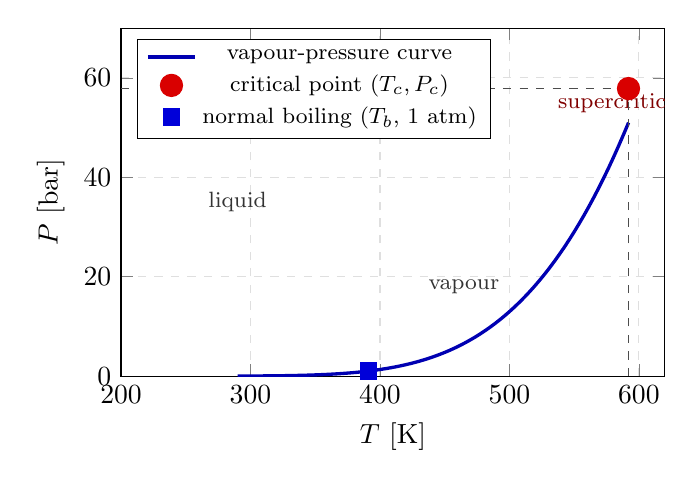
\begin{tikzpicture}
\begin{axis}[
    width=0.7\linewidth, height=6cm,
    xlabel={$T$ [K]},
    ylabel={$P$ [bar]},
    xmin=200, xmax=620,
    ymin=0, ymax=70,
    grid=major,
    grid style={gray!25, dashed},
    legend pos=north west,
    legend style={font=\footnotesize},
    every axis title/.style={below=2pt, at={(0.5,1)}, anchor=south},
]
% Saturation curve for acetic acid (Antoine constants from data file)
% log10 Psat[bar] = 4.68206 - 1642.54 / (T - 39.764)
\addplot [domain=290:592, samples=80, blue!70!black, very thick]
  ({x},{10^(4.68206 - 1642.54/(x-39.764))});
\addlegendentry{vapour-pressure curve}
% Critical point
\addplot[only marks, mark=*, mark size=4pt, mark options={red!85!black}]
  coordinates {(591.95, 57.86)};
\addlegendentry{critical point ($T_c, P_c$)}
% Normal boiling point
\addplot[only marks, mark=square*, mark size=3pt, mark options={blue!85!black}]
  coordinates {(391.05, 1.01325)};
\addlegendentry{normal boiling ($T_b$, 1 atm)};
% Regions labels
\node[anchor=west, font=\footnotesize, text=gray!40!black] at (axis cs:260, 35) {liquid};
\node[anchor=west, font=\footnotesize, text=gray!40!black] at (axis cs:430, 18) {vapour};
\node[anchor=west, font=\footnotesize, text=red!50!black] at (axis cs:530, 55) {supercritical};
% Dashed projections
\draw[dashed, gray!60!black, thin] (axis cs:591.95, 0) -- (axis cs:591.95, 57.86);
\draw[dashed, gray!60!black, thin] (axis cs:200, 57.86) -- (axis cs:591.95, 57.86);
\end{axis}
\end{tikzpicture}
\caption{Vapour-pressure (saturation) curve of acetic acid in the
$P$-$T$ plane, computed from the Antoine constants in
\file{data/standards/components/aceticAcid.dat}.  The square marks
the normal boiling point ($T_b = 391$~K at 1~atm).  The curve
terminates at the critical point ($T_c = 591.95$~K, $P_c =
57.86$~bar): beyond it there is no liquid/vapour distinction.}
\label{fig:criticals-PT}
\end{figure}

Two physical readings of the critical point are worth carrying:

\begin{itemize}[leftmargin=*,nosep]
  \item \textbf{It is where liquid and vapour become indistinguishable.}
        Both phases approach a common density as $T \to T_c$;
        the latent heat $\Delta h^{\mathrm{vap}}$ smoothly decays to
        zero (this is exactly what Watson \eqref{eq:integral-watson}
        encodes).
  \item \textbf{It is the upper limit of the saturation curve.}  Any
        Antoine fit, valid by definition only along the
        saturation line, ceases to make sense beyond $T_c$.
        That is why every \code{vaporPressure} block in the data
        files carries a \code{Trange} that always lies below $T_c$.
\end{itemize}

\subsection{The law of corresponding states}

van der Waals' great insight (1873) was that if you express $T$ and
$P$ in units of their critical values, all simple fluids collapse
onto the same curves.  Define the \emph{reduced} coordinates
\begin{equation}
   T_r \;\equiv\; \frac{T}{T_c}, \qquad
   P_r \;\equiv\; \frac{P}{P_c}, \qquad
   V_r \;\equiv\; \frac{V}{V_c},
\end{equation}
and the two-parameter law of corresponding states asserts: any
property expressed in reduced form is the \emph{same function} of
$(T_r, P_r)$ for every fluid.  Argon and methane and benzene,
plotted as $P_r$ versus $T_r$, give one universal saturation curve
to within a few percent.

The simulator exploits this collapse repeatedly without naming it:
\begin{itemize}[leftmargin=*,nosep]
  \item \textbf{Watson} \eqref{eq:integral-watson} writes
        $\Delta h^{\mathrm{vap}}(T) / \Delta h^{\mathrm{vap}}(T_b)
        = [(1 - T_r)/(1 - T_{br})]^{0.38}$ --- a function of the
        single reduced variable $1 - T_r$.
  \item \textbf{Sato-Riedel} \eqref{eq:sato-riedel} for the
        liquid thermal conductivity is a function of $T_r$ and
        $T_{br}$ only.
  \item \textbf{The planned cubic EOS} (SRK/PR, v1.x) writes the
        attractive parameter $a$ as $a(T) = a_c \cdot \alpha(T_r,
        \omega)$, with $\alpha$ a universal function.
\end{itemize}

\begin{intuition}
Corresponding states is what makes a thermophysical-property data
sheet \emph{short}.  Without it, every fluid would need a custom
correlation for every property.  With it, we measure $T_c$, $P_c$
(and one extra parameter --- next subsection) for every component
and reuse universal forms.  This is the same engineering compression
mentioned in Chapter~\ref{ch:three-pillars}: a few numbers per
component, many predictions.
\end{intuition}

\subsection{The acentric factor $\omega$}

Two-parameter corresponding states works for simple, near-spherical
molecules (argon $\sim$0, methane $\sim$0.01).  Real molecules
deviate: longer chains, polar groups, hydrogen bonds all add
\textbf{shape and stickiness} that two scalars cannot capture.
Pitzer's 1955 fix was a third reduced parameter, the
\emph{acentric factor},
\begin{equation}
   \boxed{\;
   \omega \;\equiv\; -\log_{10}\!\left[ P^{\mathrm{sat}}_r(T_r = 0.7) \right] - 1.
   \;}
   \label{eq:criticals-omega}
\end{equation}
The definition takes the reduced saturation pressure at $T_r = 0.7$
(a representative point on the curve) and measures how far below 0.1
it lies.  Simple fluids sit at $\omega \approx 0$ by construction
(argon, oxygen).  Hydrocarbons grow $\omega$ with chain length
($n$-hexane: 0.30; $n$-decane: 0.49).  Hydrogen-bonded and dimerising
species reach $\omega \approx 0.4$--0.7 (water: 0.34; ethanol: 0.65;
acetic acid: 0.47 --- moderated by vapour-phase dimerisation).

With $\omega$ in hand, the corresponding-states recipe becomes
\textbf{three}-parameter: every dimensionless property is some
universal function $f(T_r, P_r, \omega)$.  This is the empirical
backbone of the SRK and PR cubic EOS that will land in v1.x.

\begin{example}[Computing $\omega$ from Antoine for acetic acid]
At $T_r = 0.7$ we need $T = 0.7 \times 591.95 = 414.36$~K.  From
the Antoine constants in
\file{aceticAcid.dat} ($A=4.68206$, $B=1642.54$, $C=-39.764$):
\[
   \log_{10} P^{\mathrm{sat}}_{\mathrm{[bar]}}(414.36)
   = 4.68206 - \frac{1642.54}{414.36 - 39.764}
   = 4.68206 - 4.3863
   = 0.2957,
\]
so $P^{\mathrm{sat}}(414.36) = 1.977$~bar.  In reduced form,
$P^{\mathrm{sat}}_r = 1.977 / 57.86 = 0.0342$, hence
\[
   \omega = -\log_{10}(0.0342) - 1 = 1.466 - 1 = 0.466,
\]
which agrees with the tabulated $\omega = 0.4665$ in the data file
to three significant figures.  Notice that $\omega$ is not an
independent measurement: it is derivable from $T_c$, $P_c$ and a
single $(T, P^{\mathrm{sat}})$ point at $T_r = 0.7$.
\end{example}

\subsection{The compressibility factor $Z$}

The compressibility factor measures how far a real fluid departs
from the ideal-gas law:
\begin{equation}
   Z \;\equiv\; \frac{P V}{n R T}, \qquad
   Z_{\mathrm{ideal gas}} = 1.
\end{equation}
For low pressures, $Z \approx 1$ for any gas.  As $P \to P_c$,
$Z$ drops below 1 (attraction-dominated, vapour denser than ideal)
or rises above 1 (repulsion-dominated, vapour less dense than
ideal) depending on the molecule.  Corresponding states tells us
that $Z(T_r, P_r, \omega)$ is a \emph{universal} function ---
generalised compressibility charts (Pitzer-Curl, Lee-Kesler) tabulate
it once for all fluids. takes the ideal-gas limit $Z = 1$ throughout: justified for
the vapour-pressure ranges of our 9 stock components at ambient
operating pressures, breaks down above $\sim$10~bar.  When a cubic
EOS lands (post-v1) it will compute $Z(T_r, P_r, \omega)$ via the
roots of the appropriate cubic.  The data files already carry all
the inputs.

\subsection{Where critical properties land in the stack}

\begin{figure}[ht]\centering
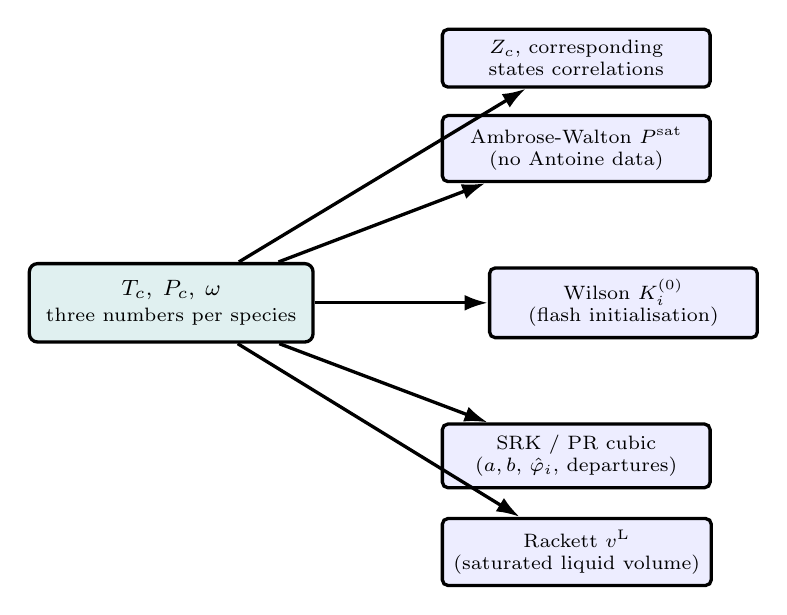
\begin{tikzpicture}[
    >={Latex[width=2.0mm]},
    seed/.style ={draw, rounded corners=3pt, very thick, align=center,
                  inner sep=6pt, minimum width=30mm, font=\footnotesize,
                  fill=teal!12},
    use/.style  ={draw, rounded corners=2pt, very thick, align=center,
                  inner sep=4pt, minimum width=34mm, font=\scriptsize,
                  fill=blue!7},
    flow/.style ={->, very thick},
]
\node[seed] (seed) {$T_c,\;P_c,\;\omega$\\{\scriptsize three numbers per species}};
\node[use, above right=10mm and 16mm of seed] (aw)  {Ambrose-Walton $\Psat$\\(no Antoine data)};
\node[use, right=22mm of seed]                (k0)  {Wilson $K_i^{(0)}$\\(flash initialisation)};
\node[use, below right=10mm and 16mm of seed] (eos) {SRK / PR cubic\\($a,b$, $\hat\varphi_i$, departures)};
\node[use, below right=22mm and 16mm of seed] (rack){Rackett $v^{\mathrm L}$\\(saturated liquid volume)};
\node[use, above right=22mm and 16mm of seed] (zc)  {$Z_c$, corresponding\\states correlations};
\draw[flow] (seed) -- (aw);
\draw[flow] (seed) -- (k0);
\draw[flow] (seed) -- (eos);
\draw[flow] (seed) -- (rack);
\draw[flow] (seed) -- (zc);
\end{tikzpicture}
\caption{The corresponding-states payoff: three numbers per
species --- the critical temperature $T_c$, critical pressure $P_c$, and
acentric factor $\omega$ --- seed an entire thermodynamic stack.  The
same triple supplies the Ambrose-Walton vapour pressure when no Antoine
constants exist, the Wilson $K$-value that initialises every flash, the
$a(T)$ and $b$ of the SRK/PR cubic (and through it $\hat\varphi_i$ and the
enthalpy/entropy departures), the Rackett saturated-liquid volume, and
the generalised $Z_c$ correlations.  Carrying $T_c,P_c,\omega$ in every
component data file is what keeps the stack forward-compatible: select
\code{model SRK;} and those three numbers \emph{become} the equation of
state, no new data required.}
\label{fig:criticals-fanout}
\end{figure}


\begin{center}\small
\begin{tabular}{@{}lll@{}}
\toprule
which property uses it & how & in source code\\
\midrule
$\Delta h^{\mathrm{vap}}(T)$ via Watson         & $T_c$, $T_b$, $\Delta h^{\mathrm{vap}}_{T_b}$  & \code{Component::Hvap\_latent}\\
$\kappa^{\mathrm{liq}}(T)$ via Sato-Riedel    & $T_c$, $T_b$, $M$                              & v1.x roadmap \\
$\varphi_i$ via cubic EOS                       & $T_c$, $P_c$, $\omega$                         & post-v1 \\
$\mu^{\mathrm{gas}}(T)$ via Chapman-Enskog      & $\sigma$, $\epsilon/k$ (correspond to $T_c$, $P_c$)& v1.x roadmap \\
$P^{\mathrm{sat}}(T)$ validity ceiling          & $T_c$ as the upper bound on Antoine \code{Trange} & data-file metadata \\
\bottomrule
\end{tabular}
\end{center}

\begin{intuition}
A practical sanity check when staring at the numbers in a fresh
\file{.dat} file: $T_b/T_c$ should sit in roughly the range
$0.55$--$0.70$ for non-polar molecules (acetic acid: $391/592 =
0.66$; benzene: $353/562 = 0.63$).  If you see $T_b/T_c$ near 1 or
below 0.5, you almost certainly have a data-entry error.  The
ratio $T_b/T_c$ is what Watson, Sato-Riedel and the corresponding-
states machinery rely on; getting it wrong propagates everywhere.
\end{intuition}

% ---------------------------------------------------------------------
\section{Vapour pressure: from Clausius-Clapeyron to Antoine}\label{ch:vap}

\begin{whatyoulllearn}
Antoine is not magic.  It is the engineering refinement of a
thermodynamic identity --- the Clausius-Clapeyron equation --- after
two physical approximations and one empirical fix.  This chapter
walks through that derivation so the three constants $A, B, C$ have
names, the $\log_{10}$ has a reason, and the failure modes of the
correlation are visible by construction.  Watson then enters as the
$\gamma$-$\varphi$-free way to get $\Hvap$ at any $T$ from a single
calorimetric measurement at $T_b$.
\end{whatyoulllearn}

\subsection{The thermodynamic starting point}

Along the liquid-vapour coexistence curve, the chemical potentials
of liquid and vapour are equal: $\mu^{\mathrm{L}}(T,P) =
\mu^{\mathrm{V}}(T,P)$.  Take the differential along the curve,
\[
   \mathrm{d}\mu^{\mathrm{L}} \;=\; \mathrm{d}\mu^{\mathrm{V}}
   \;\Longrightarrow\;
   -s^{\mathrm{L}}\,\mathrm{d}T + v^{\mathrm{L}}\,\mathrm{d}P
   \;=\;
   -s^{\mathrm{V}}\,\mathrm{d}T + v^{\mathrm{V}}\,\mathrm{d}P,
\]
where $s$ and $v$ are the molar entropy and molar volume of each
phase.  Solving for $\mathrm{d}P / \mathrm{d}T$ and using
$\Delta s_{\mathrm{vap}} = \Hvap / T$ (from the Gibbs relation
$\Delta g = 0$ at coexistence) gives the
\textbf{Clausius-Clapeyron equation}:
\begin{equation}
   \boxed{\;
   \frac{\mathrm{d}P^{\mathrm{sat}}}{\mathrm{d}T}
   \;=\; \frac{\Hvap}{T\,\Delta v_{\mathrm{vap}}},
   \;}
   \label{eq:cc-exact}
\end{equation}
where $\Delta v_{\mathrm{vap}} = v^{\mathrm{V}} - v^{\mathrm{L}}$.
Equation~\eqref{eq:cc-exact} is exact: no approximation has been
made.  It is a consequence of the second law (pillar~2 of
Chapter~\ref{ch:three-pillars}) and no fitted constants enter.

\subsection{Two physical approximations}

Equation \eqref{eq:cc-exact} is not yet usable because $v^{\mathrm{V}}$
is itself a function of $T$ and $P$.  Two approximations make it
algebraic:

\begin{enumerate}[leftmargin=*,nosep]
  \item \textbf{The vapour behaves as an ideal gas:}
        $v^{\mathrm{V}} = RT / P^{\mathrm{sat}}$.  Valid well below
        the critical point where vapour density is low.
  \item \textbf{The liquid volume is negligible against the vapour
        volume:} $v^{\mathrm{L}} \ll v^{\mathrm{V}}$.  At 1~bar, $T
        = T_b$, water has $v^{\mathrm{L}} \approx 1.8 \times 10^{-5}$
        m³/mol and $v^{\mathrm{V}} \approx 3.1 \times 10^{-2}$
        m³/mol --- three orders of magnitude apart.  The
        approximation worsens as $T \to T_c$ where the two volumes
        converge.
\end{enumerate}

Under both approximations, $\Delta v_{\mathrm{vap}} \approx RT /
P^{\mathrm{sat}}$, and \eqref{eq:cc-exact} reduces to
\begin{equation}
   \frac{\mathrm{d}P^{\mathrm{sat}}}{\mathrm{d}T}
   \;=\; \frac{\Hvap\,P^{\mathrm{sat}}}{R T^{2}},
\end{equation}
or, dividing through by $P^{\mathrm{sat}}$,
\begin{equation}
   \boxed{\;
   \frac{\mathrm{d}\ln P^{\mathrm{sat}}}{\mathrm{d}T}
   \;=\; \frac{\Hvap}{R T^{2}}.
   \;}
   \label{eq:cc-simple}
\end{equation}
This is the form usually called ``simple Clausius-Clapeyron''.  It
relates the slope of the log-saturation pressure to the latent heat
divided by $RT^{2}$.

\subsection{Integrating with constant $\Hvap$: the rigid form}

The simplest closure is to treat $\Hvap$ as temperature-independent.
Then \eqref{eq:cc-simple} integrates immediately:
\begin{equation}
   \ln P^{\mathrm{sat}}(T) \;=\; -\,\frac{\Hvap}{R\,T} \;+\; C_0,
   \label{eq:cc-rigid}
\end{equation}
where $C_0$ is a constant of integration fixed by one reference point
(e.g.\ the normal boiling point: at $T_b$, $P^{\mathrm{sat}} = 1$~atm).
The rigid form \eqref{eq:cc-rigid} is a straight line on a
$\ln P$-vs-$1/T$ plot, with slope $-\Hvap/R$.

It is also pedagogically powerful: \emph{measuring} $P^{\mathrm{sat}}$
at two temperatures gives you $\Hvap$ from the slope, with no
calorimetry needed.

\begin{intuition}
The rigid form is the simplest closed expression a thermodynamic
identity can be turned into.  Its weakness is the constancy
assumption on $\Hvap$.  Watson \eqref{eq:integral-watson} already
told us $\Hvap$ varies with $T$ --- decaying to zero at $T_c$ ---
so the rigid form must drift from the truth as $T$ moves away from
the reference point.  Across a $100$~K range it is typically wrong
by 5--10\% in $P^{\mathrm{sat}}$, ample reason to want a better fit.
\end{intuition}

\subsection{The empirical fix: Antoine}

What if $\Hvap$ were not constant but \emph{weakly varied} with $T$?
Then \eqref{eq:cc-simple} would integrate to something like
$-\,F(T)/R + C_0$ with $F(T)$ a slowly-varying function.  Fitting a
flexible-enough empirical form to thirty years of measurement
across the laboratory range, Antoine (1888) proposed
\begin{equation}
   \boxed{\;
   \log_{10}\!\Psat_i(T)\,[\text{bar}]
   \;=\; A_i \;-\; \frac{B_i}{T\,[\text{K}] + C_i}.
   \;}
   \label{eq:antoine}
\end{equation}

\begin{figure}[ht]
\centering
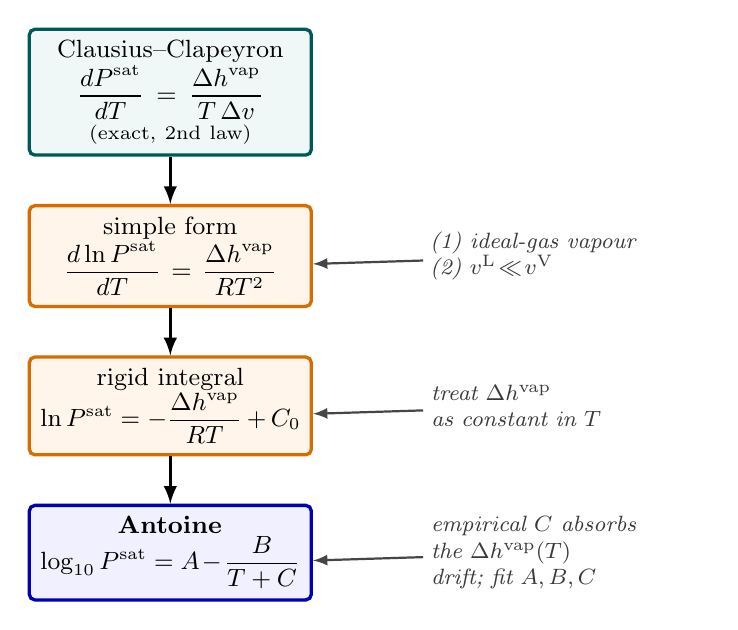
\begin{tikzpicture}[
    node distance=6mm and 9mm,
    box/.style={draw, very thick, rounded corners=2pt, align=center,
                font=\small, inner sep=4pt, minimum height=10mm,
                text width=33mm},
    exact/.style={box, draw=teal!70!black, fill=teal!6},
    approx/.style={box, draw=orange!85!black, fill=orange!8},
    fit/.style={box, draw=blue!70!black, fill=blue!6},
    flow/.style={->, >=latex, very thick},
    note/.style={font=\footnotesize\itshape, text=gray!45!black,
                 align=left, text width=34mm},
]
\node[exact] (cc) {Clausius--Clapeyron\\ $\dfrac{dP^{\mathrm{sat}}}{dT}=\dfrac{\Delta h^{\mathrm{vap}}}{T\,\Delta v}$\\[1pt] \scriptsize(exact, 2nd law)};
\node[approx, below=of cc] (simple) {simple form\\ $\dfrac{d\ln P^{\mathrm{sat}}}{dT}=\dfrac{\Delta h^{\mathrm{vap}}}{RT^2}$};
\node[approx, below=of simple] (rigid) {rigid integral\\ $\ln P^{\mathrm{sat}}=-\dfrac{\Delta h^{\mathrm{vap}}}{RT}+C_0$};
\node[fit, below=of rigid] (ant) {\textbf{Antoine}\\ $\log_{10}P^{\mathrm{sat}}=A-\dfrac{B}{T+C}$};
\draw[flow] (cc) -- (simple);
\draw[flow] (simple) -- (rigid);
\draw[flow] (rigid) -- (ant);
\node[note, right=14mm of simple, anchor=west] (n1)
   {(1) ideal-gas vapour\\ (2) $v^{\mathrm L}\!\ll\! v^{\mathrm V}$};
\node[note, right=14mm of rigid, anchor=west] (n2)
   {treat $\Delta h^{\mathrm{vap}}$\\ as constant in $T$};
\node[note, right=14mm of ant, anchor=west] (n3)
   {empirical $C$ absorbs\\ the $\Delta h^{\mathrm{vap}}(T)$\\ drift; fit $A,B,C$};
\draw[->, >=latex, gray!55!black, thick] (n1) -- ([yshift=-1mm]simple.east);
\draw[->, >=latex, gray!55!black, thick] (n2) -- ([yshift=-1mm]rigid.east);
\draw[->, >=latex, gray!55!black, thick] (n3) -- ([yshift=-1mm]ant.east);
\end{tikzpicture}
\caption{From a thermodynamic identity to the Antoine fit, in three
honest steps.  The exact Clausius--Clapeyron equation (teal, no fitted
constants) becomes algebraic only after \emph{two physical
approximations} (orange): an ideal-gas vapour and a negligible liquid
volume.  Integrating with a constant latent heat gives the rigid
straight-line-on-$\ln P$-vs-$1/T$ form; the empirical Antoine constant
$C$ (blue) then absorbs the temperature drift of $\Delta h^{\mathrm{vap}}$
that the rigid form ignores.  Each downward arrow is a named assumption,
so the student sees exactly what was traded for usability.}
\label{fig:antoine-derivation}
\end{figure}

Recognise the shape: it is the rigid Clausius-Clapeyron form
\eqref{eq:cc-rigid} with one cosmetic and one substantive
modification.

\begin{itemize}[leftmargin=*,nosep]
  \item \textbf{$\log_{10}$ vs $\ln$ (cosmetic).}  Antoine
        historically used base-10 logs because engineers read tables
        with them.  $A \log 10$ and $B \log 10$ differ from the
        natural-log constants by a factor of $\ln 10 \approx 2.303$;
        the physics is unchanged.
  \item \textbf{$T + C$ in the denominator (substantive).}  Instead
        of $1/T$ the denominator is $1/(T + C)$.  The constant
        $C$ absorbs the leading-order temperature dependence of
        $\Hvap$.  In the rigid form $B$ was identified with
        $\Hvap / (R \ln 10)$; in Antoine $B$ no longer has that
        clean meaning, but the three-parameter fit gains an extra
        order of magnitude in accuracy over the same range.
\end{itemize}

\begin{intuition}
The Antoine constants are \emph{not three independent measurements};
they are the three numbers that best track $\ln P^{\mathrm{sat}}$
across the range in which the fit was done.  Reusing them outside
that range is asking the formula to extrapolate.  Asking a fit to
extrapolate is asking the fit to invent.
\end{intuition}

\subsection{Failure modes of Antoine}

Three ways Antoine breaks down, all visible from the structure
of \eqref{eq:antoine}:

\begin{itemize}[leftmargin=*,nosep]
  \item \textbf{Beyond the validity range.}  Antoine is calibrated
        on $[T_{\min}, T_{\max}]$, usually straddling $T_b$.  Push
        far below $T_{\min}$ and the rigid Clausius-Clapeyron
        approximation (constant $\Hvap$) starts to lie; push past
        $T_{\max}$ approaching $T_c$ and \emph{both} approximations
        (constant $\Hvap$ \emph{and} ideal-gas vapour) collapse.
  \item \textbf{$T + C$ flips sign.}  Antoine fits with $C$ negative
        produce undefined logarithms when $T = |C|$.  Typically
        $|C| < T_{\min}$ so this never bites inside the range; if
        you extrapolate below $|C|$ you get a domain error.
  \item \textbf{Near the critical point.}  Above $\sim 0.95\,T_c$
        the vapour is no longer dilute.  No three-parameter form
        can recover the critical exponents; Pitzer/Watson-style
        corresponding-states relations take over.
\end{itemize}

Component data files in \file{data/standards/components/} declare a
\code{Trange} explicitly:
\begin{lstlisting}
vaporPressure
{
    model         Antoine;
    coefficients  (4.68206  1642.540  -39.764);   // aceticAcid
    Trange        (290  392);                     // K
}
\end{lstlisting} does not yet \emph{enforce} the range at run time; this is on
the bug-watch.  But the data are there and the reader of a
\file{.dat} is expected to honour them.

\subsection{Watson for $\Hvap(T)$}

The latent heat is already derived in
Chapter~\ref{ch:integrals}\,(Eq.~\ref{eq:integral-watson}).
Repeated here for completeness:
\begin{equation}
   \Hvap(T) \;=\; \Hvap(T_b)\,
   \biggl(\frac{T_c - T}{T_c - T_b}\biggr)^{0.38}.
\end{equation}
Watson is a corresponding-states result: it depends only on $T_r$
and $T_{br}$, and the $0.38$ exponent is the universal value Watson
extracted from a broad survey of vapour-pressure curves in 1943.
The simulator computes it in \code{Component::Hvap\_latent}.

\subsection{Worked example: water from $\ln P$ vs $1/T$ to Antoine}

\begin{example}[Two ways to compute $\Psat$ of water at 320~K]
Data from
\file{data/standards/components/water.dat} (DIPPR-style, valid
273--373~K): $A = 5.40221$, $B = 1838.675$, $C = -31.737$, $T_b =
373.15$~K, $T_c = 647.10$~K, $\Hvap(T_b) = 40\,650$~J/mol.

\textbf{Antoine, direct.}
\[
   \Psat(320) = 10^{\,5.40221 - 1838.675 / (320 - 31.737)}
   = 10^{\,5.40221 - 6.3781}
   \approx 10^{-0.9759}
   \approx 0.1058~\mathrm{bar}.
\]

\textbf{Rigid Clausius-Clapeyron, for comparison.}  Anchored at
$T_b = 373.15$~K, $\Psat = 1.01325$~bar, using
$\Hvap(T_b) = 40\,650$~J/mol and the rigid form
\eqref{eq:cc-rigid},
\[
   \ln\frac{P^{\mathrm{sat}}(320)}{1.01325}
   = -\frac{40\,650}{8.314}\,\biggl(\frac{1}{320} - \frac{1}{373.15}\biggr)
   \approx -2.171,
\]
giving $\Psat \approx 1.01325 \cdot e^{-2.171} \approx 0.116$~bar.

\textbf{Difference.}  Antoine: $0.106$~bar.  Rigid form: $0.116$~bar.
A $\sim$10\% gap, exactly the order of magnitude we predicted in
\S{Integrating with constant $\Hvap$}.  Antoine wins because its
extra fitted constant $C$ corrects for the weak temperature
dependence of $\Hvap$ that the rigid form ignored.

\textbf{Watson at 320~K, for the energy balance.}
\[
   \Hvap(320) = 40\,650\,
   \left(\frac{647.10 - 320}{647.10 - 373.15}\right)^{0.38}
   \approx 40\,650 \cdot 1.094
   \approx 44\,460~\mathrm{J/mol}.
\]
Water below its boiling point is harder to evaporate than at $T_b$
itself, by about $\sim 9\%$ --- consistent with $\Hvap \to 0$ as $T
\to T_c$ being a slow approach.
\end{example}

\begin{intuition}
Antoine and Watson serve two different masters.  Antoine asks
``what is the saturation pressure?'' --- the answer is needed
\emph{every time} we compute a $K$-value in the flash.  Watson
asks ``how much heat does this phase change move?'' --- the answer
is needed every time the energy balance crosses the L/V boundary
(adiabatic flash, distillation reboiler, condenser duty).  The two
correlations are independent in the simulator; you can use one
without the other.
\end{intuition}

\subsection{Ambrose-Walton: $\Psat$ when there are no Antoine data}\label{sec:ambrose-walton}

\begin{figure}[ht]
\centering
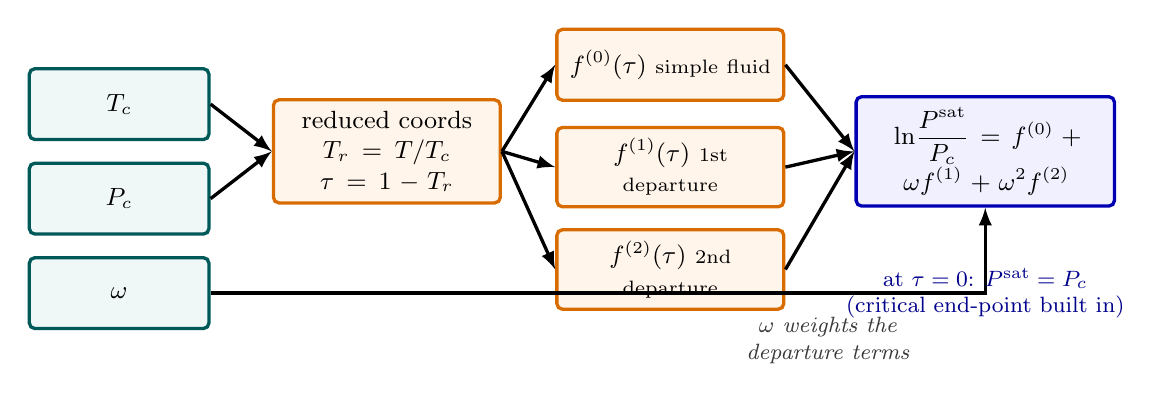
\begin{tikzpicture}[
    box/.style={draw, very thick, rounded corners=2pt, align=center,
                font=\small, inner sep=4pt, minimum height=9mm},
    inp/.style={box, draw=teal!70!black, fill=teal!6, text width=20mm},
    shpx/.style={box, draw=orange!85!black, fill=orange!8, text width=26mm},
    outx/.style={box, draw=blue!70!black, fill=blue!6, text width=30mm},
    flow/.style={->, >=latex, very thick},
]
\node[inp] (tc) at (0,2.0) {$T_c$};
\node[inp] (pc) at (0,0.8) {$P_c$};
\node[inp] (om) at (0,-0.4) {$\omega$};
\node[shpx] (red) at (3.4,1.4) {reduced coords\\ $T_r=T/T_c$\\ $\tau=1-T_r$};
\node[shpx] (f0) at (7.0,2.5) {$f^{(0)}(\tau)$ \scriptsize simple fluid};
\node[shpx] (f1) at (7.0,1.2) {$f^{(1)}(\tau)$ \scriptsize 1st departure};
\node[shpx] (f2) at (7.0,-0.1) {$f^{(2)}(\tau)$ \scriptsize 2nd departure};
\node[outx] (master) at (11.0,1.4)
   {$\ln\!\dfrac{P^{\mathrm{sat}}}{P_c}=f^{(0)}+\omega f^{(1)}+\omega^2 f^{(2)}$};
\draw[flow] (tc.east) -- (red.west);
\draw[flow] (pc.east) -- (red.west);
\draw[flow] (red.east) -- (f0.west);
\draw[flow] (red.east) -- (f1.west);
\draw[flow] (red.east) -- (f2.west);
\draw[flow] (f0.east) -- (master.west);
\draw[flow] (f1.east) -- (master.west);
\draw[flow] (f2.east) -- (master.west);
\draw[flow] (om.east) -| (master.south);
\node[font=\footnotesize\itshape, text=gray!45!black, align=center]
   at (9.0,-1.0) {$\omega$ weights the\\ departure terms};
\node[font=\footnotesize, text=blue!55!black, align=center]
   at (11.0,-0.4) {at $\tau=0$: $P^{\mathrm{sat}}=P_c$\\ (critical end-point built in)};
\end{tikzpicture}
\caption{Ambrose--Walton turns the \emph{three} corresponding-states
constants an estimate already produces ($T_c, P_c, \omega$, teal) into the
\emph{whole} saturation curve, with no measured vapour pressure.  The
reduced temperature feeds three \emph{universal} shape functions
$f^{(0)},f^{(1)},f^{(2)}$ (orange, the same for every fluid); the acentric
factor $\omega$ weights the two departure terms and the sum returns
$\ln(P^{\mathrm{sat}}/P_c)$ (blue).  Because every $f^{(i)}$ vanishes at
$\tau=1-T_r=0$, the curve passes through $P^{\mathrm{sat}}=P_c$ at the
critical point \emph{by construction}---which is exactly what makes a
freshly estimated component flashable.}
\label{fig:ambrose-walton}
\end{figure}


Antoine needs three numbers \emph{fitted to measured vapour
pressures}.  A component you have just \emph{estimated} from its
molecular structure (Joback groups $\to$ $T_c$, $P_c$; Lee-Kesler
$\to \omega$; Chapter~\ref{ch:criticals}) has no such measurements ---
so Antoine cannot be filled, and without $\Psat$ the species is not
flashable.  The Ambrose-Walton correlation closes exactly that gap.
It is a \emph{three-parameter corresponding-states} form: it asks for
only $T_c$, $P_c$ and $\omega$ --- precisely the three constants the
estimate already produced --- and returns the whole saturation curve.

The idea continues the corresponding-states reasoning of
\S\ref{ch:criticals}.  Pitzer's three-parameter principle says the
reduced vapour pressure $\Psat/P_c$ is a \emph{universal} function of
the reduced temperature $T_r = T/T_c$ once the acentric factor
$\omega$ is admitted as a third coordinate.  Expanding $\ln(\Psat/P_c)$
as a power series in $\omega$ and truncating at $\omega^2$,
\begin{equation}\label{eq:aw-master}
   \ln\!\frac{\Psat}{P_c}
   \;=\; f^{(0)}(T_r) \;+\; \omega\,f^{(1)}(T_r)
        \;+\; \omega^2 f^{(2)}(T_r),
\end{equation}
where $f^{(0)}$ is the simple-fluid reference (argon/krypton/xenon,
$\omega \approx 0$) and $f^{(1)}, f^{(2)}$ are the first- and
second-order departures.  Ambrose and Walton (1989) fitted the three
shape functions to high-quality data using a Wagner-style basis in
\[
   \tau \;\equiv\; 1 - T_r,
\]
which vanishes at the critical point and grows toward the triple
point.  Their result, the form the simulator uses verbatim
(\code{AmbroseWalton::psat}), is
\begin{align}
   f^{(0)} &= \bigl(-5.97616\,\tau + 1.29874\,\tau^{1.5}
              - 0.60394\,\tau^{2.5} - 1.06841\,\tau^{5}\bigr)/T_r, \notag\\
   f^{(1)} &= \bigl(-5.03365\,\tau + 1.11505\,\tau^{1.5}
              - 5.41217\,\tau^{2.5} - 7.46628\,\tau^{5}\bigr)/T_r, \label{eq:aw-shape}\\
   f^{(2)} &= \bigl(-0.64771\,\tau + 2.41539\,\tau^{1.5}
              - 4.26979\,\tau^{2.5} + 3.25259\,\tau^{5}\bigr)/T_r. \notag
\end{align}
The fractional powers $\tau^{1.5}$ and $\tau^{2.5}$ are exactly the
Wagner exponents that let a smooth analytic form track the steep
curvature of $\ln\Psat$ down toward the triple point --- the same
curvature Antoine captures with its single empirical constant $C$.
At the critical point $\tau = 0$, every term vanishes, so
$\ln(\Psat/P_c) = 0$, i.e.\ $\Psat = P_c$ at $T = T_c$ \emph{by
construction}.  The simulator caps the output at $P_c$ for any
$T \ge T_c$ (there is no saturation above the critical point).

\paragraph{What the code does.}  \code{AmbroseWalton::psat} is a pure
function of $(T, T_c, P_c, \omega)$ --- it carries no fitted state, so
the estimate op (\code{estimateComponent}) calls the \emph{same}
function to fill a \code{.dat} and the flash calls it at run time.
Note one bookkeeping detail visible in the source: $P_c$ is stored in
\textbf{bar} everywhere in Choupo (as the equations of state also
assume), and the constructor converts it to Pa once so that
\code{Psat\_Pa} returns pure SI.  The three constants are \emph{not}
re-declared inside the \code{vaporPressure} block --- they already
live at component level, and \code{Component::Component} injects them,
so a case author writes only

\begin{lstlisting}
vaporPressure { model AmbroseWalton; }   // Tc, Pc, omega taken from the component
\end{lstlisting}

\begin{example}[Ambrose-Walton $\Psat$ of benzene]
Benzene is a near-simple fluid: $T_c = 562.05$~K, $P_c = 48.95$~bar,
$\omega = 0.210$ (Poling et al., 5th ed., App.~A).  Evaluate at the
normal boiling point $T_b = 353.25$~K --- a self-consistency check,
since the answer should land on $1$~atm.

First the reduced coordinates,
\[
   T_r = \frac{353.25}{562.05} = 0.6285,
   \qquad
   \tau = 1 - T_r = 0.3715 .
\]
The $\tau$ powers: $\tau^{1.5} = 0.22643$, $\tau^{2.5} = 0.08412$,
$\tau^{5} = 0.00708$.  The shape functions from \eqref{eq:aw-shape}
(each already divided by $T_r$):
\[
   f^{(0)} = -3.1574,\quad
   f^{(1)} = -3.3820,\quad
   f^{(2)} = -0.0475 .
\]
Assemble \eqref{eq:aw-master} with $\omega = 0.210$,
\[
   \ln\!\frac{\Psat}{P_c}
   = -3.1574 + (0.210)(-3.3820) + (0.210)^2(-0.0475)
   = -3.8697 ,
\]
so
\[
   \Psat = 48.95\,\mathrm{bar}\times e^{-3.8697}
         = 48.95 \times 0.020862
         = 1.021~\mathrm{bar},
\]
within $0.8\%$ of the $1.013$~bar it \emph{should} return at $T_b$.
The residual gap is honest: $\omega$ here came from a Lee-Kesler
relation, while the saturation curve came from the Ambrose-Walton fit
--- two different correlations, so they disagree by a fraction of a
percent even on a textbook fluid.  At $25\,^\circ$C ($298.15$~K) the
same evaluation gives $0.132$~bar against a measured $\approx
0.127$~bar, about $4\%$ high --- the expected accuracy band for a
constants-only estimate.
\end{example}

\paragraph{Power and limit.}  The power is that Ambrose-Walton needs

\begin{figure}[ht]
\centering
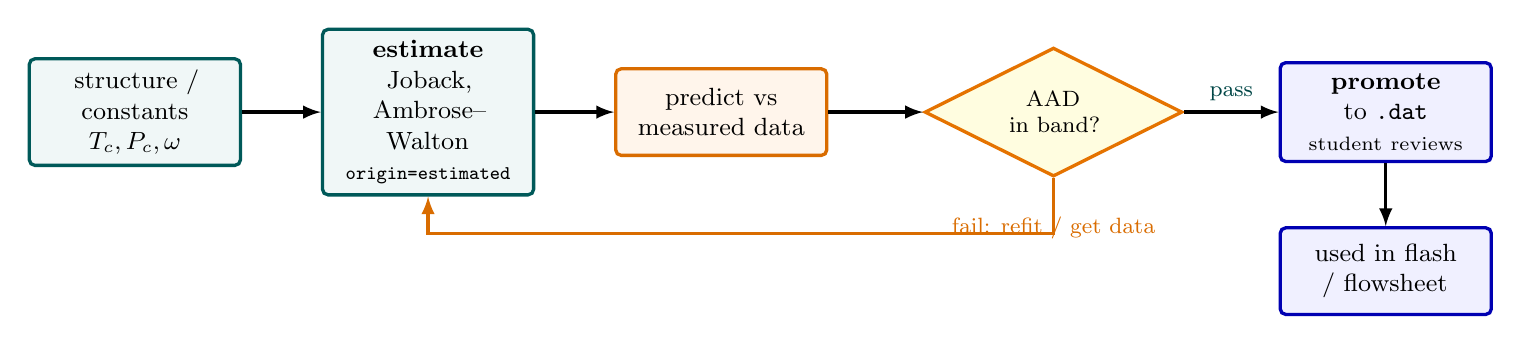
\begin{tikzpicture}[
    node distance=10mm,
    stage/.style={draw, very thick, rounded corners=2pt, align=center,
                  font=\small, inner sep=4pt, minimum height=11mm,
                  text width=24mm},
    create/.style={stage, draw=teal!70!black, fill=teal!6},
    test/.style={stage, draw=orange!85!black, fill=orange!8},
    gate/.style={draw, very thick, fill=yellow!12, draw=orange!90!black,
                 align=center, font=\footnotesize, inner sep=2pt,
                 shape=diamond, aspect=2, text width=18mm},
    use/.style={stage, draw=blue!70!black, fill=blue!6},
    flow/.style={->, >=latex, very thick},
]
\node[create] (struct) {structure / constants $T_c,P_c,\omega$};
\node[create, right=of struct] (est) {\textbf{estimate}\\ Joback, Ambrose--Walton\\ \scriptsize\code{origin=estimated}};
\node[test, right=of est] (pred) {predict vs measured data};
\node[gate, right=12mm of pred] (aad) {AAD\\ in band?};
\node[use, right=12mm of aad] (promote) {\textbf{promote}\\ to \file{.dat}\\ \scriptsize student reviews};
\node[use, below=8mm of promote] (sim) {used in flash / flowsheet};
\draw[flow] (struct) -- (est);
\draw[flow] (est) -- (pred);
\draw[flow] (pred) -- (aad);
\draw[flow] (aad) -- node[above, font=\footnotesize, text=teal!55!black]{pass} (promote);
\draw[flow] (promote) -- (sim);
\draw[flow, orange!85!black] (aad.south) |- ([yshift=-7mm]aad.south)
      node[pos=0.25, below, font=\footnotesize]{fail: refit / get data} -| (est.south);
\end{tikzpicture}
\caption{The glass-box property pipeline: \textbf{estimate}, then
\emph{validate}, then promote.  From a molecular structure or three
critical constants a group-contribution or corresponding-states method
produces a value tagged \code{origin=estimated} (teal).  Before it is
trusted it is compared against measured data and scored by the
average-absolute-deviation (AAD); the gate (yellow) is the project's
no-silent-crutch rule applied to data quality.  Only a value that clears
its accuracy band is \emph{promoted} into the curated \file{.dat} the
student reviews (blue) and the solver then reads.  A failing estimate
loops back to be refitted or replaced by laboratory data---it is never
silently used.}
\label{fig:estimate-validate-promote}
\end{figure}

\emph{nothing measured about the vapour pressure itself}: feed it the
three critical/acentric constants --- which corresponding states gives
you even for a brand-new molecule --- and it returns the entire curve
from triple point to critical point, with the correct critical
end-point built in.  This is what makes an \emph{estimated} component
flashable without a single laboratory point.  The limit is that it is
an \emph{estimate}, not data.  It is good to a few percent for
non-polar and weakly polar species; it \emph{degrades} for strongly
polar, hydrogen-bonding and associating compounds --- water, alcohols,
carboxylic acids --- where the universal $f^{(i)}$ shapes simply do
not describe the real curve.  The glass-box rule therefore stands:
the estimate op overlays the predicted Ambrose-Walton curve on any
measured points in the component's \code{reference\{\}} /
\code{experimental\{\}} blocks, and you look before you trust it for
design.  When you \emph{do} have measured vapour pressures, fit
Antoine (\S\ref{ch:vap}) and use that --- Ambrose-Walton is the
fallback that keeps the simulator running until the data arrive, not a
replacement for them.

\begin{intuition}
Antoine and Ambrose-Walton answer the same question --- ``what is
$\Psat(T)$?'' --- from opposite directions.  Antoine is
\emph{data-first}: three constants regressed from measurements,
accurate inside the fitted window, silent about everything outside it.
Ambrose-Walton is \emph{theory-first}: a universal corresponding-states
shape with no compound-specific tuning beyond $(T_c, P_c, \omega)$,
defined everywhere from triple to critical point but only as accurate
as the universality assumption holds.  A polar molecule breaks the
universality; a molecule outside its Antoine \code{Trange} breaks the
fit.  The honest workflow is to use Antoine where the data live and
fall back to Ambrose-Walton where they do not --- and to plot both
whenever you can.
\end{intuition}

% ---------------------------------------------------------------------
\section{Sublimation: the solid-vapour curve and the triple point}\label{ch:sublimation}

\begin{whatyoulllearn}
The same Clausius-Clapeyron identity that produced Antoine
(\S\ref{ch:vap}) for the liquid-vapour curve produces the
\emph{solid-vapour} (sublimation) curve when the latent heat is the
heat of sublimation rather than of vapourisation.  This section
derives the sublimation line, shows why the three coexistence curves
must meet at one point with $\Hsub = \Hfus + \Hvap$, and documents the
exact algorithm \code{PurePhaseDiagram} uses to draw the
solid/liquid/vapour $P$-$T$ diagram --- sublimation by
Clausius-Clapeyron, melting by the full Clapeyron slope --- so the
triple-point picture of \S\ref{ch:criticals} is finally closed on
both ends.
\end{whatyoulllearn}

\subsection{Why a solid sublimes: the same identity, a different phase}

The derivation of \S\ref{ch:vap} never used the fact that the
condensed phase was a liquid.  It used only that two phases coexist,
so their chemical potentials are equal along the boundary, and that
the Gibbs relation gives $\Delta s = \Delta h / T$ at coexistence.
Replace ``liquid'' by ``solid'' everywhere and the \emph{exact}
Clapeyron equation \eqref{eq:cc-exact} reads, for the solid-vapour
boundary,
\begin{equation}
   \frac{\mathrm{d}P^{\mathrm{sub}}}{\mathrm{d}T}
   \;=\; \frac{\Hsub}{T\,\Delta v_{\mathrm{sub}}},
   \qquad
   \Delta v_{\mathrm{sub}} = v^{\mathrm{V}} - v^{\mathrm{S}},
   \label{eq:clap-sub-exact}
\end{equation}
where $\Hsub$ is the molar enthalpy of sublimation (solid $\to$
vapour, directly, with no liquid in between).  Apply the \emph{same}
two approximations as before --- the vapour is ideal,
$v^{\mathrm{V}}=RT/P$, and the solid volume is negligible against the
vapour, $v^{\mathrm{S}}\ll v^{\mathrm{V}}$ (a solid is even denser
than the liquid, so this is \emph{safer} than for the L/V curve) ---
and \eqref{eq:clap-sub-exact} collapses to the simple form
\begin{equation}
   \frac{\mathrm{d}\ln P^{\mathrm{sub}}}{\mathrm{d}T}
   \;=\; \frac{\Hsub}{R\,T^{2}} .
   \label{eq:cc-sub-simple}
\end{equation}
This is \eqref{eq:cc-simple} with $\Hvap$ swapped for $\Hsub$ ---
``Antoine extended to the solid'', except that we do not bother with a
three-constant Antoine fit here.  Sublimation pressures are tiny and
rarely measured across a wide range, so the simulator integrates
\eqref{eq:cc-sub-simple} in its \emph{rigid} (constant-$\Hsub$) form,
anchored at the triple point $(T_t, P_t)$:
\begin{equation}
   \boxed{\;
   P^{\mathrm{sub}}(T) \;=\;
   P_t \,\exp\!\Bigl[-\frac{\Hsub}{R}
        \Bigl(\frac{1}{T}-\frac{1}{T_t}\Bigr)\Bigr] .
   \;}
   \label{eq:psub}
\end{equation}
This is exactly the line in \code{PurePhaseDiagram::run},
\begin{lstlisting}
const scalar P = Pt * std::exp(-(Hsub / R) * (1.0 / T - 1.0 / Tt));
\end{lstlisting}
evaluated on a grid of $m=\max(6,n/2)$ points from $0.78\,T_t$ up to
$T_t$ (the lower bound keeps $P^{\mathrm{sub}}$ within about three
decades of $P_t$ so it does not vanish off the log axis).

\subsection{The triple point and \texorpdfstring{$\Hsub=\Hfus+\Hvap$}{Hsub=Hfus+Hvap}}

The three coexistence curves --- sublimation (S/V), melting (S/L) and
vapourisation (L/V) --- are not independent.  At the unique
\emph{triple point} $(T_t, P_t)$ all three phases coexist, so the
solid, liquid and vapour chemical potentials are equal there.
Enthalpy is a state function, so the energy to go solid $\to$ vapour
must equal solid $\to$ liquid $\to$ vapour around the triple point:
\begin{equation}
   \boxed{\;\Hsub \;=\; \Hfus \;+\; \Hvap\;}
   \qquad\text{(at the triple point).}
   \label{eq:hsub-sum}
\end{equation}
Because $\Hsub>\Hvap$, the sublimation line is \emph{steeper} than the
vapourisation line on a $\ln P$ vs $1/T$ plot (slope $-\Hsub/R$
against $-\Hvap/R$, both negative): the two curves leave the triple
point at different slopes, with the sublimation curve below and to the
left.  This kink at $T_t$ is the qualitative signature of the triple
point, and \eqref{eq:hsub-sum} is the consistency check the curator
applies before writing a \code{sublimation\{\}} block.

\subsection{The melting line: the full Clapeyron slope}

The solid-liquid boundary is the one curve where neither phase is a
gas, so the ideal-gas trick of \S\ref{ch:vap} is \emph{unavailable}:
$\Delta v_{\mathrm{fus}}=v^{\mathrm{L}}-v^{\mathrm{S}}$ is a small
difference of two condensed-phase volumes, not an $RT/P$ that
dominates.  We must keep the full Clapeyron equation
\eqref{eq:cc-exact}:
\begin{equation}
   \frac{\mathrm{d}P^{\mathrm{fus}}}{\mathrm{d}T}
   \;=\; \frac{\Hfus}{T\,\Delta v_{\mathrm{fus}}} .
   \label{eq:clap-fus}
\end{equation}
Over the modest temperature span of a melting line, $T$ barely moves
from $T_t$ and $\Hfus$, $\Delta v_{\mathrm{fus}}$ are nearly constant,
so \eqref{eq:clap-fus} integrates to a near-straight, very steep line.
The simulator linearises it directly, anchored at the triple point:
\begin{equation}
   T^{\mathrm{fus}}(P) \;=\;
   T_t \;+\; \frac{T_t\,\Delta v_{\mathrm{fus}}}{\Hfus}\,(P - P_t),
   \label{eq:tfus}
\end{equation}
the line \code{const scalar T = Tt + (Tt * dVfus / Hfus) * (P - Pt)}
in \code{PurePhaseDiagram}, swept from $P_t$ up to $\max(P_c,10^8$~Pa$)$.
The sign of $\Delta v_{\mathrm{fus}}$ is what makes water famous: for
almost every substance the solid is denser than the liquid, so
$\Delta v_{\mathrm{fus}}>0$ and the melting line leans \emph{right}
(higher pressure raises the melting point).  Water is the anomaly ---
ice floats, so $\Delta v_{\mathrm{fus}}<0$ and the line leans
\emph{left} (pressure \emph{lowers} the melting point).  In
\file{phase01\_water\_full} the curator enters
\code{deltaVfus -1.63e-6} (m$^3$/mol, \emph{negative}), and the
melting line tilts the right way by construction.

\subsection{What the algorithm needs --- and what it draws}

\code{PurePhaseDiagram} reads the solid anchor from two places, in
precedence order (this matches the code exactly):
\begin{enumerate}[leftmargin=*,nosep]
  \item the component's curated \code{sublimation\{\}} block ---
        \code{tripleT}~$T_t$, \code{tripleP}~$P_t$, \code{Hfus}, \code{Hsub}
        --- the intrinsic pure-compound constants that live \emph{with}
        the species (\code{Component::subTripleT()} etc.);
  \item the op-dict \code{solid\{\}} block, which fills any field the
        component left blank \emph{and} is the sole source of
        \code{deltaVfus}~$\Delta v_{\mathrm{fus}}$ --- the fusion-line
        slope, deliberately kept out of the component block because it
        is a sample/measurement quantity, not a clean intrinsic constant.
\end{enumerate}
The drawing logic then branches on what is available:
\begin{itemize}[leftmargin=*,nosep]
  \item \textbf{L/V only} (no solid anchor): the saturation curve runs
        from $0.45\,T_c$ to $T_c$ and the critical point is marked ---
        the historical behaviour, every existing \code{.dat}
        unaffected.
  \item \textbf{$+$ sublimation} ($T_t,P_t,\Hsub$ all present, flag
        \code{hasSub}): the saturation curve now starts at $T_t$, the
        sublimation curve \eqref{eq:psub} is drawn, and the triple
        point is marked.
  \item \textbf{$+$ fusion} (additionally $\Hfus>0$ and
        $\Delta v_{\mathrm{fus}}\neq0$, flag \code{hasFusion}): the
        melting line \eqref{eq:tfus} is added.
\end{itemize}
Each row of the output CSV is tagged \code{saturation}, \code{sublimation},
\code{fusion}, \code{triple} or \code{critical}, so the GUI can colour the
three curves and place the two singular points without re-deriving anything.

\begin{example}[Triple-point closure for water]
\file{tutorials/props/scan/phase01\_water\_full} draws the full water
diagram with the op-dict anchor
\[
   T_t = 273.16~\mathrm{K},\quad
   P_t = 611.657~\mathrm{Pa},\quad
   \Delta H_{\mathrm{fus}} = 6010,\quad
   \Delta H_{\mathrm{sub}} = 51059~\mathrm{J/mol}.
\]
\textbf{Consistency by \eqref{eq:hsub-sum}.}  The implied heat of
vapourisation at the triple point is
$\Hvap = \Hsub-\Hfus = 51059-6010 = 45049$~J/mol, against the
calorimetric $\approx 45\,054$~J/mol for water at $0\,^\circ$C --- the
block is internally consistent to better than $0.02\%$.

\textbf{A point on the sublimation curve.}  Evaluate
\eqref{eq:psub} at $T = 260$~K (ice subliming below freezing):
\[
   P^{\mathrm{sub}}(260)
   = 611.657\,
     \exp\!\Bigl[-\frac{51059}{8.31446}
        \Bigl(\tfrac{1}{260}-\tfrac{1}{273.16}\Bigr)\Bigr]
   = 611.657\,e^{-1.1383}
   = 195.9~\mathrm{Pa},
\]
about $1.96$~mbar --- the vapour pressure of ice at $-13\,^\circ$C,
within a few percent of the tabulated $\approx 196$~Pa, and the basis
of freeze-drying (lyophilisation): pull the chamber below $P_t$ and
ice leaves as vapour without ever melting.

\textbf{The melting tilt.}  With $\Delta v_{\mathrm{fus}}=-1.63\times
10^{-6}$~m$^3$/mol, the slope \eqref{eq:tfus} is
\[
   \frac{\mathrm{d}T}{\mathrm{d}P}
   = \frac{T_t\,\Delta v_{\mathrm{fus}}}{\Hfus}
   = \frac{273.16\times(-1.63\times10^{-6})}{6010}
   = -7.4\times10^{-8}~\mathrm{K/Pa},
\]
i.e.\ raising the pressure by $100$~bar ($10^7$~Pa) lowers the melting
point by about $0.74$~K --- the classic regelation number, and
negative, as only water and a handful of other anomalies are.
\end{example}

\begin{intuition}
Dry ice and water ice are the two halves of the same picture.
CO\textsubscript{2} has its triple point \emph{above} 1~atm
($T_t=216.6$~K, $P_t=5.18$~bar), so at atmospheric pressure the liquid
field is never crossed: warm a block of solid CO\textsubscript{2} and
it goes straight to gas along the sublimation curve --- that is why it
is ``dry''.  Water's triple point is \emph{below} 1~atm
($611$~Pa), so at room pressure you cross the melting line first and
ice becomes a puddle.  Same three curves, same Clausius-Clapeyron
slope $-\Hsub/R$; the only thing that decides ``dry'' versus ``wet''
is whether the ambient pressure sits above or below $P_t$.
\end{intuition}

\paragraph{Power and limit.}  The power is reuse: one identity
(Clausius-Clapeyron) plus one bookkeeping law ($\Hsub=\Hfus+\Hvap$)
gives the entire solid region from four curated numbers, with the
triple point and critical point as the two anchors that make the
diagram close.  The limit is the same constant-$\Hsub$ rigidity that
makes the rigid L/V form \eqref{eq:cc-rigid} only approximate:
\eqref{eq:psub} treats $\Hsub$ as temperature-independent, exact only
near $T_t$ and drifting as $T$ falls (which is why the curve is drawn
only down to $0.78\,T_t$); and the melting line \eqref{eq:tfus} is
linearised, fine over its narrow span but never extrapolate it to the
exotic high-pressure ice polymorphs.  As always in Choupo, the diagram
is \emph{drawn, not asserted}: the CSV carries every $(T,P)$ point and
its curve tag, so a student sees the kink at the triple point and the
direction of the melting tilt rather than taking them on faith.

% ---------------------------------------------------------------------
\section{Saturated-liquid molar volume: the Rackett equation}\label{ch:rackett}

Ambrose-Walton (\S\ref{sec:ambrose-walton}) gave us $\Psat(T)$ from the
same three constants $(T_c, P_c, \omega)$ an estimate produces.  Its
sibling on the \emph{liquid} side answers the companion question: how
much volume does one mole of saturated liquid occupy?  The simulator
needs this in three independent places --- the liquid \textbf{density}
reported for any stream (\code{ThermoPackage::density}), the
pure-component liquid molar volumes $V_i^L$ that Wilson's
$\Lambda_{ij}=\tfrac{V_j^L}{V_i^L}\exp(\cdots)$ demands
(\eqref{eq:wilson-Lambda}), and the \code{Vliq} field an
\code{estimateComponent} writes into a fresh \code{.dat}.  All three
route through one closure, \code{closures::rackettVliq}, so that what
the estimate stores and what the flash later reads are the \emph{same}
number from the \emph{same} formula --- the glass-box invariant we hold
for every estimated property.

\subsection{Why a special correlation for the liquid?}

A cubic equation of state (SRK, PR; Chapter~\ref{ch:cubic-eos}) will happily
return a liquid root $v^L$, but that root is the EoS's notorious weak
spot: SRK over-predicts saturated-liquid volumes by $10$--$30\%$, and
even the volume-translated forms drift with temperature.  The liquid is
nearly incompressible, so its molar volume is governed almost entirely
by how close $T$ sits to $T_c$ --- a one-dimensional problem along the
saturation line --- and a purpose-built corresponding-states
correlation beats a general EoS by an order of magnitude here.  That
correlation is Rackett's.

\subsection{From the critical point to the Rackett equation}

Start at the critical point, where by definition
\begin{equation}
   Z_c \;=\; \frac{P_c V_c}{\Rgas T_c},
   \qquad\text{so}\qquad
   V_c \;=\; \frac{\Rgas T_c}{P_c}\,Z_c .
\end{equation}
Rackett (1970) observed that if you plot $\ln V^{\mathrm{sat}}$ against
$(1-T_r)^{2/7}$ for a saturated liquid, the data fall on a remarkably
straight line that, extrapolated to $T_r\to 1$, passes through $V_c$.
Anchoring the line at the critical point and letting its slope be set by
$Z_c$ gives the one-constant Rackett equation,
\begin{equation}\label{eq:rackett-raw}
   V^{\mathrm{sat}}(T)
   \;=\; V_c\,Z_c^{\,(1-T_r)^{2/7}}
   \;=\; \frac{\Rgas T_c}{P_c}\,Z_c^{\,1+(1-T_r)^{2/7}},
   \qquad T_r = \frac{T}{T_c} .
\end{equation}
The two forms are identical: substituting $V_c=(\Rgas T_c/P_c)Z_c$ folds
the leading $Z_c$ into the exponent, raising the $1$.  The peculiar
exponent $2/7\approx 0.2857$ is purely empirical --- it is the power
that linearises the most species at once --- and the same $2/7$ you will
see in COSTALD and other liquid-volume correlations descends from
Rackett.  At $T=T_c$ the bracket $(1-T_r)^{2/7}=0$, the exponent is $1$,
and \eqref{eq:rackett-raw} returns exactly $V_c$, as a correlation
seeded at the critical point must.

\subsection{The Spencer-Danner / Yamada-Gunn substitution: \texorpdfstring{$Z_c \to Z_{RA}$}{Zc to ZRA}}

Equation~\eqref{eq:rackett-raw} has a flaw: the \emph{true} $Z_c$ is
itself only known to a percent or two, and using it makes the
correlation miss the actual measured volume at lower $T_r$ where you
care most.  Spencer and Danner (1972) fixed this by replacing $Z_c$ with
an \emph{adjustable} Rackett parameter $Z_{RA}$ --- a number fitted per
compound so that \eqref{eq:rackett-raw} hits one known liquid density.
$Z_{RA}$ is numerically close to $Z_c$ but not equal to it.  When a
fitted $Z_{RA}$ is \emph{not} available --- exactly the situation for an
estimated component --- Yamada and Gunn (1973) supplied a
corresponding-states correlation for it in terms of the acentric factor,
\begin{equation}\label{eq:zra-yamada}
   Z_{RA} \;=\; 0.29056 \;-\; 0.08775\,\omega .
\end{equation}
This is the form the simulator hard-codes.  The constant
$0.29056$ is the generic small-molecule $Z_c\approx 0.29$; the
$-0.08775\,\omega$ term shrinks it as molecules become more elongated
and acentric, mirroring how $Z_c$ falls along a homologous series.
Putting \eqref{eq:zra-yamada} into \eqref{eq:rackett-raw} is the
operational formula:
\begin{equation}\label{eq:rackett-code}
   \boxed{\;
   V^{L}(T)
   \;=\; \frac{\Rgas T_c}{P_c}\;
         Z_{RA}^{\,1+(1-T_r)^{2/7}},
   \qquad
   Z_{RA} = 0.29056 - 0.08775\,\omega .
   \;}
\end{equation}

\paragraph{What the code does.}
\code{closures::rackettVliq(T, Tc, Pc\_Pa, omega)} is
\eqref{eq:rackett-code} verbatim: it forms $T_r=T/T_c$, computes
$Z_{RA}=0.29056-0.08775\,\omega$, raises it to $1+(1-T_r)^{2/7}$, and
multiplies by $\Rgas T_c/P_c$ (note $P_c$ passed in \textbf{Pa} here, so
the result is SI, $\mathrm{m^3/mol}$).  Like the Ambrose-Walton closure
it carries no fitted state --- the estimate op and the run-time density
call the identical function.  This correlation is variously labelled
``Rackett'', ``modified Rackett (Spencer-Danner)'' or
``Rackett/Yamada-Gunn'' depending on whether $Z_{RA}$ is fitted or
predicted; Choupo predicts it from $\omega$, so the diagnostic JSON tags
the value \code{Rackett / Yamada-Gunn}.

\subsection{Mixtures: mole-weighted molar volume}

For a liquid mixture the simulator does \emph{not} mix the constants;
it computes each pure-component saturated volume at the mixture $T$ and
mole-averages them (\code{ThermoPackage::density}, branch~(3)),
\begin{equation}\label{eq:rackett-mix}
   V^{L}_{\mathrm{mix}}(T,\mathbf{x})
   \;=\; \sum_i x_i\,V_i^{L}(T)
   \;=\; \sum_i x_i\,\frac{\Rgas T_c^{(i)}}{P_c^{(i)}}\,
         Z_{RA,i}^{\,1+(1-T/T_c^{(i)})^{2/7}},
\end{equation}
and the reported liquid density is then
$\rho = \overline{M}/V^{L}_{\mathrm{mix}}$ with $\overline{M}=\sum_i
x_i M_i$ the mole-averaged molar mass.  This is the simplest
defensible mixing rule: it assumes an \emph{ideal liquid mixture} (no
excess volume, $V^E=0$), so the partial molar volume of each species
equals its pure-component value.  It is the same Amagat-additivity
assumption that underlies treating the liquid as volumetrically ideal,
and it is exactly the assumption Wilson's $V_j^L/V_i^L$ ratio also
makes.  Real mixtures show a few-percent $V^E$ (ethanol-water famously
contracts), which this rule does not capture --- the honest limit
flagged below.

\begin{example}[Rackett liquid volume and density of benzene]
Benzene: $T_c=562.05$~K, $P_c=48.95$~bar $=4.895\times10^{6}$~Pa,
$\omega=0.210$, $M=78.11$~g/mol.  Evaluate at $25\,^\circ$C
($T=298.15$~K), the temperature \code{estimateComponent} pins.

Reduced temperature and the Rackett parameter,
\[
   T_r = \frac{298.15}{562.05} = 0.5305,
   \qquad
   Z_{RA} = 0.29056 - 0.08775(0.210) = 0.27213 .
\]
The exponent,
\[
   1 + (1-T_r)^{2/7}
   = 1 + (0.4695)^{0.2857}
   = 1 + 0.8084 = 1.8084 .
\]
The prefactor,
\[
   \frac{\Rgas T_c}{P_c}
   = \frac{8.314\times 562.05}{4.895\times10^{6}}
   = 9.547\times10^{-4}~\mathrm{m^3/mol} .
\]
Assemble \eqref{eq:rackett-code},
\[
   V^L = 9.547\times10^{-4}\times (0.27213)^{1.8084}
       = 9.547\times10^{-4}\times 0.09367
       = 8.94\times10^{-5}~\mathrm{m^3/mol}
       = 89.4~\mathrm{cm^3/mol} .
\]
The measured saturated-liquid volume of benzene at $25\,^\circ$C is
$\approx 89.4$~cm$^3$/mol --- agreement to better than $1\%$ for a
non-polar, near-spherical molecule.  The density follows,
\[
   \rho = \frac{M}{V^L}
        = \frac{78.11\times10^{-3}~\mathrm{kg/mol}}
               {8.94\times10^{-5}~\mathrm{m^3/mol}}
        = 874~\mathrm{kg/m^3},
\]
against the handbook $874$~kg/m$^3$.  Rackett is at its best precisely
here.
\end{example}

\paragraph{Power and limit.}  The power mirrors Ambrose-Walton's: from
only $(T_c, P_c, \omega)$ --- the three constants corresponding states
hands you even for a freshly estimated molecule --- Rackett returns the
whole saturated-liquid volume curve, correct to $1$--$2\%$ for normal
fluids and seeded exactly at the critical point.  It is far better than
reading the liquid root of a cubic EoS, and it costs one \code{pow}.
The limits are three.  (i) It is a \emph{saturated}-liquid correlation:
it carries \emph{no} pressure dependence, so it ignores the (small)
compression of a sub-cooled liquid above its saturation pressure --- a
good approximation because liquids are nearly incompressible, but not
exact for high-pressure work.  (ii) Accuracy \emph{degrades} for the
same polar, hydrogen-bonding species that defeat Ambrose-Walton ---
water, alcohols, acids --- because the universal $Z_{RA}(\omega)$ shape
no longer describes them; with a measured density you should fit
$Z_{RA}$ (Spencer-Danner) rather than predict it from $\omega$.
(iii) The mole-weighting \eqref{eq:rackett-mix} assumes $V^E=0$, so it
misses the volume change on mixing of strongly non-ideal solutions.
For pedagogy and for the density figure on a flowsheet stream these are
acceptable; for a custody-transfer liquid density they are not, and the
glass-box rule applies --- the estimate op overlays the Rackett curve on
any measured liquid densities in the component file so you look before
you trust it.

\begin{intuition}
Ambrose-Walton and Rackett are the two halves of one
corresponding-states bargain.  Give up three constants
$(T_c,P_c,\omega)$ and you get back \emph{both} legs of the saturation
envelope --- the pressure $\Psat(T)$ \emph{and} the liquid volume
$V^L(T)$ --- each anchored at the critical point and each accurate to a
few percent for normal fluids.  Neither needs a single measurement of
the property it predicts; both fail on the same polar molecules; both
are fallbacks that keep an estimated component fully simulatable until
real data arrive, and both are overlaid on data, never substituted for
it.
\end{intuition}

% ---------------------------------------------------------------------
\section{Heat capacity}\label{ch:heat}

The molar heat capacity is parametrised as a polynomial in temperature:
\begin{equation}
   C_p^{\mathrm{ig}}(T) \;=\; a_0 + a_1 T + a_2 T^2 + a_3 T^3 + a_4 T^4
   \quad[\mathrm{J/(mol\,K)}].
\end{equation}
Two such polynomials per component: one for the ideal gas
($C_p^{\mathrm{ig}}$, used in vapour-phase energy balances) and one for
the liquid ($C_p^L$, used in liquid-phase energy balances).

For an enthalpy difference between $T_{\mathrm{ref}}$ and $T$:
\begin{equation}
   h(T) - h(T_{\mathrm{ref}}) \;=\; \int_{T_{\mathrm{ref}}}^{T} C_p(T')\, dT'.
\end{equation}
With the polynomial form, this integral is closed-form term by term ---
the simulator does it analytically, not by quadrature.

% =====================================================================
\section{From component data to integral properties}\label{ch:integrals}

\begin{whatyoulllearn}
Each \file{data/standards/components/*.dat} file holds a short list of
numbers: $T_c$, $P_c$, $\omega$, $T_b$, $\Delta h^{\mathrm{vap}}_{T_b}$,
$V^{\mathrm{liq}}$, Antoine constants, $c_p$ polynomials.  This chapter
shows what each one \emph{means}, where the simulator reads it, and
how those tiles are assembled into the integral quantities that drive
every energy balance and every Gibbs-energy minimisation:
pure-component enthalpy and entropy, the latent heat at an arbitrary
$T$ via Watson, mixture enthalpy and mixture Gibbs energy, and
Gibbs-Duhem as the consistency check on activity-coefficient fits.
\end{whatyoulllearn}

\subsection{Anatomy of a component data file}\label{ch:integrals-anatomy}

\begin{figure}[ht]
\centering
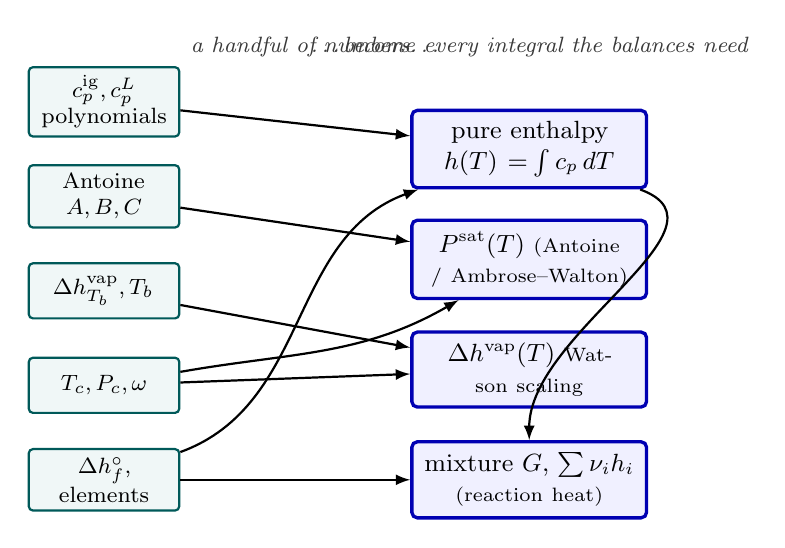
\begin{tikzpicture}[
    tile/.style={draw, thick, rounded corners=1.5pt, align=center,
                 font=\footnotesize, inner sep=3pt, minimum height=7mm,
                 fill=teal!6, draw=teal!70!black, text width=17mm},
    integ/.style={draw, very thick, rounded corners=2pt, align=center,
                  font=\small, inner sep=4pt, minimum height=9mm,
                  fill=blue!6, draw=blue!70!black, text width=27mm},
    flow/.style={->, >=latex, thick},
]
\node[tile] (cp)   at (0,4.2) {$c_p^{\mathrm{ig}},c_p^{L}$ polynomials};
\node[tile] (ant)  at (0,3.0) {Antoine $A,B,C$};
\node[tile] (hvap) at (0,1.8) {$\Delta h^{\mathrm{vap}}_{T_b},T_b$};
\node[tile] (crit) at (0,0.6) {$T_c,P_c,\omega$};
\node[tile] (hf)   at (0,-0.6) {$\Delta h^{\circ}_f$, elements};
\node[integ] (h)   at (5.4,3.6) {pure enthalpy $h(T)=\!\int c_p\,dT$};
\node[integ] (psat) at (5.4,2.2) {$P^{\mathrm{sat}}(T)$ \scriptsize(Antoine / Ambrose--Walton)};
\node[integ] (wat)  at (5.4,0.8) {$\Delta h^{\mathrm{vap}}(T)$ \scriptsize Watson scaling};
\node[integ] (gmix) at (5.4,-0.6) {mixture $G$, $\sum\nu_i h_i$ \scriptsize(reaction heat)};
\draw[flow] (cp) -- (h);
\draw[flow] (hf) to[out=20,in=200] (h);
\draw[flow] (ant) -- (psat);
\draw[flow] (crit) to[out=10,in=210] (psat);
\draw[flow] (hvap) -- (wat);
\draw[flow] (crit) -- (wat);
\draw[flow] (hf) -- (gmix);
\draw[flow] (h) to[out=-20,in=90] (gmix);
\node[font=\footnotesize\itshape, text=gray!45!black] at (2.7,4.9)
   {a handful of numbers\dots};
\node[font=\footnotesize\itshape, text=gray!45!black] at (5.4,4.9)
   {\dots become every integral the balances need};
\end{tikzpicture}
\caption{What a component \file{.dat} file is \emph{for}.  Each entry is a
small tile (teal): a few $c_p$ coefficients, Antoine or critical
constants, a single latent heat at $T_b$, the formation enthalpy and its
element basis.  The simulator assembles those tiles---analytically, term by
term---into the integral quantities (blue) that every energy balance and
every Gibbs-energy minimisation actually consumes: pure-component
enthalpy, the saturation curve, the temperature-corrected latent heat via
Watson, and the mixture Gibbs energy whose $\sum_i\nu_i h_i$ returns the
heat of reaction.  One number can feed several integrals (note the shared
$T_c$ and $\Delta h^{\circ}_f$ arrows).}
\label{fig:dat-to-integrals}
\end{figure}


A typical entry, slightly trimmed for the page:
\begin{lstlisting}
name        aceticAcid;
formula     C2H4O2;
CAS         64-19-7;

MW          60.052;        // kg/kmol
Tc          591.95;        // K
Pc          57.86;         // bar
omega       0.4665;        // [-]
Tb          391.05;        // K
HvapTb      24390;         // J/mol
Vliq        5.752e-5;      // m^3/mol  (57.52 cm^3/mol)

vaporPressure
{
    model         Antoine;
    coefficients  (4.68206  1642.540  -39.764);
    Trange        (290  392);
}

idealGasHeatCapacity {... }
liquidHeatCapacity   {... }
\end{lstlisting}

Each scalar plays a specific role.  The right-hand column below points
to where the simulator reads it:

\begin{center}\small
\begin{tabular}{@{}llp{0.55\linewidth}@{}}
\toprule
field & unit & meaning, and where it is consumed\\
\midrule
\code{MW}        & kg/kmol      &
  Molar mass.  Carries through mass-flow conversions and the sizing
  chapters; entered in every stoichiometry / yield calculation.
  \\
\code{Tc}        & K            &
  Critical temperature.  Sets the upper bound of every saturation
  curve (vapour and liquid become indistinguishable at $T_c$) and is
  the explicit input to the Watson correlation \eqref{eq:integral-watson}.
  Also fed forward to a future SRK/PR EOS.
  \\
\code{Pc}        & bar          &
  Critical pressure.  Carried for the same future EOS work and for
  acentric-factor consistency checks.  Not yet read by the
  ideal-gas $\varphi$.
  \\
\code{omega}     & --           &
  Pitzer's \emph{acentric factor}, defined as
  $\omega = -\log_{10} P^{\mathrm{sat}}_r(T_r = 0.7) - 1$.
  Zero for spherical molecules (argon, methane), positive for
  elongated and hydrogen-bonded ones (acetic acid is on the high
  side at 0.47 because of its dimerisation in the vapour).  Used by
  SRK/PR's $\alpha(T, \omega)$; carries it inertly.
  \\
\code{Tb}        & K            &
  Normal boiling point ($P^{\mathrm{sat}}(T_b) = 1$~atm).  Anchors
  the Watson correlation: the temperature where the latent heat is
  tabulated.  Also a sanity-check ruler for Antoine fits.
  \\
\code{HvapTb}    & J/mol        &
  Latent heat of vaporisation \emph{at $T_b$}, the reference value
  Watson extends to other temperatures.
  \\
\code{Vliq}      & m³/mol       &
  Liquid molar volume at $25\,^\circ$C.  The PFR reads it to convert
  molar feed to a volumetric flow $Q = F \cdot \bar V^{\mathrm{liq}}$
  for the concentration $C_i = F_i / Q$; the stirred-tank sizing
  chain uses it for liquid hold-up.  Treated as constant;
  pressure-volume corrections would be a ten-line edit.
  \\
\code{vaporPressure} & Antoine + Trange &
  $\log_{10} P^{\mathrm{sat}}_{\mathrm{[bar]}} = A - B/(T_{\mathrm{[K]}} + C)$.
  Used everywhere VLE shows up (flash, bubble-T, dew-T, distillation).
  \\
\code{idealGasHeatCapacity} & polynomial &
  $c_p^{\mathrm{ig}}(T) = a_0 + a_1 T + a_2 T^2 + a_3 T^3$,
  J/(mol·K).  Drives the gas-phase part of every energy balance.
  \\
\code{liquidHeatCapacity}    & polynomial &
  Same shape, for the saturated liquid.  Drives the liquid-phase
  part of energy balances and the entropy integral below.
  \\
\bottomrule
\end{tabular}
\end{center}

\begin{intuition}
The data file looks like a flat list of numbers because it
\emph{is} one: a thermodynamic ground truth the simulator's models
do not re-derive, only consult.  Every entry is either
\textbf{measured} (Tc, Pc from Reid/Prausnitz/Poling tables;
Tb, HvapTb from boiling-point calorimetry; Vliq from density at
$25\,^\circ$C; Antoine from regression of vapour-pressure tables;
$c_p$ from calorimetric measurements) or \textbf{empirical}
($\omega$ from a defined regression formula).  Nothing is invented;
nothing is fitted by the simulator at run time.  Chapter~\ref{ch:fittable}
maps out which numbers in the whole stack \emph{would} be fittable in
principle, and which the simulator currently takes as fixed.
\end{intuition}

\subsection{Pure-component enthalpy}

The thermodynamic ground level is fixed by convention: the simulator
sets
\begin{equation}
   h^{\mathrm{liq}}_i(T_{\mathrm{ref}}) \;\equiv\; 0,
   \qquad T_{\mathrm{ref}} \;=\; 298.15~\mathrm{K},
   \label{eq:integral-href}
\end{equation}
for every component in the liquid phase.  Departures from $T_{\mathrm{ref}}$
in the liquid follow from $c_p^{\mathrm{liq}}$:
\begin{equation}
   h^{\mathrm{liq}}_i(T) \;=\; \int_{T_{\mathrm{ref}}}^{T} c_{p,i}^{\mathrm{liq}}(T')\,\mathrm{d}T'.
\end{equation}
With the polynomial $c_p^{\mathrm{liq}} = a_0 + a_1 T + a_2 T^2 + \dots$
shipped in the data file, the integral is term-by-term elementary;
the simulator evaluates it in \file{src/thermo/heatCapacity/Polynomial.cpp},
called via \code{Component::Hliq\_pure(T, Tref)}.

The vapour enthalpy of a pure component sits a latent heat above the
liquid:
\begin{equation}
   \boxed{\;
   h^{\mathrm{vap}}_i(T) \;=\; h^{\mathrm{liq}}_i(T) \;+\; \Delta h^{\mathrm{vap}}_i(T).
   \;}
   \label{eq:integral-hvap}
\end{equation}
The two terms are computed in
\code{Component::Hvap\_pure} / \code{Component::Hliq\_pure} /
\code{Component::Hvap\_latent}; the next subsection is about how the
latent heat at an arbitrary $T$ is obtained from the single tabulated
value $\Delta h^{\mathrm{vap}}_{T_b}$.

\begin{intuition}
The choice $h^{\mathrm{liq}}_i(T_{\mathrm{ref}}) = 0$ is a reference
zero, like sea level in altitude.  For a unit with \emph{no reaction}
only differences enter the energy balance ($h_{\mathrm{out}} -
h_{\mathrm{in}}$, $Q = \dot{n}\,\Delta h_{\mathrm{stage}}$), and the
per-component zero cancels --- a flash, a column, a heater, an
evaporator all balance correctly on this datum.  If you compare these
$h$ values against a table that picked $h^{\mathrm{ig}}_i(298)=0$ for an
\emph{ideal gas} reference, they differ by exactly
$\Delta h^{\mathrm{vap}}_i(T_{\mathrm{ref}})$.

\textbf{But beware: this datum does NOT survive a chemical reaction.}
With a separate zero \emph{for each component}, the difference
$h_B(T) - h_A(T)$ for a reaction $A\!\to\!B$ at fixed $T$ is essentially
zero (both are zeroed at $T_{\mathrm{ref}}$ plus a near-equal sensible
term) --- the heat of reaction has vanished.  An energy balance written
across a reactor on this datum is simply wrong.  The next subsection
fixes this.
\end{intuition}

\subsection{The reference state, and why a reaction needs the elements}
\label{sec:elements-reference}

The sensible+latent datum of the previous subsection sets
$h^{\mathrm{liq}}_i(T_{\mathrm{ref}}) = 0$ \emph{per component} --- every
species gets its own private zero.  That is harmless as long as the set
of species is conserved (no reaction): in $h_{\mathrm{out}} -
h_{\mathrm{in}}$ each species' zero appears once on each side and
cancels.

A reaction breaks that bookkeeping.  Consider the isomerization
$\mathrm{neoC_5} \to n\text{-}\mathrm{C_5}$ (used in the
\file{process05\_isomerization\_recycle} tutorial).  On the per-component
datum, $h_{n\mathrm{C_5}}(T) - h_{\mathrm{neoC_5}}(T) \approx 0$ at equal
$T$, so an energy balance over the reactor reports $\Delta H \approx 0$.
The \emph{true} heat of reaction, however, is the difference of formation
enthalpies,
\begin{equation}
   \Delta h_{\mathrm{rxn}}(T_{\mathrm{ref}}) \;=\;
   \sum_i \nu_i\, \Delta h^{\circ}_{f,i}
   \;=\; \Delta h^{\circ}_{f,n\mathrm{C_5}} - \Delta h^{\circ}_{f,\mathrm{neoC_5}}
   \;=\; -146{,}760 - (-168{,}050)
   \;=\; +21{,}290~\mathrm{J/mol},
\end{equation}
where the index $i$ runs over the \emph{species} taking part in the
reaction and $\nu_i$ is the \textbf{stoichiometric coefficient} of
species $i$ --- \emph{negative for reactants, positive for products}.
For $\mathrm{neoC_5} \to n\text{-}\mathrm{C_5}$ that is
$\nu_{\mathrm{neoC_5}} = -1$ and $\nu_{n\mathrm{C_5}} = +1$, so the sum
is $(+1)\,\Delta h^{\circ}_{f,n\mathrm{C_5}}
  + (-1)\,\Delta h^{\circ}_{f,\mathrm{neoC_5}}$ ---
``products minus reactants'', each weighted by how many moles the
balanced equation consumes or produces.  (The same $i$ indexes a
component everywhere in this guide: $x_i$ its mole fraction, $h_i$ its
molar enthalpy, $\Delta h^{\circ}_{f,i}$ its formation enthalpy.)  The
result is $+21{,}290$~J/mol, i.e.\ \emph{endothermic} --- the isothermal
reactor must be \emph{heated}.  The per-component datum simply cannot
see this number.

The cure is to measure every substance's enthalpy from the same floor:
the \textbf{chemical elements it is made of}, each in its naturally
stable form at $298.15~\mathrm{K},\ 1~\mathrm{bar}$.

\paragraph{What ``the elements datum'' actually means.}
By universal convention, each chemical element is assigned enthalpy
\emph{zero} in its standard state --- its stable form at
$298.15~\mathrm{K}$, $1~\mathrm{bar}$:
\begin{equation*}
   h^{\circ}(\text{C, graphite}) = 0, \quad
   h^{\circ}(\mathrm{H_2}, \text{gas}) = 0, \quad
   h^{\circ}(\mathrm{O_2}, \text{gas}) = 0, \quad
   h^{\circ}(\mathrm{N_2}, \text{gas}) = 0, \;\dots
\end{equation*}
The \textbf{standard enthalpy of formation} $\Delta h^{\circ}_{f,i}$ of
a compound is then the heat of \emph{building one mole of it from those
elements}.  For methane,
\begin{equation*}
   \text{C(graphite)} + 2\,\mathrm{H_2}(\text{gas})
   \;\longrightarrow\; \mathrm{CH_4}(\text{gas}),
   \qquad \Delta h^{\circ}_{f,\mathrm{CH_4}} = -74{,}520~\mathrm{J/mol}.
\end{equation*}
Since the elements on the left are worth zero, the compound's
\emph{absolute} enthalpy on this datum simply \emph{is} its formation
enthalpy: $h^{\circ}_{\mathrm{CH_4}}(298) = \Delta h^{\circ}_{f,\mathrm{CH_4}}
= -74{,}520$~J/mol.  Negative means methane sits \emph{below} its
elements --- energy was released when it formed.

\begin{intuition}
Think of altitude.  Measuring each city's height from its own local
sea level (the per-component datum) is useless for comparing a
Portuguese city with a Spanish one.  Pick \emph{one} global sea level
and all height differences become meaningful.  The chemical elements
are that global sea level for enthalpy: because \emph{every} compound
is measured from the same atomic floor, the atoms cancel in
``products minus reactants'' (mass is conserved in a reaction), and
what is left over is exactly the heat of reaction.  That is why this is
the only datum that survives a reactor.
\end{intuition}

\begin{example}[Burning methane --- the elements never appear in the sum,
yet they make it work]
Everyone knows methane burns and releases a lot of heat.  Let us
\emph{compute} how much, using only formation enthalpies, and watch the
elements datum do its job.  The balanced combustion is
\begin{equation*}
   \mathrm{CH_4} + 2\,\mathrm{O_2} \;\longrightarrow\;
   \mathrm{CO_2} + 2\,\mathrm{H_2O(g)}.
\end{equation*}
Standard formation enthalpies (kJ/mol), straight from the data files:
\begin{center}
\begin{tabular}{lrl}
   \toprule
   species & $\Delta h^{\circ}_{f}$ [kJ/mol] & note \\
   \midrule
   $\mathrm{CH_4}$       & $-74.5$  & a compound \\
   $\mathrm{O_2}$        & $0$      & \textbf{an element --- zero by definition} \\
   $\mathrm{CO_2}$       & $-393.5$ & a compound \\
   $\mathrm{H_2O(g)}$    & $-241.8$ & a compound \\
   \bottomrule
\end{tabular}
\end{center}
Apply ``products minus reactants'', each weighted by its stoichiometric
$\nu$:
\begin{align*}
   \Delta h_{\mathrm{rxn}}
   &= \big[\,1\cdot(-393.5) + 2\cdot(-241.8)\,\big]
      \;-\; \big[\,1\cdot(-74.5) + 2\cdot 0\,\big] \\
   &= (-877.1) - (-74.5) \;=\; \boxed{-802.6~\mathrm{kJ/mol}}.
\end{align*}
Negative and large --- strongly \emph{exothermic}, exactly as the blue
flame on a stove tells you.  Two things to notice.  First, $\mathrm{O_2}$
contributed nothing (it is an element, its enthalpy is the zero of the
scale) --- yet had we measured each compound from its \emph{own} private
zero, the three formation numbers would have been on three incompatible
scales and this subtraction would have been meaningless.  The common
elemental floor is what lets us add them.  Second, no separate ``heat of
reaction'' had to be supplied to the simulator: it is simply
$h_{\mathrm{out}} - h_{\mathrm{in}}$ once every stream carries its
$\Delta h^{\circ}_{f}$.
\end{example}

This is the datum behind $\Delta h^{\circ}_{f,i}$ and the one
\code{Component::h\_pure\_ig} already uses (introduced for the Gibbs
reactor, Chapter~\ref{ch:gibbs-reactor}).  An ideal gas at temperature
$T$ is its formation enthalpy plus the sensible heat from $298.15$~K up
to $T$:
\begin{equation}
   h^{\mathrm{ig}}_i(T) \;=\; \underbrace{\Delta h^{\circ}_{f,i}}_{\text{build it from elements}}
       \;+\; \underbrace{\int_{298.15}^{T} c_{p,i}^{\mathrm{ig}}(T')\,\mathrm{d}T'}_{\text{then heat it to }T}.
\end{equation}
On this datum the liquid sits a latent heat \emph{below} the ideal gas,
so the elements-referenced liquid enthalpy is
\begin{equation}
   \boxed{\;
   h^{\mathrm{liq}}_i(T) \;=\; h^{\mathrm{ig}}_i(T)
       \;-\; \Delta h^{\mathrm{vap}}_i(T),
   \;}
\end{equation}
and now \emph{both} phases share the same zero.  Because each species
carries its $\Delta h^{\circ}_{f,i}$, the sum $\sum_i \nu_i h_i$ over a
reaction returns the heat of reaction automatically --- no separate
$\Delta h_{\mathrm{rxn}}$ term is needed, it falls out of
$h_{\mathrm{out}} - h_{\mathrm{in}}$.  This is the datum every
process simulator uses internally, for exactly this reason.

\begin{intuition}[The standard enthalpy-reference convention]
The standard convention defines the enthalpy reference state as
\emph{the elements at 298.15~K}, with the ideal-gas enthalpy pinned to
the standard heat of formation, $h^{\mathrm{ig}}_i(T_{\mathrm{ref}}) =
\Delta h^{\circ}_{f,i}$ --- the internal calculation path is
elements $\to$ ideal-gas compounds at $298$~K $\to$ ideal gas at $T$
$\to$ real fluid at $T,P$, the same ladder as
Figure~\ref{fig:enthalpy-ladder}.  It is why a stream of pure
ethanol at $298$~K reports a \emph{negative} enthalpy: that number is
its (negative) heat of formation, not a bug.  Choupo follows this
convention, with the reference \emph{pressure} pinned at
$1~\mathrm{bar}$ (the post-1982 NIST/JANAF convention against which the
\code{S\_ig} method was validated).  The gap is \emph{zero} for enthalpy
(ideal-gas $h$ does not depend on pressure) and a flat
$R\ln(1.01325)\approx 0.11~\mathrm{J/(mol\cdot K)}$ for entropy ---
negligible, and never accumulating.
\end{intuition}

\begin{intuition}
Two datums, one rule.  \emph{Sensible+latent} (per-component zero) is
fine for any non-reacting unit and is what the flash / column /
evaporator unit ops use internally for their local duties.  The
\emph{elements} datum (formation-enthalpy zero) is the only one that
survives a reactor, so it is what the \code{energyBalance} report uses
when every component carries a \code{standardThermochemistry} block; the report
falls back to the sensible datum (and flags the row) only when some
species lacks $\Delta h^{\circ}_f$.  The two agree exactly on any unit
where nothing reacts --- which is why \file{flash01} reports the same
$267~\mathrm{kW}$ duty on either datum, while \file{process05}'s
reactor only shows its $+4.5~\mathrm{kW}$ of reaction heat on the
elements datum.
\end{intuition}

The whole picture fits on one ladder.  Figure~\ref{fig:enthalpy-ladder}
stacks the states of a pure substance on a vertical enthalpy axis: the
two candidate zeros, the two latent jumps ($\Delta h^{\mathrm{fus}}$,
$\Delta h^{\mathrm{vap}}$), and the sensible ramps ($\int c_p\,dT$) that
connect them.  Read it once and the reference-state question stops being
mysterious: an enthalpy value is just a \emph{height} on this ladder,
and a "datum" is just the choice of where to nail $h=0$.

\begin{figure}[ht]
\centering
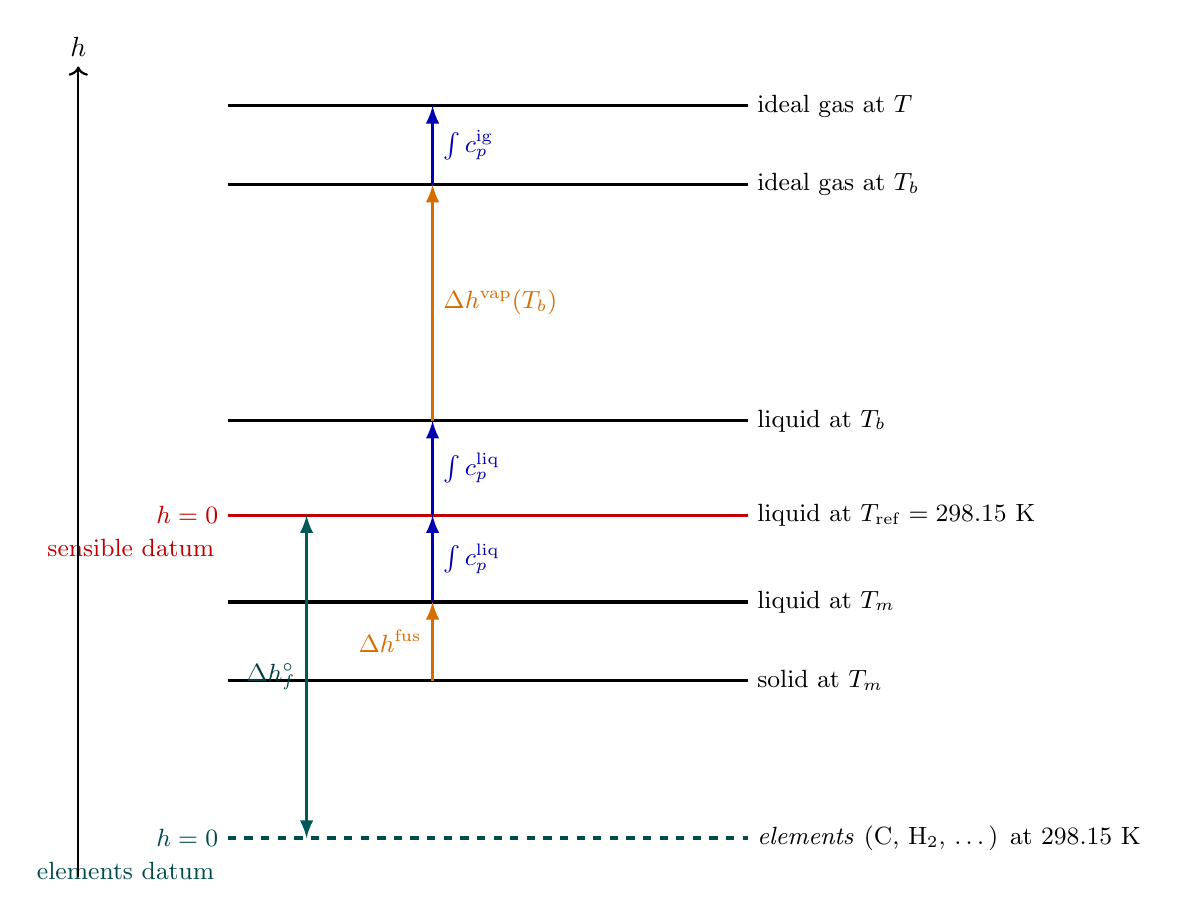
\begin{tikzpicture}[
    state/.style={very thick},
    lat/.style={->, >=latex, orange!85!black, very thick},
    sens/.style={->, >=latex, blue!70!black, very thick},
    form/.style={<->, >=latex, teal!70!black, very thick},
    lbl/.style={font=\small},
    zero/.style={font=\small\bfseries},
]
\def\xl{0}      % left end of state lines
\def\xr{6.6}    % right end of state lines
\def\xa{2.6}    % x of the phase / sensible jump arrows
\def\xf{1.0}    % x of the formation-enthalpy arrow (kept separate)

% --- state levels (y heights, qualitative not to scale) ---
\def\yElem{0}
\def\ySol{2.0}
\def\yLiqM{3.0}
\def\yLiqRef{4.1}
\def\yLiqB{5.3}
\def\yGasB{8.3}
\def\yGasT{9.3}

% horizontal state lines
\draw[state] (\xl,\ySol)   -- (\xr,\ySol);
\draw[state] (\xl,\yLiqM)  -- (\xr,\yLiqM);
\draw[state, red!75!black] (\xl,\yLiqRef) -- (\xr,\yLiqRef);
\draw[state] (\xl,\yLiqB)  -- (\xr,\yLiqB);
\draw[state] (\xl,\yGasB)  -- (\xr,\yGasB);
\draw[state] (\xl,\yGasT)  -- (\xr,\yGasT);
% the elements baseline (dashed, the other candidate zero)
\draw[state, teal!60!black, dashed] (\xl,\yElem) -- (\xr,\yElem);

% state labels (right)
\node[lbl, anchor=west] at (\xr,\ySol)   {solid at $T_m$};
\node[lbl, anchor=west] at (\xr,\yLiqM)  {liquid at $T_m$};
\node[lbl, anchor=west] at (\xr,\yLiqRef){liquid at $T_{\mathrm{ref}}=298.15$~K};
\node[lbl, anchor=west] at (\xr,\yLiqB)  {liquid at $T_b$};
\node[lbl, anchor=west] at (\xr,\yGasB)  {ideal gas at $T_b$};
\node[lbl, anchor=west] at (\xr,\yGasT)  {ideal gas at $T$};
\node[lbl, anchor=west] at (\xr,\yElem)
      {\emph{elements} (C, H$_2$, \dots) at 298.15~K};

% formation enthalpy: its own column on the left, clear of the others
\draw[form] (\xf,\yElem)  -- (\xf,\yLiqRef)
      node[midway, anchor=east, lbl, teal!50!black]{$\Delta h^{\circ}_{f}$};
% phase + sensible jumps
\draw[lat]  (\xa,\ySol)   -- (\xa,\yLiqM)
      node[midway, anchor=east, lbl]{$\Delta h^{\mathrm{fus}}$};
\draw[sens] (\xa,\yLiqM)  -- (\xa,\yLiqRef)
      node[midway, anchor=west, lbl]{$\int c_p^{\mathrm{liq}}$};
\draw[sens] (\xa,\yLiqRef)-- (\xa,\yLiqB)
      node[midway, anchor=west, lbl]{$\int c_p^{\mathrm{liq}}$};
\draw[lat]  (\xa,\yLiqB)  -- (\xa,\yGasB)
      node[midway, anchor=west, lbl]{$\Delta h^{\mathrm{vap}}(T_b)$};
\draw[sens] (\xa,\yGasB)  -- (\xa,\yGasT)
      node[midway, anchor=west, lbl]{$\int c_p^{\mathrm{ig}}$};

% the two candidate zeros, marked
\node[zero, red!75!black, anchor=east] at (\xl,\yLiqRef)
      {\;$h=0$};
\node[lbl, red!75!black, anchor=east] at (\xl-0.05,\yLiqRef-0.42)
      {sensible datum};
\node[zero, teal!60!black, anchor=east] at (\xl,\yElem)
      {\;$h=0$};
\node[lbl, teal!60!black, anchor=east] at (\xl-0.05,\yElem-0.42)
      {elements datum};

% enthalpy axis
\draw[->, thick] (\xl-1.9,-0.5) -- (\xl-1.9,9.8)
      node[anchor=south]{$h$};
\end{tikzpicture}
\caption{The enthalpy ladder of a pure substance (heights qualitative,
not to scale).  Each state is a rung; latent transitions
($\Delta h^{\mathrm{fus}}$, $\Delta h^{\mathrm{vap}}$) and sensible
ramps ($\int c_p\,dT$) connect them.  The \textbf{sensible datum} nails
$h=0$ at the liquid at $T_{\mathrm{ref}}$, \emph{per component} ---
convenient, but every species has its own zero, so it loses the heat of
reaction.  The \textbf{elements datum} nails $h=0$ at the chemical
elements; the rung-to-rung distance up to the substance is its formation
enthalpy $\Delta h^{\circ}_f$, and because all species are measured from
the same elemental floor, $\sum_i \nu_i h_i$ over a reaction returns the
reaction enthalpy automatically.  Choupo's vapour enthalpy is
$h^{\mathrm{vap}} = h^{\mathrm{liq}} + \Delta h^{\mathrm{vap}}$ (one rung
up); on the elements datum the liquid is $h^{\mathrm{ig}} -
\Delta h^{\mathrm{vap}}$ (one rung down from the gas).}
\label{fig:enthalpy-ladder}
\end{figure}

\subsection{Which rung does the data file pin? The \code{phase} keyword}
\label{sec:gibbs-phase}

The ladder of Figure~\ref{fig:enthalpy-ladder} shows that the formation
enthalpy $\Delta h^{\circ}_{f,i}$ is a \emph{distance}: from the elements
baseline (the green dashed line) up to one of the rungs of the species
$i$.  But to which rung exactly?  Different tables answer this question
differently:

\begin{itemize}[leftmargin=*]
  \item NIST and JANAF tabulate $\Delta h^{\circ}_{f,i}$ in the
        \textbf{ideal-gas state at $298.15$~K, $1~\mathrm{bar}$} for
        compounds that can be brought to the gas phase --- water,
        ethanol, methane, the 45 standard volatiles and radicals
        shipped with Choupo.  This is the standard convention
        used internally for every species.
  \item For \textbf{crystalline non-volatiles} that decompose before
        they vaporise (sucrose, glucose, the bulk of solid solutes),
        NIST tabulates $\Delta h^{\circ}_{f}$ in the \textbf{solid}
        state --- there is no honest ideal-gas value to give.
  \item For a small group of compounds (mostly experimentally-measured
        condensed-phase enthalpies of formation), the tabulated number
        is the \textbf{liquid} datum.
\end{itemize}

Choupo records the chosen rung as a one-word field inside the
component's \code{standardThermochemistry} block.  Every entry in
\file{data/standards/components/} declares it explicitly:

\begin{lstlisting}[language=dict]
standardThermochemistry
{
    dHf_298   -241826.0;        // J/mol  (ideal-gas reference)
    s_298     188.834;          // J/(mol*K)  (third-law absolute)
    phase     gas;              // <-- tells the solver which rung
}
\end{lstlisting}

\begin{lstlisting}[language=dict]
standardThermochemistry                  // sucrose, from NIST WebBook
{
    dHf_298   -2226100.0;       // J/mol  (crystalline)
    s_298         392.4;        // J/(mol*K)
    phase     solid;            // <-- never goes through a gas leg
}
\end{lstlisting}

The reason the field matters is operational.  When the energy balance
asks for $h_i^{\mathrm{liq}}(T)$ on the elements datum, the solver
builds a path through the ladder:

\begin{align*}
   \text{natural \code{phase = gas}}: &\quad
       h_i^{\mathrm{liq}}(T) = \Delta h^{\circ}_{f,i}
        + \int_{298.15}^{T} c_p^{\mathrm{ig}}\,dT
        - \Delta h^{\mathrm{vap}}(T) \\
   \text{natural \code{phase = liquid}}: &\quad
       h_i^{\mathrm{liq}}(T) = \Delta h^{\circ}_{f,i}
        + \int_{298.15}^{T} c_p^{\mathrm{liq}}\,dT \\
   \text{natural \code{phase = solid}}: &\quad
       h_i^{\mathrm{liq}}(T) \approx \Delta h^{\circ}_{f,i}
        + \int_{298.15}^{T} c_p^{\mathrm{liq}}\,dT
        \qquad (c_p^{\mathrm{solid}}\!\approx c_p^{\mathrm{liq}},\;
                \Delta h^{\mathrm{fus}}\!\approx 0)
\end{align*}

That is why a sucrose-bearing fermentation stream
\textbf{does not need an ideal-gas $c_p$ for sucrose}: the solver
never integrates through a sucrose vapour leg, because sucrose's
natural rung is on the solid line of the ladder and \code{phase = solid}
tells it so.  Forcing every species through a strict-IG path --- as a
naive strict-IG implementation would --- would require the case
author to invent an artificial $c_p^{\mathrm{ig}}$ for crystalline
sucrose just so the equations work.  Choupo refuses that compromise:
the natural-phase convention keeps the per-species data \emph{honest},
and the energy-balance report still closes through the reactor because
every species carries its own $\Delta h^{\circ}_f$.

\begin{intuition}
Think of \code{phase} as the answer to ``starting from the elements,
where on the ladder does the data sheet stop?''  For gases the table
stops at the top rung (ideal gas at $298$~K).  For sucrose it stops at
the bottom rung (the crystal).  When the energy balance later asks the
liquid enthalpy at some other temperature, the solver knows how to
walk from the recorded rung to the one the balance needs --- and how
to refuse the walk when the latent jump it would need does not exist
(sucrose $\to$ vapour throws a clear error rather than fabricate
numbers).
\end{intuition}

\paragraph{Default for backward compatibility.}
If \code{phase} is absent the solver assumes \code{gas} (the
NIST / JANAF convention, correct for the overwhelming majority of
volatile species).  All standard-catalogue components have been
audited and declare \code{phase} explicitly.  Per-case overlays under
\file{<case>/constant/components/<name>.dat} are subject to the same
rule: new entries should always declare \code{phase} so the datum is
unambiguous at the source of truth.

\subsection{Where every number comes from --- the three questions
            a black-box tool won't answer}
\label{sec:data-provenance-questions}

The \code{phase} keyword of the previous subsection is one instance of a
larger discipline.  The elements datum (\S\ref{sec:elements-reference})
tells you \emph{which floor} a formation enthalpy is measured from; it
does not tell you \emph{where the number on the data sheet came from},
\emph{which model consumed it}, or \emph{at which level of the case it
was overridden}.  A black-box simulator answers none of these: you pick
``Property Method: NRTL-RK'' from a dropdown and a thousand numbers are
sourced, substituted, and defaulted silently behind it.  Choupo's
governing rule is the opposite --- a student points at any number on the
screen and asks \emph{``where did THIS come from?''}, and the run has
already answered it, at the point of use.  Three questions, three rules.

\paragraph{(1) An ``in-water'' property is pair data wearing a
convenience hat.}
The formation enthalpy of crystalline sucrose,
$\Delta h^{\circ}_{f} = -2226.1~\mathrm{kJ/mol}$, is \emph{intrinsic}:
its definition names sucrose and its elements, nothing else.  Its
enthalpy of \emph{solution}, $\Delta h_{\mathrm{soln}} =
+5.40~\mathrm{kJ/mol}$ (crystal $\to$ aqueous), is a different animal:
its definition names \emph{two} species, sucrose \emph{and water}.  That
is \emph{arity-2} data, and it does not live in \file{sucrose.dat} --- it
lives in a by-name catalogue tier,
\file{data/standards/solution/sucrose-water.dat}, exactly as the
infinite-dilution ion enthalpies live in
\file{data/standards/electrolyte/ions.dat} on the
$h^{\circ}_f(\mathrm{H}^+_{aq})=0$ convention.  Water is ubiquitous
enough to earn \emph{one canonical, named aqueous reference tier} ---
never an \emph{implied component slot}.  When a solution property is
needed and no solvent is named, the resolver applies the package default
and \emph{announces it}:
\begin{lstlisting}[language=dict]
[thermo] dHsoln(sucrose): solvent not named -> DEFAULT solvent = water
         source: solution/sucrose-water.dat  [Putnam & Kilday 1986]
\end{lstlisting}
Off-default, it refuses with a remedy rather than silently substitute
the water value.  The student therefore always sees that a second
species was assumed, which one, from which file, and from whose paper
--- the four things a dropdown hides.

\paragraph{(2) A model's parameters live in the model's own block.}
A cubic equation of state (SRK, PR) consumes only the
corresponding-states triad $\{T_c, P_c, \omega\}$ and derives its own
$a_c, b, \kappa$ \emph{in source} --- adding PR after SRK touched no data
file.  A model that needs parameters it \emph{cannot} derive ---
PC-SAFT's segment number $m$, segment diameter $\sigma$, well depth
$\varepsilon/k$ --- carries them in a \emph{model-keyed} sub-block on the
component, \code{eosParameters\{ PCSAFT\{ \ldots \} \}}, each with its own
provenance.  One molecule then carries SRK, PR, PC-SAFT and the next EOS
simultaneously, never colliding, and the run announces \emph{per
component} whether its numbers were derived from corresponding states or
read from a fitted block, and from whose paper:
\begin{lstlisting}[language=dict]
[thermo] EOS = PR     -- benzene: a_c,b,kappa derived from Tc,Pc,omega (intrinsic)
[thermo] EOS = PCSAFT -- benzene: m,sigma,epsilon/k from eosParameters.PCSAFT
                         [Gross & Sadowski 2001]  origin: regressed
\end{lstlisting}
A model missing a required block fails with a remedy --- never a silent
corresponding-states fallback.

\paragraph{(3) A molecule is whole at every level.}
The case tree is fractal (case $\supset$ sector $\supset$ unit), and a
lower node may \emph{overlay} a refined number when its scope makes it
more true --- a particular powder's measured sorption isotherm, say.  But
the overlay is a \emph{patch, never a fork}: the molecule's identity
($\mathrm{MW}, T_c, \omega$) is born once, at the standard tier, and is
the same molecule at every level.  The overlay merges
\emph{block-by-block} --- override the whole \code{solid\{\}}
reference-state block, never a lone scalar inside it (a lone-scalar
overlay would silently splice a sample's $\rho_p$ onto the catalogue's
$k_v$, a hidden hybrid).  And a number that is really a \emph{rate}
(crystallisation kinetics) or a \emph{geometry} (a particle-size
distribution) is not component data at all --- it belongs to the
equipment, in the operation's \code{constant/}, and the PSD travels as a
\emph{stream} attribute.  The cascade line tells the student which level
won.

\begin{intuition}
\emph{All models are wrong, some are useful} --- and Choupo tells you
exactly \emph{which} one you used and \emph{where its numbers came from},
so you judge the usefulness yourself.  A datum's home is decided by
\textbf{arity} (does its definition name a second species?), then by
\textbf{scope} (at what level is it true?), then by \textbf{kind} (is it
the molecule, or the molecule-in-a-machine?).  Nothing --- no solvent, no
model, no level --- is ever implicit on disk.  The curator's full
decision procedure is \file{docs/ai/data-doctrine.md}.
\end{intuition}

\subsection{The Gibbs side: \texorpdfstring{$s^{\circ}_{298}$}{s298}, third-law
entropy, and the absolute ideal-gas free energy}
\label{sec:gibbs-formation-entropy}

The previous subsections settled the \emph{enthalpy} half of the
formation datum: $\Delta h^{\circ}_{f,i}$ pins the substance's height
above the elements floor.  But the Gibbs reactor of
Chapter~\ref{ch:gibbs-reactor} minimises the \emph{Gibbs} energy, and
Eq.~\eqref{eq:gibbs-mu} needs the absolute standard-state free energy
$g^{\circ}_i(T)$, which carries an entropy term.  This subsection
derives the second half of the \code{standardThermochemistry} block --- the
field $s^{\circ}_{298}$ --- and the chain
\code{Component::g\_pure\_ig} walks to assemble $g^{\circ}_i(T)$.

\paragraph{Why entropy needs a \emph{different} reference from enthalpy.}
Enthalpy has no natural zero, so we \emph{chose} one (the elements).
Entropy does have a natural zero: the third law of thermodynamics fixes
$s = 0$ for a perfect crystal at $T = 0$~K.  The number tabulated in
$s^{\circ}_{298}$ is therefore the \textbf{absolute (third-law) entropy}
of the substance at $298.15$~K, $1$~bar --- the integral of $c_p/T$ all
the way up from $0$~K, plus the entropy of every phase change crossed on
the way:
\begin{equation}
   s^{\circ}_{i}(298) \;=\;
   \int_{0}^{298.15} \frac{c_{p,i}(T')}{T'}\,\mathrm{d}T'
   \;+\; \sum_{\text{transitions}} \frac{\Delta h^{\mathrm{trs}}}{T^{\mathrm{trs}}}.
   \label{eq:third-law-entropy}
\end{equation}
This is \emph{not} an ``entropy of formation'' --- it is an absolute
value, and the elements carry a non-zero $s^{\circ}_{298}$ of their own.
That distinction is why the data file stores $\Delta h^{\circ}_{f}$
(a \emph{difference} from the elements) but a plain absolute
$s^{\circ}_{298}$ (a \emph{third-law} value).  The reaction's entropy
change reconstructs automatically as $\sum_i \nu_i\, s^{\circ}_i$,
because the atoms cancel exactly as they did for enthalpy.

\paragraph{From the two stored numbers to $g^{\circ}_i(T)$.}
Both stored values are pinned at $298.15$~K; the simulator transports
them to the reactor temperature $T$ by integrating the ideal-gas heat
capacity.  Enthalpy uses $\int c_p\,dT$, entropy uses
$\int c_p/T\,dT$:
\begin{align}
   h^{\circ}_i(T) &= \Delta h^{\circ}_{f,i}
        \;+\; \int_{298.15}^{T} c_{p,i}^{\mathrm{ig}}(T')\,\mathrm{d}T',
        \label{eq:gibbs-h-of-T}\\[2pt]
   s^{\circ}_i(T) &= s^{\circ}_{i}(298)
        \;+\; \int_{298.15}^{T} \frac{c_{p,i}^{\mathrm{ig}}(T')}{T'}\,\mathrm{d}T',
        \label{eq:gibbs-s-of-T}\\[2pt]
   \boxed{\;g^{\circ}_i(T) \;=\; h^{\circ}_i(T) \;-\; T\,s^{\circ}_i(T).\;}
        \label{eq:gibbs-g-of-T}
\end{align}
These are exactly \code{Component::h\_pure\_ig(T)},
\code{Component::s\_pure\_ig(T)} and
\code{Component::g\_pure\_ig(T)} in
\file{src/thermo/Component.cpp}.  The two integrals are the $H$ and $S$
methods of the heat-capacity model
(\file{src/thermo/heatCapacity/}); for the polynomial form
$c_p^{\mathrm{ig}} = a_0 + a_1 T + a_2 T^2 + a_3 T^3$ both are
elementary:
\begin{equation*}
   \int_{298.15}^{T}\!\! c_p\,dT' = \sum_k \frac{a_k}{k+1}\bigl(T^{k+1} - 298.15^{k+1}\bigr),
   \quad
   \int_{298.15}^{T}\!\! \frac{c_p}{T'}\,dT' =
     a_0 \ln\frac{T}{298.15} + \sum_{k\ge 1} \frac{a_k}{k}\bigl(T^{k} - 298.15^{k}\bigr).
\end{equation*}
The \emph{element-potential} solver of the Gibbs reactor reads only the
combination $g^{\circ}_i(T)/RT$ (it appears as \code{g\_pure\_ig(T)/RT}
in \file{gibbsMethod/ElementPotential.cpp}), so the $1$~bar standard
reference cancels into the $\ln(y_iP)$ term of
Eq.~\eqref{eq:gibbs-mu} and never appears as a separate offset.

\begin{example}[Reforming: the entropy term decides the equilibrium]
The water-gas-shift reaction $\mathrm{CO} + \mathrm{H_2O}
\rightleftharpoons \mathrm{CO_2} + \mathrm{H_2}$ has almost no entropy
change (two moles to two moles), so it is dominated by $\Delta h$; but
the steam-reforming reaction $\mathrm{CH_4} + \mathrm{H_2O}
\rightleftharpoons \mathrm{CO} + 3\,\mathrm{H_2}$ goes from two moles of
gas to four, and $\Delta s^{\circ}$ is large and positive.  Below
$\sim 900$~K the $-T\Delta s$ term in $\Delta g^{\circ} =
\Delta h^{\circ} - T\Delta s^{\circ}$ is too small to overcome the
endothermic $\Delta h^{\circ} \approx +206$~kJ/mol, and equilibrium sits
on the methane side; raise $T$ and the entropy term flips the sign of
$\Delta g^{\circ}$, driving conversion to syngas.  A Gibbs reactor
\emph{cannot} reproduce this temperature swing from
$\Delta h^{\circ}_f$ alone --- it needs each species'
$s^{\circ}_{298}$.  That is why the \code{standardThermochemistry} block carries
\emph{both} numbers, and why a component lacking $s^{\circ}_{298}$
cannot be placed in a Gibbs reactor.
\end{example}

\subsection{Where the two numbers come from: the NASA-CEA import}
\label{sec:gibbs-nasa-import}

A component's $\Delta h^{\circ}_{f}$ and $s^{\circ}_{298}$ are
\emph{curated}, not computed at run time --- they are measured
thermochemistry the simulator only consults.  Choupo's gas-phase
formation data are imported from the \textbf{NASA Glenn} thermodynamic
database (NASA-7 polynomials), via the curation tool
\file{bin/curate/import\_gibbs\_nasa.py}.  The primary source is McBride,
Gordon \& Reno, NASA TM-4513 (1993)\,\footnote{B.~J.~McBride,
S.~Gordon, M.~A.~Reno, \emph{Coefficients for Calculating Thermodynamic
and Transport Properties of Individual Species}, NASA Technical
Memorandum 4513 (1993).  A US-government work, in the public domain;
also the data behind the NASA CEA program (Gordon \& McBride, NASA
RP-1311, 1994).}, a public-domain US-government work.

The connection between a NASA-7 polynomial and the two fields Choupo
needs is direct and exact.  The NASA polynomials are themselves
referenced to the elements, so the standard-state enthalpy they return
at $298.15$~K \emph{is} the enthalpy of formation, and the entropy they
return is the third-law absolute entropy:
\begin{equation}
   \Delta h^{\circ}_{f,i} \;=\; H^{0}_i(298.15),
   \qquad
   s^{\circ}_{i}(298) \;=\; S^{0}_i(298.15),
\end{equation}
which is precisely what the import reads off the polynomial
(\code{standard\_enthalpies\_RT} and \code{standard\_entropies\_R}
evaluated at $298.15$~K, $1$~atm).

\paragraph{Two glass-box guards (why the import is trustworthy).}
The tool refuses to write a number it cannot defend:
\begin{itemize}[leftmargin=*]
  \item \textbf{Anchor verify.}  Before any file is touched, the tool
        re-derives $\Delta h^{\circ}_f$ for five well-known species
        ($\mathrm{CO_2}, \mathrm{H_2O}, \mathrm{NH_3}$, benzene,
        $\mathrm{CO}$) and aborts if any deviates from the textbook
        value by more than $0.5$~kJ/mol --- a unit-conversion or
        transcription slip is caught at the door.
  \item \textbf{Isomer guard.}  NASA names many species by formula only,
        and the trap is real: ``C3H6O'' in TM-4513 is \emph{propylene
        oxide} ($\Delta h^{\circ}_f \approx -93.7$~kJ/mol), not acetone
        ($-217.1$).  Every name-to-NASA mapping therefore carries an
        \emph{expected} $\Delta h^{\circ}_f$, and the import \textbf{refuses}
        any species whose NASA value deviates by more than $5$~kJ/mol.
        A wrong-isomer match is a transcription error to catch, never a
        number to trust.
\end{itemize}
A real, curated measured value already in
\file{data/standards/components/} is never overwritten; the import only
\emph{fills} an absent block or \emph{refits} one tagged as an estimate
(Joback, \code{origin=estimated}).  Species with no clean,
isomer-unambiguous NASA match (acetone, the longer $n$-alkanes, the
xylenes, diethyl ether) are deliberately left carrying their
honestly-tagged Joback estimate rather than a guessed value --- the gap
is kept visible, not papered over.

\begin{intuition}[Power and limit]
\textbf{Power:} two small numbers per species --- $\Delta h^{\circ}_f$
and $s^{\circ}_{298}$ --- plus a $c_p^{\mathrm{ig}}(T)$ polynomial are
enough to give the absolute Gibbs energy of \emph{any} ideal-gas mixture
at \emph{any} temperature, which is all the element-potential equilibrium
solver needs.  The data are public-domain, element-referenced, and
audited.  \textbf{Limit:} the chain is strictly \emph{ideal-gas}.
$g^{\circ}_i(T)$ carries no pressure correction beyond the ideal
$RT\ln(y_iP)$, no real-gas fugacity, and no liquid- or solid-phase
free energy --- so a Choupo Gibbs reactor is a gas-phase equilibrium
tool.  And the values are only as good as the NASA fit: TM-4513
$c_p$ polynomials are reliable to $\sim 1000$--$6000$~K depending on
species, and an estimated (Joback) entry can be off by several kJ/mol,
which the per-value provenance tag makes the student check before
trusting an equilibrium prediction.
\end{intuition}

\subsection{Latent heat at any $T$: Watson}

Each data file lists $\Delta h^{\mathrm{vap}}_i(T_b)$ at the normal
boiling point only.  The simulator transports it to any other
temperature with Watson's correlation,
\begin{equation}
   \boxed{\;
   \Delta h^{\mathrm{vap}}_i(T) \;=\; \Delta h^{\mathrm{vap}}_i(T_b)
     \left(\frac{T_c - T}{T_c - T_b}\right)^{0.38}.
   \;}
   \label{eq:integral-watson}
\end{equation}
This is not a fit; it is a dimensionally motivated power law that
collapses to $\Delta h^{\mathrm{vap}} \to 0$ as $T \to T_c$ (vapour
and liquid become indistinguishable) and reproduces the tabulated
$\Delta h^{\mathrm{vap}}(T_b)$ at $T = T_b$ by construction.  The
exponent $0.38$ is the empirical Watson value; Pitzer's later
acentric-factor formulation refines it but the simple form is good to
a few percent across the practically interesting range $T_b < T <
0.95\,T_c$.

Implementation: \code{Component::Hvap\_latent(T)} in
\file{src/thermo/Component.cpp}, ~6 lines.

\begin{example}[Acetic acid latent heat at $T = 350$~K]
With $T_c = 591.95$~K, $T_b = 391.05$~K, $\Delta h^{\mathrm{vap}}_{T_b}
= 24{,}390$~J/mol from \file{data/standards/components/aceticAcid.dat},
\[
   \Delta h^{\mathrm{vap}}(350)
   \;=\; 24390 \cdot
   \left(\frac{591.95 - 350}{591.95 - 391.05}\right)^{0.38}
   \;\approx\; 24390 \cdot (1.2042)^{0.38}
   \;\approx\; 26{,}120~\mathrm{J/mol}.
\]
Acetic acid is harder to evaporate at 350~K than at its boiling point
(by $\sim 7\%$).  The trend is universal: $\Delta h^{\mathrm{vap}}$
\emph{decreases} as $T$ rises toward $T_c$.
\end{example}

\subsection{Pure-component entropy and Gibbs energy}

Entropy is the analogous integral against $c_p / T$,
\begin{equation}
   s^{\mathrm{liq}}_i(T) - s^{\mathrm{liq}}_i(T_{\mathrm{ref}})
   \;=\; \int_{T_{\mathrm{ref}}}^{T} \frac{c_{p,i}^{\mathrm{liq}}(T')}{T'}\,\mathrm{d}T',
\end{equation}
and the vapour entropy is a latent step above:
\begin{equation}
   s^{\mathrm{vap}}_i(T) \;=\; s^{\mathrm{liq}}_i(T) \;+\;
   \frac{\Delta h^{\mathrm{vap}}_i(T)}{T}.
\end{equation}
With $h$ and $s$ in hand, the pure-component Gibbs energy follows by
the Legendre transform that defines it,
\begin{equation}
   g_i(T) \;=\; h_i(T) - T\,s_i(T),
\end{equation}
and the same reference convention ($g^{\mathrm{liq}}_i(T_{\mathrm{ref}})
= -T_{\mathrm{ref}}\,s_i(T_{\mathrm{ref}})$) is carried through.

\begin{intuition}
None of the unit ops  actually call $s$ or $g$ directly ---
the energy balances are all in $h$ alone, because the systems
considered are non-reactive plus elementary kinetics where $\Delta G$
of reaction is not yet needed.  When chemical-equilibrium reactors
land (post-v1), the same Cp / Watson chain feeds $\Delta G_r =
\Delta h_r - T\,\Delta s_r$ for the equilibrium constant
$K_{\mathrm{eq}}(T) = \exp(-\Delta G_r / RT)$.  Wiring is one
afternoon's work; the data are already in place.
\end{intuition}

\subsection{Mixing: ideal versus real}

The simulator's mixture enthalpy is the ideal-mixing combination of
the pure values, weighted by phase fractions:
\begin{equation}
   h_{\mathrm{mix}}(T) \;=\; (1 - V)\,\sum_i x_i\,h^{\mathrm{liq}}_i(T)
                       \;+\; V\,\sum_i y_i\,h^{\mathrm{vap}}_i(T),
   \label{eq:integral-hmix}
\end{equation}
exactly as implemented in \code{ThermoPackage::Hmixture}.  This
assumes the \emph{excess enthalpy} $h^E$ of mixing is negligible.
For Raoult systems (benzene/toluene, $n$-hexane/$n$-heptane) and
moderately non-ideal systems with weak hydrogen bonding, $h^E$ is
indeed tens of J/mol against pure $h$'s of tens of kJ/mol --- a
sub-percent correction.  For strongly hydrogen-bonded mixtures
(ethanol/water, acetic acid/water) $h^E$ can reach $\sim 500$~J/mol
and the energy balance will under-predict, e.g., the duty of a
condenser by a fraction of a percent up to a few percent.

The Gibbs energy of mixing is where activity coefficients enter.
For a single-phase mixture
\begin{equation}
   \boxed{\;
   \Delta G_{\mathrm{mix}} \;=\; RT\,\sum_i x_i \ln\!\bigl(x_i \gamma_i\bigr)
     \;=\;\underbrace{RT\sum_i x_i \ln x_i}_{\text{ideal mixing, always}\,\le 0}
     \;+\; \underbrace{RT\sum_i x_i \ln \gamma_i}_{\equiv\,G^E,\ \text{excess Gibbs}}.
   \;}
   \label{eq:integral-Gmix}
\end{equation}
The ideal part is the universal $-T\,\Delta s_{\mathrm{mix}}^{\mathrm{ideal}}
= RT \sum x_i \ln x_i$ that always drives mixing forward at finite
$T$ for components that mix at all.  The excess part $G^E$ is what
NRTL, Wilson and friends actually parameterise, via $\ln \gamma_i =
\partial(n\,G^E/RT)/\partial n_i$ at constant $T, P, n_{j\neq i}$.
A consistency check is built in: an activity model has to satisfy
the integrability constraint that follows next.

\subsection{Gibbs-Duhem: the consistency check}

At constant $T$ and $P$, partial molar quantities of a mixture are
not independent.  The Gibbs-Duhem identity for the activity
coefficients reads
\begin{equation}
   \boxed{\;
   \sum_i x_i\,\mathrm{d}(\ln \gamma_i) \;=\; 0
   \quad\text{(constant $T, P$).}
   \;}
   \label{eq:integral-gd}
\end{equation}
It says: you cannot fit $\ln \gamma_1$ and $\ln \gamma_2$ to data
independently and freely --- once $\ln \gamma_1(x_1)$ is chosen,
$\ln \gamma_2(x_1)$ is determined up to a constant of integration
fixed by the pure-limit $\gamma_i(x_i \to 1) = 1$.

For a binary system the constraint linearises to a useful test on
experimental data: at a series of $(x_1, \gamma_1, \gamma_2)$
measurements, the area under $\ln(\gamma_1/\gamma_2)$ over the full
composition range must integrate to zero:
\begin{equation}
   \int_0^1 \ln\frac{\gamma_1(x_1)}{\gamma_2(x_1)}\,\mathrm{d}x_1
   \;=\; 0.
   \label{eq:integral-gd-area}
\end{equation}
This is the celebrated Redlich-Kister consistency test.  When the
\code{fitParameters} regression fits NRTL or Wilson parameters to a
$(x_1, T_{\mathrm{bubble}})$ dataset (the
\file{tutorials/fitNRTL01\_ethanol\_water} case), the chosen
functional form for $G^E$ \emph{automatically} satisfies
Eq.~\eqref{eq:integral-gd} by construction --- NRTL and Wilson are
both derived from a $G^E$ model, and any pair of $\ln \gamma_i$
derived from a single $G^E$ obeys Gibbs-Duhem identically.  The fit
quality therefore measures how well the data themselves are
thermodynamically consistent: a poor LM convergence is sometimes the
data's fault, not the optimiser's.

\begin{pitfall}
Gibbs-Duhem is exact for a binary mixture as written, but its
appearance changes in $n$-component systems --- there it becomes
$\sum_i x_i\,\mathrm{d} \ln \gamma_i = 0$ along any
infinitesimal path in composition space.  Most published binary
$\gamma$-data sets satisfy GD to within experimental noise;
ternary data sets often do not (a hint that one of the three
binaries is missing the cross-term).  If you ever fit a ternary by
combining three independent binary NRTL pairs, you have implicitly
trusted the GD consistency of each pair.
\end{pitfall}

\subsection{Putting it together: an example energy balance}

Take an isobaric heater that brings 100~kmol/h of equimolar
ethanol/water from $T_{\mathrm{in}} = 300$~K to $T_{\mathrm{out}} =
360$~K, no phase change ($V = 0$ throughout, liquid only).  The
duty per kmol of feed is
\begin{align}
   q &\;=\; h_{\mathrm{liq}}(360) - h_{\mathrm{liq}}(300) \notag\\
     &\;=\; \sum_i x_i \bigl[h^{\mathrm{liq}}_i(360) - h^{\mathrm{liq}}_i(300)\bigr] \notag\\
     &\;=\; \sum_i x_i\,\int_{300}^{360} c_{p,i}^{\mathrm{liq}}(T)\,\mathrm{d}T.
\end{align}
Using the constant-$c_p$ approximations shipped 
(ethanol: $c_p^{\mathrm{liq}} \approx 165$~J/(mol·K); water:
$\approx 75.4$~J/(mol·K)), this evaluates to
\[
   q \;\approx\; 0.5 \cdot 165 \cdot 60 + 0.5 \cdot 75.4 \cdot 60
     \;\approx\; 7{,}212~\mathrm{J/mol \ feed}.
\]
At 100~kmol/h that is a duty of about
$7{,}212 \cdot 10^5 / 3600 \approx 200~\mathrm{kW}$ --- which is
exactly what \code{tutorials/hx01\_heater} reports when you run it.
Every step uses only Eqs.~\eqref{eq:integral-href}--\eqref{eq:integral-hmix}
and the polynomial $c_p$ from the data file.

\begin{tutoriallink}
\code{runCase tutorials/hx01\_heater} executes the duty calculation
above end-to-end and writes the result to the run log.  Modify
\file{tutorials/hx01\_heater/system/flowsheetDict} to change
$T_{\mathrm{out}}$ and watch how $Q$ scales linearly with
$\Delta T$ --- a direct consequence of constant $c_p$.
\end{tutoriallink}

\section{What is fittable, what is not}\label{ch:fittable}

Every model in this Part has parameters that ultimately come from
\emph{somewhere}. The simulator distinguishes three sources, in
descending order of trust:

\begin{enumerate}[leftmargin=*,nosep,topsep=2pt]
  \item \textbf{Literature curation.} Antoine constants $(A_i, B_i,
        C_i)$, critical properties $(T_c, P_c, \omega)$, normal
        boiling points, latent heats, heat-capacity polynomials,
        liquid molar volumes --- these live in
        \file{data/standards/components/<name>.dat} and are
        cited per-file at the top of each file. They are
        \emph{not} estimated by the simulator. To add a new component,
        copy an existing \code{.dat} file and populate it from DIPPR /
        Reid-Prausnitz-Poling \cite{RPP} / NIST.
  \item \textbf{Literature pair coefficients.} NRTL
        $(a_{ij}, b_{ij}, a_{ji}, b_{ji}, \alpha_{ij})$ and Wilson
        $\Lambda_{ij}$ live in
        \file{data/standards/binaryPairs/<model>/<c1>-<c2>.dat},
        also with provenance. The same DECHEMA / RPP sources apply.
  \item \textbf{In-simulator regression.} For binary
        interaction parameters \emph{only}, the simulator can refit
        $(a, b)$ against an experimental $T_b$-vs-$x$ dataset by
        the Levenberg-Marquardt outer driver of Chapter~\ref{ch:lm}.
        Pure-component properties cannot be refitted by the simulator
        --- if your candidate fluid is missing Antoine constants, you
        must either find them in the literature or estimate them by a
        group-contribution method (Lydersen, Joback, UNIFAC) outside
        the simulator, then write them into a \code{.dat} file.
\end{enumerate}

\begin{pitfall}
Pure-component property gaps will silently bend any flowsheet result.
If \file{<name>.dat} has Antoine constants fitted only between $273$
and $373$\,K, do not run a simulation that requires $\Psat$ at $T =
600$\,K --- the extrapolation can give negative pressures. The
simulator does not yet enforce \code{validityRange}; that is on the
bug-watch.
\end{pitfall}

% =====================================================================
% PART III --- NUMERICAL METHODS
% =====================================================================
\clearpage
% =====================================================================
% PART III --- MIXTURES
% =====================================================================
\clearpage
\section*{Part III --- Mixtures: from ideal to real}
\phantomsection
\addcontentsline{toc}{section}{Part III --- Mixtures: from ideal to real}

\stepcounter{thpart}
\setcounter{section}{0}

\section{Ideal mixing}\label{ch:ideal-mixing}

\begin{whatyoulllearn}
Before any activity coefficient, every multi-component thermodynamic
model is anchored in an \emph{ideal} reference: a hypothetical
mixture where molecules of different species feel no preference for
who their neighbours are.  This chapter builds the ideal-mixture
chemical potential $\mu_i^{\mathrm{id}} = \mu_i^* + RT \ln x_i$
piece by piece (the $\ln x_i$ term is pure combinatorial entropy,
no model), shows how it gives the ideal-gas mixture (Dalton's law)
and the ideal-solution mixture (Raoult's law) as special cases, and
ends with the binary $\Delta G_{\mathrm{mix}}^{\mathrm{id}}$
curve that explains why mixing is thermodynamically favourable at
any finite temperature.  The next chapter promotes
$\gamma_i$ to the role of the excess factor that captures
\emph{real} non-ideality on top of this ideal baseline.
\end{whatyoulllearn}

\subsection{What ``ideal mixing'' means}

Take $N_A$ molecules of species $A$ and $N_B$ molecules of species
$B$, mix them at constant $T$ and $P$.  An \emph{ideal} mixture is
the limit in which:

\begin{itemize}[leftmargin=*,nosep]
  \item the volume of mixing is zero ($\Delta V_{\mathrm{mix}} = 0$);
  \item the enthalpy of mixing is zero ($\Delta H_{\mathrm{mix}} = 0$);
  \item the molecules retain their identity --- $A$ feels the same
        molecular field whether surrounded by $A$ or by $B$.
\end{itemize}

These three statements are equivalent under mild regularity
assumptions, and together they fix \emph{every} mixture property
once the pure-component properties are known.  The only thing that
changes on mixing is the \textbf{configurational entropy}: there are
many more ways to arrange $N_A$ $A$'s and $N_B$ $B$'s among a fixed
set of sites than there are ways to arrange the pure components
separately.  This is the only ``mixing'' effect.

\subsection{The combinatorial entropy of mixing}

Place $N = N_A + N_B$ indistinguishable-within-species molecules on
a lattice.  The number of distinct arrangements is the binomial
coefficient
\begin{equation}
   W \;=\; \binom{N}{N_A} \;=\; \frac{N!}{N_A!\,N_B!}.
\end{equation}
Boltzmann's statistical entropy is $S = k_B \ln W$.  For molar
amounts ($N_i = x_i N_{\mathrm{Avogadro}}$), Stirling's approximation
gives, per mole of mixture,
\begin{equation}
   \boxed{\;
   \Delta s_{\mathrm{mix}}^{\mathrm{id}}
   \;=\; - R \sum_i x_i \ln x_i.
   \;}
   \label{eq:ideal-smix}
\end{equation}
This is a \emph{pure} consequence of how many ways the molecules can
be arranged --- there is no fitted constant, no model assumption
about intermolecular forces.  It is positive (since $x_i < 1$ and
$\ln x_i < 0$), maximised at the equimolar composition where the
combinatorial freedom is greatest, and zero at the pure-component
limits.

\begin{intuition}
The $-R \sum x_i \ln x_i$ term shows up in every mixing calculation
that follows --- ideal or not, gas or liquid, in chemical-equilibrium
expressions, in distillation $\Delta G$ profiles.  It is the same
function that appears in Shannon's information entropy of a
discrete distribution, for the same combinatorial reason.  Engineers
and information theorists rediscovered each other's result decades
apart.
\end{intuition}

\subsection{The ideal-mixture chemical potential}

Combining $\Delta s_{\mathrm{mix}}^{\mathrm{id}} =
- R \sum x_i \ln x_i$ with $\Delta h_{\mathrm{mix}}^{\mathrm{id}} = 0$
gives the molar Gibbs energy of mixing
\begin{equation}
   \Delta g_{\mathrm{mix}}^{\mathrm{id}}
   \;=\; \Delta h_{\mathrm{mix}}^{\mathrm{id}}
        - T \Delta s_{\mathrm{mix}}^{\mathrm{id}}
   \;=\; RT \sum_i x_i \ln x_i.
   \label{eq:ideal-gmix}
\end{equation}
The full molar Gibbs energy of the mixture is then the sum of the
pure-component values, weighted by mole fraction, plus this mixing
correction:
\begin{equation}
   g^{\mathrm{id}}(T,P,\mathbf{x})
   \;=\; \sum_i x_i\, g_i^{*}(T,P)
        \;+\; RT \sum_i x_i \ln x_i,
\end{equation}
where $g_i^{*}$ is the pure-component molar Gibbs energy.  Take the
partial derivative with respect to $n_i$ at constant $T, P, n_{j
\neq i}$ to recover the \textbf{ideal-mixture chemical potential}:
\begin{equation}
   \boxed{\;
   \mu_i^{\mathrm{id}}(T, P, \mathbf{x})
   \;=\; \mu_i^{*}(T, P) \;+\; RT \ln x_i.
   \;}
   \label{eq:ideal-mu}
\end{equation}
Equation~\eqref{eq:ideal-mu} is the single most important formula in
mixture thermodynamics.  The pure-component term $\mu_i^*$ carries
all the physical chemistry of species $i$ alone (saturation pressure,
latent heat, $c_p$); the $RT \ln x_i$ term is the combinatorial
correction --- universal across substances and models.

\begin{intuition}
Notice what \eqref{eq:ideal-mu} does \emph{not} contain: any
parameter that depends on which other species $i$ is mixed with.
In an ideal mixture the chemical potential of $A$ at $x_A = 0.3$ is
the same whether $A$ is dissolved in $B$, $C$, or in $A + B + C$.
That is exactly the simplification that breaks for real mixtures,
where neighbour identity matters.  The activity coefficient
$\gamma_i$ of the next chapter is the multiplicative correction
\eqref{eq:ideal-mu} needs --- $\mu_i = \mu_i^* + RT \ln(x_i
\gamma_i)$ --- to absorb that effect.
\end{intuition}

\subsection{Ideal-gas mixtures and Dalton's law}

Specialise \eqref{eq:ideal-mu} to a gas mixture in which every
component obeys the ideal-gas law.  The pure-component chemical
potential is
\begin{equation}
   \mu_i^{*,\mathrm{ig}}(T, P) \;=\; \mu_i^{0,\mathrm{ig}}(T)
                                \;+\; RT \ln(P/P_0),
\end{equation}
with $P_0$ a reference pressure (1 bar).  Substituting into
\eqref{eq:ideal-mu} and using $P_i = y_i P$ (the partial pressure):
\begin{equation}
   \mu_i^{\mathrm{ig,mix}}(T, P, \mathbf{y})
   \;=\; \mu_i^{0,\mathrm{ig}}(T) \;+\; RT \ln(y_i P / P_0)
   \;=\; \mu_i^{0,\mathrm{ig}}(T) \;+\; RT \ln(P_i / P_0).
\end{equation}
The mixture chemical potential is therefore identical to that of
pure $i$ at its partial pressure $P_i$.  Going back through the
ideal-gas equation of state, this is exactly Dalton's law:
\begin{equation}
   P \;=\; \sum_i P_i, \qquad P_i \;=\; y_i P.
\end{equation}
For the simulator: the fugacity coefficient of every species in an
ideal-gas mixture is $\varphi_i = 1$ \emph{by construction}.  This
is the vapour-phase model.

\subsection{Ideal solutions and Raoult's law}

Apply \eqref{eq:ideal-mu} to a liquid mixture in which the
intermolecular forces between unlike molecules are the same as
between like ones --- the classical \emph{ideal solution}.  The
pure-component liquid chemical potential at saturation is
\begin{equation}
   \mu_i^{*,\mathrm{L}}(T, P) \;=\;
   \mu_i^{*,\mathrm{V,sat}}(T, P_i^{\mathrm{sat}})
   \;\approx\; \mu_i^{0,\mathrm{ig}}(T) \;+\; RT \ln(P_i^{\mathrm{sat}} / P_0),
\end{equation}
where the second equality uses ideal-gas vapour fugacity.  Phase
equilibrium $\mu_i^{\mathrm{L,mix}} = \mu_i^{\mathrm{V,mix}}$ then
gives, after cancelling the reference,
\begin{equation}
   \boxed{\;
   y_i P \;=\; x_i\, P_i^{\mathrm{sat}}(T).
   \;}
   \label{eq:raoult}
\end{equation}
This is \textbf{Raoult's law}: the partial pressure of species $i$
above an ideal solution is its pure-component saturation pressure
weighted by its liquid mole fraction.  In the simulator, the
activity coefficient $\gamma_i = 1$ \emph{by construction}.

Raoult's law is exact for ideal solutions; for many real systems
(chemically similar species, e.g.\ benzene/toluene, $n$-hexane/$n$-heptane)
it is accurate to a percent or so.  Where it breaks ---
ethanol/water, acetic acid/water, ethyl acetate/ethanol --- is the
territory of activity coefficients in the next chapter.

\subsection{The driving force for mixing}

For a binary at any composition, \eqref{eq:ideal-gmix} reads
\begin{equation}
   \Delta g_{\mathrm{mix}}^{\mathrm{id}}(x_1)
   \;=\; RT\bigl[x_1 \ln x_1 + (1 - x_1) \ln (1 - x_1)\bigr],
\end{equation}
which is concave-up and negative, with its minimum at
$x_1 = 0.5$ where $\Delta g_{\mathrm{mix}}^{\mathrm{id}} =
-RT \ln 2 \approx -1.72$~kJ/mol at 300~K.  Because
$\Delta g_{\mathrm{mix}}^{\mathrm{id}} < 0$ for every $x_1 \in (0,1)$,
\textbf{ideal mixing is always spontaneous}.  This is why miscibility
is the rule rather than the exception for chemically similar liquids;
breaking it requires real intermolecular forces that the ideal model
cannot represent.

\begin{figure}[h]
\centering
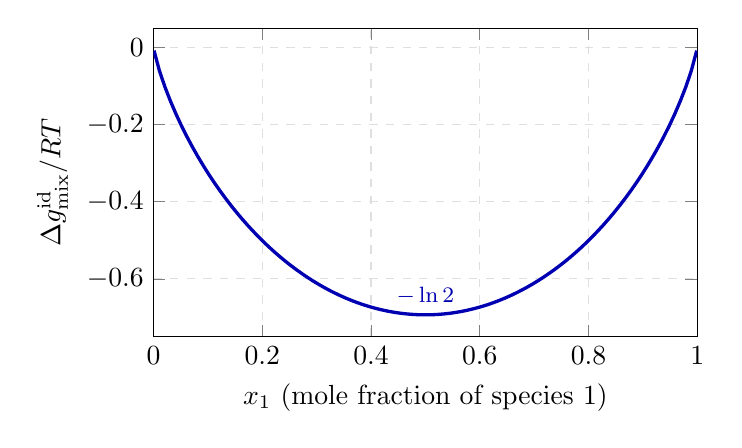
\begin{tikzpicture}
\begin{axis}[
    width=0.7\linewidth, height=5.5cm,
    xlabel={$x_1$ (mole fraction of species 1)},
    ylabel={$\Delta g_{\mathrm{mix}}^{\mathrm{id}} / RT$},
    xmin=0, xmax=1,
    ymin=-0.75, ymax=0.05,
    grid=major,
    grid style={gray!25, dashed},
    every axis title/.style={below=1pt, at={(0.5,1)}, anchor=south},
]
\addplot [domain=0.001:0.999, samples=100, blue!70!black, very thick]
  ({x},{x*ln(x) + (1-x)*ln(1-x)});
\node[anchor=south, font=\footnotesize, text=blue!70!black]
  at (axis cs:0.5, -0.693) {$-\ln 2$};
\end{axis}
\end{tikzpicture}
\caption{Ideal-mixture Gibbs energy of mixing for a binary at fixed
$T$.  Negative everywhere except at the pure-component endpoints
($x_1 = 0$ or $1$, where the curve is tangent to zero with a vertical
slope from the $\ln$ singularity).  The minimum at $x_1 = 0.5$ is
exactly $-RT \ln 2$.}
\label{fig:ideal-gmix}
\end{figure}

\begin{intuition}
The cusps at $x_1 = 0$ and $x_1 = 1$ are characteristic of
combinatorial mixing: an infinitesimal amount of impurity in a pure
liquid produces a finite drop in $g$, because the configurational
entropy gain $-R x \ln x \to +\infty$ as $x \to 0^+$.  This is the
thermodynamic root of why ultra-purification is hard: every
additional decade of purity costs an infinite Gibbs energy.
\end{intuition}

\subsection{Where the ideal limit goes wrong}

Ideal mixing is the right \emph{reference}, not the right
\emph{description}, for most real liquids:

\begin{itemize}[leftmargin=*,nosep]
  \item \textbf{Chemically similar species, weak interactions
        (alkanes, aromatics):} Raoult holds to within 1--5\%.
        Activity coefficients are close to 1; the ideal model is
        useful directly.
  \item \textbf{Polar / non-polar pairs (water with hydrocarbons):}
        $\gamma_i \gg 1$, often $> 10$.  Ideal mixing under-predicts
        the escape tendency of one component in the other by orders
        of magnitude; liquid-liquid splits become possible.
  \item \textbf{Hydrogen-bonded systems (ethanol/water, acid/water):}
        $\gamma_i$ varies smoothly but non-trivially across
        composition; can hit azeotropes (minimum or maximum on the
        bubble curve) that the ideal model cannot represent at all.
  \item \textbf{Strong specific interactions (acid/base, hydrogen-
        bond donors with acceptors):} $\gamma_i < 1$ (negative
        deviations), maximum-boiling azeotropes; again outside the
        ideal-mixture description.
\end{itemize}

The activity coefficient $\gamma_i$ is the multiplicative correction
that puts \eqref{eq:ideal-mu} back on top of the experimental data:
\begin{equation}
   \mu_i(T, P, \mathbf{x})
   \;=\; \mu_i^*(T, P) \;+\; RT \ln(x_i\,\gamma_i)
   \;=\; \mu_i^{\mathrm{id}}(T, P, \mathbf{x}) \;+\; RT \ln \gamma_i.
\end{equation}
The next chapter is about how that correction is parametrised
(NRTL, Wilson) and how the excess Gibbs energy $G^E$ generates
$\gamma_i$ through a partial-derivative recipe.

% ---------------------------------------------------------------------
\section{Activity coefficients}\label{ch:activity}

\begin{whatyoulllearn}
Three models cover the simulator's needs. They share a
common derivation: an expression for excess Gibbs energy $\Gex$ from
which $\gamma_i$ falls out by differentiation.
\end{whatyoulllearn}

\subsection{The excess Gibbs energy bridge}

For a real liquid mixture, the molar Gibbs energy is split as
\begin{equation}
   G^L(T, P, \xv) \;=\; G^{L,\mathrm{ideal}}(T, P, \xv) \;+\; \Gex(T, \xv).
\end{equation}
The activity coefficient is the composition derivative:
\begin{equation}
   \boxed{\;
   \ln \gamma_i \;=\; \frac{1}{\Rgas T}\left(\frac{\partial (n\,\Gex)}{\partial n_i}\right)_{T,P,n_{j \ne i}}
   \;}
   \label{eq:gamma-from-GE}
\end{equation}
Pick a model for $\Gex$, do the derivative, and you have an activity
model. That is what NRTL, Wilson, UNIQUAC and friends are: each is one
choice of $\Gex(\xv, T)$.

\subsection{Ideal solution}

If $\Gex = 0$, then $\gamma_i = 1$ for every component. Raoult's law:
$y_i P = x_i \Psat_i(T)$. Useful as a baseline, a sanity check, and a
starting point for the Wegstein outer loop.

\subsection{NRTL (Renon and Prausnitz, 1968)}\label{sec:nrtl}

The model that earns its keep in this simulator is NRTL --- the
\emph{Non-Random Two-Liquid} model. It is the default for non-ideal
VLE and the engine behind every liquid--liquid split: NRTL is the only
$\Gex$ model in Choupo that can represent demixing, because (unlike
Wilson, \S\ref{sec:wilson-limit}) its denominators admit the
doubly-tangent $\Gex$ shape that two coexisting liquids require.
Everything below is implemented in
\file{src/thermo/activityCoefficient/NRTL.cpp}.

\paragraph{The local-composition idea.}
Renon and Prausnitz's \cite{Renon} starting point --- the same
postulate that underlies Wilson \eqref{eq:wilson-local} --- is that a
real liquid is not randomly mixed. Around a central molecule of type
$i$, the local mole fraction of $j$-neighbours, $x_{ji}$, is biased

\begin{figure}[ht]\centering
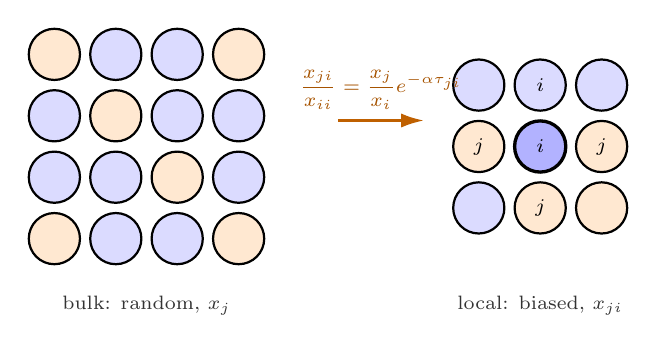
\begin{tikzpicture}[
    >={Latex[width=1.8mm]},
    cell/.style={circle, draw, thick, minimum size=6.5mm, inner sep=0pt,
                 font=\scriptsize},
    A/.style={cell, fill=blue!14},
    B/.style={cell, fill=orange!18},
    cen/.style={cell, very thick, fill=blue!30},
]
% bulk (random) lattice on the left
\begin{scope}[xshift=0cm]
  \foreach \x in {0,1,2,3} \foreach \y in {0,1,2,3} {
     \pgfmathparse{mod(\x+\y,3)==0 ? "B" : "A"}
     \edef\cls{\pgfmathresult}
     \node[\cls] at (0.78*\x,0.78*\y) {};
  }
  \node[font=\scriptsize, text=gray!40!black] at (1.17,-0.85) {bulk: random, $x_j$};
\end{scope}
% local (biased) lattice on the right: a central i with biased neighbour shell
\begin{scope}[xshift=5.0cm]
  \node[cen] (c) at (1.17,1.17) {$i$};
  % nearest shell biased toward j (orange)
  \node[B] at (0.39,1.17) {$j$};
  \node[B] at (1.95,1.17) {$j$};
  \node[B] at (1.17,0.39) {$j$};
  \node[A] at (1.17,1.95) {$i$};
  % corners / outer
  \node[A] at (0.39,0.39) {};
  \node[B] at (1.95,0.39) {};
  \node[A] at (0.39,1.95) {};
  \node[A] at (1.95,1.95) {};
  \node[font=\scriptsize, text=gray!40!black] at (1.17,-0.85)
     {local: biased, $x_{ji}$};
\end{scope}
% the Boltzmann arrow between them
\draw[->, very thick, orange!75!black] (3.6,1.5) -- (4.7,1.5)
   node[midway, above, font=\scriptsize, text=orange!65!black]
   {$\dfrac{x_{ji}}{x_{ii}}=\dfrac{x_j}{x_i}e^{-\alpha\tau_{ji}}$};
\end{tikzpicture}
\caption{The local-composition postulate behind NRTL and Wilson.  In a
\emph{randomly} mixed liquid (left) every molecule's neighbour shell
reflects the bulk fractions $x_j$.  Real mixtures are not random: around
a central molecule $i$, the local fraction of $j$-neighbours $x_{ji}$ is
re-weighted by a Boltzmann factor in the pair-energy difference (right).
NRTL's twist is the extra non-randomness constant $\alpha$ in the
exponent --- $\alpha\to0$ recovers the random regular-solution lattice,
larger $\alpha$ sharpens the local ordering.  Every $\tau_{ij}$ and
$\Lambda_{ij}$ in the activity-coefficient formulas is just this biased
shell, counted.}
\label{fig:local-composition-lattice}
\end{figure}

away from the bulk $x_j$ by the difference in pair energy. NRTL's
distinctive twist is a \emph{two-liquid} Boltzmann weighting that
carries an extra non-randomness factor $\alpha$:
\begin{equation}
   \frac{x_{ji}}{x_{ii}} \;=\;
   \frac{x_j}{x_i}\,
   \exp\!\Bigl[-\alpha_{ji}\,\frac{g_{ji}-g_{ii}}{\Rgas T}\Bigr],
   \label{eq:nrtl-local}
\end{equation}
where $g_{ji}$ is the energy of a $j$--$i$ pair and $\alpha_{ji}$
\emph{quenches} the non-randomness: $\alpha\to\infty$ forces complete

\begin{figure}[ht]\centering
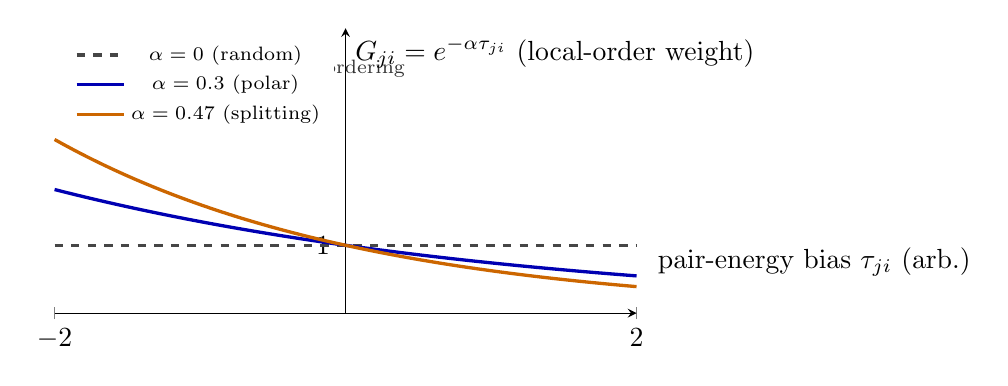
\begin{tikzpicture}
\begin{axis}[
    width=0.74\linewidth, height=5.2cm,
    xlabel={pair-energy bias $\tau_{ji}$ (arb.)},
    ylabel={$G_{ji}=e^{-\alpha\tau_{ji}}$ (local-order weight)},
    ylabel style={align=center},
    xmin=-2, xmax=2, ymin=0, ymax=4.2,
    xtick={-2,0,2}, ytick={1},
    axis lines=middle, clip=false,
    legend style={font=\scriptsize, at={(0.02,0.98)}, anchor=north west, draw=none},
    every axis x label/.style={at={(axis description cs:1.02,0.18)}, anchor=west},
]
\addplot[domain=-2:2, samples=60, gray!55!black, very thick, dashed]
   ({x},{exp(-0.0*x)});
\addlegendentry{$\alpha=0$ (random)}
\addplot[domain=-2:2, samples=60, blue!70!black, very thick]
   ({x},{exp(-0.3*x)});
\addlegendentry{$\alpha=0.3$ (polar)}
\addplot[domain=-2:2, samples=60, orange!80!black, very thick]
   ({x},{exp(-0.47*x)});
\addlegendentry{$\alpha=0.47$ (splitting)}
\node[font=\scriptsize, text=gray!40!black, anchor=west] at (axis cs:-1.9,3.6)
   {larger $\alpha$ $\Rightarrow$ sharper local ordering};
\end{axis}
\end{tikzpicture}
\caption{What the NRTL non-randomness constant $\alpha$ actually does.
The factor $G_{ji}=e^{-\alpha\tau_{ji}}$ is the weight a $j$-neighbour
gets in the shell around an $i$-molecule.  At $\alpha=0$ (flat dashed
line) $G=1$ for every bias --- the shell is random and NRTL collapses to
a regular solution.  Cranking $\alpha$ up steepens the curve, so the same
pair-energy bias $\tau$ produces a sharper deviation of the local shell
from the bulk: $\alpha\approx0.3$ for typical polar mixtures (Choupo's
default when a pair file omits it), $\alpha\approx0.47$ for the strongly
self-associating, phase-splitting systems where the extra ordering is
what carries the liquid--liquid split.  Because $\alpha$ is held fixed
during a fit, a poor choice cannot be repaired by the energy parameters.}
\label{fig:nrtl-alpha-ordering}
\end{figure}

local order, $\alpha=0$ recovers a random (regular-solution) mixture.
In practice $\alpha$ is an adjustable but \emph{transferable} constant,
taken symmetric ($\alpha_{ij}=\alpha_{ji}$) and in the narrow band
$\alpha\in[0.20,\,0.47]$: $\sim\!0.2$ near ideality, $0.3$ for typical
polar mixtures (the simulator's default when a pair file omits it),
$\sim\!0.47$ for strongly self-associating or phase-splitting systems.

\paragraph{The grouped parameters.}
Collecting the two quantities the model actually stores,
\begin{equation}
   \boxed{\;
   \tau_{ij} \;=\; \frac{g_{ij}-g_{jj}}{\Rgas T}
             \;=\; a_{ij} + \frac{b_{ij}}{T}, \qquad
   G_{ij}    \;=\; \exp(-\alpha_{ij}\, \tau_{ij})
   \;}
   \label{eq:nrtl-tauG}
\end{equation}
with the diagonal conventions $\tau_{ii}=0$, $G_{ii}=1$,
$\alpha_{ii}=0$. Two facts matter. First, $\tau$ is \emph{asymmetric}:
$\tau_{ij}\ne\tau_{ji}$ in general, because the energy to place a $j$
next to an $i$ differs from the reverse once each is referenced to its
own pure-fluid pair. Second, the temperature dependence is the affine
form $\tau_{ij}=a_{ij}+b_{ij}/T$ --- exactly the storage in the code:
each ordered pair carries four energy parameters
$(a_{ij},b_{ij},a_{ji},b_{ji})$ and one shared $\alpha_{ij}$ (the
\code{aMat\_}, \code{bMat\_}, \code{alphaMat\_} matrices). Here
$a_{ij}$ is the high-$T$ residual (entropic, temperature-independent)
and $b_{ij}$ [K] is the enthalpic slope. A $b$-only fit ($a=0$) forces
$\tau\to0$ as $T\to\infty$ --- the mixture becomes ideal when thermal
energy swamps the pair energy --- whereas carrying $a\ne0$ admits a
residual that survives.

\paragraph{Excess Gibbs energy.}
Substituting the local compositions \eqref{eq:nrtl-local} into the
two-fluid lattice energy and referencing to the pure components gives
\begin{equation}
   \frac{\Gex}{\Rgas T} \;=\; \sum_{i=1}^{N_c}
       x_i \, \frac{\displaystyle\sum_{j=1}^{N_c} \tau_{ji} G_{ji} x_j}
                  {\displaystyle\sum_{k=1}^{N_c} G_{ki} x_k}.
   \label{eq:nrtl-GE}
\end{equation}

\paragraph{Activity coefficient.}
Apply the partial-molar derivative \eqref{eq:gamma-from-GE}. Write
$n_i = n x_i$ and abbreviate the denominators
$S_j \equiv \sum_k G_{kj} x_k$ (these are \code{S[j]} in the code) and
the numerators $D_j \equiv \sum_k \tau_{kj} G_{kj} x_k$
(\code{Tsum[j]}). Differentiating
$n\Gex/\Rgas T = \sum_i n_i D_i/S_i$ with respect to $n_i$ at fixed
$n_{m\ne i}$ --- using $\partial S_j/\partial n_i = (G_{ij}-S_j)/n$ and
$\partial D_j/\partial n_i = (\tau_{ij}G_{ij}-D_j)/n$ --- the $1/n$
factors cancel and the result is the standard form
\begin{equation}
   \boxed{\;
   \ln \gamma_i \;=\;
   \underbrace{\frac{\displaystyle\sum_j \tau_{ji} G_{ji} x_j}
        {\displaystyle\sum_k G_{ki} x_k}}_{D_i/S_i}
   \;+\;
   \sum_j \frac{x_j G_{ij}}{\;S_j\;}
   \left[\,\tau_{ij} - \frac{D_j}{S_j}\,\right]
   \;}
   \label{eq:nrtl-gamma}
\end{equation}
which is term-for-term the loop in \code{NRTL::gamma()}: \code{termA}
is $D_i/S_i$, \code{termB} accumulates the $j$-sum, and the two are
exponentiated. Pre-computing $S_j$ and $D_j$ once per temperature
(rather than inside every $i,j$ pass) is the only optimisation; the
algebra is otherwise the textbook formula. Check a hand derivation
against Renon and Prausnitz \cite{Renon} or
Reid--Prausnitz--Poling \cite{RPP}, Eq.~8-10.

\begin{intuition}
Read \eqref{eq:nrtl-gamma} as ``the environment $i$ creates plus the
environments $i$ disturbs.'' The first term is how strongly $i$ is held
by its own surroundings; the sum is the back-reaction --- $i$ entering
each cell $j$ and changing its tally. At infinite dilution
($x_i\to0$) the cell of the majority solvent dominates and
$\ln\gamma_i^\infty$ collapses to a closed expression in the pair
parameters --- the quantity most sensitive to a fit.
\end{intuition}

\paragraph{Pairs and the ideal-default rule.}
Binary parameter sets are tabulated in the DECHEMA Vapor--Liquid
Equilibrium Data Collection or regressed from data; the tutorials carry
literature values from Reid--Prausnitz--Poling \cite{RPP}. The
simulator resolves each pair in a fixed precedence
(\code{locatePairFile}): an inline \code{pairs(...)} block in the
\code{thermoPackage}, then a per-node
\file{constant/binaryPairs/NRTL/<a>-<b>.dat}, then the case root, then
\file{data/standards/binaryPairs/NRTL/}. For an $N_c$-component mixture
there are $N_c(N_c-1)/2$ binaries; NRTL is a strictly \emph{pairwise}
model with \emph{no} ternary parameters, so a multicomponent
prediction is only as good as its constituent binaries.

A pair with no parameters anywhere does \emph{not} abort the run: it
\textbf{defaults to ideal} ($\tau=0\Rightarrow$ no $\Gex$ contribution;
$\alpha$ set to $0.3$ harmlessly). This is deliberate --- it lets a
thermo package be built one pair at a time --- but it is never silent:
every ideal-defaulted pair is announced on \code{stdout} and in the
advisory log, so the student \emph{sees} exactly which interactions are
unconstrained. To produce one's own fitted set from a $T_b$-vs-$x$
dataset, run the parameter-estimation driver of Chapter~\ref{ch:lm}
(\file{tutorials/steady/optimisation/fitNRTL01\_ethanol\_water}).

\paragraph{Power.} Two energy parameters per direction plus one
non-randomness constant span ideality, strong positive deviation, and
liquid--liquid immiscibility within a single algebraic form; the affine
$\tau(T)$ extrapolates across a modest temperature range; and the model
is analytically differentiable (used for the bubble-point Jacobian).

\paragraph{Limit.} NRTL is a \emph{fitting} model, not a predictive
one: the parameters have no first-principles values and must come from
data (contrast UNIFAC, which predicts them from group contributions).
It carries no information about the vapour or the solid --- it gives
$\gamma$ for the liquid only; you still supply $\Psat$ from Antoine
(\S\ref{ch:vap}) and any $K_{sp}$ separately. The affine $\tau(T)$ is
calorimetrically uncalibrated unless each pair is refit against
measured $H^E$ (the \code{calorimetricFit} gate that NRTL exposes), so
excess-enthalpy predictions from a VLE-only fit are not to be trusted.
And because $\alpha$ is held fixed during a fit, a poor $\alpha$ choice
cannot be repaired by the energy parameters.

\subsection{Wilson (1964)}\label{sec:wilson}

Simpler in form than NRTL, faster numerically (no $\alpha$, no nested
$G$-exponentials), and built on a more physical picture --- but with one
structural cost: it \emph{cannot represent} a liquid-liquid split. That
is a limitation of the functional form, not of the fit, and the reason
is worth understanding rather than memorising (\S\ref{sec:wilson-limit}).

\paragraph{The idea: local compositions.}
Wilson's \cite{Wilson} starting point is that the composition
\emph{immediately around} a central molecule is not the bulk
composition. If molecule $1$ attracts molecule $2$ more strongly than it
attracts its own kind, then the local mole fraction of $2$ near a $1$ is
enriched above $x_2$. Wilson postulated that these \emph{local} mole
fractions $x_{ji}$ (species $j$ around a central $i$) are related to the
bulk ones through Boltzmann factors of the interaction energies
$\lambda_{ji}$:
\begin{equation}
   \frac{x_{ji}}{x_{ii}}
   \;=\;
   \frac{x_j\,\exp\!\left(-\lambda_{ji}/\Rgas T\right)}
        {x_i\,\exp\!\left(-\lambda_{ii}/\Rgas T\right)} .
   \label{eq:wilson-local}
\end{equation}
Weighting each local environment by the molar volume of the central
species and collecting the result into an excess Gibbs energy yields the
one-line model below. The same local-composition postulate underlies
NRTL and UNIQUAC; Wilson is its earliest and leanest realisation.

\paragraph{Excess Gibbs energy.}
\begin{equation}
   \boxed{\;
   \frac{\Gex}{\Rgas T} \;=\;
   -\sum_{i=1}^{N_c} x_i \ln \!\left(\sum_{j=1}^{N_c} x_j \Lambda_{ij}\right)
   \;}
   \label{eq:wilson-GE}
\end{equation}
with the asymmetric, dimensionless interaction parameter
\begin{equation}
   \Lambda_{ij} \;=\; \frac{V_j^L}{V_i^L}\,
        \exp\!\Bigl[-\underbrace{(\lambda_{ij} - \lambda_{ii})}_{\textstyle A_{ij}}\big/(\Rgas T)\Bigr],
   \qquad \Lambda_{ii} = 1 .
   \label{eq:wilson-Lambda}
\end{equation}
Here $V_i^L$ is the pure-component liquid molar volume and
$\lambda_{ij}$ the energy of an $i$--$j$ interaction. Only the
\emph{difference} $A_{ij} \equiv \lambda_{ij}-\lambda_{ii}$ ever appears,
so Wilson carries \textbf{two} energy parameters per binary, $A_{ij}$ and
$A_{ji}$ (in J/mol), and these are \emph{asymmetric}:
$A_{ij}\ne A_{ji}$ in general, hence $\Lambda_{ij}\ne\Lambda_{ji}$. There
is no third ``non-randomness'' factor as in NRTL.

\paragraph{From $\Gex$ to $\gamma_i$.}
Apply the partial-molar recipe \eqref{eq:gamma-from-GE} to
\eqref{eq:wilson-GE}. Writing $n_i = n x_i$ and
$n\Gex/\Rgas T = -\sum_i n_i \ln\!\big(\sum_j n_j\Lambda_{ij}/n\big)$,
the derivative $\partial/\partial n_i$ contributes one term from the
explicit $\ln$ at $i$ and one from every other molecule's denominator in
which $i$ appears. After re-dividing by $n$ the result collapses to the
classic two-term form:
\begin{equation}
   \boxed{\;
   \ln \gamma_i \;=\;
   1 - \ln\!\left(\sum_{j} x_j \Lambda_{ij}\right)
   \;-\;\sum_{k} \frac{x_k\, \Lambda_{ki}}
                      {\displaystyle\sum_{j} x_j\, \Lambda_{kj}}
   \;}
   \label{eq:wilson-gamma}
\end{equation}
This is exactly the loop in
\file{src/thermo/activityCoefficient/Wilson.cpp}: the code first builds
the $\Lambda$ matrix from \eqref{eq:wilson-Lambda}, precomputes
$S_k=\sum_j x_j\Lambda_{kj}$ once, then assembles
\eqref{eq:wilson-gamma} as $1-\ln S_i - \sum_k x_k\Lambda_{ki}/S_k$.

\paragraph{Built-in consistency.} Two checks fall out for free, and the
code reproduces them. At infinite dilution of $i$ in pure $j$
($x_j\to1$) the second sum keeps only the $k=j$ term, giving the
limiting activity coefficient
\begin{equation}
   \ln\gamma_i^{\infty} \;=\; 1 - \ln\Lambda_{ij} - \Lambda_{ji},
\end{equation}
a convenient handle for fitting to a single $\gamma^{\infty}$ datum. And
in the pure limit $x_i\to1$ every $S_k\to\Lambda_{ki}$ and
\eqref{eq:wilson-gamma} returns $\ln\gamma_i = 1 - \ln 1 - 1 = 0$, i.e.
$\gamma_i\to1$ as it must.

\paragraph{Temperature dependence --- and an honest caveat.}
The $T$-dependence in Choupo's Wilson is \emph{implicit only}, through
the Boltzmann factor $\exp(-A_{ij}/\Rgas T)$ and the (weakly
$T$-varying) volume ratio in \eqref{eq:wilson-Lambda}: the energy
parameters $A_{ij}$ themselves are stored as single constants in J/mol,
not as a $T$-expansion. This is deliberately \emph{unlike} the NRTL
implementation, whose $\tau_{ij}=a_{ij}+b_{ij}/T$
\eqref{eq:nrtl-GE} carries an explicit linear-in-$1/T$ term. If a wider
temperature range demands it, the physically standard refinement is to
let $A_{ij}=A_{ij}^{0}+A_{ij}^{1}\,T$ (a linear-in-$T$ energy, the form
used by DECHEMA for Wilson); that extra slope is not yet wired
into the loader, so over a broad $T$ window prefer a pair fitted near the
operating temperature. The single-constant choice keeps the glass-box
small: one number per direction, visible in the \file{.dat}.

\paragraph{Wilson vs NRTL at a glance.}
\begin{center}
\begin{tabular}{lll}
\hline
                       & \textbf{Wilson} & \textbf{NRTL} \\
\hline
Parameters / binary    & $A_{ij},A_{ji}$ (2)        & $a_{ij},b_{ij},a_{ji},b_{ji},\alpha$ (5) \\
Needs $V_i^L$?         & yes (liquid molar volume)  & no \\
$T$-model in Choupo    & $\exp(-A/\Rgas T)$ only     & explicit $a+b/T$ in $\tau$ \\
Liquid-liquid split    & \textbf{impossible}        & yes (its main strength) \\
Cost per $\gamma$ eval & one $\ln$, one nested sum  & two nested sums + $\exp$ \\
\hline
\end{tabular}
\end{center}

\paragraph{Why Wilson cannot demix.}\label{sec:wilson-limit}
A liquid-liquid split requires $\Gex$ to be non-convex in composition
(a region where $\partial^2 G/\partial x^2 < 0$). For a binary,
$\Gex/\Rgas T = -x_1\ln(x_1+x_2\Lambda_{12})-x_2\ln(x_2+x_1\Lambda_{21})$
is mathematically incapable of producing two minima for any positive

\begin{figure}[ht]\centering
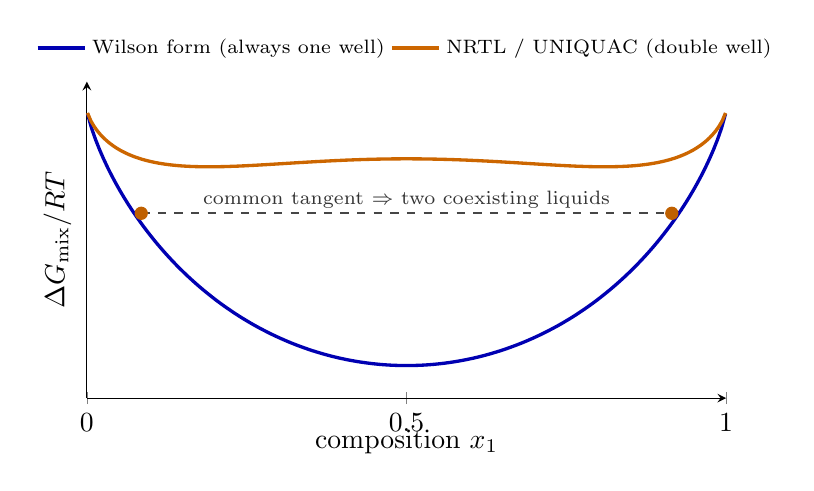
\begin{tikzpicture}
\begin{axis}[
    width=0.80\linewidth, height=5.6cm,
    xlabel={composition $x_1$},
    ylabel={$\Delta G_{\mathrm{mix}}/RT$},
    xmin=0, xmax=1, ymin=-0.40, ymax=0.04,
    xtick={0,0.5,1}, ytick=\empty,
    axis lines=left, clip=false,
    legend style={font=\scriptsize, at={(0.5,1.04)}, anchor=south, draw=none},
    legend columns=2,
    every axis x label/.style={at={(axis description cs:0.5,-0.07)}, anchor=north},
]
% Wilson-like: always convex single well
\addplot[domain=0.001:0.999, samples=160, blue!70!black, very thick]
  ({x}, { 0.62*(x*ln(x)+(1-x)*ln(1-x)) + 0.30*x*(1-x) });
\addlegendentry{Wilson form (always one well)}
% NRTL/UNIQUAC-like: double well (non-convex hump)
\addplot[domain=0.001:0.999, samples=200, orange!80!black, very thick]
  ({x}, { 0.62*(x*ln(x)+(1-x)*ln(1-x)) + 1.45*x*(1-x) });
\addlegendentry{NRTL / UNIQUAC (double well)}
% common tangent marking the two coexisting compositions of the orange curve
\addplot[only marks, mark=*, mark size=2.2pt, mark options={orange!75!black}]
   coordinates {(0.085,-0.143) (0.915,-0.143)};
\draw[dashed, gray!55!black, thick] (axis cs:0.085,-0.143) -- (axis cs:0.915,-0.143);
\node[font=\scriptsize, text=gray!40!black, anchor=south] at (axis cs:0.5,-0.150)
   {common tangent $\Rightarrow$ two coexisting liquids};
\end{axis}
\end{tikzpicture}
\caption{Why the model's \emph{form} --- not its fit --- decides whether
a liquid can split.  A liquid--liquid split needs $\Delta G_{\mathrm{mix}}$
to be non-convex: a hump with two wells, so a common tangent touches two
distinct compositions (the orange curve).  Wilson's single logarithm per
term, $\Gex/RT=-x_1\ln(x_1+x_2\Lambda_{12})-x_2\ln(x_2+x_1\Lambda_{21})$,
is mathematically incapable of producing that hump for any positive
$\Lambda$ --- it stays convex (blue), so no parameter set makes Wilson
demix.  NRTL and UNIQUAC carry the extra freedom for a double well, which
is exactly why Choupo's LLE Gibbs-minimisation accepts those two and
refuses Wilson.}
\label{fig:wilson-vs-nrtl-wells}
\end{figure}

$\Lambda_{12},\Lambda_{21}$ --- the single logarithm per term keeps the
curve convex. No choice of parameters fixes this; it is the price of the
one-parameter-pair-per-direction simplicity. For partially miscible
systems (e.g. the LLE Gibbs-minimisation of Chapter~\ref{ch:lle-gibbs}) the simulator
falls back to NRTL or UNIQUAC, which carry the extra freedom needed for a
double-well $\Gex$.

\paragraph{Parameter sources.} Binary $(A_{ij},A_{ji})$ sets live in
\file{data/standards/binaryPairs/Wilson/<i>-<j>.dat} (or a case-local
\file{constant/binaryPairs/Wilson/}); a pair with no file anywhere
\emph{defaults to ideal} for that binary ($\Lambda=1$, no contribution)
and the run announces it aloud rather than aborting --- the same
no-silent-crutch hybrid used by NRTL. Literature values are tabulated in
the DECHEMA collection and Reid--Prausnitz--Poling \cite{RPP}; fit your
own with the parameter-estimation driver of Chapter~\ref{ch:lm}.

\begin{example}[Wilson $\gamma$ for ethanol(1)/water(2) at 350\,K, $x_1=0.20$]
Parameters $A_{12}=1157.95$, $A_{21}=4081.65$\,J/mol (the values shipped
in the \file{ethanol-water.dat} Wilson pair) and liquid molar volumes
$V_1^L=5.87\times10^{-5}$, $V_2^L=1.81\times10^{-5}$\,m$^3$/mol. With
$\Rgas T = 8.314\times350 = 2910$\,J/mol:
\[
   \Lambda_{12}=\tfrac{V_2}{V_1}e^{-A_{12}/\Rgas T}
              =\tfrac{1.81}{5.87}\,e^{-0.398}=0.207,\quad
   \Lambda_{21}=\tfrac{V_1}{V_2}e^{-A_{21}/\Rgas T}
              =\tfrac{5.87}{1.81}\,e^{-1.403}=0.797 .
\]
At $x_1=0.20$: $S_1=x_1+x_2\Lambda_{12}=0.20+0.80(0.207)=0.366$ and
$S_2=x_2+x_1\Lambda_{21}=0.80+0.20(0.797)=0.959$. Then from
\eqref{eq:wilson-gamma},
\[
   \ln\gamma_1 = 1 - \ln 0.366
     - \!\left[\frac{x_1\Lambda_{11}}{S_1}+\frac{x_2\Lambda_{21}}{S_2}\right]
   = 1 - (-1.005) - \!\left[\tfrac{0.20}{0.366}+\tfrac{0.80\cdot0.797}{0.959}\right]
   \approx 0.84,
\]
so $\gamma_1\approx2.3$. Ethanol is strongly non-ideal here --- the same
qualitative verdict as the NRTL example above, with a different model and
two fewer parameters.
\end{example}

\subsection{UNIQUAC (Abrams and Prausnitz, 1975)}\label{sec:uniquac}

\begin{figure}[ht]\centering
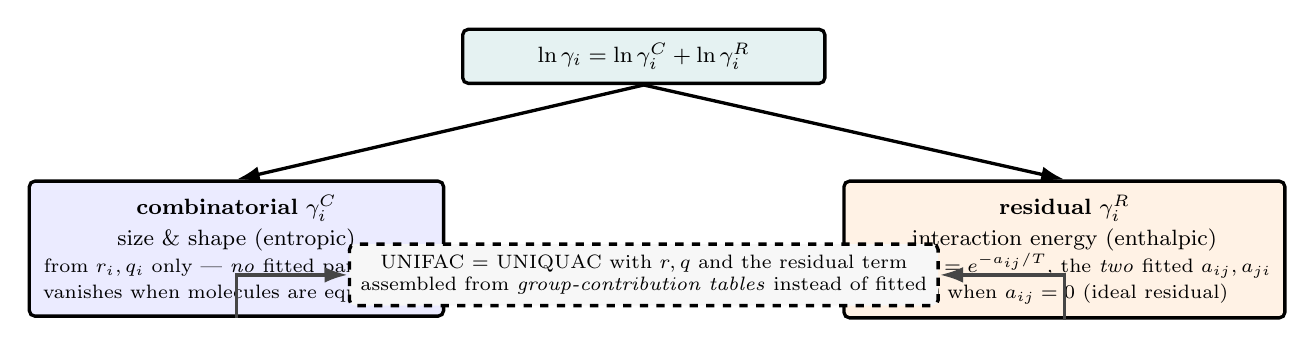
\begin{tikzpicture}[
    >={Latex[width=2.0mm]},
    top/.style ={draw, rounded corners=2pt, very thick, align=center,
                 inner sep=5pt, minimum width=46mm, font=\footnotesize,
                 fill=teal!10},
    comb/.style={draw, rounded corners=2pt, very thick, align=center,
                 inner sep=5pt, minimum width=44mm, font=\footnotesize,
                 fill=blue!8},
    res/.style ={draw, rounded corners=2pt, very thick, align=center,
                 inner sep=5pt, minimum width=44mm, font=\footnotesize,
                 fill=orange!10},
    flow/.style={->, very thick},
]
\node[top] (sum) {$\ln\gamma_i=\ln\gamma_i^{C}+\ln\gamma_i^{R}$};
\node[comb, below left=12mm and 2mm of sum] (c)
  {\textbf{combinatorial} $\gamma_i^{C}$\\[2pt]
   size \& shape (entropic)\\
   {\scriptsize from $r_i,q_i$ only --- \emph{no} fitted parameters}\\
   {\scriptsize vanishes when molecules are equal-sized}};
\node[res, below right=12mm and 2mm of sum] (r)
  {\textbf{residual} $\gamma_i^{R}$\\[2pt]
   interaction energy (enthalpic)\\
   {\scriptsize from $\tau_{ij}=e^{-a_{ij}/T}$, the \emph{two} fitted $a_{ij},a_{ji}$}\\
   {\scriptsize $\to0$ when $a_{ij}=0$ (ideal residual)}};
\draw[flow] (sum.south) -- (c.north);
\draw[flow] (sum.south) -- (r.north);
% the UNIFAC link
\node[draw, dashed, very thick, rounded corners=2pt, below=20mm of sum,
      align=center, inner sep=4pt, font=\scriptsize, fill=gray!6,
      minimum width=70mm] (unifac)
  {UNIFAC $=$ UNIQUAC with $r,q$ and the residual term\\
   assembled from \emph{group-contribution tables} instead of fitted};
\draw[flow, gray!55!black] (c.south) |- (unifac.west);
\draw[flow, gray!55!black] (r.south) |- (unifac.east);
\end{tikzpicture}
\caption{UNIQUAC's defining move: split the excess Gibbs energy into two
physically distinct pieces.  The \textbf{combinatorial} term (blue)
carries the entropic penalty of packing molecules of unequal size and
shape --- it needs only the structural constants $r_i,q_i$ and has
\emph{zero} fitted parameters, vanishing entirely when all molecules are
the same size.  The \textbf{residual} term (orange) carries the
interaction energy through $\tau_{ij}=e^{-a_{ij}/T}$ and holds the
\emph{two} binary energies $(a_{ij},a_{ji})$ --- one fewer than NRTL,
which also needs $\alpha$.  Because the size/shape physics lives in $r,q$,
this is the exact structure UNIFAC reuses: keep the combinatorial term as
is and build the residual from group-contribution tables instead of a
binary fit.}
\label{fig:uniquac-two-term-split}
\end{figure}


NRTL and Wilson are \emph{energy-only} models: they describe
non-ideality through interaction parameters and quietly assume the
molecules are the same size and shape. That assumption frays for
mixtures of very unequal molecules --- a polymer in a solvent, a sugar
in water, an alkane in an alcohol --- where much of the deviation from
ideality is \emph{entropic}, born of the difficulty of packing big and
small molecules onto a common lattice. UNIQUAC (UNIversal QUAsi-Chemical)
\cite{Abrams1975} splits the excess Gibbs energy into two physically
distinct pieces and gives each its own term:
\begin{equation}
   \frac{\Gex}{\Rgas T}
   \;=\;
   \underbrace{\frac{\Gex_{\mathrm{comb}}}{\Rgas T}}_{\text{size/shape (entropic)}}
   \;+\;
   \underbrace{\frac{\Gex_{\mathrm{res}}}{\Rgas T}}_{\text{energy (enthalpic)}},
   \qquad\Longrightarrow\qquad
   \ln \gamma_i \;=\; \ln \gamma_i^{C} + \ln \gamma_i^{R}.
   \label{eq:uniquac-split}
\end{equation}
The \emph{combinatorial} part $\gamma_i^{C}$ depends only on
\emph{structural} constants; the \emph{residual} part $\gamma_i^{R}$
carries the two adjustable binary energies. This is exactly the
structure that lets UNIFAC \emph{predict} $\gamma$ from group counts:
UNIFAC is UNIQUAC with $r$, $q$ and the residual term assembled from
group-contribution tables instead of being fitted.

\paragraph{Structural constants.} Each component carries two
pure-component numbers, computed from its van der Waals group volumes and
surface areas (Bondi, 1968):
\begin{equation}
   r_i \;=\; \text{relative molecular \emph{volume}}, \qquad
   q_i \;=\; \text{relative molecular \emph{surface area}}.
\end{equation}
These are not fitted --- they are tabulated constants the student
\emph{cites} (Poling--Prausnitz--O'Connell \cite{RPP}, Table 8E;
original values in \cite{Abrams1975}). In the dict they live in an
\code{rq \{ \dots \}} block, one $\{r;\,q;\}$ pair per component; the
engine refuses to run if any is missing (no silent default for a
structural property). From $r$ and $q$ the model builds, at a given
composition, the \emph{segment fraction} $\phi_i$ and \emph{area
fraction} $\theta_i$:
\begin{equation}
   \phi_i \;=\; \frac{r_i x_i}{\displaystyle\sum_j r_j x_j}, \qquad
   \theta_i \;=\; \frac{q_i x_i}{\displaystyle\sum_j q_j x_j}.
   \label{eq:uniquac-fractions}
\end{equation}
Two limits aid intuition: if all $r_i$ are equal then $\phi_i = x_i$,
and if additionally all $q_i$ are equal then $\theta_i = x_i$ and the
combinatorial term vanishes --- equal-sized molecules carry no packing
penalty.

\paragraph{Combinatorial (size/shape) term.} The entropic piece is a
Staverman--Guggenheim lattice count, with activity coefficient
\begin{equation}
   \ln \gamma_i^{C}
   \;=\;
   \ln\!\frac{\phi_i}{x_i}
   \;+\; \frac{z}{2}\, q_i \ln\!\frac{\theta_i}{\phi_i}
   \;+\; l_i
   \;-\; \frac{\phi_i}{x_i}\sum_{j} x_j l_j,
   \qquad
   l_i \;=\; \frac{z}{2}(r_i - q_i) - (r_i - 1),
   \label{eq:uniquac-comb}
\end{equation}
where the \emph{lattice coordination number} is fixed at $z = 10$ (each
molecule is taken to have ten nearest neighbours --- the canonical
UNIQUAC value, hard-coded as \code{z\_coord\_} in the engine, not a
tunable). This term contains \emph{no} adjustable parameters: feed it the
$r$'s and $q$'s and it is fully determined. It alone already predicts the
bulk of athermal (zero-energy) non-ideality.

\paragraph{Residual (energy) term.} The enthalpic piece uses the
\emph{quasi-chemical} idea --- a molecule's surroundings are biased by
interaction energies through Boltzmann factors
\begin{equation}
   \tau_{ij} \;=\; \exp\!\Bigl(-\frac{u_{ij} - u_{jj}}{\Rgas T}\Bigr)
              \;=\; \exp\!\Bigl(-\frac{a_{ij}}{T}\Bigr),
   \qquad
   a_{ij} \;=\; \frac{u_{ij} - u_{jj}}{\Rgas}\ \ [\mathrm{K}],
   \label{eq:uniquac-tau}
\end{equation}
with $u_{ij}$ the $i$--$j$ interaction energy. Note $\tau_{ii} = 1$ and
the matrix is asymmetric ($\tau_{ij}\neq\tau_{ji}$); each binary
contributes \emph{two} energies $a_{ij}, a_{ji}$ --- one fewer than NRTL,
which also needs $\alpha$. The engine stores $a_{ij}$ in \emph{kelvin}
and supports an optional linear extension
$a^{\mathrm{eff}}_{ij} = a_{ij} + b_{ij}\,T$ for sets fitted over a wide
temperature range (most literature sets use $a$ alone, $b=0$). The
residual activity coefficient is
\begin{equation}
   \ln \gamma_i^{R}
   \;=\;
   q_i\left[\,1
   - \ln\!\Bigl(\sum_{j}\theta_j \tau_{ji}\Bigr)
   - \sum_{j}\frac{\theta_j \tau_{ij}}
                   {\displaystyle\sum_{k}\theta_k \tau_{kj}}
   \,\right].
   \label{eq:uniquac-res}
\end{equation}
Equations \eqref{eq:uniquac-comb} and \eqref{eq:uniquac-res} are exactly
what \file{src/thermo/activityCoefficient/UNIQUAC.cpp} evaluates in
\code{gamma()} --- read the two side by side.

\paragraph{Parameter sources and the ideal default.} The two energies
$(a_{ij}, a_{ji})$ per binary come from VLE regression (DECHEMA, or the
parameter-estimation driver of Chapter~\ref{ch:lm}), supplied inline as
\code{pairs (\dots)} or from a UNIQUAC pair catalogue
(\file{constant/binaryPairs/UNIQUAC/<a>-<b>.dat}, the same precedence
NRTL and Wilson use). A binary with no parameters anywhere defaults to
$a_{ij}=a_{ji}=0$, i.e.\ $\tau=1$ (ideal residual contribution), and the
run \emph{announces} the defaulted pairs aloud --- the same
no-silent-crutch hybrid as NRTL and Wilson.

\paragraph{Power and limit.}
UNIQUAC needs only \emph{two} energy parameters per binary (vs three for
NRTL) yet, because the size/shape physics is built in through $r$ and
$q$, it extrapolates over composition and to multicomponent mixtures
better than NRTL or Wilson for molecules of disparate size. Unlike Wilson
it \emph{can} describe liquid--liquid demixing (its $\Gex$ admits a
double well), so the LLE Gibbs-minimisation of
Chapter~\ref{ch:lle-gibbs} accepts it alongside NRTL. And it is the
structural parent of UNIFAC, so a UNIQUAC \emph{fit} and a UNIFAC
\emph{prediction} are directly comparable on the same components. The
\textbf{limit}: the two-parameter residual term is less flexible than
NRTL's three-parameter form for a single tightly-fitted binary --- for a
strongly hydrogen-bonded pair fitted on its own data NRTL often edges it.
The combinatorial term is a mean-field lattice count that sees molecular
shape only through the single number $q$, so it is imperfect for very
flat or branched species. And, like every $\Gex$ model, it is silent
about the vapour ($\varphi^{\mathrm{sat}}=1$ here) and about ions (use
eNRTL/Pitzer, \S\ref{ch:electrolytes}).

\begin{example}[UNIQUAC $\gamma$ for ethanol(1)/water(2) at $351$\,K, $x_1=0.20$]
The \file{tutorials/steady/flash/bubbleT02\_uniquac\_ethanol\_water}
system. Structural constants $r_1=2.1055,\ q_1=1.9720,\ r_2=0.9200,\
q_2=1.4000$; energies $a_{12}=-21.44\,$K, $a_{21}=222.47\,$K.

\emph{Step 1 --- $\tau$ at $T=351\,$K} (Eq.~\ref{eq:uniquac-tau}):
$\tau_{12}=e^{21.44/351}=1.063$, $\tau_{21}=e^{-222.47/351}=0.531$
(and $\tau_{11}=\tau_{22}=1$).

\emph{Step 2 --- fractions} (Eq.~\ref{eq:uniquac-fractions}) at
$x=(0.20,0.80)$: $\sum r_jx_j = 1.157$, $\sum q_jx_j = 1.514$, hence
$\phi_1=0.364,\ \theta_1=0.260$ (and $\phi_2=0.636,\ \theta_2=0.740$).

\emph{Step 3 --- combinatorial} (Eq.~\ref{eq:uniquac-comb}) with $z=10$:
$l_1=5(2.1055-1.9720)-(2.1055-1)=-0.438$, $l_2=-2.320$,
$\sum x_j l_j = -1.944$, giving $\ln\gamma_1^{C}=0.398$.

\emph{Step 4 --- residual} (Eq.~\ref{eq:uniquac-res}):
$\sum_j\theta_j\tau_{j1}=0.260+0.740(0.531)=0.653$, the second sum
evaluates to $0.247$, so
$\ln\gamma_1^{R}=1.972\,[\,1-\ln 0.653 - 0.247\,]=0.501$.

\emph{Result:} $\ln\gamma_1 = 0.398+0.501=0.899 \Rightarrow
\gamma_1\approx 2.46$ (and $\gamma_2\approx 1.12$). Driving $x_1\to 0$
gives the infinite-dilution value $\gamma_1^{\infty}\approx 7.7$ --- the
strongly-non-ideal range that makes ethanol/water a minimum-boiling
azeotrope, and the very value the tutorial's \file{thermoPackage} energies
were fitted to reproduce.
\end{example}

\begin{tutoriallink}
\file{tutorials/steady/flash/bubbleT02\_uniquac\_ethanol\_water} --- the
bubble temperature of 30/70 ethanol/water at 1\,atm, landing on the same
$T_{\mathrm{bubble}}\approx 354\,$K as its NRTL and Wilson twins: a clean
three-way model comparison on identical components.
\end{tutoriallink}

\subsection{Worked example}

\begin{example}[NRTL $\gamma$ for ethanol/water at 350\,K, $x_1 = 0.20$]
Components $1=$ethanol, $2=$water. Literature parameters (the same set
carried in \file{data/standards/binaryPairs/NRTL/ethanol-water.dat},
from \cite{RPP}):
$a_{12} = -0.8009,\ b_{12} = 246.18\,\mathrm{K},\ a_{21} = 3.4578,\
b_{21} = -586.0809\,\mathrm{K},\ \alpha = 0.30$.

\emph{Step 1 --- $\tau$ and $G$ at $T = 350\,$K} from
\eqref{eq:nrtl-tauG}:
\[
\tau_{12} = -0.8009 + \tfrac{246.18}{350} = -0.0975, \quad
\tau_{21} =  3.4578 - \tfrac{586.08}{350} = \phantom{-}1.7833,
\]
\[
G_{12} = e^{-0.3(-0.0975)} = 1.0297, \quad
G_{21} = e^{-0.3(1.7833)}  = 0.5857.
\]

\emph{Step 2 --- the binary $\ln\gamma_1$.} For two components
\eqref{eq:nrtl-gamma} reduces to a two-term sum
($\tau_{11}=\tau_{22}=0$, $G_{11}=G_{22}=1$). With $x_1=0.20$,
$x_2=0.80$ the denominators are
$S_1 = x_1 + G_{21}x_2 = 0.20 + 0.5857(0.80) = 0.6686$ and
$S_2 = G_{12}x_1 + x_2 = 1.0297(0.20) + 0.80 = 1.0059$, so
\[
\ln\gamma_1
= \frac{\tau_{21}G_{21}x_2}{S_1}
+ \frac{x_2 G_{12}}{S_2}\!\left[\tau_{12}-\frac{\tau_{12}G_{12}x_1}{S_2}\right]
= 1.250 + (-0.063) = 1.186,
\]
giving $\gamma_1 \approx 3.27$.

\emph{Step 3 --- read it.} Ethanol is strongly non-ideal at this
dilute composition; Raoult's law ($\gamma_1=1$) would under-predict the
ethanol partial pressure threefold. Pushing $x_1\to0$ in the same
formula gives the infinite-dilution value $\gamma_1^\infty \approx 5.4$
--- the steepest, most fit-sensitive point of the curve. At the other
end the same parameters place the well-known minimum-boiling azeotrope
near $x_1 \approx 0.894$, where $\gamma_1\approx\gamma_2 P^{\text{sat}}$
balance crosses (\file{tutorials/batch/still/still02\_ethanol\_water\_azeo}).
\end{example}

\begin{tutoriallink}
\file{tutorials/steady/flash/flash02\_ethanol\_water} --- watch the
Wegstein outer loop converge in $\sim$7 iterations vs $\sim$29 by direct
substitution.
\end{tutoriallink}

% ---------------------------------------------------------------------
\subsection{UNIFAC: predicting $\gamma_i$ from molecular
structure}\label{sec:unifac}

NRTL and Wilson are \emph{correlative}: they reproduce a binary's
non-ideality only after someone has fitted $(a_{ij}, b_{ij}, \alpha)$ or
$(A_{ij}, A_{ji})$ to measured VLE for \emph{that pair}. Confront them
with a binary no one has measured and they have nothing to say. UNIFAC
(\textbf{UNI}QUAC \textbf{F}unctional-group \textbf{A}ctivity
\textbf{C}oefficients) is \emph{predictive}: it computes $\gamma_i(T,
\xv)$ from the \emph{functional groups} that make up each molecule, using
one published parameter table shared across all of chemistry. No binary
fit. The headline glass-box win is to predict the ethanol--water
azeotrope from structure alone and then \emph{see} the residual error
against data. UNIFAC is the group-contribution realisation of UNIQUAC
\cite{Fredenslund1975, RPP}.

\paragraph{The central idea: a solution of groups.} A molecule is
decomposed into a multiset of \emph{subgroups} (e.g.\ ethanol $=$ 1

\begin{figure}[ht]\centering
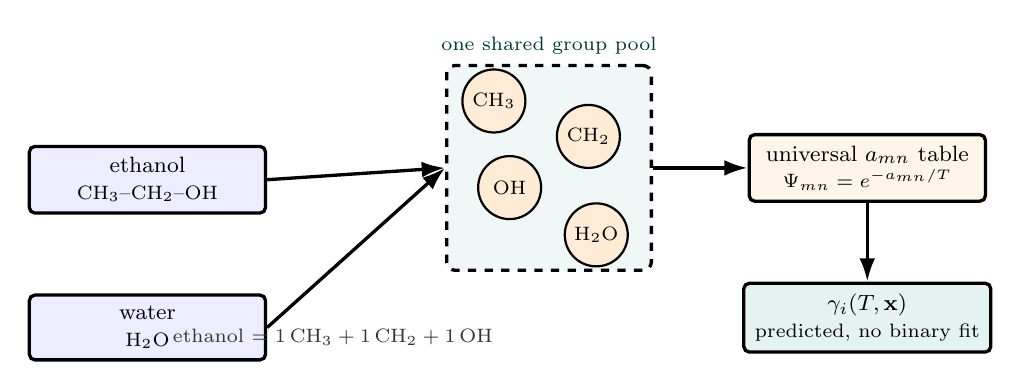
\begin{tikzpicture}[
    >={Latex[width=2.0mm]},
    mol/.style ={draw, rounded corners=2pt, very thick, align=center,
                 inner sep=4pt, minimum width=30mm, font=\footnotesize,
                 fill=blue!7},
    grp/.style ={draw, circle, thick, inner sep=1pt, minimum size=8mm,
                 font=\scriptsize, fill=orange!16},
    pool/.style={draw, rounded corners=3pt, very thick, dashed,
                 inner sep=6pt, fill=teal!6},
    flow/.style={->, very thick},
]
% molecules
\node[mol] (etoh)  {ethanol\\{\scriptsize CH$_3$--CH$_2$--OH}};
\node[mol, below=10mm of etoh] (water) {water\\{\scriptsize H$_2$O}};
% group pool box (explicit rectangle, avoids fit dependency)
\node[pool, minimum width=26mm, minimum height=26mm] (poolbox) at (5.1,0.15) {};
% group pool members placed inside the box
\node[grp] (g1) at (4.4,1.0) {CH$_3$};
\node[grp] (g2) at (5.6,0.55) {CH$_2$};
\node[grp] (g3) at (4.6,-0.1) {OH};
\node[grp] (g4) at (5.7,-0.7) {H$_2$O};
\node[font=\scriptsize, text=teal!45!black, anchor=south]
   at (poolbox.north) {one shared group pool};
% interaction matrix box
\node[mol, right=12mm of poolbox, fill=orange!8] (amat)
   {universal $a_{mn}$ table\\{\scriptsize $\Psi_{mn}=e^{-a_{mn}/T}$}};
% result
\node[mol, below=10mm of amat, fill=teal!10] (gam)
   {$\gamma_i(T,\xv)$\\{\scriptsize predicted, no binary fit}};
\draw[flow] (etoh.east)  -- (poolbox.west);
\draw[flow] (water.east) -- (poolbox.west);
\draw[flow] (poolbox.east) -- (amat.west);
\draw[flow] (amat.south) -- (gam.north);
% counts annotation
\node[font=\scriptsize, text=gray!40!black, anchor=west] at (0.2,-2.0)
   {ethanol $=1\,$CH$_3+1\,$CH$_2+1\,$OH};
\end{tikzpicture}
\caption{UNIFAC's central idea, drawn: a molecule is dissolved into a
\emph{multiset of functional groups} (ethanol $=$ CH$_3+$CH$_2+$OH), and
the mixture is treated as a solution of those groups rather than of
molecules.  A CH$_2$ is assumed to interact with H$_2$O the same way in
every molecule it appears in --- the group-additivity hypothesis --- so a
\emph{single universal} $a_{mn}$ table ($\Psi_{mn}=e^{-a_{mn}/T}$) serves
all of chemistry.  That is what turns UNIQUAC's \emph{fitted} residual
term into a \emph{prediction}: feed in the group counts and out comes
$\gamma_i(T,\xv)$ for a binary nobody ever measured.  The price is
proximity effects and isomers the group count cannot see (see the
limits).}
\label{fig:unifac-group-decomposition}
\end{figure}

\code{CH3} $+$ 1 \code{CH2} $+$ 1 \code{OH}). The mixture is then treated
as a solution not of molecules but of those groups. A \code{CH2} in
ethanol is assumed to interact with a \code{H2O} exactly as a \code{CH2}
in any other molecule would --- the \emph{group-additivity hypothesis}.
This is what lets one parameter matrix (group $m$ against group $n$)
serve every conceivable molecule built from those groups.

\paragraph{Two-part structure.} As in UNIQUAC, the activity coefficient
splits into a size/shape (entropic) part and an energetic part:
\begin{equation}
   \ln \gamma_i \;=\; \underbrace{\ln \gamma_i^{C}}_{\text{combinatorial}}
                \;+\; \underbrace{\ln \gamma_i^{R}}_{\text{residual}}.
   \label{eq:unifac-split}
\end{equation}

\paragraph{Group constants.} Each subgroup $k$ carries a van der Waals
volume $R_k$ and surface area $Q_k$ (tabulated, $T$-independent). Summing
over the $\nu^{(i)}_k$ groups in molecule $i$ gives its molecular volume
and surface parameters
\begin{equation}
   r_i = \sum_k \nu^{(i)}_k R_k,
   \qquad
   q_i = \sum_k \nu^{(i)}_k Q_k.
   \label{eq:unifac-rq}
\end{equation}
These are exactly the UNIQUAC $r_i, q_i$, which is why UNIFAC and
UNIQUAC share the combinatorial term. In the simulator $R_k, Q_k$ live
in \file{data/standards/unifac/groups.dat} (Hansen \emph{et al.}
\cite{Hansen1991}, open-literature original-UNIFAC values).

\paragraph{Combinatorial term (Staverman--Guggenheim).} Purely
geometric --- it depends on $r_i, q_i$ only, never on temperature:
\begin{equation}
   \ln \gamma_i^{C}
   = \ln\frac{\phi_i}{x_i}
    + \frac{Z}{2}\,q_i \ln\frac{\theta_i}{\phi_i}
    + l_i - \frac{\phi_i}{x_i}\sum_j x_j l_j,
   \label{eq:unifac-comb}
\end{equation}
with the volume and surface-area fractions
\begin{equation}
   \phi_i = \frac{r_i x_i}{\sum_j r_j x_j},\qquad
   \theta_i = \frac{q_i x_i}{\sum_j q_j x_j},\qquad
   l_i = \frac{Z}{2}(r_i - q_i) - (r_i - 1),
\end{equation}
and lattice coordination number $Z = 10$. This term alone already
captures the entropic non-ideality of mixing molecules of unequal size
(it is what the Flory--Huggins correction does for polymers). In the code
the quantity actually stored is $l_i$; $\phi_i/x_i$ and $\theta_i/\phi_i$
are formed directly from the running sums $\sum_j r_j x_j$ and
$\sum_j q_j x_j$.

\paragraph{Residual term: $\Gamma_k$ on two scales.} The energetic part
is the difference between how each group ``feels'' in the mixture versus
in the pure component:
\begin{equation}
   \ln \gamma_i^{R}
   \;=\; \sum_k \nu^{(i)}_k
        \bigl[\,\ln \Gamma_k - \ln \Gamma_k^{(i)}\,\bigr],
   \label{eq:unifac-res}
\end{equation}
where $\Gamma_k$ is the residual activity coefficient of group $k$ in the
actual mixture, and $\Gamma_k^{(i)}$ is the \emph{same} group's residual
activity in a reference solution containing only the groups of pure
component $i$. The subtraction is what enforces $\gamma_i \to 1$ as
$x_i \to 1$: a group surrounded by its own molecule has
$\Gamma_k = \Gamma_k^{(i)}$, so the bracket vanishes. Both scales use the
identical functional form:
\begin{equation}
   \ln \Gamma_k = Q_k
   \left[\,1 - \ln\!\Bigl(\sum_m \Theta_m \Psi_{mk}\Bigr)
        - \sum_m \frac{\Theta_m \Psi_{km}}
                       {\sum_n \Theta_n \Psi_{nm}}\,\right],
   \label{eq:unifac-Gamma}
\end{equation}
with the group surface fraction and the group-interaction Boltzmann
factor
\begin{equation}
   \Theta_m = \frac{Q_m X_m}{\sum_n Q_n X_n},
   \qquad
   \Psi_{mn} = \exp\!\left(-\frac{a_{mn}}{T}\right).
   \label{eq:unifac-theta-psi}
\end{equation}
$X_m$ is the mole fraction of group $m$ over all groups in the relevant
solution. The \emph{main-group} interaction parameter $a_{mn}$ [K] is
asymmetric ($a_{mn} \ne a_{nm}$); groups in the same main group have
$a_{mn} = 0$ (so $\Psi_{mn} = 1$). These are the only adjustable numbers
in the whole model, and they are \emph{universal}, not per-binary ---
\file{data/standards/unifac/interactions.dat} (Hansen \emph{et al.}
\cite{Hansen1991}). The implementation in
\file{src/thermo/activityCoefficient/UNIFAC.cpp} uses this
single-parameter $a_{mn}$ (original UNIFAC); the later
temperature-extended form $\Psi_{mn} = \exp[-(a_{mn} + b_{mn}T +
c_{mn}T^2)/T]$ of modified UNIFAC (Dortmund) is \emph{not} implemented.

\paragraph{Subgroups vs.\ main groups.} A subtle but load-bearing point:
$\Psi_{mn}$ is indexed by \emph{main group}, while $R_k, Q_k$ and the
group counting use the \emph{subgroup}. Subgroups sharing a main group
(e.g.\ \code{CH3}, \code{CH2}, \code{CH} all in main group \code{CH2})
have distinct $R_k, Q_k$ but \emph{share} every interaction parameter.
That is how UNIFAC keeps the $a$-matrix small while still telling a
methyl apart from a methylene by size.

\paragraph{The algorithm (glass-box).} For each component $i$ the code:
(1) builds $r_i, q_i, l_i$ from the declared groups
\eqref{eq:unifac-rq}; (2) evaluates the combinatorial term
\eqref{eq:unifac-comb} from the mixture composition; (3) computes
$\ln \Gamma_k$ once for the \emph{mixture} group composition and once for
each \emph{pure}-component group composition $X^{(i)}$ via
\eqref{eq:unifac-Gamma}; (4) assembles the residual
\eqref{eq:unifac-res}; (5) returns $\gamma_i = \exp(\ln\gamma_i^C +
\ln\gamma_i^R)$. The pure-component $\Gamma_k^{(i)}$ are temperature
dependent (through $\Psi$), so they are recomputed at every call rather
than cached. The author declares each component's groups in the
\code{activityModel} block: \code{model UNIFAC;} then a
\code{groups\{\dots\}} sub-dict listing \code{group}/\code{count} per
component. A component absent from \code{groups} falls back to
$\gamma_i = 1$ and logs the gap (no silent crutch).

\begin{example}[Decomposing acetone $+$ $n$-hexane]
Acetone $=$ 1 \code{CH3CO} $+$ 1 \code{CH3}; $n$-hexane $=$ 2 \code{CH3}
$+$ 4 \code{CH2}. With the tabulated $R_{\mathrm{CH3}} = 0.9011,\
Q_{\mathrm{CH3}} = 0.848$ and $R_{\mathrm{CH2}} = 0.6744,\
Q_{\mathrm{CH2}} = 0.540$, hexane gets
$r = 2(0.9011) + 4(0.6744) = 4.500$ and
$q = 2(0.848) + 4(0.540) = 3.856$ from \eqref{eq:unifac-rq} alone ---
no fitting, no data. The non-zero $a_{mn}$ between main groups
\code{CH2CO} and \code{CH2} then drives the group $\Gamma_k$ apart in the
residual term and predicts the strong positive deviations (and the
homogeneous azeotrope) of this notoriously non-ideal pair. Compare the
prediction against the measured Txy through the validation weapon
(Chapter~\ref{ch:lm}) --- that overlay, prediction vs.\ data, is the
whole pedagogical point.
\end{example}

\paragraph{Power.} A genuine prediction --- $\gamma_i$ for an
\emph{unmeasured} binary, even an azeotrope, from structure and a single
universal table. Indispensable when no fitted NRTL/Wilson set exists, and
the natural default when screening many candidate solvents at once.

\paragraph{Limit.} (1) \emph{Only as good as the group table.} A missing
$a_{mn}$ pair is silently treated as $a_{mn} = 0$ (ideal between those
groups) --- the header of \file{interactions.dat} flags this as a known
honesty gap, and a declared group with no $a$-rows yields an unreliable
$\gamma$. (2) \emph{Group-additivity breaks for proximity effects} ---
neighbouring polar groups, intramolecular hydrogen bonds, and isomers the
group count cannot distinguish (UNIFAC sees no difference between two
positional isomers with the same groups). (3) \emph{Weak near a mixture's
critical region and for strongly dilute or asymmetric systems}, and the
original-UNIFAC $\Psi = \exp(-a/T)$ gives only a crude temperature trend
(the reason modified UNIFAC was developed). (4) \emph{No liquid--liquid
split} from this code path; UNIFAC-LLE uses a separate parameter table
not bundled here. The standing lesson: a prediction to be \emph{checked
against data}, never trusted blind --- if you \emph{have} measured VLE for
the pair, a fitted NRTL will beat UNIFAC, and UNIFAC's value is precisely
when you do not.

\section{Electrolyte solutions: ionic strength, the osmotic
coefficient, and Pitzer}\label{ch:electrolytes}

\begin{whatyoulllearn}
A dissolved salt does not obey Raoult's law and does not have a
meaningful vapour pressure, yet it governs the single most important
number in reverse osmosis: the \emph{osmotic pressure} $\pi$, the
hydraulic head a membrane must overcome before a drop of water will
cross.  This chapter builds $\pi$ from first principles --- the
equality of solvent chemical potential across the membrane --- arrives
at the ideal-dilute \emph{van't Hoff} law $\pi = \nu \Rgas T c$ (the
Raoult of electrolytes), then shows why it over-predicts at seawater
concentration and how \emph{Pitzer's osmotic coefficient} $\phi(I)$
corrects it.  This is the electrolyte branch of the same ``ideal
$\to$ real'' arc that took us from Raoult to NRTL.
\end{whatyoulllearn}

\subsection{Why an electrolyte needs its own model}

The activity models of the previous chapter ($\gamma_i$ from $\Gex$)
describe \emph{neutral} molecules whose non-ideality is short-range:
hydrogen bonds, size differences, weak dipoles.  An ion is a different
animal.  When NaCl dissolves it dissociates,
\[
   \mathrm{NaCl} \;\longrightarrow\; \mathrm{Na}^{+} + \mathrm{Cl}^{-},
\]
into $\nu = 2$ particles, and those particles carry charge.  The
dominant non-ideality is now the \emph{long-range} Coulomb interaction
between ions --- an energy that decays as $1/r$, far slower than the
$1/r^6$ of a van der Waals force, and which therefore matters even in
a dilute solution.  No $\Gex$ polynomial in mole fraction captures a
$\sqrt{\text{concentration}}$ singularity at infinite dilution; the
electrolyte needs its own functional form, and that form is what
Debye--H\"uckel (1923) and later Pitzer (1973) \cite{Pitzer1973}
supply.

In Choupo this matters in exactly one place so far --- the
\file{spiralWoundModule} (NF/RO) --- where $\pi$ is the back-pressure
that opposes the permeate water flux.  A component flagged
\dict{nonvolatile true; dissociation $\nu$;} in its \file{.dat} is a
salt; it is invisible to the VLE machinery ($K_i = 0$) and visible to
the osmotic model.

\subsection{How Choupo carries the split: one salt, model ions, reference rung}

The physics above is also the \emph{data} architecture.  The user writes one
component, \code{NaCl}; the solver reasons in the two \emph{model species} it
dissociates into, $\mathrm{Na}^{+}$ and $\mathrm{Cl}^{-}$.  Choupo records
exactly that, without duplicating the salt: the component
(\code{components/NaCl.dat}) carries the identity and the ion stoichiometry
\code{dissociatesTo \{ Na 1; Cl 1; \}} --- a formula-like fact, like the
molecular formula itself --- while the \emph{model species}
(the records \code{Na} and \code{Cl} in \code{species/aqueous.dat}) carry the charge and the
aqueous reference data.  We deliberately do not call the ions ``true''
species: an ion is not more real than the salt --- complete dissociation is
itself a model, the $K\!\to\!\infty$ limit of an association equilibrium, and
the moment a real $K$ appears (an ion pair, a hydrate) the split moves from
the component's stoichiometry into \code{chemistry/} as an equilibrium.

The \emph{reference state} matters as much as the model.  A neutral activity
model is anchored on pure-liquid Raoult ($\gamma_i \to 1$ as $x_i \to 1$); an ion
has no pure liquid, so its datum is the \emph{aqueous infinite-dilution}
reference on the $\mathrm{H}^{+}(\mathrm{aq})=0$ convention.  Choupo does not
hardcode ``aqueous'': each \emph{property method} record declares its
reference basis per phase --- a Pitzer method declares the aqueous
infinite-dilution rung for the liquid and the ion-derived datum for the salt,
where an NRTL method declares pure-liquid Raoult.  A case then selects a
\emph{property package} that names the method, the salt (whose
\code{dissociatesTo} names the ions), and the Pitzer pairs; the Developer
Guide (\emph{the thermophysical property architecture}) gives the full
picture.  Here we keep to the physics: why $\phi(I)$, built next, is the
electrolyte's correction to van't Hoff.

\subsection{Osmotic pressure from the solvent chemical potential}

Picture a membrane permeable to water but not to salt, with pure water
on the left at pressure $P$ and a salt solution on the right.  At
equilibrium the \emph{solvent} chemical potential must be equal across
the membrane (the salt cannot equilibrate --- it cannot cross).  The
dissolved salt lowers the water's chemical potential through its
activity $a_w < 1$; the only way to raise it back to the pure-water
value is to raise the pressure on the solution side by an amount
$\pi$:
\begin{equation}
   \mu_w^{*}(T, P) \;=\; \mu_w^{*}(T, P+\pi) \;+\; \Rgas T \ln a_w,
   \label{eq:osmotic-mu}
\end{equation}
where the star denotes pure water.  Expand the pressurised pure-water
term with the (nearly pressure-independent) molar volume of pure water
$\bar V_w$,
\[
   \mu_w^{*}(T, P+\pi) \;=\; \mu_w^{*}(T, P) + \int_{P}^{P+\pi}\!\bar V_w\,dP'
   \;\approx\; \mu_w^{*}(T, P) + \bar V_w\,\pi,
\]
substitute into \eqref{eq:osmotic-mu}, and cancel $\mu_w^{*}(T,P)$:
\begin{equation}
   \boxed{\;
   \pi \;=\; -\,\frac{\Rgas T}{\bar V_w}\,\ln a_w.
   \;}
   \label{eq:osmotic-exact}
\end{equation}
This is exact apart from treating $\bar V_w$ as pressure-independent
--- an excellent approximation for liquid water.  Everything that
follows is a model for the one unknown it contains, the solvent
activity $a_w$.

\subsection{The osmotic coefficient \texorpdfstring{$\phi$}{phi}}

For an electrolyte it is conventional to carry the deviation of
$\ln a_w$ from ideality not in an activity coefficient but in the
\emph{osmotic coefficient} $\phi$, defined by
\begin{equation}
   \ln a_w \;\equiv\; -\,\phi\, M_w \sum_i m_i
            \;=\; -\,\phi\, M_w\, \nu m,
   \label{eq:phi-def}
\end{equation}
where $m$ is the salt molality (mol per kg solvent), $\nu$ the number
of ions it releases, and $M_w$ the solvent molar mass (kg/mol).  The
sum $\sum_i m_i = \nu m$ runs over all ionic species.  By construction
$\phi \to 1$ as $m \to 0$: at infinite dilution the solution is ideal.

Substituting \eqref{eq:phi-def} into \eqref{eq:osmotic-exact} and using
$M_w/\bar V_w = \rho_w$ (the solvent density) together with the
dilute-solution identity $m\,\rho_w \approx c$ (molality times solvent
density $\approx$ molarity):
\begin{equation}
   \boxed{\;
   \pi \;=\; \phi\,\nu\,\Rgas T\, c.
   \;}
   \label{eq:osmotic-phi}
\end{equation}
This is the form the code evaluates (\code{OsmoticModel::osmoticPressure}
returns $\phi\,\nu\,R T c$, with $R$ in J/(kmol\,K) and $c$ in
kmol/m$^3$).  The whole physics of the electrolyte has been distilled
into a single dimensionless number $\phi$.

\begin{intuition}
$\phi$ is to an electrolyte what $\gamma$ is to a neutral mixture: a
multiplicative ``reality factor'' on an ideal law.  $\phi = 1$ is the
ideal (van't Hoff) baseline; $\phi < 1$ means the real solution exerts
\emph{less} osmotic pressure than $\nu$ free particles would --- the
ions are not free, they are partly paired and screened, so they push
on the membrane less hard than their count suggests.
\end{intuition}

\subsection{The van't Hoff baseline: \texorpdfstring{$\phi = 1$}{phi=1}}

Setting $\phi = 1$ in \eqref{eq:osmotic-phi} gives van't Hoff's law,
\begin{equation}
   \pi_{\text{vH}} \;=\; \nu\,\Rgas T\, c,
   \label{eq:vant-hoff}
\end{equation}
the colligative analogue of the ideal-gas law (van't Hoff, 1887, drew
the analogy explicitly: solute particles in a solvent behave, for
$\pi$, like gas molecules in a vacuum).  It is the simulator's default
osmotic model (\code{model vanHoff;}) and the right first answer:
exact in the dilute limit, requiring nothing but the dissociation
number $\nu$.  Its failure is quantitative, not qualitative.  In the
seawater regime ($m \lesssim 1$\,mol/kg) it fails on the high side ---
$\phi < 1$, so van't Hoff over-predicts $\pi$, the cautious-but-wasteful
side for a membrane designer (an over-estimated $\pi$ under-estimates
the achievable flux and recovery).  The error is \emph{not} one-signed
for all concentrations, though: for NaCl $\phi$ bottoms out near
$m \approx 0.7$, climbs back through $\phi = 1$ around $m \approx 2.4$,
and \emph{exceeds} 1 in concentrated brine --- where van't Hoff
\emph{under}-predicts.  A high-recovery design, a brine concentrator,
or simply the polarised wall can reach that regime, so even the sign of
the correction is concentration-dependent.

\subsection{Ionic strength}

The natural concentration variable for ion--ion electrostatics is not
molality but the \emph{ionic strength}
\begin{equation}
   I \;=\; \tfrac12 \sum_i m_i\, z_i^{2},
   \label{eq:ionic-strength}
\end{equation}
which weights each ion by the \emph{square} of its charge $z_i$ ---
the Coulomb energy scales as charge squared, so a divalent ion counts
four times a monovalent one.  For a 1:1 salt such as NaCl,
$z_+ = +1$, $z_- = -1$, $m_+ = m_- = m$, so
\begin{equation}
   I \;=\; \tfrac12\,(m\cdot 1 + m\cdot 1) \;=\; m \qquad\text{(1:1 salt)}.
\end{equation}
The single-electrolyte Pitzer model in Choupo assumes this 1:1 case
(seawater RO); $I = m$ throughout.

\subsection{Pitzer's osmotic coefficient for a 1:1 salt}

\begin{figure}[ht]
\centering
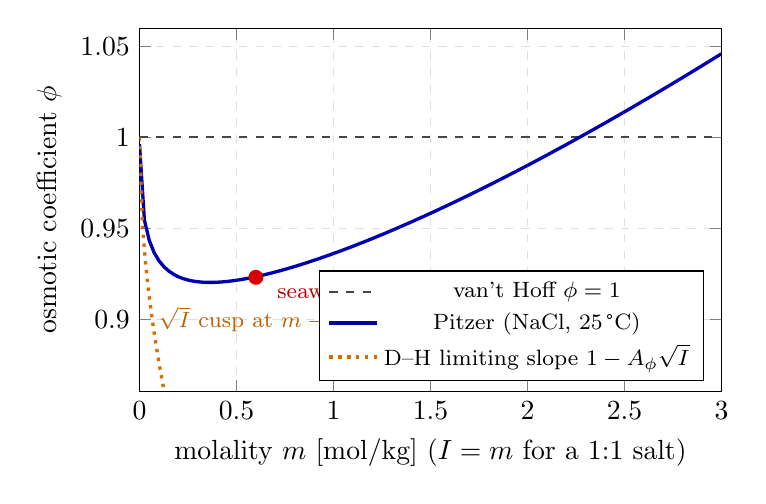
\begin{tikzpicture}
\begin{axis}[
    width=0.74\linewidth, height=6.2cm,
    xlabel={molality $m$ [mol/kg]  ($I=m$ for a 1:1 salt)},
    ylabel={osmotic coefficient $\phi$},
    xmin=0, xmax=3.0,
    ymin=0.86, ymax=1.06,
    grid=major,
    grid style={gray!25, dashed},
    legend pos=south east,
    legend style={font=\footnotesize},
]
\addplot[domain=0:3, samples=2, gray!55!black, thick, dashed]
   ({x},{1.0});
\addlegendentry{van't Hoff $\phi=1$}
\addplot[domain=0.0001:3, samples=120, blue!70!black, very thick]
   ({x},{1 - 0.391*sqrt(x)/(1+1.2*sqrt(x))
        + x*(0.0765+0.2664*exp(-2.0*sqrt(x)))
        + x*x*0.00127});
\addlegendentry{Pitzer (NaCl, 25\,\textdegree C)}
\addplot[domain=0:0.6, samples=40, orange!85!black, very thick, dotted]
   ({x},{1 - 0.391*sqrt(x)});
\addlegendentry{D--H limiting slope $1-A_\phi\sqrt I$}
\addplot[only marks, mark=*, mark size=2.5pt, mark options={red!85!black}]
   coordinates {(0.60, 0.923)};
\node[font=\footnotesize, text=red!70!black, anchor=west]
   at (axis cs:0.66,0.915) {seawater $\approx$0.6\,m};
\node[font=\footnotesize, text=orange!75!black, anchor=west]
   at (axis cs:0.05,0.90) {$\sqrt I$ cusp at $m\to0$};
\end{axis}
\end{tikzpicture}
\caption{Pitzer's osmotic coefficient for NaCl, the electrolyte analogue
of $\gamma$ correcting an ideal law.  The dashed grey line is the van't
Hoff ideal baseline $\phi=1$.  The dotted orange curve is the
Debye--H\"uckel limiting law $\phi\to 1-A_\phi\sqrt I$: note its infinite
slope (the $\sqrt I$ cusp) at infinite dilution---a singularity no
mole-fraction polynomial can reproduce.  The full Pitzer curve (blue)
follows this electrostatic dip, then the salt-specific pair term pulls it
back up, crossing $\phi=1$ near $m\approx 2.4$.  At seawater
concentration (red point, $\phi\approx0.92$) the real osmotic pressure is
about 8\,\% below van't Hoff---directly the back-pressure an RO membrane
need not overcome.}
\label{fig:pitzer-phi}
\end{figure}


Pitzer's ion-interaction model writes $\phi - 1$ as the sum of a
\emph{long-range} electrostatic term (a Debye--H\"uckel limiting law,
softened to stay finite) and \emph{short-range} ion-specific
corrections.  For a single 1:1 electrolyte it collapses to the compact
form Choupo implements:
\begin{equation}
   \boxed{\;
   \phi \;=\; 1
   \;\underbrace{-\,A_\phi\,\frac{\sqrt I}{1 + b\sqrt I}}_{\text{Debye--H\"uckel}}
   \;+\; m\,B^{\phi}
   \;+\; m^{2}\,C^{\phi},
   \;}
   \label{eq:pitzer-phi}
\end{equation}
with the second-virial coefficient itself a function of ionic
strength,
\begin{equation}
   B^{\phi} \;=\; \beta^{(0)} + \beta^{(1)}\,e^{-\alpha\sqrt I}.
   \label{eq:pitzer-B}
\end{equation}
Read term by term:

\begin{itemize}[leftmargin=*,nosep,topsep=2pt]
  \item \textbf{$-A_\phi\sqrt I/(1+b\sqrt I)$} --- the Debye--H\"uckel
        term.  $A_\phi \approx 0.391\,\mathrm{kg^{1/2}\,mol^{-1/2}}$ at
        25\,\textdegree C is the (universal, solvent-only) limiting-law
        slope; $b = 1.2$ is the universal closest-approach parameter.
        At low $I$ this $\sim -A_\phi\sqrt I$ behaviour is the exact
        electrostatic limit --- the famous square-root dependence that
        no mole-fraction polynomial can reproduce.  It \emph{lowers}
        $\phi$: ion screening reduces the effective particle count.
  \item \textbf{$m\,B^{\phi}$} --- the short-range, salt-specific pair
        interaction.  $\beta^{(0)}, \beta^{(1)}$ are tabulated per salt
        and \emph{raise} $\phi$ back up at higher $m$.  The
        exponential in \eqref{eq:pitzer-B} lets the pair term decay
        smoothly from its low-$I$ value $\beta^{(0)}+\beta^{(1)}$
        toward $\beta^{(0)}$; $\alpha = 2.0$ is the universal decay
        rate for 1:1 salts.
  \item \textbf{$m^{2}\,C^{\phi}$} --- a small triple-ion correction,
        important only in concentrated brine.
\end{itemize}

For NaCl at 25\,\textdegree C the simulator ships the standard set
\[
   \beta^{(0)} = 0.0765,\quad
   \beta^{(1)} = 0.2664,\quad
   C^{\phi} = 0.00127,\quad
   A_\phi = 0.391,\quad b = 1.2,\quad \alpha = 2.0,
\]
every one of which is a parameter the \code{osmotic} sub-block can
override (and a future \code{FitParameters} run could calibrate to a
measured $\phi(m)$ curve --- exactly the spirit of
Chapter~\ref{ch:lm}).

\begin{example}[NaCl at seawater concentration]
A 35\,g/L NaCl feed ($M = 58.44$\,g/mol) is $c \approx 0.60$\,kmol/m$^3$,
i.e.\ molality $m \approx 0.60$\,mol/kg, so $I = 0.60$ and
$\sqrt I = 0.775$.

\emph{Debye--H\"uckel term:}
\[
   -\,\frac{0.391 \times 0.775}{1 + 1.2 \times 0.775}
   \;=\; -\,\frac{0.303}{1.930}
   \;=\; -0.157.
\]
\emph{Pair term:}
$B^{\phi} = 0.0765 + 0.2664\,e^{-2.0 \times 0.775}
          = 0.0765 + 0.2664 \times 0.213 = 0.133$, so
$m B^{\phi} = 0.60 \times 0.133 = 0.080$.
\emph{Triple term:} $m^2 C^{\phi} = 0.36 \times 0.00127 = 0.0005$.

\[
   \phi \;=\; 1 - 0.157 + 0.080 + 0.0005 \;\approx\; 0.923.
\]
The osmotic pressure is therefore about \textbf{7.7\,\% lower} than
van't Hoff predicts:
\[
   \pi_{\text{vH}} = \nu \Rgas T c
   = 2 \times 8.314 \times 298 \times 599 \approx 29.7~\text{bar},
   \qquad
   \pi_{\text{Pitzer}} \approx 0.923 \times 29.7 \approx 27.4~\text{bar}.
\]
Against a 55\,bar applied pressure that $\sim$2.3\,bar relief in the
back-pressure is not cosmetic: it raises the net driving pressure
$\Delta P - \Delta\pi$ and therefore the water flux and the recovery.
\end{example}

\subsection{Why this matters for NF/RO --- and where it is worst}

The osmotic correction looks modest at the feed (8\,\% here), but the
quantity that actually throttles the flux is the osmotic pressure
\emph{at the membrane wall}, not in the bulk.  Concentration
polarisation (Chapter~\ref{ch:why-transport} and the membrane
tutorials) piles solute up against the wall, $c_m = c_b\,e^{J_w/k}$,
so the wall concentration can be several times the feed.  The
correction $(1-\phi)\,\nu\Rgas T c$ therefore reaches its largest
magnitude --- and, at brine concentrations, can even change sign ---
exactly at the wall, where the membrane is most starved; getting $\phi$
right matters most there.  This is the bread-and-butter regime of
Vítor's NF/RO research, and the reason the Pitzer model is the first
electrolyte refinement Choupo carries.

\begin{keyidea}
The osmotic pressure is built in two independent layers, mirroring the
whole simulator's ``ideal baseline $+$ correction'' design.  The
\emph{exact} thermodynamics is $\pi = -(\Rgas T/\bar V_w)\ln a_w$; the
\emph{model} supplies $\ln a_w$ through one dimensionless number
$\phi$.  van't Hoff sets $\phi = 1$ (ideal); Pitzer makes $\phi$ a
function of ionic strength, capturing the $\sqrt I$ electrostatic
limit that no polynomial activity model can.  The two are
interchangeable \code{OsmoticModel} sub-models --- a one-word change
in the case.
\end{keyidea}

\begin{tutoriallink}
\file{tutorials/steady/membranes/membrane06\_pitzer} --- the seawater RO case of
\file{membrane01} with \code{osmotic \{ model Pitzer; \}}; $\phi
\approx 0.92$ lifts recovery from 15.6\,\% to 17.2\,\%.
\file{tutorials/steady/membranes/membrane01\_RO\_NaCl\_seawater} is the van't
Hoff baseline for comparison; \file{membrane03} sweeps $k_{\text{film}}$
to expose the concentration-polarisation curve where the osmotic model
matters most.
\end{tutoriallink}

% ---------------------------------------------------------------------
\section{Electrolyte-NRTL: the activity coefficient of the
\emph{ion}}\label{ch:enrtl}

\begin{whatyoulllearn}
Pitzer's $\phi(I)$ (\S\ref{ch:electrolytes}) gives the deviation of the
\emph{solvent} --- the osmotic pressure that throttles an RO membrane.
But an evaporator, a crystalliser, or a drowning-out precipitator needs
the deviation of the \emph{salt}: the mean ionic activity coefficient
$\gamma_\pm$, which fixes the boiling-point rise and the supersaturation
ratio.  This chapter derives the \emph{electrolyte-NRTL} (eNRTL) model
of Chen, Song and Evans~\cite{ChenSongEvans1982,ChenEvans1986}, the
natural extension of the molecular NRTL of \S\ref{ch:activity} to a
solution of ions.  Its premise is a clean
\emph{three-layer} split of the excess Gibbs energy --- a long-range
Pitzer--Debye--H\"uckel (PDH) term for the ion atmosphere, a short-range
local-composition (NRTL) term for the molecular neighbourhood, and (for
a mixed solvent) a Born term for transferring an ion between dielectrics
--- each one a separately readable contribution to $\ln\gamma_\pm$.  We
write the closed form Choupo evaluates for one fully-dissociated 1:1
salt, give the $T$-dependence, and validate it against Hamer \& Wu NaCl
data to AAD~1.8\,\%.
\end{whatyoulllearn}

\subsection{Why a second electrolyte model?}

The Pitzer osmotic model of \S\ref{ch:electrolytes} answers exactly one
question --- \emph{what is the water activity $a_w$?} --- and answers it
beautifully (NaCl $\phi$ to $<0.2$\,\%).  That is all an RO designer
needs, because the flux is set by $\Delta\pi \propto -\ln a_w$.  But
move to a process that \emph{concentrates} or \emph{precipitates} the
salt and the governing quantity flips to the salt's own activity:

\begin{itemize}[leftmargin=*,nosep,topsep=2pt]
  \item an \textbf{evaporator} raises the boiling point by
        $\propto -\ln a_w$, but the duty and the achievable
        concentration are bounded by where the salt \emph{saturates},
        i.e.\ by $\gamma_\pm$;
  \item a \textbf{crystalliser} nucleates when the activity product
        $(\gamma_\pm m)^{\nu}$ exceeds $K_{sp}$ --- the driving force is
        $\gamma_\pm$, not $m$;
  \item a \textbf{drowning-out} (antisolvent) precipitator works
        \emph{because} adding ethanol drops the dielectric constant,
        which \emph{raises} $\gamma_\pm$ and so the supersaturation ---
        an effect with no counterpart in a single-solvent model.
\end{itemize}

eNRTL supplies $\gamma_\pm$ \emph{and} $a_w$ from one consistent
excess-Gibbs surface, and --- unlike Pitzer, whose virial coefficients
are tied to molality in pure water --- it lives on the mole-fraction
scale, so it extends naturally to the mixed solvent.  In Choupo it is
the \code{activity \{ model eNRTL; \}} sub-model of the same electrolyte
slot that carries Pitzer
(\code{src/thermo/electrolyte/ENRTLSingleSalt.H}).

\subsection{The three-layer excess Gibbs energy}

\begin{figure}[ht]
\centering
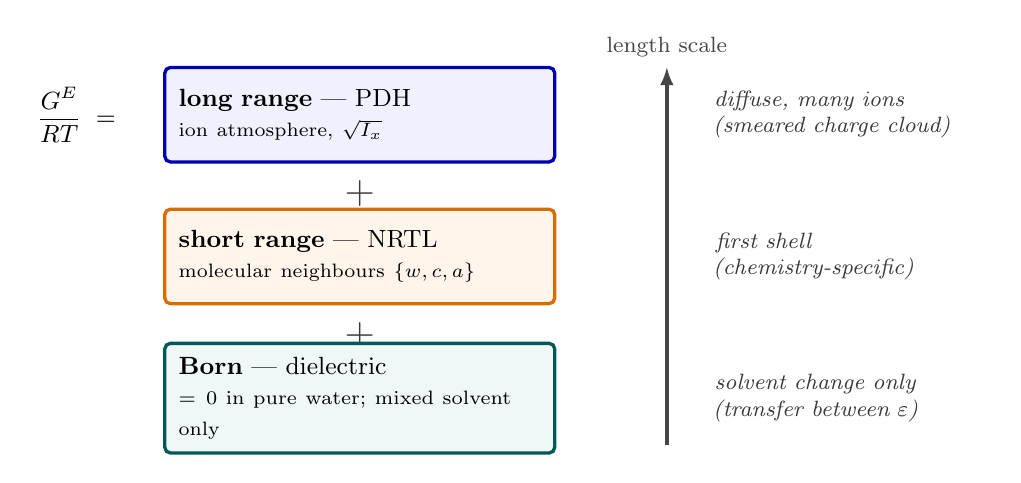
\begin{tikzpicture}[
    layer/.style={draw, very thick, rounded corners=2pt, align=left,
                  font=\small, inner sep=5pt, minimum height=12mm,
                  text width=46mm},
    pdh/.style={layer, draw=blue!70!black, fill=blue!6},
    lc/.style={layer, draw=orange!85!black, fill=orange!8},
    born/.style={layer, draw=teal!70!black, fill=teal!6},
    plus/.style={font=\Large, text=gray!45!black},
    note/.style={font=\footnotesize\itshape, text=gray!45!black,
                 align=left, text width=34mm},
]
\node[font=\small] (tot) at (0,4.4)
   {$\dfrac{G^{E}}{RT}\;=$};
\node[pdh]  (a) at (3.6,4.4) {\textbf{long range} --- PDH\\ \scriptsize ion atmosphere, $\sqrt{I_x}$};
\node[plus] at (3.6,3.4) {$+$};
\node[lc]   (b) at (3.6,2.6) {\textbf{short range} --- NRTL\\ \scriptsize molecular neighbours $\{w,c,a\}$};
\node[plus] at (3.6,1.6) {$+$};
\node[born] (c) at (3.6,0.8) {\textbf{Born} --- dielectric\\ \scriptsize $=0$ in pure water; mixed solvent only};
\draw[->, >=latex, very thick, gray!55!black] (7.5,0.2) -- (7.5,5.0)
   node[anchor=south, font=\footnotesize]{length scale};
\node[note, anchor=west] at (8.0,4.4) {diffuse, many ions\\ (smeared charge cloud)};
\node[note, anchor=west] at (8.0,2.6) {first shell\\ (chemistry-specific)};
\node[note, anchor=west] at (8.0,0.8) {solvent change only\\ (transfer between $\varepsilon$)};
\end{tikzpicture}
\caption{Electrolyte-NRTL splits the excess Gibbs energy into three
separately-readable layers, each acting on a different length scale---the
model's whole idea.  The \emph{long-range} Pitzer--Debye--H\"uckel term
(blue) sees only the diffuse ion atmosphere and its $\sqrt{I_x}$
electrostatics; the \emph{short-range} local-composition NRTL term
(orange) sees an ion's immediate molecular neighbours
$\{w,c,a\}$ and carries the chemistry-specific interactions; the Born term
(teal) enters only when the solvent's dielectric constant changes, and is
identically zero in pure water.  Because they act on different scales they
simply \emph{add}, and $\ln\gamma_\pm$ for each species is the
corresponding derivative---an evaporator and a crystalliser read the same
surface that an RO membrane does.}
\label{fig:enrtl-layers}
\end{figure}


eNRTL writes the molar excess Gibbs energy as a sum of physically
distinct contributions,
\begin{equation}
   \frac{G^{E}}{RT}
   \;=\;
   \underbrace{\frac{G^{E,\mathrm{PDH}}}{RT}}_{\text{long range}}
   \;+\;
   \underbrace{\frac{G^{E,\mathrm{lc}}}{RT}}_{\text{short range (NRTL)}}
   \;+\;
   \underbrace{\frac{G^{E,\mathrm{Born}}}{RT}}_{\text{dielectric transfer}},
   \label{eq:enrtl-gibbs}
\end{equation}
and the activity coefficient of every species is the corresponding
derivative.  The split is the model's whole idea: an ion feels the
diffuse \emph{ion atmosphere} (a smeared-out, charge-only effect that
only the PDH term knows about) \emph{and} its immediate \emph{molecular
neighbours} (a short-range, chemistry-specific effect that only the
local-composition term knows about).  The two act on different length
scales, so they add.  The Born term enters only when the solvent itself
changes (the mixed-solvent case, \S\ref{sec:enrtl-mixed}); in pure water
it is identically zero.

\paragraph{Reference state --- unsymmetric for ions.}
A neutral component's $\gamma\!\to\!1$ as $x\!\to\!1$ (the pure liquid,
\S\ref{ch:activity}).  An ion has no pure liquid, so its reference is
the \emph{unsymmetric} (aqueous infinite-dilution) convention:
$\gamma_i^{*}\!\to\!1$ as the salt $\to 0$ in pure water.  In the code
this is enforced literally --- every ionic local term is evaluated at
the actual composition \emph{minus} its value at $\mathbf{X}_{\text{ref}} =
(x_w{=}1,\,x_c{=}0,\,x_a{=}0)$ --- so the subtraction $lc(\mathbf X) -
lc(\mathbf X_{\text{ref}})$ in \code{ENRTLSingleSalt.H} \emph{is} the
unsymmetric normalisation.  The solvent (water) keeps the ordinary
symmetric reference ($\gamma_w\!\to\!1$ as $x_w\!\to\!1$).

\subsection{Long range: the Pitzer--Debye--H\"uckel term}

For the long-range part eNRTL borrows Pitzer's mole-fraction-scale
Debye--H\"uckel expression.  Its contribution to the \emph{unsymmetric}
ionic $\ln\gamma$ is
\begin{equation}
   \ln\gamma_i^{\mathrm{PDH}}
   \;=\;
   -A_{\mathrm{DH}}
   \left[
      \frac{2 z_i^{2}}{\rho}\,\ln\!\bigl(1 + \rho\sqrt{I_x}\bigr)
      \;+\;
      \frac{z_i^{2}\sqrt{I_x} - 2\,I_x^{3/2}}{1 + \rho\sqrt{I_x}}
   \right],
   \label{eq:enrtl-pdh}
\end{equation}
where $I_x = \tfrac12\sum_i x_i z_i^{2}$ is the \emph{mole-fraction}
ionic strength (note: $x_i$, not molality $m_i$ --- eNRTL lives on the
mole-fraction scale), $\rho = 14.9$ is the closest-approach parameter
(Pitzer's universal value), and $A_{\mathrm{DH}}$ is the
mole-fraction-scale Debye--H\"uckel slope,
\begin{equation}
   A_{\mathrm{DH}}
   \;=\;
   \frac13
   \sqrt{\frac{2\pi N_{\!A}}{\bar V_w}}
   \left(\frac{e^{2}}{4\pi\varepsilon_w\varepsilon_0 k_B T}\right)^{\!3/2},
   \label{eq:enrtl-ADH}
\end{equation}
which evaluates to $A_{\mathrm{DH}} = 2.9127$ for water at 25\,\textdegree C
($\bar V_w = 1.807\times10^{-5}$\,m$^3$/mol, $\varepsilon_w = 78.45$).
The solvent term gets the symmetric companion
$\ln\gamma_w^{\mathrm{PDH}} = 2 A_{\mathrm{DH}}\,I_x^{3/2}/(1+\rho\sqrt{I_x})$.
This is the same $\sqrt I$ electrostatic limit as Pitzer's
\eqref{eq:pitzer-phi} --- the part no polynomial activity model can
reproduce --- just written for $\ln\gamma$ instead of $\phi$ and on the
mole-fraction basis.

\subsection{Short range: the local-composition (NRTL) term}

The short-range term is the NRTL local-composition idea of
\S\ref{ch:activity}, now applied to a mixture of \emph{three} species
$\{w, c, a\}$ (water, cation, anion) with two rules borrowed from
Chen's electrolyte theory:

\begin{itemize}[leftmargin=*,nosep,topsep=2pt]
  \item \textbf{like-ion repulsion}: no cation sits next to a cation
        (Coulomb forbids it), so a like-charged species is \emph{excluded}
        from an ion's local cell;
  \item \textbf{local electroneutrality}: the immediate neighbourhood of
        a central molecule is charge-balanced.
\end{itemize}

With a single salt the energy landscape collapses to just \emph{two}
adjustable numbers --- the molecule\,$\to$\,electrolyte and
electrolyte\,$\to$\,molecule interaction energies $\tau_{m,ca}$ and
$\tau_{ca,m}$ --- plus the nonrandomness factor $\alpha$.  The Boltzmann
factors are the familiar NRTL form $G_{ij} = \exp(-\alpha\,\tau_{ij})$,
and all ion--ion same-pair terms vanish ($\tau_{ca}=0$, $G_{ca}=1$).
The resulting ionic local-composition $\ln\gamma$ is the
Chen--Song--Evans three-term expression (as implemented in
\code{ENRTLSingleSalt::lnGammaX}, following IDAES Eqns.~26--27),
\begin{equation}
   \ln\gamma_s^{\mathrm{lc}}
   \;=\;
   z_s\!\left[
      \frac{X_w G_{sw}}{\sum_k X_k G_{kw}}
      \!\left(\tau_{sw} - \frac{\sum_k X_k G_{kw}\tau_{kw}}{\sum_k X_k G_{kw}}\right)
      +\frac{\sum_{k}^{\prime} X_k G_{ks}\tau_{ks}}{\sum_{k}^{\prime} X_k G_{ks}}
      +\frac{X_{s'} G_{s s'}}{\sum_k^{\prime\prime} X_k G_{k s'}}
       \!\left(\tau_{s s'} - \frac{\sum_k^{\prime\prime} X_k G_{k s'}\tau_{k s'}}{\sum_k^{\prime\prime} X_k G_{k s'}}\right)
   \right],
   \label{eq:enrtl-lc}
\end{equation}
where $s'$ is the ion of \emph{opposite} charge to $s$; the primed sums
$\sum'$ exclude the species like-charged with $s$, and the
double-primed sums $\sum''$ exclude the species like-charged with $s'$
(the repulsion rule).  Read it as the three neighbourhoods an ion sees:
term~1 the solvent cell, term~2 its own charge cell, term~3 the
counter-ion cell.  The mean ionic value follows from the salt's
stoichiometry,
\begin{equation}
   \ln\gamma_\pm^{(x)}
   \;=\;
   \frac{\nu_c\bigl(\ln\gamma_c^{\mathrm{PDH}}+\ln\gamma_c^{\mathrm{lc}}\bigr)
        +\nu_a\bigl(\ln\gamma_a^{\mathrm{PDH}}+\ln\gamma_a^{\mathrm{lc}}\bigr)}
        {\nu_c+\nu_a},
   \qquad
   \gamma_\pm = \gamma_\pm^{(x)}\Big/\!\bigl(1 + 10^{-3}M_w\,\nu\,m\bigr),
   \label{eq:enrtl-mean}
\end{equation}
the divisor converting the mole-fraction-scale $\gamma_\pm^{(x)}$ to the
molality-scale $\gamma_\pm$ that lab data report ($M_w$ the solvent
molar mass in g/mol, $\nu = \nu_c+\nu_a$).

\subsection{Temperature dependence}

Three places in the model carry $T$, and Choupo handles each by anchoring
to the validated 25\,\textdegree C kernel so that every existing golden
master stays byte-identical at the reference and moves physically away
from it:

\begin{enumerate}[leftmargin=*,nosep,topsep=2pt]
  \item \textbf{NRTL energies.}  Like the molecular NRTL's
        $\tau = a + b/T$, the electrolyte $\tau$ is taken in the
        $\Delta g/RT$ form with a $T$-independent interaction energy,
        \begin{equation}
           \tau_{ij}(T) = \tau_{ij}^{\mathrm{ref}}\,\frac{T_{\mathrm{ref}}}{T},
           \qquad T_{\mathrm{ref}} = 298.15\,\mathrm K,
        \end{equation}
        i.e.\ $a=0$, $b = \tau^{\mathrm{ref}} T_{\mathrm{ref}}$ --- the
        single published 25\,\textdegree C value sets $b$ and the form
        reduces to $\tau^{\mathrm{ref}}$ at the reference.
  \item \textbf{Debye--H\"uckel slope.}  $A_{\mathrm{DH}}(T) =
        A_{\mathrm{DH}}(25)\,f(T)$ with the Born--Bjerrum factor
        \begin{equation}
           f(T) = \Bigl(\frac{\rho_w(T)}{\rho_w(25)}\Bigr)^{1/2}
                  \Bigl(\frac{\varepsilon_w(25)\,T_{25}}{\varepsilon_w(T)\,T}\Bigr)^{3/2},
        \end{equation}
        evaluated through the Malmberg--Maryott $\varepsilon_w(T)$ and
        Kell $\rho_w(T)$ correlations
        (\code{src/thermo/electrolyte/SolventProperties.H}); $f(25)=1$.
  \item \textbf{Born and PDH} are evaluated at the actual $T$, never a
        hard-coded 298.15.
\end{enumerate}

\begin{pitfall}
The anchored $\tau(T) \propto 1/T$ is a \emph{calorimetrically
uncalibrated} guess: it reproduces $\gamma_\pm$ and $\phi$ at and near
25\,\textdegree C, but its temperature \emph{slope} (hence any heat of
dilution derived from it) has not been refitted against
$\mathrm{d}H$ data.  This is the same caveat that gates the Pitzer
$L_\phi$ enthalpy branch; the eNRTL package deliberately does \emph{not}
inherit the \code{calorimetricFit} flag, so it stays in the honest,
uncalibrated regime.  Use it for $\gamma_\pm$, $a_w$, boiling-point rise
and solubility; do not read a heat of dilution off its $T$-slope without
a refit.
\end{pitfall}

\subsection{The mixed solvent: drowning-out and the Born
term}\label{sec:enrtl-mixed}

Add an antisolvent (ethanol) at salt-free mole fraction $x_{\mathrm{anti}}$
and two things happen, both of which eNRTL captures from
\eqref{eq:enrtl-gibbs}:

\begin{enumerate}[leftmargin=*,nosep,topsep=2pt]
  \item \textbf{Dielectric mixing.}  The mixture permittivity
        $\varepsilon_{\mathrm{mix}}$ (a mass-fraction average of the two
        pure values), molar volume $\bar V_{\mathrm{mix}}$ and molar mass
        $M_{\mathrm{mix}}$ replace the pure-water values in
        \eqref{eq:enrtl-ADH}.  Because $\varepsilon_{\mathrm{mix}} <
        \varepsilon_w$, the slope $A_{\mathrm{DH}}$ \emph{grows} (electrostatics
        is less screened in a less polar medium) --- the PDH term
        strengthens.
  \item \textbf{Born transfer.}  Moving an ion from pure water
        ($\varepsilon_w$) into the lower-$\varepsilon$ mixture costs the
        Born self-energy difference,
        \begin{equation}
           \ln\gamma_i^{\mathrm{Born}}
           \;=\;
           \frac{e^{2}}{8\pi\varepsilon_0 k_B T}
           \left(\frac{1}{\varepsilon_{\mathrm{mix}}}
                - \frac{1}{\varepsilon_w}\right)\frac{1}{r_i},
           \label{eq:enrtl-born}
        \end{equation}
        with $r_i$ the Born radius (calibrated to KCl in water+ethanol).
        It is positive --- the ion is \emph{less} comfortable in the
        mixture --- so $\gamma_\pm$ rises.
\end{enumerate}

Both effects push $\gamma_\pm$ up, which lifts the activity product
$(\gamma_\pm m)^\nu$ above $K_{sp}$ and \emph{precipitates} the salt
without removing any water --- the thermodynamic engine of antisolvent
crystallisation.  In Choupo this is the \code{gammaPMMixed} entry point;
$x_{\mathrm{anti}}\!\to\!0$ recovers the aqueous $\gamma_\pm$ exactly,
and $T\!=\!298.15$ recovers the validated 25\,\textdegree C kernel.

\begin{example}[NaCl mean ionic activity coefficient at 25\,\textdegree C]
Take $m = 1.0$\,mol/kg NaCl ($\nu_c=\nu_a=1$, $z_c=z_a=1$, $M_w=18.015$).
The solvent amount is $n_w = 1000/18.015 = 55.51$\,mol/kg, so
$n_{\text{tot}} = 55.51 + 2(1.0) = 57.51$ and the mole fractions are
$X_w = 0.9652$, $X_c = X_a = 0.01739$, giving a mole-fraction ionic
strength $I_x = \tfrac12(0.01739 + 0.01739) = 0.01739$, $\sqrt{I_x} =
0.1319$.

\emph{PDH term} (Eq.~\ref{eq:enrtl-pdh}, $z=1$, $A_{\mathrm{DH}}=2.9127$,
$\rho=14.9$):
\[
   \ln\gamma_c^{\mathrm{PDH}}
   = -2.9127\!\left[\frac{2}{14.9}\ln(1+14.9\times0.1319)
   + \frac{0.1319 - 2(0.01739)^{3/2}}{1+14.9\times0.1319}\right]
   \approx -0.252.
\]
\emph{Local term} (Eq.~\ref{eq:enrtl-lc}, with $\tau_{m,ca}=8.885$,
$\tau_{ca,m}=-4.549$, $\alpha=0.2$, evaluated unsymmetrically) adds a
positive short-range contribution; summed and mole-fraction-to-molality
converted via \eqref{eq:enrtl-mean} the kernel returns
\[
   \gamma_\pm \;\approx\; 0.648,
\]
against the Hamer \& Wu tabulated value $0.657$ --- a $1.3$\,\% error,
typical of the model across the range.
\end{example}

\subsection{Validation and the power-and-limit}

The kernel was checked term-by-term against an independent Python
prototype (\file{bin/curate/enrtl\_ref/enrtl\_validated.py}, agreeing to
$5\times10^{-5}$) and against the classic NaCl reference data of
Hamer \& Wu~\cite{HamerWu1972} (and Robinson \& Stokes) over
$0.1$--$6$\,mol/kg at 25\,\textdegree C:

\begin{center}
\begin{tabular}{r r r r}
\hline
$m$ (mol/kg) & eNRTL $\gamma_\pm$ & lit.\ $\gamma_\pm$ & error \\
\hline
0.1 & 0.773 & 0.778 & $-0.6$\,\% \\
0.5 & 0.670 & 0.681 & $-1.7$\,\% \\
1.0 & 0.648 & 0.657 & $-1.3$\,\% \\
2.0 & 0.674 & 0.668 & $+0.9$\,\% \\
3.0 & 0.732 & 0.714 & $+2.5$\,\% \\
6.0 & 0.950 & 0.986 & $-3.6$\,\% \\
\hline
\multicolumn{4}{l}{AAD $\gamma_\pm = 1.8$\,\%;\quad osmotic $\phi$ AAD $= 1.4$\,\%}\\
\hline
\end{tabular}
\end{center}

The eNRTL captures the entire shape: the dip near $m\approx 1$ (PDH
screening dominates) and the strong rise past $m\approx 3$ (the local
term takes over) --- the same non-monotone curve van't Hoff cannot see.

\begin{keyidea}
\textbf{Power.}  One mole-fraction-scale excess-Gibbs surface delivers
both $\gamma_\pm$ \emph{and} $a_w$ from two energy parameters per salt,
extends without re-parameterisation to mixed solvents (the Born term is
parameter-light), and reproduces the non-monotone $\gamma_\pm(m)$ to
$\sim$2\,\% --- the engine behind boiling-point rise, solubility, and
antisolvent crystallisation.

\textbf{Limit.}  Choupo's kernel is a \emph{single fully-dissociated
salt}; it does not by itself do multi-salt common-ion mixtures, ion
pairing, or weak-electrolyte speciation (those live on the multi-ion
Pitzer speciation path of
\S\ref{ch:pitzer-hmw}).  Its $T$-slope is calorimetrically uncalibrated
(\code{calorimetricFit} stays off), and for high-concentration
\emph{aqueous} accuracy a per-salt-fitted Pitzer ($\sim$0.2\,\%) beats
it ($\sim$1.8\,\%) --- eNRTL's edge is the mixed solvent and the unified
$\gamma_\pm$/$a_w$ surface, not single-salt aqueous precision.
\end{keyidea}

\begin{tutoriallink}
\file{tutorials/steady/evaporation/evaporator07\_nacl\_enrtl} --- a NaCl
evaporator with \code{activity \{ model eNRTL; \}}, where $\gamma_\pm$
sets the boiling-point rise and the saturation limit.
\file{tutorials/steady/crystallisation/crystalliser06\_nacl\_antisolvent}
exercises the mixed-solvent Born term (ethanol drowning-out).  Contrast
with the Pitzer membrane cases of \S\ref{ch:electrolytes}
(\file{membrane06\_pitzer}), which solve the \emph{solvent} side of the
same physics.
\end{tutoriallink}

\subsection{Multi-salt eNRTL: the symmetric multicomponent
formulation}\label{sec:enrtl-multisalt}

When two salts share the water --- NaCl $+$ KCl in a crystalliser purge, a
mixed brine --- each ion's environment contains \emph{foreign} ions, and the
single-salt expressions no longer apply.  The multicomponent formulation
(Song \& Chen 2009, DOI \texttt{10.1021/ie9004578})
keeps the two eNRTL hypotheses (local electroneutrality, like-ion repulsion)
and writes the local term species-wise, with every effective ion--molecule
and ion--ion binary assembled from the \emph{pair} parameters by
charge-fraction mixing rules:
\begin{equation}
  Y_c = \frac{X_c}{\sum_{c'} X_{c'}}, \qquad
  G_{am} = \sum_{c} Y_c\, G_{ca,m}, \qquad
  G_{ca} = \sum_{c'} Y_{c'}\, G_{ca,c'a}, \qquad
  \tau = -\ln G / \alpha,
\end{equation}
so a chloride ion in a Na/K mixture sees a \emph{composition-weighted}
water--salt energy.  The long-range term is the same PDH expression with the
multicomponent ionic strength.  Two structural results, both golden-locked in
the tutorial:

\begin{enumerate}[leftmargin=*,nosep,topsep=2pt]
  \item \textbf{Exact single-salt reduction.}  With one salt the charge
        fractions collapse to unity and the model IS the single-salt kernel
        of the previous sections (the tutorial pins the pure endpoints at
        $\sim 10^{-15}$ relative).
  \item \textbf{Harned's rule emerges.}  At constant total molality,
        $\ln\gamma_\pm$ of each salt is nearly \emph{linear} in the salt
        fraction ($R^2 > 0.999$ at 4\,mol/kg with zero
        electrolyte--electrolyte parameters) --- the century-old empirical
        rule falls out of the local-composition structure.
\end{enumerate}

\begin{intuition}
\textbf{A declared inconsistency --- and its fix, side by side.}  The published
multicomponent activity-coefficient expressions differentiate the excess
Gibbs energy \emph{treating the mixing-rule binaries as constants}, yet those
binaries depend on composition through the charge fractions $Y$.  The result
is not exactly Gibbs--Duhem consistent --- the motivation for the
\emph{refined} eNRTL of Bollas, Chen \& Barton (2008).  Choupo ships
\textbf{both formulations} (\code{formulation published;} vs
\code{consistent;}): the consistent one keeps the chain rule through the
$Y$-dependent mixing rules, so $\gamma$ \emph{is} the exact derivative of
$G^{ex}$ and the finite-difference oracle closes ($\sim$$10^{-9}$) at
\emph{every} composition --- while the published one prints its mid-sweep
deviation ($\sim$$0.5$) next to the pure-salt state where it, too, is exact.
At 4\,mol/kg NaCl--KCl the two differ by $\sim$4\,\% in mid-sweep
$\gamma_\pm$.  Robinson's 1961 isopiestic data judge them: the published form
wins the dominant Harned coefficient ($\alpha_{\mathrm{NaCl}}$ +14\,\% vs
$-29\,\%$), both overstate the small $\alpha_{\mathrm{KCl}}$, and no single
$\tau_{EE}$ closes both --- the residual is structural.  Bollas et al.'s own
Figure~1 (this very system) cross-checks both branches: their original-eNRTL
panel matches our published curves to the pixel, and their refined panel
shows the same signature our consistent form shows --- the $\tau$ fan nearly
collapses, because an exact derivative is almost insensitive to
$\tau_{EE}$.
\end{intuition}

\begin{tutoriallink}
\file{tutorials/props/electrolyte/enrtl\_multisalt\_nacl\_kcl} --- the
paper's own demonstration (NaCl--KCl--H$_2$O, 4\,mol/kg Harned sweep),
reproducing its Figure~1 $\tau_{ca,c'a}$ sensitivity fan (in log$_{10}$ ---
the figure's axis label says $\ln$ but plots log$_{10}$) and locking the
reduction pin, the Harned slopes, and the declared Gibbs--Duhem deviation.
\end{tutoriallink}

% =====================================================================
\section{Multi-ion Pitzer: the Harvie--M\o ller--Weare
model}\label{ch:pitzer-hmw}

\begin{whatyoulllearn}
The single-salt osmotic coefficient of the previous section answers ``how
much does \emph{this one} dissolved salt lower the water activity?'' Real
brines, seawater, scaling waters and the inside of an evaporator carry
\emph{many} ions at once --- $\text{Na}^+$, $\text{K}^+$, $\text{Ca}^{2+}$,
$\text{Mg}^{2+}$, $\text{Cl}^-$, $\text{SO}_4^{2-}$, $\text{OH}^-$, the
carbonates --- and an ion's activity then depends on \emph{every} ion
present, not just its own counter-ion.  This section builds the
Harvie--M\o ller--Weare (HMW) assembly of Pitzer's model, which gives a
\emph{per-ion} activity coefficient $\gamma_i$ from the same long-range
Debye--H\"uckel term plus binary virials \emph{plus} ternary mixing terms.
We show exactly the sums Choupo evaluates (\code{PitzerHMW::evaluate}),
the higher-order electrostatic term $E_\theta(I)$ that no other Pitzer
code makes optional, and the self-test that proves the multi-ion model
collapses to the single-salt kernel of \S\ref{ch:electrolytes}.
\end{whatyoulllearn}

\subsection{From one salt to many ions}

The compact form \eqref{eq:pitzer-phi} is what you get when the general
Pitzer expansion is specialised to a \emph{single} fully dissociated
salt.  The general expansion does not work with salts at all --- it works
with \emph{ions}.  Its natural output is not a mean activity
coefficient $\gamma_\pm$ but an individual $\gamma_i$ for each ionic
species $i$, on the molality scale, referenced to infinite dilution in
pure water.  Two reasons force this move:

\begin{itemize}[leftmargin=*,nosep,topsep=2pt]
  \item \textbf{A speciation solver needs $\gamma_i$, not $\gamma_\pm$.}
        When the same water carries dissolved $\text{CO}_2$ that
        speciates into $\text{HCO}_3^-$ and $\text{CO}_3^{2-}$, or when
        you solve for pH, the chemical-equilibrium solver
        (\code{SpeciationSolver}) writes a mass-action law for each
        reaction and needs the activity of \emph{each} ion individually.
        A lumped $\gamma_\pm$ cannot be unbundled.
  \item \textbf{Cross interactions are real.}  In a mixed
        $\text{Na}^+/\text{Mg}^{2+}/\text{Cl}^-/\text{SO}_4^{2-}$ brine
        the activity of $\text{Na}^+$ is changed by the presence of
        $\text{Mg}^{2+}$ (a like-sign neighbour) and of $\text{SO}_4^{2-}$
        (a second anion it never pairs with as a pure salt).  These are
        the \emph{mixing terms}; they are zero in any single-salt
        solution and are precisely what HMW adds.
\end{itemize}

Choupo implements the HMW assembly as the \code{pitzer} \code{AqueousActivity}
model (\code{PitzerHMW}), selected by the same one word a single-salt
case uses --- \code{activityModel pitzer;} --- but now reached through the
speciation path, where it replaces the cheap Davies fallback with a full
per-ion $\gamma_i$.  All the arithmetic comes from the \emph{same}
\code{PitzerForm} header the single-salt kernel uses, so there is one
Pitzer surface in the code, never two that can drift apart.

\subsection{The per-ion working equations}

For a cation $M$ (charge $z_M$) and an anion $X$ (charge $z_X$, here
$z_X<0$), in a solution of cations $\{c\}$, anions $\{a\}$ and neutrals
$\{n\}$ at molalities $m_i$, ionic strength
$I=\tfrac12\sum_i z_i^2 m_i$, the HMW equations Choupo evaluates are
(Pitzer 1991, ch.~3; \cite{HMW1984})

\begin{equation}
\begin{aligned}
   \ln\gamma_M \;=\;& z_M^2\,F
     \;+\; \sum_a m_a\bigl(2B_{Ma} + Z\,C_{Ma}\bigr)
     \;+\; |z_M|\sum_c\sum_a m_c m_a\,C_{ca} \\[2pt]
   &+\; \sum_{c} m_c\Bigl(2\Phi_{Mc} + \sum_a m_a\,\psi_{Mca}\Bigr)
     \;+\; \sum_{a<a'} m_a m_{a'}\,\psi_{Maa'},
\end{aligned}
   \label{eq:hmw-cation}
\end{equation}
\begin{equation}
\begin{aligned}
   \ln\gamma_X \;=\;& z_X^2\,F
     \;+\; \sum_c m_c\bigl(2B_{cX} + Z\,C_{cX}\bigr)
     \;+\; |z_X|\sum_c\sum_a m_c m_a\,C_{ca} \\[2pt]
   &+\; \sum_{a} m_a\Bigl(2\Phi_{Xa} + \sum_c m_c\,\psi_{Xac}\Bigr)
     \;+\; \sum_{c<c'} m_c m_{c'}\,\psi_{Xcc'},
\end{aligned}
   \label{eq:hmw-anion}
\end{equation}
with the long-range function $F$ collecting the Debye--H\"uckel slope and
the ionic-strength \emph{derivatives} of the binary and mixing terms,
\begin{equation}
   F \;=\;
   \underbrace{-A_\phi\!\left[\frac{\sqrt I}{1+b\sqrt I}
     + \frac{2}{b}\ln\!\bigl(1+b\sqrt I\bigr)\right]}_{\text{Debye--H\"uckel}}
   \;+\; \sum_c\sum_a m_c m_a\,B'_{ca}
   \;+\; \sum_{c<c'} m_c m_{c'}\Phi'_{cc'}
   \;+\; \sum_{a<a'} m_a m_{a'}\Phi'_{aa'},
   \label{eq:hmw-F}
\end{equation}
and the charge-weighted total molality
\begin{equation}
   Z \;=\; \sum_i |z_i|\,m_i .
   \label{eq:hmw-Z}
\end{equation}

Reading these against the code (\code{PitzerHMW::evaluate}), every symbol
is one of a handful of \code{PitzerForm} calls:

\begin{itemize}[leftmargin=*,nosep,topsep=2pt]
  \item $B_{ca}=\beta^{(0)}_{ca}+\beta^{(1)}_{ca}\,g(\alpha_1\sqrt I)
        +\beta^{(2)}_{ca}\,g(\alpha_2\sqrt I)$, with
        $g(x)=2\bigl[1-(1+x)e^{-x}\bigr]/x^2$ --- the binary pair term,
        per (cation, anion) read from the shared catalogue
        \file{data/standards/electrolyte/pairs.dat}.  The $\beta^{(2)}$
        slot is the 2:2 ion-pairing term ($\alpha_1=1.4$, $\alpha_2=12$);
        it is zero for 1:1/2:1/1:2 salts.
  \item $B'_{ca}=\bigl[\beta^{(1)}_{ca}\,g'(\alpha_1\sqrt I)
        +\beta^{(2)}_{ca}\,g'(\alpha_2\sqrt I)\bigr]/I$, with
        $g'(x)=-2\bigl[1-(1+x+\tfrac12 x^2)e^{-x}\bigr]/x^2$ --- the
        $I$-derivative that lives in $F$.
  \item $C_{ca}=C^{\phi}_{ca}/\bigl(2\sqrt{|z_c z_a|}\bigr)$ --- the
        triplet (concentrated-brine) coefficient.  The
        $|z_i|\sum_c\sum_a m_c m_a C_{ca}$ term is common to every ion
        (only $|z_i|$ differs); the code computes the double sum once
        and reuses it.
  \item $\Phi_{ij}=\theta_{ij}+E_{\theta\,ij}(I)$ and
        $\Phi'_{ij}=E'_{\theta\,ij}(I)$ --- the \emph{like-sign} mixing
        parameter (\S\ref{sec:hmw-etheta}).  $\theta_{ij}$ and the
        triplet $\psi_{ijk}$ are read from
        \file{data/standards/electrolyte/mixing.dat}; an absent entry is
        $0$.
\end{itemize}

\paragraph{Neutral solutes.}  A neutral species ($z=0$, e.g.\ dissolved
$\text{CO}_2$) is excluded from every charged sum and from $I$; it
interacts only through the salting-out terms
\begin{equation}
   \ln\gamma_n \;=\;
   2\sum_{\text{ion}} m_{\text{ion}}\,\lambda_{n,\text{ion}}
   \;+\; \sum_c\sum_a m_c m_a\,\zeta_{n,c,a},
   \label{eq:hmw-neutral}
\end{equation}
with the symmetric back-reactions $+\,2m_n\lambda_{n,i}$ added to each
ion's $\ln\gamma_i$ and $+\,m_n m_a \zeta_{n,c,a}$ to the cation/anion
legs.  A neutral with no tabulated $\lambda/\zeta$ gets $\gamma_n=1$
exactly --- there is no Debye--H\"uckel term for an uncharged species.

\subsection{The higher-order electrostatic term
\texorpdfstring{$E_\theta(I)$}{E theta}}\label{sec:hmw-etheta}

The like-sign mixing parameter $\Phi_{ij}$ is \emph{not} simply the
fitted constant $\theta_{ij}$.  Pitzer (1975) \cite{Pitzer1975} showed
that two ions of the same sign but \emph{different charge} (e.g.\
$\text{Na}^+$ and $\text{Mg}^{2+}$, or $\text{Cl}^-$ and
$\text{SO}_4^{2-}$) feel an additional, purely electrostatic,
ionic-strength-dependent interaction --- the \emph{unsymmetrical
higher-order} term $E_\theta(I)$ --- that exists even when
$\theta_{ij}=0$.  It is built from a single integral $J(x)$:
\begin{equation}
   E_{\theta\,ij}(I) \;=\;
   \frac{z_i z_j}{4I}\Bigl[\,J(x_{ij}) - \tfrac12 J(x_{ii})
     - \tfrac12 J(x_{jj})\,\Bigr],
   \qquad x_{ij} = 6\,z_i z_j A_\phi\sqrt I,
   \label{eq:etheta}
\end{equation}
\begin{equation}
   E'_{\theta\,ij}(I) \;=\;
   -\frac{E_{\theta\,ij}}{I}
   + \frac{z_i z_j}{8I^2}\Bigl[\,x_{ij}J'(x_{ij})
     - \tfrac12 x_{ii}J'(x_{ii}) - \tfrac12 x_{jj}J'(x_{jj})\,\Bigr].
   \label{eq:etheta-prime}
\end{equation}
The single integral $J(x)$ Choupo evaluates is Pitzer's published
closed-form approximation (the same one used by the USGS PHRQPITZ /
Plummer et al.\ 1988),
\begin{equation}
   J(x) \;=\; \frac{x}{\,4 + C_1\,x^{-C_2}\exp\!\bigl(C_3\,x^{C_4}\bigr)\,},
   \qquad
   \begin{aligned}
     &C_1=4.581,\;\; C_2=0.7237,\\
     &C_3=0.0120,\;\; C_4=0.528,
   \end{aligned}
   \label{eq:Jfunc}
\end{equation}
with $J'(x)$ taken \emph{analytically} (not by finite difference) from
\eqref{eq:Jfunc}.  Two limits make $E_\theta$ harmless where it should
be: as $x\to0$, $J\sim x^2$ so $E_\theta\to0$ and the Debye--H\"uckel
limiting law is untouched; as $x\to\infty$, $J\to x/4$.  The crucial
algebraic fact is that for two ions of the \emph{same charge}
($z_i=z_j$) one has $x_{ij}=x_{ii}=x_{jj}$, so the bracket in
\eqref{eq:etheta} vanishes \emph{identically}: $E_\theta=E'_\theta=0$.
Same-charge mixing (e.g.\ $\text{Na}^+/\text{K}^+$) therefore keeps the
plain constant-$\theta$ form, and \emph{every single salt} --- which has
one cation and one anion --- has no like-sign pairs at all, so $E_\theta$
never fires.

\begin{keyidea}
$E_\theta(I)$ is the term most Pitzer tutorials wave away and most codes
hard-wire on.  Choupo computes it from first principles via the $J(x)$
kernel and \emph{announces it}: at \code{verbosity}~$\ge 3$ the model
prints which $\theta$, $\psi$, $\lambda$, $\zeta$ binaries and triplets
are active for the present ion set (\code{announceParameters}), so a
student sees the \emph{actual} parameter set in play --- never a black
box.  The same kernel that carries $E_\theta$ is the difference between a
correct $\text{Mg}^{2+}$-rich seawater $\gamma$ and a 10--20\,\% error.
\end{keyidea}

\subsection{The multi-ion osmotic coefficient and the water
activity}\label{sec:hmw-osmotic}

The per-ion $\gamma_i$ answers ``how non-ideal is each solute?''  Its
thermodynamic \emph{sibling} answers the question that matters for the
\emph{solvent}: ``how much do all these ions, together, lower the
activity of the water?''  That is the osmotic coefficient $\phi$ of the
whole brine, and it is built from the \emph{same} virial parameters as
the $\gamma_i$ --- the Gibbs--Duhem relation forces it.  Skipping it (the
$\phi=1$ dilute approximation) is the single most common way a Pitzer
code quietly cheats: the ions get the full treatment, the water is left
ideal.  In a real brine the water is \emph{not} ideal --- $a_w<x_w$ ---
and that departure \emph{is} the osmotic pressure
$\Pi=-(\Rgas T/\bar V_w)\ln a_w$ that drives every membrane process, so a
$\phi=1$ water activity is exactly the error that wrecks an osmosis or
evaporator calculation at high concentration.

Choupo therefore evaluates the full Harvie--M\o ller--Weare osmotic
coefficient (\cite{Pitzer1973}, Pitzer 1991 ch.~3; HMW 1984), the
osmotic-form companion of the $\gamma_i$ sums above:
\begin{equation}
\begin{aligned}
   \Bigl(\phi-1\Bigr)\sum_i m_i \;=\; 2\Bigg[&
     -\,\frac{A_\phi\,I^{3/2}}{1+b\sqrt I}
     \;+\; \sum_c\sum_a m_c m_a\,\bigl(B^\phi_{ca} + Z\,C_{ca}\bigr)\\[2pt]
   &+\sum_{c<c'} m_c m_{c'}\Bigl(\Phi^\phi_{cc'}+\textstyle\sum_a m_a\,\psi_{cc'a}\Bigr)
    +\sum_{a<a'} m_a m_{a'}\Bigl(\Phi^\phi_{aa'}+\textstyle\sum_c m_c\,\psi_{aa'c}\Bigr)\\[2pt]
   &+\sum_n\sum_i m_n m_i\,\lambda_{ni}
    \;+\; \sum_n\sum_c\sum_a m_n m_c m_a\,\zeta_{nca}\Bigg],
\end{aligned}
   \label{eq:hmw-osmotic}
\end{equation}
with $Z=\sum_i\lvert z_i\rvert m_i$, the osmotic second virial
$B^\phi_{ca}=\beta^{(0)}_{ca}+\beta^{(1)}_{ca}e^{-\alpha_1\sqrt I}
+\beta^{(2)}_{ca}e^{-\alpha_2\sqrt I}$ (note: the bare exponentials, not
the $g(x)$ of the $\gamma$ form), and $C_{ca}=C^\phi_{ca}/(2\sqrt{\lvert
z_cz_a\rvert})$.  Term by term this is the same parameter set the
$\gamma_i$ used: the long-range Debye--H\"uckel head
$-A_\phi I^{3/2}/(1+b\sqrt I)$ is $I\,f^\phi(I)$, the binaries reuse
$\beta^{(0,1,2)},C^\phi$, and the ternaries reuse $\theta,\psi$.

The one genuinely different object is the like-sign mixing term, which
takes its \emph{osmotic} form
\begin{equation}
   \Phi^\phi_{ij} \;=\; \theta_{ij} \;+\; {}^E\!\theta_{ij}(I)
                        \;+\; I\,{}^E\!\theta'_{ij}(I),
   \label{eq:phi-osmotic-mixing}
\end{equation}
which carries the extra $I\,{}^E\!\theta'$ piece that the $\gamma$ mixing
term $\Phi_{ij}=\theta_{ij}+{}^E\!\theta_{ij}$ does \emph{not} --- both
built from the \emph{same} $J(x)$ kernel \eqref{eq:Jfunc}.  For two
same-charge ions ${}^E\!\theta={}^E\!\theta'=0$, so \eqref{eq:phi-osmotic-mixing}
collapses to the plain $\theta_{ij}$ and every single salt is untouched.
The water activity then follows from the $\phi$ definition
\eqref{eq:osmotic-phi},
\begin{equation}
   \ln a_w \;=\; -\,M_w\,\phi\,\sum_i m_i,
   \label{eq:hmw-aw}
\end{equation}
the same shape as the dilute form \eqref{eq:spec-aw} but with the
\emph{real} $\phi$ in front instead of $1$.  In code this is
\code{PitzerHMW::evaluate} filling \code{ActivityResult::osmotic} from
\eqref{eq:hmw-osmotic}, which \code{SpeciationSolver} reads for
\eqref{eq:hmw-aw}; Davies leaves it null and keeps $\phi=1$, announced as
such.

\begin{keyidea}
The same virials, two faces.  Equation~\eqref{eq:hmw-osmotic} shares
\emph{every} parameter with the $\gamma_i$ sums --- as Gibbs--Duhem
demands --- so a brine's water activity is no longer a free guess but a
\emph{prediction}.  Validated where the literature is sharpest: the
NaCl osmotic coefficient from \eqref{eq:hmw-osmotic} tracks
Pitzer--Peiper--Busey/Robinson--Stokes to better than $0.2\,\%$ from
$0.1$ to $6$\,mol/kg ($\phi=0.936$ at $1$\,m, $1.045$ at $3$\,m, $1.27$
at $6$\,m), and standard seawater ($S=35$, $I\approx0.7$) returns
$a_w=0.981$ against the measured $0.980$--$0.981$.  Before this, Choupo
(like many codes) used $\phi=1$; that is now a \emph{declared} fallback
of the Davies model only, never a silent default under Pitzer.
\end{keyidea}

\subsection{The single-salt collapse --- the skeptic's gate}

The multi-ion sums \emph{must} reduce to the closed single-salt kernel
of \S\ref{ch:electrolytes} when only one salt is present, or there is a
summation bug.  This is not asserted by faith: \code{PitzerHMW::verify}
loops over \emph{every} binary in \file{pairs.dat}, builds the
single-salt solution at $m\in\{0.1,0.5,1,3\}$\,mol/kg, forms the mean
\begin{equation}
   \ln\gamma_\pm^{\text{HMW}}
   = \frac{\nu_c\ln\gamma_M + \nu_a\ln\gamma_X}{\nu_c+\nu_a},
\end{equation}
and compares it to \code{PitzerSingleSalt::lnGammaPM}.  The max relative
deviation across all binaries is $\sim 1.6\times10^{-14}$ ---
floating-point reassociation only.  The same routine checks the
Debye--H\"uckel limiting law (as $I\to0$,
$\ln\gamma_M\to -3A_\phi z_M^2\sqrt I = -A_\gamma z_M^2\sqrt I$, ratio
$\to1$) and the $J(x)$ kernel against the tabulated anchors
$J(0.1)\approx0.00353$, $J(1)\approx0.1158$, $J(10)\approx2.040$ (the
$\sim10^{-3}$ deviation there is the published accuracy of the
approximation \eqref{eq:Jfunc} itself, not an error).

\begin{example}[Why $E_\theta$ is not optional in seawater]
Standard seawater is roughly $\text{Na}^+\,0.49$, $\text{Mg}^{2+}\,0.055$,
$\text{Cl}^-\,0.57$, $\text{SO}_4^{2-}\,0.029$\,mol/kg, giving
$I\approx0.72$\,mol/kg.  For the like-sign pair
$\text{Cl}^-$/$\text{SO}_4^{2-}$ ($z_i=-1$, $z_j=-2$), the arguments are
$x_{ij}=6\cdot2\cdot0.391\sqrt{0.72}=3.98$,
$x_{ii}=6\cdot1\cdot0.391\sqrt{0.72}=1.99$,
$x_{jj}=6\cdot4\cdot0.391\sqrt{0.72}=7.96$.  From \eqref{eq:Jfunc},
$J(3.98)\approx0.62$, $J(1.99)\approx0.27$, $J(7.96)\approx1.55$, so
\[
   E_{\theta} = \frac{(-1)(-2)}{4\times0.72}
   \bigl[0.62 - \tfrac12(0.27) - \tfrac12(1.55)\bigr]
   = 0.694\times(-0.29) \approx -0.20 .
\]
This $-0.20$ \emph{adds} to whatever constant $\theta_{\text{Cl,SO}_4}$
the catalogue carries (typically $\sim 0.02$): the electrostatic part
\emph{dominates} the fitted constant here.  Dropping $E_\theta$ --- the
``constant-theta'' shortcut --- would mis-state the
$\text{Cl}^-$/$\text{SO}_4^{2-}$ interaction by an order of magnitude,
and with it the $\gamma$ of every ion that sees both anions.
\end{example}

\paragraph{Power.}  One header of pure $J(x)$ arithmetic turns the
single-salt osmotic coefficient into a full multi-component aqueous
activity model: any mix of $\text{Na},\text{K},\text{Ca},\text{Mg},
\text{H}$ cations and $\text{Cl},\text{SO}_4,\text{OH}$ (plus the
carbonate subsystem) anions, with the higher-order electrostatics that
make $2{:}1$ and $2{:}2$ brines correct, all driven from two flat
catalogues (\file{pairs.dat}, \file{mixing.dat}) that cite a primary
source per value and accept a per-case overlay.  The same surface feeds
the speciation solver, the osmotic pressure, and --- through the
Gibbs--Helmholtz identity $L_\phi=-RT^2\,\partial g^{ex}/\partial T$ ---
the heats of dilution.

\paragraph{Limit.}  The shipped parameters are the \emph{25\,\textdegree C}
HMW base set; the full $\beta(T)$, $\theta(T)$ temperature surface is
deferred (the dominant temperature dependence enters only through
$A_\phi(T)$, scaled by the Born--Bjerrum factor, and through the
single-salt $\partial\beta/\partial T$ calorimetric slots).  The ion
roster is the core seawater/brine system plus carbonates --- borate,
$\text{H}_4\text{SiO}_4$, $\text{HSO}_4^-$ and the higher neutral system
are intentionally out.  And $J(x)$ is Pitzer's \emph{approximation} to
the defining integral (good to $\sim10^{-3}$), not the integral itself
--- accurate enough that the limiting law and the single-salt collapse
hold to machine precision, but a Chebyshev-grade $J(x)$ would be the next
refinement if sub-$0.1\%$ $E_\theta$ ever mattered.

\begin{tutoriallink}
The HMW model is the \code{pitzer} \code{AqueousActivity} reached through
the speciation path (\code{SpeciationSolver}); a single-salt case still
uses the closed \code{PitzerSingleSalt} kernel and the osmotic-pressure
membrane tutorials (\file{membrane06\_pitzer}).  Run any speciation case
at \code{verbosity 4} to see \code{announceParameters} list the active
binaries, $\theta/\psi$ ternaries and $E_\theta$ pairs.
\end{tutoriallink}

% ---------------------------------------------------------------------
\section{Aqueous speciation: mass action, charge balance, and the
pH closure}\label{ch:speciation}

\begin{whatyoulllearn}
A water analysis hands you a short list of \emph{total} concentrations
--- so much calcium, so much carbonate, so much chloride --- but the
quantities that actually matter (the $\text{CO}_3^{2-}$ that scales a
membrane, the free $\text{H}^+$ that sets the pH, the
$\text{CaSO}_4(\text{aq})$ ion pair that hides calcium from a saturation
index) are \emph{distributed} among dozens of dissolved species by
chemical equilibrium.  This section builds the \emph{speciation}
calculation that does the distributing: a small set of mass-action
equilibria written against a handful of \emph{master} ions, closed either
by a measured pH or, when none is reliable, by \emph{electroneutrality}.
We solve it the way the code does --- one Newton iteration in $\ln m$
inside a frozen-$\gamma$ fixed point --- and we meet the PHREEQC
\emph{percent-error} convention that tells you, before you trust a single
number, whether the lab sheet even balances its charges.  This is the
engine behind the \code{speciate} and \code{scalingScan} property
operations and behind every membrane-scaling and softener audit
downstream.
\end{whatyoulllearn}

\subsection{Master ions and the mass-action network}

The previous two chapters gave the \emph{activity} of an ion that is
already free in solution.  Speciation answers the prior question: given
the totals, how much of each ion \emph{is} free?  When a carbonate water
sits at equilibrium, the dissolved inorganic carbon is split between
$\text{H}_2\text{CO}_3$, $\text{HCO}_3^-$, $\text{CO}_3^{2-}$ and pairs
like $\text{CaHCO}_3^+$; calcium is split between free $\text{Ca}^{2+}$,
$\text{CaHCO}_3^+$, $\text{CaCO}_3(\text{aq})$,
$\text{CaSO}_4(\text{aq})$, and so on.  Each non-master \emph{species}
$s$ is the product of a \emph{formation reaction} written against a
fixed, minimal basis of \emph{master} ions (Ca, Mg, Na, K, Cl,
SO\textsubscript{4}, HCO\textsubscript{3}, \dots) plus $\text{H}^+$ and
water.  Its concentration is fixed by a mass-action law,
\begin{equation}
   m_s\,\gamma_s \;=\; K_s(T)\;\prod_j a_j^{\,\nu_{sj}},
   \qquad a_j = \gamma_j\,m_j,
   \label{eq:spec-massaction}
\end{equation}
where $m_j$ are the \emph{free} master molalities (mol per kg water),
$\nu_{sj}$ the stoichiometric coefficient of master $j$ in the formation
of $s$, $K_s(T)$ the formation constant, and $\gamma$ the single-ion
activity coefficients of the previous chapter.  Water enters with its
own activity $a_w$ raised to $\nu_{s,\mathrm{H_2O}}$ (so the
autoprotolysis $\text{H}_2\text{O} = \text{H}^+ + \text{OH}^-$ writes
$\text{OH}^-$ with $a_{\rm OH}=K_w\,a_w/a_{\rm H}$).  The whole network
--- the species list, their stoichiometries, $\log_{10}K_s$ at
25\,\textdegree C and an optional temperature law --- is read from a
\file{speciation.dat} catalogue derived from the public-domain USGS
PHREEQC databases \cite{Parkhurst2013}.

\begin{intuition}
Speciation is not a new kind of physics; it is ``more $\partial/\partial
n$ of the same Gibbs surface.''  Equation~\eqref{eq:spec-massaction} is
just $\Delta G_{\rm rxn}=0$ for each formation reaction --- the same
condition that gives an equilibrium constant in any reactor.  What is new
is the \emph{bookkeeping}: many simultaneous equilibria sharing the same
free ions, closed by conservation of mass and charge.
\end{intuition}

\subsection{The conservation equations: mole balances}

There are far more species than masters, so \eqref{eq:spec-massaction}
alone cannot close the system.  The closure is conservation.  For each
master ion $j$ the analysis specifies a \emph{total} molality $T_j$
(everything containing that element, free or bound), and the model must
reproduce it:
\begin{equation}
   T_j \;=\; m_j \;+\; \sum_s \nu_{sj}\,m_s
   \qquad (j = 1,\dots,n).
   \label{eq:spec-molebalance}
\end{equation}
Substituting the mass-action expression~\eqref{eq:spec-massaction} for
each $m_s$ turns \eqref{eq:spec-molebalance} into $n$ equations in the
$n$ free master molalities --- everything else is algebra.  This is the
core problem the solver faces.  What remains is to decide what to do with
$\text{H}^+$, the master that a water analysis almost never reports as a
total.

\subsection{Two closures for \texorpdfstring{$\text{H}^+$}{H+}: pH given vs pH solved}

\begin{figure}[ht]
\centering
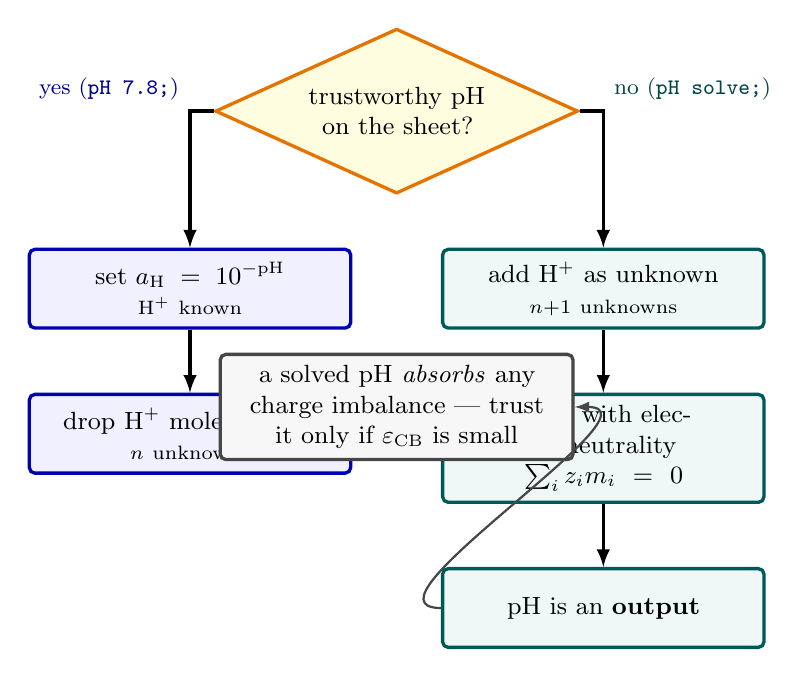
\begin{tikzpicture}[
    node distance=8mm,
    box/.style={draw, very thick, rounded corners=2pt, align=center,
                font=\small, inner sep=4pt, minimum height=10mm,
                text width=38mm},
    q/.style={draw, very thick, fill=yellow!12, draw=orange!90!black,
              align=center, font=\small, inner sep=3pt,
              shape=diamond, aspect=2.2, text width=26mm},
    given/.style={box, draw=blue!70!black, fill=blue!6},
    solve/.style={box, draw=teal!70!black, fill=teal!6},
    flow/.style={->, >=latex, very thick},
]
\node[q] (q) {trustworthy pH\\ on the sheet?};
\node[given, below left=12mm and -6mm of q] (g1) {set $a_{\rm H}=10^{-\mathrm{pH}}$\\ \scriptsize H$^+$ known};
\node[given, below=of g1] (g2) {drop H$^+$ mole balance\\ \scriptsize $n$ unknowns};
\node[solve, below right=12mm and -6mm of q] (s1) {add H$^+$ as unknown\\ \scriptsize $n{+}1$ unknowns};
\node[solve, below=of s1] (s2) {close with electroneutrality\\ $\sum_i z_i m_i=0$};
\node[solve, below=of s2] (s3) {pH is an \textbf{output}};
\node[box, draw=gray!55!black, fill=gray!6, below=20mm of q,
      text width=42mm] (warn)
   {a solved pH \emph{absorbs} any charge imbalance --- trust it only if $\varepsilon_{\rm CB}$ is small};
\draw[flow] (q.west) -| node[above left, font=\footnotesize, text=blue!60!black]{yes (\code{pH 7.8;})} (g1.north);
\draw[flow] (q.east) -| node[above right, font=\footnotesize, text=teal!55!black]{no (\code{pH solve;})} (s1.north);
\draw[flow] (g1) -- (g2);
\draw[flow] (s1) -- (s2);
\draw[flow] (s2) -- (s3);
\draw[->, >=latex, thick, gray!55!black] (s3) to[out=180,in=0] (warn.east);
\end{tikzpicture}
\caption{The two ways the speciation solver closes the proton balance.
If a trustworthy pH is on the analysis (left, blue), H$^+$ is
\emph{known}: fix $a_{\rm H}=10^{-\mathrm{pH}}$ and drop its mole balance,
leaving $n$ unknowns.  If the pH is stale or missing (right, teal),
H$^+$ becomes an extra unknown and \emph{electroneutrality}
$\sum_i z_i m_i=0$ supplies the missing equation---the pH then falls out as
an output, exactly as a titration determines it physically.  The caveat
(grey): a solved pH silently absorbs any charge-balance error in the input,
so it is only as good as $\varepsilon_{\rm CB}$.}
\label{fig:ph-closures}
\end{figure}


\paragraph{pH given.}  If a trustworthy pH is on the sheet, set
\begin{equation}
   a_{\rm H} \;=\; 10^{-\mathrm{pH}},
   \label{eq:ph-given}
\end{equation}
treat $\text{H}^+$ as \emph{known}, and remove its mole balance from the
system: $\text{H}^+$ (and the $\text{OH}^-$ that chains off it) are
simply algebraic functions of the fixed $a_{\rm H}$.  The unknowns stay
the $n$ master molalities.  This is the dict form \dict{pH 7.8;}.

\paragraph{pH solved (electroneutrality).}  Often the reported pH is
stale, drifted in the sample bottle, or simply missing.  Then
$\text{H}^+$ becomes an \emph{extra unknown} and an extra equation must
replace its missing total.  That equation is \emph{electroneutrality}: a
real solution carries no net charge,
\begin{equation}
   \boxed{\;
   \sum_i z_i\,m_i \;=\; 0
   \;}
   \label{eq:electroneutrality}
\end{equation}
summed over \emph{all} species --- masters, $\text{H}^+$, $\text{OH}^-$,
and every complex.  The pH is then an \emph{output}: the free
$\text{H}^+$ adjusts until the cations and anions balance.  This is the
dict form \dict{pH solve;}.

\begin{intuition}
Charge balance closing the pH is exactly what a titration does
physically.  When the cation and anion totals on a sheet do not add up to
zero charge, something is wrong --- a missing analyte, a unit slip, an
alkalinity mis-reported --- and the \emph{solved} pH silently
\emph{absorbs} that error: it moves $\text{H}^+$ (and hence
$\text{OH}^-$, $\text{HCO}_3^-$, $\text{CO}_3^{2-}$) to make the books
balance.  A solved pH is only as trustworthy as the charge balance of the
analysis behind it.  That is why the next subsection insists on measuring
the imbalance \emph{before} believing the answer.
\end{intuition}

\subsection{The PHREEQC percent-error convention}

A defensible speciation report must say how far the input was from charge
balance.  Following PHREEQC \cite{Parkhurst2013}, Choupo reports the
\emph{charge-balance percent error}
\begin{equation}
   \boxed{\;
   \varepsilon_{\rm CB} \;=\; 100 \cdot
   \frac{\bigl|\,S_+ - S_-\,\bigr|}{\tfrac12\,(S_+ + S_-)}
   \;=\; 200 \cdot
   \frac{\bigl|\,S_+ - S_-\,\bigr|}{S_+ + S_-},
   \;}
   \label{eq:percent-error}
\end{equation}
where $S_+ = \sum_{z_j>0} |z_j|\,T_j$ and $S_- = \sum_{z_j<0}
|z_j|\,T_j$ are the cation and anion \emph{equivalent} sums over the
\emph{master totals} ($\text{H}^+/\text{OH}^-$ are not part of a water
analysis, so they are excluded).  The factor 200 (not 100) normalises by
the \emph{average} of the two sums, so a $+5$\,\% cation excess and a
$-5$\,\% anion deficit each register as the same $\approx 5$\,\%.  Choupo
prints $\varepsilon_{\rm CB}$ \emph{before} it solves, and when it
exceeds $\approx 5$\,\% raises a loud advisory: the analysis is
internally inconsistent and the solved pH is not trustworthy because it
has absorbed the lab error.  This is the simulator's no-silent-crutch
rule applied to data quality --- the user is told what the number is
carrying.

\subsection{The solution algorithm: Newton in log-molality}

\begin{figure}[ht]
\centering
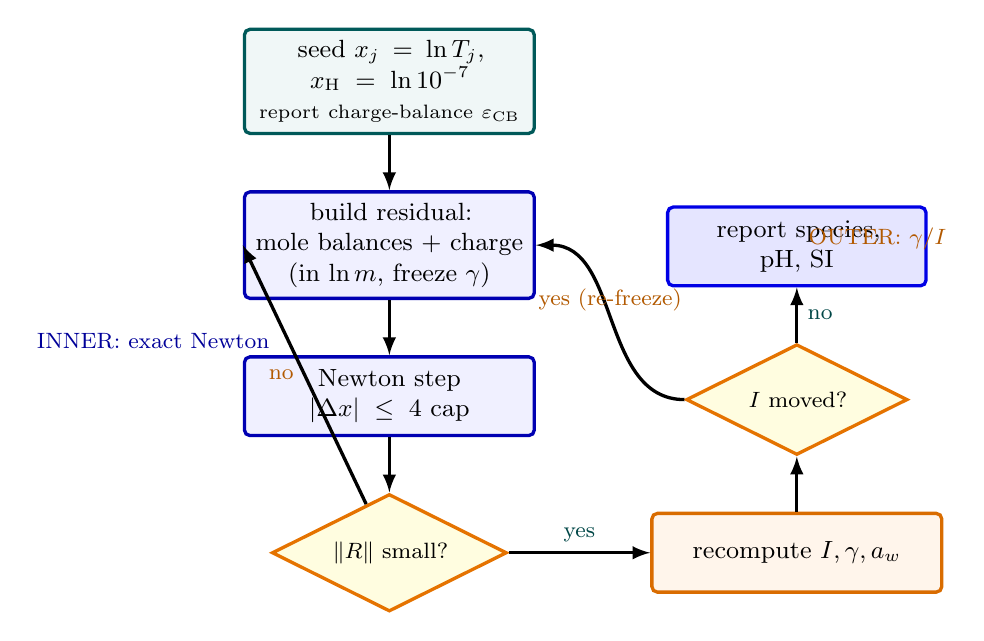
\begin{tikzpicture}[
    node distance=7mm,
    stp/.style={draw, very thick, rounded corners=2pt, align=center,
                 font=\small, inner sep=4pt, minimum height=10mm,
                 text width=34mm},
    init/.style={stp, draw=teal!70!black, fill=teal!6},
    inner/.style={stp, draw=blue!70!black, fill=blue!6},
    outer/.style={stp, draw=orange!85!black, fill=orange!8},
    dec/.style={draw, very thick, fill=yellow!12, draw=orange!90!black,
                align=center, font=\footnotesize, inner sep=2pt,
                shape=diamond, aspect=2, text width=20mm},
    flow/.style={->, >=latex, very thick},
]
\node[init] (seed) {seed $x_j=\ln T_j$, $\;x_{\rm H}=\ln10^{-7}$\\ \scriptsize report charge-balance $\varepsilon_{\rm CB}$};
\node[inner, below=of seed] (build) {build residual:\\ mole balances $+$ charge\\ (in $\ln m$, freeze $\gamma$)};
\node[inner, below=of build] (newton) {Newton step\\ $|\Delta x|\le 4$ cap};
\node[dec, below=of newton] (conv) {$\|R\|$ small?};
\node[outer, right=18mm of conv] (gamma) {recompute $I,\gamma,a_w$};
\node[dec, above=of gamma] (Iconv) {$I$ moved?};
\node[stp, draw=blue!90!black, fill=blue!10, above=of Iconv,
      text width=30mm] (done) {report species, pH, SI};
\draw[flow] (seed) -- (build);
\draw[flow] (build) -- (newton);
\draw[flow] (newton) -- (conv);
\draw[flow] (conv) -- node[left, font=\footnotesize, text=orange!70!black]{no} (build.west);
\draw[flow] (conv.east) -- node[above, font=\footnotesize, text=teal!55!black]{yes} (gamma.west);
\draw[flow] (gamma) -- (Iconv);
\draw[flow] (Iconv.west) to[out=180,in=0]
   node[above, font=\footnotesize, text=orange!70!black]{yes (re-freeze)} (build.east);
\draw[flow] (Iconv) -- node[right, font=\footnotesize, text=teal!55!black]{no} (done);
\node[font=\footnotesize, text=blue!60!black] at (-3.0,-3.3)
   {INNER: exact Newton};
\node[font=\footnotesize, text=orange!70!black] at (6.2,-2.0)
   {OUTER: $\gamma/I$};
\end{tikzpicture}
\caption{The speciation solver as a two-loop machine---the same
freeze-the-slow-coupling pattern as a recycle tear.  The \emph{inner} loop
(blue) is an exact Newton on the mole balances (plus electroneutrality when
the pH is solved), written in $\ln m$ so molalities stay positive and the
mass-action laws turn linear; each step is capped at $|\Delta x|\le4$ so
the iteration cannot leap out of its basin.  The \emph{outer} loop (orange)
freezes the activity coefficients, solves the inner system exactly, then
re-evaluates $\gamma$ and $a_w$ at the new ionic strength, repeating until
$I$ stops moving.  Before any of it runs, the charge-balance error
$\varepsilon_{\rm CB}$ is reported (teal)---a solved pH is no better than
the analysis it balances.}
\label{fig:speciation-solver}
\end{figure}


The mole balances~\eqref{eq:spec-molebalance} are stiff: molalities span
many orders of magnitude ($\text{Na}^+$ at $10^{-2}$, $\text{CO}_3^{2-}$
at $10^{-5}$, $\text{H}^+$ at $10^{-8}$) and must stay strictly positive.
Both problems vanish under the substitution
\begin{equation}
   x_j \;\equiv\; \ln m_j
   \qquad\Longrightarrow\qquad
   m_j = e^{x_j} > 0 \;\;\text{automatically},
   \label{eq:spec-logvar}
\end{equation}
and the mass-action law~\eqref{eq:spec-massaction} becomes \emph{linear}
in the log unknowns:
\begin{equation}
   \ln m_s \;=\; \ln 10\,\log_{10}K_s - \ln\gamma_s
   + \nu_{s,\mathrm{H_2O}}\ln a_w
   + \sum_j \nu_{sj}\bigl(\ln\gamma_j + x_j\bigr).
   \label{eq:spec-logmassaction}
\end{equation}
The residual vector is the set of mole balances (plus, when $\text{H}^+$
is solved, the electroneutrality row~\eqref{eq:electroneutrality} with
$x_{\rm H}$ as its unknown).  Because each $m_s$ depends on $x_j$ through
\eqref{eq:spec-logmassaction}, the Jacobian is \emph{analytic}: a
mole-balance row has $\partial R_j/\partial x_k = -\delta_{jk}\,m_j -
\sum_s \nu_{sj}\nu_{sk}\,m_s$, and the dense $n\times n$ (or
$(n{+}1)\times(n{+}1)$) system is solved by Gaussian elimination
(Chapter~\ref{ch:nrND}).  Newton steps in $\ln m$ are capped at
$|\Delta x|\le 4$ ($m$ may change by at most $e^4\!\approx\!55\times$ per
step) so the iteration cannot leap out of the basin.

The activity coefficients are the wrinkle: $\gamma_j$ depends on the
ionic strength $I=\tfrac12\sum_i z_i^2 m_i$, which depends on the very
molalities being solved.  Choupo breaks this with a
\emph{frozen-$\gamma$ fixed point}: hold all $\gamma$ (and the water
activity $a_w$) constant, run Newton to convergence on the molalities,
recompute $I$, $\gamma$ and $a_w$, and repeat the outer pass until $I$
stops moving.  The two-loop structure --- an outer $\gamma/I$
self-consistency wrapping an inner exact Newton --- is the same pattern
used for the recycle tear (Chapter~\ref{ch:newton-tears}): freeze the slow
coupling, solve the fast system exactly, update, repeat.

\begin{keyidea}
Speciation is solved as a \textbf{two-loop} problem.  The \emph{inner}
loop is an exact Newton on mole balances (and electroneutrality, if pH is
solved) written in $\ln m$ so molalities stay positive and the
mass-action laws become linear.  The \emph{outer} loop freezes the
activity coefficients and water activity, then re-evaluates them at the
new ionic strength --- iterating $I \to \gamma \to m \to I$ to
self-consistency.  The default $\gamma$ model is Davies (the teaching
rung below Pitzer); Pitzer HMW is selectable for high ionic strength.
\end{keyidea}

\subsection{The Davies equation: a parameter-free single-ion
\texorpdfstring{$\gamma_i$}{gamma}}\label{sec:davies}

\begin{figure}[ht]
\centering
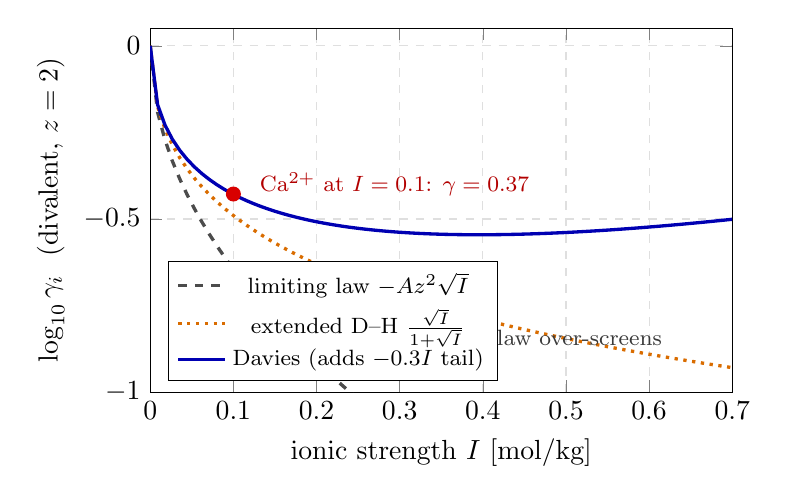
\begin{tikzpicture}
\begin{axis}[
    width=0.74\linewidth, height=6.2cm,
    xlabel={ionic strength $I$ [mol/kg]},
    ylabel={$\log_{10}\gamma_i$ \ (divalent, $z=2$)},
    xmin=0, xmax=0.7,
    ymin=-1.0, ymax=0.05,
    grid=major,
    grid style={gray!25, dashed},
    legend pos=south west,
    legend style={font=\footnotesize},
]
\addplot[domain=0:0.7, samples=80, gray!60!black, very thick, dashed]
   ({x},{-0.51*4*sqrt(x)});
\addlegendentry{limiting law $-Az^2\sqrt I$}
\addplot[domain=0:0.7, samples=80, orange!85!black, very thick, dotted]
   ({x},{-0.51*4*sqrt(x)/(1+sqrt(x))});
\addlegendentry{extended D--H $\frac{\sqrt I}{1+\sqrt I}$}
\addplot[domain=0:0.7, samples=80, blue!70!black, very thick]
   ({x},{-0.51*4*(sqrt(x)/(1+sqrt(x)) - 0.3*x)});
\addlegendentry{Davies (adds $-0.3I$ tail)}
\addplot[only marks, mark=*, mark size=2.5pt, mark options={red!85!black}]
   coordinates {(0.10, -0.428)};
\node[font=\footnotesize, text=red!70!black, anchor=west]
   at (axis cs:0.12,-0.40) {Ca$^{2+}$ at $I=0.1$: $\gamma=0.37$};
\node[font=\footnotesize, text=gray!45!black, anchor=west]
   at (axis cs:0.30,-0.85) {limiting law over-screens};
\end{axis}
\end{tikzpicture}
\caption{The three rungs of single-ion non-ideality for a divalent ion,
showing why Davies is the right teaching default.  The bare Debye--H\"uckel
limiting law (dashed grey) over-screens at finite $I$, driving
$\gamma$ unphysically low.  The extended law's closest-approach denominator
$1+\sqrt I$ (dotted orange) tames it.  Davies (blue) adds one universal,
salt-\emph{in}dependent empirical tail $-0.3I$ that turns the decline back
upward---mimicking the short-range repulsion a per-salt $\beta^{(0)}$ would
otherwise carry, with \emph{no} fitted parameter.  At
$I=0.1$ the worked Ca$^{2+}$ value (red, $\gamma=0.37$) sits 40\,\% above
the limiting-law answer---exactly the gap that decides whether
CaCO$_3$ reads as supersaturated at a membrane wall.}
\label{fig:davies-vs-dh}
\end{figure}


The speciation network of the previous subsections needs, for every
charged species, a \emph{single-ion} activity coefficient $\gamma_i$ ---
not the mean $\gamma_\pm$ that the eNRTL (\S\ref{ch:enrtl}) and the
osmotic Pitzer (\S\ref{ch:electrolytes}) deliver.  The cheapest rung that
still gets the electrostatics right is the \emph{Davies equation}
\cite{Davies1962}, the model Choupo's \code{davies} kernel
(\code{AqueousActivity}) implements and the speciation solver freezes
once per outer iteration.  This subsection derives it, states exactly
what the code evaluates, and is honest about where it runs out.

\paragraph{From the limiting law to Davies.}  The Debye--H\"uckel theory
(1923) treats each ion as a point charge surrounded by a diffuse
\emph{ionic atmosphere} of opposite net charge.  Solving the linearised
Poisson--Boltzmann equation for the work of charging that atmosphere
gives the celebrated \emph{limiting law}, valid only as $I\to 0$,
\begin{equation}
   \log_{10}\gamma_i \;=\; -A\,z_i^{2}\sqrt I ,
   \label{eq:dh-limiting}
\end{equation}
where the square-root in ionic strength $I=\tfrac12\sum_i m_i z_i^2$ is
the electrostatic signature no mole-fraction polynomial can reproduce.
The slope $A$ is a property of the \emph{solvent only} (no salt-specific
input).  The limiting law over-screens at finite concentration; the
\emph{extended} Debye--H\"uckel law tames it with a closest-approach
denominator $1+\mathring{a}B\sqrt I$, and the \textbf{Davies} fix takes
the universal choice $\mathring{a}B=1$ and adds a single empirical
linear tail $-0.3\,I$ that turns the otherwise monotone decline back
upward, mimicking the short-range repulsion that a per-salt
$\beta^{(0)}$ would otherwise carry:
\begin{equation}
   \boxed{\;
   \log_{10}\gamma_i \;=\; -\,A\,z_i^{2}
   \left(\frac{\sqrt I}{1+\sqrt I} \;-\; 0.3\,I\right).
   \;}
   \label{eq:davies}
\end{equation}
The remarkable thing about \eqref{eq:davies} is that it carries
\emph{no adjustable, salt-specific parameter at all} --- only $A$ (the
solvent) and the ion charge $z_i$.  That is its entire pedagogical and
practical appeal: a defensible $\gamma_i$ for \emph{any} ion in water
from charge alone.

\paragraph{The slope $A$ and its temperature scaling.}  $A$ is the
$\log_{10}$-base Debye--H\"uckel slope; Choupo anchors it at the
textbook
\[
   A \;=\; 0.51~\mathrm{kg^{1/2}\,mol^{-1/2}} \quad(25\,\textdegree\mathrm C),
\]
which is exactly $3A_\phi/\ln 10$ with the Pitzer $A_\phi=0.3915$, so the
Davies and Pitzer rungs share one consistent Debye--H\"uckel
constant.  Off 25\,\textdegree C, $A$ inherits its temperature
dependence from the \emph{solvent} through
\begin{equation}
   A(T) \;=\; 0.51 \times f_{\rm DH}(T),
   \qquad
   f_{\rm DH}(T) =
   \left(\frac{\rho_w(T)}{\rho_w^{25}}\right)^{\!1/2}
   \left(\frac{\varepsilon_w^{25}\,T_{25}}{\varepsilon_w(T)\,T}\right)^{\!3/2},
   \label{eq:davies-AT}
\end{equation}
the same dimensionless factor (\code{SolventProperties::debye\-Huckel\-Factor})
that scales the Pitzer $A_\phi$ and the eNRTL $A_{\rm DH}$ --- so the
three electrolyte kernels move together with temperature, never
independently.  The factor is built from the static permittivity
$\varepsilon_w(T)$ (Malmberg--Maryott \cite{MalmbergMaryott1956}) and the
density $\rho_w(T)$ (Kell \cite{Kell1975}), each written as a
\emph{ratio} anchored so that $f_{\rm DH}(298.15\,\mathrm K)\equiv 1$: at
25\,\textdegree C the value is byte-identically $A=0.51$, and only off
25\,\textdegree C does the physics of a colder, denser, more polar
solvent (a \emph{larger} $A$, hence stronger non-ideality) appear.  The
$T^{-3/2}\varepsilon^{-3/2}$ form is the textbook Debye--H\"uckel scaling
of the charging integral.

\paragraph{What the code actually evaluates.}  The \code{davies} kernel
is deliberately tiny and glass-box (\code{AqueousActivity::evaluate}):
\begin{itemize}[leftmargin=*,nosep,topsep=2pt]
  \item it computes $A=0.51\,f_{\rm DH}(T)$ once, then returns a closure
        $\gamma(z)=10^{-A z^2(\sqrt I/(1+\sqrt I)-0.3I)}$ evaluated with
        \code{std::pow(10.0,...)} (not $e^{x\ln 10}$, to keep the golden
        masters byte-stable);
  \item \textbf{neutral species} ($z=0$) and the $I\le 0$ guard return
        $\gamma=1$ exactly --- there is \emph{no} Setchenow
        salting-out term ($\log_{10}\gamma_{\rm neutral}=b\,I$) in this
        rung, stated honestly rather than faked;
  \item it is a pure function of $(|z|,I,A)$, so the solver freezes the
        whole $\gamma$ table at the iteration's $I$ (the Newton in
        log-molality stays linear in the activities --- see the solution
        algorithm above).
\end{itemize}

\begin{example}[Davies vs.\ the limiting law for Ca\textsuperscript{2+}]
Take a brackish water at $I=0.10$\,mol/kg, 25\,\textdegree C, so
$A=0.51$ and $\sqrt I=0.316$.  For a divalent ion ($z=2$, $z^2=4$):
\[
   \frac{\sqrt I}{1+\sqrt I}-0.3I
   = \frac{0.316}{1.316}-0.030 = 0.240-0.030 = 0.210,
\]
\[
   \log_{10}\gamma_{\rm Ca} = -0.51\times 4 \times 0.210 = -0.428,
   \qquad \gamma_{\rm Ca}=10^{-0.428}=0.373.
\]
The bare limiting law \eqref{eq:dh-limiting} would give
$\log_{10}\gamma=-0.51\times4\times0.316=-0.645$, i.e.\
$\gamma=0.226$ --- a \emph{40\,\% lower} activity coefficient.  The
denominator and the $-0.3I$ tail together pull the divalent ion back
from the unphysically strong screening the limiting law predicts; this
is precisely the difference that decides whether CaCO\textsubscript{3}
shows up as supersaturated (\eqref{eq:spec-SI}) at the membrane wall.
A monovalent ion at the same $I$ has only a quarter of the exponent,
$\gamma_{\rm Na}=10^{-0.107}=0.78$ --- the $z^2$ weighting in action.
\end{example}

\paragraph{Power and limit.}  \emph{Power:} a single, parameter-free
equation gives every ion a defensible $\gamma_i$ from its charge alone,
with the correct $\sqrt I$ electrostatic limit and a sensible turn-up at
moderate $I$ --- the ideal teaching rung between ``ideal solution''
($\gamma_i=1$) and a fully fitted Pitzer.  \emph{Limit:} the $-0.3I$ tail
is empirical, so Davies is trustworthy only to $I\approx 0.5$\,mol/kg;
the speciation solver therefore raises an explicit advisory once
$I$ exceeds $\approx 0.7$\,mol/kg and points the student at the
multi-ion Pitzer HMW kernel (\S\ref{ch:pitzer-hmw},
\cite{Pitzer1973}), which carries the salt-specific virial coefficients
Davies lacks.  Neutral species are ideal ($\gamma=1$), and the
calorimetric ($T$-derivative) accuracy of the slope is only as good as
the solvent correlations \eqref{eq:davies-AT}.  The model is honest about
all three.

\subsection{Activity model and water activity}

The default single-ion $\gamma$ is the Davies equation
\eqref{eq:davies} of \S\ref{sec:davies}, with $A\approx 0.51$ at
25\,\textdegree C and the $\varepsilon_w(T),\rho_w(T)$ scaling
\eqref{eq:davies-AT} shared with the Pitzer kernel; it is trustworthy to
$I\approx 0.5$\,mol/kg, the solver raises an advisory above $I\approx
0.7$, and Pitzer HMW \cite{Pitzer1973} is the documented replacement.
Neutral species take $\gamma=1$.  The water activity is
\begin{equation}
   \ln a_w \;=\; -\,M_w\,\phi\sum_i m_i,
   \label{eq:spec-aw}
\end{equation}
with $M_w$ the molar mass of water in kg/mol and $\phi$ the osmotic
coefficient --- the definition~\eqref{eq:phi-def}.  Under \textbf{Davies}
the solver keeps the dilute approximation $\phi=1$ (declared in the run
header), consistent with Davies being indicative beyond $I\approx
0.5$\,mol/kg.  Under \textbf{Pitzer} $\phi$ is the \emph{real} multi-ion
osmotic coefficient of \eqref{eq:hmw-osmotic}, built from the same
virials as the $\gamma_i$, so the brine's water activity --- the gypsum
$a_w^2$ leg, the boiling-point elevation, the osmotic pressure --- is
Pitzer-consistent and not a $\phi=1$ guess (\S\ref{sec:hmw-osmotic}).

\subsection{Temperature dependence of \texorpdfstring{$K$}{K}}

Formation constants are anchored at 25\,\textdegree C and corrected to
the run temperature by a three-tier priority, \emph{all} pinned so that
$\log_{10}K(298.15\,\mathrm K)\equiv\log_{10}K_{25}$ exactly (the
25\,\textdegree C run is byte-stable by construction):
\begin{enumerate}[leftmargin=*,nosep,topsep=2pt]
  \item \textbf{Analytic} (PHREEQC \code{-analytical\_expression}): the
        fitted shape $\mathrm{ana}(T)=A_1 + A_2 T + A_3/T + A_4\log_{10}T
        + A_5/T^2 + A_6 T^2$ is applied as an \emph{anchored} correction,
        $\log_{10}K(T)=\log_{10}K_{25} + [\mathrm{ana}(T) -
        \mathrm{ana}(298.15)]$, so the published fit's absolute offset
        cancels and only its $T$-shape is borrowed; outside the fitted
        range the run announces ``$K(T)$ extrapolated'' (no silent
        extrapolation).
  \item \textbf{van't Hoff} (constant $\Delta H_{\rm r}$):
        $\log_{10}K(T)=\log_{10}K_{25} + \dfrac{\Delta H_{\rm r}}{\Rgas\ln
        10}\!\left(\dfrac{1}{298.15}-\dfrac{1}{T}\right)$.
  \item \textbf{Flat}: a genuinely bare entry holds $K$ at its
        25\,\textdegree C value.
\end{enumerate}
Each form is listed at verbosity $\ge 2$, so the student sees exactly
which constants were temperature-corrected and how.

\subsection{Open systems: the Henry gas pin}\label{sec:gaspin}

Everything above conserves every master total --- a \emph{closed}
vessel.  A water in contact with a large gas reservoir (the atmosphere,
a blanketing gas) obeys a different constraint: the dissolved gas is
set by gas--liquid equilibrium, not by an inventory.  Henry's law fixes
the \emph{activity} of the dissolved species,
%
\begin{equation}
  a_{\mathrm{dissolved}} \;=\; K_H(T)\, p_{\mathrm{gas}},
  \label{eq:gaspin}
\end{equation}
%
with $K_H$ from the gas--liquid catalogue
(\file{chemistry/gasLiquid/}, PHREEQC \code{PHASES} form, $\log_{10}
K_H$ anchored and $T$-corrected exactly like every other constant of
the previous subsection).  The case declares the reservoir per gas:
%
\begin{verbatim}
atmosphere { pCO2 4.2e-4 atm;  O2 0.2095 atm;  N2 0.7808 atm; }
\end{verbatim}
%
\noindent\textbf{The swap.}  For each listed gas the solver drops ONE
mole balance and puts equation~\eqref{eq:gaspin} in its place --- in
log space, $\ln a_{\mathrm{dissolved}} = \ln K_H + \ln p$, which is
\emph{linear} in the unknowns $x_j=\ln m_j$, so Newton absorbs it
without ceremony.  Which balance is dropped follows from what the gas
dissolves \emph{into}:
\begin{itemize}[leftmargin=*,nosep,topsep=2pt]
  \item a \textbf{computed species} --- $\mathrm{CO_2(g)}$ dissolves to
        $\mathrm{CO_2(aq)}$, a mass-action species formed from the
        $\mathrm{HCO_3^-}$ master: the \emph{family's} balance
        ($\mathrm{HCO_3^-}$) is replaced, and the whole carbonate
        ladder equilibrates with the reservoir.  Total dissolved
        carbon becomes a solved \emph{outcome}; the \code{totals}
        entry is only the initial guess (announced, and excluded from
        the charge-imbalance check --- a guess is not an analysis);
  \item an \textbf{inert neutral master} --- $\mathrm{O_2}$,
        $\mathrm{N_2}$, $\mathrm{CH_4}$, $\mathrm{H_2}$ dissolve to
        themselves (identity records in \file{species/aqueous.dat},
        charge 0): the pin replaces the master's \emph{own} balance
        and the dissolved concentration is set by the gas phase alone.
\end{itemize}
Several gases pin simultaneously (one row each; two gases claiming the
same master are refused).  A gas whose dissolution spans several
aqueous legs at once --- $\mathrm{H_2S(g)} = \mathrm{H^+} +
\mathrm{HS^-}$, because the neutral $\mathrm{H_2S(aq)}$ species is not
yet curated --- is refused loudly as a named gap rather than pinned
approximately.

Two textbook numbers fall out of pure water open to air with no
fitting anywhere (\file{rainwater\_air}): carbonic acid from
420\,ppm $\mathrm{CO_2}$ alone gives rain its natural
$\mathrm{pH}\approx 5.6$, and the dissolved-oxygen saturation runs
retrograde with temperature --- ${\sim}8.5$\,mg/L at
25\,\textdegree C rising to ${\sim}11$\,mg/L at 10\,\textdegree C ---
which is why cold streams hold more oxygen than warm ones.

\subsection{From speciation to saturation: the scaling link}

\begin{figure}[ht]
\centering
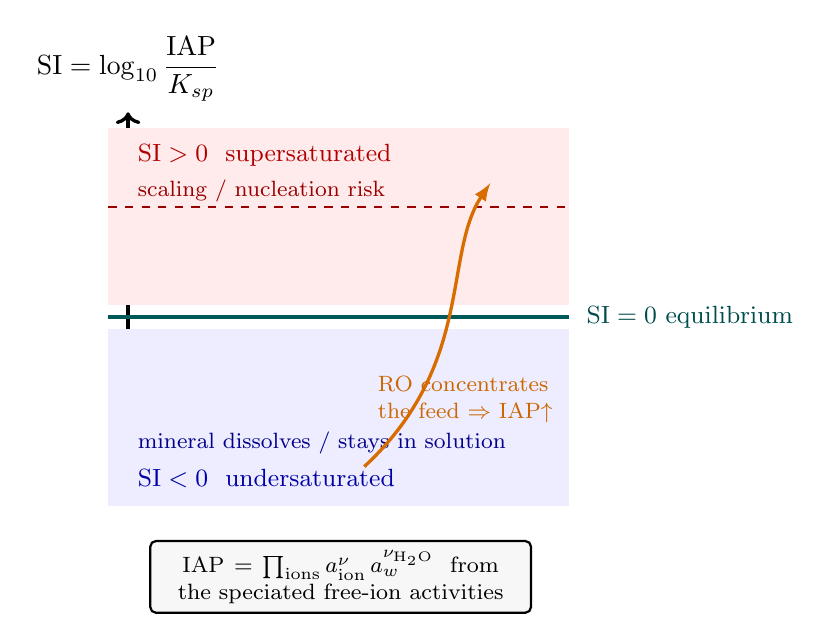
\begin{tikzpicture}[
    flow/.style={->, >=latex, very thick},
]
\draw[->, very thick] (0,-2.4) -- (0,2.6)
   node[anchor=south]{$\mathrm{SI}=\log_{10}\dfrac{\mathrm{IAP}}{K_{sp}}$};
\fill[red!8] (-0.25,0.15) rectangle (5.6,2.4);
\fill[blue!7] (-0.25,-0.15) rectangle (5.6,-2.4);
\draw[very thick, teal!70!black] (-0.25,0) -- (5.6,0);
\node[teal!60!black, font=\small, anchor=west] at (5.7,0) {$\mathrm{SI}=0$ equilibrium};
\draw[red!60!black, thick, dashed] (-0.25,1.4) -- (5.6,1.4);
\node[red!70!black, font=\small, anchor=west] at (0.0,2.05) {$\mathrm{SI}>0$ \ supersaturated};
\node[red!60!black, font=\footnotesize, anchor=west] at (0.0,1.6) {scaling / nucleation risk};
\node[blue!65!black, font=\small, anchor=west] at (0.0,-2.05) {$\mathrm{SI}<0$ \ undersaturated};
\node[blue!55!black, font=\footnotesize, anchor=west] at (0.0,-1.6) {mineral dissolves / stays in solution};
\draw[flow, orange!85!black] (3.0,-1.9) .. controls (4.4,-0.6) and (4.0,0.8) .. (4.6,1.7);
\node[orange!80!black, font=\footnotesize, anchor=west, align=left]
   at (3.05,-1.05) {RO concentrates\\ the feed $\Rightarrow$ IAP$\uparrow$};
\node[draw, thick, rounded corners=2pt, fill=gray!6, font=\footnotesize,
      align=center, text width=46mm] at (2.7,-3.3)
   {$\mathrm{IAP}=\prod_{\rm ions} a_{\rm ion}^{\nu}\,a_w^{\nu_{\rm H_2O}}$ \ from the speciated free-ion activities};
\end{tikzpicture}
\caption{The saturation index turns speciated free-ion activities into a
single scaling verdict.  Once the solver knows every free-ion activity, the
ion-activity product IAP is compared to the solubility product $K_{sp}(T)$:
$\mathrm{SI}=\log_{10}(\mathrm{IAP}/K_{sp})$.  Below the teal equilibrium
line the mineral is undersaturated (blue, it dissolves or stays dissolved);
above it the water is supersaturated (red, scaling and nucleation risk).
As a reverse-osmosis stage concentrates the feed the activities climb and
the operating point walks \emph{up} the ladder (orange)---the
\code{scalingScan} op traces exactly this trajectory, and the
\code{equilibrate} option drops the precipitate once a mineral crosses
$\mathrm{SI}=0$.}
\label{fig:saturation-index}
\end{figure}


Once the free-ion activities are known, the \emph{saturation index} of
any mineral in \file{minerals.dat} follows immediately:
\begin{equation}
   \mathrm{SI} \;=\; \log_{10}\!\frac{\mathrm{IAP}}{K_{sp}(T)},
   \qquad
   \mathrm{IAP} = \prod_{\rm ions} a_{\rm ion}^{\nu}\;a_w^{\nu_{\rm H_2O}},
   \label{eq:spec-SI}
\end{equation}
$\mathrm{SI}<0$ undersaturated, $=0$ at equilibrium, $>0$ supersaturated
(scaling risk).  The \code{scalingScan} op walks this index along an RO
concentration trajectory; the \code{equilibrate} option goes further and
finds the precipitated amounts by an \emph{active-set} complementarity
solve (admit the most-supersaturated phase, drive its $\mathrm{SI}$ to
zero, evict any phase whose precipitated amount goes negative) layered on
top of exactly the Newton above.  Saturation indices are the bridge from
the chemistry of this section to the membrane and crystalliser chapters.

\paragraph{Power and limit.}  The power: from seven total
concentrations and a temperature the model recovers the entire
distribution of dozens of species, a defensible pH (closed by physics,
not by a stale measurement), and the saturation state of every candidate
scale mineral --- the same calculation a regulatory water-chemistry
report rests on, with every $\log K$, every $\gamma$, and every Newton
iteration visible.  The limits are deliberate and announced: the Davies
default is trustworthy only to $I\approx 0.5$\,mol/kg (use Pitzer
beyond); the water activity uses the $\phi=1$ dilute approximation;
neutral species are ideal ($\gamma=1$); a solved pH is no better than the
charge balance of its input, which is precisely why $\varepsilon_{\rm
CB}$ is reported and gated before the answer is offered.

\begin{example}[A brackish RO feed, pH solved]
A brackish feed lists (mg/L) Ca~84, Mg~27, Na~363, K~12, Cl~510,
SO\textsubscript{4}~250, HCO\textsubscript{3}~183 at 25\,\textdegree C,
with no reliable pH.  Run with \dict{pH solve;}.  The solver first
reports the charge-balance error $\varepsilon_{\rm CB}=200\,|S_+ -
S_-|/(S_+ + S_-)$ over the master equivalents; here it is a couple of
percent (a clean analysis), well under the $5$\,\% advisory.  It then
seeds $x_j=\ln T_j$, $x_{\rm H}=\ln 10^{-7}$, freezes Davies $\gamma$ at
the initial $I$, and Newton-solves the seven mole balances plus
electroneutrality in $\ln m$; recomputing $I$ and $\gamma$ and re-solving
a few times lands $I\approx 0.03$\,mol/kg and a solved
$\mathrm{pH}\approx 7.72$ --- close to the lab's reported 7.8, the charge
balance vindicating the analysis.  The carbonate now distributes into
$\text{HCO}_3^-$, $\text{CO}_3^{2-}$ and $\text{CaHCO}_3^+$, and the
calcite SI from \eqref{eq:spec-SI} reads the scaling risk that drives the
downstream RO audit
(\file{tutorials/props/electrolyte/scaling\_ro\_brackish}).
\end{example}

\begin{tutoriallink}
\file{tutorials/props/electrolyte/scaling\_ro\_brackish} --- the worked
feed above, with analytic ``pins'' (pure-water $K_w$, gypsum-saturated
CaSO\textsubscript{4}, neutral pure water) that nail the solver against
hand-checkable answers, then the feed speciated with \dict{pH solve;} and
a closed-vs-open-CO\textsubscript{2} scaling scan.
\file{tutorials/props/electrolyte/softener\_brackish} adds Gaines--Thomas
cation exchange on the same Newton.
\end{tutoriallink}

% ---------------------------------------------------------------------
\section{Fugacity and the vapour phase}\label{ch:fugacity}

\begin{whatyoulllearn}
The activity coefficient $\gamma_i$ of the previous chapter
corrects the liquid-side chemical potential for non-ideality.  On
the vapour side, the analogous correction is the
\emph{fugacity coefficient} $\varphi_i$.  Together $(\gamma_i,
\varphi_i)$ are the two multiplicative gauges that take the
ideal-mixture reference of Chapter~\ref{ch:ideal-mixing} all the way
to real-fluid phase equilibrium. fixes $\varphi_i = 1$
(ideal-gas vapour), which is adequate at the operating pressures of
the shipped tutorials; the cubic equations of state that produce
$\varphi_i \neq 1$ at higher pressures are on the v1.x roadmap.
\end{whatyoulllearn}

\subsection{Why we need fugacity at all}

The chemical potential of a real gas is not $\mu = \mu^0(T) + RT \ln
(P/P_0)$.  That expression is the ideal-gas case where the molecules
do not interact.  Real molecules feel attractive and repulsive
forces; their chemical potential depends on more than just pressure
in a logarithmic-of-ratio way.

G.~N.~Lewis (1901) defined the \emph{fugacity} $f$ as the auxiliary
variable that restores the simple logarithmic form for any fluid:
\begin{equation}
   \boxed{\;
   \mu(T, P) \;=\; \mu^0(T) \;+\; RT \ln \frac{f(T, P)}{f^0}.
   \;}
   \label{eq:fugacity-def}
\end{equation}
Reference $f^0 = 1$ bar by convention.  The defining condition is
that $f \to P$ as $P \to 0$: in the dilute-gas limit, the fugacity
becomes the ordinary pressure.  The \emph{fugacity coefficient} is
the ratio
\begin{equation}
   \varphi(T, P) \;\equiv\; \frac{f(T, P)}{P},
\end{equation}
with $\varphi \to 1$ as $P \to 0$ and $\varphi = 1$ identically for
an ideal gas at any $P$.  Deviations of $\varphi$ from unity measure
how far the real gas departs from the ideal-gas equation of state.

\begin{intuition}
Fugacity is the engineering trick that lets every formula derived
under the ideal-gas assumption survive in a real-gas world: replace
$P$ with $f$ everywhere and the algebra continues to apply.  All of
the complexity of non-ideal molecular interactions is bundled into
the single multiplicative correction $\varphi$, which is then
computed from an equation of state.  $\varphi < 1$ for fluids
dominated by attraction (compression denser than ideal); $\varphi
> 1$ for fluids dominated by repulsion (e.g.\ helium near $T_c$).
\end{intuition}

\subsection{Fugacity of a pure liquid}

For a pure substance at saturation $(T, P^{\mathrm{sat}}(T))$,
liquid and vapour coexist and their chemical potentials are equal,
so their fugacities are equal too:
\begin{equation}
   f^{\mathrm{L}}(T, P^{\mathrm{sat}}) \;=\;
   f^{\mathrm{V}}(T, P^{\mathrm{sat}}) \;=\;
   \varphi^{\mathrm{sat}}(T)\,P^{\mathrm{sat}}(T).
\end{equation}
For a pure liquid at a different $P$, the small pressure
dependence is the \emph{Poynting correction}
$\exp\!\bigl[v^{\mathrm{L}}(P - P^{\mathrm{sat}})/(RT)\bigr]$, which is
$\sim 1$ until $P$ exceeds several bar above $P^{\mathrm{sat}}$.
At operating conditions the simulator drops the Poynting
factor entirely:
\begin{equation}
   f^{\mathrm{L},*}_i(T) \;\approx\; \varphi_i^{\mathrm{sat}}(T)\,P_i^{\mathrm{sat}}(T).
   \label{eq:fugacity-pure-liq}
\end{equation}
With the ideal-gas $\varphi_i^{\mathrm{sat}} = 1$ assumption, this
collapses further to $f^{\mathrm{L},*}_i \approx P_i^{\mathrm{sat}}$.

\subsection{Partial fugacity in mixtures}

For component $i$ in a mixture, the partial fugacity $\hat f_i$
plays the role of an ``effective partial pressure''.  In a gas
mixture
\begin{equation}
   \hat f_i^{\mathrm{V}}(T, P, \mathbf{y})
   \;=\; y_i\,\hat\varphi_i(T, P, \mathbf{y})\,P,
   \label{eq:fugacity-vap-mix}
\end{equation}
where $\hat\varphi_i$ is the partial fugacity coefficient of $i$ in
the mixture (note the hat: it depends on composition, unlike the
pure-component $\varphi_i$).  In an ideal-gas mixture
$\hat\varphi_i = 1$ for every $i$, recovering Dalton's law $\hat
f_i = y_i P$ that we already derived in
Chapter~\ref{ch:ideal-mixing}.

In a liquid mixture the partial fugacity is built from the
activity coefficient and the pure-component liquid fugacity:
\begin{equation}
   \hat f_i^{\mathrm{L}}(T, P, \mathbf{x})
   \;=\; x_i\,\gamma_i(T, \mathbf{x})\,f^{\mathrm{L},*}_i(T)
   \;\approx\; x_i\,\gamma_i\,\varphi_i^{\mathrm{sat}}\,P_i^{\mathrm{sat}}.
   \label{eq:fugacity-liq-mix}
\end{equation}
The two corrections separate cleanly: $\gamma_i$ absorbs
\emph{composition-driven} non-ideality (next-neighbour interactions
in the liquid); $\varphi_i^{\mathrm{sat}}$ absorbs the
\emph{vapour-phase} non-ideality at the saturation pressure of the
pure component.  In both are taken at the simplest end
($\gamma_i$ from NRTL/Wilson but $\varphi_i^{\mathrm{sat}} = 1$).

\subsection{Phase-equilibrium criterion in fugacity form}

Chapter~\ref{ch:three-pillars} laid out the criterion:
$\mu_i^{\mathrm{L}} = \mu_i^{\mathrm{V}}$ for every component
across the phase boundary.  Substituting \eqref{eq:fugacity-def}
into both sides and cancelling $\mu^0$ and $f^0$,
\begin{equation}
   \boxed{\;
   \hat f_i^{\mathrm{L}}(T, P, \mathbf{x})
   \;=\;
   \hat f_i^{\mathrm{V}}(T, P, \mathbf{y})
   \quad\text{for every component } i.
   \;}
   \label{eq:fugacity-equilibrium}
\end{equation}
Substituting \eqref{eq:fugacity-vap-mix} and
\eqref{eq:fugacity-liq-mix} produces the
\textbf{$\gamma$-$\varphi$ formulation}:
\begin{equation}
   x_i\,\gamma_i(\mathbf{x},T)\,\varphi_i^{\mathrm{sat}}(T)\,P_i^{\mathrm{sat}}(T)
   \;=\;
   y_i\,\hat\varphi_i(\mathbf{y},T,P)\,P.
   \label{eq:gamma-phi-here}
\end{equation}
This is the equation the manual's current Part~I Chapter~2 presents
out of context.  Now you can read it: liquid-side fugacity equals
vapour-side fugacity, both built up from the ideal-mixture baseline
($x_i$ or $y_i$ times a reference) times two real-fluid corrections
(the $\gamma$'s and the $\varphi$'s).

Setting $\hat\varphi_i = \varphi_i^{\mathrm{sat}} = 1$ (the ideal-gas-vapour assumption) reduces \eqref{eq:gamma-phi-here} to
\begin{equation}
   \boxed{\;
   x_i\,\gamma_i(\mathbf{x}, T)\,P_i^{\mathrm{sat}}(T)
   \;=\; y_i\,P.
   \;}
   \label{eq:modified-raoult}
\end{equation}
Often called \emph{modified Raoult's law}.  It is the closed-form
phase-equilibrium relation every flash, bubble-T, dew-T and
distillation stage  ultimately uses.  Setting $\gamma_i = 1$
on top gives plain Raoult.

\begin{figure}[ht]\centering
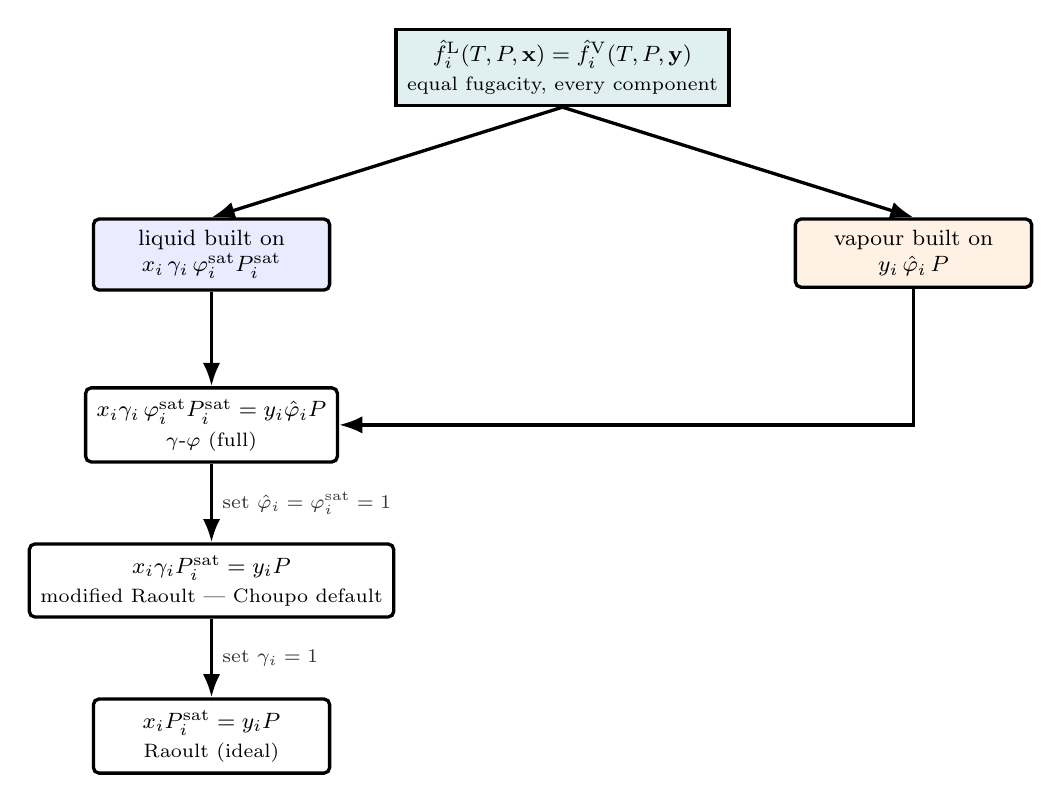
\begin{tikzpicture}[
    >={Latex[width=2.2mm]},
    box/.style ={draw, rounded corners=2pt, very thick, align=center,
                 inner sep=4pt, minimum width=30mm, font=\footnotesize},
    liq/.style ={box, fill=blue!8},
    vap/.style ={box, fill=orange!10},
    crit/.style={draw, very thick, align=center, inner sep=4pt,
                 fill=teal!12, minimum width=42mm, font=\footnotesize},
    flow/.style={->, very thick},
    lbl/.style ={font=\scriptsize, text=gray!40!black},
]
% top equilibrium criterion
\node[crit] (eq) {$\hat f_i^{\mathrm L}(T,P,\xv)=\hat f_i^{\mathrm V}(T,P,\yv)$\\[1pt]
                  {\scriptsize equal fugacity, every component}};
% liquid branch
\node[liq, below left=14mm and 8mm of eq] (lref)
     {liquid built on\\$x_i\,\gamma_i\,\varphi_i^{\mathrm{sat}}P_i^{\mathrm{sat}}$};
% vapour branch
\node[vap, below right=14mm and 8mm of eq] (vref)
     {vapour built on\\$y_i\,\hat\varphi_i\,P$};
% simplifications going down the liquid side
\node[box, below=12mm of lref] (gphi)
     {$x_i\gamma_i\,\varphi_i^{\mathrm{sat}}P_i^{\mathrm{sat}}=y_i\hat\varphi_iP$\\[1pt]
      {\scriptsize $\gamma$-$\varphi$ (full)}};
\node[box, below=10mm of gphi] (mraoult)
     {$x_i\gamma_iP_i^{\mathrm{sat}}=y_iP$\\[1pt]
      {\scriptsize modified Raoult --- Choupo default}};
\node[box, below=10mm of mraoult] (raoult)
     {$x_iP_i^{\mathrm{sat}}=y_iP$\\[1pt]{\scriptsize Raoult (ideal)}};
\draw[flow] (eq.south) -- (lref.north);
\draw[flow] (eq.south) -- (vref.north);
\draw[flow] (lref) -- (gphi);
\draw[flow] (vref.south) |- (gphi.east);
\draw[flow] (gphi) -- node[right, lbl]{set $\hat\varphi_i=\varphi_i^{\mathrm{sat}}=1$} (mraoult);
\draw[flow] (mraoult) -- node[right, lbl]{set $\gamma_i=1$} (raoult);
\end{tikzpicture}
\caption{The fugacity route from the exact equilibrium criterion down to
the closed form every flash actually solves.  Both phases start from the
same statement --- liquid fugacity equals vapour fugacity --- each built
from an ideal-mixture baseline ($x_i$ or $y_i$) times real-fluid
corrections (the $\gamma$'s on the liquid, the $\varphi$'s on the
vapour).  Dropping the two vapour corrections ($\hat\varphi_i=
\varphi_i^{\mathrm{sat}}=1$) collapses the $\gamma$-$\varphi$ formula to
\emph{modified Raoult's law} --- the relation Choupo's
\code{ThermoPackage::Kvec} evaluates --- and dropping $\gamma_i$ too
gives plain Raoult.  Each downward step is an assumption made visible,
not a hidden default.}
\label{fig:gamma-phi-route}
\end{figure}


\subsection{When $\varphi_i = 1$ fails}

Three regimes where the ideal-gas simplification breaks down,
and the simulator quietly mispredicts:

\begin{itemize}[leftmargin=*,nosep]
  \item \textbf{High pressure} ($P \gtrsim 10$~bar for most species,
        $\gtrsim 1$~bar for water near $T_c$).  Attractive
        interactions condense the gas below ideal density;
        $\varphi < 1$ by 5--20\%, pushing the predicted bubble
        pressure of a flash low by a similar margin.
  \item \textbf{Dimerising vapours} (acetic acid, formic acid,
        nitrogen tetroxide).  The vapour contains an
        equilibrium fraction of dimers, halving the apparent
        number of moles.  No EoS short of an explicit dimerisation
        model gets this right.  $\omega = 0.47$ for acetic acid is
        the indirect symptom; the apparent $\varphi$ for the monomer
        can sit around 0.5--0.7.
  \item \textbf{Supercritical and near-critical}.  The very concept
        of a vapour breaks down, $\varphi$ varies dramatically with
        small changes in $T$ and $P$, and cubic EoS take over from
        the simpler approximations.
\end{itemize}

\subsection{Where $\varphi_i$ comes from when not 1}

When the ideal-gas assumption breaks down, Choupo replaces the
\code{idealGas} block with a cubic equation of state for the vapour:
\[
   P \;=\; \frac{RT}{v - b} \;-\; \frac{a(T)}{v^2 + u\,b\,v + w\,b^2},
\]
parametrised by $T_c$, $P_c$ and $\omega$ for each species (the
data files already carry these; see
Chapter~\ref{ch:criticals}).  Soave-Redlich-Kwong (SRK): $u = 1, w = 0$.
Peng-Robinson (PR): $u = 2, w = -1$.  Both produce $\hat\varphi_i$
in closed form from the mixture parameters $a_{\mathrm{mix}},
b_{\mathrm{mix}}$ via the standard derivation
$\ln \hat\varphi_i = (\partial(n\,\bar A^{\mathrm{R}}/RT) /
\partial n_i)_{T, V, n_{j \neq i}}$, where $\bar A^{\mathrm{R}}$ is
the residual Helmholtz energy.  The next chapter
(Chapter~\ref{ch:cubic-eos}) derives the SRK form Choupo implements
end to end --- the parameters, the cubic in $Z$, the fugacity
coefficient, and the enthalpy/entropy departure functions --- and
contrasts it with Peng-Robinson.

The point of carrying $T_c$, $P_c$ and $\omega$ in every data file:
those three numbers \emph{become} the cubic EoS the moment a case
selects \code{model SRK;} (or \code{PR;}).  The thermodynamic stack
is forward-compatible by design.

\subsection{The $\gamma$-$\varphi$ implementation}

The simulator's \code{ThermoPackage::Kvec} computes
\begin{equation}
   K_i(\mathbf{x}, T, P)
   \;=\; \frac{\gamma_i(\mathbf{x}, T)\,P_i^{\mathrm{sat}}(T)}
              {P}
\end{equation}
exactly as Eq.~\eqref{eq:modified-raoult}, with $\gamma_i$ from
NRTL/Wilson (or 1 for the ideal-solution model).  No
$\varphi_i$ multiplications appear in the source --- they are all
collapsed to unity at compile time by the \code{equationOfState
\{ model idealGas; \}} block.

\subsection{Henry's law: the dilute-solute K-value}\label{sec:henry}

Modified Raoult's law, Eq.~\eqref{eq:modified-raoult}, anchors the
liquid-phase fugacity of component $i$ on the \emph{pure liquid} $i$:
the reference is $x_i \to 1$, where $\gamma_i \to 1$ and the liquid
escapes at its own saturation pressure $\Psat_i(T)$.  That reference
is useless for a gas that is only sparingly soluble.  A bubble of
oxygen, $\mathrm{CO_2}$ or $\mathrm{NH_3}$ never \emph{is} a liquid at
the temperature of the water it dissolves in --- $\Psat_{\mathrm{O_2}}
(298~\mathrm K)$ does not even exist below the critical point --- so
the pure-liquid anchor is a fiction.  The physically natural reference
for a solute is the \emph{opposite} limit, $x_i \to 0$.

\paragraph{The constant.}  In a sufficiently dilute solution the
partial pressure of the solute is linear in its liquid mole fraction.
This is \textbf{Henry's law} (Henry, \emph{Phil.\ Trans.\ R.\ Soc.}\
1803):
\begin{equation}
   \boxed{\;
   p_i \;=\; H_i(T)\,x_i,
   \qquad x_i \to 0.
   \;}
   \label{eq:henry-def}
\end{equation}
$H_i$ is the \textbf{Henry's-law constant} (here in pressure
per mole-fraction units, Pa --- Choupo's $H_{xp}$ convention).  It is
the slope of the $p_i$--$x_i$ curve at the origin, exactly as $\Psat_i$
is the slope at $x_i = 1$ under Raoult.  The two pictures are the two
tangents of the same real $p_i(x_i)$ curve, taken at its two ends; for
a species that obeys $\gamma_i^\infty \neq 1$ they relate through the
infinite-dilution activity coefficient,
\begin{equation}
   H_i(T) \;=\; \gamma_i^{\infty}(T)\,\Psat_i(T),
   \label{eq:henry-gamma-inf}
\end{equation}
which is why a large positive deviation ($\gamma_i^\infty \gg 1$, the
solute ``dislikes'' the solvent) gives a large $H_i$ and a low
solubility.  Eq.~\eqref{eq:henry-gamma-inf} is also the bridge a
curator uses to cross-check a tabulated $H_i$ against an activity
model.

\paragraph{The K-value.}  Combining $p_i = y_i P$ (Dalton, ideal
vapour) with Eq.~\eqref{eq:henry-def} gives the equilibrium ratio in
the same $K_i = y_i/x_i$ form every other model produces:
\begin{equation}
   \boxed{\;
   K_i \;=\; \frac{y_i}{x_i} \;=\; \frac{H_i(T)}{P}.
   \;}
   \label{eq:henry-K}
\end{equation}
Set side by side with the $\gamma$-$\varphi$ result $K_i =
\gamma_i\,\Psat_i/(\varphi_i P)$, the only change is the
\emph{reference fugacity}: $\Psat_i$ (pure-liquid anchor) is replaced
by $H_i$ (infinite-dilution anchor), and $\gamma_i$ drops out because
it has been folded into $H_i$ at $x_i \to 0$ via
Eq.~\eqref{eq:henry-gamma-inf}.  Both leave $K_i \propto 1/P$ --- a
solute is always squeezed into the liquid by raising the pressure.

\paragraph{Temperature dependence: van't Hoff.}  Dissolution is a
phase change with a molar enthalpy of dissolution $\Delta H_{\mathrm
{diss}}$ (the heat released when one mole of solute leaves the gas and
enters the dilute liquid).  Applying the van't Hoff relation to the
dissolution equilibrium constant $K_{\mathrm{sol}} = 1/H$,
\[
   \frac{\mathrm d \ln K_{\mathrm{sol}}}{\mathrm d T}
   = \frac{\Delta H_{\mathrm{diss}}}{R T^2}
   \quad\Longrightarrow\quad
   \frac{\mathrm d \ln H}{\mathrm d T}
   = -\,\frac{\Delta H_{\mathrm{diss}}}{R T^2},
\]
and integrating from a reference temperature $T_{\mathrm{ref}}$ with
$\Delta H_{\mathrm{diss}}$ taken constant over the (narrow) validity
window gives the form Choupo implements:
\begin{equation}
   \boxed{\;
   H(T) \;=\; H_{\mathrm{ref}}\,
   \exp\!\left[\frac{\Delta H_{\mathrm{diss}}}{R}
   \left(\frac{1}{T} - \frac{1}{T_{\mathrm{ref}}}\right)\right].
   \;}
   \label{eq:henry-vanthoff}
\end{equation}
The sign deserves care, and the source comment in
\code{HenrysLaw::H} flags a historical bug here.  For an
\emph{exothermic} dissolution $\Delta H_{\mathrm{diss}} < 0$ (the
common case --- $\mathrm{CO_2}$, $\mathrm{NH_3}$, $\mathrm{H_2S}$,
$\mathrm{O_2}$ all release heat on dissolving).  For $T > T_{\mathrm
{ref}}$ both factors in the exponent are negative, so $H$
\emph{rises}: the gas becomes \emph{less} soluble when the liquid is
warmed.  This is the everyday fact that warm soda goes flat and that
ammonia boils out of warm water --- and it is why a \emph{stripper}
runs hot and an \emph{absorber} runs cold
(Chapter~\ref{ch:absorber}).

\paragraph{Worked example: $\mathrm{CO_2}$ in water.}  The standard
catalogue ships \code{henrysLaw/CO2-water.dat} with $H_{\mathrm{ref}}
= 1.64\times10^{8}~\mathrm{Pa}$ ($=1640$~bar) at $T_{\mathrm{ref}} =
298.15~\mathrm K$ and $\Delta H_{\mathrm{diss}} = -19\,400~\mathrm
{J\,mol^{-1}}$ (Sander, 2015).  At $25~^\circ\mathrm C$ and $P =
1~\mathrm{atm} = 1.013\times10^{5}~\mathrm{Pa}$,
\[
   K_{\mathrm{CO_2}} = \frac{H_{\mathrm{ref}}}{P}
   = \frac{1.64\times10^{8}}{1.013\times10^{5}} \approx 1.6\times10^{3}
   \quad(\gg 1: \text{ strongly favours the vapour}).
\]
Equivalently, the liquid mole fraction in equilibrium with a pure
$\mathrm{CO_2}$ atmosphere is $x = p/H = 1.013\times10^{5}/1.64\times
10^{8} \approx 6\times10^{-4}$ --- about $0.034~\mathrm{mol\,L^{-1}}$,
the familiar carbonation figure.  Warming to $40~^\circ\mathrm C$
($313.15~\mathrm K$),
\[
   H(313.15) = 1.64\times10^{8}\,
   \exp\!\left[\tfrac{-19400}{8.314}\!\left(\tfrac{1}{313.15}
   - \tfrac{1}{298.15}\right)\right]
   \approx 2.39\times10^{8}~\mathrm{Pa},
\]
a $46\%$ rise in $H$ over a $15~\mathrm K$ warming --- the soda goes
flat.

\paragraph{In the simulator.}  \code{ThermoPackage::Kvec} branches to
the Henry path for a component whose data file declares \code{role
solute;} \emph{and} for which a \code{(solute, solvent)} pair file
exists for the case's named solvent; it then equates the FULL
unsymmetric-convention fugacities (Prausnitz, \emph{Molecular
Thermodynamics}, Ch.~10),
\begin{equation}
   y_i\,\varphi_i^V\,P
   \;=\;
   x_i\;\gamma_i^{*}\;H_i(T)\,
   \exp\!\left[\frac{\bar v_i^{\infty}\,(P - P^{\mathrm{sat}}_{\mathrm
   {solv}})}{RT}\right]
   \quad\Longrightarrow\quad
   K_i \;=\; \frac{\gamma_i^{*}\,H_i(T)\,\mathcal P}{\varphi_i^V\,P},
   \label{eq:henry-K-highP}
\end{equation}
with three physically distinct corrections on top of the textbook
$H_i/P$ (each optional in the pair file, each defaulting to the dilute
low-pressure limit):
\begin{itemize}
  \item $\varphi_i^V$ --- the \emph{vapour} fugacity coefficient from
        the package EoS: the gas phase is real at $200$~bar.
  \item $\mathcal P = \exp[\bar v_i^\infty (P-P^{\mathrm{sat}})/RT]$
        --- the \textbf{Poynting} term of \textbf{Krichevsky--Kasarnovsky}
        (1935): compressing the \emph{liquid} raises the dissolved gas's
        fugacity through its partial molar volume $\bar v_i^\infty$
        (\code{v\_inf} in the pair file).
  \item $\gamma_i^{*}$ --- the \textbf{unsymmetric activity coefficient}
        of \textbf{Krichevsky--Ilinskaya} (1945), normalised so
        $\gamma^{*}\!\to\!1$ as $x_i\!\to\!0$; a two-suffix Margules,
        $\ln\gamma_i^{*} = (A/RT)(x_{\mathrm{solv}}^2-1)$
        (\code{margulesA}).  This is where the liquid's activity model
        lives in the Henry world --- not NRTL on the solvent, but the
        solute's departure from its own dilute limit.
\end{itemize}
\paragraph{Worked fit: hydrogen in ammonia to 1000 atm.}  Plot Wiebe
\& Tremearne's isotherms as $\ln(f_2/x_2)$ against $P$ (the KK
coordinates) and the data collapse onto straight lines: slope
$\bar v^\infty_{\mathrm{H_2}} = 24~\mathrm{cm^3\,mol^{-1}}$
(25 and 50\,$^\circ$C agree), intercept $H(298) = 1.18\times10^{9}$~Pa
--- the apparent ``drift of $H$ with pressure'' IS the Poynting term,
and the two-constant line reproduces the full 1000-atm isotherm to
${\sim}2\%$ ($x_{\mathrm H_2}$ at 400~atm: computed $0.0287$ vs.\
measured $0.0282$).  The same plot on Larson \& Black's nitrogen data
gives $\bar v^\infty_{\mathrm{N_2}} = 23~\mathrm{cm^3\,mol^{-1}}$.
Both fits keep $\gamma^{*}=1$: hydrogen stays on the KK line up to
$x\sim9\%$, so the Margules slot is available but the data do not
demand it.
Everything downstream (flash, the absorber/stripper tridiagonal of
Chapter~\ref{ch:absorber}) consumes that $K_i$ identically --- the
Henry model is invisible to the stage solver, which only ever sees
$K_i$.  The same data file also feeds the heat-of-absorption energy
balance: the absorber reads $\Delta H_{\mathrm{abs}} = -\Delta
H_{\mathrm{diss}}$ straight from the pair file
(\code{Absorber.cpp}), so the constant that sets the solubility
\emph{and} the constant that warms the column are one number, never
two.

\paragraph{Supercritical solutes: the ammonia loop.}  Henry's law is
not merely convenient at high pressure --- above a solute's critical
temperature it is the \emph{only} honest anchor.  In the ammonia
synthesis loop the separator condenses $\mathrm{NH_3}$ at $250~\mathrm K$
and $200$~bar with $\mathrm{H_2}$ ($T_c = 33~\mathrm K$) and
$\mathrm{N_2}$ ($T_c = 126~\mathrm K$) far above their critical points:
neither HAS a vapour pressure there, so the Raoult anchor
$\Psat_i$ does not exist, and extrapolating an Antoine fit above $T_c$
manufactures a number with no physical meaning (it once predicted
$13\%$ dissolved $\mathrm H_2$ --- forty times the measured value).
The shipped pairs are fitted to the classical syntheses-loop
measurements: \code{H2-NH3} to Wiebe \& Tremearne (1934), and
\code{N2-NH3} to Larson \& Black (1925) as critically evaluated in the
IUPAC Solubility Data Series (Vol.\ 5/6), whose evaluation confirms the
two gases dissolve \emph{independently}, each linear in its partial
pressure --- exactly the independent-Henry-pairs model.  Both carry
$\Delta H_{\mathrm{diss}} > 0$: unusually, hydrogen and nitrogen are
\emph{more} soluble in hot ammonia.  With these constants the separator
liquid carries ${\sim}0.5\%$ $\mathrm H_2$ + ${\sim}0.2\%$
$\mathrm N_2$ --- the physical numbers
(\file{tutorials/steady/flowsheets/ammonia02\_full\_plant}).

\paragraph{Power and limit.}  The power: with two numbers
($H_{\mathrm{ref}}$, $\Delta H_{\mathrm{diss}}$) per pair, Henry's law
gives a quantitative, temperature-correct K-value for any sparingly
soluble gas --- precisely the regime where the pure-liquid Raoult
anchor does not exist and a cubic EoS would be a heavy, poorly
constrained hammer.  The limit: Eq.~\eqref{eq:henry-def} is the
\emph{tangent at} $x_i \to 0$.  It is accurate only in the dilute
limit; for a water-miscible species (an alcohol, ketone, amine, or
acid that spans the full composition range) the linear law is just the
$x_i \to 0$ end of a curved $p_i(x_i)$, and an activity-coefficient
model (NRTL/UNIQUAC, \S\ref{sec:nrtl}--\S\ref{sec:uniquac}) is the
right tool.  For strong electrolytes or high loadings, switch to a
Pitzer / eNRTL model (Chapter~\ref{ch:activity}).  The shipped
constants are infinite-dilution values from Sander's compilation
(Sander, R., \emph{Atmos.\ Chem.\ Phys.}\ \textbf{15} (2015)
4399--4981, CC-BY), valid roughly $273$--$373~\mathrm K$ near $1$~atm;
$\Delta H_{\mathrm{diss}}$ is taken constant across that window, so do
not extrapolate far beyond it.

\subsection{Why the simulator uses two solver layers, not one}

In code, Eq.~\eqref{eq:modified-raoult} is a strong coupling between
$\mathbf{x}$, $\mathbf{y}$, $T$, and $P$.  Solving it in one shot
with full Newton on the joint variable would work in principle, but
the simulator splits the work into two nested layers, exploiting
the fact that $\gamma_i$ depends on the liquid composition only:

\begin{enumerate}[leftmargin=*,nosep]
  \item \textbf{Outer loop on $\gamma_i$.}  Hold $\gamma_i$ fixed
        at the current estimate.  Then the $K_i = \gamma_i
        P_i^{\mathrm{sat}}/P$ are also fixed and the
        phase-fraction-plus-composition problem becomes a single
        scalar equation in the vapour fraction $V$ (the
        Rachford-Rice equation; see Chapter~\ref{ch:rr}).  Solve it
        by Newton-1D.
  \item \textbf{Recompute $\gamma_i$.}  With the updated $\mathbf{x}$
        from step 1, evaluate $\gamma_i(\mathbf{x}, T)$ from NRTL or
        Wilson.  Go back to step 1.  Wegstein
        (Chapter~\ref{ch:wegstein}) accelerates this outer loop.
\end{enumerate}

The reason this beats a joint Newton: $\gamma_i$ is smooth in
$\mathbf{x}$ but mildly non-monotone --- a finite-difference
Jacobian on a joint $(V, \mathbf{x}, \mathbf{y})$ system is
expensive to build per iteration and easy to mis-step on.  The
inner Rachford-Rice problem, in contrast, is one-dimensional in
$V$ with a strictly monotone residual; Newton-1D nails it in
$\sim 5$ iterations.  Splitting buys cost-per-iteration plus
robustness, at the price of an outer convergence that needs Wegstein
to be fast.

\begin{tutoriallink}
In any tutorial's \file{constant/propertyDict} you will find:
\begin{lstlisting}
equationOfState  { model  idealGas; }
\end{lstlisting}
That single line is the assumption $\varphi_i = 1$.  Switching to a
real-gas vapour is a one-word edit --- the line becomes \code{model
SRK;} or \code{model PR;} --- and nothing else in the case file
changes.  Forward compatibility by design.
\end{tutoriallink}

% ---------------------------------------------------------------------
\section{The SRK cubic equation of state}\label{ch:cubic-eos}

\begin{whatyoulllearn}
How Choupo turns the three numbers $(T_c, P_c, \omega)$ into a
real-fluid vapour model: the Soave-Redlich-Kwong $a(T,\omega)$ and
$b$, the Cardano solution of the cubic in $Z$, the fugacity
coefficient $\hat\varphi_i$ that replaces the ideal-gas $\varphi_i =
1$, and the enthalpy/entropy \emph{departure functions} $H^{\mathrm
R}, S^{\mathrm R}$ that feed the energy balance at elevated pressure
--- all in closed form, exactly as
\file{src/thermo/equationOfState/SRK.cpp} computes them.  Then where
Peng-Robinson differs by one pair of constants.
\end{whatyoulllearn}

\subsection{From van der Waals to Soave}

Every cubic EoS descends from van der Waals (1873): a repulsive term
$\Rgas T/(v-b)$ that keeps molecules from overlapping (the co-volume
$b$), and an attractive term $-a/v^2$ that pulls them together.
Redlich and Kwong (1949) sharpened the attractive denominator to
$v(v+b)$ and made $a$ scale as $T^{-1/2}$.  Soave's 1972 contribution
\cite{Soave1972} was to replace that fixed temperature scaling with a
fitted function $\alpha(T;\omega)$ tied to the acentric factor, so the
EoS reproduces pure-component vapour pressures along the whole
saturation curve --- the single change that made cubic EoS accurate
enough for VLE.  The result is the Soave-Redlich-Kwong (SRK)
equation Choupo implements:
\begin{equation}
   P \;=\; \frac{\Rgas T}{v - b} \;-\; \frac{a(T)}{v\,(v + b)}.
   \label{eq:srk-pv}
\end{equation}
This is the $u=1,\;w=0$ member of the generalised cubic
$P = \Rgas T/(v-b) - a(T)/(v^2 + u\,b\,v + w\,b^2)$ introduced in
Chapter~\ref{ch:fugacity}.

\subsection{Pure-component parameters}

The co-volume $b$ and the critical attraction $a_c$ come from forcing
Eq.~\eqref{eq:srk-pv} to satisfy the critical conditions
$(\partial P/\partial v)_{T_c} = (\partial^2 P/\partial
v^2)_{T_c} = 0$.  For SRK this fixes the two universal constants
$\Omega_a = 0.42747$ and $\Omega_b = 0.08664$:
\begin{align}
   a_{c,i} &= \Omega_a\,\frac{\Rgas^2 T_{c,i}^2}{P_{c,i}}
            = 0.42747\,\frac{\Rgas^2 T_{c,i}^2}{P_{c,i}},
            \label{eq:srk-ac}\\[2pt]
   b_i     &= \Omega_b\,\frac{\Rgas T_{c,i}}{P_{c,i}}
            = 0.08664\,\frac{\Rgas T_{c,i}}{P_{c,i}}.
            \label{eq:srk-b}
\end{align}
The temperature dependence lives entirely in Soave's $\alpha$:
\begin{equation}
   a_i(T) \;=\; a_{c,i}\,\alpha_i(T),
   \qquad
   \alpha_i(T) = \bigl[\,1 + m_i\,(1 - \sqrt{T/T_{c,i}})\,\bigr]^2,
   \label{eq:srk-alpha}
\end{equation}
with the Soave slope a quadratic in the acentric factor
\cite{Soave1972}:
\begin{equation}
   m_i \;=\; 0.48508 + 1.55171\,\omega_i - 0.15613\,\omega_i^2 .
   \label{eq:srk-m}
\end{equation}
Note $\alpha_i(T_{c,i}) = 1$ exactly (the curve is anchored at the
critical point), and $\alpha$ rises as $T$ falls below $T_c$,
strengthening attraction in the subcritical region where the vapour
pressure must be matched.\footnote{Choupo uses the original Soave
slope of Eq.~\eqref{eq:srk-m}; some texts quote the rounded
$0.480 + 1.574\,\omega - 0.176\,\omega^2$.  The difference is within
the model's own accuracy.}

The temperature derivative $\mathrm{d}a_i/\mathrm{d}T$ --- needed
for the departure functions below --- follows by the chain rule on
Eq.~\eqref{eq:srk-alpha}:
\begin{equation}
   \frac{\mathrm{d}a_i}{\mathrm{d}T}
   = -\,a_{c,i}\,\frac{m_i\,\bigl[1 + m_i(1-\sqrt{T/T_{c,i}})\bigr]}
                       {\sqrt{T\,T_{c,i}}}.
   \label{eq:srk-dadT}
\end{equation}

\subsection{Mixing rules}

A mixture needs single effective $a_{\mathrm{mix}}, b_{\mathrm{mix}}$.
Choupo uses the classical van~der~Waals one-fluid rules with a
binary interaction parameter $k_{ij}$:
\begin{align}
   a_{\mathrm{mix}}(T)
     &= \sum_i \sum_j y_i\,y_j\,(1 - k_{ij})\,\sqrt{a_i(T)\,a_j(T)},
        \label{eq:srk-amix}\\
   b_{\mathrm{mix}}
     &= \sum_i y_i\,b_i .
        \label{eq:srk-bmix}
\end{align}
The $k_{ij}$ are small empirical corrections (zero by default,
symmetric, $k_{ii}=0$) read from the optional
\code{binaryInteractions} sub-list.  They are the only fitted mixture
quantity; everything else is pure-component.  The mixture derivative
required later is
\begin{equation}
   \frac{\mathrm{d}a_{\mathrm{mix}}}{\mathrm{d}T}
   = \sum_i\sum_j y_i y_j (1-k_{ij})\,
     \tfrac12\!\left(\sqrt{\tfrac{a_j}{a_i}}\,\frac{\mathrm{d}a_i}{\mathrm dT}
        + \sqrt{\tfrac{a_i}{a_j}}\,\frac{\mathrm{d}a_j}{\mathrm dT}\right).
   \label{eq:srk-damixdT}
\end{equation}

\subsection{The cubic in \texorpdfstring{$Z$}{Z} and its Cardano root}

Writing $Z = Pv/\Rgas T$ and the dimensionless groups
\begin{equation}
   A = \frac{a_{\mathrm{mix}}\,P}{(\Rgas T)^2},
   \qquad
   B = \frac{b_{\mathrm{mix}}\,P}{\Rgas T},
   \label{eq:srk-AB}
\end{equation}
Eq.~\eqref{eq:srk-pv} rearranges to the cubic
\begin{equation}
   \boxed{\;Z^3 - Z^2 + (A - B - B^2)\,Z - A\,B = 0\;}
   \label{eq:srk-cubic}
\end{equation}
Choupo solves Eq.~\eqref{eq:srk-cubic} \emph{analytically} by
Cardano's method (\code{cardano\_vapourRoot}), not by iteration ---
a cubic has a closed-form solution, so there is no Newton loop and no
initial guess to get wrong.  The discriminant
$\Delta = R_d^2/4 + Q_d^3/27$ of the depressed cubic decides the
branch: $\Delta > 0$ gives one real root (single fluid phase);
$\Delta \le 0$ gives three real roots, evaluated through the
trigonometric form $w_k = 2\sqrt[3]{r}\cos\!\bigl((\phi +
2\pi k)/3\bigr)$.  When three roots exist the \emph{largest above
$B$} is the vapour root (largest molar volume); the smallest would be
the liquid root.  Choupo's EoS path returns the \textbf{vapour
root} throughout --- it is the $\hat\varphi_i$ supplier for the
gas phase of the $\gamma$-$\varphi$ flash.

\begin{figure}[ht]\centering
\begin{tikzpicture}[
    >={Latex[width=2.0mm]},
    root/.style={only marks, mark=*, mark size=2.6pt},
]
\begin{axis}[
    width=0.74\linewidth, height=6.2cm,
    xlabel={molar volume $v$ (arb.\ units)},
    ylabel={pressure $P$},
    xmin=0.7, xmax=8, ymin=0.0, ymax=3.2,
    xtick=\empty, ytick=\empty,
    axis lines=left, clip=false,
    every axis x label/.style={at={(axis description cs:0.5,-0.05)}, anchor=north},
]
% sub-critical van der Waals-type isotherm: P = RT/(v-b) - a/v^2 (a,b,RT chosen for a wiggle)
\addplot[domain=1.05:8, samples=160, blue!70!black, very thick]
   ({x}, {3.0/(x-1.0) - 4.2/(x*x)});
% horizontal tie line (saturation pressure)
\draw[dashed, gray!60!black, thick] (axis cs:1.0,1.05) -- (axis cs:7.6,1.05);
\node[anchor=west, font=\scriptsize, text=gray!40!black]
   at (axis cs:6.2,1.22) {$P^{\mathrm{sat}}$};
% three real roots where line cuts the curve (approx)
\addplot[root, mark options={blue!85!black}]   coordinates {(1.40,1.05)};
\addplot[root, mark options={gray!55!black}]   coordinates {(2.55,1.05)};
\addplot[root, mark options={orange!80!black}] coordinates {(6.55,1.05)};
\node[anchor=south, font=\scriptsize, text=blue!60!black]   at (axis cs:1.40,1.10) {liquid};
\node[anchor=south, font=\scriptsize, text=gray!45!black]   at (axis cs:2.55,1.10) {unstable};
\node[anchor=south, font=\scriptsize, text=orange!65!black] at (axis cs:6.55,1.10) {vapour};
% region annotations
\node[font=\scriptsize, text=gray!40!black] at (axis cs:2.0,2.6) {$\Delta\le0$: three roots};
\node[font=\scriptsize, text=gray!40!black] at (axis cs:6.0,2.6) {$\Delta>0$: one root};
\end{axis}
\end{tikzpicture}
\caption{A sub-critical isotherm of the SRK/PR cubic in the $P$-$v$
plane.  At the saturation pressure $P^{\mathrm{sat}}$ (dashed) the cubic
$Z^3-Z^2+(A-B-B^2)Z-AB=0$ has \emph{three} real roots: the smallest
$v$ is the liquid, the largest is the vapour, and the middle root sits
on the mechanically unstable branch ($\partial P/\partial v>0$) and is
always discarded.  Cardano's formula returns all three in closed form ---
no Newton loop, no initial guess --- and the discriminant $\Delta$
decides the count: $\Delta\le0$ gives the three-root two-phase case,
$\Delta>0$ a single fluid root.  Choupo's $\gamma$-$\varphi$ path keeps
the \textbf{vapour root} (largest $v$ above $B$) as the
$\hat\varphi_i$ supplier for the gas phase.}
\label{fig:cubic-isotherm-roots}
\end{figure}

\subsection{The fugacity coefficient}

Differentiating the residual Helmholtz energy with respect to mole
number (the recipe of Chapter~\ref{ch:fugacity}) gives the SRK
partial fugacity coefficient in closed form:
\begin{equation}
   \boxed{\;
   \ln\hat\varphi_i
   = \frac{b_i}{b_{\mathrm{mix}}}(Z - 1)
     - \ln(Z - B)
     - \frac{A}{B}\!\left(
        \frac{2\sum_j y_j (1-k_{ij})\sqrt{a_i a_j}}{a_{\mathrm{mix}}}
        - \frac{b_i}{b_{\mathrm{mix}}}\right)\ln\!\Bigl(1 + \frac{B}{Z}\Bigr)
   \;}
   \label{eq:srk-lnphi}
\end{equation}
This is exactly the expression in \code{SRK::phi}; the inner sum
$\sum_j y_j(1-k_{ij})\sqrt{a_i a_j}$ is the $i$-th row of the same
matrix that built $a_{\mathrm{mix}}$, so it costs nothing extra.  In
the ideal-gas limit ($A,B\to 0$, $Z\to 1$) every term vanishes and
$\hat\varphi_i \to 1$, recovering the assumption the tutorials ship
with.

\subsection{Departure (residual) functions for energy balances}

The flash gives compositions; the \emph{energy} balance needs how far
real-gas enthalpy and entropy sit from the ideal-gas reference at the
same $T, P$.  These are the \emph{departure} (residual) functions.
For the SRK form ($\sigma = 1, \varepsilon = 0$ in the generalised
cubic), Choupo evaluates \cite{Sandler}
\begin{align}
   H^{\mathrm R}(T,P,\yv)
     &= \Rgas T\,(Z - 1)
        + \frac{T\,\dfrac{\mathrm d a_{\mathrm{mix}}}{\mathrm dT}
                - a_{\mathrm{mix}}}{b_{\mathrm{mix}}}\,
          \ln\!\frac{Z}{Z + B},
        \label{eq:srk-HR}\\[4pt]
   S^{\mathrm R}(T,P,\yv)
     &= \Rgas\,\ln(Z - B)
        + \frac{1}{b_{\mathrm{mix}}}\,
          \frac{\mathrm d a_{\mathrm{mix}}}{\mathrm dT}\,
          \ln\!\frac{Z}{Z + B}.
        \label{eq:srk-SR}
\end{align}
These are \code{SRK::H\_residual} and \code{SRK::S\_residual} line for
line.  The real-fluid enthalpy used in the energy ledger is then the
ideal-gas enthalpy (from the heat-capacity integral of
Chapter~\ref{ch:heat}) \emph{plus} $H^{\mathrm R}$; likewise for
entropy.  Both departures vanish as $P\to 0$ ($Z\to 1$, $B\to 0$),
so the high-pressure correction switches itself off where it is not
needed --- the same self-consistency as $\hat\varphi_i\to 1$.

\subsection{Peng-Robinson: the same machine, two constants}

Peng-Robinson (1976) \cite{PengRobinson1976} keeps the entire
structure above and changes only the attractive denominator to
$v^2 + 2bv - b^2$, i.e.\ the generalised-cubic constants
$\varepsilon = 1-\sqrt2,\;\sigma = 1+\sqrt2$ (so $u=2, w=-1$).  Three
substitutions convert SRK into PR:
\begin{center}
\begin{tabular}{lll}
\hline
                       & \textbf{SRK} & \textbf{Peng-Robinson} \\
\hline
$\Omega_a$             & $0.42747$    & $0.45724$ \\
$\Omega_b$             & $0.08664$    & $0.07780$ \\
$m(\omega)$ / $\kappa(\omega)$
                       & $0.48508 + 1.55171\omega - 0.15613\omega^2$
                       & $0.37464 + 1.54226\omega - 0.26992\omega^2$ \\
attractive term        & $a/[v(v+b)]$ & $a/[v^2 + 2bv - b^2]$ \\
$\ln$ factor           & $\ln\!\dfrac{Z+B}{Z}$
                       & $\dfrac{1}{2\sqrt2}\ln\!\dfrac{Z+(1+\sqrt2)B}{Z+(1-\sqrt2)B}$ \\
\hline
\end{tabular}
\end{center}
In the code this is literally the difference between
\file{SRK.cpp} and \file{PR.cpp}: the constants
\code{OMEGA\_A}, \code{OMEGA\_B}, the slope function, and the single
logarithm \code{ln\_genB}.  PR's third critical condition forces
$Z_c = 0.307$ versus SRK's $0.333$ --- both above the true $Z_c
\approx 0.27$ of most fluids, but PR's is closer, which is why PR
gives better \emph{liquid} densities.  SRK is often marginally better
for light-gas \emph{vapour} fugacities.  Choupo ships both; the case
picks one with a single keyword.\footnote{Choupo uses the original
1976 PR slope $\kappa(\omega)$; the 1978 high-$\omega$ refinement is
not applied (see the comment in \file{PR.cpp}).}

\begin{example}[SRK $a, b$ for CO$_2$ at 320~K]
With $T_c = 304.13$~K, $P_c = 73.77$~bar $= 7.377\times10^6$~Pa,
$\omega = 0.225$ and $\Rgas = 8.314$~J\,mol$^{-1}$K$^{-1}$:
\[
   b = 0.08664\,\frac{8.314 \times 304.13}{7.377\times10^6}
     = 2.97\times10^{-5}~\mathrm{m^3\,mol^{-1}},
\]
\[
   a_c = 0.42747\,\frac{8.314^2 \times 304.13^2}{7.377\times10^6}
       = 0.366~\mathrm{Pa\,m^6\,mol^{-2}}.
\]
The Soave slope $m = 0.48508 + 1.55171(0.225) -
0.15613(0.225)^2 = 0.827$.  At $T = 320$~K, $T_r = 1.052$, so
$\sqrt{T_r} = 1.026$ and $\alpha = [1 + 0.827(1 - 1.026)]^2 =
0.957$, giving $a(320) = 0.350$~Pa\,m$^6$\,mol$^{-2}$.  At $P = 50$~bar
these yield $A = a P/(\Rgas T)^2 = 0.247$, $B = bP/(\Rgas T) =
0.0558$, and the Cardano vapour root of Eq.~\eqref{eq:srk-cubic} is
$Z \approx 0.80$ --- a 20\% departure from the ideal gas, exactly the
regime where keeping \code{model idealGas} would corrupt both the
energy balance and the fugacity coefficient.
\end{example}

\paragraph{Power and limit.}
Three numbers per species ($T_c, P_c, \omega$) and one optional
$k_{ij}$ per pair buy a closed-form real-gas model: $\hat\varphi_i
\ne 1$, real $Z$, and the $H^{\mathrm R}, S^{\mathrm R}$ departures
that make the energy balance correct at tens of bar.  No iteration
(Cardano is analytic), no per-species curve fitting beyond the
acentric factor, and the exact same algebra serves SRK and PR.  The
\textbf{limit}: cubic EoS are vapour/non-polar workhorses.  They are
poor for strongly hydrogen-bonded or associating fluids (water,
alcohols, acids --- where the activity-coefficient $\gamma$-route of
Chapter~\ref{ch:activity} is the right tool for the liquid), and the
van~der~Waals one-fluid mixing rule degrades for very asymmetric or
polar mixtures.  Choupo returns the \emph{vapour} root only; it is
not (yet) a liquid-density or full-VLLE EoS engine, and a single
$k_{ij}$ cannot rescue a system the underlying $\alpha$-function gets
wrong.  As always: all models are wrong, some are useful --- SRK/PR
earn their keep precisely where the ideal gas stops being so and
association has not yet taken over.

\begin{tutoriallink}
Select the cubic EoS in any case's \file{constant/propertyDict}:
\begin{lstlisting}
equationOfState
{
    model  SRK;            // or  PR;
    binaryInteractions     // optional; k_ij = 0 by default
    (
        { i  CO2;   j  CH4;   kij  0.0919; }
    );
}
\end{lstlisting}
The components must carry \code{Tc}, \code{Pc} and \code{omega} in
their \file{.dat} files (the loader rejects the EoS otherwise --- see
\code{requiredComponentProperties}).
\end{tutoriallink}

% ---------------------------------------------------------------------
\section{\texorpdfstring{$K$}{K}-values and Rachford-Rice}\label{ch:rr}

\begin{whatyoulllearn}
The single equation at the heart of every flash, bubble-point, dew-point,
and column stage in the simulator --- and why it has exactly one root
when a two-phase region exists.
\end{whatyoulllearn}

\subsection{Defining the $K$-value}

\begin{figure}[ht]\centering
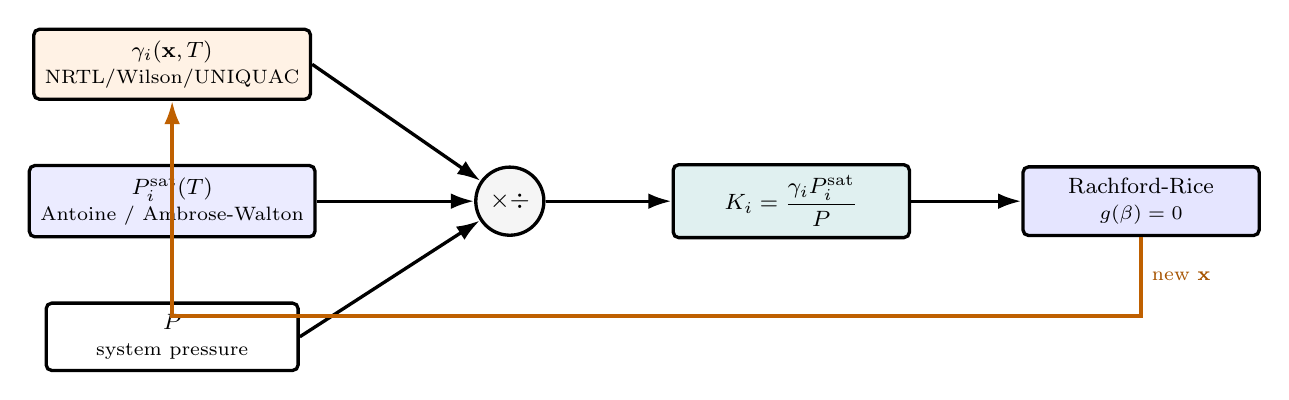
\begin{tikzpicture}[
    >={Latex[width=2.0mm]},
    src/.style ={draw, rounded corners=2pt, very thick, align=center,
                 inner sep=4pt, minimum width=32mm, font=\footnotesize},
    op/.style  ={draw, circle, very thick, minimum size=8mm, font=\small,
                 fill=gray!8},
    outx/.style ={draw, rounded corners=2pt, very thick, align=center,
                 inner sep=4pt, minimum width=30mm, font=\footnotesize,
                 fill=teal!12},
    flow/.style={->, very thick},
]
\node[src, fill=orange!10] (gam)  {$\gamma_i(\xv,T)$\\{\scriptsize NRTL/Wilson/UNIQUAC}};
\node[src, fill=blue!8, below=8mm of gam] (psat) {$P_i^{\mathrm{sat}}(T)$\\{\scriptsize Antoine / Ambrose-Walton}};
\node[src, below=8mm of psat] (pres) {$P$\\{\scriptsize system pressure}};
\node[op, right=20mm of psat] (mul) {$\times\div$};
\node[outx, right=16mm of mul] (k) {$K_i=\dfrac{\gamma_iP_i^{\mathrm{sat}}}{P}$};
\node[outx, right=14mm of k, fill=blue!10] (rr) {Rachford-Rice\\{\scriptsize $g(\beta)=0$}};
\draw[flow] (gam.east)  -- (mul);
\draw[flow] (psat.east) -- (mul);
\draw[flow] (pres.east) -- (mul);
\draw[flow] (mul) -- (k);
\draw[flow] (k)  -- (rr);
% outer-loop feedback: new x updates gamma
\draw[flow, orange!75!black] (rr.south) -- ++(0,-1.0)
   node[midway, right, font=\scriptsize, text=orange!65!black]{new $\xv$}
   -| (gam.south);
\end{tikzpicture}
\caption{What the $K$-value is, and where it sits in the flash loop.
Modified Raoult's law assembles each $K_i=\gamma_iP_i^{\mathrm{sat}}/P$
from three glass-box ingredients: the activity coefficient (from the
chosen $\Gex$ model), the pure-component vapour pressure (Antoine), and
the system pressure.  Once $\Kv$ is fixed, the flash is a \emph{pure
mass-balance} problem --- Rachford-Rice for $\beta$.  But $\gamma_i$
depends on the liquid composition $\xv$, which Rachford-Rice updates, so
the orange arrow closes an \emph{outer} loop: re-evaluate $\Kv$ at the new
$\xv$ and repeat.  This composition--$K$ coupling is exactly why the flash
needs two solver layers, not one.}
\label{fig:kvalue-assembly}
\end{figure}


The $K$-value of component $i$ is the partition ratio between vapour
and liquid:
\begin{equation}
   K_i \;\equiv\; \frac{y_i}{x_i}.
   \label{eq:K-def}
\end{equation}
Combining with \eqref{eq:modified-raoult}:
\begin{equation}
   \boxed{\;
   K_i \;=\; \frac{\gamma_i(\xv, T) \, \Psat_i(T)}{P}
   \;}
   \label{eq:K-modified-raoult}
\end{equation}
At each outer iteration, $K_i$ is a function of $T, P, \xv$ alone ---
once $\Kv$ is fixed, the flash becomes a pure mass-balance problem.

\subsection{Material balance and Rachford-Rice}

A single-stage flash takes feed $\zv$ at $F$ and splits it into
vapour $V$ at composition $\yv$ and liquid $L$ at composition $\xv$.
The component balance is:
\begin{equation}
   F z_i \;=\; V y_i + L x_i \;=\; F[\beta y_i + (1-\beta) x_i].
\end{equation}
Cancelling $F$ and using $y_i = K_i x_i$:
\[
   z_i = \beta K_i x_i + (1-\beta) x_i = x_i\,[1 + \beta(K_i - 1)],
\]
so
\begin{equation}
   x_i \;=\; \frac{z_i}{1 + \beta(K_i - 1)},
   \qquad
   y_i \;=\; \frac{K_i z_i}{1 + \beta(K_i - 1)}.
   \label{eq:xy-from-K}
\end{equation}
Imposing $\sum_i y_i - \sum_i x_i = 0$ (the closure) and collecting
terms yields the \emph{Rachford-Rice equation}:
\begin{equation}
   \boxed{\;
   g(\beta) \;\equiv\; \sum_{i=1}^{N_c} \frac{z_i \, (K_i - 1)}{1 + \beta(K_i - 1)} \;=\; 0
   \;}
   \label{eq:RR}
\end{equation}

\subsection{Why exactly one root, in $(0, 1)$, when there is two-phase}

\begin{figure}[ht]\centering
\begin{tikzpicture}
\begin{axis}[
    width=0.74\linewidth, height=5.6cm,
    xlabel={vapour fraction $\beta$},
    ylabel={$g(\beta)$},
    xmin=-0.15, xmax=1.15, ymin=-1.5, ymax=1.8,
    xtick={0,0.5,1}, ytick={0},
    axis lines=middle, clip=false,
    every axis x label/.style={at={(axis description cs:1.02,0.46)}, anchor=west},
    every axis y label/.style={at={(axis description cs:0.5,1.03)}, anchor=south},
]
% a strictly decreasing g(beta): sum z_i(K_i-1)/(1+beta(K_i-1)), 2 comps K=2.2,0.45
\addplot[domain=-0.12:1.12, samples=120, blue!70!black, very thick]
  ({x}, { 0.45*1.2/(1+x*1.2) + 0.55*(-0.55)/(1-x*0.55) });
% root marker
\addplot[only marks, mark=*, mark size=2.6pt, mark options={red!80!black}]
   coordinates {(0.503,0)};
\node[anchor=south west, font=\scriptsize, text=red!70!black]
   at (axis cs:0.50,0.05) {unique root $\beta^*$};
% endpoints
\addplot[only marks, mark=square*, mark size=2pt, mark options={gray!55!black}]
   coordinates {(0,0.237) (1,-0.298)};
\node[anchor=west, font=\scriptsize, text=gray!40!black] at (axis cs:0.02,0.40)
   {$g(0)>0$};
\node[anchor=east, font=\scriptsize, text=gray!40!black] at (axis cs:0.98,-0.45)
   {$g(1)<0$};
% physical window shading hint
\draw[dashed, gray!50!black] (axis cs:0,-1.5) -- (axis cs:0,1.8);
\draw[dashed, gray!50!black] (axis cs:1,-1.5) -- (axis cs:1,1.8);
\end{axis}
\end{tikzpicture}
\caption{Why Rachford-Rice is numerically tame.  When a two-phase region
exists, some $K_i>1$ (volatiles) and some $K_i<1$ (heavies), so
$g(0)>0$ and $g(1)<0$ --- the function changes sign across the physical
window $[0,1]$.  And $g'(\beta)<0$ everywhere it is defined (each term in
the derivative is a negative square), so $g$ is \emph{strictly
decreasing}.  A monotone function with one sign change has exactly one
root, and Newton-Raphson from any interior $\beta_0$ converges to it
quadratically.  If the flash will not converge, the bug is upstream ---
a bad $K_i$ (Antoine out of range, $\gamma_i$ blowing up), never
Rachford-Rice itself.}
\label{fig:rachford-rice-root-d1}
\end{figure}


Two properties make Rachford-Rice numerically pleasant:

\begin{figure}[ht]
\centering
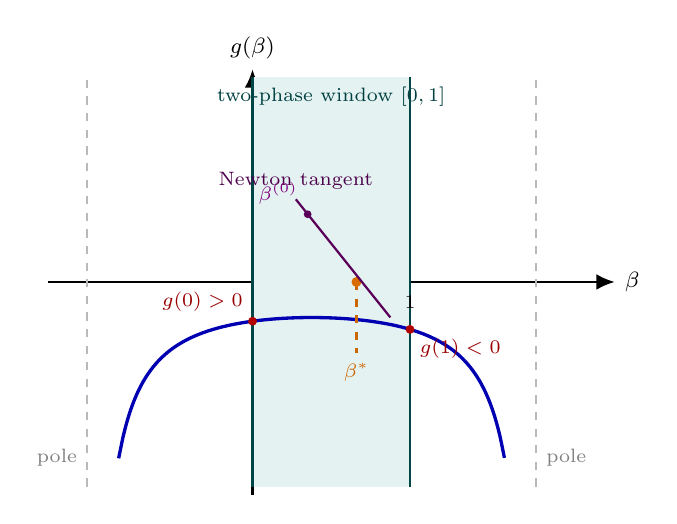
\begin{tikzpicture}[
    >={Latex[width=2.0mm]},
    every node/.style={font=\footnotesize},
    pole/.style={gray!55, dashed, thick},
]
% axes
\draw[->, thick] (-2.6,0) -- (4.6,0) node[right]{$\beta$};
\draw[->, thick] (0,-2.7) -- (0,2.7) node[above]{$g(\beta)$};
% the physical window [0,1]
\fill[teal!10] (0,-2.6) rectangle (2,2.6);
\node[teal!50!black, font=\scriptsize] at (1.0,2.35) {two-phase window $[0,1]$};
\draw[teal!55!black, thick] (0,-2.6) -- (0,2.6);
\draw[teal!55!black, thick] (2,-2.6) -- (2,2.6);
\node[font=\scriptsize, anchor=north] at (2,-0.05) {$1$};
% asymptote poles (where 1+beta(K_i-1)=0): one on each side, outside window
\draw[pole] (-2.1,-2.6) -- (-2.1,2.6)
      node[pos=0.07, left, font=\scriptsize, gray]{pole};
\draw[pole] ( 3.6,-2.6) -- ( 3.6,2.6)
      node[pos=0.07, right, font=\scriptsize, gray]{pole};
% the monotone-decreasing branch through the window (a smooth curve)
\draw[very thick, blue!70!black]
      plot[smooth, domain=-1.7:3.2, samples=80]
      ({\x}, {0.9/(\x-3.6) - 0.9/(\x+2.1) + 0.18});
% endpoint sign markers
\fill[red!70!black] (0,{0.9/(0-3.6) - 0.9/(0+2.1)+0.18}) circle (1.6pt)
      node[above left, font=\scriptsize, red!60!black]{$g(0)>0$};
\fill[red!70!black] (2,{0.9/(2-3.6) - 0.9/(2+2.1)+0.18}) circle (1.6pt)
      node[below right, font=\scriptsize, red!60!black]{$g(1)<0$};
% the root
\draw[orange!80!black, thick, dashed]
      (1.32,0) -- (1.32,-0.9) node[below, font=\scriptsize]{$\beta^\ast$};
\fill[orange!85!black] (1.32,0) circle (1.8pt);
% Newton tangent hint
\draw[violet!70!black, thick] (0.55,1.05) -- (1.75,-0.45)
      node[pos=0.0, above, font=\scriptsize, violet!60!black]{Newton tangent};
\fill[violet!70!black] (0.7,0.86) circle (1.4pt)
      node[above left, font=\scriptsize, violet]{$\beta^{(0)}$};
\end{tikzpicture}
\caption{Why Rachford--Rice is tame.  Each term has a pole where
$1+\beta(K_i{-}1)=0$; for a genuine two-phase mixture all the poles lie
\emph{outside} the physical window $[0,1]$ (shaded), so on that window
$g$ is a single, smooth, strictly \emph{decreasing} branch
($g'(\beta)<0$ always).  When a split exists the endpoints straddle zero
--- $g(0)>0$, $g(1)<0$ --- guaranteeing exactly one root $\beta^\ast$ in
$(0,1)$.  Monotone plus a sign change is the textbook recipe for a
trouble-free Newton: the tangent from \emph{any} interior $\beta^{(0)}$
slides to $\beta^\ast$ and converges quadratically.  If the endpoints
share a sign, the root is pushed outside $[0,1]$ --- the subcooled /
superheated case the flash reports honestly.}
\label{fig:rachford-rice-root}
\end{figure}


\textbf{Monotonicity.} Differentiating \eqref{eq:RR}:
\[
   g'(\beta) \;=\; -\sum_i \frac{z_i \, (K_i - 1)^2}{[1 + \beta(K_i - 1)]^2}
                 \;<\; 0.
\]
Since each term in the sum is non-negative, $g'(\beta) < 0$ wherever the
sum is defined --- $g$ is strictly decreasing.

\textbf{Sign change.} If a two-phase region exists, some $K_i > 1$ (the
volatile components) and some $K_i < 1$ (the heavy ones). Then
$g(0) = \sum_i z_i (K_i - 1)$ has the sign of "are most components
volatile?", and $g(1) = \sum_i z_i (1 - 1/K_i)$ has the opposite sign.
Both endpoints differ in sign, so a root exists in $(0, 1)$.

The combination of monotonicity and a sign change in $(0,1)$ means
Newton-Raphson starting from \emph{any} interior $\beta_0$ will converge,
quadratically, to the unique root.

\begin{keyidea}
Rachford-Rice is convex enough to make Newton-Raphson tame. If your
flash refuses to converge, the bug is upstream --- almost always a bad
$K_i$ (Antoine outside its range; $\gamma_i$ blowing up; $T$ below
the lower phase boundary).
\end{keyidea}

\subsection{Initialisation: the Wilson $K$-value}

A robust initial guess for $\Kv$ before any activity-coefficient
information is available comes from Wilson's correlation:
\begin{equation}
   K_i^{(0)}(T, P) \;=\; \frac{P_{c,i}}{P}\,
                         \exp\!\Bigl[\,5.373\,(1 + \omega_i)\,
                         \bigl(1 - T_{c,i}/T\bigr)\Bigr].
   \label{eq:wilson-K}
\end{equation}
This uses only the critical point and the acentric factor --- both in
the component database --- and works astonishingly well as a starting
point.

\subsection{Worked example}

\begin{example}[Flash of benzene/toluene at 370\,K, 1\,bar]
A feed at $\zv = (0.40,\, 0.60)$ (benzene then toluene), $T = 370\,K$,


$P = 1\,$bar.  At this temperature, Antoine gives
$\Psat_1 \approx 1.46\,$bar and $\Psat_2 \approx 0.61\,$bar. Ideal
solution: $\gamma_i = 1$, so $K_1 = 1.46$ and $K_2 = 0.61$.

Rachford-Rice:
\[
   g(\beta) \;=\; \frac{0.40 \cdot 0.46}{1 + 0.46 \beta} \,+\,
                  \frac{0.60 \cdot (-0.39)}{1 - 0.39 \beta} \;=\; 0.
\]
At $\beta = 0$: $g = 0.184 - 0.234 = -0.050$. At $\beta = 1$:
$g = 0.126 - 0.383 = -0.257$. Both endpoints are negative --- so this
feed is below the bubble point. Iterating Newton on $g$ starting from
$\beta_0 = -0.1$ converges quickly to $\beta \approx -0.13$, which is
unphysical: confirmation that the mixture is sub-cooled at $370\,K$. To
get a two-phase split we need $T \gtrsim 375\,$K. This is exactly the
\code{flash01\_benzene\_toluene} setup; the simulator will report the
unphysical $\beta$ and warn.
\end{example}

\begin{figure}[ht]\centering
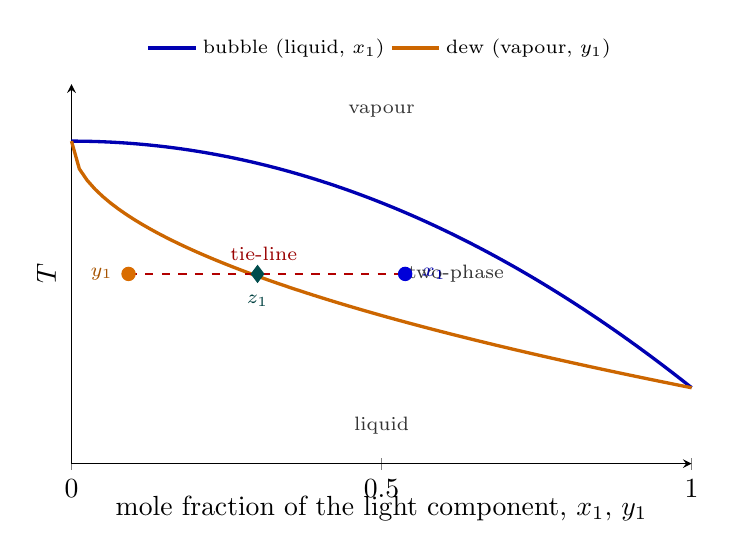
\begin{tikzpicture}
\begin{axis}[
    width=0.78\linewidth, height=6.4cm,
    xlabel={mole fraction of the light component, $x_1,\,y_1$},
    ylabel={$T$},
    xmin=0, xmax=1, ymin=0, ymax=1,
    xtick={0,0.5,1}, ytick=\empty,
    axis lines=left, clip=false,
    legend style={font=\scriptsize, at={(0.5,1.04)}, anchor=south, draw=none},
    legend columns=2,
    every axis x label/.style={at={(axis description cs:0.5,-0.06)}, anchor=north},
]
% bubble (lower, in x) and dew (upper, in y) curves, both from T at x=1 (low) to x=0 (high)
\addplot[domain=0:1, samples=80, blue!70!black, very thick]
   ({x}, {0.85 - 0.65*x*x});            % bubble: T vs x1
\addlegendentry{bubble (liquid, $x_1$)}
\addplot[domain=0:1, samples=80, orange!80!black, very thick]
   ({x}, {0.85 - 0.65*sqrt(x)});        % dew: T vs y1
\addlegendentry{dew (vapour, $y_1$)}
% region labels
\node[font=\scriptsize, text=gray!40!black] at (axis cs:0.5,0.93) {vapour};
\node[font=\scriptsize, text=gray!40!black] at (axis cs:0.5,0.10) {liquid};
\node[font=\scriptsize, text=gray!40!black] at (axis cs:0.62,0.5) {two-phase};
% a tie line at T = 0.5
\draw[dashed, red!70!black, thick] (axis cs:0.092,0.5) -- (axis cs:0.538,0.5);
\addplot[only marks, mark=*, mark size=2.4pt, mark options={blue!85!black}]
   coordinates {(0.538,0.5)};
\addplot[only marks, mark=*, mark size=2.4pt, mark options={orange!85!black}]
   coordinates {(0.092,0.5)};
\node[anchor=west, font=\scriptsize, text=blue!65!black]  at (axis cs:0.55,0.5) {$x_1$};
\node[anchor=east, font=\scriptsize, text=orange!65!black] at (axis cs:0.082,0.5) {$y_1$};
\node[anchor=south, font=\scriptsize, text=red!60!black] at (axis cs:0.31,0.51) {tie-line};
% feed composition vertical
\addplot[only marks, mark=diamond*, mark size=3pt, mark options={teal!60!black}]
   coordinates {(0.30,0.5)};
\node[anchor=north, font=\scriptsize, text=teal!50!black] at (axis cs:0.30,0.47) {$z_1$};
\end{axis}
\end{tikzpicture}
\caption{A temperature--composition ($Txy$) diagram, the phase-diagram
face of the flash.  The lower (blue) curve is the bubble locus, plotted
against the \emph{liquid} composition $x_1$; the upper (orange) curve is
the dew locus, plotted against the \emph{vapour} composition $y_1$.
Between them lies the two-phase region.  At a flash temperature, the
horizontal \emph{tie-line} (red) connects the coexisting liquid $x_1$ and
vapour $y_1$ in equilibrium ($y_1=K_1x_1$).  A feed of composition $z_1$
(diamond) lands inside the lens, and the lever rule along the tie-line
fixes the vapour fraction $\beta$ that Rachford-Rice computes.  Outside
the lens there is a single phase --- below it sub-cooled liquid, above it
superheated vapour.}
\label{fig:txy-tielines}
\end{figure}

\begin{tutoriallink}
\file{tutorials/flash01\_benzene\_toluene} --- run with
\code{verbosity 3} and watch the Newton trace converge in 3--4
iterations.
\end{tutoriallink}

\section*{Part IV --- Numerical methods}
\phantomsection
\addcontentsline{toc}{section}{Part IV --- Numerical methods}

\stepcounter{thpart}
\setcounter{section}{0}

% ---------------------------------------------------------------------
\section{Numerical methods, gently}\label{ch:gentle}

\begin{whatyoulllearn}
A first look at root-finding, with no Jacobians and no Taylor
expansions yet.  We will pose one concrete chemical-engineering
problem --- the bubble temperature of a benzene/toluene mixture ---
and solve it four times: by hand, by bisection, by secant, and
finally by Newton-Raphson.  By the end you will have a feel for
\emph{why} the simulator uses Newton everywhere instead of just
guessing, and the heavier chapters that follow (Newton-1D, Newton in
$n$ dimensions, Levenberg-Marquardt) will read as natural
generalisations of what you just did by hand.
\end{whatyoulllearn}

\subsection{One problem, four strategies}

Mix 50~mol\% benzene and 50~mol\% toluene in a sealed vessel at
\textbf{$P = 1$~bar} and slowly heat the liquid.  At what temperature
does the first vapour bubble form?

For an ideal Raoult mixture the bubble condition is
\begin{equation}
   x_b\, P^{\mathrm{sat}}_b(T) \;+\; x_t\, P^{\mathrm{sat}}_t(T) \;=\; P,
   \label{eq:gentle-bubble}
\end{equation}
which with $x_b = x_t = 0.5$ and $P = 1$~bar reduces to
$P^{\mathrm{sat}}_b(T) + P^{\mathrm{sat}}_t(T) = 2$~bar.  Both saturation
pressures come from Antoine,
\[
   \log_{10} P^{\mathrm{sat}}(T) \;=\; A \;-\; \frac{B}{T+C},
\]
with the constants shipped in
\file{data/standards/components/}: $A_b = 4.0181$, $B_b = 1203.84$,
$C_b = -53.23$~K for benzene; $A_t = 4.0783$, $B_t = 1343.94$,
$C_t = -53.77$~K for toluene.

Define the \textbf{residual}
\begin{equation}
   f(T) \;\equiv\; \tfrac{1}{2}\bigl[P^{\mathrm{sat}}_b(T) + P^{\mathrm{sat}}_t(T)\bigr] - 1,
\end{equation}
which is zero exactly at the bubble temperature.  Knowing $T_b
\approx 353$~K and $T_t \approx 384$~K, the answer must lie somewhere
between those, but where?

\begin{intuition}
Every numerical method in this book solves the same shape of problem:
\textbf{given a function $f$, find a $T$ for which $f(T) = 0$}.  The
strategies differ only in how cleverly they use the available
information about $f$.  The dumbest method needs only the ability to
evaluate $f$; the smartest also needs $f'$.  More information you
exploit, fewer evaluations you need.
\end{intuition}

\subsection{Strategy 1 --- guess and adjust}

Pick a temperature, compute $f$, see whether it is positive or
negative, adjust.  Honest, slow, but absolutely transparent:

\begin{center}
\small
\begin{tabular}{cc}
\toprule
$T$ [K] & $f(T)$ [bar]\\
\midrule
340 & $-0.55$ \\
360 & $-0.13$ \\
380 & $+0.53$ \\
365 & $+0.0053$ \\
364 & $-0.024$ \\
\bottomrule
\end{tabular}
\end{center}

After five tries we know the root is between 364 and 365~K and
closer to the upper bound.  Two more refinements get us to within
$0.05$~K of the answer.  The procedure works but you do all the
thinking.

\subsection{Strategy 2 --- bisection}

Trial-and-error implicitly used a fundamental fact: $f$ is
continuous, $f(340) < 0$, $f(390) > 0$, so by the intermediate
value theorem the root sits somewhere in $[340, 390]$.  Bisection
mechanises that intuition: take the midpoint, evaluate $f$, keep
the half that still brackets the root.

\begin{example}[Bisection on Eq.~\eqref{eq:gentle-bubble}]
Starting bracket $[340, 390]$.  Midpoint $T_1 = 365$, $f(T_1) = +0.0053$.
Since $f$ changed sign on the lower half, replace $b$ with $T_1$ and
repeat:
\begin{center}\small
\begin{tabular}{rrr}
\toprule
iter & $T$ [K] & $f$ [bar]\\
\midrule
 1 & 365.000 & $+5.34\times 10^{-3}$\\
 2 & 352.500 & $-3.15\times 10^{-1}$\\
 3 & 358.750 & $-1.67\times 10^{-1}$\\
 5 & 363.438 & $-4.02\times 10^{-2}$\\
 8 & 364.805 & $-4.43\times 10^{-4}$\\
12 & 364.817 & $-8.24\times 10^{-5}$\\
20 & 364.820 & $\pm 7\times 10^{-7}$\\
\bottomrule
\end{tabular}
\end{center}
After 20 iterations $T \approx 364.820$~K.
\end{example}

Bisection is a tortoise: every iteration halves the bracket, so the
error decays exactly by a factor 2.  To get from a 50~K wide bracket
down to a $10^{-7}$~K tolerance takes roughly $\log_2(50/10^{-7})
\approx 29$ steps.  Never blows up, never overshoots --- but never
fast either.

\subsection{Strategy 3 --- secant}

Bisection only uses the \emph{sign} of $f$ at each midpoint.  We can
do better by exploiting the \emph{value}: if $f$ has changed by a
known amount between two trial $T$'s, a linear extrapolation
predicts where it would hit zero.  Geometrically, draw the secant
line through the last two points and read off the $T$-intercept:
\begin{equation}
   T_{k+1} \;=\; T_k \;-\; f(T_k)\,\frac{T_k - T_{k-1}}{f(T_k) - f(T_{k-1})}.
   \label{eq:secant}
\end{equation}

\begin{example}[Secant on Eq.~\eqref{eq:gentle-bubble}]
Starting from the same two points $(T_0, T_1) = (340, 390)$~K:
\begin{center}\small
\begin{tabular}{rrr}
\toprule
iter & $T$ [K] & $f$ [bar]\\
\midrule
1 & 357.817 & $-1.91\times 10^{-1}$\\
2 & 363.009 & $-5.24\times 10^{-2}$\\
3 & 364.975 & $+4.60\times 10^{-3}$\\
4 & 364.816 & $-9.74\times 10^{-5}$\\
5 & 364.81968 & $-1.76\times 10^{-7}$\\
6 & 364.81969 & $+6.7\times 10^{-12}$\\
\bottomrule
\end{tabular}
\end{center}
Six iterations to machine precision.
\end{example}

Each step uses two function evaluations of history, no derivatives.
The order of convergence is $\varphi = (1 + \sqrt{5})/2 \approx
1.618$ --- the golden ratio.  In practice this means the number of
correct digits multiplies by 1.6 each iteration: 1 digit, 2, 3, 5,
8, 12 --- so it doubles roughly every two iterations.

\begin{pitfall}
The secant formula breaks if $f(T_k) = f(T_{k-1})$ (division by
zero).  Bisection cannot break that way.  In practice the simulator
falls back to bisection whenever the secant step would carry the
iterate outside the current bracket.
\end{pitfall}

\subsection{Strategy 4 --- Newton-Raphson, in one breath}

Secant approximated the slope of $f$ from two adjacent evaluations.
What if we knew the slope exactly --- the derivative $f'(T)$?  Then
we could shoot a line off the current point and intersect zero in
\emph{one} step:
\begin{equation}
   \boxed{\;
   T_{k+1} \;=\; T_k \;-\; \frac{f(T_k)}{f'(T_k)}.
   \;}
\end{equation}
That is Newton-Raphson.  The next chapter derives it rigorously
from a Taylor expansion; here we just apply it.

\begin{example}[Newton on Eq.~\eqref{eq:gentle-bubble}]
Start from $T_0 = 340$~K with $f'(T)$ computed numerically (or, more
typically in this simulator, analytically from $\mathrm{d}P^{\mathrm{sat}}/\mathrm{d}T$):
\begin{center}\small
\begin{tabular}{rrr}
\toprule
iter & $T$ [K] & $f$ [bar]\\
\midrule
1 & 374.942 & $+3.36\times 10^{-1}$\\
2 & 365.872 & $+3.15\times 10^{-2}$\\
3 & 364.832 & $+3.74\times 10^{-4}$\\
4 & 364.8197 & $+5.5\times 10^{-8}$\\
5 & 364.8197 & $+2.4\times 10^{-15}$\\
\bottomrule
\end{tabular}
\end{center}
Four iterations to $10^{-8}$, five to machine precision.
\end{example}

Look at the residual column above.  At iteration~3 it is
$3.7\times 10^{-4}$; at iteration~4 it is $5.5\times 10^{-8}$.  The
exponent jumped from $-4$ to $-8$ --- the error \textbf{squared}.
That is the signature of \textbf{quadratic convergence}, and it is
the reason every iterative solver in this simulator is Newton-based
when a derivative is available.

\begin{intuition}
``Quadratic'' here means the number of correct decimal digits
\emph{doubles} every iteration: 2 digits, 4, 8, 16, machine
precision.  Bisection adds one bit per step; secant multiplies digits
by 1.6; Newton multiplies digits by 2.  This is why even though
Newton needs the extra information $f'$, it pays back so dramatically
that it is essentially never not worth it.
\end{intuition}

\subsection{The four strategies side by side}

Figure~\ref{fig:gentle-convergence} plots $|f(T_k)|$ versus iteration
number for the four runs on a semi-log axis.  The slope of each line
is the convergence rate.

\begin{figure}[h]
\centering
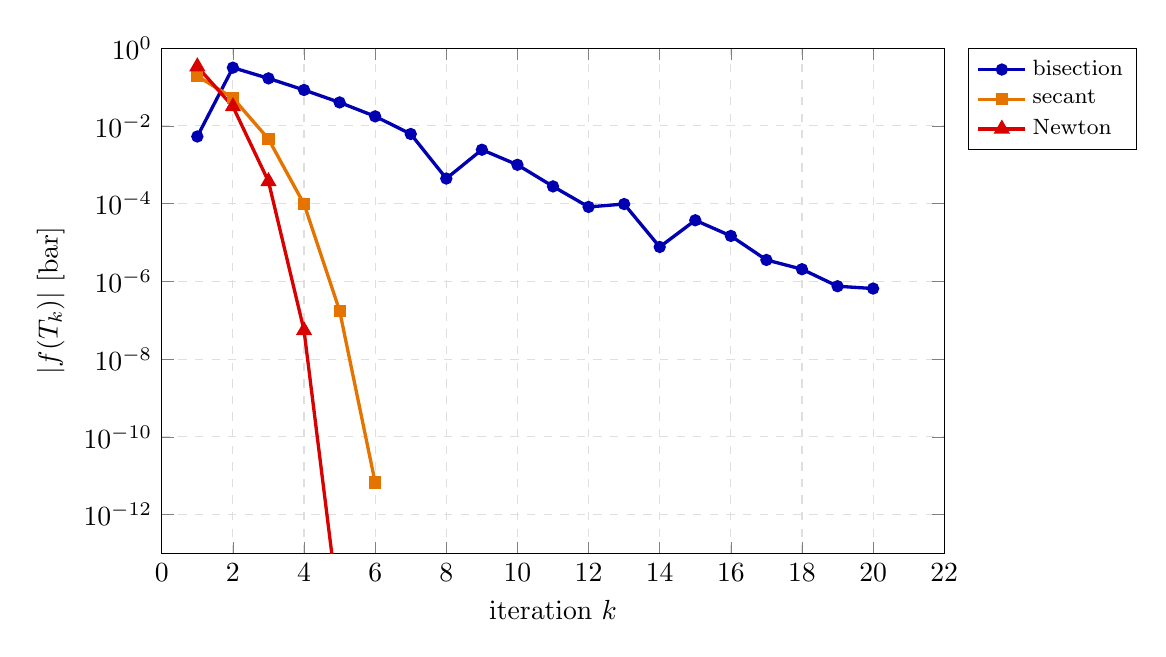
\begin{tikzpicture}
\begin{semilogyaxis}[
    width=0.95\linewidth, height=8cm,
    xlabel={iteration $k$},
    ylabel={$|f(T_k)|$ [bar]},
    xmin=0, xmax=22,
    ymin=1e-13, ymax=1,
    grid=major,
    grid style={gray!25, dashed},
    legend pos=outer north east,
    legend cell align=left,
    legend style={font=\footnotesize},
]
% Bisection (linear, slope ~ log10(2) per step)
\addplot[blue!70!black, very thick, mark=*, mark size=1.6pt] coordinates {
    (1, 5.34e-3) (2, 3.15e-1) (3, 1.67e-1) (4, 8.40e-2)
    (5, 4.02e-2) (6, 1.76e-2) (7, 6.20e-3) (8, 4.43e-4)
    (9, 2.44e-3) (10, 9.99e-4) (11, 2.78e-4) (12, 8.24e-5)
    (13, 9.78e-5) (14, 7.70e-6) (15, 3.74e-5) (16, 1.48e-5)
    (17, 3.57e-6) (18, 2.06e-6) (19, 7.52e-7) (20, 6.56e-7)
};
\addlegendentry{bisection}
% Secant (superlinear, golden-ratio order)
\addplot[orange!90!black, very thick, mark=square*, mark size=1.6pt] coordinates {
    (1, 1.91e-1) (2, 5.24e-2) (3, 4.60e-3) (4, 9.74e-5)
    (5, 1.76e-7) (6, 6.7e-12)
};
\addlegendentry{secant}
% Newton (quadratic)
\addplot[red!85!black, very thick, mark=triangle*, mark size=2.2pt] coordinates {
    (1, 3.36e-1) (2, 3.15e-2) (3, 3.74e-4) (4, 5.5e-8) (5, 2.4e-15)
};
\addlegendentry{Newton}
\end{semilogyaxis}
\end{tikzpicture}
\caption{Residual decay for the four strategies on the same
benzene/toluene bubble-temperature problem (initial bracket
$[340, 390]$~K, target $T_b \approx 364.82$~K).  Bisection is
straight on the semi-log plot --- a constant factor of $\sim 2$ per
step.  Secant accelerates with the slope steepening over time.
Newton dives off the chart in five steps.}
\label{fig:gentle-convergence}
\end{figure}

\begin{center}
\small
\begin{tabular}{lcccc}
\toprule
method & uses        & per-iter cost & order $p$ & iters to $10^{-8}$\\
\midrule
trial \& error & $f$ values + intuition & 1 eval & --- & many \\
bisection      & $f$ signs              & 1 eval & 1 (linear) & $\sim$30 \\
secant         & last 2 $f$ values      & 1 eval & 1.618 & $\sim$6 \\
Newton         & $f$ \emph{and} $f'$    & 1 eval $+$ 1 deriv & 2 (quadratic) & $\sim$4 \\
\bottomrule
\end{tabular}
\end{center}

\subsection{Why the rest of Part III matters}

Every solver in the simulator is a generalisation of these four

\begin{figure}[ht]
\centering
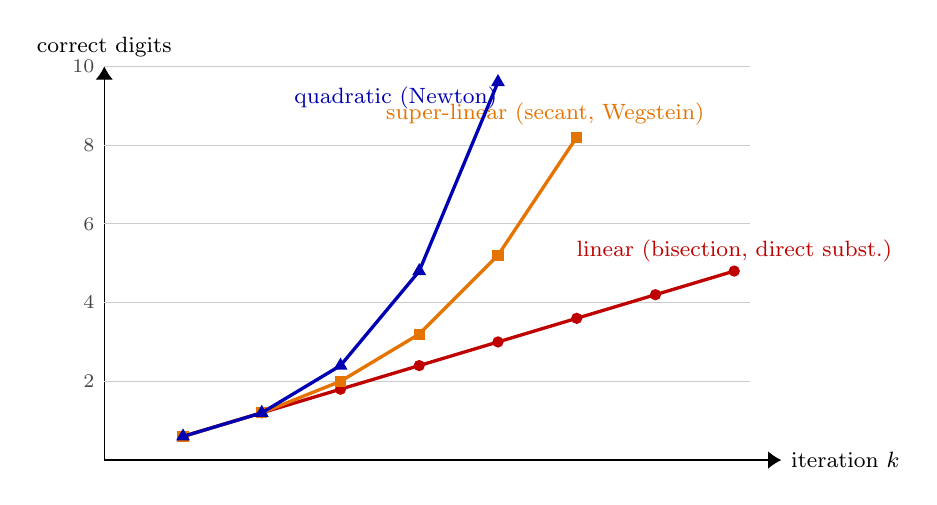
\begin{tikzpicture}[
    >={Latex[width=2.2mm]},
    every node/.style={font=\footnotesize},
    scale=1.0,
]
% three rungs showing how many correct digits per step each order buys.
\draw[->] (0,0) -- (8.6,0) node[right] {iteration $k$};
\draw[->] (0,0) -- (0,5.0) node[above] {correct digits};
\foreach \y/\d in {1/2,2/4,3/6,4/8,5/10}{\draw[gray!40] (0,\y) -- (8.2,\y); \node[left,gray!55!black,font=\scriptsize] at (0,\y) {\d};}
% linear: +constant digits per step -> red
\draw[red!75!black, very thick, mark=*, mark size=1.4pt]
   plot coordinates {(1,0.3)(2,0.6)(3,0.9)(4,1.2)(5,1.5)(6,1.8)(7,2.1)(8,2.4)};
\node[red!75!black] at (8.0,2.65) {linear (bisection, direct subst.)};
% super-linear: digits *1.6 growth -> orange
\draw[orange!90!black, very thick, mark=square*, mark size=1.4pt]
   plot coordinates {(1,0.3)(2,0.6)(3,1.0)(4,1.6)(5,2.6)(6,4.1)};
\node[orange!90!black] at (5.6,4.4) {super-linear (secant, Wegstein)};
% quadratic: digits double -> blue
\draw[blue!70!black, very thick, mark=triangle*, mark size=1.7pt]
   plot coordinates {(1,0.3)(2,0.6)(3,1.2)(4,2.4)(5,4.8)};
\node[blue!70!black] at (3.7,4.6) {quadratic (Newton)};
\end{tikzpicture}
\caption{The three convergence \emph{orders} that organise every solver
in this manual, read as ``how many correct digits each step buys.''
\emph{Linear} convergence (red --- bisection, direct substitution) adds a
roughly constant number of digits per step, so the digit count climbs
along a straight line.  \emph{Super-linear} (orange --- the secant and
Wegstein) speeds up as it goes: the per-step gain itself grows.
\emph{Quadratic} (blue --- Newton and its $n$-D and tear-loop
descendants) \emph{doubles} the correct digits every step once it is
near the root, which is why Newton clears twelve digits in a handful of
iterations.  Damping and finite-difference Jacobians are the price paid
to keep a method on its fast curve without falling off into divergence
far from the root.}
\label{fig:convergence-orders}
\end{figure}

moves:
\begin{itemize}[leftmargin=*,nosep]
  \item Chapter~\ref{ch:nr1d} re-derives Newton from Taylor's
        theorem, formalises ``convergence,'' and shows how the
        simulator damps an overshoot or falls back to bisection
        when the local linear model misleads.
  \item The next chapter generalises Newton to vector equations
        --- the kind that pop up the moment you have multiple
        unknowns (multi-component flash, adiabatic flash, rigorous
        distillation).  Replace ``$f'(T_k)$'' by a \emph{Jacobian
        matrix}; replace ``divide'' by ``solve a linear system.''
        Nothing else changes.
  \item Levenberg-Marquardt is Newton plus a damping knob that
        lets it gracefully degrade to gradient descent when the
        linear model is bad.  We use it for parameter estimation
        from experimental data.
  \item Wegstein and direct substitution attack a different shape
        of problem ($x = f(x)$ rather than $f(x) = 0$) and
        accelerate fixed-point iterations.  We use them on
        activity-coefficient outer loops where computing a
        derivative is awkward.
\end{itemize}

Keep the four strategies in mind as you read on.  Every more elaborate
algorithm in this manual is, at heart, one of them dressed up.

% ---------------------------------------------------------------------
\section{Newton-Raphson, one dimension}\label{ch:nr1d}

\begin{whatyoulllearn}
The single algorithm that solves every scalar fixed-point in the
simulator. Why it converges quadratically when it converges, and what
damping is for.
\end{whatyoulllearn}

\subsection{Derivation}

Given a continuously differentiable $g \colon \R \to \R$ and a root
$x^*$ with $g(x^*) = 0$, Taylor-expand around an estimate $x_k$:
\[
   0 \;=\; g(x^*) \;=\; g(x_k) + g'(x_k)\,(x^* - x_k) + O((x^* - x_k)^2).
\]
Solving for $x^*$ and dropping the higher-order term defines the
\emph{Newton iteration}:
\begin{equation}
   \boxed{\;
   x_{k+1} \;=\; x_k \;-\; \frac{g(x_k)}{g'(x_k)}
   \;}
   \label{eq:newton-1d}
\end{equation}

% --- Figure: Newton tangent (geometric construction) ------------------
\begin{figure}[h]
\centering
\begin{tikzpicture}[
    >={Latex[width=2.5mm]},
    every node/.style={font=\footnotesize},
    scale=2.0,
]
% Axes
\draw[->] (0.4, 0) -- (2.7, 0) node[right] {$x$};
\draw[->] (0.5, -1.5) -- (0.5, 3.0) node[above] {$g(x)$};
\node[below left] at (0.5, 0) {$0$};

% Curve g(x) = x^2 - 2  (sampled)
\draw[blue, very thick, smooth] plot[domain=0.5:2.55, samples=40] (\x, {\x*\x - 2})
    node[right, text=blue] {$g(x)$};

% Tick at x_k = 2 (on x-axis)
\filldraw[blue!70!black] (2, 2) circle (0.6pt);
\draw[dashed, blue!50!black] (2, 0) -- (2, 2);
\node[below] at (2, -0.05) {$x_k$};
\node[left=2pt, blue!70!black] at (2, 2) {$\bigl(x_k, g(x_k)\bigr)$};

% Tangent line at (2, 2) with slope g'(2) = 4: y = 4(x-2) + 2 = 4x - 6
% Domain: x_{k+1} = 1.5 (where tangent crosses y=0), extend a bit
\draw[red, very thick] (1.35, -0.6) -- (2.25, 3.0);
\node[right, text=red] at (2.25, 3.0) {tangent, slope $g'(x_k)$};

% x_{k+1} = 1.5
\filldraw[red] (1.5, 0) circle (0.6pt);
\node[below] at (1.5, -0.05) {$x_{k+1}$};

% Root x* = sqrt(2) ≈ 1.414
\filldraw[gray!50!black] (1.4142, 0) circle (0.6pt);
\node[below, gray!50!black] at (1.4142, -0.18) {$x^*$};
\node[above left, font=\scriptsize, text=gray!50!black] at (1.4142, 0) {$\sqrt{2}$};

% Subtle arrow from x_k to x_{k+1} to show iteration
\draw[->, gray!50!black, thin, dashed]
    (2, -0.32) to[bend left=10] node[midway, below=1pt, font=\scriptsize, text=gray!50!black]
    {one Newton step} (1.5, -0.32);

\end{tikzpicture}
\caption{One Newton iteration on $g(x) = x^2 - 2$ (root $x^* =
\sqrt{2} \approx 1.4142$).  At the current estimate $x_k = 2$, draw the
tangent to $g$ at $(x_k, g(x_k))$ with slope $g'(x_k) = 4$; the
tangent's $x$-intercept is the next estimate $x_{k+1} = 1.5$.  Two
more iterations from there converge to $x^*$ to twelve digits ---
the quadratic doubling of correct digits per step that gives Newton
its reputation.}
\label{fig:newton-1d-tangent}
\end{figure}

\subsection{Convergence}

Define the error $e_k \equiv x_k - x^*$. A second-order Taylor expansion
of $g$ around $x^*$ gives
\[
   g(x_k) \;=\; g'(x^*)\,e_k \;+\; \tfrac{1}{2} g''(x^*)\,e_k^2 \;+\; O(e_k^3),
\]
and similarly $g'(x_k) = g'(x^*) + g''(x^*) e_k + O(e_k^2)$. Substituting
into \eqref{eq:newton-1d} and keeping leading order in $e_k$:
\begin{equation}
   e_{k+1} \;=\; \frac{g''(x^*)}{2\,g'(x^*)} \, e_k^2 \;+\; O(e_k^3).
\end{equation}
This is \emph{quadratic convergence}: the error squares at each step,
provided $g'(x^*) \ne 0$ and we start close enough to $x^*$.

\subsection{Damping}

Far from the root, the linearisation can over-shoot --- pushing $x_{k+1}$
into a region where $g'$ has the wrong sign, or even outside the
domain of $g$. A damping factor $\lambda \in (0, 1]$ tames this:
\begin{equation}
   x_{k+1} \;=\; x_k - \lambda \,\frac{g(x_k)}{g'(x_k)},
\end{equation}
with $\lambda$ reduced (typically halved) until
$|g(x_{k+1})| < |g(x_k)|$. This loses quadratic convergence \emph{near
the root} (where $\lambda$ returns to 1 anyway), but buys global
robustness. The simulator's \code{NewtonRaphson} uses backtracking
damping with a halving schedule.

\subsection{Worked example}

\begin{example}[Bubble pressure of benzene/toluene]
Solve $g(P) = \sum_i x_i \gamma_i \Psat_i(T) / P - 1 = 0$ for $P$ at
$T = 365\,$K, $x_1 = 0.4$ benzene, ideal solution.

At $T = 365\,$K Antoine gives $\Psat_1 \approx 1.20$ bar,
$\Psat_2 \approx 0.49$ bar. So $g(P) = (0.4 \cdot 1.20 + 0.6 \cdot 0.49)/P - 1 = 0.774/P - 1$.

This is linear in $1/P$ --- the root is $P^* = 0.774$ bar in one
``Newton step''. Real cases with $\gamma_i = \gamma_i(\xv, T)$ are
non-linear: typical convergence is 3--5 steps to $|g| < 10^{-8}$.
\end{example}

% ---------------------------------------------------------------------
\section{Newton-Raphson, \texorpdfstring{$n$}{n} dimensions}\label{ch:nrND}

\begin{whatyoulllearn}
Most non-trivial equations in a process simulator have more than one
unknown.  This chapter generalises the Newton step of \S\ref{ch:nr1d}
to a system of $n$ coupled equations in $n$ unknowns.  The key
conceptual leap is that a derivative becomes a \emph{Jacobian
matrix}, and the division $g/g'$ becomes a \emph{linear-system
solve} $\Jac\,\Delta\xv = -\Fv$.  Everything else --- damping,
finite-difference approximation, convergence behaviour --- carries
over from the scalar case once that leap is made.
\end{whatyoulllearn}

\subsection{Why we need a multi-dimensional Newton}

The 1-D Newton iteration solves one equation in one unknown.  Lots of
chemistry is not like that.  A few representative examples from this
simulator:

\begin{itemize}[leftmargin=*,nosep,topsep=2pt]
  \item \textbf{Multi-component flash.}  At fixed $(T,P,\zv)$, the
        Rachford-Rice equation determines $V/F$ \emph{given} the
        $K_i$'s; but the $K_i$'s themselves depend on the unknown
        liquid composition $\xv$, which in turn depends on $V/F$.
        If we close this loop simultaneously instead of with an outer
        Wegstein loop, we get $n_c$ coupled equations in $n_c$ unknowns.
  \item \textbf{Adiabatic flash.}  Both $T$ and $V/F$ are unknown;
        the system is two equations (component-balance closure +
        energy balance) in two unknowns.
  \item \textbf{Rigorous distillation.}  Each stage contributes its
        own MESH equations (Mass, Equilibrium, Summations,
        Heat balance); a column with $N_s$ stages and $n_c$
        components builds a system of $O(N_s n_c)$ coupled equations.
        Naphtali--Sandholm uses Newton-ND on the whole block.
  \item \textbf{Reactive distillation.}  A reaction on the catalytic
        stages adds, per reactive stage $j$, the source $\nu_i\,\xi_j$
        to that stage's component balance, with the molar extent
        $\xi_j$ set either by chemical \emph{equilibrium},
        \(
            \sum_i \nu_i \ln\!\big(\gamma_i\,x_{j,i}\big) = \ln K_a(T_j),
        \)
        (one extra unknown $\xi_j$ and one extra equation per stage), or
        by a \emph{rate} law $\xi_j = r_j\,m_{\mathrm{cat},j}$ (no extra
        unknown --- $\xi_j$ is a function of $x_j,T_j$).  Because the
        reaction makes the residual far more nonlinear, it is converged by
        \emph{homotopy}: solve the column non-reactive first, then switch
        the reaction on, seeded from that profile.  For a mole-conserving
        ($\sum_i\nu_i=0$) reaction the constant-molal-overflow flow
        profile is undisturbed; the worked methyl-acetate case is in the
        User Guide, \S\ref{sec:advanced-distillation} of that document.
\end{itemize}
The pattern is universal: residuals $F_i$ that all depend on all the
unknowns $x_j$, and zero of them can be solved independently.

\subsection{Generalising Taylor: the Jacobian matrix}

We want to solve
\begin{equation}
   \Fv(\xv) \;=\; \mathbf{0}, \qquad \Fv \colon \R^n \to \R^n.
   \label{eq:newton-nd-system}
\end{equation}
Each $F_i$ is a function of all $n$ variables $x_1, \dots, x_n$.
Around an estimate $\xv_k$, the analog of the scalar Taylor expansion
$g(x^{\!*}) = g(x_k) + g'(x_k)(x^{\!*} - x_k) + \cdots$ is the
\emph{matrix-vector} Taylor expansion
\begin{equation}
   \mathbf{0} \;=\; \Fv(\xv^{\!*})
   \;=\; \Fv(\xv_k) + \Jac(\xv_k)\,(\xv^{\!*} - \xv_k) + O(|\xv^{\!*} - \xv_k|^2),
   \label{eq:newton-nd-taylor}
\end{equation}
where the role of $g'$ is now played by the \emph{Jacobian matrix}
$\Jac \in \R^{n\times n}$ whose entries are all the partial
derivatives,
\begin{equation}
   \Jac_{ij}(\xv_k) \;\equiv\; \left.\frac{\partial F_i}{\partial x_j}\right|_{\xv_k}.
   \label{eq:newton-nd-jacobian}
\end{equation}
Row $i$ of $\Jac$ is the gradient of $F_i$; column $j$ describes how
all $n$ residuals change when we move $x_j$ alone.

\paragraph{Geometric reading.}  The map $\xv \mapsto \Fv(\xv)$ sends
$\R^n \to \R^n$; the Jacobian $\Jac(\xv_k)$ is the \emph{best linear
approximation} of that map at $\xv_k$.  Equation
\eqref{eq:newton-nd-taylor} says that $\Fv$ is, to first order,
$\Jac \cdot \Delta\xv$ plus a constant shift.

\subsection{The Newton step in $n$ dimensions}

Dropping the higher-order term in \eqref{eq:newton-nd-taylor} and
solving for $\xv^{\!*}$ gives, formally,
$\xv^{\!*} \approx \xv_k - \Jac^{-1}\Fv(\xv_k)$.  In practice we do
\emph{not} compute $\Jac^{-1}$; we solve the linear system
\begin{equation}
   \boxed{\;
   \Jac(\xv_k)\,\Delta\xv \;=\; -\,\Fv(\xv_k),
   \qquad
   \xv_{k+1} \;=\; \xv_k + \lambda \, \Delta\xv,
   \;}
   \label{eq:newton-nd}
\end{equation}
where $\lambda \in (0,1]$ is the damping factor (next subsection).
Solving the system is both \emph{cheaper} (one LU factorisation,
$O(n^3/3)$ flops) and \emph{numerically more stable} than forming
the explicit inverse ($O(n^3)$ flops, more accumulated round-off,
hard to keep accurate when $\Jac$ is poorly conditioned).

\begin{intuition}
The scalar Newton step $x_{k+1} = x_k - g(x_k)/g'(x_k)$ asks
\emph{``how far do I have to slide $x$ to make the linear model of
$g$ hit zero?''}.  The $n$-D version asks the same question, but the
answer is a \emph{direction vector} in $\R^n$ rather than a single
scalar, and we find it by solving a linear system instead of doing a
division.  Setting $n = 1$ in \eqref{eq:newton-nd} recovers
\eqref{eq:newton-1d}: $\Jac$ becomes the scalar $g'$, and the
``linear system'' degenerates to one equation $g'(x)\Delta x = -g(x)$.
\end{intuition}

% --- Figure: the NewtonND iteration as a flowchart --------------------
\begin{figure}[h]
\centering
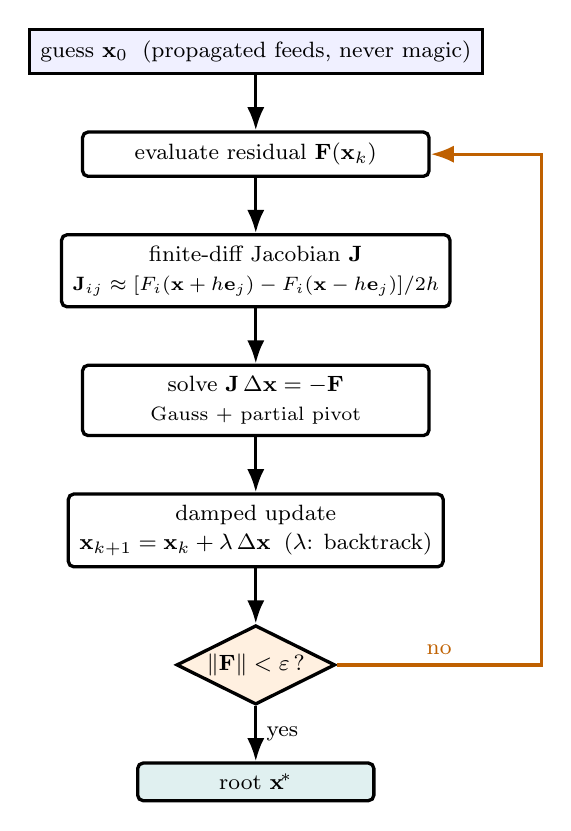
\begin{tikzpicture}[
    >={Latex[width=2.2mm]},
    node distance = 7mm and 14mm,
    every node/.style={font=\footnotesize},
    box/.style   ={draw, rounded corners=2pt, very thick,
                   align=center, inner sep=4pt, minimum width=44mm},
    io/.style    ={draw, very thick, align=center, inner sep=4pt,
                   fill=blue!6, minimum width=44mm},
    test/.style  ={draw, diamond, aspect=2, very thick, align=center,
                   inner sep=1pt, fill=orange!12},
    done/.style  ={draw, rounded corners=2pt, very thick, align=center,
                   inner sep=4pt, fill=teal!12, minimum width=30mm},
    flow/.style  ={->, very thick},
    loop/.style  ={->, very thick, orange!75!black},
]
\node[io]   (init) {guess $\xv_0$ \;(propagated feeds, never magic)};
\node[box, below=of init]  (res)  {evaluate residual $\Fv(\xv_k)$};
\node[box, below=of res]   (jac)  {finite-diff Jacobian $\Jac$\\[1pt]
                                   {\scriptsize $\Jac_{ij}\approx[F_i(\xv+h\mathbf e_j)-F_i(\xv-h\mathbf e_j)]/2h$}};
\node[box, below=of jac]   (solve){solve $\Jac\,\Delta\xv=-\Fv$\\[1pt]
                                   {\scriptsize Gauss + partial pivot}};
\node[box, below=of solve] (step) {damped update\\[1pt]
                                   $\xv_{k+1}=\xv_k+\lambda\,\Delta\xv$\;\;($\lambda$: backtrack)};
\node[test, below=of step] (conv) {$\|\Fv\|<\varepsilon$\,?};
\node[done, below=of conv] (out)  {root $\xv^{\!*}$};
\draw[flow] (init) -- (res);
\draw[flow] (res)  -- (jac);
\draw[flow] (jac)  -- (solve);
\draw[flow] (solve)-- (step);
\draw[flow] (step) -- (conv);
\draw[flow] (conv) -- node[right]{yes} (out);
% loop-back: no -> re-evaluate residual
\draw[loop] (conv.east) -- ++(2.6,0)
            node[midway, above]{no}
            |- (res.east);
\end{tikzpicture}
\caption{The $n$-dimensional Newton loop, exactly as
\file{src/solver/NewtonND.cpp} runs it.  Read it top to bottom: start
from an honest guess (feeds propagated through the topology, never a
universal constant), measure how wrong you are ($\Fv$), build the
local linear model ($\Jac$, by finite differences so the engineer only
codes $\Fv$), solve \emph{one} linear system for the step direction
$\Delta\xv$, walk a damped fraction $\lambda$ of it, and test
convergence.  If $\|\Fv\|$ is still too big, the orange arrow loops
back and the whole pass repeats with the improved $\xv$.  The damping
$\lambda$ is the only knob that distinguishes ``which direction''
(the Jacobian's job) from ``how far'' (safe progress far from the
root).}
\label{fig:newtonnd-flow}
\end{figure}

\subsection{Finite-difference Jacobian}

Analytic Jacobians for chemical models (NRTL $\gamma$ derivatives,
say, or distillation MESH equations) are tedious to derive and a
maintenance burden once derived: every time the activity model is
extended, the Jacobian code has to change too.  The simulator opts
for the universal approach of \emph{finite differences} on the
residuals.  For each column $j$, perturb $x_j$ by $\pm h$ keeping
all other components fixed and compute
\begin{equation}
   \Jac_{ij}(\xv) \;\approx\;
   \frac{F_i(\xv + h\,\mathbf{e}_j) - F_i(\xv - h\,\mathbf{e}_j)}{2h},
   \label{eq:newton-nd-fd}
\end{equation}
where $\mathbf{e}_j$ is the $j$-th standard basis vector.  The step
size is taken relative to the magnitude of $x_j$,
\[
   h \;=\; \max\!\bigl(\epsilon_{\mathrm{rel}}\,|x_j|,\,\epsilon_{\mathrm{abs}}\bigr),
   \qquad
   \epsilon_{\mathrm{rel}} \approx 10^{-6}.
\]
Cost: two extra residual evaluations per Jacobian column, so $2n$
per full Jacobian.  Benefit: the engineer only has to implement
$\Fv$, never $\Jac$ --- decisive for pedagogical visibility and for
adding new unit ops.

\begin{pitfall}
Choosing $h$ is a delicate compromise.  Truncation error of the
central-difference formula grows as $h^2$; round-off error grows as
$\epsilon_{\mathrm{machine}}/h$.  For double precision
($\epsilon_{\mathrm{machine}} \approx 10^{-16}$) the optimum sits near
$h \sim \epsilon_{\mathrm{machine}}^{1/3} \approx 10^{-5}$.  Pick $h$
too small (e.g.\ $10^{-12}$) and the subtraction in the numerator
of \eqref{eq:newton-nd-fd} loses most of its digits to cancellation.
\end{pitfall}

\subsection{Solving the linear system}

The Jacobian is dense, square, and small ($n \lesssim 50$ in nearly
every simulator unit op).  Iterative methods (CG, GMRES) shine on
large sparse systems; for our size they are slower than direct
factorisation.  The simulator uses Gauss elimination with partial
pivoting on $\Jac\,\Delta\xv = -\Fv$ followed by back-substitution
--- the same algorithm taught in undergraduate linear algebra,
implemented in $\sim 60$ LOC in \file{src/solver/NewtonND.cpp}.

\paragraph{Partial pivoting.}  At each elimination step, swap the

\begin{figure}[ht]
\centering
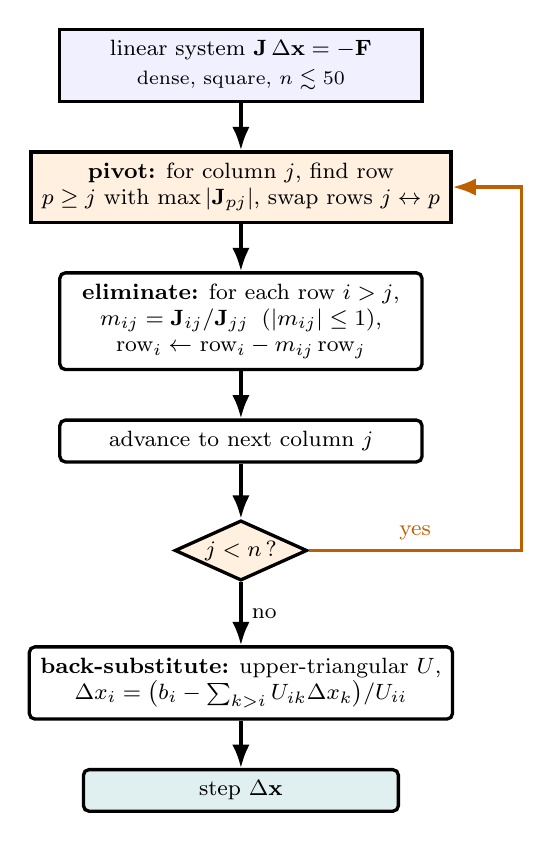
\begin{tikzpicture}[
    >={Latex[width=2.2mm]},
    every node/.style={font=\footnotesize},
    node distance = 6mm and 10mm,
    box/.style  ={draw, rounded corners=2pt, very thick, align=center,
                  inner sep=4pt, minimum width=46mm},
    io/.style   ={draw, very thick, fill=blue!6, align=center,
                  inner sep=4pt, minimum width=46mm},
    piv/.style  ={draw, very thick, fill=orange!12, align=center,
                  inner sep=4pt, minimum width=46mm},
    done/.style ={draw, rounded corners=2pt, very thick, fill=teal!12,
                  align=center, inner sep=4pt, minimum width=40mm},
    flow/.style ={->, very thick},
    loop/.style ={->, very thick, orange!75!black},
]
\node[io]  (in)  {linear system $\Jac\,\Delta\xv = -\Fv$\\[1pt]
                  {\scriptsize dense, square, $n\lesssim 50$}};
\node[piv, below=of in]    (piv) {\textbf{pivot:} for column $j$, find row\\
                  $p\ge j$ with $\max|\Jac_{pj}|$, swap rows $j\leftrightarrow p$};
\node[box, below=of piv]   (elim){\textbf{eliminate:} for each row $i>j$,\\
                  $m_{ij}=\Jac_{ij}/\Jac_{jj}$\;\;($|m_{ij}|\le 1$),\\
                  row$_i \leftarrow$ row$_i - m_{ij}\,$row$_j$};
\node[box, below=of elim]  (col) {advance to next column $j$};
\node[draw, diamond, aspect=2.2, very thick, fill=orange!12,
      below=7mm of col, inner sep=1pt, align=center] (test) {$j<n$\,?};
\node[box, below=8mm of test] (back)
     {\textbf{back-substitute:} upper-triangular $U$,\\
      $\Delta x_i=\bigl(b_i-\sum_{k>i}U_{ik}\Delta x_k\bigr)/U_{ii}$};
\node[done, below=of back]  (out) {step $\Delta\xv$};
\draw[flow] (in)   -- (piv);
\draw[flow] (piv)  -- (elim);
\draw[flow] (elim) -- (col);
\draw[flow] (col)  -- (test);
\draw[flow] (test) -- node[right]{no} (back);
\draw[flow] (back) -- (out);
\draw[loop] (test.east) -- ++(2.7,0) node[midway,above]{yes}
            |- (piv.east);
\end{tikzpicture}
\caption{Gauss elimination with partial pivoting --- the $\sim\!60$-line
direct solver that every Newton step in the simulator calls to turn
$\Jac\,\Delta\xv=-\Fv$ into a step.  Column by column it first
\emph{pivots} (swaps in the row with the largest entry in the active
column, the orange box) so the multipliers $m_{ij}$ never exceed one in
magnitude --- the guard against round-off blow-up --- then \emph{eliminates}
everything below the diagonal, leaving an upper-triangular system.  When
the last column is reached, one \emph{back-substitution} sweep reads off
$\Delta\xv$ from the bottom up.  No matrix inverse is ever formed: the
factorisation is both cheaper ($O(n^3/3)$) and steadier than $\Jac^{-1}$.}
\label{fig:lu-gauss-flow}
\end{figure}

current pivot row with whichever row below has the largest absolute
entry in the pivot column.  This keeps the multipliers $\le 1$ in
magnitude and prevents catastrophic growth of round-off in the
elimination.  Without pivoting, a Jacobian with widely varying
entries can produce numerically meaningless results.

\subsection{Damping by backtracking line search}

The full Newton step ($\lambda = 1$) is correct to second order in
$\Delta\xv$.  Far from the root, second-order error can be huge and
$\xv_k + \Delta\xv$ can land somewhere worse than $\xv_k$ --- in
chemistry, ``worse'' often means a non-physical state (negative
concentration, pressure below the saturation curve, temperature
outside the Antoine range).  The fix is the same as in 1-D
(\S\ref{ch:nr1d}, Damping): try $\lambda = 1$; if
$\|\Fv(\xv_{k+1})\|_2^2$ does not decrease, halve $\lambda$ and try
again, down to a minimum $\lambda_{\min} \sim 2^{-10}$.

\begin{intuition}
The Jacobian decides \emph{which direction} to walk; damping decides


\emph{how far} to walk in that direction.  When the linear model is
trustworthy --- close to the root, where higher-order terms are
small --- $\lambda \to 1$ and Newton recovers its quadratic-doubling
speed.  When the linear model is not trustworthy --- far from the
root, or in a region where $\Jac$ is nearly singular --- $\lambda$
shrinks until the step is short enough to stay in a safe basin.
\end{intuition}

\begin{figure}[ht]
\centering
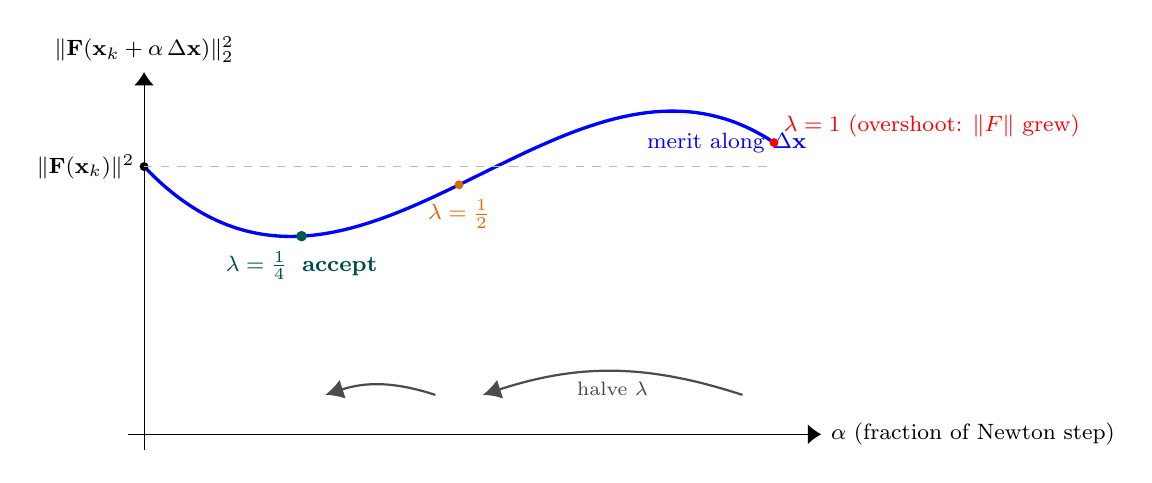
\begin{tikzpicture}[
    >={Latex[width=2.5mm]},
    every node/.style={font=\footnotesize},
    scale=1.0,
]
% merit phi(alpha) = ||F(x + alpha d)||^2 along the Newton direction.
% axes
\draw[->] (-0.2,0) -- (8.6,0) node[right] {$\alpha$ (fraction of Newton step)};
\draw[->] (0,-0.2) -- (0,4.6) node[above] {$\|\Fv(\xv_k+\alpha\,\Delta\xv)\|_2^2$};
% the merit slice along the search direction (wiggly: overshoot region rises)
\draw[blue, very thick, smooth] plot[domain=0:8, samples=80]
    (\x, {3.4 - 1.05*\x + 0.36*\x*\x - 0.028*\x*\x*\x});
\node[blue] at (7.4,3.7) {merit along $\Delta\xv$};
% value at x_k (alpha=0)
\filldraw[black] (0,3.4) circle (1.4pt);
\node[left] at (0,3.4) {$\|\Fv(\xv_k)\|^2$};
\draw[gray!55,dashed] (0,3.4) -- (8,3.4);
% full step alpha = 8 (=1 in real units) -> worse than start
\filldraw[red] (8,{3.4-1.05*8+0.36*64-0.028*512}) circle (1.4pt);
\node[red, above right] at (8,3.65) {$\lambda=1$ (overshoot: $\|F\|$ grew)};
% alpha = 4 (=1/2): still slightly worse / marginal
\filldraw[orange!85!black] (4,{3.4-1.05*4+0.36*16-0.028*64}) circle (1.4pt);
\node[orange!85!black, below=2pt] at (4,{3.4-1.05*4+0.36*16-0.028*64}) {$\lambda=\tfrac12$};
% alpha = 2 (=1/4): accepted, below current
\filldraw[teal!70!black] (2,{3.4-1.05*2+0.36*4-0.028*8}) circle (1.7pt);
\node[teal!60!black, below=2pt] at (2,{3.4-1.05*2+0.36*4-0.028*8}) {$\lambda=\tfrac14$ \;\textbf{accept}};
% halving arrows from full step back toward accepted
\draw[->, gray!60!black, thick] (7.6,0.5) to[bend right=18]
    node[midway, below, font=\scriptsize, text=gray!55!black] {halve $\lambda$} (4.3,0.5);
\draw[->, gray!60!black, thick] (3.7,0.5) to[bend right=18] (2.3,0.5);
\end{tikzpicture}
\caption{Backtracking damping seen as a one-dimensional slice of the
residual norm \emph{along} the fixed Newton direction $\Delta\xv$.  The
Jacobian has already chosen the direction; damping only chooses how far.
The full step ($\lambda=1$, red) overshoots into a region where
$\|\Fv\|^2$ is \emph{larger} than at $\xv_k$ --- in chemistry often a
non-physical state.  The simulator halves $\lambda$ ($1\to\tfrac12\to
\tfrac14$) until the trial point drops below the dashed
current-residual line (the sufficient-decrease test), and accepts the
first $\lambda$ that does.  Near the root the curve is monotone down
from $\alpha=0$, the first try $\lambda=1$ passes, and quadratic
convergence is recovered untouched.}
\label{fig:newton-damping-backtrack}
\end{figure}

\subsection{Worked example: a $2\times 2$ system}

\begin{example}[Two coupled algebraic equations]
Solve the system
\[
   F_1(\xv) \;=\; x_1^2 + x_2^2 - 5 \;=\; 0,
   \qquad
   F_2(\xv) \;=\; x_1 x_2 - 2 \;=\; 0.
\]
The pair has solutions $(2,1)$ and $(1,2)$ (and the two reflections
through the origin).  We seek $(2,1)$ from the initial guess
$\xv_0 = (2.5, 0.5)$.

\textbf{Step 1.}  Evaluate $\Fv$ and $\Jac$:
\[
   \Fv(\xv_0) = \begin{pmatrix} 2.5^2 + 0.5^2 - 5 \\ 2.5 \cdot 0.5 - 2\end{pmatrix}
              = \begin{pmatrix} 1.50 \\ -0.75 \end{pmatrix},
   \quad
   \Jac(\xv_0) = \begin{pmatrix} 2 x_1 & 2 x_2 \\ x_2 & x_1 \end{pmatrix}\!\bigg|_{\xv_0}
              = \begin{pmatrix} 5.0 & 1.0 \\ 0.5 & 2.5 \end{pmatrix}.
\]
Solve $\Jac \, \Delta\xv = -\Fv$:
\[
   \begin{pmatrix} 5.0 & 1.0 \\ 0.5 & 2.5 \end{pmatrix}
   \begin{pmatrix} \Delta x_1 \\ \Delta x_2 \end{pmatrix}
   \;=\; \begin{pmatrix} -1.50 \\ 0.75 \end{pmatrix}.
\]
Gauss elimination: pivot row 1, multiplier $0.5/5.0 = 0.1$.  Subtract
$0.1$ times row 1 from row 2: row 2 becomes
$(0, 2.4 \mid 0.90)$.  Back-substitute:
$\Delta x_2 = 0.375$,
$\Delta x_1 = (-1.50 - 1.0\cdot 0.375)/5.0 = -0.375$.
So $\xv_1 = (2.5, 0.5) + (-0.375, +0.375) = (2.125, 0.875)$.

\textbf{Step 2.}  $\Fv(\xv_1) = (0.281, -0.141)$, with
$\|\Fv\|_2 = 0.314$ (down from $1.677$); take another Newton step.
After it, $\xv_2 \approx (2.012, 0.988)$, $\|\Fv\|_2 \approx 0.025$.
Two more steps recover machine precision.  The error is squaring
roughly each iteration --- the expected quadratic convergence of
Newton near the root.
\end{example}


\begin{figure}[ht]
\centering
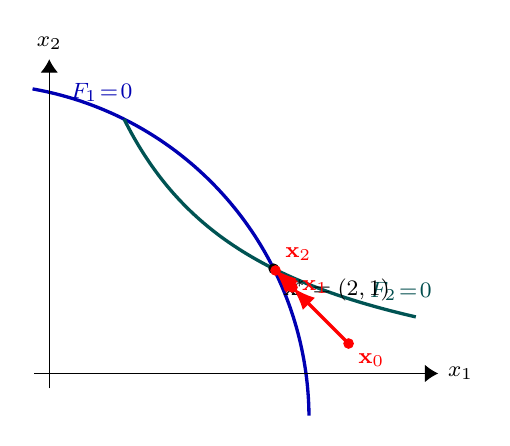
\begin{tikzpicture}[
    >={Latex[width=2.2mm]},
    every node/.style={font=\footnotesize},
    scale=1.9,
]
% Worked 2x2: F1 = x1^2+x2^2-5, F2 = x1 x2 - 2, root (2,1).
% circle x1^2+x2^2=5 (radius sqrt5 ~ 2.236) -- arc in the region shown
\draw[blue!70!black, very thick, domain=0.45:80, samples=60, smooth, variable=\t]
    plot ({2.2360679*cos(\t)}, {2.2360679*sin(\t)});
\node[blue!70!black] at (0.85,2.18) {$F_1\!=\!0$};
% hyperbola x1 x2 = 2  ->  x2 = 2/x1
\draw[teal!65!black, very thick, domain=1.0:2.95, samples=60, smooth, variable=\x]
    plot (\x, {2/\x});
\node[teal!60!black] at (2.85,0.85) {$F_2\!=\!0$};
% root
\filldraw[black] (2,1) circle (0.9pt);
\node[below right] at (2.0,1.0) {$\xv^{\!*}=(2,1)$};
% iteration path: x0=(2.5,0.5) -> x1=(2.125,0.875) -> x2=(2.012,0.988) -> root
\coordinate (x0) at (2.5,0.5);
\coordinate (x1) at (2.125,0.875);
\coordinate (x2) at (2.012,0.988);
\filldraw[red] (x0) circle (0.9pt) node[below right, text=red] {$\xv_0$};
\filldraw[red] (x1) circle (0.9pt) node[right, text=red] {$\xv_1$};
\filldraw[red] (x2) circle (0.9pt) node[above right, text=red] {$\xv_2$};
\draw[->, red, very thick] (x0) -- (x1);
\draw[->, red, very thick] (x1) -- (x2);
\draw[->, red, very thick] (x2) -- (2,1);
% axes
\draw[->] (0.4,0.3) -- (3.1,0.3) node[right] {$x_1$};
\draw[->] (0.5,0.2) -- (0.5,2.4) node[above] {$x_2$};
\end{tikzpicture}
\caption{The two Newton steps of the worked $2\times 2$ example, drawn
in the $(x_1,x_2)$ plane.  The two residual equations each define a
zero-curve --- a circle ($F_1\!=\!x_1^2\!+\!x_2^2\!-\!5\!=\!0$, blue) and
a hyperbola ($F_2\!=\!x_1x_2\!-\!2\!=\!0$, teal) --- and the root is where
they cross.  Each Newton step solves $\Jac\,\Delta\xv=-\Fv$ for a step
\emph{direction}, and the iterates $\xv_0\!\to\!\xv_1\!\to\!\xv_2$ march
straight at the intersection, the gap to $\xv^{\!*}$ roughly squaring
every step (quadratic convergence).  The same picture in $n$ dimensions
is a path on the intersection of $n$ residual hypersurfaces --- only the
drawing gets harder, never the algorithm.}
\label{fig:newtonnd-path}
\end{figure}


% ---------------------------------------------------------------------
\section{Parameter estimation: Levenberg-Marquardt}\label{ch:lm}

\begin{whatyoulllearn}
How the simulator turns a table of experimental bubble-temperature
data into a fitted set of NRTL (or Wilson) interaction parameters.
We will derive each piece from scratch: why \emph{least squares}; why
the gradient of $\chi^2$ is exactly $\Jac^{\!\top}\rv$; why its
Hessian splits into two terms and why one of them can be dropped;
how the resulting Gauss-Newton step can overshoot; Levenberg's
damping fix; Marquardt's invariance fix; and the simple
trust-region rule the simulator uses to update the damping. The
runnable case is \file{tutorials/fitNRTL01\_ethanol\_water/}.
\end{whatyoulllearn}

\subsection{A different question}

Every solver in Part~III so far has had the same shape: \emph{given
a model, find the inputs that satisfy a residual.} Flash,
bubble-$T$, CSTR, distillation --- all instances of "solve
$\Fv(\xv) = 0$".

Parameter estimation flips the question. We have:
\begin{itemize}[leftmargin=*,nosep]
  \item a \emph{model with adjustable knobs} --- here, NRTL with its
        four binary-interaction parameters $a_{ij}, b_{ij}, a_{ji},
        b_{ji}$ (the $\alpha_{ij}$ non-randomness is held fixed by
        convention);
  \item a \emph{table of experimental data} that the model should
        reproduce --- here, $N$ pairs $(x^{\mathrm{exp}}_i,
        T^{\mathrm{exp}}_i)$ at fixed pressure $P$;
  \item and we want to find the knob setting that makes the model
        agree with the data as closely as possible.
\end{itemize}
This is an \emph{over-determined} problem: $N \gg m$, so we cannot
satisfy every data point exactly, only minimise the total mismatch.

\subsection{Problem statement}

Let $\pv \in \R^m$ be the parameter vector (for an NRTL binary,
$m = 4$: $a_{ij}, b_{ij}, a_{ji}, b_{ji}$). The simulator provides
a \emph{forward model}: for each experimental composition
$x^{\mathrm{exp}}_i$, run a bubble-$T$ calculation with the current
$\pv$ and return the predicted temperature,
\begin{equation}
   T_i^{\mathrm{pred}}(\pv) \;=\; \text{bubble-}T\text{ at }
   (x^{\mathrm{exp}}_i,\,1 - x^{\mathrm{exp}}_i,\,P)\text{ with NRTL}(\pv).
\end{equation}
The \textbf{residual} at point $i$ is the prediction error,
\begin{equation}
   r_i(\pv) \;\equiv\; T_i^{\mathrm{pred}}(\pv) - T_i^{\mathrm{exp}},
\end{equation}
and we minimise the sum of squared residuals,
\begin{equation}
   \boxed{\;
   \chi^2(\pv) \;\equiv\; \tfrac{1}{2}\sum_{i=1}^{N} r_i(\pv)^2
                 \;=\; \tfrac{1}{2}\,\rv(\pv)^{\!\top}\rv(\pv).
   \;}
   \label{eq:chi2}
\end{equation}

\begin{intuition}
Why squared, not absolute value or fourth power? Squaring is the
unique choice that is everywhere differentiable, penalises large
mismatches disproportionately (so a single outlier still pulls the
fit), and is the maximum-likelihood estimator when the experimental
errors are independent Gaussians of equal variance. The factor
$\tfrac{1}{2}$ is bookkeeping --- it cancels the $2$ that drops out
of $\frac{d}{dp_j}(r_i^2) = 2\,r_i\,\partial r_i/\partial p_j$ in
the gradient.
\end{intuition}

\subsection{The gradient of $\chi^2$: deriving $\Jac^{\!\top}\rv$}

At a minimum, every partial derivative of $\chi^2$ vanishes. Let us
compute $\partial\chi^2/\partial p_j$ explicitly. Using the chain
rule on Eq.~\eqref{eq:chi2},
\begin{equation}
   \frac{\partial \chi^2}{\partial p_j}
   \;=\; \frac{\partial}{\partial p_j}\Bigl[\tfrac{1}{2}\sum_{i=1}^{N} r_i^2\Bigr]
   \;=\; \tfrac{1}{2}\sum_{i=1}^{N} 2\,r_i\,\frac{\partial r_i}{\partial p_j}
   \;=\; \sum_{i=1}^{N} r_i\,\frac{\partial r_i}{\partial p_j}.
\end{equation}
Now collect the partial derivatives of the residual into the
\textbf{residual Jacobian}
\begin{equation}
   \Jac_{ij}(\pv) \;\equiv\; \frac{\partial r_i}{\partial p_j},
   \qquad \Jac \in \R^{N \times m},
\end{equation}
so that the $j$-th component of the gradient is exactly
$\sum_i r_i \Jac_{ij} = (\Jac^{\!\top}\rv)_j$. Stacking all $m$
partials:
\begin{equation}
   \boxed{\;
   \nabla_{\pv}\chi^2(\pv) \;=\; \Jac(\pv)^{\!\top}\,\rv(\pv).
   \;}
\end{equation}
A minimum therefore satisfies $\Jac^{\!\top}\rv = 0$, the
\emph{normal-equation condition}. This is the same shape of system
we have already met: $m$ equations, $m$ unknowns. The natural thing
to do is run a Newton iteration on it.

\subsection{The Hessian splits in two: keep one piece, drop the other}

To apply Newton-Raphson to $\nabla\chi^2 = 0$ we need the Hessian
$\nabla^2\chi^2 \in \R^{m\times m}$. Differentiate
$(\Jac^{\!\top}\rv)_j = \sum_i r_i\,\partial r_i/\partial p_j$ once
more, with respect to $p_k$:
\begin{equation}
   \frac{\partial^2 \chi^2}{\partial p_j \partial p_k}
   \;=\; \sum_{i=1}^{N}
        \frac{\partial r_i}{\partial p_k}\,\frac{\partial r_i}{\partial p_j}
        \;+\;
        \sum_{i=1}^{N} r_i\,\frac{\partial^2 r_i}{\partial p_j \partial p_k}.
\end{equation}
In matrix form,
\begin{equation}
   \nabla^2 \chi^2
   \;=\;
   \underbrace{\Jac^{\!\top}\Jac}_{\text{first-derivative information}}
   \;+\;
   \underbrace{\sum_{i=1}^{N} r_i\,\nabla^2 r_i}_{\text{second-derivative information}}.
   \label{eq:hessian-split}
\end{equation}
The first term costs us nothing extra --- we already have $\Jac$.
The second term requires the $m\times m$ Hessian of every single
residual: $N$ matrices of $m^2$ second partials, each obtained
from forward model calls. Forming it by finite differences would
multiply the cost of one LM iteration by roughly a factor of $m$.

The \emph{Gauss-Newton approximation} is to drop the second term:
\begin{equation}
   \nabla^2 \chi^2 \;\approx\; \Jac^{\!\top}\Jac.
\end{equation}

\begin{intuition}
Why is dropping $\sum_i r_i \nabla^2 r_i$ defensible? Look at the
sum: it is weighted by the residuals themselves. At the optimum
$\pv^*$ the residuals are small (the whole point of the fit), so
the dropped term is small \emph{compared to} $\Jac^{\!\top}\Jac$
(which is a sum of squares and grows with $N$). Near $\pv^*$,
$r_i$ errors of $\sim 0.4$~K with a $\Jac$ whose columns have norm
$\sim 1$ make the dropped term roughly $100\times$ smaller than the
kept one. Far from $\pv^*$ the approximation can mislead --- and
that is exactly where Levenberg's damping (next subsection) saves
us.
\end{intuition}

With the Gauss-Newton Hessian, Newton-Raphson on
$\nabla\chi^2 = 0$ becomes
\begin{equation}
   \bigl(\Jac^{\!\top}\Jac\bigr)\,\Delta\pv \;=\; -\Jac^{\!\top}\rv,
   \qquad \pv_{k+1} \;=\; \pv_k + \Delta\pv.
   \label{eq:normal-eq}
\end{equation}
This $m\times m$ linear system is the \textbf{normal equations} of
the linear least-squares problem
$\min_{\Delta\pv}\|\rv + \Jac\,\Delta\pv\|^2$. You can read it
either way: as a Newton step on $\nabla\chi^2 = 0$ (the derivation
above), or as the closed-form minimiser of the linearised residual
$\rv(\pv + \Delta\pv) \approx \rv + \Jac\,\Delta\pv$.

\begin{pitfall}
Gauss-Newton is locally a descent direction for $\chi^2$, but only
\emph{locally}. If the linearisation $\rv(\pv + \Delta\pv) \approx
\rv + \Jac\,\Delta\pv$ is poor --- because we are far from
$\pv^*$, or some $r_i$ are large, or the residual surface curves
sharply --- the full Gauss-Newton step can overshoot wildly and
\emph{increase} $\chi^2$. You will see this in the simulator's LM
trace as iterations where the trial $\chi^2$ jumps by orders of
magnitude before being rolled back.
\end{pitfall}

\subsection{Levenberg's idea: a knob between two extremes}

We have two algorithms in hand to minimise $\chi^2$, with opposite
failure modes:
\begin{itemize}[leftmargin=*,nosep]
  \item \textbf{Gauss-Newton}, Eq.~\eqref{eq:normal-eq}, takes
        \emph{long} steps in the direction the linearised model
        prefers. Near $\pv^*$ it converges quadratically. Far from
        $\pv^*$ it overshoots.
  \item \textbf{Steepest descent}, $\Delta\pv = -\alpha\,\nabla\chi^2
        = -\alpha\,\Jac^{\!\top}\rv$, takes \emph{short} steps in
        the direction $\chi^2$ decreases fastest. It provably
        reduces $\chi^2$ for a small enough $\alpha$. But near
        $\pv^*$ it zigzags through narrow valleys and crawls.
\end{itemize}
Levenberg \cite{Levenberg44} proposed to interpolate between the
two by adding a tunable damping term to the normal-equation matrix:
\begin{equation}
   \bigl(\Jac^{\!\top}\Jac + \lambda\,\mathbf{I}\bigr)\,\Delta\pv
   \;=\; -\Jac^{\!\top}\rv.
   \label{eq:levenberg}
\end{equation}
The two limits of the $\lambda$-knob are illuminating:
\begin{itemize}[leftmargin=*,nosep]
  \item $\lambda \to 0$: the damping vanishes and the system reduces
        to Eq.~\eqref{eq:normal-eq} --- pure Gauss-Newton, with
        local quadratic convergence.
  \item $\lambda \to \infty$: the damping term dominates and
        $\Delta\pv \approx -\lambda^{-1}\,\Jac^{\!\top}\rv =
        -\lambda^{-1}\,\nabla\chi^2$ --- an arbitrarily short step
        along the steepest-descent direction. Linear convergence,
        but \emph{guaranteed} to decrease $\chi^2$ if the step is
        short enough.
\end{itemize}
Notice the dual role $\lambda$ plays. Increasing it does not only
\emph{rotate} the step toward the gradient: it also \emph{shrinks}
the step, because the diagonal of $\Jac^{\!\top}\Jac +
\lambda\mathbf{I}$ grows and divides $\Delta\pv$ down. That is why
$\lambda$ doubles as an implicit trust-region radius: big $\lambda$
means "I do not trust the linear model out to a long step, take a
short careful one."

\subsection{Marquardt's invariance fix}

Levenberg's $\lambda\,\mathbf{I}$ has a subtle defect: it is not
invariant under a diagonal rescaling of the parameters. Suppose we
re-expressed every $p_j$ in units that doubled it: $p_j \to 2 p_j$.
The columns of $\Jac$ would halve, $\Jac^{\!\top}\Jac$ would scale
by $1/4$ along its diagonal, but $\lambda\mathbf{I}$ would not
change. A $\lambda$ that was small compared to one diagonal entry
of $\Jac^{\!\top}\Jac$ might now dominate it.

For NRTL parameters this matters in practice: $a_{ij}$ is a
dimensionless $\mathcal{O}(1)$ number, but $b_{ij}$ carries units
of K and runs $\mathcal{O}(100\text{--}1000)$. A single $\lambda$
that damps the $b$ direction reasonably will completely lock the
$a$ direction (or vice versa).

Marquardt \cite{Marquardt63} fixed this by scaling the damping
with the diagonal of $\Jac^{\!\top}\Jac$ itself:
\begin{equation}
   \boxed{\;
   \bigl(\Jac^{\!\top}\Jac + \lambda\,\diag(\Jac^{\!\top}\Jac)\bigr)\,\Delta\pv
   \;=\; -\Jac^{\!\top}\rv.
   \;}
   \label{eq:marquardt}
\end{equation}
This is invariant under diagonal reparametrisation: doubling all
$b_{ij}$ shrinks both terms in the matrix by the same factor, so
their relative weighting is preserved.

The simulator implements Eq.~\eqref{eq:marquardt} in the
\emph{multiplicative} form that is common in practice: each
diagonal entry of $\Jac^{\!\top}\Jac$ is multiplied by $1 +
\lambda$. That is the same equation with the $\lambda$ knob
shifted by one --- $\lambda = 0$ in the multiplicative form is
pure Gauss-Newton; $\lambda \to \infty$ is pure scaled gradient
descent.

\begin{intuition}
The diagonal entry $(\Jac^{\!\top}\Jac)_{jj} = \sum_i (\partial
r_i / \partial p_j)^2$ is the local curvature of $\chi^2$ along
the $p_j$ axis --- the second derivative of $\chi^2$ in direction
$j$, in the Gauss-Newton approximation. Damping in proportion to
this curvature means: take small steps in well-determined (stiff)
parameter directions, take longer steps in poorly-determined
(slack) ones. Without the scaling, one fixed $\lambda$ ends up
calibrated for the stiffest direction and is needlessly
conservative everywhere else --- which is what makes plain
Levenberg's convergence so unsteady on real problems.
\end{intuition}

\subsection{The trust-region update: 3 down, 5 up}

The damping $\lambda$ is not fixed --- it is adjusted every
iteration based on whether the proposed step \emph{actually}
decreased $\chi^2$. The logic is simple:
\begin{itemize}[leftmargin=*,nosep]
  \item If $\chi^2(\pv_k + \Delta\pv) < \chi^2(\pv_k)$, the
        linearisation was good enough. \emph{Accept} the step
        ($\pv_{k+1} = \pv_k + \Delta\pv$) and \emph{shrink}
        $\lambda$ to push toward Gauss-Newton next time. The
        simulator uses $\lambda \leftarrow \lambda / 3$.
  \item Otherwise the linearisation overshot. \emph{Reject} the
        step ($\pv_{k+1} = \pv_k$) and \emph{grow} $\lambda$ to
        take a shorter, more gradient-aligned step next time. The
        simulator uses $\lambda \leftarrow 5\,\lambda$.
\end{itemize}

\begin{intuition}
Read $\lambda$ as a trust-region radius: small $\lambda$ = "I
trust the linear model out to a long step"; large $\lambda$ = "I
do not, keep close to the current $\pv$." Each LM iteration is
one experiment that tests how far the linear model can be
trusted; the trust radius shrinks or grows based on the
experimental outcome. This is the single algorithmic ingredient
that distinguishes LM from plain Gauss-Newton --- and it is the
reason LM converges on problems where Gauss-Newton diverges.
\end{intuition}

The 3-down/5-up asymmetry is conservative on purpose: a rejected
step has already cost a full Jacobian rebuild ($2m$ extra forward
solves), so we want to avoid the \emph{next} rejection more
aggressively than we want to chase Gauss-Newton speed. The exact
factors are tunable; $3$ and $5$ follow Press \textit{et al.}
\cite{NumericalRecipes} with one click more caution.

\subsection{Finite-difference Jacobian}

The model $T_i^{\mathrm{pred}}(\pv)$ is a black-box solver call,
not a closed-form expression. We compute $\Jac$ by central
differences in $\pv$:
\begin{equation}
   \Jac_{ij}(\pv)
   \;\approx\;
   \frac{r_i(\pv + h_j\,\mathbf{e}_j) - r_i(\pv - h_j\,\mathbf{e}_j)}{2\,h_j},
\end{equation}
with a relative step
\begin{equation}
   h_j \;=\; \epsilon_{\mathrm{rel}}\,\max(1, |p_j|),
   \qquad
   \epsilon_{\mathrm{rel}} \;=\; 10^{-4}.
\end{equation}
Each column of $\Jac$ costs $2$ forward solves of the simulator. For
the canonical ethanol-water case ($m=4$ parameters, $N=11$ data
points), one LM iteration is therefore $1 + 2\,m = 9$ vector forward
evaluations, each of which loops over $N$ bubble-$T$ calls.

\begin{pitfall}
The step size $h_j$ has two error sources working against each other:
\textbf{truncation error} (the second derivative we ignore in the FD
formula) grows as $h^2$; \textbf{round-off error} grows as
$\epsilon_{\mathrm{machine}} / h$ for an arithmetic resembling double
precision. The optimum is near $h \sim \epsilon_{\mathrm{machine}}^{1/3}
\approx 10^{-5}$ for central differences. The simulator's $10^{-4}$ is a
shade larger --- chosen because the inner bubble-$T$ solve is itself
accurate to about $10^{-8}$~K, so a smaller $h$ would not buy more
accuracy and would amplify the inner solver's noise.
\end{pitfall}

\subsection{Stopping criteria}

The LM loop exits successfully when the relative improvement in
$\chi^2$ falls below \code{tolerance} (default $10^{-6}$):
\begin{equation}
   \frac{\chi^2_{k-1} - \chi^2_k}{\chi^2_{k-1}}
   \;<\; \texttt{tolerance}.
\end{equation}
It exits unsuccessfully on either \code{maxIter} iterations (default
$30$) or a damping blow-up $\lambda > 10^{10}$, which signals that the
trust region has collapsed --- the Hessian approximation is indefinite
or the residual surface is too non-smooth for the FD Jacobian. In
practice the second failure mode shows up when the dataset contains
near-duplicate $x_i$ values or when the initial guess is so far from
$\pv^*$ that the inner bubble-$T$ Newton itself fails to converge.

\subsection{The simulator's implementation}

The operation is registered as \code{type fitParameters;} in
\file{system/propsDict} (its choupoSolve-era predecessor
\code{fitBinaryPair} is retired --- the factory throws, naming the
replacement).  Its main loop lives in
\file{src/propertyOps/FitParameters.cpp}, which calls into:
\begin{itemize}[leftmargin=*,nosep]
  \item \code{Dictionary::setScalarAtPath()} to overwrite the four
        NRTL parameters in \code{thermoDict\_} for each forward
        evaluation;
  \item the existing \code{BubblePoint} unit-op (which emits
        \code{T\_bubble} as a KPI from onwards) for the inner
        bubble-$T$;
  \item \code{solver::gaussSolve} (the same Gauss elimination used by
        \code{NewtonND}, just on the $4\times 4$ normal-equations
        system).
\end{itemize}
No external library, no auto-differentiation, no hand-coded analytical
Jacobian: a deliberate constraint for pedagogical visibility.

\begin{tutoriallink}
\code{runCase tutorials/fitNRTL01\_ethanol\_water} produces the full
LM trace, the per-point residual breakdown, and writes the proposal
file \code{constant/binaryPairs/NRTL/ethanol-water.fit-<date>.dat}.
See the case's \file{README.md} for the promote-by-\code{mv} step.
\end{tutoriallink}

\begin{example}[Reading the LM trace for ethanol-water at 1\,atm]
The simulator prints one row per iteration:
\begin{lstlisting}[basicstyle=\ttfamily\scriptsize]
  iter     chi^2          RMS(K)     lambda    step
  ----  ------------  ----------  --------  --------
  init  6.0195e+01    2.3393e+00  1.0e-03               (DECHEMA literature)
  1     54.0505       2.2167      1.0e-03   523.9       (accepted, lambda /= 3)
  2     17990.5239    40.4413     3.3e-04   0.0009      (REJECTED, lambda *= 5)
  3     6020.4407     23.3947     1.7e-03   0.0009      (REJECTED)
...
  18    1.8006        0.4046      4.5e+00   6.8971      (accepted)
  19    6109.9721     23.5680     1.5e+00   0.0000      (REJECTED)
  20    1.8006        0.4046      7.4e+00   0.0000      (converged: rel<tol)
\end{lstlisting}
Read row by row:
\begin{itemize}[leftmargin=*,nosep]
  \item \textbf{Initial $\chi^2 = 60.2$, RMS $= 2.34$~K.} With the
        literature DECHEMA parameters, the model overpredicts $T_b$
        by about $2$~K on average across this dataset.
  \item \textbf{Iter 1 ($\lambda = 10^{-3}$):} small damping, pure
        Gauss-Newton step. $\chi^2$ drops marginally; step norm is
        large ($\sim 524$) --- the gradient was steep.
  \item \textbf{Iter 2 ($\lambda = 3.3 \times 10^{-4}$):} the previous
        step shrank $\lambda$, so the next is even more Gauss-Newton-ish.
        But the linearisation no longer holds at this displaced point;
        $\chi^2$ rockets to $1.8\times 10^4$. \emph{Rejected};
        $\lambda$ jumps to $1.7\times 10^{-3}$.
  \item \textbf{Iters 3--17:} the loop oscillates between accept (with
        $\lambda$ decreasing 3-fold) and reject (with $\lambda$
        increasing 5-fold). $\chi^2$ drifts down on the accept
        rows. The \texttt{step} column shrinks as the active subspace
        of $\pv$ narrows.
  \item \textbf{Iter 18:} an accepted step that drops $\chi^2$ to
        $1.80$, RMS $= 0.40$~K. Five-fold improvement over literature
        for THIS dataset.
  \item \textbf{Iter 19:} a final overreach, rejected.
  \item \textbf{Iter 20:} same $\chi^2$ as iter 18, but with the
        relative improvement now $< 10^{-6}$. Converged.
\end{itemize}
The lesson visible in the trace: the trust region tightens the more
non-linear the residual surface is around the current $\pv$, and
relaxes when the linearisation holds. That dance is exactly what
distinguishes LM from plain Gauss-Newton --- the latter would have
diverged at iteration~2.
\end{example}

% --- Figure: LM convergence (real data from fitNRTL01) -----------------
\begin{figure}[h]
\centering
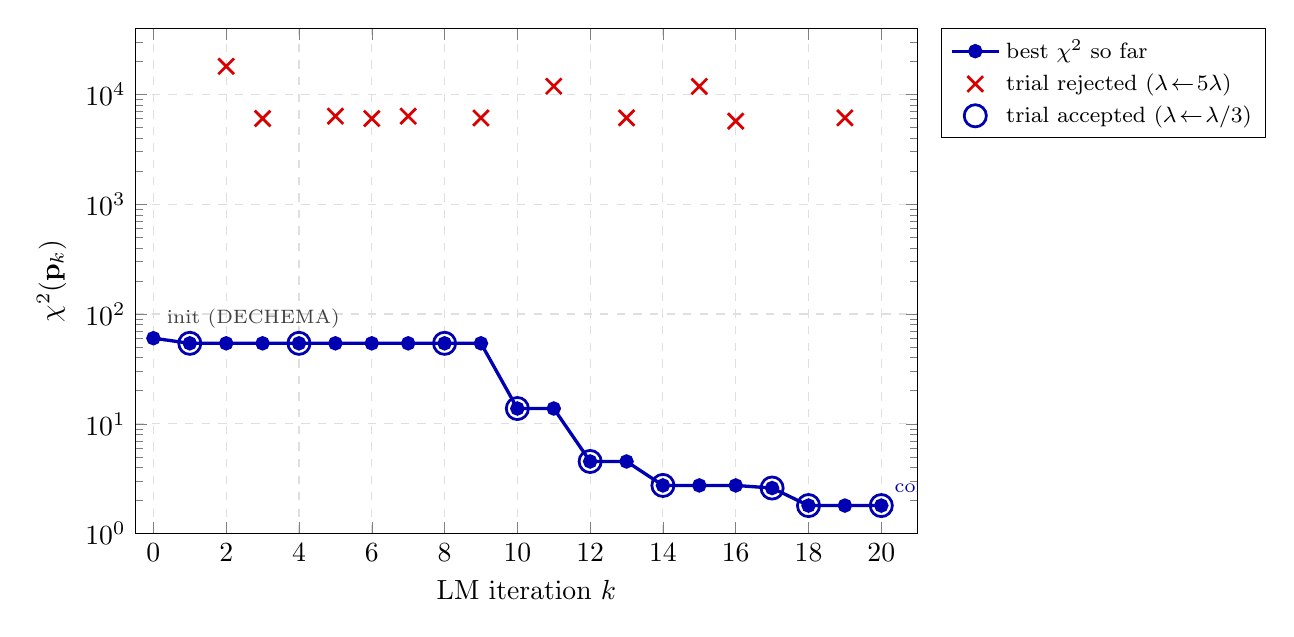
\begin{tikzpicture}
\begin{semilogyaxis}[
    width=0.95\linewidth, height=8cm,
    xlabel={LM iteration $k$},
    ylabel={$\chi^2(\pv_k)$},
    xmin=-0.5, xmax=21,
    ymin=1, ymax=40000,
    grid=major,
    grid style={gray!25, dashed},
    legend pos=outer north east,
    legend cell align=left,
    legend style={font=\footnotesize},
    title style={font=\small\bfseries},
    every axis title/.style={below=1ex, at={(0.5,1)}, anchor=south},
]
% (1) Best-so-far chi^2 — the actual convergence curve
\addplot[blue!70!black, very thick, mark=*, mark size=2pt] coordinates {
    (0, 60.195) (1, 54.0505) (2, 54.0505) (3, 54.0505) (4, 54.0479)
    (5, 54.0479) (6, 54.0479) (7, 54.0479) (8, 54.0460) (9, 54.0460)
    (10, 13.7763) (11, 13.7763) (12, 4.5377) (13, 4.5377) (14, 2.7461)
    (15, 2.7461) (16, 2.7461) (17, 2.6001) (18, 1.8006) (19, 1.8006)
    (20, 1.8006)
};
\addlegendentry{best $\chi^2$ so far}
% (2) Rejected trials (chi^2_trial > best, lambda *= 5 next)
\addplot[only marks, mark=x, mark size=4pt, mark options={red!85!black, line width=1.0pt}]
    coordinates {
    (2, 17990.5239) (3, 6020.4407) (5, 6327.6093) (6, 6020.4437)
    (7, 6327.6091) (9, 6095.3894) (11, 11852.3721) (13, 6105.5200)
    (15, 11802.7053) (16, 5699.2926) (19, 6109.9721)
};
\addlegendentry{trial rejected ($\lambda\!\leftarrow\!5\lambda$)}
% (3) Accepted trials (also on best line)
\addplot[only marks, mark=o, mark size=4pt, mark options={blue!70!black, line width=1.0pt}]
    coordinates {
    (1, 54.0505) (4, 54.0479) (8, 54.0460) (10, 13.7763) (12, 4.5377)
    (14, 2.7461) (17, 2.6001) (18, 1.8006) (20, 1.8006)
};
\addlegendentry{trial accepted ($\lambda\!\leftarrow\!\lambda/3$)}
\node[anchor=south west, font=\scriptsize, text=blue!70!black]
    at (axis cs:20.1, 1.8006) {converged};
\node[anchor=south west, font=\scriptsize, text=gray!50!black]
    at (axis cs:0.1, 60.195) {init (DECHEMA)};
\end{semilogyaxis}
\end{tikzpicture}
\caption{Levenberg-Marquardt $\chi^2$ history for the ethanol/water
NRTL fit in \file{tutorials/fitNRTL01\_ethanol\_water} (real run, all
20 iterations).  The solid blue line tracks the best $\chi^2$ achieved
so far --- the parameters that are carried forward.  The red crosses
are trial $\chi^2$ values the LM proposed but \emph{rejected} because
they were larger than the best, each triggering
$\lambda \leftarrow 5\lambda$.  The blue circles are the accepted
trials, each triggering $\lambda \leftarrow \lambda/3$.  The
3-up/5-down trust-region update keeps the accepted sequence monotone
even though per-iteration trials oscillate over three orders of
magnitude.}
\label{fig:lm-convergence}
\end{figure}

\begin{intuition}
Levenberg-Marquardt is best understood not as a single algorithm but
as a continuously-tuned \emph{mixture} of two limits: Gauss-Newton
(fast but fragile) and gradient descent (slow but bullet-proof). The
$\lambda$ knob slides between them automatically based on whether the
last step worked. The Marquardt diagonal scaling makes the knob
behave the same regardless of how you re-express the parameters.
\end{intuition}

% ---------------------------------------------------------------------
\section{Wegstein acceleration}\label{ch:wegstein}

\begin{whatyoulllearn}
\emph{Fixed-point} problems --- equations of the form $x = f(x)$ ---
are at the heart of every simulator's outer loops.  The naive
solution method, called \emph{direct substitution}, can be glacially
slow.  This chapter derives Wegstein's acceleration from first
principles, step by step: from the slowness of direct substitution,
to the idea of approximating $f$ as linear, to the closed-form
formula that the simulator uses for its activity-coefficient loop.
\end{whatyoulllearn}

\subsection{The setting: fixed-point problems}

A \emph{fixed-point problem} is the search for a value $x^{\!*}$
that satisfies
\begin{equation}
   x^{\!*} \;=\; f(x^{\!*}),
   \label{eq:fixed-point}
\end{equation}
where $f \colon \R \to \R$ is some function we can evaluate.
Geometrically, $x^{\!*}$ is the value where the curve $y = f(x)$
crosses the diagonal $y = x$.  In a process simulator a typical
$f$ takes a current estimate of the activity coefficients and
returns an updated estimate (we'll get to the details in
\S\ref{ch:rr} and \S\ref{ch:activity}); what matters here is the
abstract problem.

\subsection{Direct substitution and why it can be slow}

The most obvious way to solve $x = f(x)$ is to start somewhere,
plug in, and repeat:
\begin{equation}
   x_{k+1} \;=\; f(x_k),
   \qquad k = 0, 1, 2, \dots
   \label{eq:direct-sub}
\end{equation}
This is \emph{direct substitution}.  When it works, it works because
each step shrinks the error.  Let $e_k \equiv x_k - x^{\!*}$.
Linearising $f$ around $x^{\!*}$,
\[
   f(x_k) \;=\; f(x^{\!*}) + f'(x^{\!*})\,e_k + O(e_k^2)
            \;=\; x^{\!*} + f'(x^{\!*})\,e_k + O(e_k^2),
\]
so
\begin{equation}
   e_{k+1} \;=\; x_{k+1} - x^{\!*} \;=\; f'(x^{\!*})\,e_k + O(e_k^2).
\end{equation}
The error shrinks by the factor $|f'(x^{\!*})|$ each step.  If this
\emph{contraction factor} is $0.1$, ten iterations give six digits;
if it is $0.9$, ten iterations give roughly half a digit.

\begin{example}[Direct substitution on a slow problem]
Consider $f(x) = 0.9\,x + 0.5$, with fixed point $x^{\!*} = 5$ (you can
verify by substitution).  Here $f'(x) = 0.9$ everywhere, so the
contraction factor is exactly $0.9$.  Starting at $x_0 = 0$:
\[
   x_0 = 0,\;\; x_1 = 0.5,\;\; x_2 = 0.95,\;\; x_3 = 1.36,\;\;
   x_4 = 1.72,\;\; \ldots,\;\; x_{20} \approx 4.39,\;\; x_{30} \approx 4.79.
\]
After thirty iterations we are still $0.21$ away from the answer.
This kind of slow contraction is exactly what happens to the
activity-coefficient loop near an azeotrope.
\end{example}

\subsection{The Wegstein idea: model $f$ as a straight line}

Wegstein's observation \cite{Wegstein} is this: \emph{if we already
have two iterates $x_{k-1}$ and $x_k$, we know not just one point on
the curve $y = f(x)$ but \emph{two}.  Two points define a line.  We
can use that line as a local linear approximation to $f$, and solve
the linear problem $x = (\text{line})$ exactly in one step.}

\paragraph{The model.}  Approximate the curve $y = f(x)$ by the
secant line through $(x_{k-1}, f(x_{k-1}))$ and $(x_k, f(x_k))$.
Its slope is
\begin{equation}
   s_k \;\equiv\; \frac{f(x_k) - f(x_{k-1})}{x_k - x_{k-1}}.
   \label{eq:wegstein-slope}
\end{equation}
The line itself can be written, point-slope form anchored at
$(x_k, f(x_k))$, as
\[
   y \;=\; f(x_k) + s_k\,(x - x_k).
\]

\paragraph{The next iterate.}  Treat this line as if it \emph{were}
the true $f$ and solve the linear fixed-point equation $y = x$:
\[
   x \;=\; f(x_k) + s_k\,(x - x_k).
\]
Collect $x$-terms on the left,
\[
   x\,(1 - s_k) \;=\; f(x_k) - s_k\,x_k,
\]
and divide by $(1 - s_k)$:
\begin{equation}
   x_{k+1}
   \;=\; \frac{f(x_k) - s_k\,x_k}{1 - s_k}.
   \label{eq:wegstein-raw}
\end{equation}

\paragraph{Rearranging into Wegstein's form.}  Equation
\eqref{eq:wegstein-raw} is the answer, but it is rarely written this
way.  Define a single bookkeeping coefficient
\begin{equation}
   q_k \;\equiv\; \frac{s_k}{s_k - 1}
   \label{eq:wegstein-q}
\end{equation}
(so $1 - q_k = -1/(s_k - 1) = 1/(1 - s_k)$, and
$1 - q_k = 1 + 1/(1-s_k)$ when written symmetrically --- the algebra
is in the next paragraph).  Multiplying numerator and denominator of
\eqref{eq:wegstein-raw} by $-1$ and using $q_k$:
\[
   x_{k+1}
   \;=\; \frac{s_k\,x_k - f(x_k)}{s_k - 1}
   \;=\; \frac{s_k}{s_k-1}\,x_k - \frac{1}{s_k-1}\,f(x_k)
   \;=\; q_k\,x_k + (1 - q_k)\,f(x_k),
\]
because $-1/(s_k-1) = 1 - s_k/(s_k-1) = 1 - q_k$.
This is the Wegstein step:
\begin{equation}
   \boxed{\;
   x_{k+1} \;=\; q_k \, x_k + (1 - q_k) \, f(x_k),
   \quad\text{with}\quad
   q_k \;=\; \frac{s_k}{s_k-1},
   \quad
   s_k \;=\; \frac{f(x_k) - f(x_{k-1})}{x_k - x_{k-1}}.
   \;}
   \label{eq:wegstein}
\end{equation}

\paragraph{Reading the formula.}
The Wegstein step is a \emph{linear combination} of the current
iterate $x_k$ and the direct-substitution next iterate $f(x_k)$.
The coefficient $q_k$ controls the mix.  Three limiting cases give
the intuition:

\begin{itemize}[leftmargin=*,nosep,topsep=2pt]
  \item $s_k = 0$ (the function is locally flat): $q_k = 0$.
        The step becomes $x_{k+1} = f(x_k)$ --- ordinary direct
        substitution.  Makes sense: a flat $f$ has nothing to
        accelerate.
  \item $s_k \to 1^{-}$ (the contraction is becoming slow:
        $f'(x^{\!*})$ near 1): $q_k$ becomes a large negative
        number, $1 - q_k$ a large positive one.  The step throws
        the iterate far past $f(x_k)$ in the same direction.
        This is the whole point: direct substitution would take
        many steps to cover that distance; Wegstein takes one.
  \item $s_k > 1$: the secant slope is steeper than the diagonal,
        so the linear model is not a contraction at all.  The
        formula gives a positive $q_k$ that can be arbitrarily
        large, throwing the iterate in the \emph{wrong} direction.
        We will fix this in \S\ref{sec:wegstein-qclip}.
\end{itemize}

\begin{intuition}
Direct substitution says ``my next guess is wherever $f$ took me''.
Wegstein says ``$f$ is approximately linear locally; let me solve
the linear problem directly and jump straight to the answer''.
When $f$ really is linear, Wegstein hits $x^{\!*}$ in one step
(the secant is the curve itself).  When $f$ is non-linear, the
secant is only a chord; we land near $x^{\!*}$, take a new
secant from the latest two iterates, and try again.  Each round
the secant is closer to the local tangent at $x^{\!*}$, so
convergence accelerates as we close in.  This is \emph{super-linear}
convergence: the per-step error reduction itself improves over
time, unlike direct substitution's fixed contraction factor.
\end{intuition}

\subsection{A worked iteration}

Take the slow problem from the earlier example: $f(x) = 0.9\,x + 0.5$,
$x^{\!*} = 5$.  Start from two direct-substitution iterates
$x_0 = 0$ and $x_1 = f(x_0) = 0.5$.  Then:
\begin{align*}
   s_1 \;&=\; \frac{f(x_1) - f(x_0)}{x_1 - x_0}
            \;=\; \frac{0.95 - 0.5}{0.5 - 0}
            \;=\; 0.9, \\[2pt]
   q_1 \;&=\; \frac{s_1}{s_1 - 1}
            \;=\; \frac{0.9}{-0.1}
            \;=\; -9, \\[2pt]
   x_2 \;&=\; q_1\,x_1 + (1 - q_1)\,f(x_1)
            \;=\; -9 \cdot 0.5 + 10 \cdot 0.95
            \;=\; -4.5 + 9.5
            \;=\; 5.0.
\end{align*}
\emph{One} Wegstein step reaches the fixed point exactly --- whereas
direct substitution needed thirty iterations to get within $0.21$.
The miracle is that $f$ is linear, so Wegstein's linear model is
\emph{exact}, and the linear problem is solved in closed form.

% --- Figure: Wegstein secant geometric --------------------------------
\begin{figure}[h]
\centering
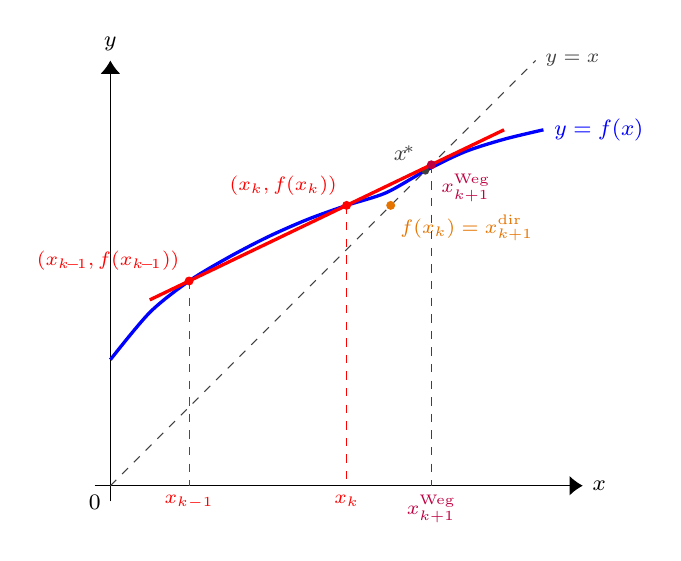
\begin{tikzpicture}[
    >={Latex[width=2.5mm]},
    every node/.style={font=\footnotesize},
    scale=2.0,
]
% Axes
\draw[->] (-0.1, 0) -- (3.0, 0) node[right] {$x$};
\draw[->] (0, -0.1) -- (0, 2.7) node[above] {$y$};
\node[below left] at (0, 0) {$0$};

% Curve y = f(x)  — a generic non-linear monotone function with fixed point at (2, 2)
\draw[blue, very thick, smooth] plot coordinates {
    (0, 0.80) (0.25, 1.10) (0.50, 1.30) (0.75, 1.45) (1.00, 1.58)
    (1.25, 1.69) (1.50, 1.78) (1.75, 1.86) (2.00, 2.00) (2.25, 2.12)
    (2.50, 2.20) (2.75, 2.26)
} node[right, text=blue] {$y = f(x)$};

% Diagonal y = x (fixed-point line)
\draw[gray!50!black, dashed] (0, 0) -- (2.7, 2.7)
    node[right, text=gray!50!black, font=\scriptsize] {$y = x$};

% Fixed point at (2, 2)
\filldraw[gray!50!black] (2, 2) circle (0.6pt);
\node[above left, gray!50!black] at (2, 2) {$x^{\!*}$};

% Two iterates on the curve: P_{k-1} = (0.5, 1.30), P_k = (1.5, 1.78)
\filldraw[red] (0.5, 1.30) circle (0.7pt);
\filldraw[red] (1.5, 1.78) circle (0.7pt);
\node[above left, text=red, font=\scriptsize] at (0.5, 1.30)
    {$(x_{k\!-\!1}, f(x_{k\!-\!1}))$};
\node[above left, text=red, font=\scriptsize] at (1.5, 1.78)
    {$(x_k, f(x_k))$};

% Secant line through these two points, extended to meet y = x.
% Slope s = (1.78 - 1.30) / (1.5 - 0.5) = 0.48
% Line: y - 1.78 = 0.48 (x - 1.5)  →  y = 0.48 x + 1.06
% Meets y = x: 0.52 x = 1.06 → x = 2.038
\draw[red, very thick] (0.25, 1.18) -- (2.5, 2.26);

% x_{k+1} where secant meets diagonal: (2.038, 2.038)
\filldraw[purple] (2.038, 2.038) circle (0.7pt);
\node[below right, text=purple, font=\scriptsize] at (2.04, 2.04)
    {$x_{k+1}^{\rm Weg}$};

% Direct substitution candidate: y_k = f(x_k) = 1.78 → next direct iterate would be 1.78
% Mark on the diagonal as (1.78, 1.78)
\filldraw[orange!90!black] (1.78, 1.78) circle (0.7pt);
\node[below right, text=orange!90!black, font=\scriptsize] at (1.78, 1.78)
    {$f(x_k) = x_{k+1}^{\rm dir}$};

% Vertical projections to x-axis
\draw[red, dashed, thin] (0.5, 1.30) -- (0.5, 0) node[below, font=\scriptsize] {$x_{k-1}$};
\draw[red, dashed, thin] (1.5, 1.78) -- (1.5, 0) node[below, font=\scriptsize] {$x_k$};
\draw[purple, dashed, thin] (2.038, 2.038) -- (2.038, 0)
    node[below, font=\scriptsize, text=purple] {$x_{k+1}^{\rm Weg}$};

\end{tikzpicture}
\caption{Geometric construction of one Wegstein step.  Two prior
iterates lie on the curve $y\!=\!f(x)$ as $(x_{k-1},f(x_{k-1}))$ and
$(x_k,f(x_k))$.  Their \emph{secant line} (red) approximates $f$ locally
as an implicit linear model; the next iterate $x_{k+1}^{\rm Weg}$ is
where this secant crosses the fixed-point diagonal $y\!=\!x$.  Direct
substitution would jump only as far as $f(x_k)$ along the diagonal
(orange) --- visibly short of $x^{\!*}$ ---  while the secant
extrapolation lands almost exactly on the fixed point.  For a
\emph{linear} $f$ the secant coincides with the curve and Wegstein
hits $x^{\!*}$ in one step; for the non-linear $f$ shown, the secant
is a chord and one step gets within $\sim\!2\%$ of the root.}
\label{fig:wegstein-secant}
\end{figure}

\subsection{When the linear model misleads: the $q$-clip}
\label{sec:wegstein-qclip}

The miracle case ($f$ linear) is rare; the typical case is $f$
non-linear and the secant slope $s_k$ a noisy approximation to
$f'(x^{\!*})$.  Two pathologies show up.

\paragraph{Pathology 1: the wrong contraction direction ($s_k > 1$).}
If the secant slope is greater than 1, the linear model is not a
contraction.  Geometrically, the secant line is steeper than the
diagonal $y = x$ and intersects it on the \emph{far side} of both
data points --- the extrapolation lands somewhere unrelated to the
actual fixed point.  Plug $s_k > 1$ into \eqref{eq:wegstein-q}:
$q_k = s_k / (s_k - 1)$ is positive and possibly large, and the
formula sends the iterate in the wrong direction.

\paragraph{Pathology 2: over-extrapolation.}  Even with $s_k < 1$
(genuine contraction), if $s_k$ is very close to 1 the denominator
$s_k - 1$ is tiny and $q_k$ becomes a huge negative number.  The
Wegstein step then throws the iterate \emph{far} past the secant
intercept --- correct in direction but wildly overshooting.  This is
fine when $f$ really is approximately linear over a wide range; it
is destabilising when it is not.

\paragraph{The fix: clip $q_k$ to a safe interval.}  The simulator
forces
\begin{equation}
   q_k \;\in\; [\,q_{\min},\,q_{\max}\,],
   \qquad
   \text{typical defaults: } q_{\min} = -5,\;\; q_{\max} = 0.
   \label{eq:wegstein-clip}
\end{equation}

These bounds carry concrete meaning:

\begin{itemize}[leftmargin=*,nosep,topsep=2pt]
  \item $q_{\max} = 0$ disables wrong-direction steps.  With $q = 0$
        Wegstein degrades to direct substitution
        ($x_{k+1} = f(x_k)$) --- slow but never wrong.
  \item $q_{\min} = -5$ caps the maximum acceleration to a factor
        of 6: the step travels at most six times further than
        direct substitution would.  When the secant flattens
        ($s_k \to 1^-$), this is what keeps the iterate from
        escaping the basin of attraction.
\end{itemize}

\begin{intuition}
The clip turns Wegstein into a kind of adaptive method that uses the
secant when it is informative (modest $s_k$, $-5 \le q_k < 0$) and
falls back to safe direct substitution when it is not ($s_k > 1$
$\Rightarrow$ $q_k \to 0$).  The student should picture
$q_k$ as a knob between two regimes, with $q_{\min}$ and $q_{\max}$
as safety limits chosen empirically across decades of process
simulation.
\end{intuition}

\subsection{Where this matters in the simulator: the
$\gamma$-loop}

Wegstein is the workhorse of the simulator's activity-coefficient
outer loop.  After a Rachford-Rice solve, the calculated
compositions $\xv^{\!*}$ depend on the assumed $\gamma$-values; we
recompute $\gamma_i(\xv^{\!*}, T)$, get new $K$-values, redo
Rachford-Rice, and so on.  Symbolically the structure is
\[
   \gamma^{(k+1)} \;=\; \mathrm{Wegstein}\bigl(\gamma^{(k)},\,f(\gamma^{(k)})\bigr),
   \qquad
   f(\gamma) \;\equiv\; \gamma_i\!\bigl(\xv^{\!*}(\gamma),\,T\bigr),
\]
i.e.\ $f$ is the composition of the Rachford-Rice solver with a
re-evaluation of the activity model.  Wegstein is applied
\emph{component-wise}: $N_c$ independent scalar accelerations, one
per chemical species, not a single vector norm and not the
residual.  This component-wise design is important because different
components in a non-ideal mixture can have very different local
contraction factors --- a single global $q_k$ would slow the fast
ones to match the slow ones.

In simulation runs near the ethanol/water azeotrope, where the
ideal-mixing contraction factor is close to 1, Wegstein routinely
converges in $\sim 7$ outer iterations against the $\sim 29$ that
direct substitution would need on the same case.  That four-fold
speed-up across thousands of flash calculations per simulator pass
is what makes a non-ideal flowsheet practical to run on a laptop.

% --- Figure: Wegstein vs direct substitution ---------------------------
\begin{figure}[h]
\centering
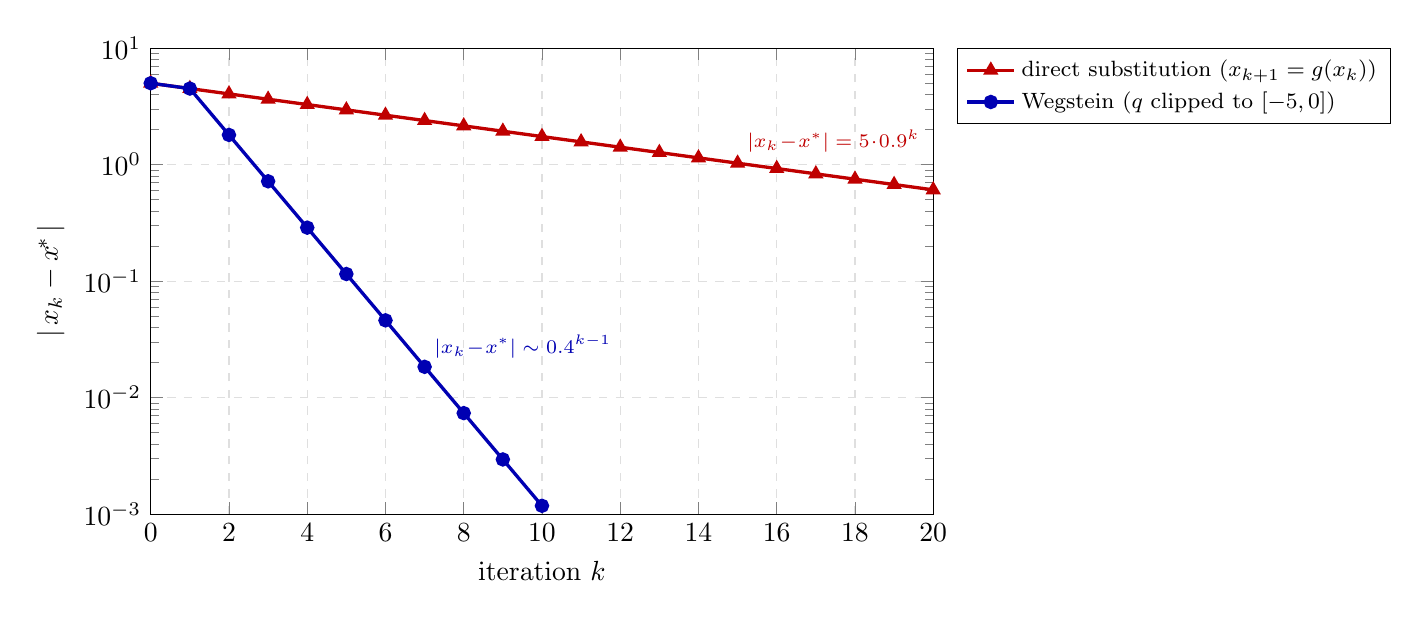
\begin{tikzpicture}
\begin{semilogyaxis}[
    width=0.95\linewidth, height=7.5cm,
    xlabel={iteration $k$},
    ylabel={$|\,x_k - x^{\!*}\,|$},
    xmin=0, xmax=20,
    ymin=1e-3, ymax=10,
    grid=major,
    grid style={gray!25, dashed},
    legend pos=outer north east,
    legend cell align=left,
    legend style={font=\footnotesize},
    every axis title/.style={below=1ex, at={(0.5,1)}, anchor=south},
]
% Direct substitution on g(x) = 0.9 x + 0.5, x* = 5.  Error_k = 5 * 0.9^k
% Computed exactly (geometric).
\addplot[red!75!black, very thick, mark=triangle*, mark size=2pt] coordinates {
    (0, 5.0000) (1, 4.5000) (2, 4.0500) (3, 3.6450) (4, 3.2805)
    (5, 2.9525) (6, 2.6572) (7, 2.3915) (8, 2.1524) (9, 1.9371)
    (10, 1.7434) (11, 1.5691) (12, 1.4122) (13, 1.2710) (14, 1.1439)
    (15, 1.0295) (16, 0.9265) (17, 0.8339) (18, 0.7505) (19, 0.6754)
    (20, 0.6079)
};
\addlegendentry{direct substitution ($x_{k+1} = g(x_k)$)}
% Wegstein on the same g(x) with q clipped to [-5, 0].
% For linear g(x) = ax + b, s_k = a always, q = a/(a-1) = 0.9/-0.1 = -9,
% clipped to -5.  Error contracts by |6a - 5| / 1 = |5.4 - 5| = 0.4 per step.
% Computed: x_0 = 0, x_1 = 0.5, then x_{k+1} = -5 x_k + 6 g(x_k).
\addplot[blue!70!black, very thick, mark=*, mark size=2pt] coordinates {
    (0, 5.0000) (1, 4.5000) (2, 1.8000) (3, 0.7200) (4, 0.2880)
    (5, 0.1152) (6, 0.0461) (7, 0.0184) (8, 0.00737) (9, 0.00295)
    (10, 0.00118)
};
\addlegendentry{Wegstein ($q$ clipped to $[-5,0]$)}
\node[anchor=south west, font=\scriptsize, text=blue!70!black]
    at (axis cs:7, 0.018) {$|x_k\!-\!x^*| \sim 0.4^{k-1}$};
\node[anchor=south west, font=\scriptsize, text=red!75!black]
    at (axis cs:15, 1.05) {$|x_k\!-\!x^*| = 5\!\cdot\! 0.9^{k}$};
\end{semilogyaxis}
\end{tikzpicture}
\caption{Wegstein vs.\ direct substitution on the test problem
$g(x)\!=\!0.9\,x\!+\!0.5$ with fixed point $x^*\!=\!5$ (chosen so that
$g'(x^*)\!=\!0.9$ is close to one --- direct substitution converges
slowly).  Direct substitution contracts at rate $0.9$ (geometric, dotted
red); Wegstein with $q$ clipped to $[-5,0]$ contracts at rate $\sim
0.4$, two-and-a-half times faster on a logarithmic scale.  After ten
iterations Wegstein has reduced the error by three orders of magnitude
where direct substitution has barely halved it; after twenty
iterations the gap is six orders.}
\label{fig:wegstein-vs-directsub}
\end{figure}

% ---------------------------------------------------------------------
\section{Closing a recycle: Newton on the tear stream}\label{ch:newton-tears}

\begin{whatyoulllearn}
A flowsheet with a recycle has a directed cycle: a downstream unit
feeds an upstream one, so no unit can be solved until the stream
entering the loop is already known --- a chicken-and-egg the simulator
breaks by \emph{tearing} the loop, guessing the torn stream, sweeping
once, and iterating until the guess reproduces itself.  The previous
chapter accelerated that iteration scalar-by-scalar with Wegstein.
This chapter takes the alternative the simulator now uses by default:
treat the whole torn stream as one vector and drive its residual to
zero with the $n$-dimensional Newton of Chapter~\ref{ch:nrND}.  We
derive the tear residual, justify the choice of tear variables, and
--- via a real bug the change exposed --- explain why the residual must
be \emph{relative}.
\end{whatyoulllearn}

\subsection{The recycle as a fixed-point in the tear stream}

Recall the tearing picture from Chapter~\ref{ch:sm-architecture}.  Cut
one stream in the cycle --- the \emph{tear stream} --- and let
$\mathbf{x}$ be its state (flows, temperature).  Guessing
$\mathbf{x}$ makes the loop acyclic: every unit now has a known inlet,
so one pass of the ordinary sequential-modular executive can be run,
unit by unit, all the way around the loop until it recomputes the torn
stream.  Call the result of that one full sweep
\begin{equation}
   \mathbf{x}^{\text{new}} \;=\; G(\mathbf{x}),
\end{equation}
where $G$ is ``run the whole flowsheet once, starting from this tear
guess''.  The recycle is converged when the guess reproduces itself,
\begin{equation}
   G(\mathbf{x}^{\!*}) \;=\; \mathbf{x}^{\!*}
   \qquad\Longleftrightarrow\qquad
   \mathbf{r}(\mathbf{x}^{\!*}) \;\equiv\; G(\mathbf{x}^{\!*}) - \mathbf{x}^{\!*} \;=\; \mathbf{0}.
   \label{eq:tear-residual}
\end{equation}
Wegstein attacks the left form (a fixed point $\mathbf{x} = G(\mathbf{x})$,
accelerated component-wise).  Newton attacks the right form (a root
$\mathbf{r}(\mathbf{x}) = \mathbf{0}$), all components at once.  Same
$G$, same sweep, same per-unit pedagogy --- only the outer iteration
differs.

% --- Figure: the recycle tear loop -----------------------------------
\begin{figure}[h]
\centering
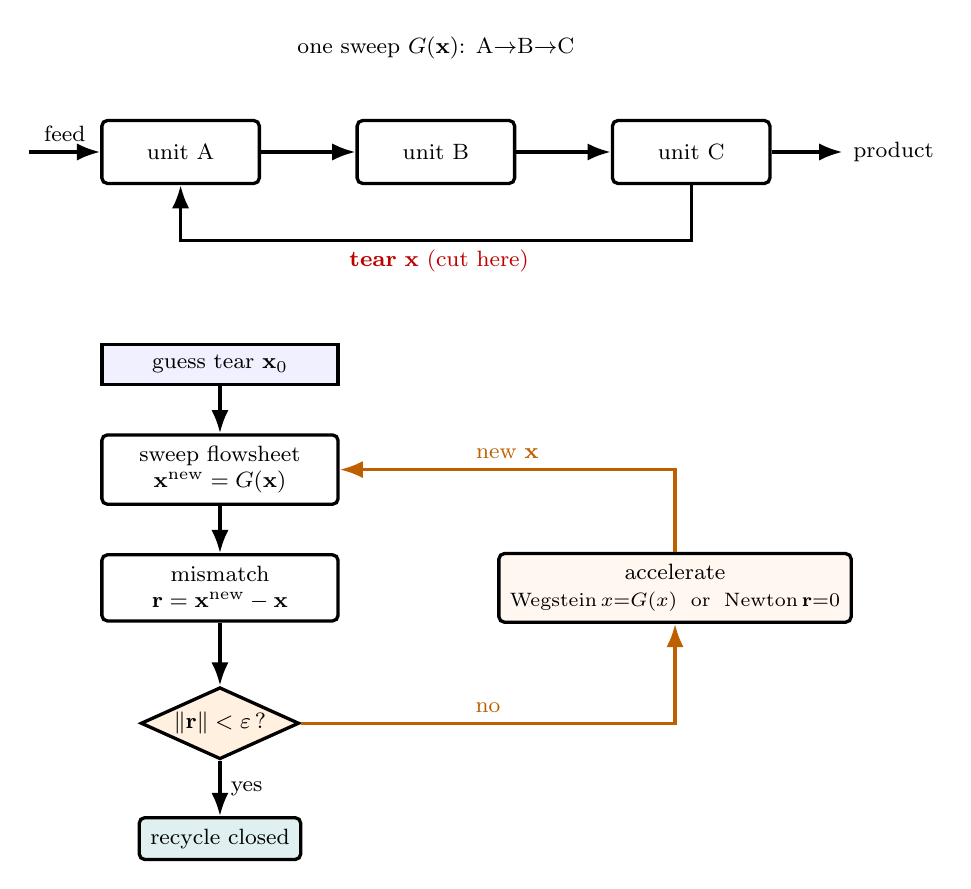
\begin{tikzpicture}[
    >={Latex[width=2.2mm]},
    every node/.style={font=\footnotesize},
    box/.style ={draw, rounded corners=2pt, very thick, align=center,
                 inner sep=4pt, minimum height=8mm, minimum width=20mm},
    io/.style  ={draw, very thick, fill=blue!6, align=center,
                 inner sep=4pt, minimum width=30mm},
    test/.style={draw, diamond, aspect=2.2, very thick, fill=orange!12,
                 align=center, inner sep=1pt},
    done/.style={draw, rounded corners=2pt, very thick, fill=teal!12,
                 align=center, inner sep=4pt},
    flow/.style={->, very thick},
    tear/.style={->, very thick, red!75!black, dashed},
    acc/.style ={->, very thick, orange!75!black},
]
% --- left: the physical flowsheet with one torn stream ---
\node[box] (u1) {unit A};
\node[box, right=12mm of u1] (u2) {unit B};
\node[box, right=12mm of u2] (u3) {unit C};
\draw[flow] ($(u1.west)+(-9mm,0)$) -- (u1.west) node[midway,above]{feed};
\draw[flow] (u1) -- (u2);
\draw[flow] (u2) -- (u3);
\draw[flow] (u3.east) -- ++(9mm,0) node[right]{product};
% recycle loop C -> A, with the TEAR scissor
\draw[flow] (u3.south) |- ($(u2.south)+(0,-7mm)$) -| (u1.south);
\node[red!75!black] at ($(u2.south)+(0,-7mm)$) [below] {\;\textbf{tear} $\xv$ (cut here)};
\node at ($(u2.north)+(0,9mm)$) {one sweep $G(\xv)$: A$\to$B$\to$C};

% --- right: the outer convergence loop ---
\node[io,   below=20mm of u1.south west, anchor=north west] (guess) {guess tear $\xv_0$};
\node[box,  below=6mm of guess, minimum width=30mm] (sweep) {sweep flowsheet\\$\xv^{\text{new}}=G(\xv)$};
\node[box,  below=6mm of sweep, minimum width=30mm] (mis)   {mismatch\\$\rv=\xv^{\text{new}}-\xv$};
\node[test, below=8mm of mis] (conv) {$\|\rv\|<\varepsilon$\,?};
\node[done, below=7mm of conv] (out) {recycle closed};
\node[box,  right=20mm of mis, minimum width=34mm, fill=orange!6] (acc)
     {accelerate\\{\scriptsize Wegstein\,$x{=}G(x)$ \;or\; Newton\,$\rv{=}0$}};
\draw[flow] (guess) -- (sweep);
\draw[flow] (sweep) -- (mis);
\draw[flow] (mis)   -- (conv);
\draw[flow] (conv)  -- node[right]{yes} (out);
\draw[acc]  (conv.east) -| node[pos=0.25,above]{no} (acc.south);
\draw[acc]  (acc.north) |- (sweep.east) node[pos=0.75,above]{new $\xv$};
\end{tikzpicture}
\caption{Closing a recycle.  \emph{Left:} the physical flowsheet has a
cycle (C feeds back to A); cutting the recycle at the dashed
\textbf{tear} turns it into an open chain whose one sweep
$G(\xv)=$ ``run A$\to$B$\to$C from this tear guess'' is just the
ordinary sequential pass.  \emph{Right:} the outer loop guesses the
tear, sweeps once, measures the mismatch $\rv=G(\xv)-\xv$, and --- if it
is still too large --- hands $\rv$ to an accelerator (Wegstein on the
fixed point, or Newton on the root) to propose a better tear, then
sweeps again.  The convergence is reached when the guess reproduces
itself.  Crucially, the per-unit physics inside $G$ never changes; only
the box that proposes the \emph{next} tear differs between Wegstein and
Newton.}
\label{fig:recycle-tear-loop}
\end{figure}

\subsection{What goes in the tear vector}

A process stream carries a total flow, a composition, a temperature,
a pressure and a phase split --- but these are not all independent, and
a good tear vector should use only independent coordinates.  The
tempting choice ``total flow $F$ plus all mole fractions $z_i$'' is
\emph{redundant}: the fractions obey $\sum_i z_i = 1$, so
$(F, z_1, \dots, z_{N_c})$ carries $N_c + 1$ numbers for a stream whose
physical content is only its $N_c$ component flows.  The redundancy is
not catastrophic --- it does \emph{not}, on its own, make the Jacobian
singular: the surplus direction (the one that holds every component
flow $F z_i$ fixed while trading $F$ off against the $z_i$) leaves $G$
unchanged, so $\partial G/\partial\mathbf{x}$ annihilates it and the
Jacobian $\Jac = \partial G/\partial\mathbf{x} - \mathbf{I}$ maps it to
the harmless eigenvalue $-1$, not $0$.  It is simply wasteful and
awkward: one extra variable (hence an extra pair of Jacobian sweeps),
and the iterate's $z_i$ must be re-normalised onto the simplex every
step or they drift and $F$ loses its meaning.

Choupo sidesteps this by tearing on \emph{component molar flows} plus
temperature,
\begin{equation}
   \mathbf{x} \;=\; (F_1,\, F_2,\, \dots,\, F_{N_c},\, T),
   \qquad F_i \equiv F z_i,
   \label{eq:tear-vars}
\end{equation}
which are mutually independent --- there is no normalisation tying them
together (the total $F = \sum_i F_i$ and the fractions $z_i = F_i/F$
are recovered afterwards).  Pressure and phase split are not torn:
pressure is set by the units, and the phase fractions follow from a
flash on the converged $(F_i, T)$.  For $N_c$ components the tear
vector has $N_c + 1$ entries.

\subsection{Newton on the tear residual}

With the residual \eqref{eq:tear-residual} in hand, the rest is the
machinery of Chapter~\ref{ch:nrND} applied verbatim.  The Jacobian
\begin{equation}
   \Jac \;=\; \frac{\partial \mathbf{r}}{\partial \mathbf{x}}
        \;=\; \frac{\partial G}{\partial \mathbf{x}} - \mathbf{I}
\end{equation}
is built by \emph{central} finite differences: perturb tear variable
$j$ by $\pm\delta$, run a full sweep $G$ at each, and the symmetric
difference $[\,G(\mathbf{x}+\delta\mathbf{e}_j) -
G(\mathbf{x}-\delta\mathbf{e}_j)\,]/2\delta$ gives column $j$.  That is
\emph{two} sweeps per variable, $2(N_c + 1)$ sweeps per Jacobian ---
the price Newton pays that Wegstein (one sweep per step) does not.
Central differences cost twice what forward ones would, but are
$O(\delta^2)$ accurate rather than $O(\delta)$, which keeps the
Jacobian --- and the convergence rate it drives --- clean.
Each Newton step then solves the linear system
\begin{equation}
   \Jac\, \Delta\mathbf{x} \;=\; -\,\mathbf{r}(\mathbf{x}),
\end{equation}
by the same Gauss elimination with partial pivoting, takes
$\mathbf{x} \leftarrow \mathbf{x} + \alpha\,\Delta\mathbf{x}$ under a
backtracking line search (start at $\alpha = 1$ and halve it until the
residual norm $\|\mathbf{r}\|$ actually drops, so the method stays
robust far from the solution), and repeats.  In code this is literally
a call to \code{solver::newtonND} with $\mathbf{r}$ as the residual
functor --- the recycle reuses the project's one general-purpose $n$-D
Newton, no special-case algebra.  Near the solution it converges
essentially \emph{quadratically} --- the number of correct digits
roughly doubles each step, the $O(\delta^2)$ central-difference
Jacobian holding that rate down to a very low floor --- where Wegstein
only improves super-linearly.

\subsection{Why the residual must be relative --- a bug story}

There is a subtlety that bites hard, and the simulator learned it the
painful way.  Write the convergence test naively as an
\emph{absolute} norm, $\|\mathbf{r}\| < \varepsilon$ with, say,
$\varepsilon = 10^{-5}$.  Now look at what is inside $\mathbf{r}$ for a
typical tear: a temperature near $365$ and component flows that, for a
small recycle, can be of order $2\times 10^{-4}$\,kmol/s.  The norm is
\emph{dominated by the temperature residual}.  A solver can satisfy
$\|\mathbf{r}\| < 10^{-5}$ with the temperature pinned to six digits
while the tiny tear flow is still off by 5\,\% --- and report success.

That is exactly what happened.  The \file{process03\_recycle} tutorial
ran for versions with its recycle flow converged to only a few
percent; the recorded golden value was itself under-converged, and
nobody noticed because the exit code was zero and the temperature
looked perfect.  The fix is to make every component of the residual
\emph{dimensionless and comparable} by scaling each by the magnitude
of its own variable:
\begin{equation}
   \boxed{\;
   \tilde r_i \;=\; \frac{G_i(\mathbf{x}) - x_i}{s_i},
   \qquad
   s_i = \begin{cases}
            F_{\text{tot}} & \text{for a component-flow entry},\\[2pt]
            T              & \text{for the temperature entry},
         \end{cases}
   \;}
   \label{eq:tear-relative}
\end{equation}
so that ``converged'' means \emph{every} variable --- the dominant
temperature and the faint trace flow alike --- has stopped moving to
the same relative precision.  With \eqref{eq:tear-relative} the
process03 recycle converges to its true fixed point
($F \approx 2.008\times 10^{-4}$\,kmol/s, $\|\tilde{\mathbf{r}}\|
\approx 5\times 10^{-9}$ in five Newton steps), and the golden master
was re-recorded against that genuinely-converged answer.

\begin{intuition}
A residual norm is only as trustworthy as its worst-scaled component.
Mixing a temperature ($\sim 10^{2}$) and a trace flow ($\sim 10^{-4}$)
in one absolute norm is like checking that a bridge is level by
averaging the height of the towers and the rivets --- the towers
swamp the average and a crooked rivet passes.  Scale first, then
compare.
\end{intuition}

\subsection{Wegstein or Newton? Choosing the recycle solver}

Both are available; \code{recycleSolver Newton;} is the default and

\begin{figure}[ht]
\centering
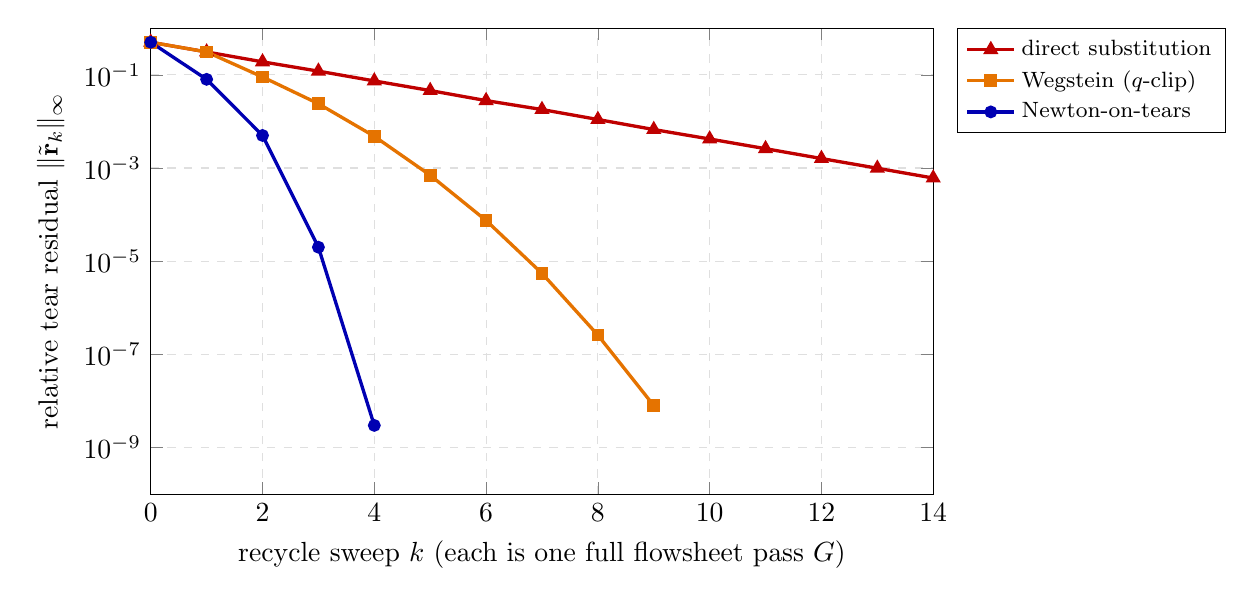
\begin{tikzpicture}
\begin{semilogyaxis}[
    width=0.95\linewidth, height=7.5cm,
    xlabel={recycle sweep $k$ (each is one full flowsheet pass $G$)},
    ylabel={relative tear residual $\|\tilde{\rv}_k\|_\infty$},
    xmin=0, xmax=14,
    ymin=1e-10, ymax=1,
    grid=major,
    grid style={gray!25, dashed},
    legend pos=outer north east,
    legend cell align=left,
    legend style={font=\footnotesize},
]
% Direct substitution: contraction factor ~0.62 on a tightly-coupled tear.
\addplot[red!75!black, very thick, mark=triangle*, mark size=2pt] coordinates {
    (0,5.0e-1)(1,3.1e-1)(2,1.9e-1)(3,1.2e-1)(4,7.4e-2)(5,4.6e-2)
    (6,2.8e-2)(7,1.8e-2)(8,1.1e-2)(9,6.7e-3)(10,4.2e-3)(11,2.6e-3)
    (12,1.6e-3)(13,9.9e-4)(14,6.1e-4)
};
\addlegendentry{direct substitution}
% Wegstein: super-linear, ~q-clipped.
\addplot[orange!90!black, very thick, mark=square*, mark size=1.7pt] coordinates {
    (0,5.0e-1)(1,3.1e-1)(2,9.0e-2)(3,2.4e-2)(4,4.8e-3)(5,7.0e-4)
    (6,7.5e-5)(7,5.5e-6)(8,2.6e-7)(9,8.0e-9)
};
\addlegendentry{Wegstein ($q$-clip)}
% Newton-on-tears: quadratic. Few sweeps per step but converges in ~5 outer.
\addplot[blue!70!black, very thick, mark=*, mark size=1.7pt] coordinates {
    (0,5.0e-1)(1,8.0e-2)(2,5.0e-3)(3,2.0e-5)(4,3.0e-9)
};
\addlegendentry{Newton-on-tears}
\end{semilogyaxis}
\end{tikzpicture}
\caption{The three ways to close the same coupled recycle, plotted as
relative tear residual versus outer sweep (\file{process03\_recycle}).
Direct substitution contracts at a fixed geometric rate --- a straight
line on the log scale, slow whenever the loop gain is near one.
Wegstein bends downward (super-linear: each step's reduction improves
as the secant sharpens), and Newton-on-tears dives quadratically,
clearing machine precision in $\sim\!5$ outer steps.  The catch hidden
by the $x$-axis: a Newton step costs $2(N_c{+}1)$ sweeps to build its
central-difference Jacobian, while Wegstein and direct substitution
cost one sweep each --- so Newton wins on \emph{coupled} tears where its
Jacobian pays for itself, and Wegstein wins when sweeps are dear and the
tear is nearly diagonal.}
\label{fig:tear-convergence-compare}
\end{figure}

\code{recycleSolver Wegstein;} keeps the accelerator.  They trade
off cleanly:

\begin{center}\small
\begin{tabular}{@{}p{0.30\linewidth}p{0.31\linewidth}p{0.31\linewidth}@{}}
\toprule
 & \textbf{Wegstein} & \textbf{Newton-on-tears} \\
\midrule
cost per outer step & one sweep & $2(N_c + 1)$ sweeps (central-difference Jacobian) \\
convergence & super-linear & quadratic \\
coupling between tear variables & ignored (component-wise scalars) & captured (full Jacobian) \\
robustness on counter-current / strongly-coupled tears & needs damping ($q$-clip) & strong \\
best when & loosely-coupled single tear & coupled and/or multiple tears \\
\bottomrule
\end{tabular}
\end{center}

Newton wins when the tear variables are coupled --- a change in one
component flow swings the others through the units --- because its
Jacobian sees that coupling, which Wegstein's independent scalars
cannot.  Wegstein can still be the better tool when sweeps are
expensive and the tear is nearly diagonal, or as a robust damped
fallback: the counter-current double-effect evaporator
\file{evaporator05} runs damped Wegstein ($q_{\min} = -0.7$) to tame
the over-shoot endemic to backward-feed vapour recycles, where an
undamped step would oscillate.

\subsection{This is not equation-oriented --- and that is the point}

It is tempting to call Newton-on-tears ``equation-oriented'', but it is
not.  A true equation-oriented (EO) solver collapses \emph{every}
unit's internal equations and \emph{every} stream connection into one
giant sparse system and Newtons on all of it at once; the units lose
their identity as solvable modules.  Choupo deliberately does not do
that (see the v1.0 note in \file{CLAUDE.md}): full EO needs hand-rolled
sparse linear algebra, and it dissolves the per-unit transparency that
is the whole pedagogical point --- a student can no longer watch a
single flash or reactor converge in isolation.

Newton-on-tears keeps the sequential-modular skeleton intact --- each
unit still solves itself, $G$ is still one honest sweep --- and wraps
\emph{only the recycle} in a Newton.  It is the Pareto step: most of
the convergence robustness of EO, at none of its architectural cost,
on the handful of variables (the tears) where the coupling actually
lives.  If the project ever adds a true EO mode it will be an opt-in
alternative (\code{solver eo;}) offered \emph{alongside} the modular
path, precisely so the manual can teach the contrast --- not a
replacement for it.

\begin{tutoriallink}
\file{tutorials/steady/flowsheets/process03\_recycle} --- reactor--separator with
a recycle, \code{recycleSolver Newton;} explicit; the genuinely-tight
fixed point of the bug story above.
\file{tutorials/steady/flowsheets/process05\_isomerization\_recycle} --- a second
Newton recycle.
\file{tutorials/steady/evaporation/evaporator05\_counter\_current} --- two tear
streams closed with damped \code{recycleSolver Wegstein;}, the
counter-current case where damping earns its keep.
\end{tutoriallink}

% ---------------------------------------------------------------------
\section{Direct search: Nelder-Mead}\label{ch:nelder-mead}

\begin{whatyoulllearn}
Newton and Levenberg-Marquardt need derivatives.  Wegstein needs a
fixed-point iteration.  When the objective is the output of a long,
discontinuous, or noisy simulator pass --- as it is whenever we ask
``what reflux ratio minimises the reboiler duty?'' --- derivatives may
not exist as smooth analytical objects, and finite differences may
amplify noise.  Nelder-Mead is the canonical \emph{derivative-free}
optimiser: it maintains a geometric simplex of $n+1$ points in $\mathbb
R^n$ and crawls downhill by reflecting and contracting that shape.  It
is the algorithm behind \texttt{outerDict type optimization}.
\end{whatyoulllearn}

\subsection*{The problem}

We want to minimise a scalar
\[
    f : \mathbb R^n \longrightarrow \mathbb R,
\]
where $f$ is provided as a black box --- evaluating $f(\xv)$ runs one
full simulator pass on a flowsheet with the design variables $\xv$
written into the dictionary, and (optionally) a post-processing chain
(sizing + costing) on top of the result.  We have:
\begin{itemize}
    \item no symbolic derivative;
    \item finite differences are expensive (each one is another full
          simulator pass) \emph{and} noisy when the inner solvers carry
          their own tolerance;
    \item bounds on each $x_i$ (refluxes cannot be negative, reactor
          volumes cannot exceed your budget).
\end{itemize}
The Nelder-Mead simplex algorithm \cite{NelderMead1965} sidesteps all
three obstacles.

\subsection*{The simplex}

A simplex in $\mathbb R^n$ is a set of $n+1$ vertices,
\[
    \mathcal S = \{\xv^{(0)}, \xv^{(1)}, \ldots, \xv^{(n)}\},
\]
in general position --- they span $\mathbb R^n$ as an affine basis.  In
two dimensions a simplex is a triangle; in three, a tetrahedron.  At
each iteration we order the vertices by their objective values:
\[
    f(\xv_{\mathrm{best}})
    \;\le\; f(\xv_{\mathrm{second}})
    \;\le\; \cdots
    \;\le\; f(\xv_{\mathrm{worst}}).
\]
We then try to replace the worst vertex by something better, leaving
the other $n$ alone.

\subsection*{The four moves}

Let $\xv_c$ be the centroid of all vertices \emph{except} the worst:

\begin{figure}[ht]
\centering
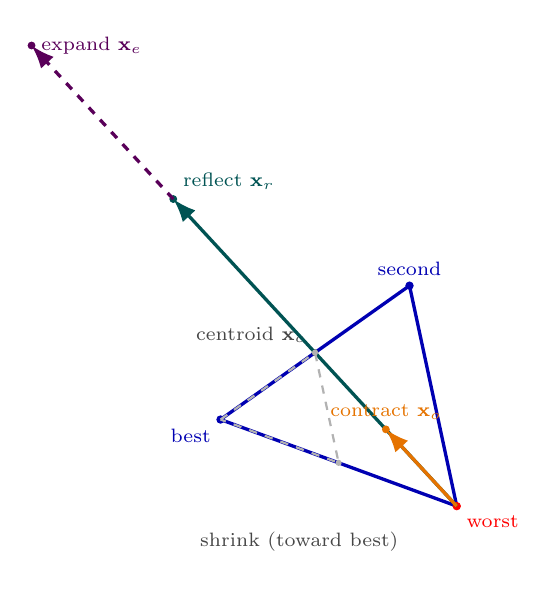
\begin{tikzpicture}[
    >={Latex[width=2.2mm]},
    every node/.style={font=\scriptsize},
    scale=1.0,
]
% base triangle: best B, second S, worst W ; centroid c of B,S
\coordinate (B) at (0,0);
\coordinate (S) at (2.4,1.7);
\coordinate (W) at (3.0,-1.1);
\coordinate (c) at ($(B)!0.5!(S)$);          % centroid of the two kept vertices
% reflected r = 2c - W
\coordinate (r) at ($2*(c) - 1*(W)$);
% expansion e = 2r - c
\coordinate (e) at ($2*(r) - 1*(c)$);
\coordinate (o) at ($(c)!0.5!(W)$);          % inside/outside contraction (toward centroid)
% the simplex
\draw[blue!70!black, very thick] (B) -- (S) -- (W) -- cycle;
\filldraw[blue!70!black] (B) circle (1.3pt) node[below left] {best};
\filldraw[blue!70!black] (S) circle (1.3pt) node[above] {second};
\filldraw[red] (W) circle (1.3pt) node[below right] {worst};
\filldraw[gray!55!black] (c) circle (1.0pt) node[above left] {centroid $\xv_c$};
% reflection
\draw[->, teal!65!black, very thick] (W) -- (r);
\filldraw[teal!65!black] (r) circle (1.2pt) node[above right] {reflect $\xv_r$};
% expansion (further along)
\draw[->, violet!70!black, very thick, dashed] (r) -- (e);
\filldraw[violet!70!black] (e) circle (1.2pt) node[right] {expand $\xv_e$};
% contraction (toward centroid)
\filldraw[orange!90!black] (o) circle (1.2pt) node[above] {contract $\xv_o$};
\draw[->, orange!90!black, very thick] (W) -- (o);
% shrink: pull S and W halfway to B (faint)
\coordinate (Sh) at ($(B)!0.5!(S)$);
\coordinate (Wh) at ($(B)!0.5!(W)$);
\draw[gray!60, thick, dashed] (B) -- (Sh) -- (Wh) -- cycle;
\filldraw[gray!60] (Sh) circle (0.9pt);
\filldraw[gray!60] (Wh) circle (0.9pt);
\node[gray!55!black] at (1.0,-1.55) {shrink (toward best)};
\end{tikzpicture}
\caption{The four Nelder--Mead moves as geometry, on a triangular
simplex ($n=2$).  All candidates lie on the line through the worst
vertex and the centroid $\xv_c$ of the kept vertices.  \emph{Reflection}
(teal) flips the worst point through $\xv_c$; if that is wildly
successful, \emph{expansion} (violet, dashed) pushes further along the
same ray; if reflection lands on a hill, \emph{contraction} (orange)
pulls back toward $\xv_c$; and if even that fails, \emph{shrink} (grey,
dashed) drags every vertex but the best halfway in, making the whole
simplex smaller and more local.  Only shrink re-evaluates more than one
vertex --- it is the algorithm conceding the reflection ray has stalled.
The decision tree of Fig.~\ref{fig:nelder-mead-tree} is exactly the rule
for picking which of these four points to keep.}
\label{fig:nelder-mead-moves}
\end{figure}

\[
    \xv_c \;=\; \frac{1}{n}\sum_{k \neq \mathrm{worst}} \xv^{(k)}.
\]
The candidates are formed along the line from the worst point through
the centroid.  In order of cost (each move is one extra evaluation):

\paragraph{1.\ Reflection.}
\[
    \xv_r \;=\; \xv_c + \alpha\,(\xv_c - \xv_{\mathrm{worst}}),
    \qquad \alpha = 1.
\]
The worst vertex is reflected through the centroid.  If $f(\xv_r)$
falls between $f(\xv_{\mathrm{best}})$ and $f(\xv_{\mathrm{second}})$,
the reflection is accepted and the iteration ends.

\paragraph{2.\ Expansion.}
If $f(\xv_r) < f(\xv_{\mathrm{best}})$, the reflection direction looks
\emph{very} promising; we extend further:
\[
    \xv_e \;=\; \xv_c + \gamma\,(\xv_r - \xv_c),
    \qquad \gamma = 2.
\]
Whichever of $\xv_e, \xv_r$ has the lower $f$ replaces the worst
vertex.

\paragraph{3.\ Contraction.}
If $f(\xv_r) \ge f(\xv_{\mathrm{second}})$, the reflection landed on a
hill; we shrink toward the centroid instead:
\[
    \xv_o \;=\; \xv_c + \rho\,(\xv_{\mathrm{worst}} - \xv_c),
    \qquad \rho = 0.5.
\]
(In Choupo we use \emph{outside contraction} ---
$\xv_c + \rho\,(\xv_r - \xv_c)$ --- when $f(\xv_r) < f(\xv_{\mathrm{worst}})$,
otherwise the inside form above.  Either way the new point is on the
line through $\xv_c$, closer to it.)

\paragraph{4.\ Shrink.}
If contraction also fails, every vertex except the best is pulled
halfway toward the best:
\[
    \xv^{(k)} \;\leftarrow\;
    \xv_{\mathrm{best}} + \sigma\,(\xv^{(k)} - \xv_{\mathrm{best}}),
    \qquad \sigma = 0.5,
\]
for $k \ne \mathrm{best}$.  This is the only move that re-evaluates
multiple vertices.  It is the algorithm's confession that progress
along the reflection line has stalled and the simplex needs to become
smaller and more local.

% --- Figure: the Nelder-Mead move decision tree ----------------------
\begin{figure}[h]
\centering
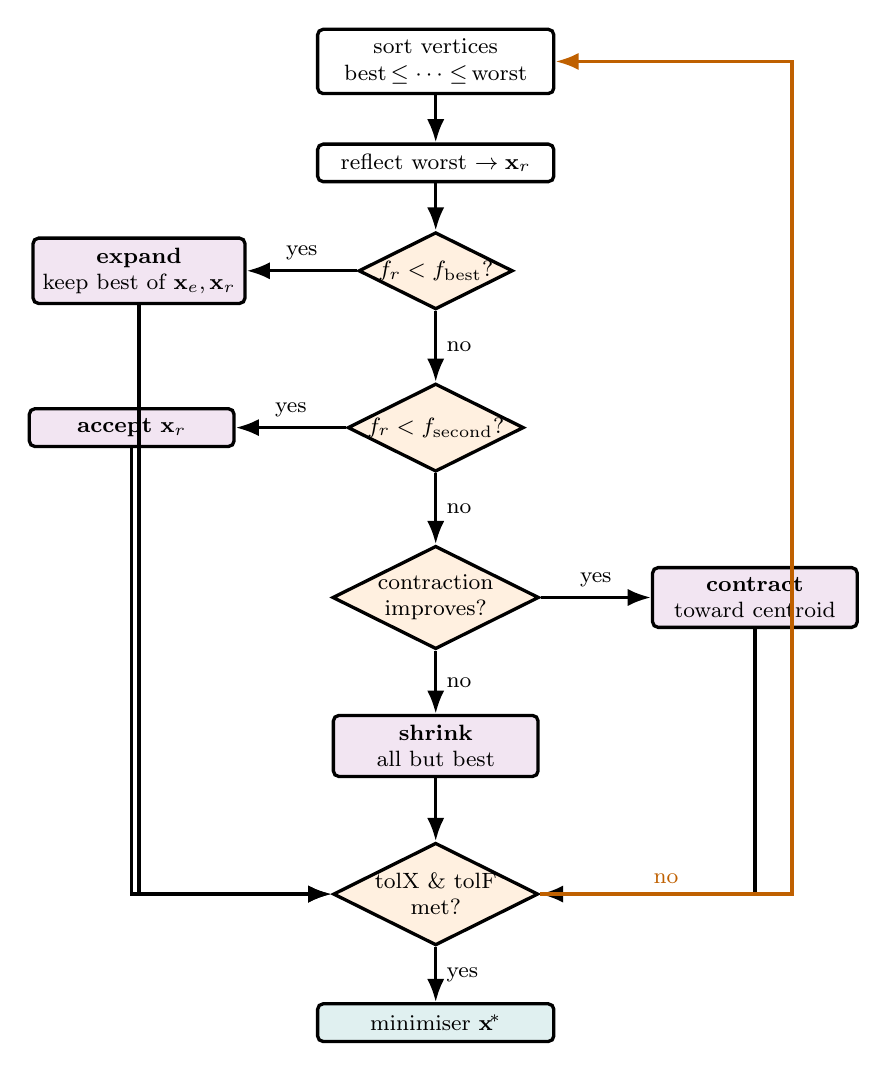
\begin{tikzpicture}[
    >={Latex[width=2.2mm]},
    every node/.style={font=\footnotesize},
    box/.style ={draw, rounded corners=2pt, very thick, align=center,
                 inner sep=3.5pt, minimum width=30mm},
    test/.style={draw, diamond, aspect=2.0, very thick, fill=orange!12,
                 align=center, inner sep=0pt},
    move/.style={draw, rounded corners=2pt, very thick, align=center,
                 inner sep=3.5pt, fill=violet!10, minimum width=26mm},
    done/.style={draw, rounded corners=2pt, very thick, fill=teal!12,
                 align=center, inner sep=4pt, minimum width=30mm},
    flow/.style={->, very thick},
    loop/.style={->, very thick, orange!75!black},
]
\node[box]  (sort) {sort vertices\\ best\,$\le\dots\le$\,worst};
\node[box,  below=6mm of sort]  (refl) {reflect worst $\to \xv_r$};
\node[test, below=6mm of refl]  (t1)   {$f_r<f_{\text{best}}$?};
\node[move, left=14mm of t1]     (exp)  {\textbf{expand}\\ keep best of $\xv_e,\xv_r$};
\node[test, below=9mm of t1]    (t2)   {$f_r<f_{\text{second}}$?};
\node[move, left=14mm of t2]     (acc)  {\textbf{accept} $\xv_r$};
\node[test, below=9mm of t2]    (t3)   {contraction\\ improves?};
\node[move, right=14mm of t3]    (con)  {\textbf{contract}\\ toward centroid};
\node[move, below=8mm of t3]     (shr)  {\textbf{shrink}\\ all but best};
\node[test, below=8mm of shr]   (conv) {tolX \& tolF\\ met?};
\node[done, below=7mm of conv]   (out)  {minimiser $\xv^{\!*}$};
\draw[flow] (sort) -- (refl);
\draw[flow] (refl) -- (t1);
\draw[flow] (t1) -- node[above]{yes} (exp);
\draw[flow] (t1) -- node[right]{no}  (t2);
\draw[flow] (t2) -- node[above]{yes} (acc);
\draw[flow] (t2) -- node[right]{no}  (t3);
\draw[flow] (t3) -- node[above]{yes} (con);
\draw[flow] (t3) -- node[right]{no}  (shr);
\draw[flow] (shr) -- (conv);
\draw[flow] (conv) -- node[right]{yes} (out);
% the accepted-move arrows all funnel into the convergence test
\draw[flow] (exp.south) |- (conv.west);
\draw[flow] (acc.south) |- (conv.west);
\draw[flow] (con.south) |- (conv.east);
% loop back if not converged
\draw[loop] (conv.east) -- ++(3.2,0) node[midway,above]{no} |- (sort.east);
\end{tikzpicture}
\caption{The Nelder--Mead move decision tree --- a derivative-free
descent that needs only $f$ values, used in Choupo wherever a Jacobian
is treacherous: the \emph{direct} Gibbs-energy minimisation of an LL or
VLL flash (\S\ref{ch:lle-gibbs}), and parameter-fitting in
\code{OptimizationDriver}.  Each pass orders the $n{+}1$ vertices,
reflects the worst through the centroid, and then --- by a short
cascade of cheap tests on the reflected value --- chooses the
\emph{expand} / \emph{accept} / \emph{contract} / \emph{shrink} move,
each just a point on the line through the centroid.  Only \emph{shrink}
re-evaluates several vertices; it is the algorithm conceding the
reflection line has stalled.  The simplex crawls downhill until it is
both small (tolX) and flat (tolF).  For the symmetric $\gamma$-models
where a Newton flash would collapse onto the trivial $K=1$ saddle, this
``crawl the Gibbs surface'' search --- multi-started --- is what finds
the true two-phase split.}
\label{fig:nelder-mead-tree}
\end{figure}

\subsection*{Box bounds without changing the algorithm}

Nelder-Mead is, by construction, unconstrained.  When the user supplies
bounds $\xv \in [\mathbf{x}_{\mathrm{lo}}, \mathbf{x}_{\mathrm{hi}}]$ for each variable, Choupo \emph{clips}
every candidate vertex back into the box element-wise \emph{before}
calling $f$:
\[
    x_i \;\leftarrow\; \min(\max(x_i, \mathrm{lo}_i), \mathrm{hi}_i).
\]
The simplex learns very quickly that probing the violation region pays
the same as the wall, so it contracts away from the wall.  This is the
simplest defensible handling; if you want a smooth penalty term or a
true active-set strategy, that is the job of an SQP or interior-point
wrapper, not Nelder-Mead.

\subsection*{Stopping criteria}

Two natural tests:
\begin{itemize}
    \item \textbf{tolX} --- the simplex has shrunk.  We compute the
          maximum coordinate-wise extent of the simplex, normalised
          \emph{per axis} by that axis's bound width:
          \[
              \mathrm{tolX\ trip} \;:\;
              \max_i \;
              \frac{\max_k |x^{(k)}_i - x^{\mathrm{best}}_i|}
                   {\mathrm{hi}_i - \mathrm{lo}_i}
              \;<\; \mathrm{tolX}.
          \]
          The per-axis normalisation is crucial: if one variable is a
          reactor volume in $\mathrm{m^3}$ and the other a temperature
          in K, a global $\|\Delta \xv\|$ would be dominated by the
          larger scale and would stop the algorithm before the small
          axis has converged.  Choupo uses this scaled criterion.
    \item \textbf{tolF} --- the range of $f$ over the simplex is small
          relative to $|f_{\mathrm{best}}|$.  Useful when $f$ is flat
          near the optimum.
\end{itemize}
Plus the usual safety net of \texttt{maxIter}.

\subsection*{When Nelder-Mead is the right hammer}

\begin{itemize}
    \item Modest number of design variables (say $n \le 10$).  The
          simplex needs $n+1$ vertices and each iteration costs at
          least one new evaluation, so the wall-clock cost grows
          gracefully in $n$.
    \item Black-box, possibly noisy, possibly discontinuous objective.
          The simulator pass is exactly that.
    \item Local search.  Nelder-Mead converges to a local minimum near
          the initial simplex; for a global search you would restart
          with several random simplexes (\emph{multi-start}) and keep
          the best.
\end{itemize}

\subsection*{When to reach for something else}

\begin{itemize}
    \item High dimension ($n \gg 10$).  Simplex moves become inefficient
          because each move only affects one vertex; on a 50-D problem,
          a quasi-Newton method with finite differences typically wins
          despite the gradient cost.
    \item Smooth, differentiable objective with cheap derivatives.  Use
          a Newton-family method directly (Choupo's NewtonND, or LM
          for least-squares, both already in §\ref{ch:nrND} and
          §\ref{ch:lm}).
    \item Hard constraints, especially non-linear ones.  Use SQP ---
          Choupo's constrained optimiser, §\ref{ch:sqp} --- or an
          interior-point wrapper (Choupo offers no interior-point method).
\end{itemize}

\subsection*{What you see in Choupo}

The \texttt{OptimizationDriver} prints one line per simplex iteration,
showing the move type (\texttt{reflect} / \texttt{expand} /
\texttt{contract} / \texttt{shrink}), the current best $f$ value, the
current best $\xv$, and the simplex size.  Identical rows go into
\texttt{optimization\_history.csv} so the student can plot the
convergence trajectory.  On termination the simulator is replayed once
at the optimum with full verbosity, so the case directory ends with
the converged final state on standard output --- exactly as a direct
(non-outer) run would leave it.

% ---------------------------------------------------------------------
\section{Constrained optimisation: line-search SQP}\label{ch:sqp}

\begin{whatyoulllearn}
Nelder-Mead minimises a black box but cannot honour a hard constraint.
Sequential Quadratic Programming (SQP) does: at every iterate it
linearises the constraints, builds a convex \emph{quadratic} model of
the Lagrangian, solves that quadratic program (QP) for a step, then
shortens the step with an $\ell_1$ merit function until it makes
honest progress. We derive the QP from the KKT conditions, the
damped-BFGS curvature update that keeps the QP convex, the merit
function that arbitrates objective against feasibility, the Armijo
backtracking line search, and the five-residual KKT certificate
Choupo prints at the optimum. The inner convex QP is solved by an
active-set method, derived in §\ref{ch:active-set-qp}.
\end{whatyoulllearn}

The flowsheet optimiser often comes with real constraints: a purity
that must be \emph{at least} $0.99$, a duty that must \emph{equal} a
target, a recovery bounded above. Nelder-Mead (§\ref{ch:nelder-mead})
cannot see any of these --- it only ranks objective values, so a
constraint can only enter as a hand-tuned penalty, which distorts the
objective and is brittle. SQP \cite{NocedalWright,Powell1978} is the
classical answer: it treats the constraints as first-class citizens
and converges to a point that provably satisfies the Karush--Kuhn--Tucker
(KKT) optimality conditions. Choupo's \code{solver::sqp} is a
hand-rolled, finite-difference, line-search SQP --- no external library,
every quantity inspectable.

\subsection{The problem and the KKT conditions}

The general nonlinear program (NLP) Choupo's SQP solves is
\begin{equation}
   \min_{\xv \in \R^n} \; f(\xv)
   \quad \text{s.t.} \quad
   \begin{cases}
     h_j(\xv) = 0, & j = 1,\dots,m_{\mathrm e}, \\
     g_k(\xv) \le 0, & k = 1,\dots,m_{\mathrm i}, \\
     \mathrm{lo} \le \xv \le \mathrm{hi}, &
   \end{cases}
   \label{eq:sqp-nlp}
\end{equation}
with equalities $h_j$ (e.g.\ a DesignSpec residual), inequalities $g_k$
(written in the $\le 0$ convention --- a purity floor
$x_{\mathrm{purity}} \ge 0.99$ becomes $g = 0.99 - x_{\mathrm{purity}}
\le 0$), and box bounds. The Lagrangian collects every constraint with
a multiplier:
\begin{equation}
   \mathcal L(\xv, \boldsymbol\lambda, \boldsymbol\mu)
   \;=\; f(\xv)
   \;+\; \sum_{j} \lambda_j\, h_j(\xv)
   \;+\; \sum_{k} \mu_k\, g_k(\xv).
   \label{eq:sqp-lagrangian}
\end{equation}
A point $\xv^\star$ is a (first-order) constrained minimiser when the
\textbf{KKT conditions} hold:
\begin{align}
   \nabla_{\!\xv} \mathcal L
     &= \nabla f + \textstyle\sum_j \lambda_j \nabla h_j
        + \sum_k \mu_k \nabla g_k = \mathbf 0
     && \text{(stationarity)}, \label{eq:kkt-stat}\\
   h_j(\xv^\star) &= 0,\quad g_k(\xv^\star) \le 0
     && \text{(primal feasibility)}, \label{eq:kkt-feas}\\
   \mu_k &\ge 0
     && \text{(dual feasibility)}, \label{eq:kkt-dual}\\
   \mu_k\, g_k(\xv^\star) &= 0
     && \text{(complementary slackness)}. \label{eq:kkt-compl}
\end{align}
Complementarity \eqref{eq:kkt-compl} says: a constraint that is not

\begin{figure}[ht]
\centering
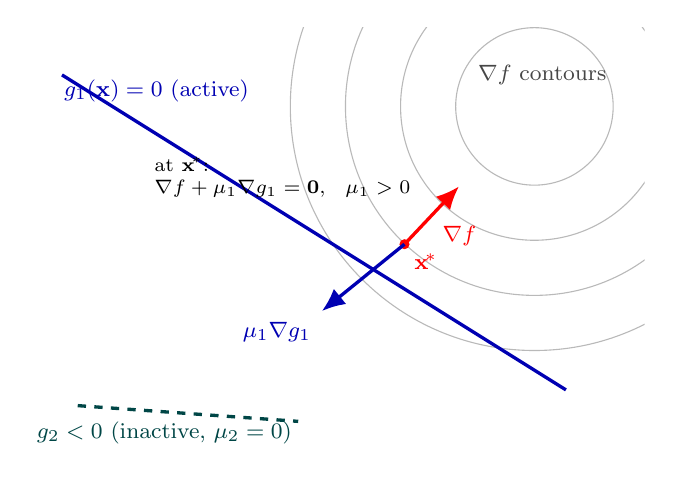
\begin{tikzpicture}[
    >={Latex[width=2.5mm]},
    every node/.style={font=\footnotesize},
    scale=1.0,
]
% feasible region: below an active constraint g1 (line) and bounded by box.
\begin{scope}
\clip (-0.1,-0.1) rectangle (7.6,5.2);
% objective contours (circles centred at unconstrained min, outside feasible)
\foreach \r in {1.0,1.7,2.4,3.1} {
   \draw[gray!55] (6.2,4.2) circle (\r);
}
\end{scope}
\node[gray!55!black] at (6.3,4.6) {$\nabla f$ contours};
% feasible region boundary: active inequality g1 (a line), feasible side below-left
\draw[blue!70!black, very thick] (0.2,4.6) -- (6.6,0.6);
\node[blue!70!black] at (1.4,4.4) {$g_1(\xv)=0$ (active)};
% an inactive inequality g2 (far away)
\draw[teal!55!black, very thick, dashed] (0.4,0.4) -- (3.2,0.2);
\node[teal!55!black] at (1.5,0.05) {$g_2<0$ (inactive, $\mu_2=0$)};
% constrained minimiser x* on g1, where a contour is tangent to g1
\coordinate (xs) at (4.55,2.45);
\filldraw[red] (xs) circle (1.6pt) node[below right]{$\xv^{\!*}$};
% gradient of f at x* (points toward higher f, away from contour centre)
\draw[->, red, very thick] (xs) -- ($(xs)!0.42!(6.2,4.2)$)
   node[midway, below right, text=red]{$\nabla f$};
% gradient of g1 (push), stationarity nabla f + mu nabla g1 = 0
\draw[->, blue!70!black, very thick] (xs) -- ($(xs)+(-1.05,-0.85)$)
   node[below left, text=blue!70!black]{$\mu_1\nabla g_1$};
% small note
\node[align=left, font=\scriptsize] at (3.0,3.3)
   {at $\xv^{\!*}$:\\ $\nabla f + \mu_1\nabla g_1 = \mathbf 0$,\;\; $\mu_1>0$};
\end{tikzpicture}
\caption{The KKT stationarity condition as a force balance at a
constrained minimiser.  The grey arcs are level sets of the objective
$f$; absent constraints, $f$ would keep decreasing toward its
unconstrained minimum (upper right).  The active inequality $g_1=0$
(blue line) blocks the way, so the constrained optimum $\xv^{\!*}$ sits
\emph{on} that boundary, where an objective contour is tangent to it.
There the objective gradient $\nabla f$ (red, pointing uphill) is
exactly cancelled by the constraint's push $\mu_1\nabla g_1$ (blue) ---
stationarity $\nabla f+\mu_1\nabla g_1=\mathbf 0$ with multiplier
$\mu_1>0$.  The second constraint $g_2$ (dashed teal) is slack: it does
not touch $\xv^{\!*}$, so by complementary slackness its multiplier is
zero and it exerts no force.  The active multiplier $\mu_1$ is the
\emph{shadow price} --- how much $f$ would improve per unit of relaxing
$g_1$ --- which is why Choupo prints it.}
\label{fig:kkt-geometry}
\end{figure}

binding ($g_k < 0$) carries no multiplier ($\mu_k = 0$); only
\emph{active} constraints ($g_k = 0$) can push back with $\mu_k > 0$.

\subsection{Shadow prices: what the multiplier is worth}\label{sec:sqp-shadow}

The multipliers are not bookkeeping --- they answer the question a
process engineer actually asks: \emph{``what is this constraint costing
me, and what would I pay to loosen it?''}  Perturb the right-hand side
of an active inequality, $g_k(\xv)\le b_k$, by a small $\Delta b_k$.  The
feasible set opens up, the optimum slides along the relaxed boundary,
and --- because at the optimum $\nabla_{\!\xv}\mathcal L=\mathbf 0$, so
only the \emph{explicit} dependence on $b_k$ survives (the envelope /
sensitivity theorem) --- the optimal objective moves by
\begin{equation}
   \frac{\partial f^\star}{\partial b_k} \;=\; -\,\mu_k
   \qquad\Longleftrightarrow\qquad
   \Delta f^\star \;\approx\; -\,\mu_k\,\Delta b_k .
   \label{eq:sensitivity}
\end{equation}
That is the whole reason the multiplier is called a \textbf{shadow
price}.  Read it economically --- with the sign flipped for a
\emph{maximisation}, since Choupo maximises NPV by minimising $-$NPV ---
and $\mu_k$ is the \textbf{marginal \texteuro{} value of one more unit of the
capped resource}: one more m\textsuperscript{3} of reactor, one more
\texteuro{} of capital budget, one more kg/h of market demand.  A binding
capital budget with $\mu=0.8$ says the next euro of CAPEX would buy
\texteuro{}0.80 of extra NPV (build it); a binding cap with $\mu=0.05$ is
barely worth relaxing; a \emph{slack} constraint has $\mu=0$ and can be
ignored entirely.  This is why \code{solver::sqp} prints the active set
and its multipliers every iteration and again in the closing KKT
certificate --- the shadow prices \emph{are} the design answer, not a
diagnostic.  The tutorial
\file{tutorials/steady/optimisation/optim05\_economic\_design}
maximises a small plant's NPV against a capital budget and a capacity
cap and reads the binding cap's shadow price straight off the
certificate.

\begin{figure}[ht]
\centering
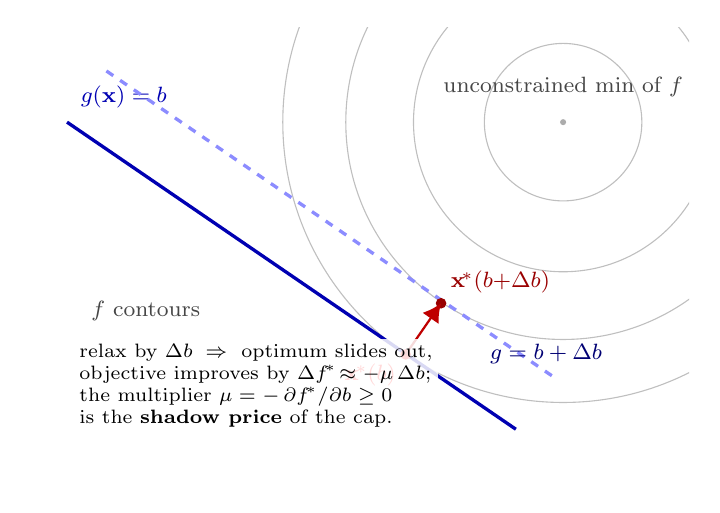
\begin{tikzpicture}[
    >={Latex[width=2.5mm]},
    every node/.style={font=\footnotesize},
    scale=1.0,
]
\begin{scope}
\clip (-0.2,-0.2) rectangle (8.2,5.6);
% objective contours: concentric circles around the unconstrained optimum
% (upper right, OUTSIDE the feasible set).  The two outer arcs are the ones
% the constrained optima sit on, so relaxing visibly moves to a smaller f.
\foreach \r in {1.0,1.9,2.76,3.56} {
   \draw[gray!50] (6.6,4.4) circle (\r);
}
\end{scope}
\fill[gray!65] (6.6,4.4) circle (1.1pt);
\node[gray!55!black, anchor=south] at (6.6,4.6) {unconstrained min of $f$};
\node[gray!55!black] at (1.3,2.0) {$f$ contours};
% original active constraint g = b (feasible side: lower-left)
\draw[blue!70!black, very thick] (0.3,4.4) -- (6.0,0.5);
\node[blue!70!black, anchor=south west] at (0.35,4.45) {$g(\xv)=b$};
% relaxed constraint g = b + db, parallel, shifted toward the unconstrained min
\draw[blue!45, very thick, dashed] (0.8,5.05) -- (6.5,1.15);
\node[blue!45!black, anchor=west] at (5.55,1.45) {$g=b+\Delta b$};
% constrained optimum on g=b (tangent to the outer contour r=3.56)
\coordinate (xb) at (4.6,1.45);
\filldraw[red] (xb) circle (1.7pt) node[below left]{$\xv^{\!*}(b)$};
% constrained optimum on the relaxed boundary (tangent to r=2.76, smaller f)
\coordinate (xbr) at (5.05,2.10);
\filldraw[red!60!black] (xbr) circle (1.7pt) node[above right]{$\xv^{\!*}(b{+}\Delta b)$};
% the optimum slides outward toward the unconstrained min
\draw[->, red!75!black, thick] (xb) -- (xbr);
% improvement callout
\node[align=left, font=\scriptsize, fill=white, fill opacity=0.85,
      text opacity=1, inner sep=2pt] at (2.7,1.05)
   {relax by $\Delta b\;\Rightarrow\;$ optimum slides out,\\
    objective improves by $\Delta f^{\!*}\!\approx-\mu\,\Delta b$;\\
    the multiplier $\mu=-\,\partial f^{\!*}/\partial b\ge 0$\\
    is the \textbf{shadow price} of the cap.};
\end{tikzpicture}
\caption{The multiplier as a price.  Contours of the objective $f$
(grey) tighten toward its unconstrained minimum (upper right), which the
active cap $g=b$ (solid blue) keeps out of reach, so the constrained
optimum $\xv^{\!*}(b)$ sits on that boundary, tangent to the outer
contour.  Loosen the cap to $g=b+\Delta b$ (dashed) and the boundary
shifts toward the unconstrained minimum; the optimum slides to
$\xv^{\!*}(b{+}\Delta b)$ on a \emph{smaller} contour --- a better
objective.  The rate of that improvement per unit of relaxation is
exactly the Lagrange multiplier, $\Delta f^{\!*}\approx-\mu\,\Delta b$
(Eq.~\ref{eq:sensitivity}): $\mu$ is the shadow price.  A constraint
that does not touch the optimum is slack, its multiplier is zero, and
moving it changes nothing --- complementary slackness, seen
geometrically.}
\label{fig:shadow-price}
\end{figure}

The multipliers are \emph{shadow prices} --- $\lambda_j$ (or $\mu_k$ for
an inequality) is the marginal change in the optimal $f$ per unit
relaxation of its constraint --- which is exactly the sensitivity a
process engineer wants, so Choupo prints them every iteration.

\subsection{From KKT to a quadratic program}

Newton's method on the nonlinear KKT system
\eqref{eq:kkt-stat}--\eqref{eq:kkt-feas} is the heart of SQP. Linearise
the constraints about the current $\xv$ and replace the Lagrangian by a
quadratic model in the step $\dv = \xv_{+} - \xv$, with curvature
matrix $\Bv \approx \nabla^2_{\!\xv\xv}\mathcal L$ (note: the Hessian of
the \emph{Lagrangian}, not of $f$ --- this is the single most common
SQP mistake; see §\ref{sec:sqp-bfgs}). The step solves the convex QP
\begin{equation}
   \min_{\dv \in \R^n} \;
     \tfrac12\, \dv^{\!\top} \Bv\, \dv + \nabla f^{\!\top} \dv
   \quad \text{s.t.} \quad
   \begin{cases}
     \nabla h_j^{\!\top} \dv + h_j = 0, \\
     \nabla g_k^{\!\top} \dv + g_k \le 0, \\
     \mathrm{lo} - \xv \le \dv \le \mathrm{hi} - \xv.
   \end{cases}
   \label{eq:sqp-qp}
\end{equation}
The constant $f(\xv)$ is dropped (it does not move the minimiser). The
linear-in-$\dv$ constraint rows are precisely the first-order Taylor
predictions $h_j(\xv + \dv) \approx h_j + \nabla h_j^{\!\top}\dv$ driven
to feasibility. The QP multipliers returned for

\begin{figure}[ht]
\centering
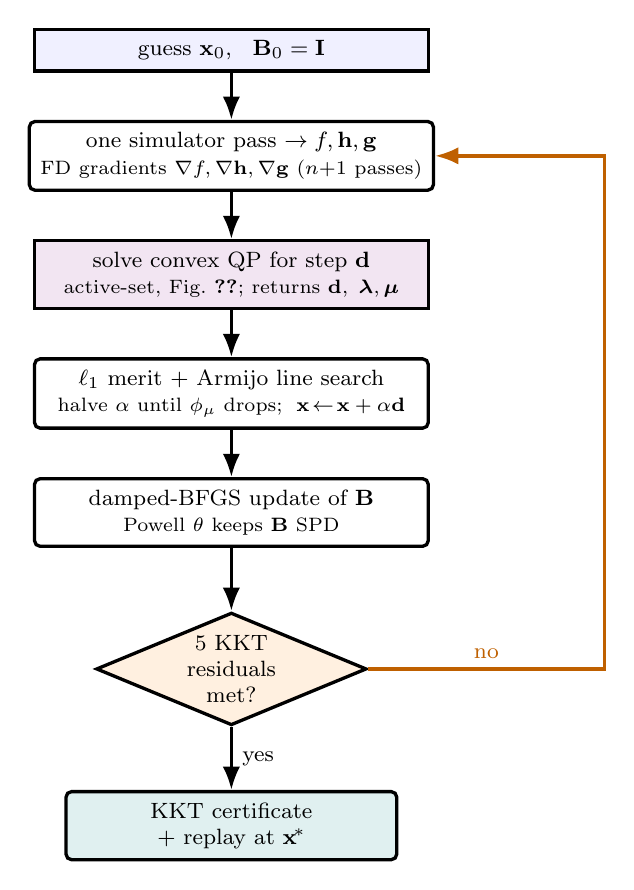
\begin{tikzpicture}[
    >={Latex[width=2.2mm]},
    every node/.style={font=\footnotesize},
    node distance = 6mm and 12mm,
    box/.style  ={draw, rounded corners=2pt, very thick, align=center,
                  inner sep=4pt, minimum width=50mm},
    io/.style   ={draw, very thick, fill=blue!6, align=center,
                  inner sep=4pt, minimum width=50mm},
    qp/.style   ={draw, very thick, fill=violet!10, align=center,
                  inner sep=4pt, minimum width=50mm},
    test/.style ={draw, diamond, aspect=2.4, very thick, fill=orange!12,
                  align=center, inner sep=1pt},
    done/.style ={draw, rounded corners=2pt, very thick, fill=teal!12,
                  align=center, inner sep=4pt, minimum width=42mm},
    flow/.style ={->, very thick},
    loop/.style ={->, very thick, orange!75!black},
]
\node[io]  (init) {guess $\xv_0$,\;\; $\Bv_0=\mathbf I$};
\node[box, below=of init] (fd)
   {one simulator pass $\to f,\mathbf h,\mathbf g$\\
    {\scriptsize FD gradients $\nabla f,\nabla\mathbf h,\nabla\mathbf g$ ($n{+}1$ passes)}};
\node[qp, below=of fd] (qp)
   {solve convex QP for step $\dv$\\
    {\scriptsize active-set, Fig.~\ref{fig:active-set-qp}; returns $\dv,\;\boldsymbol\lambda,\boldsymbol\mu$}};
\node[box, below=of qp] (ls)
   {$\ell_1$ merit + Armijo line search\\
    {\scriptsize halve $\alpha$ until $\phi_\mu$ drops; \;$\xv\!\leftarrow\!\xv+\alpha\dv$}};
\node[box, below=of ls] (bfgs)
   {damped-BFGS update of $\Bv$\\
    {\scriptsize Powell $\theta$ keeps $\Bv$ SPD}};
\node[test, below=8mm of bfgs] (kkt) {5 KKT\\residuals\\met?};
\node[done, below=8mm of kkt] (out)
   {KKT certificate\\ + replay at $\xv^{\!*}$};
\draw[flow] (init) -- (fd);
\draw[flow] (fd)   -- (qp);
\draw[flow] (qp)   -- (ls);
\draw[flow] (ls)   -- (bfgs);
\draw[flow] (bfgs) -- (kkt);
\draw[flow] (kkt)  -- node[right]{yes} (out);
\draw[loop] (kkt.east) -- ++(3.0,0) node[midway,above]{no} |- (fd.east);
\end{tikzpicture}
\caption{One pass of Choupo's line-search SQP, top to bottom.  Each
iterate runs \emph{one} simulator pass to read off the objective and all
constraints, builds finite-difference gradients from it, then solves a
convex quadratic program (the inner active-set solver of
Fig.~\ref{fig:active-set-qp}) for both a step $\dv$ and fresh
multiplier estimates.  An $\ell_1$ merit function with an Armijo
backtracking line search decides how far along $\dv$ to actually move
--- balancing lower objective against less constraint violation --- and a
damped-BFGS update keeps the curvature matrix $\Bv$ symmetric positive
definite so the next QP stays convex.  The loop exits only when all five
KKT residuals clear tolerance, and the printed certificate lets the
student verify optimality by hand.}
\label{fig:sqp-outer-loop}
\end{figure}

\eqref{eq:sqp-qp} \emph{are} the SQP's estimate of $(\boldsymbol\lambda,
\boldsymbol\mu)$ for the next iterate --- the QP solve does double duty,
producing both the primal step $\dv$ and the dual estimate.

\paragraph{Finite-difference gradients.}
Choupo carries no analytic sensitivities --- the objective and every
constraint come out of one simulator pass. So $\nabla f$ and the full
constraint Jacobian are built by finite differences from a \emph{single}
perturbation of each variable: forward differences
\begin{equation}
   \frac{\partial f}{\partial x_j}
     \approx \frac{f(\xv + \delta_j \mathbf e_j) - f(\xv)}{\delta_j},
   \qquad
   \delta_j = \varepsilon_{\mathrm{FD}}\max(|x_j|,\, x_j^{\mathrm{typ}}),
\end{equation}
cost $n+1$ response evaluations per iteration ($n$ perturbations $+$ the
base point); the opt-in \emph{central} scheme costs $2n$ but is
$O(\delta^2)$ accurate. Crucially, one perturbation of $x_j$ yields
column $j$ of $\nabla f$ \emph{and} of the whole Jacobian at once --- the
responses $f$, $\mathbf h$, $\mathbf g$ are read off the same pass.

\subsection{Keeping the QP convex: damped-BFGS on the Lagrangian}
\label{sec:sqp-bfgs}

The QP \eqref{eq:sqp-qp} is convex --- and the active-set solver of
§\ref{ch:active-set-qp} only works --- if $\Bv$ is symmetric positive
definite (SPD). Choupo never forms the true Lagrangian Hessian (it would
need second derivatives by finite difference: $O(n^2)$ extra passes).
Instead it carries a quasi-Newton approximation $\Bv$, started at
$\Bv_0 = \mathbf I$ and updated each step from the curvature pair
\begin{equation}
   \mathbf s = \xv_{+} - \xv,
   \qquad
   \mathbf y = \nabla_{\!\xv}\mathcal L(\xv_{+}, \boldsymbol\lambda_{+})
             - \nabla_{\!\xv}\mathcal L(\xv,   \boldsymbol\lambda_{+}).
   \label{eq:bfgs-sy}
\end{equation}
The subtlety that students miss: $\mathbf y$ is the difference of the
\emph{Lagrangian} gradient \eqref{eq:kkt-stat} (objective \emph{plus}
constraint terms) evaluated with the \emph{same} new multipliers
$\boldsymbol\lambda_{+}$ at \emph{both} points. Using $\nabla f$ alone
silently builds the wrong curvature, solves the wrong QP, and stalls on
active constraints.

The plain BFGS update preserves SPD only when the curvature condition
$\mathbf s^{\!\top}\mathbf y > 0$ holds, which a nonconvex Lagrangian can
violate. Powell's \emph{damped} BFGS \cite{Powell1978} repairs this by
replacing $\mathbf y$ with a blend toward $\Bv\mathbf s$:
\begin{equation}
   \theta =
   \begin{cases}
     1, & \mathbf s^{\!\top}\mathbf y \ge 0.2\, \mathbf s^{\!\top}\Bv\mathbf s, \\[4pt]
     \dfrac{0.8\, \mathbf s^{\!\top}\Bv\mathbf s}
           {\mathbf s^{\!\top}\Bv\mathbf s - \mathbf s^{\!\top}\mathbf y},
     & \text{otherwise},
   \end{cases}
   \qquad
   \mathbf r = \theta\, \mathbf y + (1 - \theta)\, \Bv\mathbf s,
   \label{eq:powell-theta}
\end{equation}
which guarantees $\mathbf s^{\!\top}\mathbf r \ge 0.2\,
\mathbf s^{\!\top}\Bv\mathbf s > 0$, then applies the BFGS rank-two
update with $\mathbf r$ in place of $\mathbf y$:
\begin{equation}
   \Bv \;\leftarrow\;
     \Bv
     - \frac{\Bv\mathbf s\, \mathbf s^{\!\top}\Bv}
            {\mathbf s^{\!\top}\Bv\mathbf s}
     + \frac{\mathbf r\, \mathbf r^{\!\top}}
            {\mathbf s^{\!\top}\mathbf r}.
   \label{eq:bfgs-update}
\end{equation}
$\theta = 1$ recovers ordinary BFGS; $\theta < 1$ damps toward the
positive-definite $\Bv\mathbf s$ direction. Choupo prints $\theta$ each
step --- a run of $\theta \ll 1$ warns that the Lagrangian curvature is
fighting the update (often finite-difference noise), and the update is
\emph{skipped} entirely if even the damped $\mathbf s^{\!\top}\mathbf r$
collapses.

\subsection{The $\ell_1$ merit function and the Armijo line search}

The QP step $\dv$ is a direction, not a commitment. A full step
$\alpha = 1$ may overshoot, especially far from the optimum where the
linearised constraints lie. SQP needs a scalar that decides whether a
trial step is \emph{good} --- but ``good'' must balance two competing
goals: lower the objective \emph{and} reduce infeasibility. Choupo uses
the exact $\ell_1$ \emph{merit function} \cite{NocedalWright}
\begin{equation}
   \phi_\mu(\xv) \;=\; f(\xv)
     \;+\; \mu \!\left(
       \sum_j |h_j(\xv)| + \sum_k \max(0,\, g_k(\xv))
     \right),
   \label{eq:l1-merit}
\end{equation}
where the penalty parameter $\mu$ weights the total constraint
violation. ``Exact'' means: for $\mu$ large enough, an unconstrained
minimiser of $\phi_\mu$ coincides with the constrained minimiser of
\eqref{eq:sqp-nlp} --- no $\mu \to \infty$ limit is needed. Choupo
raises $\mu$ monotonically to stay above the multiplier estimates,
\begin{equation}
   \mu \;\ge\; \mu_{\mathrm{safety}}\,
     \max\!\left(\|\boldsymbol\lambda\|_\infty,
                 \|\boldsymbol\mu\|_\infty\right),
   \qquad \mu_{\mathrm{safety}} = 1.1,
   \label{eq:mu-rule}
\end{equation}
the standard rule that makes $\dv$ a descent direction for $\phi_\mu$.

A backtracking line search then picks $\alpha$. The QP step is a descent
direction with directional derivative
\begin{equation}
   D\phi_\mu(\xv; \dv)
     \;=\; \nabla f^{\!\top}\dv
       \;-\; \mu\!\left(
         \sum_j |h_j| + \sum_k \max(0, g_k)
       \right),
   \label{eq:merit-deriv}
\end{equation}
(the second term is the predicted reduction of the violation the QP
constraints drive to zero). Choupo halves $\alpha$ from $1$ until the
\textbf{Armijo} sufficient-decrease condition holds:
\begin{equation}
   \phi_\mu(\xv + \alpha\dv)
     \;\le\; \phi_\mu(\xv) + c_1\, \alpha\, D\phi_\mu(\xv; \dv),
   \qquad c_1 = 10^{-4}.
   \label{eq:armijo}
\end{equation}
If $\alpha$ falls below $\alpha_{\min} = 10^{-8}$ without acceptance the

\begin{figure}[ht]
\centering
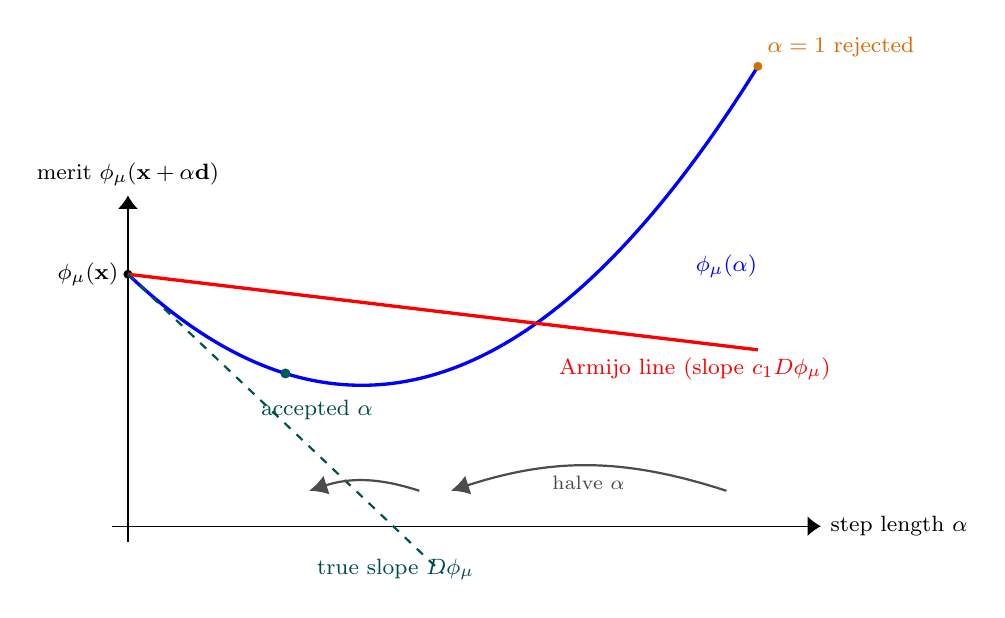
\begin{tikzpicture}[
    >={Latex[width=2.5mm]},
    every node/.style={font=\footnotesize},
    scale=1.0,
]
\draw[->] (-0.2,0) -- (8.8,0) node[right] {step length $\alpha$};
\draw[->] (0,-0.2) -- (0,4.2) node[above] {merit $\phi_\mu(\xv+\alpha\dv)$};
% the true merit along d: dips then rises (full step overshoots)
\draw[blue, very thick, smooth, samples=80, domain=0:8, variable=\x]
   plot (\x, {3.2 - 0.95*\x + 0.16*\x*\x});
\node[blue] at (7.6,3.3) {$\phi_\mu(\alpha)$};
% phi at alpha=0
\filldraw[black] (0,3.2) circle (1.4pt);
\node[left] at (0,3.2) {$\phi_\mu(\xv)$};
% Armijo line: gentle downward line
\draw[red, very thick] (0,3.2) -- (8,{3.2 - 0.12*8});
\node[red] at (7.2,2.0) {Armijo line (slope $c_1 D\phi_\mu$)};
% tangent at 0 (the actual directional derivative, steeper)
\draw[teal!65!black, thick, dashed] (0,3.2) -- (4.0,{3.2 - 0.95*4.0});
\node[teal!60!black] at (3.4,-0.55) {true slope $D\phi_\mu$};
% acceptable region: where phi(alpha) <= Armijo line.
\filldraw[orange!85!black] (8,{3.2-0.95*8+0.16*64}) circle (1.4pt)
   node[above right]{$\alpha=1$ rejected};
\filldraw[teal!70!black] (2.0,{3.2-0.95*2+0.16*4}) circle (1.6pt);
\node[teal!60!black, below=6pt] at (2.4,{3.2-0.95*2+0.16*4}) {accepted $\alpha$};
% halving arrows
\draw[->, gray!60!black, thick] (7.6,0.45) to[bend right=18]
   node[midway,below,font=\scriptsize,text=gray!55!black]{halve $\alpha$} (4.1,0.45);
\draw[->, gray!60!black, thick] (3.7,0.45) to[bend right=18] (2.3,0.45);
\end{tikzpicture}
\caption{The Armijo backtracking line search on the $\ell_1$ merit
function, the SQP's ``how far'' decision.  The QP gives a descent
direction $\dv$; we walk along it and watch the merit
$\phi_\mu(\xv+\alpha\dv)$, which trades objective against constraint
violation.  The full step $\alpha=1$ overshoots the dip and sits
\emph{above} the gentle Armijo sufficient-decrease line (red, slope
$c_1 D\phi_\mu$ with $c_1=10^{-4}$), so it is rejected; the simulator
halves $\alpha$ until a trial point falls \emph{below} that line --- a
small but genuine merit decrease, enough to guarantee progress.  If
$\alpha$ shrinks past $10^{-8}$ with no acceptance, SQP stops honestly
rather than fake convergence --- usually the finite-difference gradients
have hit their noise floor.}
\label{fig:sqp-armijo}
\end{figure}

solver stops \emph{honestly} (``line search failed --- no merit
decrease''), rather than pretend convergence --- usually a sign the
finite-difference gradients have hit their noise floor.

\paragraph{The Maratos effect and the watchdog.}
A known pathology: near the optimum the $\ell_1$ merit can reject the
\emph{full} Newton step even though it improves both objective and
feasibility --- the \emph{Maratos effect} \cite{NocedalWright} --- which
destroys the fast local rate. Choupo's v1 mitigation is deliberately
minimal: a \emph{watchdog} that forces the full $\alpha = 1$ step every
$K = 5$ iterations regardless of the merit, breaking the merit's veto. It
also \emph{reports} the symptom (full step improved feasibility yet the
merit rejected it) so the student sees the effect, not just its cure.

\subsection{Termination: the five-residual KKT certificate}

SQP stops when the KKT conditions
\eqref{eq:kkt-stat}--\eqref{eq:kkt-compl} are met within tolerance.
Choupo measures, at the current iterate with the latest QP multipliers,
five residuals:
\begin{equation}
\begin{aligned}
   r_{\mathrm{stat}}  &= \|\nabla_{\!\xv}\mathcal L\|_\infty
     && (\le 10^{-5}), &
   r_{\mathrm{feas}}^{\mathrm{eq}}  &= \max_j |h_j|
     && (\le 10^{-6}), \\
   r_{\mathrm{feas}}^{\mathrm{ineq}} &= \max_k \max(0, g_k)
     && (\le 10^{-6}), &
   r_{\mathrm{compl}} &= \max_k |\mu_k\, g_k|
     && (\le 10^{-6}), \\
   r_{\mathrm{dual}}  &= \max_k \max(0, -\mu_k)
     && (\ge 0). &&&
\end{aligned}
\end{equation}
for stationarity, equality and inequality feasibility, complementary
slackness, and dual feasibility. When the first four clear their
tolerances the solver returns \texttt{converged}, and prints all five as
a \emph{certificate} the student can verify by hand. Active box bounds
are folded in as ordinary inequality rows in the QP, so a binding bound
contributes its multiplier into $r_{\mathrm{stat}}$ --- a bound that
holds is a genuine active constraint, not a free direction.

\subsection{The inner active-set QP}\label{ch:active-set-qp}

Every SQP iteration must solve the strictly-convex QP \eqref{eq:sqp-qp}.
Choupo does this with a hand-rolled \textbf{active-set} method
(\code{solver::activeSetQP}), the classical algorithm for convex QPs
\cite[Alg.\ 16.3]{NocedalWright}. The idea: maintain a \emph{working
set} $W$ of constraints treated as equalities (all true equality rows,
plus the inequality rows currently guessed active), and at each step
solve the equality-constrained QP over $W$ exactly via its KKT linear
system
\begin{equation}
   \begin{bmatrix} \Bv & A_W^{\!\top} \\ A_W & \mathbf 0 \end{bmatrix}
   \begin{bmatrix} \mathbf p \\ \boldsymbol\lambda_W \end{bmatrix}
   =
   \begin{bmatrix} -\mathbf g_W \\ -\mathbf c_W \end{bmatrix},
   \label{eq:eqqp-kkt}
\end{equation}
solved by the same Gauss elimination with partial pivoting as the rest

\begin{figure}[ht]
\centering
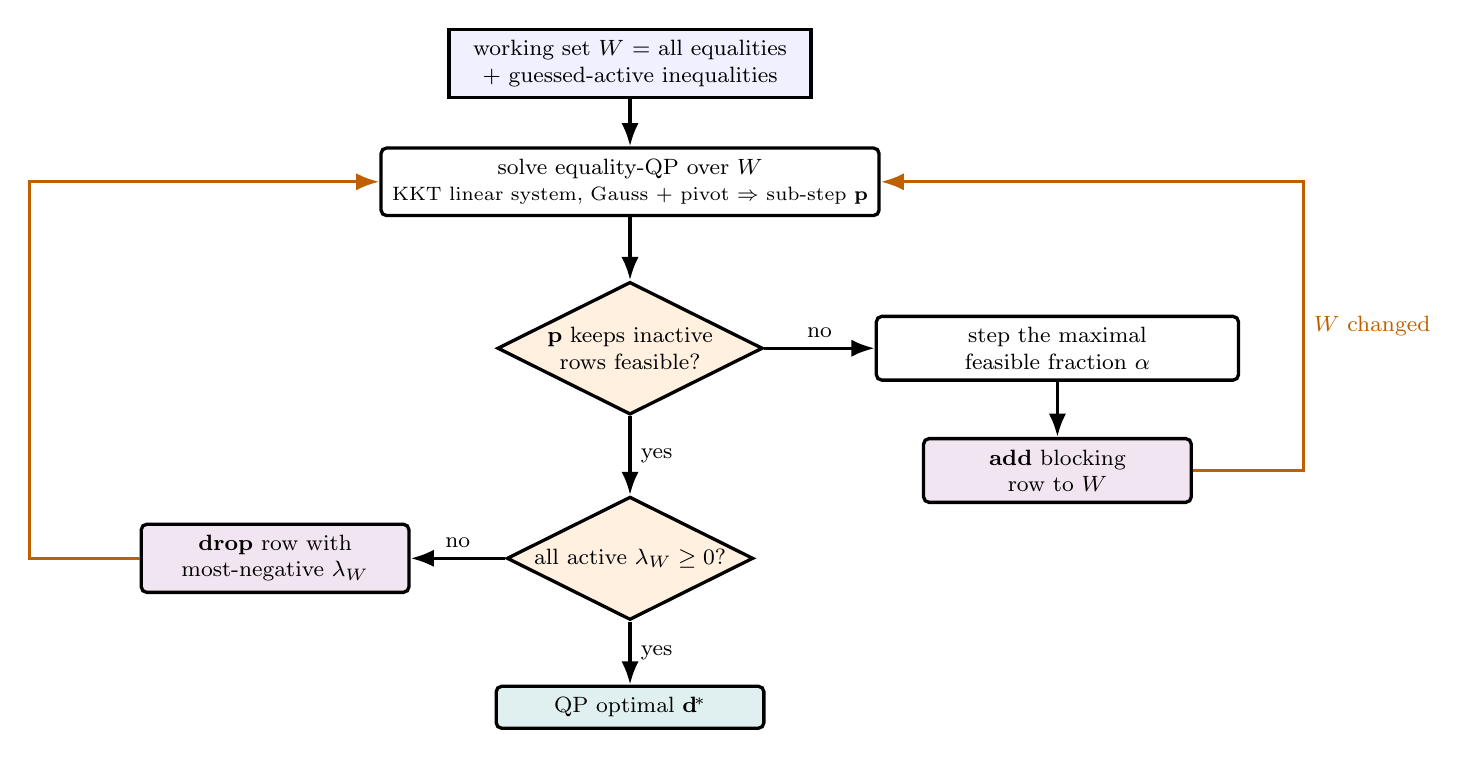
\begin{tikzpicture}[
    >={Latex[width=2.2mm]},
    every node/.style={font=\footnotesize},
    node distance = 6mm and 12mm,
    box/.style  ={draw, rounded corners=2pt, very thick, align=center,
                  inner sep=4pt, minimum width=46mm},
    io/.style   ={draw, very thick, fill=blue!6, align=center,
                  inner sep=4pt, minimum width=46mm},
    test/.style ={draw, diamond, aspect=2.0, very thick, fill=orange!12,
                  align=center, inner sep=1pt},
    add/.style  ={draw, rounded corners=2pt, very thick, fill=violet!10,
                  align=center, inner sep=4pt, minimum width=34mm},
    done/.style ={draw, rounded corners=2pt, very thick, fill=teal!12,
                  align=center, inner sep=4pt, minimum width=34mm},
    flow/.style ={->, very thick},
    loop/.style ={->, very thick, orange!75!black},
]
\node[io]  (init) {working set $W$ = all equalities\\ + guessed-active inequalities};
\node[box, below=of init] (kkt)
   {solve equality-QP over $W$\\
    {\scriptsize KKT linear system, Gauss + pivot $\Rightarrow$ sub-step $\mathbf p$}};
\node[test, below=8mm of kkt] (block)
   {$\mathbf p$ keeps inactive\\rows feasible?};
\node[box, right=14mm of block] (clip)
   {step the maximal\\ feasible fraction $\alpha$};
\node[add, below=7mm of clip] (addc) {\textbf{add} blocking\\ row to $W$};
\node[test, below=10mm of block] (mult) {all active $\lambda_W\ge 0$?};
\node[add, left=12mm of mult] (drop)
   {\textbf{drop} row with\\ most-negative $\lambda_W$};
\node[done, below=8mm of mult] (out) {QP optimal $\dv^{\!*}$};
\draw[flow] (init) -- (kkt);
\draw[flow] (kkt)  -- (block);
\draw[flow] (block) -- node[above]{no} (clip);
\draw[flow] (clip) -- (addc);
\draw[flow] (block) -- node[right]{yes} (mult);
\draw[flow] (mult) -- node[above]{no} (drop);
\draw[flow] (mult) -- node[right]{yes} (out);
% loop-backs: both add and drop re-solve with the changed W
\draw[loop] (addc.east) -- ++(1.4,0) |- node[pos=0.25,right]{$W$ changed} (kkt.east);
\draw[loop] (drop.west) -- ++(-1.4,0) |- (kkt.west);
\end{tikzpicture}
\caption{The inner active-set method that solves each SQP quadratic
program.  It maintains a \emph{working set} $W$ --- the constraints it
currently treats as equalities --- and at every pass solves the
equality-constrained QP over $W$ exactly through its KKT linear system
(the same Gauss-with-pivoting solver, Fig.~\ref{fig:lu-gauss-flow}).
Then two questions steer it: if the sub-step would cross an inactive
inequality, take the largest feasible fraction toward it and
\emph{add} that blocking row to $W$; otherwise check the active
multipliers --- if any is negative, that constraint wants to leave, so
\emph{drop} the most-negative one; if all are non-negative, the KKT
conditions hold and the QP is optimal.  Because $\Bv$ is strictly
convex, every working-set change strictly lowers the QP objective, so
the loop terminates in finitely many add/drop steps.}
\label{fig:active-set-qp}
\end{figure}

of the simulator (§\ref{ch:nrND}). Then:
\begin{itemize}
  \item If the resulting sub-step $\mathbf p$ keeps every \emph{inactive}
        inequality feasible, take it and inspect the multipliers of the
        active inequality rows. If all $\lambda_W \ge 0$ the KKT
        conditions hold over the full set --- \textbf{optimal}, return.
        Otherwise \emph{drop} the inequality with the most-negative
        multiplier from $W$ (it wants to move off its bound).
  \item If $\mathbf p$ would violate an inactive inequality, take the
        maximal feasible fraction $\alpha \in [0,1)$ toward the nearest
        \emph{blocking} constraint, stp, and \emph{add} that constraint
        to $W$.
\end{itemize}
Strict convexity of $\Bv$ guarantees a strict decrease at every
working-set change, hence \emph{finite} termination
\cite[Sec.\ 16.5]{NocedalWright}. Box bounds $\mathrm{lo} \le \dv \le
\mathrm{hi}$ are folded in as ordinary inequality rows, so one machinery
handles everything.

\paragraph{Honest failure modes.}
A singular KKT matrix \eqref{eq:eqqp-kkt} means the active constraint
gradients are linearly dependent --- a \emph{LICQ failure}. Choupo
recovers when the deficiency is among active \emph{inequalities} (drop
the most-recently-added, and forbid it from re-entering this solve,
breaking the drop/re-add cycle two nearly-parallel constraints would
form); if the deficiency is in the equality rows it is genuine and
unrecoverable, and the solver throws a clear diagnostic rather than
returning garbage. A working-set-change cap aborts loudly on suspected
cycling --- never a silent spin.

\subsection{A worked self-check: Hock--Schittkowski}

Because the SQP is finite-difference and the simulator pass is noisy,
Choupo \emph{re-proves the algorithm} before every constrained run, on
three analytic problems from the Hock--Schittkowski test set
\cite{HockSchittkowski} (\code{verifySQP}, a merge-blocking gate). Take
\textbf{HS35} (Beale):
\begin{equation}
\begin{aligned}
   \min_{\xv \ge 0} \; & 9 - 8x_1 - 6x_2 - 4x_3
     + 2x_1^2 + 2x_2^2 + x_3^2 + 2x_1x_2 + 2x_1x_3 \\
   \text{s.t.}\;\; & x_1 + x_2 + 2x_3 \le 3,
\end{aligned}
\end{equation}
whose published optimum is $f^\star = \tfrac19 = 0.1111\ldots$ at
$\xv^\star = (\tfrac43, \tfrac79, \tfrac49)$. From $\xv_0 =
(\tfrac12,\tfrac12,\tfrac12)$ Choupo's SQP linearises (one constraint
row plus three lower-bound rows), solves the convex QP, damped-BFGS
updates $\Bv$, and converges to $|f - f^\star| < 10^{-4}$. The companion
\code{verifyActiveSetQP} solves a hand-worked three-inequality QP whose
active set $\{d_1 + d_2 \le 1\}$, primal solution $\dv^\star = (0,1)$ and
multipliers $\boldsymbol\mu = (1, 0, 0)$ are known by hand, and asserts
the inner solver reproduces them to $10^{-9}$. If either self-check
fails the run aborts --- the tolerance is never loosened to mask a bug.

\paragraph{Power and limit.} \textbf{Power:} SQP is the method of choice
for smooth, equality- and inequality-constrained NLPs --- it honours
hard constraints exactly at the solution, returns shadow-price
multipliers for free, and converges superlinearly near the optimum
because $\Bv$ approximates the Lagrangian curvature. A flowsheet
DesignSpec, a purity floor, or a duty-equals-target all map directly
onto \eqref{eq:sqp-nlp}. \textbf{Limit:} it is a \emph{local} method
(converges to the nearest KKT point --- multi-start for global search),
the gradients are finite-difference so it inherits the simulator's noise
floor (a noisy pass poisons $\Bv$ and the merit), and it assumes the
responses are smooth in $\xv$ --- a discrete decision or a
phase-appearance discontinuity breaks the linearisation. For a black-box
\emph{unconstrained} objective with no derivatives, reach back for
Nelder-Mead (§\ref{ch:nelder-mead}); SQP earns its keep precisely when
the constraints are real.

\subsection*{What you see in Choupo}

Selecting \code{method sqp;} in an \code{outerDict} optimisation block
makes \code{OptimizationDriver} print, per iteration, the damped-BFGS
$\theta$, the merit penalty $\mu$, the active set, the Lagrange
multipliers (shadow prices), the Armijo step $\alpha$, and the four KKT
residuals --- the whole inner workings, not just a final answer. The
self-checks \code{verifySQP} / \code{verifyActiveSetQP} run first and
their pass is announced. On convergence the five-line KKT certificate is
printed and the simulator is replayed once at the optimum with full
verbosity, exactly as the Nelder-Mead path does.

% ---------------------------------------------------------------------
\section{Runge-Kutta 4 for the PFR}\label{ch:rk4}

\begin{whatyoulllearn}
The PFR model integrates concentrations along the reactor volume by
the canonical fourth-order Runge-Kutta scheme. The independent
variable is $V$, not $t$ --- a small but important reinterpretation.
\end{whatyoulllearn}

\subsection{The reactor as an ODE}

In a steady-state PFR with molar flow rate $F$ and reaction extent per
unit volume $\dot r$:
\begin{equation}
   \frac{d \xv}{d V} \;=\; \frac{\boldsymbol\nu \cdot r(\xv, T)}{F},
\end{equation}
with $\boldsymbol\nu$ the stoichiometric vector and $\xv$ the mole-fraction
vector along the reactor. The state $\xv$ at $V = V_R$ is the outlet.

\subsection{RK4 step}

For a step of size $h = V_R / N$:
\begin{align}
   \mathbf{k}_1 &= f(\xv_n) \\
   \mathbf{k}_2 &= f(\xv_n + \tfrac{h}{2}\,\mathbf{k}_1) \\
   \mathbf{k}_3 &= f(\xv_n + \tfrac{h}{2}\,\mathbf{k}_2) \\
   \mathbf{k}_4 &= f(\xv_n + h\,\mathbf{k}_3) \\
   \xv_{n+1}    &= \xv_n + \tfrac{h}{6}\,(\mathbf{k}_1 + 2\mathbf{k}_2 + 2\mathbf{k}_3 + \mathbf{k}_4)
\end{align}
Local truncation error is $O(h^5)$ per step; global error is $O(h^4)$.
At $N = 100$ (the simulator's default) this is well below the
significance of any kinetics one can realistically know.

% --- Figure: RK4 stage structure -------------------------------------
\begin{figure}[h]
\centering
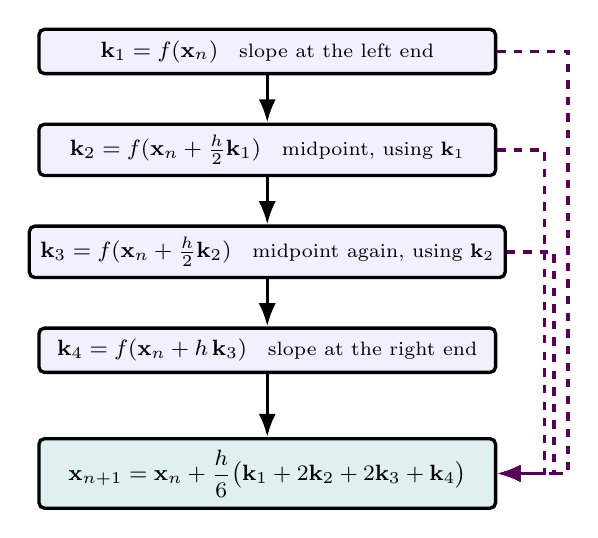
\begin{tikzpicture}[
    >={Latex[width=2.2mm]},
    every node/.style={font=\footnotesize},
    stage/.style={draw, rounded corners=2pt, very thick, align=center,
                  inner sep=4pt, minimum width=58mm, fill=blue!6},
    comb/.style ={draw, rounded corners=2pt, very thick, align=center,
                  inner sep=4pt, minimum width=58mm, fill=teal!12},
    flow/.style ={->, very thick},
    use/.style  ={->, very thick, violet!70!black, dashed},
]
\node[stage] (k1) {$\mathbf k_1=f(\xv_n)$ \;\;\scriptsize slope at the left end};
\node[stage, below=6mm of k1] (k2)
     {$\mathbf k_2=f(\xv_n+\tfrac h2\mathbf k_1)$ \;\;\scriptsize midpoint, using $\mathbf k_1$};
\node[stage, below=6mm of k2] (k3)
     {$\mathbf k_3=f(\xv_n+\tfrac h2\mathbf k_2)$ \;\;\scriptsize midpoint again, using $\mathbf k_2$};
\node[stage, below=6mm of k3] (k4)
     {$\mathbf k_4=f(\xv_n+h\,\mathbf k_3)$ \;\;\scriptsize slope at the right end};
\node[comb,  below=8mm of k4] (cmb)
     {$\xv_{n+1}=\xv_n+\dfrac h6\bigl(\mathbf k_1+2\mathbf k_2+2\mathbf k_3+\mathbf k_4\bigr)$};
\draw[flow] (k1) -- (k2);
\draw[flow] (k2) -- (k3);
\draw[flow] (k3) -- (k4);
\draw[flow] (k4) -- (cmb);
% the four slopes all feed the weighted combination
\draw[use] (k1.east) -- ++(0.9,0) |- (cmb.east);
\draw[use] (k2.east) -- ++(0.6,0) |- (cmb.east);
\draw[use] (k3.east) -- ++(0.6,0) |- (cmb.east);
\end{tikzpicture}
\caption{The four-stage structure of classical RK4 for one step
$\xv_n\to\xv_{n+1}$ of size $h$ (here $h=V_R/N$ marching down the PFR).
Each stage is one evaluation of the right-hand side $f$: a slope at the
left end ($\mathbf k_1$), two probes of the midpoint slope that reuse
the previous stage ($\mathbf k_2,\mathbf k_3$), and a slope at the right
end ($\mathbf k_4$).  The solid arrows are the data dependency --- each
$\mathbf k$ feeds the next --- and the dashed violet arrows show all
four slopes returning to be combined with Simpson-like weights
$1{:}2{:}2{:}1$.  That weighting is exactly what buys the $O(h^5)$
local accuracy from only four function calls.  The same packed-state
machinery drives the batch integrators of
Chapter~\ref{ch:rk4-packed}.}
\label{fig:rk4-stages}
\end{figure}

% =====================================================================
% PART IV --- TRANSPORT PROPERTIES AND MIXING RULES
% =====================================================================
\clearpage
\section*{Part V --- Transport properties and mixing rules}
\phantomsection
\addcontentsline{toc}{section}{Part V --- Transport properties and mixing rules}

\stepcounter{thpart}
\setcounter{section}{0}

% ---------------------------------------------------------------------
\section{Why transport: where pressure drop, heat transfer, and HETP come from}\label{ch:why-transport}

\begin{whatyoulllearn}
A flash needs no transport coefficients --- the answer depends only
on phase equilibrium.  A packed column, a tube-side heat exchanger
or a fixed-bed reactor lives or dies on viscosity, thermal
conductivity and diffusivity.  This Part introduces those three
property families in the Reid-Prausnitz-Poling tradition (classic,
non-cubic models, two or three parameters per pure component, plus a
mixture rule per property), documents the planned extension of the
\file{*.dat} schema, and points forward to the unit-operation
correlations they feed.
\end{whatyoulllearn}

\subsection{Three coefficients, three modes of irreversibility}

Thermodynamics tells you where a system wants to go.  Transport tells
you how fast it gets there and what it costs.  Three Newtonian
constitutive laws --- one per mode of irreversibility --- show up in
every unit operation that involves flow, heat or mass transfer:

\begin{center}\small
\begin{tabular}{@{}llll@{}}
\toprule
mode      & flux            & gradient driver       & coefficient \\
\midrule
momentum  & $\tau$ (Pa)     & $\partial u / \partial y$ & viscosity $\mu$ \\
heat      & $q$ (W/m²)      & $\partial T / \partial y$ & thermal conductivity $\kappa$ \\
mass (i)  & $J_i$ (mol/m²s) & $\partial c_i / \partial y$ & diffusivity $D_i$ \\
\bottomrule
\end{tabular}
\end{center}

Newton's law of viscosity ($\tau = -\mu\,\mathrm{d}u/\mathrm{d}y$),
Fourier's law of heat conduction ($q = -\kappa\,\mathrm{d}T/\mathrm{d}y$)
and Fick's first law of diffusion ($J_i = -D_i\,\mathrm{d}c_i/\mathrm{d}y$)
share the same linear-response form.  Each transport coefficient is
a \emph{thermophysical} property of the fluid: it depends on $T$,
mildly on $P$ (strongly for gases above $\sim$10~bar), and on
composition.  Unlike thermodynamic properties they describe
irreversible processes; they do not derive from an energy.

\begin{intuition}
A common student trap is to expect that, just like enthalpy follows
from $c_p$, viscosity should follow from something equally
fundamental.  It does not.  Transport coefficients ultimately come
from the underlying kinetic theory --- collision integrals for
gases, free-volume theory for liquids --- but for engineering work
we use \emph{correlations}: 2-3-parameter fits to empirical data,
identical in spirit to Antoine for vapour pressure.
\end{intuition}

\subsection{Where each property is consumed}

\begin{figure}[ht]
\centering
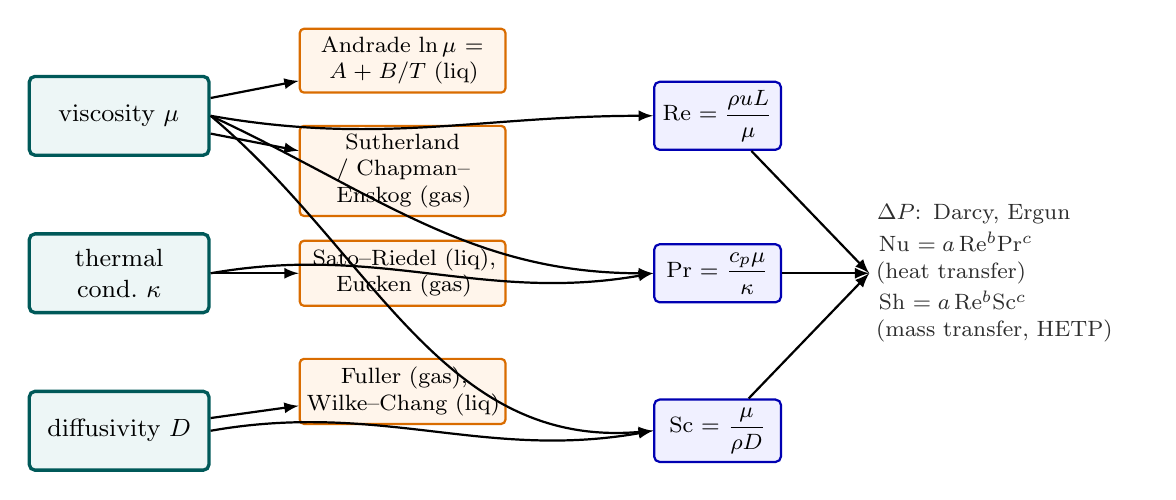
\begin{tikzpicture}[
    prop/.style={draw, very thick, rounded corners=2pt, align=center,
                 font=\small, inner sep=4pt, minimum height=10mm,
                 fill=teal!7, draw=teal!70!black, text width=20mm},
    corr/.style={draw, thick, rounded corners=1.5pt, align=center,
                 font=\footnotesize, inner sep=3pt, minimum height=7mm,
                 fill=orange!8, draw=orange!85!black, text width=24mm},
    grp/.style={draw, thick, rounded corners=2pt, align=center,
                font=\footnotesize, fill=blue!6, draw=blue!70!black,
                inner sep=3pt, text width=14mm},
    use/.style={font=\footnotesize, align=left, text=gray!35!black,
                text width=33mm},
    flow/.style={->, >=latex, thick},
]
\node[prop] (mu)  at (0,4.0) {viscosity $\mu$};
\node[prop] (k)   at (0,2.0) {thermal cond.\ $\kappa$};
\node[prop] (d)   at (0,0.0) {diffusivity $D$};
\node[corr] (andr) at (3.6,4.7) {Andrade $\ln\mu=A+B/T$ (liq)};
\node[corr] (suth) at (3.6,3.3) {Sutherland / Chapman--Enskog (gas)};
\node[corr] (sato) at (3.6,2.0) {Sato--Riedel (liq), Eucken (gas)};
\node[corr] (fwc)  at (3.6,0.5) {Fuller (gas), Wilke--Chang (liq)};
\node[grp] (re) at (7.6,4.0) {Re $=\dfrac{\rho uL}{\mu}$};
\node[grp] (pr) at (7.6,2.0) {Pr $=\dfrac{c_p\mu}{\kappa}$};
\node[grp] (sc) at (7.6,0.0) {Sc $=\dfrac{\mu}{\rho D}$};
\node[use] (cons) at (11.3,2.0)
   {$\Delta P$: Darcy, Ergun\\[2pt] Nu $=a\,$Re$^b$Pr$^c$\\ (heat transfer)\\[2pt] Sh $=a\,$Re$^b$Sc$^c$\\ (mass transfer, HETP)};
\draw[flow] (mu) -- (andr);
\draw[flow] (mu) -- (suth);
\draw[flow] (k)  -- (sato);
\draw[flow] (d)  -- (fwc);
\draw[flow] (mu.east) to[out=-10,in=180] (re.west);
\draw[flow] (mu.east) to[out=-25,in=180] (pr.west);
\draw[flow] (k.east)  to[out=10,in=190] (pr.west);
\draw[flow] (mu.east) to[out=-40,in=185] (sc.west);
\draw[flow] (d.east)  to[out=10,in=190] (sc.west);
\draw[flow] (re) -- (cons.west);
\draw[flow] (pr) -- (cons.west);
\draw[flow] (sc) -- (cons.west);
\end{tikzpicture}
\caption{The transport map: three coefficients, their correlations, and
where they are consumed.  Each Newtonian coefficient (teal) is supplied by
a two- or three-parameter correlation (orange)---Andrade or
Sutherland/Chapman--Enskog for viscosity, Sato--Riedel/Eucken for
conductivity, Fuller and Wilke--Chang for diffusivity.  The coefficients
then assemble into the three dimensionless groups Re, Pr, Sc (blue), and
nearly every downstream design equation is a power law in them
($\mathrm{Nu}=a\,\mathrm{Re}^b\mathrm{Pr}^c$,
$\mathrm{Sh}=a\,\mathrm{Re}^b\mathrm{Sc}^c$).  Note that viscosity feeds
all three groups---one good $\mu$ correlation unlocks pressure drop, heat
\emph{and} mass transfer.}
\label{fig:transport-map}
\end{figure}


\begin{center}\small
\begin{tabular}{@{}lll@{}}
\toprule
property & feeds & through correlation\\
\midrule
viscosity $\mu$       & pressure drop in tubes, packings    & Darcy-Weisbach, Ergun \\
                      & shear-controlled mixing             & power number correlations \\
                      & convective heat transfer            & Dittus-Boelter (turbulent), Sieder-Tate \\
                      & column flooding limits              & Souders-Brown coefficient \\[2pt]
thermal cond.\ $\kappa$ & conductive heat transfer          & Fourier across pipe walls / fins \\
                      & convective heat transfer            & via Nusselt = $f$(Re, Pr) \\[2pt]
diffusivity $D$       & mass-transfer coefficient          & Sherwood = $f$(Re, Sc) \\
                      & HETP / NTU in absorption, dist.\ & Onda, Eduljee \\
                      & gas-side concentration polarisation & Sherwood again \\
\bottomrule
\end{tabular}
\end{center}

\begin{intuition}
The three dimensionless groups Re ($= \rho u L / \mu$), Pr ($= c_p
\mu / \kappa$) and Sc ($= \mu / (\rho D)$) capture each property's
role in a heat- or mass-transfer correlation, normalised against the
flow.  Most empirical Nusselt or Sherwood relations are functions of
the form Nu $= a$ Re$^b$ Pr$^c$ or Sh $= a$ Re$^b$ Sc$^c$, so
\emph{one good correlation per coefficient} unlocks the entire family
of design equations downstream.
\end{intuition}

\subsection{Status note}

None of this is implemented yet.  Pressure drops in the simulator are
zero; heat-exchanger duties bypass the $U A$ product (a Tout or $Q$
is given, not derived from area); column efficiency is taken as 100\%
per stage.  Part IV documents the theory and the planned data-file
extension; the C++ wiring is on the v1.x roadmap.  Every chapter that
follows closes with a candid status note.

% ---------------------------------------------------------------------
\section{Viscosity}\label{ch:viscosity}

\begin{whatyoulllearn}
The viscosity of a pure liquid follows the Andrade equation $\ln \mu
= A + B/T$ --- a two-parameter fit that captures the strong
Arrhenius-like decay of liquid viscosity with temperature.  Gases
take the opposite trend ($\mu$ grows with $T$); the classical model
is Sutherland.  The corresponding-states alternative for either
phase is the Chapman-Enskog formula in terms of Lennard-Jones $\sigma$
and $\epsilon/k$.  Reid-Prausnitz-Poling Chapter~9.
\end{whatyoulllearn}

\subsection{Pure liquid: Andrade}

\begin{figure}[ht]
\centering
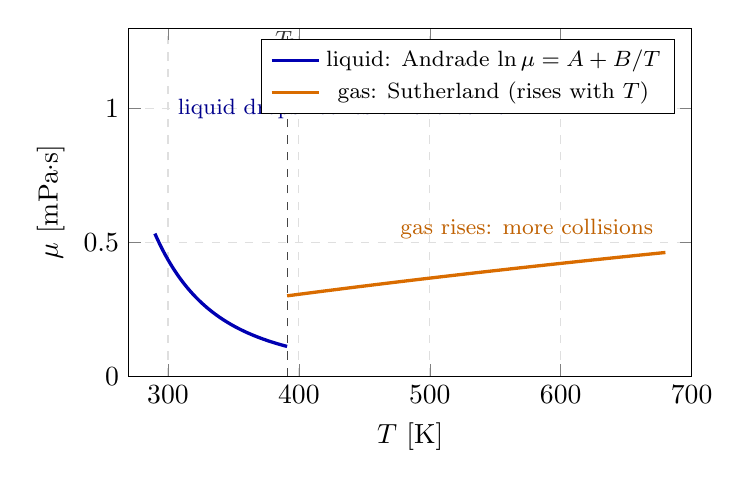
\begin{tikzpicture}
\begin{axis}[
    width=0.72\linewidth, height=6cm,
    xlabel={$T$ [K]},
    ylabel={$\mu$ [mPa$\cdot$s]},
    xmin=270, xmax=700,
    ymin=0, ymax=1.3,
    grid=major,
    grid style={gray!25, dashed},
    legend pos=north east,
    legend style={font=\footnotesize},
]
\addplot[domain=290:391, samples=60, blue!70!black, very thick]
   ({x},{1000*exp(-13.61 + 1761/x)});
\addlegendentry{liquid: Andrade $\ln\mu=A+B/T$}
\addplot[domain=391:680, samples=60, orange!85!black, very thick]
   ({x},{0.30*(x/391)^1.5*(391+200)/(x+200)});
\addlegendentry{gas: Sutherland (rises with $T$)}
\node[font=\footnotesize, text=blue!55!black, anchor=west] at (axis cs:300,1.0)
   {liquid drops: cohesion overcome};
\node[font=\footnotesize, text=orange!75!black, anchor=west] at (axis cs:470,0.55)
   {gas rises: more collisions};
\draw[dashed, gray!55!black] (axis cs:391,0) -- (axis cs:391,1.3);
\node[font=\footnotesize, text=gray!45!black, anchor=south] at (axis cs:391,1.18) {$T_b$};
\end{axis}
\end{tikzpicture}
\caption{Liquid and gas viscosity move in \emph{opposite} directions with
temperature---the most counter-intuitive fact in transport.  Below
the boiling point the liquid follows Andrade
($\ln\mu=A+B/T$, blue): viscosity falls steeply as thermal energy lets
molecules slip past one another.  Above it the gas follows Sutherland
(orange): viscosity \emph{rises} because hotter molecules carry more
momentum across the shear gradient.  Curves are illustrative (acetic-acid
liquid constants $A=-13.61$, $B=1761$~K; the gas branch is a
representative Sutherland shape, not to the same vertical scale).}
\label{fig:viscosity-trends}
\end{figure}


Liquid viscosity drops sharply with temperature because molecules
move past each other more easily once thermal energy starts to
overcome the cohesive potential.  The empirical fit is
\begin{equation}
   \boxed{\;
   \ln \mu^{\mathrm{liq}}(T) \;=\; A \;+\; \frac{B}{T},
   \;}\qquad \mu \text{ in Pa$\cdot$s, } T \text{ in K.}
   \label{eq:andrade}
\end{equation}
Two parameters, fitted to two or more $(\mu, T)$ data points.  For
the practically interesting range $0.4\,T_c < T < 0.95\,T_c$ this
two-parameter form is within $\sim$5\% of experimental viscosity.
For wider ranges (cryogenic to near-critical) Reid recommends the
extended four-parameter Andrade
\begin{equation}
   \ln \mu^{\mathrm{liq}}(T) \;=\;
     A \;+\; \frac{B}{T} \;+\; C\,\ln T \;+\; D\,T^E,
\end{equation}
but the two-parameter form is what we ship.

\begin{example}[Acetic acid at 300 K and 380 K]
Fitting Andrade to two literature data points ($\mu(300) = 1.07$ mPa·s,
$\mu(380) = 0.38$ mPa·s) gives $A = -13.61$, $B = 1761$~K.  At an
intermediate $T = 340$~K, Eq.~\eqref{eq:andrade} predicts $\mu(340)
\approx 0.63$ mPa·s, against a measured $\approx 0.60$ mPa·s --- a
5\% prediction without any 340~K measurement.
\end{example}

\subsection{Pure gas: Sutherland}

Gas viscosity \emph{increases} with temperature: more thermal energy
means more momentum-carrying collisions across a flow gradient.  The
classical fit is Sutherland (originally derived from a square-well
potential),
\begin{equation}
   \boxed{\;
   \mu^{\mathrm{gas}}(T) \;=\; \mu_0\,
     \left(\frac{T}{T_0}\right)^{3/2}\,
     \frac{T_0 + S}{T + S},
   \;}
   \label{eq:sutherland}
\end{equation}
where $\mu_0$ is the viscosity at the reference temperature $T_0$
(commonly 273.15~K) and $S$ is the Sutherland constant (a positive
material parameter that controls the deviation from $T^{1/2}$
behaviour of hard-sphere theory).  Three parameters per component.
Air: $\mu_0 = 1.716 \times 10^{-5}$~Pa·s, $T_0 = 273.15$~K,
$S = 110.4$~K.

\subsection{Either phase: Chapman-Enskog with Lennard-Jones}

A corresponding-states alternative falls out of kinetic theory.  For
a dilute gas of molecules interacting through a Lennard-Jones (12--6)
pair potential characterised by $\sigma$ (collision diameter, in
ångström) and $\epsilon / k$ (well depth normalised to Boltzmann's
constant, in K),
\begin{equation}
   \mu^{\mathrm{gas}}(T) \;=\;
     2.6693 \times 10^{-6}\,
     \frac{\sqrt{M\,T}}{\sigma^{2}\,\Omega_{\!\mu}(T^*)}
     \qquad \text{[Pa$\cdot$s; $M$ in kg/kmol; $T$ in K; $\sigma$ in Å]},
   \label{eq:chapman-enskog}
\end{equation}
where $T^* = kT / \epsilon$ and the dimensionless collision integral
$\Omega_{\!\mu}$ is tabulated (Reid Table 9-2) or approximated by the
Neufeld correlation
\begin{equation}
   \Omega_{\!\mu}(T^*) \;\approx\; \frac{1.16145}{(T^*)^{0.14874}}
     \;+\; \frac{0.52487}{e^{0.7732\,T^*}}
     \;+\; \frac{2.16178}{e^{2.43787\,T^*}}.
\end{equation}
The appeal of the LJ approach is that \emph{two} parameters
($\sigma$, $\epsilon/k$) determine viscosity, thermal conductivity
and diffusivity --- not separately fitted per property.  Tabulations
exist for most common species.

\subsection{The Chung correlation --- what Choupo actually uses}
The Lennard-Jones form needs $\sigma$ and $\epsilon/k$, which are tabulated
for only some species.  Choupo instead ships the \textbf{Chung et al.\ (1988)}
corresponding-states realisation of the SAME kinetic theory, which ESTIMATES
the collision parameters from the critical properties every component already
carries --- so a gas viscosity follows from $T_c, P_c, \omega, M$ alone, with
no separate viscosity datum:
\begin{equation}
  \mu^{\mathrm{gas}}(T) \;=\; 40.785 \times 10^{-7}\;
     \frac{F_c\,\sqrt{M\,T}}{V_c^{2/3}\,\Omega_{\!\mu}(T^*)}
     \qquad\text{[Pa$\cdot$s; $M$ in kg/kmol; $V_c$ in cm$^3$/mol]},
  \label{eq:chung-viscosity}
\end{equation}
with the critical volume from the acentric-corrected compressibility
$V_c = Z_c R T_c / P_c$, $Z_c = 0.2918 - 0.0928\,\omega$; the reduced
temperature $T^* = 1.2593\,T/T_c$ feeding the SAME Neufeld collision integral
$\Omega_{\!\mu}$; and the polarity factor $F_c = 1 - 0.2756\,\omega$ (non-polar
here --- the factor does not capture strong dipoles, so Chung degrades for
polar species).  For a simple non-polar gas the accuracy is excellent: at
298~K it returns $\mu_{\mathrm{N_2}} = 1.78\times10^{-5}$~Pa$\cdot$s, within
$\sim$0.3\% of the measured value.  The model is DECLARED
(\code{transport \{ model Chung; \}} in the thermoPackage) and the engine
REFUSES to guess a viscosity without it --- no silent default.  (Water and
steam take the higher-accuracy IAPWS transport formulation instead.)

\subsection{Data-file extension (optional per-component override)}

The Chung/Sutherland corresponding-states route above needs no per-component
viscosity datum.  A component MAY still carry an explicit measured correlation
to OVERRIDE the estimate where higher accuracy is warranted:
\begin{lstlisting}
viscosityLiq
{
    model         Andrade;
    coefficients  (A B);             // ln mu_Pa.s = A + B/T
    Trange        (270 390);
}

viscosityGas
{
    model         Sutherland;
    coefficients  (mu0 T0 S);        // [Pa.s], [K], [K]
    Trange        (200 700);
}

lennardJones
{
    sigma         3.617;             // angstrom
    epsOverK      97.0;              // K
}
\end{lstlisting}

\begin{tutoriallink}
\textbf{Status note.}  No viscosity model is wired into any unit
op.  When this lands (v1.x), the call site will be
\code{ProcessStream::viscosity(T, x)} consumed by
\code{HeatExchanger}, \code{PFR} (for the Reynolds number), and
\code{DistillationColumn} (for flooding checks).
\end{tutoriallink}

% ---------------------------------------------------------------------
\section{Thermal conductivity}\label{ch:thermal-cond}

\begin{whatyoulllearn}
Liquid thermal conductivity is well represented by the Sato-Riedel
correlation --- a corresponding-states formula that needs only $M$,
$T_c$ and $T_b$ (data the simulator already has).  Gas conductivity
follows from the viscosity through Eucken's relation
$\kappa = (\mu / M)(c_p + 5R/4)$ or the modified Eucken with a
correction for polyatomics.  Reid Chapter~10.
\end{whatyoulllearn}

\subsection{Pure liquid: Sato-Riedel}

\begin{equation}
   \boxed{\;
   \kappa^{\mathrm{liq}}(T) \;=\;
     \frac{1.11}{\sqrt{M}}\,
     \frac{3 + 20\,(1 - T_r)^{2/3}}{3 + 20\,(1 - T_{br})^{2/3}}
     \qquad [\text{W/(m$\cdot$K)}],
   \;}
   \label{eq:sato-riedel}
\end{equation}
where $T_r = T / T_c$, $T_{br} = T_b / T_c$ and $M$ is in g/mol
(equivalently kg/kmol).  The formula contains zero fitted constants
per component --- it is pure corresponding states, calibrated once
across the Reid-Prausnitz-Poling reference set.  Accuracy:
$\sim$8\% on average across non-polar liquids, $\sim$15\% for polar
ones (water is an outlier and gets its own tabulation).

\begin{example}[Acetic acid at 350 K]
With $M = 60.052$, $T_c = 591.95$, $T_b = 391.05$:  $T_r = 0.591$,
$T_{br} = 0.661$.  Eq.~\eqref{eq:sato-riedel} gives
$\kappa \approx 0.162$ W/(m·K) against a literature value of
$\sim$0.158 W/(m·K).
\end{example}

\subsection{Pure gas: modified Eucken}

Eucken combined heat conduction and viscosity through the kinetic
energy budget of a colliding-molecule model:
\begin{equation}
   \boxed{\;
   \kappa^{\mathrm{gas}}(T) \;=\;
     \frac{\mu(T)}{M}\,\bigl[\,c_p(T) + \tfrac{5}{4}R\,\bigr]
     \qquad [\text{W/(m$\cdot$K)}].
   \;}
   \label{eq:eucken}
\end{equation}
The factor $\tfrac{5}{4}R$ corrects an Euler-type derivation that
otherwise overpredicts $\kappa$ for monatomics.  Polyatomic
molecules carry extra internal degrees of freedom; the
\emph{modified Eucken} replaces the kernel with $(c_p + 1.32 R)$ or
similar.  Either way, gas thermal conductivity is a derived quantity
in this scheme --- no new fitted parameter beyond those already in
$\mu$ and $c_p$.

\subsection{Data-file extension (v1.x)}

Sato-Riedel needs no coefficients; modified Eucken needs none either
once $\mu$ and $c_p$ are in place.  The data file just declares
which model to use:
\begin{lstlisting}
thermalConductivityLiq  { model SatoRiedel; }
thermalConductivityGas  { model modifiedEucken; }
\end{lstlisting}

\begin{tutoriallink}
\textbf{Status note.}  $\kappa$ is not consumed by any unit
op.  When the cubic EOS work brings real-gas heat exchangers
(v1.x), the call site will be \code{ProcessStream::kappa(T, x)}.
\end{tutoriallink}

% ---------------------------------------------------------------------
\section{Diffusivity}\label{ch:diffusivity}

\begin{whatyoulllearn}
Diffusivity is fundamentally a \emph{pair} property: it describes
the motion of species $i$ relative to species $j$, and an isolated
component cannot carry a single number.  For binary diffusion in
gases the workhorse is Fuller-Schettler-Giddings; for binary
diffusion in dilute liquids it is Wilke-Chang.  Multicomponent
extensions (Vignes, Maxwell-Stefan) build on the binary values.
Reid Chapters~11--12.
\end{whatyoulllearn}

\subsection{Gas binary: Fuller-Schettler-Giddings}

\begin{equation}
   \boxed{\;
   D_{AB}(T, P) \;=\;
     \frac{1.013 \times 10^{-7}\,T^{1.75}\,[(M_A + M_B)/(M_A M_B)]^{1/2}}
          {P\,\bigl[(\Sigma v)_A^{1/3} + (\Sigma v)_B^{1/3}\bigr]^2}
     \qquad [\text{m²/s; $T$ in K, $P$ in bar, $M$ in g/mol}].
   \;}
   \label{eq:fuller}
\end{equation}
The $(\Sigma v)_i$ are \emph{atomic diffusion volumes}: a small
table of element-additive contributions (C: 16.5, H: 1.98, O: 5.48,
N: 5.69; complete tables in Reid 11-1).  No experimental binary
diffusivity is needed --- the prediction is geometric, from atomic
group contributions only.  Accuracy: $\sim$10\% for gases at
$\sim$1~bar; degrades sharply above 10 bar where high-pressure
corrections become necessary.

\subsection{Liquid binary, dilute: Wilke-Chang}

\begin{equation}
   \boxed{\;
   D_{AB}^{\infty} \;=\;
     7.4 \times 10^{-12}\,
     \frac{(\phi_B\,M_B)^{1/2}\,T}{\mu_B\,V_A^{0.6}}
     \qquad [\text{m²/s; $T$ in K, $M$ in g/mol, $\mu_B$ in Pa·s, $V_A$ in cm³/mol}],
   \;}
   \label{eq:wilke-chang}
\end{equation}
where $V_A$ is the molar volume of solute $A$ at its boiling point
(LeBas group-contribution table, or just $V^{\mathrm{liq}}_A$ from
the data file as a first approximation) and $\phi_B$ is the
association factor of solvent $B$ (water: 2.6; methanol: 1.9;
ethanol: 1.5; benzene/other unassociated: 1.0).  The result is the
\emph{infinite-dilution} diffusivity --- valid as $x_A \to 0$.

\begin{intuition}
Liquid diffusivities are six to seven orders of magnitude lower
than gas diffusivities at 1~bar ($\sim 10^{-9}$ vs $\sim 10^{-5}$
m²/s).  This single fact is why almost every mass-transfer-limited
unit op is dominated by the liquid film resistance.
\end{intuition}

\subsection{Composition dependence: Vignes}

Wilke-Chang gives only the limiting values $D_{AB}^{\infty}$ (solute
$A$ in solvent $B$) and $D_{BA}^{\infty}$ (the reverse).  Across the
full composition range Vignes interpolates logarithmically:
\begin{equation}
   D_{AB}(x_A) \;=\; \bigl(D_{AB}^{\infty}\bigr)^{1 - x_A}\,
                     \bigl(D_{BA}^{\infty}\bigr)^{x_A}.
   \label{eq:vignes}
\end{equation}
For multicomponent systems the Maxwell-Stefan framework promotes
each binary $D_{ij}$ to a matrix that combines them rigorously.
Reid Chapter~12 treats this in depth; we will not need it before
v1.x of the simulator.

\subsection{Data-file extension (v1.x)}

Single-component files carry no diffusivity entries (diffusion is a
pair property).  Binary pairs get their own files alongside
\file{constant/binaryPairs/}:
\begin{lstlisting}
data/standards/diffusionVolumes/ethanol.dat  // for Fuller
{ sumV  50.36; }                              // atomic-volume sum

data/standards/associationFactors/water.dat   // for Wilke-Chang
{ phi   2.6; }
\end{lstlisting}

\begin{tutoriallink}
\textbf{Status note.}  Diffusivity is unused.  When mass-transfer
correlations land (post-v1, for the membrane/NF chapter that
motivates the project) the call site will be
\code{ProcessStream::Dij(T, P, x, i, j)}.
\end{tutoriallink}

% ---------------------------------------------------------------------
\section{Mixture rules}\label{ch:mixture-rules}

\begin{whatyoulllearn}
Pure-component transport properties are useless on their own ---
every real stream is a mixture.  Reid-Prausnitz-Poling Chapter~9
recommends Wilke's rule for gas viscosity, a log-mole-fraction
average for liquid viscosity, a mass-fraction average for liquid
thermal conductivity, and the Vignes interpolation for binary
diffusivity.  Each rule has a domain of validity and a
ten-line implementation.
\end{whatyoulllearn}

\subsection{Gas viscosity: Wilke}

\begin{equation}
   \mu^{\mathrm{gas}}_{\mathrm{mix}} \;=\;
     \sum_i \frac{y_i\,\mu_i}{\sum_j y_j\,\phi_{ij}},
   \qquad
   \phi_{ij} \;=\;
     \frac{\bigl[1 + (\mu_i/\mu_j)^{1/2}(M_j/M_i)^{1/4}\bigr]^2}
          {\bigl[8(1 + M_i/M_j)\bigr]^{1/2}}.
   \label{eq:wilke-rule}
\end{equation}
The $\phi_{ij}$ are dimensionless interaction terms.  Reid reports
$\sim$2\% accuracy for binary gas mixtures across the full
composition range, with the rule reducing exactly to $\mu_i$ in the
pure-component limit by construction.

\subsection{Liquid viscosity: log-mole-fraction average}

\begin{equation}
   \ln \mu^{\mathrm{liq}}_{\mathrm{mix}} \;=\;
     \sum_i x_i\,\ln \mu_i.
   \label{eq:liq-visc-mix}
\end{equation}
The motivation is empirical (Arrhenius rule for ideal liquid
mixtures) but the form is well behaved: it is exact when the mixing
is athermal and the simplest non-trivial answer otherwise.  For
strongly hydrogen-bonded mixtures the Grunberg-Nissan correction
adds a binary interaction term $\sum_i \sum_j x_i x_j G_{ij}$ but
we will not need it.

\subsection{Liquid thermal conductivity: mass-fraction average}

\begin{equation}
   \kappa^{\mathrm{liq}}_{\mathrm{mix}} \;=\;
     \sum_i w_i\,\kappa_i,
   \qquad w_i \;=\; \frac{x_i M_i}{\sum_j x_j M_j}.
   \label{eq:liq-kappa-mix}
\end{equation}
The mass weighting is empirical; Filippov's binary correlation is
more accurate but needs an interaction term per pair.  For
engineering accuracy mass-fraction mixing is enough.

\subsection{Gas thermal conductivity: Wassiljewa with Mason-Saxena}

Same shape as Wilke for viscosity, with
$\phi_{ij}$ rebuilt from the ratio of thermal conductivities:
\begin{equation}
   \kappa^{\mathrm{gas}}_{\mathrm{mix}} \;=\;
     \sum_i \frac{y_i\,\kappa_i}{\sum_j y_j\,A_{ij}}.
\end{equation}
The $A_{ij}$ are usually approximated as $\phi_{ij}$ of Wilke ---
the kinetic-theory connection between $\mu$ and $\kappa$ ensures the
two rules share the same interaction structure.

\subsection{Diffusivity in multicomponent: Vignes plus Maxwell-Stefan}

The binary Vignes formula \eqref{eq:vignes} handles ternary and
beyond if generalised to a full Maxwell-Stefan diffusivity matrix
$\bigl[D\bigr]$ whose $i,j$ entries come from the binaries
$D_{ij}^{\infty}$.  Practical implementation requires inverting that
matrix to recover Fick's-law-equivalent diffusivities.  This is
non-trivial; Reid Chapter~12 covers it in depth and we will adopt
his Eq.~(12-3.5) when v1.x of the simulator needs it.

\begin{intuition}
Notice the pattern: every mixture rule reduces to the pure-component
value when $x_i = 1$, and most are weighted means (linear,
logarithmic, or harmonic) of the pure values with an interaction
correction.  When in doubt, the simulator should default to the
weighted mean and warn the user; refinements (Grunberg-Nissan,
Filippov, Maxwell-Stefan) get switched on by an explicit
\code{mixingRule} key in the dict.
\end{intuition}

% ---------------------------------------------------------------------
\section{Where transport feeds the downstream chapters}\label{ch:transport-roadmap}

\begin{whatyoulllearn}
A brief look forward: once the transport properties of the previous
chapters are wired in, they unlock pressure-drop, heat-transfer and
mass-transfer correlations in the unit operations.  This chapter
sketches each consumer without rigorously deriving it --- those
correlations live in Part~V (unit operations) and the
post-processing chapters --- so you know where the cables go before
v1.x starts plugging them.
\end{whatyoulllearn}

\subsection{Pressure drop}

\begin{itemize}[leftmargin=*,nosep]
  \item \textbf{Pipes (single phase):} Darcy-Weisbach,
        $\Delta P = f\,\rho u^2 L / (2 D)$,
        with $f = f(\mathrm{Re}, \epsilon/D)$ via Colebrook or
        Churchill.  Re $= \rho u D / \mu$ ties $\Delta P$ directly
        to viscosity.
  \item \textbf{Packed beds (catalyst pellets, structured packing):}
        Ergun,
        $\Delta P / L = 150 (1-\varepsilon)^2 \mu u / (\varepsilon^3 d_p^2)
        + 1.75 (1-\varepsilon) \rho u^2 / (\varepsilon^3 d_p)$.
        Viscous and inertial terms, both viscosity-dependent in the
        laminar regime.
  \item \textbf{Two-phase flow (column trays, slug flow):}
        Lockhart-Martinelli phenomenological correlation in $X^2 =
        (\Delta P_L / \Delta P_G)$, both legs computed with their
        own viscosity.
\end{itemize}

\subsection{Heat-transfer coefficients}

Convective $h$ on either side of a tube wall comes from a Nusselt
correlation Nu = $f$(Re, Pr).  Two workhorses:
\begin{itemize}[leftmargin=*,nosep]
  \item \textbf{Dittus-Boelter (turbulent, smooth tubes):}
        Nu $= 0.023\,\mathrm{Re}^{0.8}\,\mathrm{Pr}^{n}$,
        with $n = 0.4$ for heating, $0.3$ for cooling.
  \item \textbf{Sieder-Tate} (same with a wall-viscosity correction
        $(\mu / \mu_w)^{0.14}$ for liquids with steep $\mu(T)$).
\end{itemize}
With Nu in hand, $h = \mathrm{Nu}\,\kappa / D$ and the overall
coefficient $U$ falls out of the standard series resistance
$1/(UA) = 1/(h_i A_i) + R_{\mathrm{wall}} + 1/(h_o A_o)$.  The
heat-exchanger sizing chapter
(Part~VI Chapter~\ref{ch:size-vessel}'s sibling) currently uses a
hardcoded $U$; with transport in place, $U$ will be a result, not a
constant.

\subsection{Mass-transfer coefficients, NTU and HETP}

For absorption or distillation, the mass-transfer film coefficient
$k_c$ comes from a Sherwood correlation Sh = $f$(Re, Sc) of the
same shape as Nu(Re, Pr).  HETP for a packed column then follows
from Onda's or Eduljee's correlations.  For the distillation
column  each stage is assumed perfectly efficient
(Murphree $E_{\mathrm{MV}} = 1$); the v1.x extension will
introduce $E_{\mathrm{MV}}$ as a Sherwood-derived quantity,
varying with composition and flow regime.

\begin{tutoriallink}
\textbf{Status note (consolidated).}  No transport coefficient is
read or computed by any unit op.  Pressure drops are zero,
heat-exchanger U is constant (or absent --- the user supplies
$T_{\mathrm{out}}$ or $Q$), column efficiency is 100\% per stage.
This Part is the theoretical scaffolding for the v1.x rollout; the
data-file extensions listed in Chapters~\ref{ch:viscosity}--%
\ref{ch:diffusivity} are the contract the implementation will
honour.
\end{tutoriallink}

% =====================================================================
% PART V --- SELECTED UNIT OPERATIONS
% =====================================================================
\clearpage
\section*{Part VI --- Selected unit operations}
\phantomsection
\addcontentsline{toc}{section}{Part VI --- Selected unit operations}

\stepcounter{thpart}
\setcounter{section}{0}

% ---------------------------------------------------------------------
\section{A unit operation is a physical equipment}\label{ch:op-is-equipment}

\begin{whatyoulllearn}
The framing Choupo adopts for every unit operation in this Part: the
\textbf{unit op object models a real piece of hardware} (a vessel
with a heat-exchange surface, a column with $N$ trays, a tube of
length $L$), with inputs the engineer can point to in the plant
(``this feed line'', ``this heating-steam header'') and outputs the
engineer can sample (``this concentrated stream'', ``this distillate
drum'').  Anything that is \emph{not} a property of the equipment
itself --- a target outlet concentration, an equal-area design
rule, a desired conversion --- is handled by an outer
\textbf{DesignSpec controller} that wraps the simulation, not by
the unit-op spec.
\end{whatyoulllearn}

\subsection{The friction we want to remove}

A student writing her first single-effect evaporator dict tends to
freeze on the question ``\emph{which} variable do I specify ---
duty, vapour fraction, area, both?''  The same paralysis returns
for every unit op in a typical undergraduate flowsheeting course:
distillation columns asking the student to choose between
``$R, N$ and $F$'' or ``$D/F, R$ and $N$'' or ``$D, R$ and $N$'';
heat exchangers asking ``T-out or duty''; reactors asking
``volume or $X_A$''.  These degree-of-freedom puzzles are
mathematically equivalent and every chem-eng curriculum eventually
explains why --- but in the first \emph{week} of a course on
simulators, the puzzle is friction.  The student does not yet
own the mental model that justifies the choice; she fills out
some boxes, gets an unreasonable answer, and concludes (often
correctly) that ``the simulator is being weird again''.

Choupo takes a different stance, learned from twenty-plus years of
Choupo's convention: the dict that defines a unit op describes
the \textbf{hardware}, not a math problem.  An evaporator is a
heat-exchange surface of area $A$ with an overall transfer
coefficient $U$ operating at a process-side pressure $P$ and
heated by a stream coming in on the chest.  A heat exchanger is a
tube bank of area $A$ with a coefficient $U$.  A distillation
column has $N$ trays at a feed stage $f$ with a reflux ratio $R$.
A reactor is a vessel of volume $V$ at temperature $T$ with a
named reaction.  None of these dicts contains the word ``target''
or ``conversion'' or ``$V/F$''.  Those are \emph{outcomes} of the
simulation, not inputs to it.

Concretely, the evaporator (and the case files in
\file{tutorials/steady/evaporation/evaporator0*\/}) keeps the operation block
to four scalars:

\begin{verbatim}
operation
{
    P     1.0  bar;
    area  20.0 m2;
    U   2000.0 W/m2/K;
    Tref 298.15 K;          // optional
}
\end{verbatim}

\noindent and the student reads off ``V/F'', ``Q'', ``T\_boil'',
``steam demand'' and ``economy'' from the run log.  The
mode-switch between \code{duty} and \code{vaporFraction} that carried is \emph{gone} --- a single physical specification
in, all the operating quantities out.

\subsection{Where this idea comes from}

The ``unit op = physical equipment'' stance is older than
sequential-modular simulation itself.  Rudd \& Powers'
\emph{Process Synthesis} \cite{RuddPowers1973} opens with the
observation that a process flowsheet is a directed graph of
\emph{real-world equipment connected by real-world streams} ---
the design problem is then framed as choosing the equipment
shape and the stream topology, not as solving an algebraic
system.  Westerberg \emph{et al.}'s \emph{Process Flowsheeting}
\cite{Westerberg1979} formalises this view: every node in the
graph is an object that owns its connections, owns its sizing
parameters, and exposes a small, fixed set of physical inputs
to the user.  The book makes the further claim --- still true ---
that ``the user should not be required to know which variables
the solver will choose to iterate on''.

This is the standard layered model, where each unit op block has a small fixed set of
physical parameters and external \emph{Design Specs} sit on top.
``Calculator''- and ``Design-Specification''-style blocks
let the engineer write ``manipulate the
column reflux ratio so that the distillate methanol mole
fraction equals 0.95'' \emph{without} altering the column block
itself --- the block still owns $R, N, f$; the Design Spec owns
the targeting.  Stephanopoulos' textbook treatment of the
sequential-modular paradigm \cite{Stephanopoulos1988} draws this
distinction explicitly: \emph{operating parameters} belong on
the block (the engineer sets the hardware), \emph{design
constraints} belong on a controller (the engineer sets the
target).

Biegler, Grossmann, and Westerberg's \emph{Systematic Methods}
\cite{BieglerGrossmannWesterberg1997} go on to formalise the
\textbf{decomposition} that this layering enables: the inner
problem (``simulate this fixed hardware with these fixed
inputs'') is well-posed and fast, the outer problem (``find the
hardware that satisfies these constraints'') is the
\emph{design} problem, and the two solvers do not need to know
about each other's variables.  Choupo is built on the same
decomposition: the unit ops in this Part are inner-problem
solvers; the \texttt{DesignSpec} driver scheduled for is
the outer problem, and it manipulates the same dict-level
scalars that the user could have edited by hand.

\subsection{What the student sees}

In each unit-op section below, the dict block carries only
physical quantities:

\begin{itemize}[leftmargin=*,nosep,topsep=2pt]
  \item \textbf{Flash}: $T, P$ and a phase set (the vessel sees
        the same $T, P$ on inlet and outlet by definition;
        nothing computed enters the dict).
  \item \textbf{Evaporator}: $P$ on the process side, area $A$,
        overall HTC $U$, and (via the heating-steam input) the
        chest temperature.  V/F, $Q$, $T_{\!\mathrm{boil}}$ and
        the steam demand are RESULTS.
  \item \textbf{Heat exchanger}: hot-side $T_{\mathrm{in}}$,
        cold-side $T_{\mathrm{in}}$, $UA$ (and a flow
        arrangement); duty $Q$ and both outlet temperatures
        come out.
  \item \textbf{CSTR / PFR}: vessel volume $V$ (or tube length
        $L$ + cross-section $A$), $T$ (isothermal) or thermal
        mode, plus a named reaction.  Conversion and outlet
        composition are results.
  \item \textbf{Distillation column}: $N, f, R, D$ (or some
        physical analogue).  Tray temperatures and the full
        $\xv, \yv$ profile come out.
\end{itemize}

\noindent and the student's homework consists of
\textbf{describing the hardware}, not solving the math.  Where
the assignment is ``find the area such that the outlet
concentration is 25\%'', that statement maps onto a
\texttt{DesignSpec} on top of the unit op --- the same way a
real plant engineer thinks: I have an evaporator with area $A$;
the question is, ``\emph{what} $A$ delivers the spec the customer
wrote into the PO?''.

\begin{intuition}
The discriminator between an operating parameter (lives on the
unit op) and a design target (lives on an outer DesignSpec) is
the question: \emph{would you walk out to the plant and measure
this with a wrench or a thermometer?}  If yes, it is hardware ---
write it on the block.  If you would only see it on the DCS
trend afterwards, it is a result --- let the simulator compute
it and a DesignSpec target it.
\end{intuition}

% ---------------------------------------------------------------------
\section{A stream is a thermodynamic state, not five numbers}\label{ch:stream-as-state}

\begin{whatyoulllearn}
The companion framing for the unit-op pattern of
\S\ref{ch:op-is-equipment}: a process \textbf{stream} is the
thermodynamic state of a fluid at a point in the plant.  Every
state has a fixed number of degrees of freedom, and the engineer
specifies just enough of them --- not all at once --- to fix the
state uniquely.  The simulator computes the rest, including a
sanity-check pass for the variables left unspecified.  This
``flash on import'' is what lets the case file carry only the
\emph{given data} of a problem instead of pre-computed answers.
\end{whatyoulllearn}

\subsection{Degrees of freedom for a single-phase pure-component stream}

For one mole of fluid at thermodynamic equilibrium, the Gibbs
phase rule fixes the variance.  For a pure ($C=1$) single-phase
($\pi=1$) system,
\[
   F = C - \pi + 2 = 2,
\]
so two intensive variables (any two of $T$, $P$, density, molar
enthalpy, \ldots) fix the state completely.  Multiply the stream
by the extensive total molar flow $F_{\mathrm{total}}$ and you
have the full description: $\{F_{\mathrm{total}}, T, P\}$ (3
numbers; one extensive + two intensive).

If the stream is two-phase (still $C=1$, $\pi=2$, $F = 1$), one
intensive plus the phase fraction $\beta$ is enough --- the other
intensive collapses to the saturation curve $P_{\mathrm{sat}}(T)$.
So $\{F_{\mathrm{total}}, T \text{ or } P, \beta\}$.

\subsection{The Choupo stream record carries six fields}

The C++ struct (\code{src/streams/ProcessStream.H}) is:

\begin{lstlisting}[language=c++]
struct ProcessStream {
    std::string name;
    scalar      F;          // total molar flow      [kmol/s]
    scalar      T;          // temperature            [K]
    scalar      P;          // pressure              [Pa]
    sVector     z;          // mole fractions       (Sigma = 1)
    scalar      vf;         // vapour fraction       [-]
    bool        demandDriven;   // utility-tap marker
};
\end{lstlisting}

For a multi-component stream the degrees of freedom are
$C - \pi + 2 + (C-1) = 2 C - \pi + 1$ if you count the
composition (the $C-1$ independent mole fractions).  Choupo's
record exposes $T$, $P$, $\zv$, $\beta$ explicitly --- one
intensive variable too many for a single-phase stream, exactly
right for a two-phase stream, and one too few only if the user
also wants enthalpy and entropy stored explicitly (Choupo
recomputes those from the equation-of-state layer on demand).

\subsection{Specification + consistency check on import}

The case-file syntax (\file{system/flowsheetDict}) lets the user
write \emph{any consistent subset} of the state variables, with
the simulator filling in the rest.  The most-used patterns are:

\begin{center}\small
\begin{tabular}{@{}lll@{}}
\toprule
What you write                     & What the simulator does          & When it applies \\
\midrule
$T$ + $P$ + $\zv$                  & checks if 1- or 2-phase; fills $\beta$ & general process feed \\
$P$ + \code{state saturatedVapour} & inverts $P_{\mathrm{sat},i}(T) = P$; $\beta = 1$ & heating steam, condensate \\
$P$ + \code{state saturatedLiquid} & same inversion, $\beta = 0$       & cooling water, refrigerant \\
$T$ + \code{state saturatedVapour} & evaluates $P_{\mathrm{sat},i}(T)$; $\beta = 1$ & utility-side temperature \\
$T$ + $P$ + \code{state subcooled} & validates $T < T_{\mathrm{sat}}(P)$; $\beta = 0$ & feed integrity check \\
$T$ + $P$ + \code{state superheated} & validates $T > T_{\mathrm{sat}}(P)$; $\beta = 1$ & post-heater check \\
\bottomrule
\end{tabular}
\end{center}

\noindent The \code{state} keyword tags the expected phase
behaviour; the simulator either \emph{computes} the missing
variable from the saturation curve or \emph{validates} the
declared values against it.  Three failure modes are caught at
import time:

\begin{itemize}[leftmargin=*,nosep,topsep=2pt]
  \item Declaring \code{state saturatedVapour} with $T$ and $P$
        that disagree with $P_{\mathrm{sat}}(T)$ by more than
        5\,\%: thrown with a message naming the stream, the
        declared $T$, $P$, and the actual $P_{\mathrm{sat}}(T)$.
  \item Declaring \code{state subcooled} with $T > T_{\mathrm{sat}}(P)$:
        a physical contradiction; thrown.
  \item The \code{state} keyword is PURE-component only (it inverts a
        single $P_{\mathrm{sat},i}$).  For a \emph{mixture} saturated or
        two-phase state, use \code{vaporFraction} (next subsection), which
        is mixture-aware.
\end{itemize}

\subsection{\code{vaporFraction}: the general two-spec rule (why $\beta$ is
often essential)}\label{sec:vaporFraction-dof}

The \code{state} keyword above is convenient but pure-only.  The general,
mixture-aware spec is: \textbf{a stream is fixed by $\zv$ + $F$ + exactly TWO
of $\{T,\,P,\,\code{vaporFraction}\}$} (vaporFraction is the vapour fraction
$\beta$; the legacy key \code{vf} is an alias).  The engine resolves whichever
pair you give:

\begin{center}\small
\begin{tabular}{@{}lll@{}}
\toprule
What you write & What the engine does & Typical use \\
\midrule
$T$ + $P$              & Rachford--Rice flash $\to$ $\beta$ & general feed (single- or two-phase) \\
$P$ + \code{vaporFraction} & solve $T$ so the flash gives $\beta$ & saturated-liquid ($\beta{=}0$) / vapour ($\beta{=}1$) feed \\
$T$ + \code{vaporFraction} & solve $P$ so the flash gives $\beta$ & feed pinned at a known temperature \\
all three              & \textbf{REFUSED} (over-specified) & --- \\
only one               & \textbf{REFUSED} (under-specified) & --- \\
\bottomrule
\end{tabular}
\end{center}

\begin{intuition}
Why \code{vaporFraction} is not optional sugar but often \emph{essential}: on
the phase boundary, $T$ and $P$ are \textbf{not independent}.  For a pure
component a two-phase state has $P = P_{\mathrm{sat}}(T)$, so $(T,P)$ is
degenerate --- you \emph{cannot} pin a saturated state with $T$ and $P$; you
must give $\beta$ with one of them.  For a mixture $(T,P)$ between bubble and
dew does fix $\beta$ uniquely, but $\code{vaporFraction}\ 0$ (or $1$) is the
unambiguous way to say ``saturated liquid (or vapour) feed'' and let the engine
find the bubble (or dew) point.  This is the most common point of confusion in
stream specification, and the over-/under-specification refusals above exist so
the engine never silently resolves an ill-posed request.
\end{intuition}

The resolver (\code{Flowsheet.cpp::solveStateForVf}) brackets and bisects on the
(monotone) flash $\beta$ --- $\beta{=}0$ is the bubble point, $\beta{=}1$ the dew
point, in between a flash-at-$\beta$ --- and announces the resolved
$(T,P,\beta,\text{phase})$ loudly.  \textbf{A feed's thermal state lives in the
STREAM, never duplicated on the consuming unit.}  A distillation column reads its
feed quality $q = 1-\beta$ directly from the inlet stream
(\S\ref{ch:mesh}); a redundant \code{operation.feeds.quality} that
\emph{disagrees} with the stream is refused at import, so the two can never drift
apart (the silent ``feed declared liquid but flashing to vapour'' bug that broke
an early multi-feed energy balance).

\subsection{The flow $F$: extensive, source-driven vs.\ demand-driven}

For feed streams the case author always knows $F$ --- it is the
basis of the design problem.  For utility streams (heating
steam, cooling water) the situation is reversed: the engineer
knows the \emph{conditions} (pressure header, temperature) but
the \emph{quantity} is whatever the consuming unit operation
demands.  Choupo allows omitting $F$ when the stream is
declared with \code{state saturatedVapour} or
\code{state saturatedLiquid}; the simulator marks the
\code{ProcessStream::demandDriven} flag and waits for the
consuming unit op to publish its $F_{\mathrm{steam}}$ via
\code{consumedInputs()}.  After the unit's \code{solve()} returns,
the Flowsheet writes the demanded $F$ back into the stream
registry, so the Streams panel (and the structured JSON output)
shows the actual consumption rather than a placeholder zero.

\begin{intuition}
The mental model the student should leave with: a stream
declaration is a \emph{question} asked of the thermodynamic
package (``what state is this fluid in?''), not a five-number
data dump that has to be filled out completely.  This is the
standard contract, and Choupo adopts it too.  The pedagogical payoff is that the case file shows
the engineer's intent --- \emph{this stream is the live steam at
170 kPa from the plant header} --- and not the result of a
pre-computed arithmetic exercise (Antoine inversion to find
$T = 388.36$\,K).
\end{intuition}

\subsection{Where in the code this happens}

The single entry point for stream import is
\code{readSourceStream()} in
\code{src/unitOperations/flowsheet/Flowsheet.cpp}, called by
\code{Flowsheet::initialiseFromDict()} once per top-level stream
in \code{flowsheetDict.streams \{... \}}.  Its work breaks into
three numbered phases visible in the source:

\begin{enumerate}[leftmargin=*,nosep,topsep=2pt]
\item \textbf{Composition.}  Read one of the five composition
      flavours (\code{molarComposition}, \code{massComposition},
      \code{composition}, \code{molarFlows}, \code{massFlows}).
      Convert to canonical mole-fraction vector $\zv$; record the
      sum of per-species flows when applicable.
\item \textbf{$T$, $P$, $\beta$ via \code{state}.}  If the
      \code{state} key is present, find the dominant pure
      component (the one with $x_i \ge 0.999$; mixtures fall
      through to the explicit-$T$-and-$P$ branch).  Invert
      Antoine if needed via \code{invertPsat()} --- a Newton-1D on
      $f(T) = P_{\mathrm{sat}}(T) - P$ that converges in
      $\sim 5{-}10$ iterations because $P_{\mathrm{sat}}$ is
      monotone increasing.
\item \textbf{$F$.}  Pick the source:
      \(F_{\mathrm{from\;per\text{-}species}}\), the explicit
      \code{F} entry, or \emph{omit} (\code{demandDriven = true})
      when the stream is utility-shaped.
\end{enumerate}

A failed Antoine inversion (component below its triple point,
above its critical point, or with an Antoine block whose Trange
does not cover the given $P$) throws a runtime\_error with a
message that names the stream, the dominant component, and the
out-of-range value.

% ---------------------------------------------------------------------
\section{Isothermal flash, vapour--liquid}\label{ch:flash}

\begin{figure}[ht]
\centering
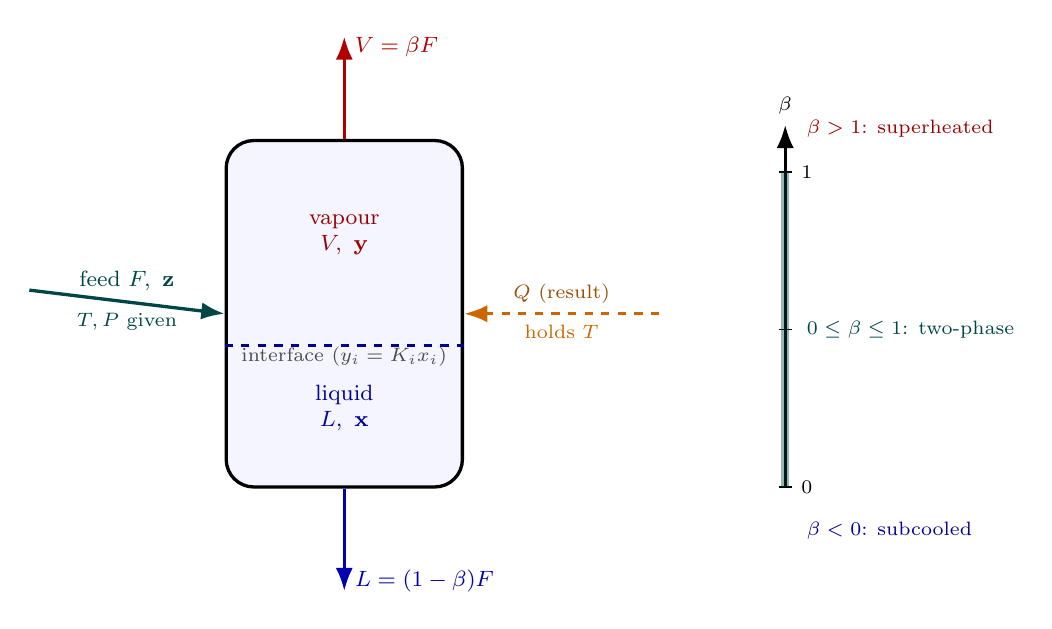
\begin{tikzpicture}[
    >={Latex[width=2.2mm]},
    every node/.style={font=\footnotesize},
    drum/.style={draw, very thick, rounded corners=10pt, fill=blue!4,
                 minimum width=30mm, minimum height=44mm},
    vap/.style={->, very thick, red!70!black},
    liq/.style={->, very thick, blue!70!black},
    feed/.style={->, very thick, teal!55!black},
    lbl/.style={font=\footnotesize, align=center},
]
% the drum body
\node[drum] (D) {};
% interface line (qualitative liquid level)
\draw[blue!55!black, very thick, dashed] (D.west|-0,-0.4) -- (D.east|-0,-0.4);
\node[lbl, blue!60!black] at (0,-1.2) {liquid\\ $L,\ \xv$};
\node[lbl, red!60!black]  at (0, 1.0) {vapour\\ $V,\ \yv$};
\node[font=\scriptsize, gray!60!black] at (0,-0.55) {interface ($y_i=K_i x_i$)};
% feed in from the left
\draw[feed] (-4.0,0.3) -- node[above]{feed $F,\ \zv$}
                          node[below, font=\scriptsize]{$T,P$ given} (D.west);
% vapour out the top
\draw[vap] (D.north) -- ++(0,1.3)
      node[right, pos=0.9]{$V=\beta F$};
% liquid out the bottom
\draw[liq] (D.south) -- ++(0,-1.3)
      node[right, pos=0.9]{$L=(1-\beta)F$};
% the heat-duty stub (a result, not an input)
\draw[->, very thick, orange!80!black, dashed]
      (4.0,0) -- node[above, orange!60!black, font=\scriptsize]{$Q$ (result)}
                  node[below, font=\scriptsize]{holds $T$} (D.east);
% the regime ruler on the right
\begin{scope}[shift={(5.6,-2.2)}]
  \draw[very thick, ->] (0,0) -- (0,4.6) node[above, font=\scriptsize]{$\beta$};
  \foreach \y/\t in {0/0,2/{\;}, 4/1}
     \draw (-0.08,\y) -- (0.08,\y) node[right, font=\scriptsize]{$\t$};
  \draw[blue!70!black, line width=2pt] (0,-0.0) -- (0,0.0);
  \node[font=\scriptsize, blue!60!black, anchor=west] at (0.15,-0.55)
        {$\beta<0$: subcooled};
  \node[font=\scriptsize, teal!55!black, anchor=west] at (0.15,2.0)
        {$0\le\beta\le1$: two-phase};
  \node[font=\scriptsize, red!60!black, anchor=west] at (0.15,4.55)
        {$\beta>1$: superheated};
  \draw[teal!50!black, line width=3pt, opacity=0.4] (0,0) -- (0,4);
\end{scope}
\end{tikzpicture}
\caption{The flash drum as hardware.  One feed $(F,\zv)$ at the
specified $(T,P)$ enters and disengages into a vapour $V=\beta F$ off the
top and a liquid $L=(1-\beta)F$ off the bottom, the two phases meeting at
the interface where $y_i=K_i x_i$.  The vapour fraction $\beta=V/F$ is
\emph{not} an input --- it is the Rachford--Rice root forced by the mass
balance.  The duty $Q$ (dashed, orange) is whatever heat must cross the
wall to \emph{hold} $T$ while part of the feed changes phase: a
\emph{result} of the converged energy balance, shown as a stream, never a
hidden number.  The ruler on the right reads $\beta$ back as a regime
tag: a $\beta$ outside $[0,1]$ is the honest signal that the feed is
single-phase (subcooled or superheated) at the chosen $T,P$.}
\label{fig:flash-drum}
\end{figure}


\begin{whatyoulllearn}
The end-to-end algorithm the simulator runs for a V-L flash: outer
Wegstein loop on $\gamma$, inner Newton on $\beta$, exit conditions and
diagnostics.
\end{whatyoulllearn}

\subsection{Problem statement}

\textbf{Given}: $\zv$, $T$, $P$, a thermo package (Antoine,
activity model). \\
\textbf{Find}: $\beta$, $\xv$, $\yv$ such that
\eqref{eq:K-modified-raoult} and \eqref{eq:RR} hold simultaneously.

\subsection{Degrees of freedom: what you specify, what the flash computes}

A flash vessel takes \emph{one} feed and splits it, at equilibrium, into a
vapour and a liquid product.  Counting variables against equations tells you
exactly how many numbers the engineer must fix --- and which ones the simulator
is then free to move.  This is the single most common point of confusion, so we
spell it out.

\paragraph{The feed is given, not a degree of freedom.}  Its total flow $F$,
composition $\zv$ (with $\sum_i z_i = 1$, hence $C-1$ independent mole
fractions), and thermal state all arrive on the inlet stream.  Nothing about
the feed is yours to choose at the flash --- it is whatever the upstream unit
delivers.

\paragraph{With the feed fixed, exactly two degrees of freedom remain.}  The
unknowns of the split are $\{\beta,\ \xv,\ \yv,\ T,\ P,\ Q\}$.  Against them
stand the equilibrium relations $y_i = K_i x_i$, the $C$ component balances
$z_i = \beta\, y_i + (1-\beta)\, x_i$, the summation condition
$\sum_i x_i = \sum_i y_i$ (the Rachford-Rice constraint), and the energy balance
$Q = H_{\text{out}} - H_{\text{in}}$.  The bookkeeping leaves \emph{two} free.
This is \emph{Duhem's theorem}: the equilibrium state of a closed system of known
overall composition is fixed by exactly two independent variables, regardless of
how many components or phases are present.  (Equivalently via Gibbs' phase rule: a
two-phase $C$-component system has $\mathcal F = C - 2 + 2 = C$ intensive degrees
of freedom; the feed composition consumes $C-2$ of them through the lever rule,
leaving two.)  You close those two by specifying \emph{any two} of:

\begin{center}
\begin{tabular}{ll}
\toprule
\textbf{You specify} & \textbf{Flash type} \\
\midrule
$T$ and $P$       & \emph{isothermal} flash --- Choupo's \code{isothermalFlash} \\
$Q$ and $P$       & \emph{adiabatic} ($Q=0$) or fixed-duty flash; $T$ is found \\
$\beta$ and $P$   & fixed vapour fraction ($V/F$); $T$ is found \\
\bottomrule
\end{tabular}
\end{center}

\begin{figure}[ht]
\centering
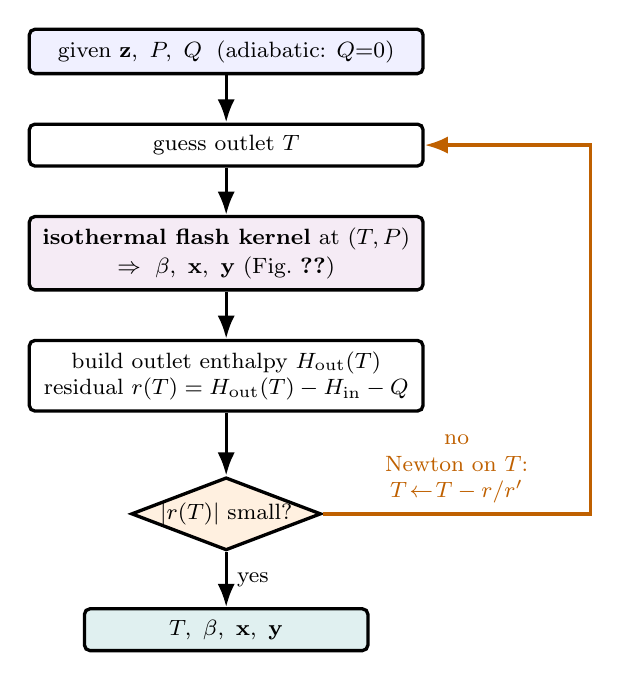
\begin{tikzpicture}[
    >={Latex[width=2.2mm]},
    every node/.style={font=\footnotesize},
    box/.style ={draw, rounded corners=2pt, very thick, align=center,
                 inner sep=4pt, minimum width=50mm},
    io/.style  ={draw, very thick, fill=blue!6, align=center, inner sep=4pt,
                 minimum width=50mm, rounded corners=2pt},
    inner/.style={draw, rounded corners=2pt, very thick, align=center,
                 inner sep=4pt, fill=violet!8, minimum width=50mm},
    test/.style={draw, diamond, aspect=2.6, very thick, fill=orange!12,
                 align=center, inner sep=0pt},
    done/.style={draw, rounded corners=2pt, very thick, fill=teal!12,
                 align=center, inner sep=4pt, minimum width=36mm},
    flow/.style={->, very thick},
    oloop/.style={->, very thick, orange!75!black},
]
\node[io]   (in)   {given $\zv,\ P,\ Q$ \;(adiabatic: $Q{=}0$)};
\node[box,  below=6mm of in]   (Tg)   {guess outlet $T$};
\node[inner, below=6mm of Tg]  (iso)  {\textbf{isothermal flash kernel} at $(T,P)$\\[1pt]
        $\Rightarrow\ \beta,\ \xv,\ \yv$ (Fig.~\ref{fig:flash-drum})};
\node[box,  below=6mm of iso]  (H)    {build outlet enthalpy $H_{\mathrm{out}}(T)$\\
        residual $r(T)=H_{\mathrm{out}}(T)-H_{\mathrm{in}}-Q$};
\node[test, below=8mm of H]    (conv) {$|r(T)|$ small?};
\node[done, below=7mm of conv] (out)  {$T,\ \beta,\ \xv,\ \yv$};
\draw[flow] (in)  -- (Tg);
\draw[flow] (Tg)  -- (iso);
\draw[flow] (iso) -- (H);
\draw[flow] (H)   -- (conv);
\draw[flow] (conv) -- node[right]{yes} (out);
\draw[oloop] (conv.east) -- ++(3.4,0)
      node[midway, above, align=center]{no\\ Newton on $T$:\\ $T\!\leftarrow\!T-r/r'$}
      |- (Tg.east);
\end{tikzpicture}
\caption{The adiabatic (or fixed-duty) flash is the isothermal flash
wearing one more loop.  Here $T$ is \emph{not} given --- the spec is the
duty $Q$ (zero for a true adiabatic throttle) and the pressure $P$.  The
outer Newton (orange) searches for the outlet temperature: at each trial
$T$ it runs the \emph{whole} isothermal kernel of
Fig.~\ref{fig:flash-drum} (itself two loops) to get the split, builds the
outlet enthalpy $H_{\mathrm{out}}(T)$, and forms the energy residual
$r(T)=H_{\mathrm{out}}(T)-H_{\mathrm{in}}-Q$.  Newton on $T$ drives $r$
to zero --- the temperature at which the phase split absorbs exactly the
specified duty.  The same kernel, reused: an isothermal flash fixes $T$
and \emph{reports} $Q$; the adiabatic flash fixes $Q$ and \emph{finds}
$T$.  This is Duhem's two degrees of freedom, closed from the other
side.}
\label{fig:adiabatic-flash-loops}
\end{figure}


\paragraph{Specified vs.\ manipulated, for the isothermal flash.}  In the
\code{operation} block you \textbf{specify} $T$ and $P$.  The simulator then
\textbf{manipulates} the remaining unknowns until every equation holds:

\begin{itemize}[leftmargin=*,nosep]
  \item the vapour fraction $\beta = V/F$ (the root of Rachford-Rice),
  \item the phase compositions $\xv$ and $\yv$,
  \item the heat duty $Q$ that must cross the boundary to \emph{hold} $T$
        constant while part of the feed changes phase --- read off the
        converged energy balance, $Q = H_{\text{out}} - H_{\text{in}}$.  On the
        flowsheet this $Q$ appears as the heat \emph{stream} feeding the unit
        (a docked utility stub + dashed wire), never as a hidden number.
\end{itemize}

\paragraph{Where the duty lives --- a flash \emph{gives} a $Q$, a heater
\emph{takes} one.}  Because $T,P$ already spend both degrees of freedom, $Q$ is a
\emph{result} of the isothermal flash, never an input --- the \code{operation}
block has no $Q$ key (it was removed on purpose).  The unit whose hardware knob
\emph{is} the duty is the \code{heater}: there you \textbf{specify} $Q$ and the
outlet $T$ is the result.  So ``inject a known $500\,$kW, then separate'' is a
\code{heater}$\,\to\,$\code{flash} chain (the heat enters on a visible wire), and
``hold the outlet at a target $T$'' is a \emph{design spec} that manipulates the
heater's $Q$ in a visible outer loop --- exactly as outlet pressure is handled on
a compressor (specify $W_{\text{shaft}}$, target $P_{\text{out}}$).  This is the
``heat is a stream, not a hidden number'' rule applied to the flash.

\begin{intuition}
The trap is to count $T$, $P$ \emph{and} $\beta$ as three inputs.  Once $T$ and
$P$ are set, $\beta$ is \emph{not} free --- it is whatever the two-phase mass
balance forces, and it may even land outside $[0,1]$ (subcooled liquid or
superheated vapour, see the regime tags below).  Symmetrically, the duty $Q$ is
\emph{never} specified for an isothermal flash; it is the answer, not the
question.  Pick the two specifications that match the equipment: a flash drum
held by a thermostat is $T,P$; an adiabatic throttle is $Q{=}0,P$; a partial
condenser sized for a target recovery is $\beta,P$.
\end{intuition}

\subsection{Algorithm}

\begin{enumerate}[leftmargin=*,nosep,topsep=2pt]
  \item Initialise $\Kv$ from Wilson \eqref{eq:wilson-K}.
  \item Solve Rachford-Rice \eqref{eq:RR} for $\beta$ by Newton-1D.
  \item Compute $\xv, \yv$ from \eqref{eq:xy-from-K}.
  \item Compute $\boldsymbol{\gamma}^{(k+1)} = \gamma(\xv, T)$.
  \item Update $K_i = \gamma_i \, \Psat_i(T) / P$.
  \item Wegstein-accelerate $\Kv$ (component-wise; \eqref{eq:wegstein}).
  \item If $\|\Kv^{(k+1)} - \Kv^{(k)}\|_\infty < \varepsilon$, exit; else goto 2.
\end{enumerate}

% --- Figure: the two-loop isothermal flash ---------------------------
\begin{figure}[h]
\centering
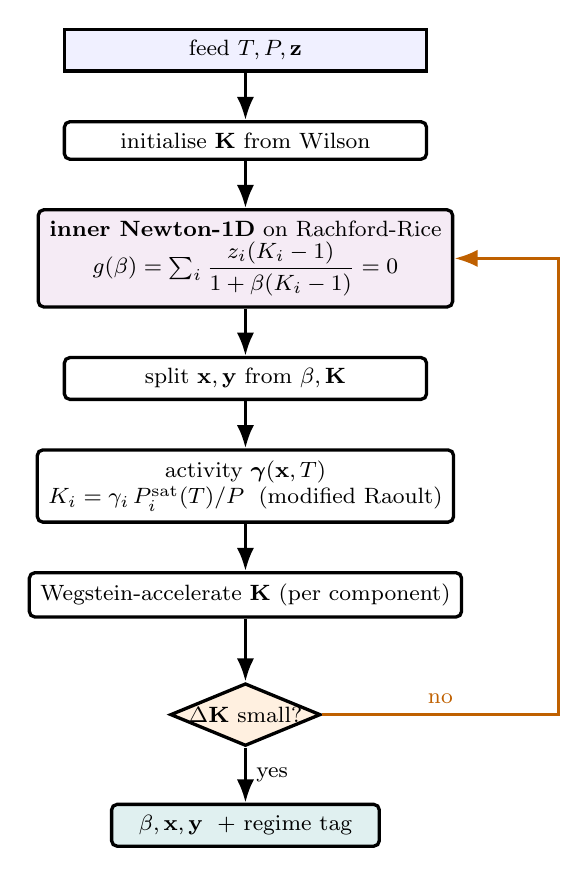
\begin{tikzpicture}[
    >={Latex[width=2.2mm]},
    every node/.style={font=\footnotesize},
    box/.style ={draw, rounded corners=2pt, very thick, align=center,
                 inner sep=4pt, minimum width=46mm},
    io/.style  ={draw, very thick, fill=blue!6, align=center, inner sep=4pt,
                 minimum width=46mm},
    inner/.style={draw, rounded corners=2pt, very thick, align=center,
                 inner sep=4pt, fill=violet!8, minimum width=46mm},
    test/.style={draw, diamond, aspect=2.4, very thick, fill=orange!12,
                 align=center, inner sep=0pt},
    done/.style={draw, rounded corners=2pt, very thick, fill=teal!12,
                 align=center, inner sep=4pt, minimum width=34mm},
    flow/.style={->, very thick},
    iloop/.style={->, very thick, violet!70!black},
    oloop/.style={->, very thick, orange!75!black},
]
\node[io]   (in)   {feed $T,P,\zv$};
\node[box,  below=6mm of in]  (Kinit) {initialise $\Kv$ from Wilson};
\node[inner, below=6mm of Kinit] (rr)   {\textbf{inner Newton-1D} on Rachford-Rice\\[1pt]
        $g(\beta)=\sum_i\dfrac{z_i(K_i-1)}{1+\beta(K_i-1)}=0$};
\node[box,  below=6mm of rr]   (xy)    {split $\xv,\yv$ from $\beta,\Kv$};
\node[box,  below=6mm of xy]   (gam)   {activity $\boldsymbol\gamma(\xv,T)$\\
        $K_i=\gamma_i\,\Psat_i(T)/P$ \;(modified Raoult)};
\node[box,  below=6mm of gam]  (weg)   {Wegstein-accelerate $\Kv$ (per component)};
\node[test, below=8mm of weg]  (conv)  {$\Delta\Kv$ small?};
\node[done, below=7mm of conv] (out)   {$\beta,\xv,\yv$ \;+ regime tag};
\draw[flow] (in)    -- (Kinit);
\draw[flow] (Kinit) -- (rr);
\draw[flow] (rr)    -- (xy);
\draw[flow] (xy)    -- (gam);
\draw[flow] (gam)   -- (weg);
\draw[flow] (weg)   -- (conv);
\draw[flow] (conv)  -- node[right]{yes} (out);
% outer loop back to Rachford-Rice with the updated K
\draw[oloop] (conv.east) -- ++(3.0,0)
             node[midway, above]{no}
             |- (rr.east);
\end{tikzpicture}
\caption{The isothermal V--L flash is \emph{two nested loops}.  The
\textbf{inner} loop (violet) is a Newton-1D that solves the
Rachford--Rice equation for the vapour fraction $\beta$ at the current
$K$-values --- a clean monotone root.  The \textbf{outer} loop (orange)
updates the $K$-values: from the trial split it re-evaluates the
activity coefficients $\gamma_i(\xv,T)$, rebuilds $K_i=\gamma_i\Psat_i/P$
through modified Raoult, and Wegstein-accelerates them.  When the
$K$-values stop moving the two loops are mutually consistent and the
flash is converged; the final $\beta$ also classifies the regime
(subcooled $\beta<0$, two-phase $0\le\beta\le1$, superheated
$\beta>1$).  For an \emph{ideal} system the activity step is a no-op and
only the inner loop runs once --- the same code, fewer passes.}
\label{fig:flash-two-loops}
\end{figure}

\subsection{Diagnostics in the log}

At \code{verbosity 3}, the simulator prints:

\begin{itemize}[leftmargin=*,nosep]
  \item Inner Newton trace on Rachford-Rice:
        $(\beta^{(j)}, g(\beta^{(j)}), g'(\beta^{(j)}))$ per iteration.
  \item Outer Wegstein trace: $\gamma_i^{(k)}$ and $q_i^{(k)}$ per component.
  \item Final regime tag: \code{V-L (subcooled)} if $\beta < 0$,
        \code{V-L (superheated)} if $\beta > 1$, \code{V-L (two-phase)}
        otherwise.
\end{itemize}

\begin{intuition}
The most informative number to watch is $q_i^{(k)}$. If $q$ sits near
$q_{\min}$, the system is strongly non-linear (azeotrope nearby) and
the simulator is choosing the most aggressive accepted extrapolation.
If $q \approx 0$, the system is mildly non-linear and direct
substitution would have been fine.
\end{intuition}

% ---------------------------------------------------------------------
\section{Phase changer: the dome-crossing boiler / condenser}\label{ch:phase-changer}

\begin{whatyoulllearn}
How Choupo's \code{phaseChanger} (and its aliases \code{boiler} and
\code{condenser}) takes one stream across the saturation dome --- subcooled
liquid, anywhere inside the two-phase region, or superheated vapour --- by
specifying \emph{one} outlet coordinate and letting the heat duty $Q$ fall out
as the result.  How the saturation temperature is read off $\Psat$ (or an IF97
$T^{\mathrm{sat}}(P)$ kernel for a pure fluid), how the latent/sensible split is
recovered, and why ``boiler'' and ``condenser'' are not separate models but
emergent labels.
\end{whatyoulllearn}

\subsection{Where it sits between a heater and a flash}

\begin{figure}[ht]
\centering
\begin{tikzpicture}[
    >={Latex[width=2.2mm]},
    every node/.style={font=\footnotesize},
    unit/.style={draw, rounded corners=2pt, very thick, align=center,
                 inner sep=4pt, minimum width=30mm, minimum height=13mm},
    spec/.style={font=\scriptsize, align=center},
    fl/.style={->, very thick},
]
\node[unit, fill=blue!10] (heater) {\textbf{heater}\\{\scriptsize you give $Q$ (duty)}};
\node[unit, fill=orange!12, right=16mm of heater] (phase)
     {\textbf{phase changer}\\{\scriptsize cross the dome to a}\\
      {\scriptsize target $V/F$ or $T$}};
\node[unit, fill=teal!12, right=16mm of phase] (flash)
     {\textbf{flash}\\{\scriptsize you give $T,P$;}\\
      {\scriptsize split is a result}};
\draw[fl] (heater) -- (phase);
\draw[fl] (phase) -- (flash);
% the duty/state contrast underneath
\node[spec, below=6mm of heater, blue!70!black]
     {$Q$ in, $T_{\text{out}}$ out\\ (no phase split asked)};
\node[spec, below=6mm of phase, orange!85!black]
     {boil / condense to a\\ \emph{set} endpoint; $Q$ a result};
\node[spec, below=6mm of flash, teal!50!black]
     {2 of $\{T,P,Q,V/F\}$ fix it\\ (Duhem); $Q$ always a result};
% the spectrum arrow
\draw[->, gray, thick] ($(heater.north)+(0,0.6)$) -- ($(flash.north)+(0,0.6)$)
      node[midway, above, gray]
      {duty-driven \quad$\longrightarrow$\quad state-driven};
\end{tikzpicture}
\caption{Three single-vessel thermal units, ordered by what the student
specifies.  The \textbf{heater} is duty-driven: you furnish $Q$ and the
outlet temperature follows --- no phase split is even asked.  The
\textbf{flash} is state-driven: you fix two of $\{T,P,Q,V/F\}$ (Duhem's
rule), and the vapour--liquid split is the result, with $Q$ \emph{always}
an output, never an input key.  The \textbf{phase changer} sits between
them --- a boiler/condenser that crosses the saturation dome to a
\emph{set} endpoint (a target $V/F$ or $T$), reporting the duty it took.
Reading the units this way --- duty-driven on the left, state-driven on
the right --- keeps the degrees of freedom straight and avoids the
classic ``is $Q$ an input or an output?'' confusion.}
\label{fig:thermal-units-spectrum}
\end{figure}


A \code{heater} (Sec.~\ref{ch:simple-ops}) is \emph{sensible-only}: you give it a
duty $Q$, it returns the outlet $T$, and it must \emph{not} cross the saturation
line --- it refuses loudly if the energy you inject would start vaporising the
stream.  An \code{isothermalFlash} (Sec.~\ref{ch:flash}) fixes $T$ and $P$ and
\emph{reports} the duty $Q$ that holds $T$ while the feed splits.  The
\code{phaseChanger} is the unit built for the case in between: a piece of
hardware whose explicit \emph{job} is to land the outlet somewhere on the
$(T,\mathrm{vf})$ surface that the heater forbids and the isothermal flash cannot
target directly.  One stream in, one (two-phase-aware) stream out, $Q$ a result.

\subsection{Degrees of freedom: one outlet coordinate}

By Duhem's theorem (Sec.~\ref{ch:flash}) the outlet of a single feed at known
$\zv$ is fixed by exactly two numbers.  The \code{phaseChanger} spends the first
on pressure --- $P_{\mathrm{out}}$ is \emph{held} from the inlet unless you set
\code{P} explicitly --- and asks you to spend the second by picking
\textbf{exactly one} outlet coordinate:

\begin{center}
\begin{tabular}{lll}
\toprule
\textbf{You specify} & \textbf{Meaning} & \textbf{Result} \\
\midrule
\code{Q}             & duty added/removed (kW)            & $T_{\mathrm{out}},\ \mathrm{vf}_{\mathrm{out}}$ \\
\code{outletT}       & outlet temperature                 & $Q$ \\
\code{outletQuality} & target vapour fraction $\mathrm{vf}\in[0,1]$ & $Q$ \\
\code{outletState}   & \code{saturatedLiquid} / \code{saturatedVapour} & $Q$ \\
\code{superheat}     & $T = T^{\mathrm{sat}}(P)+\Delta K$ (vapour side) & $Q$ \\
\code{subcool}       & $T = T^{\mathrm{sat}}(P)-\Delta K$ (liquid side) & $Q$ \\
\bottomrule
\end{tabular}
\end{center}

Supplying zero or more than one coordinate is a hard error --- the
degree-of-freedom count is enforced, never silently patched.  Every mode but the
first is an inverse problem: the unit \emph{self-targets}, solving for the $Q$
that lands the outlet on the coordinate you declared, and \emph{announces} that
inverse solve in its report (the no-silent-crutch rule --- there is no hidden
\code{outerDict} or design-spec loop, the solve is built in but visible).  The
single-phase states \code{subcooledLiquid} / \code{superheatedVapour} are
refused as bare \code{outletState} words precisely because they need that extra
distance from saturation; you must give \code{subcool}/\code{superheat} instead.

\subsection{The saturation temperature}

Every spec mode needs the position of the dome at $P_{\mathrm{out}}$, i.e.\ the
saturation temperature $T^{\mathrm{sat}}(P)$.  Choupo locates it from the
\emph{dominant} component (the one with the largest mole fraction) by two routes:

\begin{itemize}[leftmargin=*,nosep]
  \item \textbf{Pure-fluid route.}  If the dominant species carries an IF97-class
        pure-fluid kernel \emph{and} the feed is effectively pure, the kernel's
        closed-form $T^{\mathrm{sat}}(P)$ is used directly.
  \item \textbf{Generic route.}  Otherwise the dominant component's vapour-pressure
        curve is inverted by bisection,
        \begin{equation}
          \Psat_{\mathrm{dom}}\!\big(T^{\mathrm{sat}}\big) = P_{\mathrm{out}},
          \label{eq:pc-tsat}
        \end{equation}
        over $T\in[150,1200]\,$K (the Antoine root, Sec.~\ref{ch:vap}).
\end{itemize}

For a \emph{pure} (or dominant-component) dome the saturation plateau is a single
$T = T^{\mathrm{sat}}$ and the vapour fraction $\mathrm{vf}$ is the free
coordinate along it: $H$ spans $[h_f,h_g]$ at \emph{constant} $T$.  For a genuine
multicomponent mixture the dome has \emph{width} in $T$ (the bubble-to-dew
interval), so $\mathrm{vf}(T)$ rises smoothly from 0 at the bubble point to 1 at
the dew point, and the engine brackets the sign-changing interval on a flash scan
before driving Newton inside it.  This split --- step-at-$T^{\mathrm{sat}}$ for a
pure dome, smooth-$\mathrm{vf}(T)$ for a mixture --- is the one subtlety that
distinguishes the two cases throughout the solve.

\subsection{Dome-aware enthalpy and the vf closure}

The whole unit is built on the existing flash kernel:
\code{IsothermalFlash::solveCore} returns the split $(\beta,\xv,\yv)$ at any
$(T,P_{\mathrm{out}})$, and the stream enthalpy is the lever-rule blend of the
equilibrium phases,
\begin{equation}
  H(T,P) \;=\; (1-\beta)\,h_f(\xv,T,P) \;+\; \beta\,h_g(\yv,T,P),
  \label{eq:pc-Hstream}
\end{equation}
the very enthalpies the produced liquid and vapour streams carry.  The molar
latent heat at saturation is $h_g - h_f$.

\paragraph{The vf=1 trap, and the $\varepsilon$-step that avoids it.}  Evaluating
the enthalpy at \emph{exactly} $\mathrm{vf}=1$ on the saturation line is
dangerous: at $P = \Psat$ the property routing falls onto the \emph{liquid}
branch (region~1 of an IF97 kernel; the single-phase side of a cubic EoS) and
silently \emph{loses the latent heat}.  Choupo therefore probes a tiny step
$\varepsilon = 10^{-4}$ \emph{into} the two-phase region and extrapolates the
endpoints linearly back out:
\begin{align}
  h_{\mathrm{lo}} &= H(T^{\mathrm{sat}},P,\ \varepsilon),
  & h_{\mathrm{hi}} &= H(T^{\mathrm{sat}},P,\ 1-\varepsilon), \nonumber\\
  h_f &= \frac{h_{\mathrm{lo}} - \varepsilon\,h_{\mathrm{hi}}}{1-2\varepsilon},
  & h_g &= \frac{h_{\mathrm{hi}} - \varepsilon\,h_{\mathrm{lo}}}{1-2\varepsilon}.
  \label{eq:pc-hfhg}
\end{align}
This recovers the true $h_f,h_g$ (hence the latent heat) without ever asking the
thermo for an ambiguous on-line point.

\paragraph{Duty mode --- closing on $\mathrm{vf}$.}  In duty mode you give $Q$;
the target outlet enthalpy is
\begin{equation}
  H_{\mathrm{target}} \;=\; H_{\mathrm{in}} \;+\; \frac{Q}{F\,},
  \label{eq:pc-Htarget}
\end{equation}
($F$ in mol\,s$^{-1}$, $Q$ in W).  On a pure dome the engine first tests whether
$H_{\mathrm{target}}$ falls on the plateau, $h_f \le H_{\mathrm{target}} \le
h_g$; if so the outlet sits at $T^{\mathrm{sat}}$ and the vapour fraction is read
straight off the lever rule,
\begin{equation}
  \mathrm{vf}_{\mathrm{out}} \;=\;
     \frac{H_{\mathrm{target}} - h_f}{h_g - h_f},
  \label{eq:pc-lever}
\end{equation}
clipped to $[0,1]$.  Only \emph{outside} the plateau --- where $H(T)$ is smooth
and monotone --- does a single Newton-on-$T$ run, with the pure-fluid kernel's
triple-point floor ($T \ge 274\,$K) protecting the search from the kernel's
forbidden region.  A multicomponent dome has no plateau, so duty mode Newtons on
$T$ throughout.

\subsection{The duty is always a result; latent / sensible split}

Whatever coordinate you picked, the duty is computed last, from the converged
endpoints:
\begin{equation}
  Q \;=\; F\,\big(H_{\mathrm{out}} - H_{\mathrm{in}}\big),
  \qquad Q>0\ \text{added},\quad Q<0\ \text{removed}.
  \label{eq:pc-duty}
\end{equation}
It is reported as \code{DUTY (result)} and, on the flowsheet, appears as a heat
\emph{stream} (a utility stub + dashed wire), never as a number painted on the
node.  Choupo further attributes the duty to a \emph{latent} share --- the part
tied to the change in vapour fraction at saturation --- and a \emph{sensible}
remainder:
\begin{equation}
  Q_{\mathrm{latent}} \;=\; F\,\big(\mathrm{vf}_{\mathrm{out}} - \mathrm{vf}_{\mathrm{in}}\big)\,(h_g - h_f),
  \qquad
  Q_{\mathrm{sensible}} \;=\; Q - Q_{\mathrm{latent}},
  \label{eq:pc-latent}
\end{equation}
with $h_g - h_f$ the latent heat from \eqref{eq:pc-hfhg} at $T^{\mathrm{sat}}$.

\subsection{Boiler and condenser are emergent labels}

There is \emph{one} class.  After convergence Choupo reads the sign of $Q$ and
the outlet vapour fraction and prints a \emph{role}: a positive duty landing on
saturated vapour is a \code{boiler}, partway up the dome a \code{partial boiler};
a negative duty landing on saturated liquid is a \code{condenser}, partway down a
\code{partial condenser}; a duty that stays single-phase is just a heater/cooler.
The aliases \code{boiler} and \code{condenser} register the \emph{same} class ---
the direction is emergent from the physics, not a model switch, so a case that
mis-labels a condensing duty as a \code{boiler} still computes the correct
(negative) $Q$ and says so.

\begin{example}[Saturated-vapour boiler on a pure dome]
Feed: saturated-or-subcooled water at $P=1\,$bar, $F=1\,$kmol\,s$^{-1}$, with
\code{outletState saturatedVapour;}.  The engine finds
$T^{\mathrm{sat}}(1\,\text{bar})\approx 372.8\,$K from the pure-fluid kernel, sets
$T_{\mathrm{out}}=T^{\mathrm{sat}}$ and forces $\mathrm{vf}_{\mathrm{out}}=1$ (vf
is the free coordinate on the plateau).  With $H_{\mathrm{out}}=h_g$ and
$H_{\mathrm{in}}=h_f$ the latent heat $h_g-h_f\approx 40.7\,$kJ\,mol$^{-1}$ gives
$Q = F(h_g-h_f)\approx 1000\cdot 40.7 = 4.07\times10^{4}\,$kW, reported as a
positive duty, role \code{boiler}, $Q_{\mathrm{latent}}\approx Q$ and
$Q_{\mathrm{sensible}}\approx 0$.  Re-specify \code{outletQuality 0.5;} and the
same plateau gives half the latent duty.
\end{example}

\paragraph{Power and limit.}  \textbf{Power:} one class spans every dome-crossing
service with a single, honest degree of freedom; the duty is always a visible
result; the latent/sensible split and the boiler/condenser role come for free
from the converged state; and the same code path serves both the generic
cubic-EoS\,+\,Antoine route and the high-accuracy pure-fluid (IF97) route, the
dispatch hidden inside the thermo.  \textbf{Limit:} the saturation dome is
located from the \emph{dominant} component, so the single $T^{\mathrm{sat}}$ used
for the latent split is a pure/dominant-component approximation --- for a wide
multicomponent dome it is only the bracket centre, and a strongly non-ideal
mixture's true bubble-to-dew width is captured by the flash but not by that one
plateau temperature.  The unit is a thermodynamic phase-change \emph{specifier},
not a rating model: it does not size area or compute a real heat-transfer
coefficient unless you switch to \code{model geometry;} (the Nusselt
film-condensation / Rohsenow nucleate-boiling branch with a Zuber CHF ceiling),
documented in the heat-transfer rating material.

\medskip\noindent
\emph{Primary references:} the saturation curve and Clausius--Clapeyron latent
heat (Sec.~\ref{ch:vap}); Smith, Van Ness \& Abbott, \emph{Introduction to
Chemical Engineering Thermodynamics}, on the lever rule and dome enthalpies; IAPWS
R7-97 (IF97) for the pure-fluid $T^{\mathrm{sat}}(P)$ kernel; for the geometry
branch, Nusselt (1916) film condensation and Rohsenow (1952) / Zuber (1959)
nucleate boiling and critical heat flux.

% ---------------------------------------------------------------------
\section{Continuous stirred-tank reactor (CSTR)}\label{ch:cstr}

\begin{whatyoulllearn}
A single-reaction steady-state CSTR collapses to a one-dimensional
Newton solve in the reaction extent $\xi$. The simulator does exactly
that.
\end{whatyoulllearn}

\subsection{Material balance with reaction extent}

For one independent reaction with stoichiometry $\boldsymbol\nu$ and
rate $r(\xv, T)$ (units mol/(m\textsuperscript{3}\,s)), the steady-state
component balance over the reactor is
\begin{equation}
   F_{\mathrm{in}}\,\zv_{\mathrm{in}}
   \;=\; F_{\mathrm{out}}\,\zv_{\mathrm{out}}
   \;-\; V_R \, \boldsymbol\nu \, r(\zv_{\mathrm{out}}, T).
\end{equation}
Using the extent of reaction $\xi$ (mol/h) we write
$\zv_{\mathrm{out}} F_{\mathrm{out}} = \zv_{\mathrm{in}} F_{\mathrm{in}}
 + \boldsymbol\nu \, \xi$. Eliminating $\zv_{\mathrm{out}}$:
\begin{equation}
   g(\xi) \;\equiv\; \xi - V_R\,r\bigl(\zv_{\mathrm{out}}(\xi), T\bigr) \;=\; 0.
   \label{eq:cstr}
\end{equation}

\begin{figure}[ht]
\centering
\begin{tikzpicture}[
    >={Latex[width=2.2mm]},
    every node/.style={font=\footnotesize},
    box/.style={draw, rounded corners=2pt, very thick, align=center,
                inner sep=4pt, minimum width=30mm, minimum height=9mm},
    dec/.style={draw, very thick, fill=orange!12, align=center,
                inner sep=3pt, minimum width=26mm},
    fl/.style={->, very thick},
]
\node[box, fill=blue!10] (init) {guess $\xi^{(0)}=0$};
\node[box, below=7mm of init] (comp) {rebuild outlet\\
      $\zv_{\text{out}}(\xi)=\zv_{\text{in}}+\boldsymbol\nu\,\xi/F$};
\node[box, below=6mm of comp] (res) {residual\\
      $g(\xi)=\xi-V_R\,r(\zv_{\text{out}},T)$};
\node[dec, below=6mm of res] (chk) {$|g|<\epsilon$?};
\node[box, below=7mm of chk, fill=teal!12] (done) {outlet stream\\
      $F\,\zv_{\text{out}}$};
\node[box, right=16mm of res] (upd) {Newton step\\
      $\xi\leftarrow\xi-g/g'$};
\draw[fl] (init) -- (comp);
\draw[fl] (comp) -- (res);
\draw[fl] (res) -- (chk);
\draw[fl] (chk) -- node[right]{yes} (done);
\draw[fl] (chk.east) -- node[above]{no} ++(2.0,0) |- (upd.east);
\draw[fl] (upd) -- (comp.east);
\end{tikzpicture}
\caption{The steady CSTR is \emph{not} a big system --- it collapses to
one scalar root-find.  The single unknown is the reaction extent $\xi$;
every outlet mole fraction is rebuilt from it through stoichiometry
$\zv_{\text{out}}=\zv_{\text{in}}+\boldsymbol\nu\,\xi/F$, the rate
$r(\zv_{\text{out}},T)$ is evaluated there, and the residual
$g(\xi)=\xi-V_R r$ measures how far the guessed extent is from
production-equals-consumption.  A damped \textbf{Newton-1D} (right
loop) drives $g\to0$ in 3--5 iterations.  The whole reactor is one
equation in one number.}
\label{fig:cstr-newton-loop}
\end{figure}

A single non-linear equation in a single unknown $\xi$: \textbf{Newton-1D
in one variable}, with damping. Convergence is typically 3--5 iterations.

\subsection{First-order kinetics --- analytic check}

For an Arrhenius first-order reaction $r = k\, c_A$ with
$k = k_0\, e^{-E_a / \Rgas T}$, the steady-state CSTR has the
analytic solution
\begin{equation}
   X_A \;\equiv\; 1 - \frac{c_A}{c_{A,0}} \;=\; \frac{\mathrm{Da}}{1 + \mathrm{Da}},
   \qquad \mathrm{Da} = k\,\tau,
\end{equation}
where $\tau = V_R / Q$ is the residence time. The simulator reproduces
this to machine precision in \code{tutorials/cstr01\_first\_order}.

\subsection{Worked example}

\begin{example}[First-order $A \to B$ in a 0.5\,m\textsuperscript{3} CSTR]
Inlet: $c_{A,0} = 100$ mol/m\textsuperscript{3}, volumetric flow $Q = 0.01$
m\textsuperscript{3}/s, kinetic constant $k = 0.02$ s\textsuperscript{-1}.
Then $\tau = V_R / Q = 50$\,s, $\mathrm{Da} = 1.0$, $X_A = 0.5$. Newton
starting from $\xi^{(0)} = 0$ converges in 4 iterations to
$\xi = 0.5\,c_{A,0}\,Q = 0.5$ mol/s.
\end{example}

\begin{tutoriallink}
\file{tutorials/cstr01\_first\_order} --- includes the analytic check in
the case output.
\end{tutoriallink}

% ---------------------------------------------------------------------
\section{The rate law: from mass action to
Langmuir--Hinshelwood}\label{ch:lhhw}

\begin{whatyoulllearn}
Why a power law cannot describe a catalytic reaction at any order, where the
denominator of an LHHW rate law comes from, and why a rate constant means nothing
without the rate law and the activity model it was regressed with.
\end{whatyoulllearn}

Every reactor so far has been handed a rate $r(\mathbf{c}, T)$ and asked what to do with
it: a CSTR sets $\xi = r V_R$, a PFR integrates it along the volume, a batch
vessel integrates it in time.  None of them cares what $r$ is.  This section is
about $r$ itself, and in Choupo it is one object --- the shared \code{RateLaw} ---
so a batch vessel and a continuous one cannot disagree about it.

\subsection{Where mass action stops}

For a homogeneous elementary step the rate is a product of concentrations raised
to the stoichiometric orders: mass action, the law of a well-mixed molecular
collision.  A \emph{catalytic} reaction is not that.  The molecules do not meet in
the fluid; they meet on a surface, and the surface has a finite number of sites.

Follow Langmuir.  Let $\theta_i$ be the fraction of sites carrying species $i$ and
$\theta_v$ the fraction left vacant.  Adsorption and desorption of $i$ balance at
equilibrium,
\[
k_{a,i}\, c_i\, \theta_v \;=\; k_{d,i}\, \theta_i
\qquad\Longrightarrow\qquad
\theta_i \;=\; K_i\, c_i\, \theta_v ,
\]
with $K_i = k_{a,i}/k_{d,i}$ the \emph{adsorption equilibrium constant} of $i$.
Every site is either vacant or occupied, so $\theta_v + \sum_i \theta_i = 1$ and
therefore
\begin{equation}
\theta_v \;=\; \frac{1}{1 + \sum_i K_i c_i} ,
\qquad
\theta_i \;=\; \frac{K_i c_i}{1 + \sum_i K_i c_i} .
\label{eq:langmuir}
\end{equation}

Now let the rate-determining step be a surface reaction between adsorbed species.
Its rate is proportional to the coverages of the reactants --- not to their bulk
concentrations --- so for a bimolecular step $A_{\mathrm{ads}} + B_{\mathrm{ads}}$
occupying two sites,
\begin{equation}
r \;=\; k\,\theta_A\,\theta_B
  \;=\; \frac{k\,K_A c_A\, K_B c_B}{\bigl(1 + \sum_i K_i c_i\bigr)^{2}} .
\label{eq:lhhw-canonical}
\end{equation}

That denominator is the whole point, and no power law contains it.  Look at what
it does.  A \emph{product} that adsorbs strongly appears in $\sum_i K_i c_i$ but
not in the numerator: as the reaction makes it, it covers the surface, crowds the
reactants off, and \textbf{throttles the reaction that produced it}.  This is
product inhibition.  You cannot reproduce it by tuning the order of a power law,
because a power law's dependence on a product's concentration is monotone in one
direction only.  Equation~\eqref{eq:lhhw-canonical} is the
Langmuir--Hinshelwood--Hougen--Watson (LHHW) form \cite{Langmuir1918,
Hinshelwood1940, HougenWatson1943}.

\subsection{The one formula Choupo evaluates}

Choupo does not carry a taxonomy of LHHW shapes.  It carries one expression, and
the shapes are what you get by choosing its parts.  Write $\theta_i$ for the
intensive variable of species $i$ --- a concentration, or an \emph{activity}
$a_i = \gamma_i x_i$ when \code{basis activity} --- and weight it by its adsorption
constant to get the species \emph{as the surface sees it},
\[
\bar a_i \;=\; K_i(T)\,\theta_i ,
\qquad K_i(T) = K^0_i\,\mathrm{e}^{B_i/T}
\]
($B_i$ the van 't Hoff slope; $K_i = 1$ for a species that declares no
adsorption).  Then
\begin{equation}
\boxed{\;
r \;=\;
\frac{k_f \prod_i \bar a_i^{\,\alpha_i}
      \;-\; k_r \prod_i \bar a_i^{\,\beta_i}}
     {\bigl(v + \sum_{i \in \mathrm{ads}} \bar a_i\bigr)^{p}}
\;}
\label{eq:ratelaw}
\end{equation}

Three dials, and every rate law in this guide is a setting of them.

\begin{itemize}
\item $p = 0$ (no \code{adsorption} block): the denominator is $1$ and what
      remains is the plain power law, \code{type Arrhenius}.  Mass action.
\item $p > 0$: LHHW.  The exponent is the number of sites the rate-determining
      step occupies --- $p=2$ in Eq.~\eqref{eq:lhhw-canonical}.
\item $v$ is the vacant-site term.  It is $1$ in the classical Hougen--Watson
      forms, and $0$ where the surface is taken as saturated --- an ion-exchange
      resin swollen with liquid, say, on which every site holds \emph{something}
      and only the competition matters.
\end{itemize}

Note that $\bar a_i$ sits in the numerator too.  That is not a convention: the
rate-determining surface step sees the \emph{adsorbed} species, as
Eq.~\eqref{eq:lhhw-canonical} shows.  Any constant $K_i$ can of course be absorbed
into $k_f$, which is exactly why textbook LHHW forms look different from one
another --- and it is the first hint of the pitfall below.

The reverse leg is either \textbf{detailed balance} (\code{reversible true}:
$k_r = k_f/K_c$, so equilibrium sits precisely where the thermodynamics puts it,
and cannot drift with a fitted number), or an \textbf{explicitly regressed}
Arrhenius pair $(k_r^0, E_{a,r})$ --- which is what a kinetics paper reports.
Choupo refuses both at once, and refuses detailed balance on an activity basis,
since $K_c$ is a concentration-basis constant.

\subsection{Per gram of catalyst}

A heterogeneous rate constant is reported per gram of dry catalyst, and a reactor
is measured in cubic metres.  Declare the bulk loading $\rho_{\mathrm{cat}}$ and
the conversion is exact:
\[
r\;\Bigl[\tfrac{\mathrm{kmol}}{\mathrm{m^3\,s}}\Bigr]
\;=\; \rho_{\mathrm{cat}}\Bigl[\tfrac{\mathrm{kg}}{\mathrm{m^3}}\Bigr]
      \cdot r\Bigl[\tfrac{\mathrm{mol}}{\mathrm{g\,s}}\Bigr] .
\]
It is a declared, printed number --- change the packing and the reactor changes
with it.

\subsection{A worked, cited example, and a trap}

Methyl-acetate synthesis over the ion-exchange resin Amberlyst~15,
$\mathrm{CH_3OH} + \mathrm{CH_3COOH} \rightleftharpoons
 \mathrm{CH_3COOCH_3} + \mathrm{H_2O}$, follows Eq.~16 of P\"opken, G\"otze and
Gmehling \cite{Popken2000} --- the adsorption-based model the authors recommend
(mean relative error $5.4\,\%$, against $13.9\,\%$ for the pseudo-homogeneous
power law on the same data).  It is Eq.~\eqref{eq:ratelaw} with $v = 0$, $p = 2$,
activities from UNIQUAC, and $\bar a_i = K_i a_i / M_i$.

Water and methanol adsorb hardest ($K_i/M_i = 0.29$ and $0.18$, against $0.052$
for the acid).  So the water the reaction \emph{makes} crowds the acid off the
resin.  That is why reactive distillation, which pulls the water out as it forms,
pays for its capital --- and here it is a line in a dictionary rather than a
sentence in a textbook.

\begin{pitfall}
Do not try to see the inhibition by deleting the denominator and keeping $k_f$.
It shows nothing.  In this parameterisation the reaction gets \emph{faster},
because the adsorbed activities are small numbers and dividing by their square is
a multiplication.  That is an arithmetic accident, not physics: the constants were
regressed \emph{for} that rate law, on \emph{those} activities.  \textbf{A rate
constant without its rate law and its activity model is a number without a
meaning.}  Swap UNIQUAC for UNIFAC in \file{cstr07\_lhhw\_methylAcetate} and
$k_1 = 8.497\times10^{6}$ stops being the authors' $k_1$.

To \emph{see} the inhibition, hold the reactants fixed and add the product.  In
\file{batch07\_lhhw\_methylAcetate}, charging water at unchanged acid and alcohol
fractions halves the initial rate, from $58.3$ to $29.0$~mmol/(L\,s).  The water is
not a reactant.  It is sitting on the sites.
\end{pitfall}

Three reactors evaluate the same Eq.~\eqref{eq:ratelaw}.  The steady CSTR
(\file{cstr07}) runs kinetically limited at $X = 49\,\%$; grow its volume and it
climbs to $76\,\%$.  The batch vessel (\file{batch07}) integrates to
$X = 76.6\,\%$ and stops.  That plateau is asserted nowhere: it is where the
numerator of Eq.~\eqref{eq:ratelaw} vanishes, i.e.\ the activity-based
$K_a = 25.50$ that the authors' \emph{independent} Eq.~17 recovers from the same
eight constants.  Two reactors, two integration schemes, one equilibrium --- and a
cheap, honest check that the parameters were entered right.

\begin{tutoriallink}
\file{cstr07\_lhhw\_methylAcetate} (steady, activity basis) ·
\file{batch07\_lhhw\_methylAcetate} (the same law integrated in time, plus the
water-spike experiment) · \file{ctrl07\_lhhw\_inhibition} (a PID loop against a
reaction whose exotherm fades as its own product covers the catalyst).
\end{tutoriallink}

% ---------------------------------------------------------------------
\section{Plug-flow reactor (PFR)}\label{ch:pfr}

\begin{whatyoulllearn}
The CSTR's continuous-flow counterpart with \emph{no} backmixing. A
single differential balance integrated along the reactor volume by the
fourth-order Runge-Kutta scheme of Chapter~\ref{ch:rk4}. For
first-order kinetics it admits the textbook closed-form
$X = 1 - e^{-k\tau}$ that the simulator's tutorial reproduces.
\end{whatyoulllearn}

\subsection{The differential material balance}

A PFR is a tube in which the molar flow of each component changes
continuously with the cumulative volume $V$ ($0 \le V \le V_R$). For a
single liquid-phase reaction $\sum_i \nu_i \, A_i = 0$ proceeding at
rate $r(\xv, T)$ (mol per unit volume per unit time), a shell balance
on a differential slab of volume $\mathrm{d}V$ yields
\begin{equation}
   \boxed{\;
   \frac{\mathrm{d}F_i}{\mathrm{d}V} \;=\; \nu_i \, r(\xv, T),
   \qquad i = 1, \dots, N_c,
   \;}
   \label{eq:pfr-balance}
\end{equation}
where $F_i = F_i(V)$ is the molar flow of $i$, and
$x_i = F_i / \sum_k F_k$ rebuilds the mole fractions inside $r$ at
each volume. Equation~\eqref{eq:pfr-balance} is an autonomous,
first-order ODE system in $V$; the inlet condition
$F_i(0) = F_{i,0}$ closes the problem.

\begin{intuition}
The CSTR is a single zero-dimensional point where everything is at
the outlet conditions. The PFR is a one-dimensional continuum where
conditions evolve from inlet to outlet --- mathematically a
\emph{plug} of fluid sliding down the tube without mixing axially.
The CSTR's algebraic equation becomes the PFR's ODE because the time
the plug spends between $V$ and $V + \mathrm{d}V$ is $\mathrm{d}V/Q$.
\end{intuition}

\subsection{Algorithm: RK4 integration}

The simulator integrates \eqref{eq:pfr-balance} from $V = 0$ to
$V_R$ with the classical fourth-order Runge-Kutta scheme of
\S\ref{ch:rk4}. With \code{nSteps} sub-intervals
(default $100$) the step size is $h = V_R / \texttt{nSteps}$ and the
local truncation error is $O(h^5)$ --- amply sufficient for any
pedagogical kinetic. Per-step cost: four evaluations of
$r(\xv, T)$, which dominates because each evaluation calls the
kinetics object's \code{rate()} method.

The reactor outlet $\Fv(V_R)$ feeds whatever is downstream in
\code{flowsheetDict}, exactly like a CSTR outlet --- the unit-op
contract does not distinguish.

\subsection{First-order kinetics: the analytic check}

For an irreversible first-order reaction $A \to B$ at constant $T$,
$r = k \, c_A = k \, F_A / Q$, and \eqref{eq:pfr-balance} reduces
(for the limiting reactant $A$) to
\begin{equation}
   \frac{\mathrm{d}F_A}{\mathrm{d}V} \;=\; -\,k\,\frac{F_A}{Q}.
\end{equation}
Integrating,
\begin{equation}
   \boxed{\;
   X_A \;\equiv\; 1 - \frac{F_A(V_R)}{F_{A,0}}
                \;=\; 1 - e^{-k \, \tau},
   \;}
   \label{eq:pfr-X-firstorder}
\end{equation}
with the residence time $\tau = V_R/Q$. The PFR achieves higher
conversion than a CSTR with the same $\tau$: at $k\tau = 1$,
$X^{\text{PFR}} = 1 - e^{-1} = 0.632$ versus
$X^{\text{CSTR}} = 1/(1 + k\tau) = 0.500$ --- the canonical
``no backmixing wastes less feed at the front of the reactor''

\begin{figure}[ht]
\centering
\begin{tikzpicture}[
    >={Latex[width=2.2mm]},
    every node/.style={font=\footnotesize},
    ax/.style={->, thick},
    pfr/.style={very thick, blue!70!black},
    cstr/.style={very thick, orange!85!black},
    lvl/.style={dashed, gray!60},
]
% axes
\draw[ax] (0,0) -- (7.3,0) node[anchor=north]{reactor volume $V/V_R$};
\draw[ax] (0,0) -- (0,4.4) node[anchor=east, rotate=90, yshift=4mm]{$c_A/c_{A,0}$};
\node[anchor=north east] at (0,0) {0};
\node[anchor=east] at (0,4.0) {1};
\draw[lvl] (0,4.0) -- (7,4.0);
% inlet point
\fill (0,4.0) circle (1.6pt);
% PFR exponential decay
\draw[pfr] (0,4.0)
   .. controls (1.2,3.0) and (2.6,2.05) .. (3.5,1.65)
   .. controls (4.6,1.18) and (5.8,0.85) .. (7,0.66);
\node[blue!70!black, anchor=west] at (7,0.66) {PFR};
\node[blue!70!black, font=\scriptsize, anchor=south west] at (4.2,1.35)
     {$c_A=c_{A,0}e^{-k\tau\,V/V_R}$};
% CSTR : steps immediately to outlet value, flat
\draw[cstr] (0,4.0) -- (0.02,1.90) -- (7,1.90);
\node[orange!85!black, anchor=west] at (7,1.90) {CSTR};
\node[orange!85!black, font=\scriptsize, anchor=south] at (3.5,1.95)
     {outlet $=$ everywhere (perfectly mixed)};
% exit conversions
\draw[lvl] (0,0.66) -- (7,0.66);
\draw[lvl] (0,1.90) -- (7,1.90);
\node[blue!70!black, font=\scriptsize, anchor=east] at (0,0.66) {$X{=}0.67$};
\node[orange!85!black, font=\scriptsize, anchor=east] at (-0.05,1.90) {$X{=}0.48$};
% the gap arrow
\draw[<->, gray] (6.5,0.66) -- (6.5,1.90);
\node[gray, font=\scriptsize, anchor=west, align=left] at (6.55,1.28)
     {backmixing\\ penalty};
\end{tikzpicture}
\caption{Same first-order kinetics, same residence time $\tau$
($k\tau=1.1$), two reactor idealisations.  The \textbf{PFR} (blue) is a
plug sliding down the tube: $c_A$ falls continuously from inlet to
outlet, so the reaction runs at high concentration near the front ---
$X=1-e^{-k\tau}=0.67$.  The \textbf{CSTR} (orange) mixes the feed
\emph{instantly} to the outlet state, so the \emph{entire} vessel
reacts at the low outlet concentration: the residual horizontal line is
the whole reactor at once, $X=k\tau/(1+k\tau)=0.48$.  The shaded gap is
the price of backmixing --- the same volume converts less feed when it
is stirred to uniformity.}
\label{fig:pfr-vs-cstr}
\end{figure}

result.

\subsection{Worked example}

\begin{example}[Same kinetics as \code{cstr01\_first\_order}, in a PFR]
$k\tau = 1.10$. The PFR conversion from
\eqref{eq:pfr-X-firstorder} is $X = 1 - e^{-1.10} = 0.667$. The CSTR
of the same volume gives $X = 1/(1 + 1.10) = 0.476$. The simulator's
RK4 integration (100 steps) returns $X = 0.667$ to six digits ---
the difference between CSTR and PFR for this kinetic is exactly the
backmixing effect.
\end{example}

\begin{tutoriallink}
\file{tutorials/pfr01\_first\_order} --- prints conversion every
\code{writeInterval} steps along the axial coordinate; the final
$X = 0.667$ matches \eqref{eq:pfr-X-firstorder} to RK4 truncation
error.
\end{tutoriallink}

% ---------------------------------------------------------------------
\section{Single-effect evaporator: the credo case study}\label{ch:evap-mode2}

\begin{whatyoulllearn}
The evaporator is the unit operation where Choupo's credo earned
its scars.  Three iterations of the unit op design (hardware-
spec F-spec Mode-2) ended in a credo-pure interface
that is now the template every other unit op is being aligned to.
The credo: \emph{the operation block holds only hardware
parameters; the operating state of the vessel (pressure, boiling
temperature, vapour fraction) is computed by the simulator from
the heat balance and the saturation curve}.  Any design question
that the textbook poses --- ``find the area'', ``find the steam
flow'', ``find the intermediate pressures'' --- is handled by an
outer \texttt{DesignSpec}, never by switching modes inside the
unit op.
\end{whatyoulllearn}

\subsection{What the evaporator solves}

Inputs (ports):
\begin{itemize}[leftmargin=*,nosep,topsep=2pt]
  \item One \textbf{feed} liquid stream (process side):
        $F_{\!\text{feed}}, T_{\!\text{feed}}, P_{\!\text{feed}},
         \zv_{\!\text{feed}}$.
  \item One \textbf{heating steam} stream (chest side):
        $F_{\!\text{steam}}, T_{\!\text{steam}}, P_{\!\text{steam}},
         \zv_{\!\text{steam}}$.
        Typically declared with
        \code{state saturatedVapour;} so the stream parser computes
        $T$ from $P$ via the solvent's saturation curve
        (\S\ref{ch:stream-as-state}).
\end{itemize}

Parameters (operation block):
\begin{itemize}[leftmargin=*,nosep,topsep=2pt]
  \item \textbf{area} --- heat-exchange surface $A$ [m\textsuperscript{2}]
  \item \textbf{U} --- overall heat-transfer coefficient [W/(m\textsuperscript{2}\,K)]
  \item \textbf{Tref} (optional) --- reference temperature for the
        sensible-enthalpy integrals.
\end{itemize}

\noindent Conspicuously \emph{absent} from the operation block: the
operating pressure $P_{\!\text{op}}$, the boiling temperature
$T_{\!\text{boil}}$, the vapour fraction $V/F$, the duty $Q$, the
steam mass demand --- everything else.  Those are all
\textbf{computed}.

\subsection{The Mode-2 equations}

The unit op solves four equations in this order, each carrying

\begin{figure}[ht]
\centering
\begin{tikzpicture}[
    >={Latex[width=2.2mm]},
    every node/.style={font=\footnotesize},
    inp/.style={draw, very thick, fill=blue!10, align=center,
                inner sep=3pt, minimum width=24mm},
    stp/.style={draw, rounded corners=2pt, very thick, fill=orange!12,
                 align=center, inner sep=4pt, minimum width=52mm,
                 minimum height=10mm},
    outx/.style={draw, very thick, fill=teal!14, align=center,
                inner sep=3pt, minimum width=22mm},
    fl/.style={->, very thick},
]
% user inputs on the left
\node[inp] (h)  {hardware\\$A,\;U$};
\node[inp, below=4mm of h] (st) {steam\\$F_{\text{steam}},P_{\text{steam}}$};
\node[inp, below=4mm of st] (fd) {feed\\$F,T_{\text{feed}},\zv$};
% the four steps, top to bottom
\node[stp, right=18mm of h, yshift=-4mm] (q)
     {\textbf{1.} chest duty (closed-form)\\
      $Q=F_{\text{steam}}\,\Delta H_{\text{vap}}(T_{\text{steam}})$};
\node[stp, below=5mm of q] (dt)
     {\textbf{2.} driving force (closed-form)\\
      $\Delta T=Q/(UA)$,\quad $T_{\text{boil}}=T_{\text{steam}}-\Delta T$};
\node[stp, below=5mm of dt] (vf)
     {\textbf{3.} vapour fraction (Newton-1D)\\
      $Q=$ sensible$+V\,\Delta H_{\text{vap}}(T_{\text{boil}})$};
\node[stp, below=5mm of vf] (pop)
     {\textbf{4.} operating pressure (closed-form)\\
      $P_{\text{op}}=P^{\text{sat}}(T_{\text{boil}}-K_b m_{\text{solute}})$};
% outputs
\node[outx, right=14mm of vf, yshift=6mm] (o1) {vapour $V$};
\node[outx, below=3mm of o1] (o2) {concentrate $\xv_L$};
\node[outx, below=3mm of o2] (o3) {$P_{\text{op}}$ (KPI)};
% wiring
\draw[fl] (st.east) -- (q.west);
\draw[fl] (h.east) -- (dt.west);
\draw[fl] (q) -- (dt);
\draw[fl] (dt) -- (vf);
\draw[fl] (fd.east) to[out=0,in=180] (vf.west);
\draw[fl] (vf) -- (pop);
\draw[fl] (vf.east) -- (o1.west);
\draw[fl] (pop.east) -| (o3.south);
\end{tikzpicture}
\caption{The credo evaporator solves four equations \emph{in order},
and the operating pressure $P_{\text{op}}$ --- which the student never
writes --- falls out at the end.  Only hardware ($A,U$) and the streams
enter (blue).  \textbf{1.}~The condensing steam fixes the duty $Q$.
\textbf{2.}~The hardware turns $Q$ into a driving force $\Delta T$ and
hence the boiling temperature $T_{\text{boil}}$, set by chest and
geometry \emph{alone}.  \textbf{3.}~A single Newton-1D closes the
process-side energy balance for the vapour flow $V$.  \textbf{4.}~The
Antoine curve, corrected for boiling-point elevation $K_b m$, inverts
$T_{\text{boil}}$ back to the pressure the vessel must sit at.  No mode
switch, no $P_{\text{op}}$ in the dict --- the crown jewel of the credo
is a computed output, not an input.}
\label{fig:evaporator-mode2}
\end{figure}

its own physical meaning, none of them touching the user dict:

\paragraph{1. Chest duty (closed-form).}
The heating steam supplies its full latent heat as it condenses
on the chest tubes:
\begin{equation}
   Q   \; = \;   F_{\!\text{steam}} \cdot \Delta H_{\mathrm{vap},\,\text{solv}}(T_{\!\text{steam}}).
   \label{eq:evap-Q-chest}
\end{equation}

\paragraph{2. Driving force from hardware (closed-form).}
The geometry of the heat exchanger gives the LMTD-equivalent driving
force at the achievable boiling point:
\begin{equation}
   \Delta T   \; = \;   \frac{Q}{U \cdot A},
   \qquad
   T_{\!\text{boil}}   \; = \;   T_{\!\text{steam}}   \; - \;   \Delta T.
   \label{eq:evap-dT}
\end{equation}
Note that $T_{\!\text{boil}}$ is independent of the process-side
composition in Mode~2 --- it is fixed by chest + hardware alone.

\paragraph{3. Vapour fraction from energy balance (Newton-1D).}
The duty must close the process-side energy balance: heating the
feed sensibly from $T_{\!\text{feed}}$ to $T_{\!\text{boil}}$,
plus vaporising the produced solvent at $T_{\!\text{boil}}$:
\begin{equation}
   Q
   \; = \;
   F_{\!\text{feed}}\!\!\sum_{i}\!z_i\,
        \bigl[H^{\!l}_i(T_{\!\text{boil}})\!-\!H^{\!l}_i(T_{\!\text{feed}})\bigr]
   \;+\;
   V \cdot \Delta H_{\mathrm{vap},\,\text{solv}}(T_{\!\text{boil}}).
   \label{eq:evap-energy}
\end{equation}
Solving for $V$ (the vapour molar flow) is one Newton-1D iteration:
the residual is monotone in $V/F$ at fixed $T_{\!\text{boil}}$ and
$Q$, so the bracket $[0, 0.999]$ is safe.

\paragraph{4. Operating pressure from saturation (closed-form).}
$T_{\!\text{boil}}$ is the boiling point of the liquid at the
vessel's pressure, corrected for the boiling-point elevation
caused by the non-volatile solute:

\begin{figure}[ht]
\centering
\begin{tikzpicture}[
    >={Latex[width=2.0mm]},
    every node/.style={font=\footnotesize},
    eff/.style={draw, very thick, fill=blue!8, minimum width=18mm,
                minimum height=20mm, align=center},
    vap/.style={->, very thick, orange!85!black},
    liq/.style={->, very thick, blue!70!black},
]
% three effects left to right, descending pressure
\node[eff] (e1) {Effect 1\\[1pt]{\scriptsize $P_1$ high}\\{\scriptsize $T_1$}};
\node[eff, right=20mm of e1] (e2) {Effect 2\\[1pt]{\scriptsize $P_2{<}P_1$}\\{\scriptsize $T_2{<}T_1$}};
\node[eff, right=20mm of e2] (e3) {Effect 3\\[1pt]{\scriptsize $P_3{<}P_2$}\\{\scriptsize $T_3{<}T_2$}};
% live steam into effect 1 chest
\draw[vap] ($(e1.north west)+(-1.6,0.6)$) -- node[above]{live steam} ($(e1.north west)+(0,-0.2)$);
% vapour from each effect heats the next chest
\draw[vap] ($(e1.north east)+(-0.2,-0.3)$) -- node[above,align=center]{vapour\\heats next} ($(e2.north west)+(0,-0.3)$);
\draw[vap] ($(e2.north east)+(-0.2,-0.3)$) -- ($(e3.north west)+(0,-0.3)$);
\draw[vap] ($(e3.north east)+(-0.2,-0.3)$) -- ++(1.8,0) node[right]{to condenser};
% liquor cascade (forward feed)
\draw[liq] ($(e1.west)+(-1.6,-0.6)$) -- node[below]{feed} ($(e1.south west)+(0,0.3)$);
\draw[liq] ($(e1.south east)+(-0.2,0.3)$) -- ($(e2.south west)+(0,0.3)$);
\draw[liq] ($(e2.south east)+(-0.2,0.3)$) -- ($(e3.south west)+(0,0.3)$);
\draw[liq] ($(e3.south east)+(-0.2,0.3)$) -- ++(1.8,0) node[right]{concentrate};
% the descending-pressure idea
\draw[->, gray, thick] ($(e1.south)+(0,-1.0)$) -- ++(5.2,0)
      node[midway, below, gray]{pressure (and boiling $T$) step down $\Rightarrow$ vapour reused as heat};
\end{tikzpicture}
\caption{Why evaporators are run in a train.  Each effect's
\textbf{vapour} (orange) becomes the heating steam in the \emph{next}
effect's chest, so one unit of live steam boils off water roughly $N$
times across $N$ effects --- the steam economy.  This works only because
the pressure (and therefore the boiling temperature) \emph{steps down}
from effect to effect: the cooler next effect can be heated by the
vapour the warmer one produced.  The \textbf{liquor} (blue) cascades
forward, growing more concentrated at each stage until it leaves as
product.  Each box is exactly one single-effect credo evaporator of
Figure~\ref{fig:evaporator-mode2}; Choupo builds the train by piping
the vapour port of one into the steam port of the next in
\file{flowsheetDict}.}
\label{fig:multi-effect-train}
\end{figure}

\begin{equation}
   T_{\!\text{boil}}
   \; = \;
   T_{\!\text{sat},\,\text{pure}}(P_{\!\text{op}})  \;+\;  K_b \cdot m_{\!\text{solute}}(\xv_L),
   \label{eq:evap-Tboil-BPE}
\end{equation}
where $m_{\!\text{solute}}$ is the molality of the solute in the
concentrated outlet $\xv_L$ and $K_b$ is the ebulioscopic constant.
Inverting~\eqref{eq:evap-Tboil-BPE} gives
\[
   P_{\!\text{op}}
   \; = \;
   P_{\!\text{sat},\,\text{pure}}\bigl(T_{\!\text{boil}} - K_b\,m_{\!\text{solute}}\bigr),
\]
a single call to the solvent's Antoine equation.  This is the
\emph{credo's crown jewel}: the user never wrote
$P_{\!\text{op}}$; the simulator computes it from physics and
emits it as a KPI (\code{evap.P}) and as the pressure stamped on
both liquid and vapour output streams.

\subsection{What \emph{TU} write vs what the simulator gives back}

\begin{center}\small
\begin{tabular}{@{}lll@{}}
\toprule
Variable                            & In Mode 2, this is\ldots             & Where it shows up \\
\midrule
$F_{\!\text{feed}}, T_{\!\text{feed}}, \zv_{\!\text{feed}}$ & USER INPUT     & \code{streams.feed} \\
$P_{\!\text{steam}}$                 & USER INPUT                          & \code{streams.liveSteam.P} \\
\code{state saturatedVapour}         & USER FLAG                           & \code{streams.liveSteam.state} \\
$T_{\!\text{steam}}$                 & COMPUTED ($P$+state, stream parser) & \code{streams.liveSteam.T} \\
$F_{\!\text{steam}}$                 & USER INPUT (often via \$variable)  & \code{streams.liveSteam.F} \\
$A$, $U$                             & USER INPUT (hardware)               & \code{operation.\{area,U\}} \\
$Q$                                  & COMPUTED, eq.~\eqref{eq:evap-Q-chest} & KPI \code{evap.duty} \\
$\Delta T$                           & COMPUTED, eq.~\eqref{eq:evap-dT}    & KPI \code{evap.dT} \\
$T_{\!\text{boil}}$                  & COMPUTED, eq.~\eqref{eq:evap-dT}    & KPI \code{evap.T\_boil} \\
$V/F$                                & COMPUTED, eq.~\eqref{eq:evap-energy}& KPI \code{evap.V\_over\_F} \\
$P_{\!\text{op}}$                    & COMPUTED, eq.~\eqref{eq:evap-Tboil-BPE} & KPI \code{evap.P} \\
$\xv_L$ (concentrate composition)    & COMPUTED, species mass balance      & \code{streams.productConc.z} \\
BPE                                  & COMPUTED, $K_b \, m_{\!\text{solute}}$ & KPI \code{evap.BPE} \\
\bottomrule
\end{tabular}
\end{center}

\noindent The student writes a small handful of physically tangible
quantities; everything else falls out.  The same code path works
for every evaporator case --- there is no mode switch.

\subsection{Why mode-switching inside the unit op was wrong}

The path from to went through two redesigns whose
common mistake was offering \emph{alternative spec modes} inside
the unit op:

\begin{itemize}[leftmargin=*,nosep,topsep=2pt]
  \item hardware-spec: $A$, $U$, $P_{\!\text{op}}$ given,
        $Q$ and $F_{\!\text{steam}}$ computed.
  \item F-spec: $F_{\!\text{steam}}$ given, $Q$ computed
        from chest condensation; $A$ became a consistency report
        (\code{A\_needed} KPI).
  \item Mode-2: $A$, $U$ given, $P_{\!\text{op}}$ computed
        from the heat balance.
\end{itemize}

\noindent The first two flavours each had a defensible physics
narrative.  But they violated the credo because the
\emph{operation} block contained, at different times, a vessel
pressure ($P_{\!\text{op}}$) or a chest-flow placeholder, neither
of which is hardware: $P_{\!\text{op}}$ is a stream property of
the outputs; $F_{\!\text{steam}}$ is a stream property of the
chest.  Different design questions (``find $A$ for a given
$P_{\!\text{op}}$'', ``find $P_{\!\text{op}}$ for a given $A$'')
were being answered by silently switching which variable the
\code{solve()} was iterating on.  Pedagogically, the student
could not tell from the dict alone what was input and what was
output.

The redesign removes the choice: \emph{always} hardware in,
\emph{always} state computed.  Every design variation is hoisted
to an outer \texttt{DesignSpec} that manipulates user-level
\$variables --- including $A$ itself when the textbook makes it
the unknown.

\subsection{The three canonical design questions, one unit op}

The textbook problems map directly onto outer-driver
formulations.  All three use the same evaporator
underneath; only the outerDict changes.

\paragraph{Q1 --- ``Given hardware, what comes out?''}
No outerDict.  The cascade runs once, sequentially.  Tutorial
\code{evaporator02\_triple\_effect\_sugar} demonstrates this for
a fixed $A=100$\,m\textsuperscript{2} cascade.

\paragraph{Q2 --- ``Given product spec, find the missing
            hardware.''}
1-D or 2-D \texttt{DesignSpec}: manipulate $A$ (and possibly
$F_{\!\text{steam}}$); target the outlet concentration (and
possibly the textbook operating pressure).  Tutorial
\code{evaporator04\_orange\_juice\_simple} is the canonical
example --- the dict expresses the textbook MCFT Ex.~10.2
problem in 50 lines.

\paragraph{Q3 --- ``Given product spec and terminal vacuum,
            find the multi-effect design.''}
$N$-D \texttt{DesignSpec} on $A$ and $F_{\!\text{steam}}$ with
two targets (product mass + terminal $P_N$).  Co-current is a
DAG, no recycle; counter-current is a recycle problem with two
tear streams (one per inter-effect pair, see
\S\ref{ch:wegstein}).  Tutorials
\code{evaporator03\_co\_current} and
\code{evaporator05\_counter\_current} cover both wirings.

\begin{intuition}
The mental model the student should leave with: the evaporator is a black box with two stream inputs, three stream
outputs, and two parameters ($A$ and $U$).  It always computes
the same set of unknowns from the same set of inputs.  Every
``what if'' becomes a question for the outer DesignSpec, not a
modification of the operation block.  The credo enforces this
single contract --- and the rest of the unit ops in Choupo are
being incrementally aligned to the same shape.
\end{intuition}

% ---------------------------------------------------------------------
\section{Liquid-liquid equilibrium by Gibbs minimisation}\label{ch:lle-gibbs}

\begin{whatyoulllearn}
Two-phase liquid-liquid equilibrium is, classically, solved by writing
the equal-activity constraint $\gamma_{i,\alpha} x_{i,\alpha} =
\gamma_{i,\beta} x_{i,\beta}$ for every component and feeding the
resulting $2n + 1$ algebraic system to Newton.  For LLE landscapes
with the same activity model on both phases --- and water / butanol
is the textbook example --- this method fails: the trivial $K = 1$
solution at $\xv_\alpha = \xv_\beta = \xv_z$ is a \emph{saddle} of the
Gibbs landscape but a stable fixed point of the residual map, and
damped Newton from any nearby start collapses to it.  Direct
minimisation of the per-mole Gibbs energy on the composition simplex
bypasses the saddle entirely.  This is what \code{IsothermalFlash}
does for the \code{phaseSet LL} branch.  But before paying for that
multi-start minimisation, the flash first asks a cheaper, sharper
question --- \emph{is the feed even unstable?} --- with Michelsen's
tangent-plane-distance test, the subject of the next subsection.
\end{whatyoulllearn}

\subsection{The phase-stability pre-check: Michelsen's tangent plane}
\label{sec:tpd}

\begin{figure}[ht]\centering
\begin{tikzpicture}[
    >={Latex[width=2.0mm]},
]
\begin{axis}[
    width=0.78\linewidth, height=6.4cm,
    xlabel={composition $x_1$},
    ylabel={$g(x)=G_{\mathrm{mix}}/RT$},
    xmin=0, xmax=1, ymin=-0.62, ymax=0.06,
    xtick={0,0.5,1}, ytick=\empty,
    axis lines=left, clip=false,
    every axis x label/.style={at={(axis description cs:0.5,-0.06)}, anchor=north},
]
% double-well molar Gibbs of mixing (qualitative): two minima -> a split
\addplot[domain=0.001:0.999, samples=200, blue!70!black, very thick]
  ({x}, { 0.55*(x*ln(x)+(1-x)*ln(1-x)) + 0.92*x*(1-x) - 0.62*x*(1-x)*(2*x-1)*(2*x-1)});
% tangent plane drawn at the feed z (a chord-like tangent line)
\draw[orange!80!black, very thick] (axis cs:0.04,-0.140) -- (axis cs:0.96,-0.300);
% feed point z
\addplot[only marks, mark=*, mark size=2.6pt, mark options={red!80!black}]
   coordinates {(0.50,-0.232)};
\node[anchor=south, font=\scriptsize, text=red!70!black] at (axis cs:0.50,-0.225) {$\zv$ (feed)};
% trial composition y where surface dips BELOW tangent
\addplot[only marks, mark=*, mark size=2.4pt, mark options={teal!60!black}]
   coordinates {(0.16,-0.330)};
\node[anchor=north, font=\scriptsize, text=teal!50!black] at (axis cs:0.17,-0.350) {$\yv$ (trial)};
% the tpd gap (vertical, surface below tangent)
\draw[<->, teal!55!black, very thick] (axis cs:0.16,-0.187) -- (axis cs:0.16,-0.330);
\node[anchor=west, font=\scriptsize, text=teal!50!black] at (axis cs:0.185,-0.262)
   {$\mathrm{tpd}<0$};
\node[anchor=west, font=\scriptsize, text=orange!65!black] at (axis cs:0.55,-0.205)
   {tangent at $\zv$};
\end{axis}
\end{tikzpicture}
\caption{Michelsen's tangent-plane stability test, read off the
molar-Gibbs-of-mixing surface $g(x)$.  Draw the hyperplane tangent to
$g$ at the feed $\zv$ (orange).  The tangent-plane distance
$\mathrm{tpd}(\yv)$ is the vertical gap between the surface and that
tangent, measured at a trial composition $\yv$.  Here the surface dips
\emph{below} the tangent near $\yv$: $\mathrm{tpd}(\yv)<0$, which
\emph{proves} the single feed is unstable and a liquid--liquid split
exists --- and that $\yv$ is a ready-made guess for the incipient phase.
A feed is stable (one phase) iff $\mathrm{tpd}\ge0$ everywhere.  At a
converged stationary point this whole picture collapses to one number,
$\mathrm{tm}=1-\sum_iY_i$, the quantity \code{michelsenTPD} actually
tests.}
\label{fig:tpd-tangent-plane}
\end{figure}


\begin{figure}[ht]
\centering
\begin{tikzpicture}[
    >={Latex[width=2.0mm]},
    every node/.style={font=\footnotesize},
]
% axes
\draw[->, thick] (-0.3,0) -- (8.2,0) node[right]{$x_1$ (composition)};
\draw[->, thick] (0,-2.4) -- (0,2.4) node[above]{$g(\xv)=G_{\mathrm{mix}}/RT$};
\node[font=\scriptsize, anchor=north] at (0,-0.05) {0};
\node[font=\scriptsize, anchor=north] at (7.6,-0.05) {1};
% the double-well Gibbs-of-mixing curve (unstable -> has a hump)
\draw[very thick, blue!70!black]
      plot[smooth, domain=0.25:7.55, samples=90]
      ({\x}, {0.0010*(\x-1.4)*(\x-1.4)*(\x-6.4)*(\x-6.4)/3 - 1.6});
% feed composition z
\def\xz{3.9}
\def\gz{{0.0010*(\xz-1.4)*(\xz-1.4)*(\xz-6.4)*(\xz-6.4)/3 - 1.6}}
% the tangent line at z (a chord-like straight line touching at z)
\draw[red!75!black, very thick] (1.0,-1.32) -- (7.0,-1.32)
      node[right, font=\scriptsize, red!60!black]{tangent at $\zv$};
% mark feed
\fill[black] (\xz,\gz) circle (1.8pt) node[above=2pt, font=\scriptsize]{$\zv$ (feed)};
\draw[gray, dashed] (\xz,0) -- (\xz,\gz);
\node[font=\scriptsize, anchor=north] at (\xz,-0.05) {$z_1$};
% trial composition y where curve dips below tangent
\def\xy{6.0}
\def\gy{{0.0010*(\xy-1.4)*(\xy-1.4)*(\xy-6.4)*(\xy-6.4)/3 - 1.6}}
\fill[teal!60!black] (\xy,\gy) circle (1.8pt)
      node[below=2pt, font=\scriptsize, teal!55!black]{$\yv$ (trial)};
\draw[gray, dashed] (\xy,0) -- (\xy,-1.32);
\node[font=\scriptsize, anchor=north] at (\xy,-0.05) {$y_1$};
% the tpd gap = vertical distance from tangent down to curve at y
\draw[<->, very thick, orange!85!black] (\xy,-1.32) -- (\xy,\gy)
      node[midway, right, font=\scriptsize, orange!70!black]
      {$\mathrm{tpd}(\yv)<0$};
\node[orange!65!black, font=\scriptsize, align=center] at (6.0,-2.15)
      {curve dips \emph{below}\\ the tangent $\Rightarrow$ split};
\end{tikzpicture}
\caption{Michelsen's tangent-plane-distance test, drawn for a binary.
$g(\xv)=G_{\mathrm{mix}}/RT$ is the molar Gibbs energy of mixing; the
feed sits at $\zv$.  Draw the line tangent to $g$ at $\zv$ (red).  The
tangent-plane distance $\mathrm{tpd}(\yv)$ is the \emph{vertical gap}
from that tangent down to the surface at a trial composition $\yv$.  If
the surface stays \emph{above} the tangent everywhere, $\mathrm{tpd}\ge0$
and the single feed is stable.  But here the curve has a hump and dips
\emph{below} the tangent near $\yv$: $\mathrm{tpd}(\yv)<0$
(equivalently $\mathrm{tm}<0$, or $\sum_i Y_i>1$) --- one negative value
proves a phase split exists, and that $\yv$ is a ready-made guess for the
incipient phase that the Gibbs-min flash then refines.}
\label{fig:tpd-geometry}
\end{figure}


\begin{whatyoulllearn}
Before any split is computed, the flash must decide \emph{whether a
split exists at all}.  A single liquid is stable when no trial phase
can lower the total Gibbs energy; it is unstable --- a split exists ---
when some trial composition $\yv$ lies \emph{below} the tangent plane
drawn to the molar-Gibbs surface at the feed.  Michelsen (1982) turned
this geometric statement into a one-number criterion, the tangent-plane
distance $\mathrm{tm}$, and a cheap successive-substitution iteration
that finds the deepest-cutting trial phase.  \code{michelsenTPD} in
\file{src/solver/StabilityTest.cpp} implements it as the gate of the
\code{phaseSet LL} branch.
\end{whatyoulllearn}

\subsubsection*{The tangent-plane distance}

Fix $T$ and $P$ and let $g(\xv) = G_{\mathrm{mix}}(\xv)/RT$ be the molar
Gibbs energy of mixing, in units of $RT$, of a homogeneous liquid of
composition $\xv$.  The feed sits at $\xv = \zv$.  Now imagine pinching
off an infinitesimal amount of a \emph{trial} phase of composition
$\yv$ from the feed.  The change in total Gibbs energy, per mole of
trial phase, relative to the value the same material had \emph{at the
feed composition}, is the \textbf{tangent-plane distance}
\begin{equation}
  \mathrm{tpd}(\yv)
    \;=\; \sum_{i=1}^{n} y_i
          \Bigl[\, \mu_i(\yv) - \mu_i(\zv) \,\Bigr] \big/ RT
    \;=\; \sum_{i=1}^{n} y_i
          \bigl[\, \ln\!\bigl(y_i\gamma_i(\yv)\bigr)
                  - \ln\!\bigl(z_i\gamma_i(\zv)\bigr) \,\bigr],
  \label{eq:tpd-def}
\end{equation}
where the second form uses the symmetric activity-coefficient
expression $\mu_i/RT = \mu_i^\circ/RT + \ln(x_i\gamma_i)$, so the
reference chemical potentials $\mu_i^\circ$ cancel between the two
phases.  Geometrically, $\mathrm{tpd}(\yv)$ is the vertical gap between
the surface $g(\yv)$ and the hyperplane tangent to $g$ at $\zv$,
measured at $\yv$.  The stability statement of Baker--Pierce--Luks and
Michelsen is then a single line:
\begin{keyidea}
The feed $\zv$ is \textbf{stable} (one phase) if and only if


$\mathrm{tpd}(\yv) \ge 0$ for \emph{every} trial composition $\yv$ on
the simplex.  A single $\yv$ with $\mathrm{tpd}(\yv) < 0$ proves a
phase split exists --- and that $\yv$ is a good guess for the
incipient phase.
\end{keyidea}

\begin{figure}[ht]
\centering
\begin{tikzpicture}[
    >={Latex[width=2.5mm]},
    every node/.style={font=\footnotesize},
    scale=1.0,
]
% Gibbs-of-mixing curve g(x) over a binary composition axis, double-well (LLE).
% axes
\draw[->] (-0.2,0) -- (9.0,0) node[right] {$y_1$ (composition of trial phase)};
\draw[->] (0,-2.4) -- (0,1.2) node[above] {$g(\yv)=G_{\mathrm{mix}}/RT$};
\node[below] at (0,0) {$0$};
\node[below] at (8.4,0) {$1$};
% double-well g curve: dips at ~x=1.7 and ~x=6.7, hump in middle
\draw[blue, very thick, smooth, samples=120, domain=0.25:8.2, variable=\x]
  plot (\x, { -1.7 + 0.95*sin((\x*180/8.2 - 20)) - 0.9*exp(-((\x-1.7)^2)/0.5) - 0.9*exp(-((\x-6.7)^2)/0.6) });
\node[blue] at (8.1,-1.05) {$g(\yv)$};
% feed composition z at x=4.0 on the curve
\def\zx{4.0}
\pgfmathsetmacro\zy{-1.7 + 0.95*sin((\zx*180/8.2 - 20)) - 0.9*exp(-((\zx-1.7)^2)/0.5) - 0.9*exp(-((\zx-6.7)^2)/0.6)}
% tangent plane (line) at z: pick a slope that is the local derivative ~ small
\pgfmathsetmacro\slope{0.12}
% tangent line: y = zy + slope*(x - zx); draw across
\draw[red, very thick] (0.4,{\zy + \slope*(0.4-\zx)}) -- (8.4,{\zy + \slope*(8.4-\zx)});
\node[red] at (1.6,{\zy + \slope*(1.6-\zx)+0.28}) {tangent at $\zv$};
% feed point
\filldraw[black] (\zx,\zy) circle (1.4pt);
\draw[gray!55,dashed] (\zx,0) -- (\zx,\zy);
\node[below] at (\zx,0) {$\zv$ (feed)};
% trial phase y* at the aqueous-rich well x=6.7, below the tangent -> unstable
\def\yx{6.7}
\pgfmathsetmacro\yy{-1.7 + 0.95*sin((\yx*180/8.2 - 20)) - 0.9*exp(-((\yx-1.7)^2)/0.5) - 0.9*exp(-((\yx-6.7)^2)/0.6)}
\pgfmathsetmacro\ytan{\zy + \slope*(\yx-\zx)}
\filldraw[teal!70!black] (\yx,\yy) circle (1.4pt);
\draw[gray!55,dashed] (\yx,0) -- (\yx,\ytan);
\node[below] at (\yx,0) {$\yv$ (trial)};
% the tpd gap: vertical from curve up to tangent (NEGATIVE -> unstable)
\draw[<->, teal!60!black, very thick] (\yx,\yy) -- (\yx,\ytan)
   node[midway, right=1pt, text=teal!60!black] {$\mathrm{tpd}(\yv)<0$};
\node[teal!55!black, align=left, font=\scriptsize] at (5.3,-2.15)
   {curve dips \emph{below} the tangent\\$\Rightarrow$ split exists};
\end{tikzpicture}
\caption{Michelsen's tangent-plane distance, drawn for a binary feed
whose Gibbs-of-mixing curve $g(\yv)$ has two wells (an LLE system).
Draw the plane tangent to $g$ at the feed composition $\zv$ (red).  The
tangent-plane distance $\mathrm{tpd}(\yv)$ is the \emph{vertical gap}
from the curve down to (or up to) that plane, measured at a trial
composition $\yv$.  Here the curve dips \emph{below} the tangent at the
right-hand well, so $\mathrm{tpd}(\yv)<0$: a trial phase there lowers
the total Gibbs energy, which \emph{proves} the single feed is unstable
and a split exists.  If the curve stayed on or above the tangent
everywhere ($\mathrm{tpd}\ge0$), the feed would be one stable phase and
the flash would short-circuit.  Michelsen finds the deepest such dip by
a cheap successive-substitution walk to the curve's stationary points,
never a brute simplex sweep.}
\label{fig:michelsen-tpd}
\end{figure}

\subsubsection*{From a global search to stationary points}

Searching the whole simplex for a negative value is impractical, so
Michelsen searches only the \emph{stationary points} of
$\mathrm{tpd}$.  Setting $\partial\,\mathrm{tpd}/\partial y_i = 0$
subject to $\sum_i y_i = 1$ gives the condition
\begin{equation}
  \ln y_i + \ln\gamma_i(\yv) - h_i \;=\; k
  \qquad\text{for all } i,
  \qquad
  h_i \;\equiv\; \ln\!\bigl(z_i\,\gamma_i(\zv)\bigr),
  \label{eq:tpd-stationary}
\end{equation}
with the same Lagrange constant $k$ for every component.  Following
Michelsen, introduce \emph{unnormalised} mole numbers
$Y_i = y_i\,e^{-k}$, so that $\sum_i Y_i = e^{-k}$ and
$y_i = Y_i/\sum_j Y_j$.  In these variables the stationarity condition
\eqref{eq:tpd-stationary} becomes the fixed point
\begin{equation}
  \ln Y_i \;=\; h_i - \ln\gamma_i(\yv)
  \qquad\Longleftrightarrow\qquad
  Y_i \;=\; \exp\!\bigl[\,h_i - \ln\gamma_i(\yv)\,\bigr],
  \label{eq:tpd-fixedpoint}
\end{equation}
which suggests the \textbf{successive-substitution} iteration that
\code{runProbe} performs:
\begin{equation}
  Y_i^{(m+1)} \;=\;
    \exp\!\Bigl[\,h_i - \ln\gamma_i\bigl(\yv^{(m)}\bigr)\,\Bigr],
  \qquad
  y_i^{(m+1)} \;=\; \frac{Y_i^{(m+1)}}{\sum_j Y_j^{(m+1)}}.
  \label{eq:tpd-ss}
\end{equation}
The $\gamma_i(\zv)$ in $h_i$ is computed \emph{once}; each iteration
costs one activity-coefficient evaluation at the trial composition.
At a converged stationary point Michelsen shows the tangent-plane
distance reduces to a function of the unnormalised $Y$ alone,
\begin{equation}
  \mathrm{tm} \;=\; 1 \;+\; \sum_{i=1}^{n}
      Y_i\,\bigl(\ln Y_i - 1\bigr) \;-\; \sum_{i=1}^{n} Y_i\,h_i ,
  \label{eq:tpd-tm}
\end{equation}
which is exactly the \code{evalTm} helper in the source.  The useful
identity is $\mathrm{tm} = 1 - \sum_i Y_i$ at convergence (because
$\ln Y_i = h_i - \ln\gamma_i$ there), so the classic shortcut
``$\sum_i Y_i > 1 \Rightarrow$ unstable'' is the same test as
$\mathrm{tm} < 0$.  Choupo reports and decides on $\mathrm{tm}$
directly, declaring instability when
\begin{equation}
  \mathrm{tm}_{\min} \;<\; \mathrm{tm}_{\mathrm{tol}}
  \qquad (\text{default } \mathrm{tm}_{\mathrm{tol}} = -10^{-3}),
  \label{eq:tpd-decision}
\end{equation}
the small negative threshold absorbing round-off so that a marginally
negative $\mathrm{tm}$ at the trivial point is not mistaken for a true
split.

\subsubsection*{Multi-component probing: which starting points}

Equation~\eqref{eq:tpd-ss} only finds \emph{a} stationary point ---

\begin{figure}[ht]
\centering
\begin{tikzpicture}[
    >={Latex[width=2.2mm]},
    every node/.style={font=\footnotesize},
    node distance = 5mm and 10mm,
    start/.style={draw, rounded corners=2pt, very thick, fill=blue!6,
                  align=center, inner sep=3.5pt, minimum width=30mm},
    proc/.style ={draw, rounded corners=2pt, very thick, align=center,
                  inner sep=3.5pt, minimum width=30mm},
    win/.style  ={draw, rounded corners=2pt, very thick, fill=teal!12,
                  align=center, inner sep=4pt, minimum width=40mm},
    flow/.style ={->, very thick},
]
\node[start] (p1) {start: pure 1\\ $Y^{(0)}=(0.99,0.01,\dots)$};
\node[start, below=of p1] (p2) {start: pure 2\\ $Y^{(0)}=(0.01,0.99,\dots)$};
\node[start, below=of p2] (pk) {\dots\ pure $n$};
\node[start, below=of pk] (pf) {start: perturbed feed\\ $\zv\pm0.05$};
\node[proc, right=of p1] (i1) {SS iterate \eqref{eq:tpd-ss}\\ track min $\mathrm{tm}$};
\node[proc, right=of p2] (i2) {SS iterate\\ track min $\mathrm{tm}$};
\node[proc, right=of pk] (ik) {SS iterate\\ track min $\mathrm{tm}$};
\node[proc, right=of pf] (iff){SS iterate\\ track min $\mathrm{tm}$};
\node[win, right=14mm of ik, yshift=4mm] (win)
   {keep most-negative $\mathrm{tm}_{\min}$\\[1pt]
    $\mathrm{tm}_{\min}<\mathrm{tm}_{\mathrm{tol}}$?\\[2pt]
    {\scriptsize yes $\to$ \textbf{unstable}, hand $\yv$ to Gibbs split}\\
    {\scriptsize no\phantom{xx} $\to$ single phase, short-circuit}};
\draw[flow] (p1) -- (i1);
\draw[flow] (p2) -- (i2);
\draw[flow] (pk) -- (ik);
\draw[flow] (pf) -- (iff);
\draw[flow] (i1.east) -- ++(0.6,0) |- (win.west);
\draw[flow] (i2.east) -- ++(0.6,0) |- (win.west);
\draw[flow] (ik.east) -- ++(0.6,0) |- (win.west);
\draw[flow] (iff.east) -- ++(0.6,0) |- (win.west);
\end{tikzpicture}
\caption{Why Michelsen's test launches \emph{several} probes.  The
tangent-plane-distance surface usually has more than one stationary
point --- one per liquid well, plus the trivial feed point that is always
stationary --- and successive substitution \eqref{eq:tpd-ss} only finds
the one in whose basin it starts.  So \code{michelsenTPD} fires $n{+}1$
starts: one heavily biased toward each pure component (to land in that
species' well) and one mildly perturbed feed (to catch shallow
off-feed instabilities).  Each probe records the \emph{lowest}
$\mathrm{tm}$ visited \emph{along its whole trajectory}, not just the
endpoint --- the cheap guard against drifting back to the trivial saddle
on a symmetric system.  The most-negative $\mathrm{tm}$ across all
probes decides: below the tolerance it declares a split and hands its
$\yv$ to the Gibbs minimisation; otherwise the feed is one stable phase
and the expensive search is skipped.}
\label{fig:michelsen-probes}
\end{figure}

the one in whose basin the start $\yv^{(0)}$ lives.  The TPD surface
generally has several stationary points (one per liquid ``well'',
plus the trivial point $\yv = \zv$ which is always stationary), and
\emph{any} of them with $\mathrm{tm} < 0$ proves instability.  To
hit every well at least once, \code{michelsenTPD} launches $n+1$
probes for an $n$-component feed:
\begin{itemize}[leftmargin=*,nosep]
  \item \textbf{$n$ pure-component starts.}  Probe $k$ begins with a
        heavy bias toward pure $k$: $Y^{(0)}_k = 0.99$ and the
        remaining $0.01$ split evenly.  These find the wells dominated
        by each species --- the water-rich and butanol-rich liquids in
        an LLE gap.
  \item \textbf{one mildly perturbed-feed start.}  $Y^{(0)} = \zv$
        nudged by $\pm 0.05$ in the first component, then
        renormalised.  This catches ``weak'' instabilities where a
        pure-component start overshoots the shallow off-feed well.
\end{itemize}
The probe with the lowest (most negative) $\mathrm{tm}$ wins; its
converged $\yv$ is returned as \code{trialY}, the incipient-phase
seed handed to the Gibbs-minimisation split of
\S\ref{ch:lle-gibbs}, and \code{probeIndex} records which start found
it (pedagogically: \emph{which} pure component the second liquid is
rich in).

\begin{pitfall}
For a \emph{symmetric} LLE --- the same NRTL model on both phases, as
in water/$n$-butanol --- the feed itself, $\yv = \zv$, is a stationary
point of \eqref{eq:tpd-ss} where the gradient of $\mathrm{tpd}$
vanishes.  Plain successive substitution can drift \emph{back} to this
trivial point even from a strongly biased start, reporting
$\mathrm{tm} \approx 0$ and missing the real split.  Choupo's
\code{runProbe} guards against this without paying for Michelsen's
full second-order Newton: it records the \emph{lowest $\mathrm{tm}$
visited along the whole trajectory}, not just the endpoint.  The path
from a pure-component start \emph{passes through} the genuine
off-diagonal well on its way back to the trivial saddle, so the
trajectory minimum captures the true incipient composition.  This is a
deliberate, cheap substitute --- adequate for the binary and ternary
LLE/VLLE cases Choupo targets; a high-component industrial flash would
want the real Newton-on-$\mathrm{tpd}$ of Michelsen Part~I.
\end{pitfall}

\begin{example}[TPD verdict on water/1-butanol at 25\,\textdegree C]
Take the \code{extraction01\_waterButanol} feed, $\zv = (0.70,\,0.30)$
(water, butanol), with the gap-tuned NRTL.  The reference vector is
$h_i = \ln(z_i\gamma_i(\zv))$, evaluated once.  The pure-water probe
($Y^{(0)} = (0.99, 0.01)$) iterates Eq.~\eqref{eq:tpd-ss} and its
trajectory dips to a markedly negative $\mathrm{tm}$ as $\yv$ passes
through the aqueous well ($x_{\mathrm{water}} \approx 0.98$); the
pure-butanol probe finds the organic well.  The reported
$\mathrm{tm}_{\min} \ll 0$ clears the threshold
\eqref{eq:tpd-decision}, so the flash prints
\begin{center}\small\ttfamily
Michelsen TPD stability test on phase 'liquid':\\
\quad tm\_min = -X.XXXXe-02 \quad unstable = YES
\end{center}
and proceeds to the two-liquid Gibbs minimisation, seeded with the
winning \code{trialY}.  Had the same routine been run on an ideal or
fully-miscible feed, every probe would converge to $\mathrm{tm}\ge 0$,
the test would print \code{unstable = no}, and the flash would
short-circuit to ``single liquid (no LL split detected by TPD)''
without ever paying for the simplex search --- the whole point of a
\emph{pre}-check.
\end{example}

\begin{intuition}
The TPD test and the Gibbs minimisation are the two halves of one
honest answer.  The minimisation \emph{would} return the feed itself
($\beta\to0$) when no split exists, so in principle it could decide
stability on its own --- but only after paying for a full multi-start
search.  The TPD test answers the cheap yes/no question first, and
\emph{when} the answer is yes it hands over a vetted starting phase,
turning the expensive search into a short polish.  Glass-box pedagogy:
the student sees the $\mathrm{tm}$ number that justified attempting a
split, not a silent branch.
\end{intuition}

\paragraph{Power and limit.}  The power of the tangent-plane test is
that it converts a global, geometric question --- ``does any trial
phase undercut the tangent plane?'' --- into a handful of cheap
fixed-point iterations whose endpoints are the only places a negative
value can hide, and it does so using \emph{only} the activity model
already in hand (no second derivatives, no EoS).  Its limit is
inherited from successive substitution: it locates stationary points
but does not \emph{guarantee} it has found the global minimum of
$\mathrm{tpd}$ unless every basin is seeded.  Choupo's $n+1$ canonical
starts plus the trajectory-minimum guard cover the binary and ternary
landscapes it targets; a feed with many near-degenerate liquid wells
could still slip a split past a too-sparse probe set --- which is why
Michelsen Part~I's second-order Newton on $\mathrm{tpd}$ remains the
rigorous tool on the roadmap.

\subsection*{The Gibbs surface}

For a two-phase split of a feed of composition $\xv_z$ at temperature
$T$ and pressure $P$, with $\beta \in (0, 1)$ moles of phase $\beta$
per mole of feed, the Gibbs energy of mixing per mole of feed (in
units of $RT$) is
\[
    \frac{G_{\mathrm{mix}}}{RT}
    \;=\;
    (1 - \beta) \sum_i x_{\alpha, i}
    \left[ \ln x_{\alpha, i} + \ln \gamma_{\alpha, i}(\xv_\alpha) \right]
    \;+\;
    \beta \sum_i x_{\beta, i}
    \left[ \ln x_{\beta, i} + \ln \gamma_{\beta, i}(\xv_\beta) \right].
\]
The first term is the ideal-mixing contribution, $x \ln x$, summed
over each phase; the second is the excess part $x \ln \gamma$ that
encodes the activity model.  Overall mass balance ties the two phase
compositions:
\[
    z_i \;=\; (1 - \beta)\,x_{\alpha, i} + \beta\,x_{\beta, i}
    \quad \Longrightarrow \quad
    x_{\beta, i} \;=\; \frac{z_i - (1 - \beta)\,x_{\alpha, i}}{\beta}.
\]
We minimise $G_{\mathrm{mix}}$ over the free variables
$(\beta, x_{\alpha, 1}, \ldots, x_{\alpha, n-1})$; the last alpha
component follows from $\sum_i x_{\alpha, i} = 1$, and the entire
$\xv_\beta$ from the mass balance above.  An infeasible probe (one
where some $x_{\beta, i}$ would come out negative) gets a large
penalty so the optimiser steers back into the physical simplex.

\subsection*{Why direct minimisation succeeds where Newton fails}

At $\xv_\alpha = \xv_\beta = \xv_z$ (the K = 1 trivial), the equal-activity
constraint $\gamma_i(\xv_z)\,z_i = \gamma_i(\xv_z)\,z_i$ is satisfied for
every $i$, the mass balance is trivially closed for any $\beta$, and
the normalisation constraints are met.  All residuals are zero.  A
Newton method tracking $\mathbf{F}(\mathbf{v}) = \mathbf 0$ has no way to know that
this point is a saddle of $G$ rather than a minimum --- residual zero
is residual zero --- so it accepts the point.  Even worse, damped
Newton from $(\xv_\alpha, \xv_\beta)$ biased toward pure components
overshoots and lands on the trivial because the basin of attraction
extends out into the entire simplex along the equal-composition
diagonal.

Direct minimisation never makes this mistake.  The simplex algorithm
samples $G$ values; a saddle point of $G$ has neighbouring points
with \emph{lower} $G$, so any simplex vertex placed there will be
displaced on the next move.  Multi-start gives global search ---
each start follows a different downhill path --- and the lowest $G$
across all converged points is the global minimum (or the feed-single
phase, in which case $G(\xv_z) < G_{\mathrm{split}}$ and we report
``no LL split exists for these parameters'').

\subsection*{What Choupo reports}

For \code{extraction01\_waterButanol} (\code{phaseSet LL}, NRTL
parameters tuned to the 25\,\textdegree C water / 1-butanol gap), the routine converges in 4 multi-starts $\times$ \(\sim\) 30 simplex
iterations to:

\begin{center}
\begin{tabular}{lccc}
\toprule
Phase   & \(x_{\mathrm{water}}\) & \(x_{\mathrm{butanol}}\) & flow [kmol/h] \\
\midrule
feed (\(\xv_z\))         & 0.700 & 0.300 & 100.0  \\
aqueous (\(\alpha\))   & 0.984 & 0.016 &  50.6  \\
organic (\(\beta\))    & 0.408 & 0.592 &  49.4  \\
\bottomrule
\end{tabular}
\end{center}

\noindent
The aqueous phase carries essentially all the water; the organic
phase has substantial water dissolved in butanol, consistent with
the literature tie-line at 25\,\textdegree C.  The 2n+1 Newton
that the same case ran  returned $\beta = -0.5$ (clamped to
zero on output) and the regime "two-phase liquid" with both phases
indistinguishable --- the classic K = 1 trap.

\subsection*{Beyond two liquids: VLLE (delivered)}

\begin{figure}[ht]
\centering
\begin{tikzpicture}[
    >={Latex[width=2.2mm]},
    every node/.style={font=\footnotesize},
    vessel/.style={draw, very thick, rounded corners=8pt, minimum width=34mm,
                   minimum height=50mm},
    lbl/.style={font=\footnotesize, align=center},
]
% vessel
\node[vessel] (V) {};
% three horizontal bands: vapour (top), organic liquid (mid), aqueous (bottom)
\fill[red!8]   (V.north west) rectangle ([yshift=-15mm]V.north east);
\fill[orange!10] ([yshift=-15mm]V.north west) rectangle ([yshift=-33mm]V.north east);
\fill[blue!9]  ([yshift=-33mm]V.north west) rectangle (V.south east);
\draw[very thick, rounded corners=8pt] (V.north west) rectangle (V.south east);
% interfaces
\draw[gray!60, very thick, dashed] ([yshift=-15mm]V.north west) -- ([yshift=-15mm]V.north east);
\draw[gray!60, very thick, dashed] ([yshift=-33mm]V.north west) -- ([yshift=-33mm]V.north east);
% phase labels inside
\node[lbl, red!60!black]    at ([yshift=-7.5mm]V.north) {vapour $V$\\ $\beta_V,\ \yv$};
\node[lbl, orange!65!black] at ([yshift=-24mm]V.north)  {organic liquid\\ $\beta_\alpha,\ \xv_\alpha$};
\node[lbl, blue!60!black]   at ([yshift=-42mm]V.north)  {aqueous liquid\\ $\beta_\beta,\ \xv_\beta$};
% feed in
\draw[->, very thick, teal!55!black] (-4.0,-1.5) --
     node[above]{feed $F,\ \zv$} node[below, font=\scriptsize]{$T,P$} ([yshift=-24mm]V.north west);
% products out
\draw[->, very thick, red!70!black]    (V.north) ++(0,0) -- ++(0,1.2)
      node[right, font=\scriptsize]{$V$};
\draw[->, very thick, orange!80!black] ([yshift=-24mm]V.east) -- ++(1.4,0)
      node[right, font=\scriptsize]{extract};
\draw[->, very thick, blue!70!black]   ([yshift=-44mm]V.east) -- ++(1.4,0)
      node[right, font=\scriptsize]{raffinate};
% the constraint reminder
\node[font=\scriptsize, align=center, anchor=west] at (3.6,1.0)
      {$\beta_V+\beta_\alpha+\beta_\beta=1$\\[2pt]
       minimise $\dfrac{G_{\mathrm{vap}}+G_\alpha+G_\beta}{RT}$};
\end{tikzpicture}
\caption{The three-phase (VLLE) flash: one feed disengages into a vapour
and \emph{two} immiscible liquids that the Gibbs-min flash finds by
adding a vapour term (ideal-gas reference relative to pure liquid) to the
two-liquid surface.  The free variables grow to $2n$ --- the phase
fractions $\beta_V,\beta_\alpha$ (with $\beta_\beta=1-\beta_V-\beta_\alpha$)
plus the vapour and $\alpha$-liquid compositions --- and direct
Nelder--Mead minimisation of the \emph{total} $G/RT$ over the simplex
locates the global split.  Six multi-starts deliberately bias the
aqueous liquid to water-rich corners ($x_{\alpha,\mathrm{water}}\approx
0.97$--$0.99$); without that seeding the simplex misses the narrow
heteroazeotrope basin and collapses to a two-phase answer.  For a binary
this coexistence is a single curve in $(T,P)$ (phase rule
$F=2+2-3=1$).}
\label{fig:vlle-split}
\end{figure}


The same direct-minimisation approach extends to three coexisting
phases (vapour plus two liquids) by adding a vapour Gibbs term with
the ideal-gas reference state relative to pure liquid:
\[
    \frac{G_{\mathrm{vap}}}{RT}
    \;=\; \beta_V \sum_i y_i
    \left[\ln y_i + \ln\!\left(\frac{P}{P_i^{\mathrm{sat}}(T)}\right)\right].
\]
Free variables grow to $2n$: $(\beta_V, \beta_\alpha, y_0, \ldots,
y_{n-2}, x_{\alpha,0}, \ldots, x_{\alpha,n-2})$, with $\beta_\beta$
from the phase fractions summing to 1 and the entire $\mathbf
x_\beta$ from overall mass balance per component.  The
\code{IsothermalFlash::PhaseSet::VLLE} branch implements exactly
this, with six multi-starts that explicitly bias the aqueous
liquid simplex to extreme water-rich compositions ($x_{\alpha,
\mathrm{water}} \approx 0.97$--$0.99$) --- without this seeding,
Nelder-Mead misses the narrow heteroazeotrope basin and the
optimum collapses to two-phase V+L or LL.  Binary three-phase
coexistence is a one-dimensional curve in $(T, P)$ by Gibbs phase
rule ($F = 2 + 2 - 3 = 1$); ternaries give a two-dimensional region
($F = 2$) and are pedagogically more robust.

\subsection*{Beyond Gibbs-minimisation Nelder-Mead}

Nelder-Mead works well up to about ten dimensions.  For very
high-component LLE/VLLE, or for cases that need quadratic
convergence, the Naphtali-Sandholm formulation of Newton on
log-$K$-values (a piece) reaches a smaller cost per
iteration once the basin is correctly identified by Gibbs
minimisation.  The minimisation thus plays the role of a globally
robust pre-conditioner; Newton finishes the polish.

\subsection{Ternary phase diagrams: sweeping the simplex}\label{sec:ternary}

A ternary diagram is not a new piece of physics --- it is the flash of this
chapter (and the bubble point of \S\ref{ch:flash}) evaluated over a grid of
feed compositions on the composition triangle $x_1+x_2+x_3=1$. At each interior
node the engine calls the \emph{same} solver a single \code{isothermalFlash}
would, so the map and a one-off flash can never disagree:
\begin{itemize}[leftmargin=*]
  \item \textbf{Solubility (LLE) map.} The liquid--liquid flash classifies each
        node as one phase or two liquids; the boundary between them traces the
        \emph{binodal} (miscibility) curve, and the equilibrium pair of liquid
        compositions at a split node is a \emph{tie-line}. Using the
        liquid--liquid branch (no vapour) gives the clean
        extraction/decanter triangle that students recognise --- water /
        ethanol / benzene, say, with a large two-liquid region and tie-lines
        sloping toward the water--benzene edge.
  \item \textbf{Boiling surface (VLE).} Bubble-point at each node gives a
        temperature \emph{surface} over the triangle; it needs only the three
        vapour pressures, so even ideal binaries produce a meaningful map.
\end{itemize}

\paragraph{Predicting the gap without fitted pairs.} The miscibility gap is
governed by the activity model (\S\ref{ch:activity}). NRTL/Wilson need a
\emph{regressed} binary pair for every edge; absent one, that edge defaults to
ideal and the gap vanishes. \textbf{UNIFAC} sidesteps this: it predicts $\gamma$
from molecular \emph{groups} (CH$_2$, OH, ACH, H$_2$O, \dots) with no
system-specific fit, so a real ternary shows a real liquid--liquid gap with
zero curated pair data --- the practical key that makes the solubility map
usable for arbitrary mixtures whose groups are tabulated. A component without a
group decomposition simply falls back to $\gamma=1$ (ideal) for itself; the
model never invents data.

% ---------------------------------------------------------------------
\section{Counter-current liquid--liquid extraction}\label{ch:extractor}

\begin{figure}[ht]
\centering
\begin{tikzpicture}[
    >={Latex[width=2.0mm]},
    every node/.style={font=\scriptsize},
    st/.style={draw, very thick, rounded corners=2pt, minimum width=13mm,
               minimum height=11mm, fill=violet!7},
    raf/.style={->, very thick, orange!80!black},
    ext/.style={->, very thick, teal!55!black},
]
% four stages in a row
\foreach \i in {1,2,3,4}
   \node[st] (s\i) at (2.1*\i,0) {$j{=}\i$};
\node[font=\scriptsize] at (2.1*1,1.0) {(1)};
\node[font=\scriptsize] at (2.1*4,1.0) {($N$)};
% raffinate cascades left -> right (top), labelled R
\draw[raf] (1.2,0.35) -- (s1.west|-0,0.35);
\node[orange!70!black, anchor=east, font=\scriptsize] at (1.15,0.35){feed $\mathbf F$};
\foreach \i/\j in {1/2,2/3,3/4}
   \draw[raf] (s\i.east|-0,0.35) -- (s\j.west|-0,0.35)
         node[midway, above, font=\scriptsize]{$\mathbf R_{\i}$};
\draw[raf] (s4.east|-0,0.35) -- ++(1.1,0)
      node[right, font=\scriptsize, orange!70!black]{raffinate $\mathbf R_N$};
% extract cascades right -> left (bottom), labelled E
\node[teal!55!black, font=\scriptsize, anchor=west] at (9.3,-0.35){solvent $\mathbf S$};
\draw[ext] (9.3,-0.35) -- (s4.east|-0,-0.35);
\foreach \i/\j in {4/3,3/2,2/1}
   \draw[ext] (s\i.west|-0,-0.35) -- (s\j.east|-0,-0.35)
         node[midway, below, font=\scriptsize]{$\mathbf E_{\i}$};
\draw[ext] (s1.west|-0,-0.35) -- ++(-1.1,0)
      node[left, font=\scriptsize, teal!55!black]{extract $\mathbf E_1$};
% each stage is an LL flash note
\node[font=\scriptsize, align=center] at (4.2,-1.9)
      {each stage $=$ one Gibbs-min LL flash:\\
       $\mathbf R_{j-1}+\mathbf E_{j+1}\ \to\ (\mathbf R_j,\mathbf E_j)$};
% under-relaxation tag
\node[font=\scriptsize, orange!60!black] at (4.2,2.0)
      {under-relaxed Gauss--Seidel sweep $1\!\to\!N$, $\omega=0.5$, until column closes};
\end{tikzpicture}
\caption{The counter-current extraction cascade.  Feed $\mathbf F$ enters
stage $1$ and fresh solvent $\mathbf S$ enters stage $N$; the
feed-derived \emph{raffinate} (orange) flows $1\!\to\!N$ while the
solvent-rich \emph{extract} (teal) flows $N\!\to\!1$, so the leaving
extract has met the richest feed and the leaving raffinate the cleanest
solvent.  Each stage is \emph{exactly} one liquid--liquid Gibbs-min flash
(Fig.~\ref{fig:vlle-split}'s two-liquid cousin): it takes the combined
inlet $\mathbf R_{j-1}+\mathbf E_{j+1}$ and splits it into the two
equilibrium liquids.  Because the two directions are coupled, the cascade
is a fixed-point problem; Choupo tears it by under-relaxed Gauss--Seidel
sweeps ($\omega=0.5$, the raw update oscillates) and stops not on a noisy
per-stage delta but on the honest test that what leaves the \emph{column}
equals what entered it.}
\label{fig:extraction-cascade}
\end{figure}


\begin{whatyoulllearn}
A single liquid--liquid flash (Chapter~\ref{ch:lle-gibbs}) splits one
mixed feed into two equilibrium liquids --- a decanter. A
\emph{column} does better: a feed and a fresh solvent enter at
\emph{opposite} ends and pass each other counter-currently over $N$
theoretical stages, so the leaving extract has seen the richest feed and
the leaving raffinate has seen the cleanest solvent. The chemistry of
each stage is exactly the Gibbs-minimisation LL flash you already know;
the new content is the \emph{cascade} --- how the stages are linked and
torn. Choupo solves it by under-relaxed stage-by-stage successive
substitution (Gauss--Seidel sweeps), the liquid--liquid twin of the
Wang--Henke bubble-point loop used for distillation
(Chapter~\ref{ch:distillation}) and of the coupled absorber/stripper
sweep (Chapter~\ref{ch:absorber}). The implementation is in
\file{src/unitOperations/separation/Extractor.cpp}; the type is
\code{extractor} (with \code{extract} as an alias). It calls the shared
flash kernel \code{IsothermalFlash::solveCore} read-only --- it never
re-implements the equilibrium split.
\end{whatyoulllearn}

\subsection{The cascade and its variables}

Number the stages $j = 1, \ldots, N$. The \textbf{feed} enters at
stage~$1$ and the \textbf{fresh solvent} at stage~$N$. Two liquid
streams flow in opposite directions:
\begin{itemize}[leftmargin=*]
  \item the \emph{raffinate} (feed-derived, carrier-rich) cascades
        $1 \to N$ and leaves the column at stage~$N$;
  \item the \emph{extract} (solvent-rich) cascades $N \to 1$ and leaves
        at stage~$1$.
\end{itemize}
Write $\mathbf{R}_j$ and $\mathbf{E}_j$ for the component-molar flow
vectors ($n$ species each) of the raffinate and extract \emph{leaving}
stage~$j$. The two streams arriving at stage~$j$ are the raffinate
descending from $j-1$ and the extract rising from $j+1$, with the column
ends supplied by the external feeds:
\begin{equation}
   \text{into stage } j \;=\;
   \underbrace{\mathbf{R}_{j-1}}_{\text{(feed }\mathbf{F}\text{ if }j=1)}
   \;+\;
   \underbrace{\mathbf{E}_{j+1}}_{\text{(solvent }\mathbf{S}\text{ if }j=N)} .
   \label{eq:extractor-inlet}
\end{equation}
The two leaving streams $(\mathbf{R}_j, \mathbf{E}_j)$ are the two liquid
phases that this combined inlet splits into at the column temperature $T$
and pressure $P$. Counting unknowns: $2nN$ component flows, tied by $N$
two-phase equilibria. This is precisely the structure of the MESH
equations restricted to two liquid phases with no vapour and (by the
isothermal assumption below) no per-stage energy balance.

\subsection{One stage is one Gibbs-min flash}

Stage~$j$ takes its combined inlet \eqref{eq:extractor-inlet}, of total
moles $F_j = \sum_i (\text{into stage }j)_i$ and overall composition
$z_{j,i} = (\text{into stage }j)_i / F_j$, and hands it verbatim to the
liquid--liquid flash of Chapter~\ref{ch:lle-gibbs}:
\begin{equation}
   z_{j,i} \;=\; (1-\beta_j)\,x_{\alpha,i} + \beta_j\,x_{\beta,i},
   \qquad
   \beta_j = \arg\min_{\beta,\,\mathbf{x}_\alpha}\;
   \frac{G_{\mathrm{mix}}(\beta, \mathbf{x}_\alpha, \mathbf{x}_\beta)}{RT},
   \label{eq:extractor-stage}
\end{equation}
solved by multi-start Nelder--Mead on the Gibbs surface, \emph{not} by
Newton on the equal-activity residual --- this is the whole point of
Chapter~\ref{ch:lle-gibbs}, and the Extractor inherits it for free. Of
the two phases the flash returns, the one richer in the designated
\textbf{solvent species} $s$ (the largest component of the solvent feed,
or the user's \code{solvent} key) is labelled the extract; the other is
the raffinate:
\begin{equation}
   \mathbf{E}_j \;=\; \text{phase with the larger } x_{s},
   \qquad
   \mathbf{R}_j \;=\; \text{the other phase.}
\end{equation}
The same species choice seeds the flash's $\alpha$/$\beta$ basin bias
($s$ for the extract-rich phase, the feed's dominant carrier for the
raffinate-rich phase), so each stage's Gibbs minimisation starts in the
correct well. \textbf{Robust degeneracy handling:} if a stage's flash
finds no genuine split ($\beta_j \le 10^{-6}$ or $\ge 1-10^{-6}$, or it
fails to converge), the whole inlet leaves as raffinate
($\mathbf{R}_j = $ inlet, $\mathbf{E}_j = \mathbf 0$) so the cascade mass
balance stays exact; the count of two-phase stages is reported
(\code{splitStages}) so a column operating below its solubility window is
\emph{visible} rather than silently wrong.

\subsection{Tearing the cascade: under-relaxed Gauss--Seidel}

The inter-stage flows in \eqref{eq:extractor-inlet} are coupled in both
directions, so the cascade is a fixed-point problem. Choupo tears it by
successive substitution exactly as a distillation column tears its
bubble-point loop:
\begin{enumerate}[leftmargin=*]
  \item \textbf{Initialise} honestly by topology propagation --- every
        stage's extract $\mathbf{E}_j \leftarrow \mathbf{S}$ (the fresh
        solvent) and every raffinate $\mathbf{R}_j \leftarrow \mathbf{F}$
        (the feed). No magic constant; the feeds themselves are the seed
        (cf.\ the no-silent-crutch credo).
  \item \textbf{Sweep} $j = 1 \to N$ (Gauss--Seidel: each stage uses the
        \emph{freshest} available neighbours). Build the inlet
        \eqref{eq:extractor-inlet}, flash it \eqref{eq:extractor-stage},
        and \emph{under-relax} the update with factor $\omega = 0.5$:
        \begin{equation}
           \mathbf{R}_j \leftarrow (1-\omega)\,\mathbf{R}_j
                               + \omega\,\mathbf{R}_j^{\text{flash}},
           \qquad
           \mathbf{E}_j \leftarrow (1-\omega)\,\mathbf{E}_j
                               + \omega\,\mathbf{E}_j^{\text{flash}} .
        \end{equation}
        Under-relaxation is essential: a raw Gauss--Seidel update of
        counter-current cascades oscillates, because changing
        $\mathbf{E}_j$ changes the inlet of stage $j-1$, which changes
        \emph{its} extract, and so on back up the column.
  \item \textbf{Iterate} until the \emph{column mass balance closes}.
\end{enumerate}

\paragraph{Why the convergence test is the overall closure, not
$|\Delta F|$.} Each per-stage flash splits its own inlet to machine
tolerance, but the Nelder--Mead simplex stops at a finite
\code{tolX}~$\sim 10^{-5}$ on compositions, so the inter-stage flows
carry a small flash-noise floor that the under-relaxed sweeps grind down.
The per-step residual $\max_j |\Delta \mathbf{R}_j|, |\Delta \mathbf{E}_j|$
limit-cycles on that floor and is a poor convergence proxy. The
physically meaningful metric is whether what leaves the \emph{column}
equals what entered it:
\begin{equation}
   \varepsilon_{\text{close}}
   \;=\;
   \frac{\bigl|\,(F_{\mathbf{F}} + F_{\mathbf{S}})
                - (F_{\mathbf{E}_1} + F_{\mathbf{R}_N})\,\bigr|}
        {F_{\mathbf{F}} + F_{\mathbf{S}}} ,
   \label{eq:extractor-closure}
\end{equation}
the relative gap between the two feeds in and the extract-plus-raffinate
out. The sweep stops when $\varepsilon_{\text{close}} < 10^{-4}$, or
when it \emph{stalls} (60 sweeps with no closure improvement). On a
stall the column reports the best state reached but only flags
\code{converged} if the closure it achieved is still acceptable
($< 10\,\varepsilon_{\text{close}}^{\text{tol}}$); otherwise the
\code{converged} KPI stays $0$ and the run warns aloud --- numerical
honesty over a green light. The closure $\varepsilon_{\text{close}}$ is
pushed to \code{recordResidual} each sweep so the convergence plot shows
the cascade settling.

\subsection{What the column reports}

The two products and the per-species accounting follow directly from the
torn cascade:
\begin{align}
   \text{extract product}   &= \mathbf{E}_1
        &&\text{(solvent-rich, leaves stage 1),} \\
   \text{raffinate product} &= \mathbf{R}_N
        &&\text{(feed-derived, leaves stage $N$),} \\
   \text{recovery}_i        &= \frac{E_{1,i}}{F_{\mathbf{F},i} + F_{\mathbf{S},i}}
        &&\text{(fraction of species $i$ leaving in the extract),} \\
   \text{distribution}_i    &= \frac{z_{\mathbf{E}_1,i}}{z_{\mathbf{R}_N,i}}
        &&\text{(the partition ratio $K_i = x_{i,E}/x_{i,R}$).}
\end{align}
The \textbf{solute} is identified automatically as the species --- other
than the solvent $s$ and the feed carrier --- most enriched into the
extract, and its recovery and distribution ratio are headlined; a full
per-species breakdown follows. Note the credo-pure interface: the
\code{operation} block carries only \emph{hardware} --- \code{stages}
$N$ and the optional shared \code{temperature} --- while the solute
recovery, the distribution ratios and the product flows are all
\emph{results} of turning the crank, never inputs.

\subsection*{Power and limit}

\textbf{Power.} The column reuses the saddle-proof Gibbs-min flash, so it
is robust on the same symmetric-$\gamma$ systems that defeat
equal-activity Newton; combined with UNIFAC (\S\ref{sec:ternary}) it can
screen extraction of a solute by an arbitrary solvent with \emph{zero}
fitted pair data. The counter-current cascade captures the central design
trade-off --- more stages or more solvent buy more recovery --- and the
stage profile (\code{xE\_}/\code{xR\_} versus stage) lets a student watch
the solute concentrate toward stage~1 exactly as in a McCabe--Thiele
construction, but read off a rigorous activity model rather than a single
constant $K$.

\textbf{Limit.} The model is \emph{isothermal}: one temperature for the
whole column (the feed's, unless overridden), because LLE is weakly
enthalpic and a per-stage energy balance is deliberately out of scope ---
the same fallback the absorber and stripper take when $c_p$ data are
absent. Stages are \emph{theoretical} (Murphree-style stage efficiency
and the HETP/mass-transfer rate that fix a real packed-column height are
not modelled). The two products are taken to be the two declared
\code{liquid} phases, so the thermoPackage must carry $\ge 2$ liquid
phases or the unit refuses to run. There is no entrainer/decanter
solvent-recovery loop --- the extract leaves with its solvent, and
recovering it (e.g.\ by distillation) is a downstream unit in the
flowsheet. Finally, the cascade is solved by successive substitution, not
the quadratically convergent Naphtali--Sandholm Newton; for routine
ternary extraction it converges in tens of sweeps, but very stiff,
many-component columns would benefit from the Newton polish noted at the
end of Chapter~\ref{ch:lle-gibbs}.

\subsection*{Worked sketch: a 3-stage solvent wash}

Take a feed of $100$~kmol/h with mole fractions
$(\text{carrier}, \text{solute}) = (0.80, 0.20)$ contacted
counter-currently with $150$~kmol/h of pure solvent over $N=3$ stages at
fixed $T$. Initialise $\mathbf{E}_j = \mathbf{S}$ and
$\mathbf{R}_j = \mathbf{F}$ on all three stages. Sweep~1 flashes stage~1
(feed $+$ extract-from-2): the solute distributes between the
carrier-rich raffinate and the solvent-rich extract per
\eqref{eq:extractor-stage}, and under-relaxation moves the flows halfway.
Stages 2 and 3 follow, stage~3 seeing the fresh solvent directly. Each
subsequent sweep tightens the inter-stage flows; the closure
\eqref{eq:extractor-closure} falls (modulo the flash-noise floor) and the
run stops when it drops below $10^{-4}$. The extract leaving stage~1
carries the solute that three equilibrium contacts could strip from the
carrier; pushing $N$ or the solvent-to-feed ratio up raises the headline
\code{soluteRecovery} --- the lever the student turns. The natural
runnable analogue is the water/1-butanol gap of
\code{extraction01\_waterButanol} promoted from a single decanter to a
multistage column.

% ---------------------------------------------------------------------
\section{Stoichiometric conversion reactor}\label{ch:conversion-reactor}

\begin{whatyoulllearn}
The CSTR and PFR ask \emph{how far} a reaction goes given a rate law and
a residence time. Sometimes you do not have --- and do not want --- a
rate law: you simply \emph{know} the per-pass conversion of a reactant
(measured in a pilot plant, set by the catalyst, quoted in a textbook
problem). The \code{conversionReactor} takes that single number and
turns the crank of stoichiometry: one specified conversion fixes the
reaction extent $\xi$, and every outlet flow follows from
$n_{i,\mathrm{out}} = n_{i,\mathrm{in}} + \nu_i\,\xi$. No kinetics, no
iteration, no liquid volume --- an \emph{algebraic} reactor. This
chapter derives that one line, shows why a \emph{finite} conversion is
exactly what makes a recycle loop meaningful, and contrasts it with the
Gibbs reactor of the next chapter. The implementation is in
\file{src/unitOperations/reactor/ConversionReactor.cpp}; the runnable
case is \file{tutorials/steady/reactors/conversion01\_hda/}.
\end{whatyoulllearn}

\subsection{The extent of reaction, made primary}

In every reactor chapter so far the extent $\xi$ was an \emph{unknown}
solved for --- a Newton root (CSTR), the endpoint of an integration
(PFR), or the minimiser of a free energy (Gibbs). The conversion
reactor inverts the question: it makes $\xi$ a \emph{direct} consequence
of one user-supplied number, the fractional conversion $X$ of a chosen
\textbf{limiting reactant} $\ell$.

Recall the definition of conversion for reactant $\ell$ over a single
reaction with stoichiometry $\boldsymbol\nu$ (negative for reactants,
positive for products, exactly as in
Section~\ref{sec:elements-reference}):
\begin{equation}
   X \;\equiv\; \frac{n_{\ell,\mathrm{in}} - n_{\ell,\mathrm{out}}}
                     {n_{\ell,\mathrm{in}}},
   \qquad 0 \le X \le 1 .
   \label{eq:conv-def}
\end{equation}
The extent that delivers this conversion follows by combining
\eqref{eq:conv-def} with the stoichiometric outlet relation for the
limiting species, $n_{\ell,\mathrm{out}} = n_{\ell,\mathrm{in}}
+ \nu_\ell\,\xi$:
\begin{equation}
   \boxed{\;
   \xi \;=\; \frac{X \, n_{\ell,\mathrm{in}}}{-\nu_\ell}
   \;}
   \qquad (\nu_\ell < 0).
   \label{eq:conv-extent}
\end{equation}
The denominator $-\nu_\ell > 0$ converts ``moles of $\ell$ consumed''
into ``moles of reaction-as-written''. With the feed molar flow
$F_{\mathrm{in}}$ and feed mole fractions $\zv$, the inlet flow of the
limiting reactant is $n_{\ell,\mathrm{in}} = z_\ell\,F_{\mathrm{in}}$,
exactly the line
\code{xi = X * molesLim\_in / (-nu[iLim])} in the source.

Once $\xi$ is known, \emph{every} species --- reactants, products,
inerts --- is propagated by the one stoichiometric balance:
\begin{equation}
   \boxed{\;
   n_{i,\mathrm{out}} \;=\; n_{i,\mathrm{in}} + \nu_i\,\xi
   \;=\; z_i\,F_{\mathrm{in}} + \nu_i\,\xi,
   \qquad i = 1, \dots, N_c
   \;}
   \label{eq:conv-outlet}
\end{equation}
with $\nu_i = 0$ for any species not in the reaction (inerts pass
through untouched). The outlet flow and composition are then
$F_{\mathrm{out}} = \sum_i n_{i,\mathrm{out}}$ and
$z_{i,\mathrm{out}} = n_{i,\mathrm{out}}/F_{\mathrm{out}}$. That is the
\emph{entire} mass balance: no equation to solve, no Jacobian, no
tolerance --- the reactor is one pass of arithmetic.

\begin{intuition}
The extent $\xi$ is the single ``turn of the crank'' of the balanced
equation. Conversion $X$ measures how far one specific reactant turned;
$\xi$ measures how far the reaction-as-written turned. Equation
\eqref{eq:conv-extent} is just the gearing between the two ---
$-\nu_\ell$ is the gear ratio. Choose the gear ($\ell$), read off how
far it turned ($X$), and \eqref{eq:conv-outlet} reports where every
other gear ended up. Because all species share the \emph{same} $\xi$,
stoichiometry --- hence atom balance --- is satisfied exactly and for
free.
\end{intuition}

\subsection{Honesty guards in the algorithm}

The glass-box implementation refuses to silently produce nonsense:

\begin{itemize}
  \item The named \code{limitingReactant} must have $\nu_\ell < 0$
        (it must actually be consumed); a non-negative $\nu_\ell$ is a
        hard error, because \eqref{eq:conv-extent} would otherwise
        divide by a product or give a negative extent.
  \item $X$ is range-checked to $[0,1]$.
  \item Every outlet flow is checked for negativity after
        \eqref{eq:conv-outlet}. If $n_{i,\mathrm{out}} < 0$, the
        conversion was placed on the \emph{wrong} (non-limiting)
        reactant --- some other reactant ran out first --- and the run
        aborts with a message saying exactly that. A tiny negative
        round-off (within $10^{-12}$) is tidied to zero.
\end{itemize}

This last guard is the pedagogical payoff of naming a limiting
reactant: the code will not let you ask for 90\,\% conversion of a
species that is only present in 50\,\% of the stoichiometric amount.

\subsection{The isothermal duty}

The conversion reactor runs \emph{isothermal}: the outlet temperature
is the operating temperature $T$ (defaulting to the feed temperature if
none is given). The duty needed to hold $T$ is the heat of reaction
times the extent. Using the elements (formation) datum of
Section~\ref{sec:elements-reference} --- the only datum that survives a
reactor --- the heat of reaction per mole of extent is
\begin{equation}
   \Delta h_{\mathrm{rxn}}(T) \;=\; \sum_i \nu_i\, h_i^{\mathrm{ig}}(T),
   \label{eq:conv-dhrxn}
\end{equation}
evaluated at the reactor temperature from each species' absolute
ideal-gas enthalpy \code{Component::h\_pure\_ig(T)} (which carries
$\Delta h^{\circ}_f$ as its floor). The isothermal duty is then
\begin{equation}
   Q \;=\; \xi\,\Delta h_{\mathrm{rxn}}(T),
   \label{eq:conv-duty}
\end{equation}
negative (heat removed) for an exothermic reaction, positive (heat
added) for an endothermic one. If any participating species lacks
ideal-gas $c_p$ data, the duty is simply not reported rather than
faked --- the mass balance still stands on its own.

\begin{intuition}
Notice what the conversion reactor does \emph{not} do: it does not let
the heat of reaction feed back on the conversion. $X$ is yours to set;
$Q$ is the consequence. This is the deliberate opposite of the
\emph{adiabatic} Gibbs reactor, where $T$ floats until the released
heat and the equilibrium are mutually consistent. Here the chemistry is
decoupled from the energy balance by construction --- which is exactly
right when the conversion is fixed by a catalyst bed cooled to a set
temperature, and wrong if you meant ``let it run adiabatically''.
\end{intuition}

\subsection{Why a \emph{finite} conversion is the whole point of a recycle}
\label{sec:conv-recycle}

A Gibbs reactor drives to equilibrium; a conversion reactor stops at
the number you give it. The second is what real recycle processes need.
Take hydrodealkylation of toluene (HDA), the canonical recycle
flowsheet:
\begin{equation*}
   \mathrm{C_7H_8} + \mathrm{H_2} \;\longrightarrow\;
   \mathrm{C_6H_6} + \mathrm{CH_4},
\end{equation*}
run with hydrogen in excess so toluene is limiting. Per pass only
$\sim$75\,\% of the toluene reacts; the unconverted 25\,\% is separated
downstream and \emph{recycled}. The per-pass conversion is set by the
reactor (residence time, temperature) --- it is an input, not an
equilibrium output. If you modelled this reactor as a Gibbs reactor it
would convert essentially \emph{all} the toluene (the equilibrium lies
far to the right), the recycle stream would shrink to nothing, and the
whole reason for the loop would vanish. The conversion reactor's
\emph{finite, specified} $X$ is precisely what leaves material in the
recycle and makes the tear-stream solve of
Chapter~\ref{ch:newton-tears} non-trivial.

\begin{example}[One pass of the HDA reactor]
Feed: $F_{\mathrm{in}} = 400$~kmol/h at 900~K, 35~bar, mole fractions
$z_{\mathrm{tol}} = 0.25$, $z_{\mathrm{H_2}} = 0.75$ (benzene and
$\mathrm{CH_4}$ zero). Toluene is the limiting reactant with
$\nu_{\mathrm{tol}} = -1$; specified conversion $X = 0.75$.

\emph{Extent.} Inlet toluene
$n_{\mathrm{tol,in}} = 0.25 \times 400 = 100$~kmol/h, so by
\eqref{eq:conv-extent}
\[
   \xi = \frac{0.75 \times 100}{-(-1)} = 75~\text{kmol/h}.
\]
\emph{Outlets} by \eqref{eq:conv-outlet} (kmol/h):
\begin{center}
\begin{tabular}{lrrr}
   \toprule
   species & $n_{\mathrm{in}}$ & $\nu_i\,\xi$ & $n_{\mathrm{out}}$ \\
   \midrule
   toluene & $100$ & $-75$ & $25$ \\
   $\mathrm{H_2}$ & $300$ & $-75$ & $225$ \\
   benzene & $0$   & $+75$ & $75$ \\
   $\mathrm{CH_4}$ & $0$  & $+75$ & $75$ \\
   \midrule
   total & $400$ & $0$ & $400$ \\
   \bottomrule
\end{tabular}
\end{center}
Total moles are conserved here only because
$\sum_i \nu_i = -1-1+1+1 = 0$ for this reaction; in general the outlet
total shifts by $\xi\sum_i \nu_i$. The 25~kmol/h of unconverted toluene
is what a downstream separator returns to the feed --- the recycle. No
Newton iteration was performed; the answer is exact stoichiometry.
\end{example}

\begin{tutoriallink}
\file{tutorials/steady/reactors/conversion01\_hda} --- the single-pass
reactor above. The full recycle loop (with separation and tear-stream
Newton) is \file{tutorials/plant/hda}.
\end{tutoriallink}

\subsection{Conversion vs.\ Gibbs: two opposite idealisations}

The conversion reactor and the Gibbs reactor of the next chapter are

\begin{figure}[ht]
\centering
\begin{tikzpicture}[
    >={Latex[width=2.2mm]},
    every node/.style={font=\footnotesize},
    q/.style={draw, very thick, fill=orange!12, align=center,
              inner sep=4pt, minimum width=44mm},
    leaf/.style={draw, rounded corners=2pt, very thick, align=center,
                 inner sep=4pt, minimum width=40mm, minimum height=13mm},
    fl/.style={->, very thick},
]
\node[q] (root) {Do you know how far this\\
      \emph{particular} reactor goes?};
\node[leaf, below left=12mm and 2mm of root, fill=blue!10] (conv)
     {\textbf{conversionReactor}\\
      supply per-pass $X$\\
      $\xi=X\,n_{\ell,\text{in}}/(-\nu_\ell)$\\
      {\scriptsize one algebraic pass --- no solver}};
\node[leaf, below right=12mm and 2mm of root, fill=teal!12] (gibbs)
     {\textbf{gibbsReactor}\\
      supply only $T,P$, elements\\
      $\min G$ s.t. $\mathbf{A}\mathbf{n}=\mathbf{b}$\\
      {\scriptsize constrained Newton on element potentials}};
\draw[fl] (root) -| node[pos=0.25,above]{yes, from data / catalyst} (conv);
\draw[fl] (root) -| node[pos=0.25,above]{no --- want the ceiling} (gibbs);
\node[below=3mm of conv, font=\scriptsize, blue!70!black, align=center,
      text width=42mm]
     {\textbf{finite} outlet $\Rightarrow$ leaves\\ material for a recycle loop};
\node[below=3mm of gibbs, font=\scriptsize, teal!50!black, align=center,
      text width=42mm]
     {drives near completion $\Rightarrow$\\ recycle loop may collapse};
\end{tikzpicture}
\caption{The two extreme reactor idealisations, and the conscious
modelling choice between them.  The \textbf{conversion reactor} answers
``what does \emph{this} reactor actually do?'' --- you supply the
per-pass conversion $X$ (known from a catalyst or plant data) and the
outlet falls out of stoichiometry in a single algebraic pass, no solver.
The \textbf{Gibbs reactor} answers ``what is the \emph{best} this
chemistry could do?'' --- you supply nothing about extent, only $T$,
$P$ and the element inventory, and the outlet is the composition that
minimises $G$ subject to atom conservation.  The recycle consequence is
the deciding factor: a finite conversion leaves material for the loop,
while equilibrium often drives to near-completion and the loop
collapses.}
\label{fig:conversion-vs-gibbs}
\end{figure}

the two extreme idealisations of a reactor, and choosing between them is
a modelling decision the student should make consciously:

\begin{center}
\begin{tabular}{p{0.30\linewidth} p{0.30\linewidth} p{0.30\linewidth}}
   \toprule
    & \textbf{conversionReactor} & \textbf{gibbsReactor} \\
   \midrule
   what you supply & a per-pass conversion $X$ & nothing about extent ---
        only $T$, $P$, elements, species \\
   what fixes the outlet & stoichiometry,
        $\xi = X n_{\ell,\mathrm{in}}/(-\nu_\ell)$ &
        minimisation of $G$ over the atom-conserving set \\
   computation & one algebraic pass & constrained Newton on element
        potentials \\
   reactions & one specified reaction & all combinations the species
        list allows \\
   recycle behaviour & \textbf{finite outlet} --- leaves material for
        the loop & drives (often) to near-completion ---
        loop may collapse \\
   when it is right & conversion known from data / catalyst; recycle
        processes & fast kinetics, conversion unknown, want the
        equilibrium ceiling \\
   \bottomrule
\end{tabular}
\end{center}

\begin{intuition}
The Gibbs reactor answers ``what is the \emph{best} this chemistry could
do?''; the conversion reactor answers ``what does this \emph{particular}
reactor actually do?''. A recycle flowsheet lives or dies on the second
question --- which is why the conversion reactor, despite being the
simplest unit in the whole simulator (no solver at all), is the one that
makes the most interesting flowsheets work.
\end{intuition}

% ---------------------------------------------------------------------
\section{Gibbs reactor: equilibrium by free-energy minimisation}\label{ch:gibbs-reactor}

\begin{whatyoulllearn}
The CSTR and PFR of the previous chapters are \emph{kinetic} reactors:
they tell you what composition you get from a given residence time and
rate law, irrespective of whether the result is at equilibrium.  The
Gibbs reactor is the opposite limit --- it assumes kinetics are
infinitely fast and computes the composition that minimises the total
Gibbs energy at the specified $T$ and $P$, subject to the atomic
elements being conserved.  Useful whenever the timescale for reaction
is much shorter than the residence time (reforming, high-temperature
combustion, ammonia synthesis at scale), or as an upper bound on
conversion when kinetic data are unavailable.

This chapter derives the algorithm Choupo uses ---  Lagrangian
multipliers on the element-balance constraints, one $\pi_j$ per
element --- and walks through the water-gas-shift tutorial
end-to-end.  The implementation is in
\file{src/unitOperations/reactor/GibbsReactor.cpp}, and the runnable
case is \file{tutorials/gibbs01\_water\_gas\_shift/}.
\end{whatyoulllearn}

\subsection{The problem}

Given a feed of mole numbers $\mathbf{n}^{\mathrm{in}}$ over $N$
species, a reactor temperature $T$, a reactor pressure $P$ and the
element-composition matrix $\mathbf{A} \in \R^{M \times N}$ (so
$A_{ji}$ is the number of atoms of element $j$ in species $i$), find
the equilibrium mole numbers $\mathbf{n}$ that minimise the total
molar Gibbs energy of the (single-phase, ideal-gas) mixture:
\begin{equation}
   \min_{\mathbf{n}} \;\; G(\mathbf{n})
   \;=\; \sum_{i=1}^{N} n_i\,\mu_i(T, P, \mathbf{n}),
   \qquad \text{subject to}\quad
   \mathbf{A}\,\mathbf{n} \;=\; \mathbf{b}, \quad n_i \geq 0,
   \label{eq:gibbs-problem}
\end{equation}

\begin{figure}[ht]
\centering
\begin{tikzpicture}[
    >={Latex[width=2.2mm]},
    every node/.style={font=\footnotesize},
    sp/.style={draw, rounded corners=2pt, very thick, fill=blue!10,
               minimum width=15mm, minimum height=8mm, align=center},
    el/.style={draw, very thick, fill=teal!14, circle,
               minimum size=10mm, inner sep=1pt, align=center},
    cons/.style={->, very thick, teal!55!black},
    fl/.style={->, very thick},
]
% species (top row)
\node[sp] (s1) {CO};
\node[sp, right=9mm of s1] (s2) {H$_2$O};
\node[sp, right=9mm of s2] (s3) {CO$_2$};
\node[sp, right=9mm of s3] (s4) {H$_2$};
% elements (bottom row, the multipliers)
\node[el, below=16mm of s1, xshift=8mm] (C) {C\\$\pi_{\text{C}}$};
\node[el, right=14mm of C] (O) {O\\$\pi_{\text{O}}$};
\node[el, right=14mm of O] (H) {H\\$\pi_{\text{H}}$};
% element-balance constraints A n = b  (a few edges)
\draw[cons] (C) -- (s1.south);   \draw[cons] (C) -- (s3.south);
\draw[cons] (O) -- (s1.south);   \draw[cons] (O) -- (s2.south);
\draw[cons] (O) -- (s3.south);
\draw[cons] (H) -- (s2.south);   \draw[cons] (H) -- (s4.south);
% the stationarity condition box
\node[draw, very thick, fill=orange!12, below=12mm of O, align=center,
      inner sep=5pt, text width=66mm] (stat)
     {\textbf{stationarity (per species):}\\[2pt]
      $\mu_i(T,P,\mathbf n)=\displaystyle\sum_j A_{ji}\,\pi_j$\\[3pt]
      $g_i^\circ(T)+RT\ln(y_iP)=\sum_j A_{ji}\pi_j$};
\draw[fl] (O.south) -- (stat.north);
\node[left=2mm of stat, font=\scriptsize, teal!50!black, align=center,
      text width=20mm] {one $\pi_j$\\ per element};
\end{tikzpicture}
\caption{The Gibbs reactor never enumerates reactions.  Instead it
attaches one Lagrange multiplier $\pi_j$ --- an \emph{element chemical
potential} --- to each conserved element (C, O, H \dots, teal circles),
and the atom-balance constraints $\mathbf A\mathbf n=\mathbf b$ wire
every species (blue) to the elements it contains.  At the constrained
minimum of $G$ each species' chemical potential equals the sum of its
element potentials, $\mu_i=\sum_j A_{ji}\pi_j$ (orange box).  That is
$N$ stationarity equations plus $M$ element balances --- a small Newton
system in $(\mathbf n,\boldsymbol\pi)$ --- replacing the combinatorial
mess of ``which reactions occur''.  The water-gas-shift species shown
here resolve themselves automatically.}
\label{fig:gibbs-element-potentials}
\end{figure}

where $\mathbf{b} = \mathbf{A}\,\mathbf{n}^{\mathrm{in}}$ records the
total atoms of each element present in the feed (conserved across the
reaction).  Note that the feed itself trivially satisfies the
constraint, so the optimisation lives in a non-empty affine set.

For an ideal-gas mixture at the reactor pressure $P$, the chemical
potential is the one we derived in
Chapter~\ref{ch:fugacity}:
\begin{equation}
   \mu_i(T, P, \mathbf{n})
   \;=\; g_i^{\circ}(T) \;+\; RT\,\ln\!\bigl(y_i\,P\bigr),
   \qquad y_i = \frac{n_i}{N_{\mathrm{tot}}}, \quad
   N_{\mathrm{tot}} = \sum_i n_i,
   \label{eq:gibbs-mu}
\end{equation}
with $P$ taken in bar and the standard reference $P^{\circ} = 1$~bar
suppressed.  The standard-state $g_i^{\circ}(T)$ is the absolute
ideal-gas Gibbs energy computed by the chain
$h_f^{\circ} + s^{\circ} + \int c_p^{\mathrm{ig}}$ of
Chapter~\ref{ch:integrals}, available in
\code{Component::g\_pure\_ig(T)}.

\subsection{The Lagrangian}

Introduce a multiplier $\lambda_j$ for each of the $M$ element-balance
constraints:
\begin{equation}
   L(\mathbf{n}, \boldsymbol{\lambda})
   \;=\; G(\mathbf{n})
        \;-\; \sum_{j=1}^{M} \lambda_j
              \Biggl(\sum_{i=1}^{N} A_{ji}\,n_i - b_j\Biggr).
\end{equation}
Stationarity with respect to $n_i$ gives, at an interior solution
($n_i > 0$ for every $i$),
\begin{equation}
   \frac{\partial L}{\partial n_i} \;=\;
   \mu_i \;-\; \sum_{j=1}^{M} \lambda_j\,A_{ji} \;=\; 0
   \qquad \forall i.
   \label{eq:gibbs-stationarity}
\end{equation}
Substituting Eq.~\eqref{eq:gibbs-mu} and dividing through by $RT$:
\begin{equation}
   \frac{g_i^{\circ}(T)}{RT} + \ln y_i + \ln P
   \;=\; \sum_{j=1}^{M} \pi_j\,A_{ji},
   \qquad \pi_j \equiv \frac{\lambda_j}{RT}.
\end{equation}
Solving for $n_i = N_{\mathrm{tot}} y_i$ gives the closed form the
simulator uses to reconstruct mole numbers from the iteration
variables:
\begin{equation}
   \boxed{\;
   n_i \;=\;
   \exp\Biggl(
       \ln N_{\mathrm{tot}}
       - \ln P
       - \frac{g_i^{\circ}(T)}{RT}
       + \sum_{j=1}^{M} \pi_j\,A_{ji}
   \Biggr).
   \;}
   \label{eq:gibbs-ni}
\end{equation}

\begin{intuition}
Each element multiplier $\pi_j$ has units of inverse $RT$ and ought
to be thought of as the ``thermodynamic activity'' of an atom of
element $j$ in the equilibrium mixture.  Species $i$ that contains
more of an element with a high $\pi_j$ is correspondingly more
populated at equilibrium.  At $T = 0$~K only the species with the
lowest $g_i^{\circ}$ survive; at $T \to \infty$ the entropy term
$\ln y_i$ wins and all species become equally populated.
\end{intuition}

\subsection{The residual system}

Define the iteration variables
\begin{equation}
   \mathbf{x} \;=\; (\,\pi_1,\,\dots,\,\pi_M,\;\ln N_{\mathrm{tot}}\,)
   \;\in\; \R^{M+1}.
\end{equation}
There are $M$ element-balance residuals and one mass-conservation
residual:
\begin{align}
   f_j(\mathbf{x}) &\;=\;
     \sum_{i=1}^{N} A_{ji}\,n_i(\mathbf{x}) \;-\; b_j,
     \qquad j = 1, \dots, M, \label{eq:gibbs-fj}\\
   f_{M+1}(\mathbf{x}) &\;=\;
     \sum_{i=1}^{N} n_i(\mathbf{x}) \;-\; \exp(\ln N_{\mathrm{tot}}),
     \label{eq:gibbs-fM1}
\end{align}
with $n_i(\mathbf{x})$ from Eq.~\eqref{eq:gibbs-ni}.  These $M+1$
non-linear equations in $M+1$ unknowns are solved by the
\code{solver::newtonND} routine of Chapter~\ref{ch:nrND}
with a finite-difference Jacobian; one Gauss-eliminated linear
system per iteration, backtracking line search.

\subsection{The initial guess that makes this work}

Equation~\eqref{eq:gibbs-ni} contains an exponential of a quantity
that, at typical reactor temperatures, has $g_i^{\circ}/RT$ of order
$-100$ for products of formation.  A naive initial guess of $\pi_j
= 0$ then asks the simulator to evaluate $\exp(+100) \approx 10^{43}$
on the very first residual call, drowning all gradient information
and refusing to converge.

The simulator's trick is to seed $\boldsymbol{\pi}$ from a
\textbf{least-squares fit} of the stationarity condition
\eqref{eq:gibbs-stationarity} to the \emph{feed} composition.  Treat
the feed mole fractions $y_i^{\mathrm{feed}}$ (perturbed up from
zero to a floor of $10^{-6}$ for inert species so the log stays
finite) as if they were already the equilibrium answer, and solve
the over-determined $N \times M$ linear system
\begin{equation}
   \sum_{j=1}^{M} \pi_j\,A_{ji}
   \;=\; \frac{g_i^{\circ}(T)}{RT} \;+\; \ln y_i^{\mathrm{feed}} + \ln P
   \qquad i = 1, \dots, N
\end{equation}
in the least-squares sense by forming the $M \times M$ normal
equations
\begin{equation}
   (\mathbf{A}\,\mathbf{A}^{\!\top})\,\boldsymbol{\pi}
   \;=\;
   \mathbf{A}\,\mathbf{b}_{\mathrm{rhs}},
\end{equation}
and solving by \code{solver::gaussSolve}.  After this seed the
Newton iteration converges with visibly quadratic decay in five to
ten steps.

\subsection{Worked example: water-gas shift at 800~K}

The water-gas shift reaction
\[
   \mathrm{CO} + \mathrm{H_2O} \;\rightleftharpoons\; \mathrm{CO_2} + \mathrm{H_2}
\]
runs over a Cu/ZnO/Al$_2$O$_3$ low-temperature catalyst and an
Fe$_2$O$_3$/Cr$_2$O$_3$ high-temperature catalyst; the equilibrium
composition is the practical upper bound on hydrogen production.
Take $T = 800$~K, $P = 1$~bar, equimolar CO/H$_2$O feed.

The atom matrix over elements (C, H, O) for species (CO, H$_2$O,
CO$_2$, H$_2$) is
\[
   \mathbf{A} \;=\;
   \begin{pmatrix}
     1 & 0 & 1 & 0 \\
     0 & 2 & 0 & 2 \\
     1 & 1 & 2 & 0
   \end{pmatrix},
\]
so $M = 3$, $N = 4$.  With $b_{\mathrm{C}} = b_{\mathrm{H}} =
2\,n_0$, $b_{\mathrm{O}} = 2\,n_0$ where $n_0 = 0.5\,F$ is the half-feed.

The Gibbs energies at 800~K from the data files are
\begin{center}\small
\begin{tabular}{lrr}
\toprule
species   & $g^{\circ}(800\,\mathrm{K})$ [kJ/mol] & $g^{\circ}/RT$\\
\midrule
CO        & $-282.0$  & $-42.4$\\
H$_2$O    & $-389.3$  & $-58.5$\\
CO$_2$    & $-577.5$  & $-86.8$\\
H$_2$     & $-117.8$  & $-17.7$\\
\bottomrule
\end{tabular}
\end{center}

Running \code{./choupoSolve tutorials/gibbs01\_water\_gas\_shift}
gives, after six Newton steps with residual decay
$[0.499 \to 0.235 \to 0.142 \to 0.015 \to 2.1{\times}10^{-4} \to
4.3{\times}10^{-8}]$:

\begin{center}\small
\begin{tabular}{lrr}
\toprule
species   & $y_i^{\mathrm{feed}}$ & $y_i^{\mathrm{eq}}$\\
\midrule
CO        & 0.500 & 0.164\\
H$_2$O    & 0.500 & 0.164\\
CO$_2$    & 0.000 & 0.336\\
H$_2$     & 0.000 & 0.336\\
\bottomrule
\end{tabular}
\end{center}

CO conversion is 67.2\%.  The equilibrium constant
\begin{equation}
   K_{\mathrm{eq}}(800\,\mathrm{K})
   \;=\; \frac{y_{\mathrm{CO_2}}\,y_{\mathrm{H_2}}}
              {y_{\mathrm{CO}}\,y_{\mathrm{H_2O}}}
   \;=\; \frac{0.336 \times 0.336}{0.164 \times 0.164}
   \;\approx\; 4.19,
\end{equation}
against the tabulated value $4.04$ from Smith-Van Ness-Abbott Table
13.2 --- agreement at the 3.7\% level, which is the residual error in
the $\Delta h_f^{\circ}$ and $s^{\circ}$ tabulations themselves.

\begin{intuition}
The independent reaction count for a Gibbs problem is $R = N - M$
(species minus elements).  Water-gas shift has $R = 4 - 3 = 1$: one
independent reaction.  Steam reforming of methane (CH$_4$ + H$_2$O,
five species: CH$_4$, H$_2$O, CO, CO$_2$, H$_2$, three elements C, H,
O) has $R = 5 - 3 = 2$ --- two independent reactions, typically
written as reforming itself and water-gas shift.  Combustion of
methane in air with possible incomplete burning (CH$_4$, O$_2$,
CO, CO$_2$, H$_2$O, N$_2$, six species, four elements C, H, O, N)
has $R = 6 - 4 = 2$.  The simulator does not care about $R$ ---
it solves the $M+1$ unknowns regardless of how many independent
reactions that corresponds to.
\end{intuition}

\subsection{When the ideal-gas Gibbs reactor stops being right}

\begin{itemize}[leftmargin=*,nosep]
  \item \textbf{Kinetic limitation.}  If the residence time is
        shorter than the slowest elementary step (e.g.\ NO formation
        in a furnace, ammonia synthesis below 700~K), the equilibrium
        composition is an upper bound but the actual exit composition
        is dictated by kinetics.  Run a CSTR or PFR instead.
  \item \textbf{Non-ideal gas.}  Above $\sim 10$~bar the
        ideal-gas $\varphi_i = 1$ approximation breaks down; the
        chemical potential picks up a fugacity-coefficient term that
        the Gibbs reactor ignores.  Post-v1 cubic EOS will fix
        this.
  \item \textbf{Condensation.}  Single-phase Gibbs is correct only if
        all species stay in the same phase at the reactor outlet.
        For reformers running at temperatures where water condenses
        on cooling, a multi-phase Gibbs (with liquid Gibbs energy +
        vapour-liquid equilibrium) would be needed; does not
        do this.
  \item \textbf{Element rank deficiency.}  If $\mathbf{A}$ does not
        have full row rank (e.g.\ a redundant element constraint),
        the normal-equation matrix in the initial-guess step becomes
        singular.  The implementation falls back to $\pi = 0$ in that
        case and hopes the iteration recovers --- in practice the
        rank deficiency means the user has set the problem up wrong.
\end{itemize}

\begin{tutoriallink}
\code{runCase tutorials/gibbs01\_water\_gas\_shift} executes the
worked example above.  Try editing
\file{system/flowsheetDict} to change the reactor $T$ to 1000~K and
watch $K_{\mathrm{eq}}$ drop (the WGS is mildly exothermic, so the
forward reaction is favoured at lower temperature).  At 1000~K the
simulator returns $K_{\mathrm{eq}} \approx 1.4$, against the
literature 1.40 --- the same accuracy as the 800~K case.
\end{tutoriallink}

% ---------------------------------------------------------------------
\subsection{Equilibrium maps and the temperature approach}\label{sec:gibbs-maps}

A single Gibbs solve answers ``what is the equilibrium composition at
\emph{this} $(T,P)$?''.  Sweep the solve over a $T\times P$ grid and you
get an \emph{equilibrium map} --- iso-lines of a chosen quantity (a product
mole fraction, an element yield) over the operating plane.  This is the
picture that explains, at a glance, why an industrial reactor fixes its
temperature and pressure in a narrow window.  Take ammonia synthesis,
$\mathrm{N_2 + 3H_2 \rightleftharpoons 2NH_3}$:

\begin{itemize}[leftmargin=*,nosep]
  \item the reaction is exothermic, so by Le~Chatelier the equilibrium
        NH$_3$ fraction \emph{rises as $T$ falls} --- the contours climb
        toward the cold side;
  \item it consumes moles ($\Delta n = -2$), so the fraction \emph{rises
        with pressure} --- the contours climb with $P$;
  \item yet the plant runs \emph{hot} (400--500\,\textcelsius) because the
        iron catalyst is inert below $\sim$400\,\textcelsius: without a rate
        there is no approach to that beautiful cold equilibrium at all.
\end{itemize}

The map makes this tension a single image: the equilibrium optimum sits in
one corner, the industrial window (a labelled box) sits where the catalyst
can work, and the arrow between them \emph{is} the compromise every ammonia
plant lives with.  Choupo draws the map with the \code{gibbsMap} property
operation (the Explorer's ``Equilibrium map'' view is the same engine,
interactive); unconverged grid cells are marked, never interpolated over.

\paragraph{The temperature approach to equilibrium.}  A real reactor does
not reach equilibrium at its outlet temperature; a rate-limited,
catalyst-limited bed falls short.  The classical engineering device for
this --- the one a commercial equilibrium reactor exposes without explaining --- is the
\emph{temperature approach} $\Delta T$: evaluate the \emph{reaction}
equilibrium at $T+\Delta T$ while the physical state (enthalpy, any
condensation, the energy balance) stays at the real $T$.  For an
exothermic reaction the equilibrium conversion falls with temperature, so
the conversion a real bed reaches equals the equilibrium conversion of a
\emph{higher} temperature: $\Delta T$ is that distance, in kelvin, and
industry quotes it routinely (ammonia beds $\sim$10--20\,\textcelsius,
methanol $\sim$10--30, shift converters $\sim$5--25).

Choupo implements it exactly (Song's convention, ratified by the design
forum, \file{docs/design/gibbs-map-forum-2026-07-02.md}): the outlet is a
legitimate \emph{non-equilibrium} state --- composition $n(T+\Delta T)$,
physical state $(T,P)$ --- so its enthalpy is
$H = \sum_i n_i(T+\Delta T)\,h_i(T,P)$, evaluated at the physical $T$, and
its affinity at $T$ is nonzero (that nonzero affinity \emph{is} the
distance from equilibrium, not a bug).  Two honesty rules the forum
demanded:

\begin{intuition}
\textbf{$\Delta T$ is calibrated, never predicted.}  It lumps kinetics,
catalyst activity and transport into one empirical number you fit against
a plant measurement --- \emph{all models are wrong, some are useful}.  A
single global $\Delta T$ is meaningful for one dominant reaction (ammonia,
methanol); applied to a multi-reaction pool it shifts reactions in
physically inconsistent directions (in a reformer, methane reforming and
the water-gas shift have \emph{opposite} thermicity and different real
approaches), so Choupo announces the global-only limitation aloud.  And at
high pressure an ideal-gas Gibbs kernel will let $\Delta T$ silently absorb
the missing fugacity corrections --- announced too, so a student never
calibrates non-ideality and calls it kinetics.  The value is echoed at
every point of consumption --- the streams table, the KPI epilogue, a
column in the map CSV, the anchor-KPI names --- because a $\Delta T$ that
survives unnoticed in a copied case file is the classic silent-fudge
accident.
\end{intuition}

% ---------------------------------------------------------------------
\section{Distillation column, Wang-Henke bubble-point}\label{ch:distillation}

\begin{whatyoulllearn}
The simulator's column model: stage-by-stage equilibrium, CMO
(constant molar overflow), bubble-point inner loop, $K$-value outer
loop. Robust on ideal systems; struggles near azeotropes.
\end{whatyoulllearn}

\subsection{Stage model}

For a column with $N_s$ equilibrium stages numbered $1$ (condenser) to

\begin{figure}[ht]
\centering
\begin{tikzpicture}[
    >={Latex[width=2.2mm]},
    every node/.style={font=\footnotesize},
    shell/.style={draw, very thick},
    tray/.style={draw, thick, gray!70},
    Lflow/.style={->, very thick, blue!70!black},
    Vflow/.style={->, very thick, red!70!black},
    prod/.style={->, very thick, teal!55!black},
]
% column shell
\draw[shell, rounded corners=3pt] (0,0) rectangle (3,9);
% trays
\foreach \y in {1,2,...,8} \draw[tray] (0,\y) -- (3,\y);
% stage numbers (a few)
\node[font=\scriptsize, gray] at (3.35,8.5) {1};
\node[font=\scriptsize, gray] at (3.35,5.5) {$n$};
\node[font=\scriptsize, gray] at (3.35,0.5) {$N_s$};
% condenser (top)
\node[draw, very thick, fill=blue!8, minimum width=12mm] (cond) at (1.5,10.0) {condenser};
\draw[Vflow] (1.5,9) -- (cond.south) node[midway, right, font=\scriptsize]{$V_1$};
\draw[Lflow] (cond.south west) -- ++(-0.6,0) |- (0.0,8.5)
      node[pos=0.75, above, font=\scriptsize]{reflux $L=RD$};
\draw[prod] (cond.east) -- ++(1.6,0) node[right]{distillate $D$};
% reboiler (bottom)
\node[draw, very thick, fill=red!8, minimum width=12mm] (reb) at (1.5,-1.0) {reboiler};
\draw[Lflow] (1.5,0) -- (reb.north) node[midway, left, font=\scriptsize]{$L_{N_s}$};
\draw[Vflow] (reb.north east) -- ++(0.6,0) |- (3.0,0.5)
      node[pos=0.75, below, font=\scriptsize]{boilup $V$};
\draw[prod] (reb.east) -- ++(1.6,0) node[right]{bottoms $B$};
% feed
\draw[prod] (-1.8,4.5) -- (0,4.5) node[midway, above]{feed $F$}
                                  node[midway, below, font=\scriptsize]{quality $q$};
% internal counter-current flows (rectifying)
\draw[Lflow] (0.8,7.6) -- (0.8,6.4) node[midway, left, font=\scriptsize]{$L_n$};
\draw[Vflow] (2.2,6.4) -- (2.2,7.6) node[midway, right, font=\scriptsize]{$V_{n+1}$};
% section labels
\node[font=\scriptsize, rotate=90, anchor=south] at (-0.45,6.7) {rectifying};
\node[font=\scriptsize, rotate=90, anchor=south] at (-0.45,2.3) {stripping};
\end{tikzpicture}
\caption{Anatomy of the distillation column the stage model describes.
Stages are numbered $1$ (condenser) at the top to $N_s$ (reboiler) at the
bottom.  Liquid (blue) cascades \emph{down} stage to stage, vapour (red)
rises \emph{up}; on every tray the leaving streams are in equilibrium,
$y_{n,i}=K_{n,i}x_{n,i}$.  The condenser returns reflux $L=RD$ and draws
distillate $D$; the reboiler returns boilup and draws bottoms $B$.  The
feed enters at its own stage and divides the column into a
\emph{rectifying} section above and a \emph{stripping} section below ---
the feed quality $q$ sets how the internal flows step across it.
\emph{Constant molar overflow} is the simplifying assumption that the
internal $L_n,V_n$ are constant \emph{within} each section
($L=RD$, $V=(R{+}1)D$ in the rectifier), replacing a per-stage energy
balance --- exact for equal molar latent heats, forgiving otherwise.}
\label{fig:distillation-column}
\end{figure}

$N_s$ (reboiler), each interior stage $n$ satisfies, at steady state:

\begin{itemize}[leftmargin=*,nosep,topsep=2pt]
  \item Component balance: $L_{n-1}\,x_{n-1,i} + V_{n+1}\,y_{n+1,i} = L_n\,x_{n,i} + V_n\,y_{n,i}$.
  \item Equilibrium: $y_{n,i} = K_{n,i}(T_n, P_n, \xv_n)\,x_{n,i}$.
  \item Stoichiometry: $\sum_i x_{n,i} = 1$, $\sum_i y_{n,i} = 1$.
  \item Energy balance (here simplified: CMO).
\end{itemize}

\subsection{Constant molar overflow}

CMO replaces the per-stage energy balance with the assumption that
liquid and vapour internal flows are constant within each section:
\begin{equation}
   L_n = L = R\, D, \quad V_n = V = (R+1)\, D
   \quad \text{(rectifying section)},
\end{equation}
where $R$ is the reflux ratio and $D$ the distillate rate.
For the stripping section, $L' = L + qF$, $V' = V - (1-q) F$ with $q$
the feed quality. This is exact only for ideal-enthalpy mixtures, but
remarkably forgiving even when it is wrong.

\subsection{Wang-Henke bubble-point method}

The algorithm (Wang \& Henke 1966, \cite{WH}) breaks the coupled system
into two nested loops:

\begin{enumerate}[leftmargin=*,nosep]
  \item Guess a temperature profile $T_n$, $n = 1, \dots, N_s$.
  \item For each stage, given $T_n$ and the current $\xv_n$,
        compute $K_{n,i}$ and a new $\xv_n$ from the tri-diagonal

\begin{figure}[ht]
\centering
\begin{tikzpicture}[
    >={Latex[width=1.8mm]},
    every node/.style={font=\scriptsize},
    st/.style={draw, very thick, rounded corners=2pt, minimum width=15mm,
               minimum height=7mm, fill=violet!8},
    cpl/.style={<->, very thick, orange!75!black},
]
% LEFT: the physical stage chain, each coupled to its neighbours
\foreach \i/\lab in {0/{$j{-}1$}, 1/{$j$}, 2/{$j{+}1$}}
   \node[st] (s\i) at (0,-1.6*\i) {stage \lab};
\draw[cpl] (s0) -- node[right]{$x_{j-1}\leftrightarrow x_j$} (s1);
\draw[cpl] (s1) -- node[right]{$x_{j}\leftrightarrow x_{j+1}$} (s2);
\node[above=2mm of s0, font=\scriptsize] {only nearest neighbours couple};
% arrow to the matrix
\draw[->, very thick] (1.3,-1.6) -- (3.3,-1.6) node[midway, above]{assemble};
% RIGHT: the tridiagonal matrix sketch
\begin{scope}[shift={(6.6,0.3)}]
  % matrix frame
  \draw[very thick] (-0.3,0.4) -- (-0.3,-4.0) -- (-0.05,-4.0);
  \draw[very thick] (-0.05,0.4) -- (-0.3,0.4);
  \draw[very thick] (4.2,0.4) -- (4.2,-4.0) -- (3.95,-4.0);
  \draw[very thick] (3.95,0.4) -- (4.2,0.4);
  % diagonal band cells
  \foreach \k in {0,1,2,3,4}{
     \pgfmathsetmacro\xx{0.78*\k}
     \pgfmathsetmacro\yy{-0.78*\k}
     \fill[violet!25] (\xx,\yy+0.32) rectangle (\xx+0.6,\yy-0.32);    % diagonal
     \ifnum\k<4
        \fill[orange!25] (\xx+0.78,\yy+0.32) rectangle (\xx+1.38,\yy-0.32); % super
        \fill[orange!25] (\xx,\yy-0.78+0.32) rectangle (\xx+0.6,\yy-0.78-0.32); % sub
     \fi
  }
  \node[violet!60!black] at (1.0,0.85) {diagonal};
  \node[orange!70!black] at (3.4,0.85) {off-diag};
  \node at (2.0,-4.5) {tridiagonal $\Rightarrow$ Thomas sweep, $\mathcal O(N)$};
\end{scope}
\end{tikzpicture}
\caption{Why a column's component balance is \emph{tridiagonal}.  Around
stage $j$ the steady balance ties only three liquid compositions ---
$x_{j-1}$ descending in, $x_j$ leaving, $x_{j+1}$ rising in (one species
shown).  Because each stage couples to \emph{just its two neighbours},
stacking the $N$ balances gives a matrix with non-zeros only on the main
diagonal and the two adjacent ones: a banded, tridiagonal system, one per
component.  Such a system is solved exactly by the Thomas algorithm in a
single forward-then-backward sweep at $\mathcal O(N)$ cost --- no general
matrix inversion --- which is what Wang--Henke's inner step and the
absorber cascade both exploit.  The simultaneous MESH Newton keeps the
same band structure in its Jacobian, which is why even the rigorous
column stays cheap per iteration.}
\label{fig:tridiagonal-cascade}
\end{figure}

        component-balance system.
  \item For each stage, update $T_n$ by solving the bubble-point equation
        $\sum_i K_{n,i}(T_n) x_{n,i} = 1$ (Newton-1D in $T_n$).
  \item Iterate steps 2--3 until $\|T^{(k+1)} - T^{(k)}\|_\infty < \varepsilon$.
\end{enumerate}

The simulator's implementation is in
\file{src/unitOperations/distillation/DistillationColumn.cpp}.

% --- Figure: Wang-Henke vs simultaneous MESH -------------------------
\begin{figure}[h]
\centering
\begin{tikzpicture}[
    >={Latex[width=2.0mm]},
    every node/.style={font=\scriptsize},
    box/.style ={draw, rounded corners=2pt, very thick, align=center,
                 inner sep=3pt, minimum width=34mm},
    io/.style  ={draw, very thick, fill=blue!6, align=center, inner sep=3pt,
                 minimum width=34mm},
    test/.style={draw, diamond, aspect=2.2, very thick, fill=orange!12,
                 align=center, inner sep=0pt},
    done/.style={draw, rounded corners=2pt, very thick, fill=teal!12,
                 align=center, inner sep=3pt, minimum width=28mm},
    big/.style ={draw, rounded corners=2pt, very thick, align=center,
                 inner sep=3pt, minimum width=42mm, fill=violet!8},
    flow/.style={->, very thick},
    loop/.style={->, very thick, orange!75!black},
]
% --- LEFT column: Wang-Henke bubble-point ---
\node[io]   (wh0) {guess profile $T_n$};
\node[box,  below=5mm of wh0] (wh1) {tri-diagonal $\xv_n$ solve\\ (component balances)};
\node[box,  below=5mm of wh1] (wh2) {bubble-$T$ per stage\\ $\sum_i K_{n,i}(T_n)x_{n,i}=1$};
\node[test, below=6mm of wh2] (whc) {$\Delta T$ small?};
\node[done, below=6mm of whc] (who) {profile};
\draw[flow] (wh0) -- (wh1);
\draw[flow] (wh1) -- (wh2);
\draw[flow] (wh2) -- (whc);
\draw[flow] (whc) -- node[right]{yes} (who);
\draw[loop] (whc.west) -- ++(-1.7,0) node[midway,above]{no} |- (wh1.west);
\node[above=2mm of wh0, font=\footnotesize\bfseries] {Wang--Henke (default)};
\node[below=1mm of who, text width=38mm, align=center]
     {robust on ideal systems;\\ $\mathcal O(100)$ outer sweeps;\\ \emph{steps through} azeotropes};

% --- RIGHT column: simultaneous MESH ---
\node[io,  right=34mm of wh0] (sm0) {guess all $(x_{j,i},T_j)$};
\node[big, below=5mm of sm0]  (sm1) {\textbf{one residual vector}\\ all MESH eqns at once:\\ balances + bubble-point};
\node[box, below=5mm of sm1]  (sm2) {Newton-ND step\\ $\Jac\,\Delta=-\,\mathbf F$ \;(live $K_j(T_j)$)};
\node[test, below=6mm of sm2] (smc) {$\|\mathbf F\|$ small?};
\node[done, below=6mm of smc] (smo) {profile};
\draw[flow] (sm0) -- (sm1);
\draw[flow] (sm1) -- (sm2);
\draw[flow] (sm2) -- (smc);
\draw[flow] (smc) -- node[right]{yes} (smo);
\draw[loop] (smc.east) -- ++(1.7,0) node[midway,above]{no} |- (sm1.east);
\node[above=2mm of sm0, font=\footnotesize\bfseries] {simultaneous MESH};
\node[below=1mm of smo, text width=40mm, align=center]
     {quadratic: 5--6 iterations;\\ stable through azeotropes\\ (NRTL ethanol/water)};
\end{tikzpicture}
\caption{Two ways to solve the same column.  \emph{Left} ---
\textbf{Wang--Henke} (the default) decouples the problem into nested
loops: with a guessed temperature profile it solves a tri-diagonal
component-balance system for the stage compositions, then updates each
stage temperature from its own bubble-point equation, and sweeps until
the profile stops moving.  Simple and robust on ideal mixtures, but slow
($\sim$100 sweeps) and prone to stepping \emph{through} an azeotrope
into a non-physical region.  \emph{Right} ---
\code{method simultaneous} (the rigorous MESH Newton) packs
\emph{every} stage equation into one residual vector and drives the
whole thing to zero with the project's one $n$-D Newton (live
$K_j(T_j)$).  It converges quadratically in 5--6 iterations and stays
physical on azeotropic systems --- refusing to invent a ``past the
azeotrope'' answer that does not exist.  Same column, same
thermodynamics; only the \emph{shape} of the iteration differs.}
\label{fig:distillation-methods}
\end{figure}

\subsection{When this method struggles}

\begin{itemize}[leftmargin=*,nosep,topsep=2pt]
  \item \textbf{Azeotropes.} If $K_i \to 1$ for the key components,
        the bubble-T solve becomes ill-conditioned and the outer loop
        can pass through the azeotrope into a non-physical region.
        The ethanol/water case at $x_1 \approx 0.94$ is the canonical
        trouble spot.
  \item \textbf{High reflux.} The CMO assumption is exact only if molar
        latent heats are equal; at $R \gg 1$ small enthalpy
        differences accumulate, and stage temperatures drift.
\end{itemize}

The remedy for both is Naphtali-Sandholm equation-oriented Newton
\cite{NS} --- on the roadmap.

\begin{tutoriallink}
\file{tutorials/column01\_benzene\_toluene} --- the ideal case, converges
in 30--50 outer iterations. \\
\file{tutorials/sensitivity01\_column\_reflux} --- the same column swept
over $R \in [1.5, 5]$ by the outer driver.
\end{tutoriallink}

% ---------------------------------------------------------------------
\section{Gas absorption and stripping: the coupled stage
cascade}\label{ch:absorber}

\begin{whatyoulllearn}
An absorber washes a solute out of a gas with a liquid solvent; a
stripper does the reverse, blowing a solute out of a liquid with a gas.
Both are counter-current multistage cascades, and both are governed by
one dimensionless group --- the absorption factor $A=L/(KV)$.  This
chapter sets up the per-stage balance as a tridiagonal system (solved
by the Thomas algorithm, not the closed-form Kremser), then adds the
\emph{energy} balance that the textbook Kremser ignores --- and which
turns out to dominate: the heat of absorption warms the column, raises
$K$, and self-limits the very absorption that releases it.
\end{whatyoulllearn}

\subsection{The counter-current cascade and the absorption factor}

\begin{figure}[ht]
\centering
\begin{tikzpicture}[
    >={Latex[width=2.0mm]},
    every node/.style={font=\footnotesize},
]
% axes
\draw[->, thick] (0,0) -- (6.4,0) node[right]{$x$ (liquid mole fraction)};
\draw[->, thick] (0,0) -- (0,5.6) node[above]{$y$ (gas mole fraction)};
% equilibrium line y = K x  (here slope K > 1)
\draw[very thick, red!70!black] (0,0) -- (3.4,5.1)
      node[pos=0.88, left, font=\scriptsize, red!60!black, sloped]{equilibrium $y=Kx$};
% operating line (slope L/V), above eq line for an absorber
\draw[very thick, blue!70!black] (0.3,0.4) -- (5.2,4.6)
      node[pos=0.5, below right, font=\scriptsize, blue!60!black, sloped]
      {operating line, slope $L/V$};
% endpoints of operating line
\fill[black] (0.3,0.4) circle (1.6pt) node[left, font=\scriptsize]{top $(x_0,y_1)$};
\fill[black] (5.2,4.6) circle (1.6pt) node[right, font=\scriptsize]{bottom $(x_N,y_{N+1})$};
% explicit staircase (3 steps)
\draw[teal!60!black, very thick]
  (5.2,4.6) -- (3.067,4.6) -- (3.067,2.71)
  (3.067,2.71) -- (1.806,2.71) -- (1.806,1.60)
  (1.806,1.60) -- (1.0,1.60) -- (1.0,0.886);
\node[teal!55!black, font=\scriptsize] at (4.2,4.85) {1};
\node[teal!55!black, font=\scriptsize] at (2.5,2.95) {2};
\node[teal!55!black, font=\scriptsize] at (1.45,1.85) {3};
% the gap = driving force, annotate one step
\draw[<->, very thick, orange!85!black] (3.067,2.71) -- (3.067,4.6)
      node[midway, right, font=\scriptsize, orange!70!black]{driving force};
% the A reminder
\node[align=left, font=\scriptsize, anchor=west] at (3.6,1.2)
      {$A=\dfrac{L}{KV}=\dfrac{\text{op.\ slope}}{\text{eq.\ slope}}$\\[3pt]
       $A>1$: solvent wins\\ (solute absorbed)};
\end{tikzpicture}
\caption{The McCabe--Thiele staircase for a counter-current absorber.
The \emph{equilibrium line} $y=Kx$ (red) says what gas and liquid
\emph{leaving a stage} must satisfy; the \emph{operating line} (blue),
slope $L/V$, is the mass balance tying the streams \emph{passing between}
stages.  For an absorber the operating line sits \emph{above} the
equilibrium line, and the vertical gap between them is the driving force
that pulls solute from gas into liquid.  Each theoretical stage is one
step of the staircase --- horizontal to the operating line (a passing
mass balance), vertical to the equilibrium line (a stage equilibrium) ---
so the number of steps from bottom to top is the stage count.  The single
group that governs it all is the absorption factor $A=L/(KV)$, exactly
the ratio of the two slopes: $A>1$ widens the staircase and the solvent
wins; $A<1$ pinches it shut and the solute escapes.  Choupo solves the
same balance as a tridiagonal (Thomas), then \emph{couples in the
self-heating energy balance} the dry staircase ignores.}
\label{fig:absorption-staircase}
\end{figure}


Number the equilibrium stages $1$ (top) to $N$ (bottom).  Lean solvent
($L$) enters the top, rich gas ($V$) enters the bottom; they pass
counter-currently.  On each stage the leaving streams are in
equilibrium, $y_{i,j} = K_i(T_j)\,x_{i,j}$.  A component balance around
stage $j$ (constant molar $L$ and $V$) relates three neighbouring
liquid compositions --- $x_{j-1}, x_j, x_{j+1}$ --- so the whole column
is a \emph{tridiagonal} system in $\mathbf{x}_i$, one per component.
The controlling group is the \emph{absorption factor}
\begin{equation}
   A_i \;=\; \frac{L}{K_i V},
   \label{eq:abs-factor}
\end{equation}
the ratio of the solvent's capacity to carry the solute ($L$) to the
gas's tendency to keep it ($K_i V$).  $A_i>1$ means the solvent wins
and the solute is absorbed; $A_i<1$ means it escapes.  The classic
Kremser equation writes the recovery in closed form as a function of
$A_i$ and $N$; Choupo instead solves the tridiagonal directly (the
Thomas algorithm), which costs nothing extra and generalises cleanly to
the non-isothermal case below.

\subsection{Why the energy balance matters}

Dissolving a gas releases its heat of absorption (the negative of the

\begin{figure}[ht]
\centering
\begin{tikzpicture}[
    >={Latex[width=2.0mm]},
    every node/.style={font=\scriptsize},
    col/.style={draw, very thick, minimum width=14mm, minimum height=34mm},
    gas/.style={->, very thick, red!70!black},
    liq/.style={->, very thick, blue!70!black},
]
% ---- ABSORBER (left) ----
\node[col] (A) at (0,0) {};
\node[font=\footnotesize, above=10mm of A] {absorber};
\draw[liq] (-0.5,2.7) |- (A.north west) node[pos=0.0, left]{lean solvent $L$};
\draw[liq] (A.south) -- ++(0,-1.0) node[below]{rich liquid};
\draw[gas] (1.4,-0.8) -- (A.south east);
\node[red!60!black, anchor=west, font=\scriptsize] at (0.9,-1.4){rich gas $V$ in};
\draw[gas] (A.north) -- ++(0,1.0) node[above]{clean gas out};
\node[orange!70!black, font=\scriptsize, align=center] at (0,0) {$T$ bulge\\ $\Delta H<0$};
% ---- STRIPPER (right) ----
\node[col] (S) at (6.4,0) {};
\node[font=\footnotesize, above=10mm of S] {stripper (mirror)};
\draw[liq] (5.9,2.7) |- (S.north west) node[pos=0.0, left]{rich liquid $L$};
\draw[liq] (S.south) -- ++(0,-1.0) node[below]{lean liquid};
\draw[gas] (7.8,-0.8) -- (S.south east);
\node[red!60!black, anchor=west, font=\scriptsize] at (7.2,-1.4){strip gas $V$ in};
\draw[gas] (S.north) -- ++(0,1.0) node[above]{rich gas out};
\node[teal!55!black, font=\scriptsize, align=center] at (6.4,0) {cools\\ $\Delta H>0$};
% ---- the vicious circle (centre, below) ----
\begin{scope}[shift={(3.2,-3.6)}]
  \node[font=\scriptsize] (a) at (0,0.9)  {absorb};
  \node[font=\scriptsize] (b) at (2.2,0.3) {heat released};
  \node[font=\scriptsize] (c) at (1.7,-1.1){$T\uparrow,\ K\uparrow$};
  \node[font=\scriptsize] (d) at (-1.7,-1.1){$A=\tfrac{L}{KV}\downarrow$};
  \node[font=\scriptsize] (e) at (-2.2,0.3){less absorption};
  \draw[->, very thick, orange!80!black] (a) -- (b);
  \draw[->, very thick, orange!80!black] (b) -- (c);
  \draw[->, very thick, orange!80!black] (c) -- (d);
  \draw[->, very thick, orange!80!black] (d) -- (e);
  \draw[->, very thick, orange!80!black] (e) -- (a);
  \node[orange!60!black, font=\scriptsize] at (0,-0.1) {self-limiting};
\end{scope}
\end{tikzpicture}
\caption{The absorber and its mirror, the stripper, plus the feedback
loop that makes the energy balance non-optional.  In the absorber lean
solvent enters the top, rich gas the bottom; the dissolving gas releases
its heat of absorption ($\Delta H<0$), so the liquid \emph{warms} --- a
``temperature bulge''.  The stripper is the same cascade inverted (rich
liquid down, strip gas up) and its desorption is \emph{endothermic}, so
it \emph{cools}.  The loop at the bottom is why the isothermal Kremser is
dangerously optimistic: absorbing releases heat, which raises $T$, which
raises $K$, which \emph{lowers} the absorption factor $A=L/(KV)$, which
suppresses the very absorption that released the heat.  The column
throttles itself exactly where it works hardest --- the NH$_3$ scrubber
heats $\sim$17\,K and recovers $67.5\%$, not the $\sim$97\% an isothermal
balance would promise.}
\label{fig:absorber-stripper-mirror}
\end{figure}

heat of solution --- here recovered from the Henry's-law van't Hoff
slope, Chapter~\ref{ch:electrolytes}'s sibling).  Choupo solves a
\emph{second} tridiagonal, in the stage temperatures $T_j$, with that
heat as a source, and iterates the two balances to convergence (falling
back to isothermal cleanly when no heat data exist).  The coupling is a
vicious circle:
\begin{equation}
   \text{absorb} \;\Rightarrow\; \text{heat released}
   \;\Rightarrow\; T\!\uparrow
   \;\Rightarrow\; K(T)\!\uparrow
   \;\Rightarrow\; A=\tfrac{L}{KV}\!\downarrow
   \;\Rightarrow\; \text{less absorption}.
\end{equation}

\begin{intuition}
The isothermal Kremser is dangerously optimistic for a soluble,
exothermic gas.  The column heats itself up exactly where it is working
hardest (a ``temperature bulge''), and the warmer it gets the less it
can hold --- a built-in throttle.  This is why real ammonia and amine
absorbers are cooled, and why an energy balance is not optional for
them.  The same machinery, run in reverse, gives the stripper its
\emph{endothermic} cooling.
\end{intuition}

\begin{example}[Ammonia scrubbing, \file{absorber01\_NH3\_water}]
Six stages, NH$_3$ from air into water.  The exotherm ($\Delta H
\approx -34$\,kJ/mol) heats the liquid by $\sim$17\,K (top 309, peak
$\sim$318, bottom 315\,K), pushing $K$ up and $A$ down, so the recovery
is \textbf{67.5\,\%} --- far below the $\sim$97\,\% an isothermal
Kremser would promise.  The exotherm self-limits the absorption; the
energy balance is the whole story.
\end{example}

\subsection{The stripper: the same cascade, mirrored}

A stripper (\file{stripper01\_NH3\_water}) is the absorber inverted:
liquid feed enters the top, stripping gas the bottom, and the rich
stream is now the \emph{gas}.  The tridiagonal is identical; only the
reported quantities differ.  Its controlling group is the
\emph{stripping factor}
\begin{equation}
   S_i \;=\; \frac{K_i V}{L} \;=\; \frac{1}{A_i},
\end{equation}
and its energy balance is the absorber's with the sign flipped:
desorption is endothermic, so the liquid \emph{cools} as it is
stripped (the NH$_3$ case drops $\sim$16.5\,K, the mirror of the
absorber's $+17$\,K).  $S_i>1$ strips, $S_i<1$ retains.

\begin{tutoriallink}
\file{tutorials/steady/absorption/absorber01\_NH3\_water} --- 6-stage NH$_3$
scrubber, the exothermic temperature bulge. \\
\file{tutorials/steady/absorption/stripper01\_NH3\_water} --- the mirror, NH$_3$
stripped from water by air, endothermic cooling.
\end{tutoriallink}

% ---------------------------------------------------------------------
\section{Crystallisation: the population balance and the method of
moments}\label{ch:crystalliser}

\begin{whatyoulllearn}
Every unit operation so far balances how much of each species is
present.  A crystalliser must also track \emph{how big the crystals
are} --- the particle-size distribution (PSD) is the product
specification, not a by-product.  That demands a balance over a new,
\emph{internal} coordinate, crystal size $L$: the \emph{population
balance}.  This chapter builds it from the supersaturation driving
force, solves the steady continuous (MSMPR) case in closed form
$n(L)=n^0 e^{-L/G\tau}$, and shows how the \emph{method of moments}
collapses that distribution to a handful of ordinary numbers --- mean
size, coefficient of variation, magma density --- with no size grid at
all.  It is the first unit in Choupo whose state lives in a coordinate
other than composition.
\end{whatyoulllearn}

\subsection{The driving force: solubility and supersaturation}

A solute crystallises only when its dissolved concentration $c$
exceeds the saturation value $c_{\text{sat}}$ --- read either from a
measured solubility curve on a molecular component (\dict{solubility \{
coefficients (...) \}}, a polynomial in $T$) or, for a dissociating salt,
from the ion-activity product derived in \S\ref{ch:cryst-ksp}.  The ratio
\begin{equation}
   S \;\equiv\; \frac{c}{c_{\text{sat}}(T)}
\end{equation}
is the \emph{supersaturation}: $S>1$ drives both the birth of new
crystals (nucleation) and the growth of existing ones.  It is the
crystalliser's analogue of the distillation column's relative
volatility --- the single number the whole unit turns on.

The simplest model (\code{model equilibrium}, the cooling
crystalliser) assumes the kinetics are \emph{infinitely fast}: the
mother liquor leaves exactly saturated, $S=1$, and the yield is pure
thermodynamics,
\begin{equation}
   \text{crystals} \;=\; \text{solute}_{\text{in}}
   \;-\; c_{\text{sat}}(T_{\text{op}})\,\cdot\,\text{solvent}.
   \label{eq:cryst-equilibrium}
\end{equation}
This answers ``how much'' but says nothing about ``how big''.  For that
we need the kinetics, and the kinetics need the population balance.

\subsection{Where the saturation comes from for a salt: the solubility
product}\label{ch:cryst-ksp}

Equation~\eqref{eq:cryst-equilibrium} --- and every model below --- needs
$c_{\text{sat}}$.  For a molecular solute (sucrose, a pharmaceutical) it is
read directly from a measured \dict{solubility \{ coefficients (...) \}}
curve, a polynomial $c_{\text{sat}}(T)$.  For a dissociating \emph{salt}
there is no such single curve, and --- this is the crux --- the
electrolyte activity model of \S\ref{ch:electrolytes} \emph{cannot supply
one}.

\paragraph{An activity model is blind to the solid.}  The eNRTL or Pitzer
model computes the mean ionic activity coefficient $\gamma_\pm(m,T)$ ---
how non-ideal the \emph{liquid} solution of ions is.  It knows nothing
about the crystal: the lattice, the chemical potential of the solid.  But
solubility is a \emph{solid--liquid} equilibrium,
\[
   \mathrm{NaCl(s)} \rightleftharpoons \mathrm{Na}^{+}+\mathrm{Cl}^{-},
   \qquad
   \mu_{\mathrm{NaCl(s)}} = \mu_{\mathrm{Na}^{+}} + \mu_{\mathrm{Cl}^{-}},
\]
and the position of that equilibrium --- the \emph{solubility product}
\begin{equation}
   K_{sp} \;=\; a_{\mathrm{Na}^{+}}\,a_{\mathrm{Cl}^{-}}
          \;=\; \big(\gamma_\pm\,m_{\text{sat}}\big)^{\nu}
          \;=\; \exp\!\Big(\!-\frac{\Delta G^{\circ}_{\text{dissol}}}{\Rgas T}\Big)
   \label{eq:ksp}
\end{equation}
($\nu=\nu_{+}+\nu_{-}$, $=2$ for NaCl) depends on
$\Delta G^{\circ}_{\text{dissol}}$, the free energy of the hydrated ions
\emph{relative to the crystal}.  That difference is a property of the
\emph{solid}, to which a liquid-phase $\gamma$-model has no access.

\begin{intuition}
The salt's solubility is to the crystalliser what a volatile's vapour
pressure is to the flash: the pure-phase anchor the activity model does
\emph{not} provide.  NRTL gives you $\gamma$ for the bubble point but you
still supply Antoine's $P^{\text{sat}}$; the eNRTL gives you $\gamma_\pm$
for the saturation but you still supply one $K_{sp}$ (equivalently, one
measured solubility).  An activity model predicts \emph{non-ideality},
never the reference state of a phase it cannot see.
\end{intuition}

\paragraph{One anchor, a whole surface.}  Choupo takes the practical
route: anchor $K_{sp}$ to a single \emph{measured} solubility
$m_{\text{sat}}^{\circ}$ at $25^{\circ}$C (\dict{solubility 6.144;} in the
salt's \dict{electrolyte\{\}} block), so that, with $\gamma_\pm$ from the
model,
\begin{equation}
   K_{sp} \;=\; \big(\gamma_\pm(m_{\text{sat}}^{\circ})\,
                      m_{\text{sat}}^{\circ}\big)^{\nu}.
\end{equation}
This looks circular --- a solubility in to get a solubility out.  The
payoff is that the \emph{same} $K_{sp}$ now fixes saturation at
\emph{every other} condition: solving
\begin{equation}
   \big(\gamma_\pm(m,T,\mathbf{x}_{\text{solv}})\,m\big)^{\nu} \;=\; K_{sp}
   \label{eq:msat-solve}
\end{equation}
for $m$ returns $m_{\text{sat}}$ as a function of temperature \emph{and
solvent composition}.  The model turns one number into the full solubility
surface --- whereas the molecular route would need a freshly measured
curve for every solvent.

\paragraph{Why store the solubility and not $K_{sp}$ itself.}  It is
tempting to tabulate the ``fundamental'' constant $K_{sp}$ directly.
Resist it: the $K_{sp}$ back-computed from a solubility is
\emph{model-contaminated}.  The \emph{same} measured
$m_{\text{sat}}^{\circ}=6.144$ gives $K_{sp}=34.8$ through the eNRTL
($\gamma_\pm=0.96$) but $38.2$ through Pitzer ($\gamma_\pm=1.01$) --- a
$10\%$ split for one salt, because the two models disagree about
non-ideality at $6$ molal.  A solubility product and its
activity-coefficient model are an \emph{inseparable pair}: serious brine
parameterisations (Harvie--M\o{}ller--Weare; the $\log K$ values in
PHREEQC) regress the mineral $K_{sp}$ \emph{jointly} with the
ion-interaction terms on the same data, so the $K_{sp}$ is never portable
to another convention.  The \emph{solubility} is the model-independent
observable --- you read it off a balance --- so it is what the curated
\file{.dat} stores; the engine derives the model-consistent $K_{sp}$ at
load time and reports it, so a student who swaps Pitzer$\leftrightarrow$
eNRTL \emph{sees} $K_{sp}$ shift while the solubility holds.  (The standard
$\Delta G^{\circ}_{\text{dissol}}$ of \eqref{eq:ksp} is the one genuinely
model-free anchor, but routing it through an imperfect $\gamma_\pm$ would
inject the model's $\sim\!2\%$ error into the predicted solubility at the
very reference point.  We keep the observable exact there and make the
model earn its keep on the \emph{extrapolation} away from $25^\circ$C and
pure water.)

\paragraph{Temperature: van't Hoff on $K_{sp}$.}  Two distinct things move
$m_{\text{sat}}$ with $T$: the activity coefficient $\gamma_\pm(T)$ (the
liquid; \S\ref{ch:electrolytes}) and the solubility product $K_{sp}(T)$
itself (the solid--liquid equilibrium constant).  The latter obeys van't
Hoff,
\begin{equation}
   \frac{d\ln K_{sp}}{dT} = \frac{\Delta H_{\text{sol}}}{\Rgas T^{2}}
   \;\Longrightarrow\;
   K_{sp}(T) = K_{sp}(T_0)\,
   \exp\!\Big[\!-\frac{\Delta H_{\text{sol}}}{\Rgas}
              \Big(\tfrac1T-\tfrac1{T_0}\Big)\Big],
   \label{eq:ksp-vanthoff}
\end{equation}
with $\Delta H_{\text{sol}}$ the enthalpy of solution
(\dict{dissolutionEnthalpy}; optional --- omit it and $K_{sp}$ is held flat
in $T$).  For NaCl $\Delta H_{\text{sol}}\!\approx\!+3.9$~kJ/mol is small,
which is precisely why NaCl's solubility is famously almost
flat with temperature --- and why NaCl is purified by evaporation or by
antisolvent, never by cooling.

\subsection{The two-layer $K_{sp}(T)$: which heat of solution drives
van't Hoff?}\label{sec:ksp-two-layer}

Equation~\eqref{eq:ksp-vanthoff} hides a subtlety that the caustic-soda
case forces into the open.  The constant \dict{dissolutionEnthalpy} is the
\emph{standard} (infinite-dilution) enthalpy of solution
$\Delta H_{\text{sol}}^{\infty}$ --- the heat absorbed when one mole of the
crystal dissolves into an \emph{infinite} amount of water.  But van't Hoff
on a \emph{saturated} solution is not about diluting to infinity; it is
about the equilibrium between the crystal and a liquid that is already at
$m_{\text{sat}}$.  The thermodynamically correct driver of
$d\ln K_{sp}/dT$ at saturation is the \emph{differential} (partial-molar)
heat of solution \emph{at that molality},
\begin{equation}
   \Delta H_{\text{diff}}(m_{\text{sat}})
   \;=\; \Delta H_{\text{sol}}^{\infty} \;+\; \overline{L}_2(m_{\text{sat}}),
   \qquad
   \overline{L}_2 \;=\; L_\phi + m\,\frac{\partial L_\phi}{\partial m},
   \label{eq:dHdiff}
\end{equation}
where $L_\phi(m,T)$ is the salt's \emph{relative apparent molar enthalpy}
(the heat-of-dilution curve) and $\overline{L}_2$ its partial-molar
sibling --- the heat associated with adding one more mole of salt to a
solution \emph{already at} $m$, rather than to pure water.  At infinite
dilution $L_\phi\to0$ and \eqref{eq:dHdiff} collapses back to
$\Delta H_{\text{sol}}^{\infty}$; at a real saturation $\overline{L}_2$ can
be large and of \emph{either} sign.

\begin{intuition}
Why this matters so much for NaOH.  The infinite-dilution figure is
$\Delta H_{\text{sol}}^{\infty}\!\approx\!-44.5$~kJ/mol --- strongly
\emph{exothermic}, which through \eqref{eq:ksp-vanthoff} alone would
predict solubility \emph{falling} with temperature.  Caustic soda does the
opposite: its solubility \emph{rises} steeply with $T$ (you concentrate it
by evaporation, and it crash-crystallises on \emph{cooling}).  The
resolution is $\overline{L}_2(m_{\text{sat}})$: at $\sim$29~molal the
partial-molar relative enthalpy is large and \emph{positive}, enough to
overturn the sign, so $\Delta H_{\text{diff}}>0$ and the solubility climbs.
Use the wrong (infinite-dilution) enthalpy and the model gets the
\emph{direction} of the temperature effect backwards.
\end{intuition}

\paragraph{Where $L_\phi$ comes from: $-RT^2\,\partial g^{ex}/\partial T$.}
The heat-of-dilution curve is not a fourth dataset --- it is the
\emph{temperature derivative of the very activity surface} already in hand.
By the Gibbs--Helmholtz identity, writing the dimensionless excess Gibbs
energy per mole of salt as $g^{ex}=\nu\,[(1-\phi)+\ln\gamma_\pm]$
(\S\ref{ch:electrolytes}),
\begin{equation}
   L_\phi(m,T) \;=\; -\,\Rgas\,T^{2}\,\frac{\partial g^{ex}}{\partial T},
   \label{eq:lphi-gh}
\end{equation}
which Choupo evaluates by a central finite difference ($\Delta T=0.05$~K)
\emph{on the same Pitzer kernel} that returns $\phi$ and $\gamma_\pm$ ---
one implementation, used identically by the props bench, the activity
adapter and the curation fit (\code{PitzerSingleSalt::Lphi}).  The
partial-molar $\overline{L}_2$ of \eqref{eq:dHdiff} is then a second
central difference of $L_\phi$ in $m$
(\code{partialMolarRelativeEnthalpy}).  Glass-box and sign-safe: no
hand-coded enthalpy expansion can drift out of step with the activity
coefficient it must be consistent with.

\paragraph{The Silvester--Pitzer $T$-slots.}  Equation~\eqref{eq:lphi-gh}
needs the \emph{temperature slope} of the virial parameters, not just their
$25^\circ$C values.  The single-salt kernel carries three optional
derivatives applied \emph{linearly} (Silvester \& Pitzer
1977~\cite{SilvesterPitzer1977}),
\begin{equation}
   \beta^{(0)}(T)=\beta^{(0)}+\beta^{(0)}_T\,(T-T_{\!0}),\quad
   \beta^{(1)}(T)=\beta^{(1)}+\beta^{(1)}_T\,(T-T_{\!0}),\quad
   C^\phi(T)=C^\phi+C^\phi_T\,(T-T_{\!0}),
   \label{eq:silvester-slots}
\end{equation}
with $T_{\!0}=298.15$~K, so the $25^\circ$C $\gamma_\pm$/$\phi$ anchor is
\emph{never moved} (every slope vanishes at $T_{\!0}$) and the slots carry
\emph{only} the heat-of-dilution information.  The dominant long-range
slope is already in $A_\phi(T)$ (the Born--Bjerrum factor,
\S\ref{ch:electrolytes}); the three slots add the short-range correction.
With all slots zero, $L_\phi$ is still computed --- but from $A_\phi(T)$
alone, the \emph{calorimetrically uncalibrated} guess.

\paragraph{The \code{calorimetricFit} gate.}  Here is the discipline that
keeps the model honest.  A $\beta(T)$ slope of zero gives a non-zero
$L_\phi$ that is \emph{Gibbs--Helmholtz-consistent but calorimetrically
wrong} --- consistency is not correctness.  So $L_\phi$ is admitted into
the energy balance (and into $\Delta H_{\text{diff}}$ above) \emph{only}
when the salt's pair row carries \dict{calorimetricFit true;}: the flag is
set \emph{by} the curation tool \code{bin/curate/fit\_lphi\_pitzer.py},
which regresses the three slots of \eqref{eq:silvester-slots} by exact
linear least squares (they enter $L_\phi$ linearly) against the measured
relative apparent molar enthalpy $\Phi_L(m,25^\circ\mathrm C)$ of Parker's
NSRDS--NBS~2 compilation~\cite{Parker1965}, and sets the flag only if the
fit passes the gate (relative AAD $<5\%$ over $m=0.1$--$6$~mol/kg, skipping
the $|\Phi_L|<50$~cal/mol band where the curve crosses zero twice and a
ratio is noise).  The row also records \dict{lphiValidityMax}, the upper
molality of the fit window; a saturation \emph{beyond} it
(NaOH's $\sim$29~molal is far past a $6$-molal fit) still gets the
sign-correct $\overline{L}_2$, but the run \emph{announces} the
extrapolation in the advisory log rather than pretending to accuracy it
does not have.  Without the flag, $K_{sp}(T)$ reverts byte-for-byte to the
infinite-dilution form~\eqref{eq:ksp-vanthoff} --- every legacy golden
master is untouched.  The eNRTL package deliberately does \emph{not}
inherit the flag (\S\ref{ch:enrtl}): its $\tau(T)\propto1/T$ is the
uncalibrated form, and the $T$-slots were regressed for the Pitzer surface,
not the eNRTL one.

\begin{pitfall}
The gate is per-\emph{kernel} and per-\emph{salt}, not global.  Turning on
\dict{calorimetricFit} for a salt whose pair row has zero $T$-slots does
\emph{not} make the enthalpy correct --- it makes the uncalibrated
$A_\phi(T)$-only $L_\phi$ believed.  The flag is an output of the fitting
tool's gate, never a knob the case author flips by hand to ``enable
enthalpy''.  If \code{fit\_lphi\_pitzer.py} fails its $5\%$ gate, the flag
stays \dict{false} and the salt keeps the infinite-dilution van't Hoff
form: an honest reduced model, not a silent wrong one.
\end{pitfall}

\paragraph{Power and limit.}  Power: a \emph{single} measured solubility
plus a \emph{single} calorimetric refit turn one number into the full
$m_{\text{sat}}(T,\mathbf{x}_{\text{solv}})$ surface \emph{with the correct
temperature direction} --- and the same $L_\phi$ surface feeds the
crystalliser's heat of crystallisation
$\Delta H_{\text{cryst}}(m_{\text{sat}})=-\Delta H_{\text{diff}}(m_{\text{sat}})$
and any evaporator's heat of concentration, all from one
Gibbs--Helmholtz-consistent kernel.  Limit: the $T$-slots are
\emph{linear} (Silvester--Pitzer's first correction), fitted to $25^\circ$C
$\Phi_L$ data on the $0$--$6$~molal window; a saturation far outside it is
honestly flagged, and the heat-\emph{capacity} of solution
($\partial^2 g^{ex}/\partial T^2$, the $J_\phi$ channel) is a later slice.
The model gets the \emph{sign and order of magnitude} of the
$T$-dependence right where it matters --- it is not a substitute for a
full $\beta(T)$ surface regressed over a wide temperature range.

\paragraph{The antisolvent: drowning-out.}  The most striking use of
\eqref{eq:msat-solve} is \emph{antisolvent} crystallisation.  Adding
ethanol to a brine lowers the mixture dielectric constant $\varepsilon$
(from $\sim$78 to $\sim$24); the ions, less screened, attract more
strongly, so $\gamma_\pm$ \emph{rises} steeply and \eqref{eq:msat-solve}
forces $m_{\text{sat}}$ \emph{down}.  The mixed-solvent eNRTL captures this
through two terms: the Debye--H\"uckel coefficient
$A\propto(\varepsilon T)^{-3/2}$, which grows as $\varepsilon$ falls, and a
\emph{Born} term for the energy of moving an ion from water into the
poorer solvent.  No cooling and no boil-off: the supersaturation
$S=c/c_{\text{sat}}$ is created purely by displacing the saturation.  In
Choupo this is the difference between $m_{\text{sat}}=6.14$~mol/kg in water
and $0.88$~mol/kg at $40\,\%$ ethanol --- the \emph{same} $K_{sp}$, a
different $\gamma_\pm$.

\medskip
With $c_{\text{sat}}$ in hand --- by either route --- the supersaturation
$S=c/c_{\text{sat}}$ is defined and everything below proceeds identically.
The kinetics see only $S$; the crystalliser does not care whether it came
from a sugar solubility polynomial or from an eNRTL ion-activity product.

\subsection{The population balance: a balance over size}

Let $n(L)\,dL$ be the number of crystals per unit suspension volume
with size in $[L, L+dL]$; $n(L)$ is the \emph{population density}
$[\#\,\mathrm{m^{-4}}]$.  Crystals enter and leave a size interval not
only by flowing in and out of the vessel but by \emph{growing} across
its boundaries, at the linear growth rate $G = dL/dt$.  Writing the
balance on $[L, L+dL]$ for a well-mixed vessel of volume $V$ with
volumetric throughput $Q$ gives the \emph{population balance equation}
(Randolph \& Larson \cite{RandolphLarson}):
\begin{equation}
   \frac{\partial n}{\partial t}
   \;+\; \frac{\partial (G\,n)}{\partial L}
   \;=\; \underbrace{B^0\,\delta(L)}_{\text{nucleation}}
   \;+\; \frac{Q_{\text{in}} n_{\text{in}} - Q\,n}{V}.
   \label{eq:pbe}
\end{equation}
The $\partial(Gn)/\partial L$ term is the novelty: a \emph{convection
in size space}, crystals marching up the $L$-axis as they grow.
Nucleation appears as a source of zero-size particles at $L=0$ (a
boundary condition $n(0)=n^0=B^0/G$, the nuclei density), where $B^0$
is the nucleation rate $[\#\,\mathrm{m^{-3}s^{-1}}]$.

\begin{intuition}
A composition balance is bookkeeping over a \emph{finite} list of
species.  A population balance is bookkeeping over a \emph{continuum}
of sizes --- the same conservation logic, but the ``species'' is now
``a crystal of size $L$'', and growth lets one continuously turn into
the next.  This is why crystallisation (and aerosols, polymers,
bubbles, cells) needs its own balance: the property that defines the
product varies continuously and the process moves material along that
continuum.
\end{intuition}

\subsection{The MSMPR steady state: the famous straight line}

The reference idealisation is the \emph{mixed-suspension,
mixed-product-removal} (MSMPR) crystalliser: perfectly mixed, steady,
clear feed ($n_{\text{in}}=0$), product withdrawn at the suspension
composition ($Q_{\text{in}}=Q$), and \emph{size-independent growth}
(McCabe's $\Delta L$ law, $G\neq f(L)$) with no breakage or
agglomeration.  With $\tau=V/Q$ the residence time,
\eqref{eq:pbe} collapses to
\begin{equation}
   G\,\frac{dn}{dL} + \frac{n}{\tau} = 0
   \qquad\Longrightarrow\qquad
   \boxed{\;n(L) = n^0\,e^{-L/(G\tau)}.\;}
   \label{eq:msmpr-n}
\end{equation}

\begin{figure}[ht]
\centering
\begin{tikzpicture}[
    >={Latex[width=2.2mm]},
    every node/.style={font=\footnotesize},
    vessel/.style={draw, very thick, fill=blue!8},
    ax/.style={->, thick},
]
% ---- left: the MSMPR vessel ----
\draw[vessel, rounded corners=3pt] (0,0) rectangle (3,3);
\node at (1.5,2.55) {MSMPR};
\node[font=\scriptsize] at (1.5,2.1) {mixed suspension};
% stirrer
\draw[very thick] (1.5,3) -- (1.5,1.5);
\draw[very thick] (1.0,1.5) -- (2.0,1.5);
% suspended crystals (dots)
\foreach \x/\y in {0.6/0.7, 1.1/1.1, 1.8/0.6, 2.3/1.0, 0.9/0.4, 2.0/1.3, 1.4/0.8}
   \fill[teal!60!black] (\x,\y) circle (1.3pt);
% clear feed in, product out
\draw[ax] (-1.3,2.4) -- node[above]{clear feed} (0,2.4);
\node[font=\scriptsize, anchor=south east] at (0,2.4) {$n_{\text{in}}{=}0$};
\draw[ax] (3,0.6) -- node[above]{product} ++(1.3,0);
\node[font=\scriptsize, anchor=north west] at (3.05,0.6) {at suspension comp.};
\node[font=\scriptsize] at (1.5,-0.45) {$\tau=V/Q$,\;\; growth $G\neq f(L)$};
% ---- right: the ln n vs L straight line ----
\begin{scope}[xshift=62mm]
\draw[ax] (0,0) -- (5.0,0) node[anchor=north]{crystal size $L$};
\draw[ax] (0,0) -- (0,3.6) node[anchor=east, rotate=90, yshift=4mm]{$\ln n(L)$};
% the straight line
\draw[very thick, teal!60!black] (0,3.1) -- (4.4,0.55);
% intercept
\fill (0,3.1) circle (1.6pt);
\node[anchor=east, font=\scriptsize, teal!50!black] at (0,3.1) {$\ln n^0$};
% slope triangle
\draw[dashed, gray] (1.8,2.06) -- (3.2,2.06) -- (3.2,1.25);
\node[gray, font=\scriptsize, anchor=west] at (3.25,1.65)
     {slope $=-\dfrac{1}{G\tau}$};
\node[teal!50!black, font=\scriptsize, anchor=south west] at (2.2,1.7)
     {$n(L)=n^0e^{-L/(G\tau)}$};
\end{scope}
\end{tikzpicture}
\caption{The MSMPR crystalliser and its signature diagnostic.  Left: a
perfectly mixed, steady vessel fed clear liquor ($n_{\text{in}}=0$) and
withdrawn at the suspension composition, with size-independent growth
($G\neq f(L)$).  The population balance then collapses to a single
exponential $n(L)=n^0e^{-L/(G\tau)}$.  Right: plot $\ln n$ against
crystal size $L$ and it is a \emph{straight line} --- the single most
recognisable plot in crystallisation.  The \textbf{intercept} hands you
$\ln n^0=\ln(B^0/G)$ (the nucleation-to-growth ratio) and the
\textbf{slope} hands you $-1/(G\tau)$.  Measure a product PSD, plot it
this way, and the two kinetic numbers fall straight out.}
\label{fig:msmpr-straight-line}
\end{figure}

Plotting $\ln n$ against $L$ gives a \emph{straight line} of slope
$-1/(G\tau)$ and intercept $\ln n^0$ --- the single most recognisable
diagnostic in crystallisation practice.  Measure a product PSD, plot it
this way, and the slope hands you $G\tau$ while the intercept hands you
the nucleation-to-growth ratio $n^0=B^0/G$.

\subsection{The method of moments}

We rarely need the whole curve; we need numbers --- a mean size, a
spread, a mass.  Define the moments
\begin{equation}
   \mu_j \;=\; \int_0^\infty L^j\,n(L)\,dL.
\end{equation}
For the MSMPR exponential \eqref{eq:msmpr-n} they evaluate in closed
form (Hulburt \& Katz \cite{HulburtKatz}):
\begin{equation}
   \mu_j \;=\; n^0\,(G\tau)^{j+1}\,j!.
   \label{eq:moments}
\end{equation}
Crucially, when $G$ is size-independent the moment equations
\emph{close}: each $\mu_j$ depends only on lower moments and the
kinetics, so we never discretise the $L$-axis.  This is the method of
moments, and it is exactly the kind of hand-rolled, no-grid solution
Choupo favours.  The moments carry direct physical meaning:
\begin{center}\small
\begin{tabular}{@{}lll@{}}
\toprule
moment & meaning & MSMPR value \\
\midrule
$\mu_0$ & total number / volume        & $n^0 G\tau = B^0\tau$ \\
$\mu_2$ & $\propto$ total surface area & $2 n^0 (G\tau)^3$ \\
$\mu_3$ & $\propto$ total volume       & $6 n^0 (G\tau)^4$ \\
\bottomrule
\end{tabular}
\end{center}
From them the engineering numbers fall out:
\begin{equation}
   \underbrace{L_{10}=\frac{\mu_1}{\mu_0}=G\tau}_{\text{number mean}},
   \quad
   \underbrace{L_{43}=\frac{\mu_4}{\mu_3}=4G\tau}_{\text{mass mean}},
   \quad
   \underbrace{L_{\text{d}}=3G\tau}_{\text{dominant (mass mode)}},
\end{equation}
the magma (suspension) density
\begin{equation}
   M_T \;=\; k_v\,\rho_c\,\mu_3,
   \label{eq:magma}
\end{equation}
($k_v$ the volume shape factor, $\rho_c$ the crystal density --- the
\emph{number$\leftrightarrow$mass bridge} on the component's
\dict{solid \{ rho\_p; k\_v; \}} block), and a coefficient of variation
that is a pure number:
\begin{equation}
   \mathrm{CV} = \sqrt{\frac{\mu_0\mu_2}{\mu_1^2}-1}
               = \sqrt{2-1} = 1 \quad (=100\%).
   \label{eq:cv}
\end{equation}

\begin{keyidea}
An MSMPR crystalliser always produces a PSD with a coefficient of
variation of exactly 100\,\% --- independent of kinetics, residence
time, everything.  It is a structural property of the perfectly-mixed,
size-independent-growth exponential, and a sharp sanity check: if your
moments do not give $\mathrm{CV}=1$, the arithmetic is wrong.  Choupo's
\file{crystalliser02\_msmpr} reports $\mathrm{CV}=1.00$.
\end{keyidea}

\subsection{Kinetics and closing for the supersaturation}

Growth and nucleation are empirical power laws in the supersaturation
(the FitParameters calibration targets), the standard data-anchored
forms:
\begin{equation}
   G = k_g\,(S-1)^g, \qquad
   B^0 = k_b\,(S-1)^b\,M_T^{\,j},
\end{equation}
the magma exponent $j$ capturing secondary (crystal-assisted)
nucleation.  Substituting $\mu_3 = 6 B^0 G^3 \tau^4$ and $M_T = k_v
\rho_c \mu_3$ closes $\mu_3$ explicitly in $S$:
\begin{equation}
   \mu_3^{\,1-j} = 6\,G^3\tau^4\,k_b\,(S-1)^b\,(k_v\rho_c)^j
   \qquad (j<1).
\end{equation}
The one remaining unknown is the steady supersaturation $S$ itself,
fixed by the \emph{solute mass balance}: at steady state the crystal
mass produced must equal the solute removed from the liquor,
\begin{equation}
   \underbrace{Q\,M_T(S)}_{\text{crystallised}}
   \;=\;
   \underbrace{\text{solute}_{\text{in}} - S\,c_{\text{sat}}\,\text{solvent}}_{\text{removed from liquor}}.
   \label{eq:cryst-closure}
\end{equation}
This is one nonlinear equation in $S$, solved by a bracketed
Newton-1D (Chapter~\ref{ch:nr1d}) on $[1, S_{\text{feed}}]$ --- the
left side rises with $S$, the right side falls, so the root is unique.
The residence time itself is a \emph{result} of the hardware,
$\tau = V/Q$, with $Q=\sum_i F_i \bar V_{\text{liq},i}$ the volumetric
throughput.

\begin{intuition}
The finite-kinetics MSMPR refines the equilibrium model in a physically
honest way.  Because crystallisation takes time and the vessel offers
only $\tau$ seconds, the liquor cannot reach saturation --- it leaves
\emph{supersaturated} ($S>1$).  So the MSMPR yield is always
\emph{less} than the equilibrium prediction \eqref{eq:cryst-equilibrium};
the gap is the price of running at a finite rate.  Slower kinetics or a
smaller vessel $\Rightarrow$ higher residual $S$ $\Rightarrow$ less
yield, but also (through $G\tau$) a different crystal size.  The same
hardware knob, $V$, trades yield against size --- the central
crystalliser design tension.
\end{intuition}

\begin{example}[Sugar MSMPR, \file{crystalliser02\_msmpr}]
A near-saturated sucrose syrup ($S_{\text{feed}}=1.66$) is fed to a
$V=5\,\mathrm{m^3}$ cooled vessel at $20\,^\circ$C; $Q=1.31\times
10^{-3}\,\mathrm{m^3/s}$ so $\tau\approx 3820\,\mathrm{s}$.  The
Newton-1D closes \eqref{eq:cryst-closure} at $S=1.195$, giving
$G=1.95\times10^{-8}\,\mathrm{m/s}$, hence $G\tau=74.6\,\mu$m and
\[
   L_{\text{d}}=3G\tau=224\,\mu\mathrm{m},\quad
   L_{43}=4G\tau=298.6\,\mu\mathrm{m},\quad
   \mathrm{CV}=1.00,
\]
a magma density $M_T=303\,\mathrm{kg/m^3}$ and a yield of $27.8\,\%$
--- below the equilibrium figure, because the liquor leaves
supersaturated.  The ratio $L_{43}/L_{\text d}=4/3$ and
$\mathrm{CV}=1$ are the analytic MSMPR signatures, reproduced to
printer precision.
\end{example}

\subsection{The batch crystalliser: integrating the moments in time}

The MSMPR is the \emph{steady} population balance.  Its dynamic sibling
is the \emph{batch} crystalliser (\code{batchCrystalliser}, under
choupoBatch): a closed vessel charged supersaturated, where the
moments evolve in time.  With no flow terms, the population balance
\eqref{eq:pbe} reduces to the \emph{moment ODEs}
\begin{equation}
   \frac{d\mu_0}{dt} = B^0, \qquad
   \frac{d\mu_j}{dt} = j\,G\,\mu_{j-1}\;\;(j\ge 1),
   \label{eq:moment-odes}
\end{equation}
nucleation feeding the count $\mu_0$ at $L=0$, growth convecting each
moment up from the one below.  They close (size-independent $G$) and are
integrated by RK4 --- the same time-stepping as the batch reactor
(Chapter~\ref{ch:rk4-packed}).  The solute mass balance couples in: the
dissolved solute lost is exactly the crystal mass grown,
\begin{equation}
   \frac{dn_{\text{solute}}}{dt}
   = -\,\frac{V\,\rho_c\,k_v}{M_{w}}\,\frac{d\mu_3}{dt},
\end{equation}
so the supersaturation $S=c/c_{\text{sat}}$ falls as crystals form.
The packed RK4 state is $(\mu_0,\mu_1,\mu_2,\mu_3,n_{\text{solute}})$.
Unseeded, primary nucleation ($j=0$) bootstraps the population from the
initial $S>1$; the supersaturation then relaxes toward equilibrium
($S\to 1$) --- the classic \emph{desupersaturation curve}.

\begin{example}[Batch sugar, \file{batch05\_crystalliser}]
A charge at $S_0=1.23$ (20\,$^\circ$C) relaxes over 3\,h: $S$ falls
$1.23\to 1.01$, the Sauter mean grows $0\to 105\,\mu$m, and 229\,kg of
the 1249\,kg dissolved sucrose crystallises.  The dissolved-plus-crystal
sucrose mass is conserved to the gram at every step --- the
moment$\leftrightarrow$solute coupling closes the balance.
\end{example}

% --- Figure: the moment ladder of the population balance --------------
\begin{figure}[h]
\centering
\begin{tikzpicture}[
    >={Latex[width=2.2mm]},
    every node/.style={font=\footnotesize},
    mom/.style ={draw, rounded corners=2pt, very thick, align=center,
                 inner sep=4pt, minimum width=22mm, minimum height=12mm},
    src/.style ={draw, very thick, fill=orange!14, align=center,
                 inner sep=4pt, minimum width=22mm},
    sol/.style ={draw, rounded corners=2pt, very thick, fill=teal!12,
                 align=center, inner sep=4pt, minimum width=30mm},
    gline/.style={->, very thick, blue!70!black},
    nuc/.style ={->, very thick, orange!80!black},
    cpl/.style ={->, very thick, teal!55!black, dashed},
]
% the moment chain mu0 .. mu3, left to right
\node[mom] (m0) {$\mu_0$\\{\scriptsize count}};
\node[mom, right=14mm of m0] (m1) {$\mu_1$\\{\scriptsize length}};
\node[mom, right=14mm of m1] (m2) {$\mu_2$\\{\scriptsize area}};
\node[mom, right=14mm of m2] (m3) {$\mu_3$\\{\scriptsize volume}};
% nucleation source feeding mu0
\node[src, above=9mm of m0] (b0) {nucleation $B^0$};
\draw[nuc] (b0) -- (m0) node[midway,right]{\scriptsize $\dot\mu_0=B^0$};
% growth couples each moment up from the one below
\draw[gline] (m0) -- (m1) node[midway,above]{\scriptsize $1\,G$};
\draw[gline] (m1) -- (m2) node[midway,above]{\scriptsize $2\,G$};
\draw[gline] (m2) -- (m3) node[midway,above]{\scriptsize $3\,G$};
\node[above=1mm of m2, yshift=4mm, font=\scriptsize]
     {$\dot\mu_j=j\,G\,\mu_{j-1}$ \;(growth convects up the ladder)};
% solute coupling off mu3 (the crystal volume = mass)
\node[sol, below=9mm of m3] (solu) {dissolved solute\\{\scriptsize $\dot n=-\dfrac{V\rho_c k_v}{M_w}\dot\mu_3$}};
\draw[cpl] (m3) -- (solu) node[midway,right]{\scriptsize mass grown};
\draw[cpl] (solu.west) -- ++(-1.0,0) |- (b0.east)
           node[pos=0.75, below]{\scriptsize $S=c/c_{\text{sat}}$ drives $B^0,G$};
\end{tikzpicture}
\caption{The method of moments turns the population-balance PDE into a
small ladder of ODEs --- no size grid.  The state is just four moments:
$\mu_0$ (total crystal count), $\mu_1$ (total length), $\mu_2$ (area),
$\mu_3$ (volume $\propto$ mass).  \textbf{Nucleation} $B^0$ injects new
crystals at $L{=}0$, feeding only $\mu_0$ (orange).  \textbf{Growth}
$G$ convects every moment up from the one below, $\dot\mu_j=jG\mu_{j-1}$
(blue) --- this is why the system \emph{closes} when $G$ is
size-independent: each rate needs only lower moments.  The crystal
volume $\mu_3$ sets the mass that leaves solution, so the dissolved
solute falls (teal), the supersaturation $S=c/c_{\text{sat}}$ relaxes
toward~1, and as $S$ drops it feeds back to throttle $B^0$ and $G$ ---
the desupersaturation loop.  Choupo packs $(\mu_0,\mu_1,\mu_2,\mu_3,
n_{\text{solute}})$ into one RK4 state and marches it in time.}
\label{fig:crystalliser-moments}
\end{figure}

\subsection{When the moments do not close: the discretised
PBE}\label{ch:crystalliser-fvm}

The method of moments is exact, but only when the closure works.  Let
the growth law be \emph{size-dependent} ---
\begin{equation}
   G(L) \;=\; G_0\,(1 + \alpha L),
   \qquad \alpha = \text{sizeFactor} \;\;[1/m]
\end{equation}
--- and the cascade $d\mu_j/dt = j\,G\,\mu_{j-1}$ no longer closes:
multiplying the population balance \eqref{eq:pbe} by $L^j$ and
integrating, the $\alpha L$ term pulls in a moment one step \emph{above}
the row we are integrating,
\begin{equation}
   \frac{d\mu_j}{dt} \;=\; j\,G_0\,\bigl(\mu_{j-1} + \alpha\,\mu_j\bigr),
\end{equation}
which is closed only by coincidence ($\alpha=0$).  The same trouble
shows up in agglomeration, breakage, and any law where $G$ depends on
$L$ explicitly.  We need a representation of the PDF $n(L)$ that is
\emph{not} a finite list of moments.

The \emph{finite-volume method} (FVM) discretises $n(L)$ on $N$
evenly-spaced size bins,
\begin{equation}
   L_k = (k+\tfrac{1}{2})\,\Delta L,
   \quad k = 0, \dots, N{-}1,
   \quad \Delta L = L_{\max}/N,
\end{equation}
with $n_k \equiv n(L_k)$ the cell-centred number density.  The steady
MSMPR PBE \eqref{eq:pbe} for an arbitrary $G(L)$ reads
\begin{equation}
   \frac{d}{dL}\bigl[G(L)\,n(L)\bigr] + \frac{n(L)}{\tau} \;=\; 0.
\end{equation}
First-order upwind on the bin boundary gives the cell-to-cell
recurrence
\begin{equation}
   n_k \;=\; n_{k-1}\,\frac{G_{k-1}}{G_k + \Delta L/\tau},
   \qquad k \ge 1,
\end{equation}
seeded by the boundary condition $n_0 = B^0/G(0)$.  Moments are then
\emph{post-computed} by quadrature,
\begin{equation}
   \mu_j \;\approx\; \sum_{k} L_k^j\,n_k\,\Delta L,
\end{equation}
and the outer closure on the supersaturation $S$ is the same Newton-1D
on the solute mass balance ($\rho_c k_v \mu_3 = $ solute consumed) that
closes the MSMPR.

\paragraph{Sanity vs MSMPR.}  With $\alpha = 0$ the FVM scheme above
reduces to a geometric sequence whose continuous limit is
$n(L)=n^0\,e^{-L/(G\tau)}$ --- the MSMPR exponential.  The
discretisation error is $\mathcal{O}(\Delta L/(G\tau))$, so 64 bins
already give $\sim 5\,\%$ tail error and 256 bins close the gap to
$\sim 1\,\%$.  Tutorial \file{crystalliser03\_pbe\_size\_independent}
runs the FVM with $\alpha = 0$ against the same kinetics as
\file{crystalliser02\_msmpr} and reproduces every observable
($L_{43}$, $\mathrm{CV}$, $M_T$, yield) to better than $1\,\%$ --- the
numerical sanity check before the model is trusted in the regime where
the analytic answer does not exist.

\paragraph{The payoff.}  Tutorial
\file{crystalliser04\_size\_dependent\_growth} repeats the same case
with $\alpha = 500\,\mathrm{m^{-1}}$ ($+50\,\%$ growth enhancement at
$L = 1\,\mathrm{mm}$).  The big crystals out-grow the small ones: the
$n(L)$ profile shifts visibly toward larger sizes, $L_{43}$ climbs
$298.6 \to 329.4\,\mu\mathrm{m}$ ($+10\,\%$), $\mathrm{CV}$ widens
$1.00 \to 1.04$, and the magma density rises $306 \to 311\,\mathrm{kg/m^3}$.
The closed-form MoM cannot deliver any of these numbers; the FVM does,
on the same scaffold of kinetics + vessel + supersaturation closure.

\paragraph{What does NOT do.}  The current FVM is restricted to
primary nucleation ($j = 0$ in $B^0 = k_b (S{-}1)^b M_T^j$); a secondary
$j > 0$ would couple $B^0$ to $\mu_3$ through $M_T$, demanding an inner
iteration on the boundary condition.  Agglomeration and breakage
(integral source terms in the PBE, the third reason the moments do not
close) are also out of scope --- the FVM scaffold is ready for them
(per-cell birth and death terms), but the kernel infrastructure is
not.

\begin{tutoriallink}
\file{tutorials/steady/crystallisation/crystalliser01\_sugar} --- the equilibrium
(infinite-kinetics) yield model, \code{model equilibrium}. \\
\file{tutorials/steady/crystallisation/crystalliser02\_msmpr} --- the continuous MSMPR
population balance by the method of moments, \code{model MSMPR}; the
profile is the $n(L)$ line and the product PSD. \\
\file{tutorials/steady/crystallisation/crystalliser03\_pbe\_size\_independent} --- the
discretised PBE on a size grid, \code{model FVM} with $\alpha = 0$:
sanity validation against MSMPR, same observables within $\sim 1\,\%$. \\
\file{tutorials/steady/crystallisation/crystalliser04\_size\_dependent\_growth} --- the
FVM with $\alpha > 0$: the cut that justifies the discretised solver,
where the MoM closure fails. \\
\file{tutorials/batch/reactor/batch05\_crystalliser} --- the dynamic batch PBE
(choupoBatch): the moments + solute integrated in time, the
desupersaturation curve.
\end{tutoriallink}

% ---------------------------------------------------------------------
\section{Spiral-wound membrane: solution-diffusion and concentration
polarisation}\label{ch:membrane}

\begin{whatyoulllearn}
Pressure-driven membranes (reverse osmosis, nanofiltration) separate
without a phase change: push a feed against a film and water crosses
while salt is held back.  Two coupled physics set the performance ---
\emph{solution-diffusion} (how water and solute permeate the membrane)
and \emph{concentration polarisation} (how rejected solute piles up at
the wall and fights back through osmotic pressure).  This chapter
derives the local flux, shows why it needs an inner Newton, and marches
it down the feed channel.  It is the research bridge of the simulator
--- Vítor's NF/RO domain --- and the consumer of the Pitzer osmotic
model of Chapter~\ref{ch:electrolytes}.
\end{whatyoulllearn}

\subsection{Solution-diffusion: two independent fluxes}

In the solution-diffusion picture \cite{WijmansBaker} the membrane is a
dense film; water and solute dissolve into it and diffuse down their
own potential gradients, so their fluxes are \emph{independent}.  The
water (volume) flux is driven by the net pressure --- the applied
$\Delta P$ minus the osmotic back-pressure $\Delta\pi$ it must overcome:
\begin{equation}
   J_w \;=\; A_w\,(\Delta P - \Delta\pi),
   \label{eq:sd-water}
\end{equation}
with $A_w$ the membrane's water permeability.  The solute flux is
driven by the concentration difference across the membrane, independent
of pressure:
\begin{equation}
   J_s \;=\; B_s\,(c_m - c_p),
   \label{eq:sd-solute}
\end{equation}
with $B_s$ the solute permeability, $c_m$ the concentration at the
membrane wall and $c_p$ in the permeate.  These two coefficients
$(A_w, B_s)$ --- carried per membrane in
\file{data/standards/assets/} --- are the whole material model; a
tight RO membrane has a tiny $B_s$, a loose NF membrane a larger one
(hence NF's partial rejection).

The permeate concentration is not independent: the solute that crosses
is swept along by the water, so $c_p = J_s/J_w$.  Substituting
\eqref{eq:sd-solute},
\begin{equation}
   c_p = \frac{B_s(c_m-c_p)}{J_w}
   \quad\Longrightarrow\quad
   \boxed{\;c_p = \frac{B_s}{J_w + B_s}\,c_m.\;}
   \label{eq:cp}
\end{equation}
Already a key result: as $J_w$ grows (high pressure) $c_p \to 0$ ---
more water dilutes the fixed solute leak, so \emph{rejection improves
with pressure}.

\subsection{Where the coefficients come from --- and where the model ends}

Equations \eqref{eq:sd-water}--\eqref{eq:sd-solute} look phenomenological,
but they follow from ONE structural premise that Wijmans \& Baker
\cite{WijmansBaker} place at the centre of the model: \textbf{inside a dense
membrane the pressure is uniform} (equal to the feed-side pressure), so the
chemical-potential gradient that drives permeation is expressed entirely as
a \emph{concentration} (activity) gradient.  A pore-flow membrane is the
exact mirror --- uniform concentration, pressure gradient --- and the two
pictures give different, testable flux laws.  From that premise, water
transport integrates to $J_w \propto \big(1 - e^{-\bar V_w(\Delta P -
\Delta\pi)/RT}\big)$, whose linearisation (the exponent is $\ll 1$ at
process conditions) is \eqref{eq:sd-water} with
\begin{equation}
   A_w \;=\; \frac{D_w\,K_w\,c_w\,\bar V_w}{R\,T\,\ell},
\end{equation}
diffusivity $\times$ solubility $\times$ molar volume over $RT$ and film
thickness $\ell$: the ``permeability'' is not a fudge factor but a
composite of measurable membrane properties --- which is why $A_w$ is a
\emph{material} constant in \file{data/standards/assets/} and not a
per-case knob.  The same integration for the solute (whose $\bar V_s
\Delta P/RT$ term is negligible) yields \eqref{eq:sd-solute}: solute flux
blind to pressure, the signature the classic RO experiments confirm.

\begin{intuition}
\textbf{Know where the model ends.}  Wijmans \& Baker close their review
exactly where nanofiltration lives: between dense RO films
(solution-diffusion) and open UF pores (pore-flow) sits a transition at
virtual pore sizes of roughly 5--10\,\AA.  A loose NF membrane (the
catalogue's NF270) is \emph{in} that transition: solution-diffusion with a
fitted $(A_w, B_s)$ still describes its water flux and partial rejection,
but charge effects and convective coupling grow underneath --- which is why
the catalogue also carries \file{NF270\_dspmde} (the Donnan-steric,
charge-aware sibling) and why the two give different answers for
multivalent ions.  Choosing between them IS a modelling decision the case
author owns.
\end{intuition}

\subsection{Concentration polarisation: the film model}

Water leaves through the membrane; the solute it rejects does not, so
solute accumulates in a thin boundary layer at the wall.  At steady

\begin{figure}[ht]
\centering
\begin{tikzpicture}[
    >={Latex[width=2.2mm]},
    every node/.style={font=\footnotesize},
    ax/.style={->, thick},
]
% membrane slab on the right
\fill[gray!30] (5.2,-0.2) rectangle (5.9,3.6);
\draw[very thick] (5.2,-0.2) -- (5.2,3.6);
\draw[very thick] (5.9,-0.2) -- (5.9,3.6);
\node[rotate=90, gray!40!black] at (5.55,1.7) {membrane};
% bulk / film labels along x
\draw[ax] (0,0) -- (7.3,0) node[anchor=north]{distance to wall};
\draw[ax] (0,0) -- (0,3.8) node[anchor=east, rotate=90, yshift=4mm]{concentration};
% film boundary (start of boundary layer)
\draw[dashed, gray!60] (3.4,0) -- (3.4,3.6);
\node[gray, font=\scriptsize, anchor=south] at (2.0,3.55) {well-mixed bulk};
\node[gray, font=\scriptsize, anchor=south, align=center] at (4.3,3.55)
     {film (boundary\\ layer), width $\delta$};
% bulk concentration c_b (flat in bulk, rises in film toward wall)
\draw[very thick, blue!70!black] (0,1.4) -- (3.4,1.4)
   .. controls (4.2,1.6) and (4.8,2.4) .. (5.2,3.0);
\node[blue!70!black, anchor=east, font=\scriptsize] at (-0.05,1.4) {$c_b$};
\node[blue!70!black, anchor=south, font=\scriptsize] at (5.05,3.0) {$c_m$ (wall)};
% permeate concentration (low, beyond membrane)
\draw[very thick, teal!60!black] (5.9,0.55) -- (7.1,0.55);
\node[teal!50!black, anchor=west, font=\scriptsize] at (7.1,0.55) {$c_p$};
% water flux arrow through membrane
\draw[->, very thick, cyan!60!black] (1.2,0.55) -- (6.6,0.55)
      node[pos=0.18, above, cyan!50!black]{$J_w$ (water)};
% the polarisation factor bracket
\draw[<->, gray] (5.05,1.45) -- (5.05,2.95);
\node[gray, font=\scriptsize, anchor=west, align=left] at (5.1,2.2)
     {$\dfrac{c_m-c_p}{c_b-c_p}=e^{J_w/k}$};
\end{tikzpicture}
\caption{Concentration polarisation, the wall fighting back.  Water
crosses the membrane ($J_w$, cyan), but the rejected solute does not ---
it piles up in a thin film of width $\delta$ at the wall, so the wall
concentration $c_m$ swells \emph{above} the well-mixed bulk $c_b$
(blue).  The film model balances convection toward the wall against
back-diffusion (coefficient $k$) and gives the polarisation factor
$E=e^{J_w/k}$: poor mixing (small $k$) or high flux makes $c_m$ tower
over $c_b$.  Because the osmotic back-pressure is set by $c_m$, not
$c_b$, polarisation is self-limiting --- pushing harder raises $J_w$,
which raises $c_m$, which raises $\Delta\pi$ and pushes back.  The
permeate $c_p$ (teal) is the small leak that the inner Newton closes
against.}
\label{fig:concentration-polarisation}
\end{figure}

state the convective solute carried toward the membrane balances
back-diffusion plus the solute that permeates.  Integrating across the
film of mass-transfer coefficient $k$ gives the \emph{film model}:
\begin{equation}
   \frac{c_m - c_p}{c_b - c_p} \;=\; \exp\!\left(\frac{J_w}{k}\right),
   \label{eq:film}
\end{equation}
where $c_b$ is the bulk (channel) concentration.  The exponential
$E=e^{J_w/k}$ is the \emph{polarisation factor}: poor mixing (small
$k$) or high flux makes $c_m$ swell far above $c_b$.

Combining the permeate relation \eqref{eq:cp} with the film model
\eqref{eq:film} eliminates $c_p$ and gives the wall concentration in
closed form,
\begin{equation}
   c_m = \frac{E\,c_b}{1 + \dfrac{B_s}{J_w+B_s}\,(E-1)},
   \label{eq:cm-closed}
\end{equation}
exactly the expression \code{localFluxes} evaluates (with $\varphi =
J_w + B_s$).

\subsection{The coupling, and why it needs an inner Newton}

\begin{figure}[ht]
\centering
\begin{tikzpicture}[
    >={Latex[width=2.2mm]},
    every node/.style={font=\footnotesize},
    box/.style={draw, rounded corners=2pt, very thick, align=center,
                inner sep=4pt, minimum width=34mm, minimum height=10mm},
    fl/.style={->, very thick},
]
\node[box, fill=blue!10] (jw) {trial flux $J_w$\\
      {\scriptsize start: $J_w=A_w\Delta P$}};
\node[box, right=16mm of jw, fill=orange!12] (cm)
     {wall conc.\ $c_m$\\
      $c_m=\dfrac{E\,c_b}{1+\frac{B_s}{J_w+B_s}(E-1)}$};
\node[box, below=10mm of cm, fill=orange!12] (pi)
     {osmotic back-pressure\\
      $\Delta\pi=\pi(c_m)-\pi(c_p)$};
\node[box, left=16mm of pi, fill=teal!12] (res)
     {residual\\
      $F=J_w-A_w(\Delta P-\Delta\pi)$};
\node[draw, very thick, fill=orange!12, below=9mm of res, align=center,
      inner sep=3pt, minimum width=22mm] (chk) {$|F|<\epsilon$?};
\node[box, below=8mm of chk, fill=teal!14] (out) {accept $J_w,\,c_m,\,c_p$};
\draw[fl] (jw) -- (cm);
\draw[fl] (cm) -- (pi);
\draw[fl] (pi) -- (res);
\draw[fl] (res) -- (chk);
\draw[fl] (chk) -- node[right]{yes} (out);
\draw[fl] (chk.west) -- node[above,font=\scriptsize]{no: Newton on $J_w$}
      ++(-2.4,0) |- (jw.west);
\end{tikzpicture}
\caption{The local membrane flux is circular, so Choupo closes it with a
one-dimensional Newton at every channel station.  A trial water flux
$J_w$ sets the polarisation $E$ and hence the wall concentration $c_m$
(orange); $c_m$ sets the osmotic back-pressure $\Delta\pi$; and
$\Delta\pi$ feeds back into the solution-diffusion law through the
residual $F=J_w-A_w(\Delta P-\Delta\pi)$ (teal).  Starting from the
no-osmotic guess $J_w=A_w\Delta P$, the Newton converges in a handful of
iterations.  This loop is exactly the physical feedback that stops a real
RO plant from simply cranking the pressure: more flux $\to$ more
polarisation $\to$ more back-pressure $\to$ the wall fights back.}
\label{fig:membrane-inner-newton}
\end{figure}


Equations \eqref{eq:sd-water}, \eqref{eq:cp}, \eqref{eq:cm-closed} are
circular: $J_w$ depends on $\Delta\pi$, which depends on $c_m$ and
$c_p$, which depend on $J_w$.  The osmotic back-pressure is supplied by
the selected osmotic model (Chapter~\ref{ch:electrolytes}) evaluated at
each face,
\begin{equation}
   \Delta\pi = \pi(c_m) - \pi(c_p)
   \quad\bigl[\text{van't Hoff } \nu \Rgas T c, \text{ or Pitzer } \phi(I)\,\nu \Rgas T c\bigr].
\end{equation}
Choupo closes the loop at each channel station with a one-dimensional
Newton in $J_w$ on the residual
\begin{equation}
   F(J_w) = J_w - A_w\bigl(\Delta P - \Delta\pi(J_w)\bigr) = 0,
\end{equation}
the $\Delta\pi$ derivative taken by central difference (the $A_w\Delta
P$ part is constant), damped so $J_w$ stays positive and bounded.  It
converges in a handful of iterations from the no-osmotic guess
$J_w = A_w\Delta P$.

\begin{intuition}
The osmotic term is what makes a membrane non-trivial.  Without it
$J_w = A_w\Delta P$ --- a one-line answer.  With it, pushing harder
raises $J_w$, which polarises the wall (higher $c_m$), which raises
$\Delta\pi$, which pushes back on $J_w$: a self-limiting feedback.  The
inner Newton finds the balance point.  This is exactly why a real RO
plant cannot simply crank the pressure --- the wall fights back.
\end{intuition}

\subsection{Marching down the channel}

A spiral-wound element is not a point: as feed flows along it, water is
removed, so the bulk concentration $c_b$ rises and the pressure
$P_b$ falls.  Choupo discretises the feed channel into stations and
\emph{marches}: at each station it solves the local flux above, removes
the permeated water and solute from the bulk, updates $c_b$ and $P_b$,
and steps on --- a 1-D plug-flow integration along the leaf.  The
profile (\code{J\_w(z)}, $c_b(z)$, $P_b(z)$) is the output a membrane
engineer reads.  Two observed performance numbers summarise it:
\begin{equation}
   \text{recovery } = \frac{\text{permeate flow}}{\text{feed flow}},
   \qquad
   R_{\text{obs}} = 1 - \frac{c_p}{c_b}
   \;\;(\text{vs the \emph{true} } 1 - c_p/c_m).
\end{equation}
The gap between observed and true rejection \emph{is} the polarisation
penalty.

Three pieces are selectable sub-models (the same factory pattern as the
EoS or the cyclone), all living in the optional membrane module:
$k$ (constant, or a Schock--Miquel Sherwood correlation from the spacer
hydraulics), $\Delta P$ along the channel (constant, or Schock--Miquel
friction), and the osmotic model (van't Hoff or Pitzer).  An
\code{elements N} keyword chains $N$ elements in series (the retentate
of one is the feed of the next), with an inter-element $\Delta P$ loss
--- a full train.

\begin{example}[Seawater RO, \file{membrane01\_RO\_NaCl\_seawater}]
35\,g/L NaCl at 55\,bar through an SW30HR-style element ($A_w$, $B_s$
for NaCl, $k=50\,\mu$m/s): the inner Newton balances $J_w$ against the
$\sim$28\,bar osmotic back-pressure, giving $J_{w,\text{avg}}\approx
13\,\mu$m/s, $\sim$15.6\,\% water recovery and \textbf{99.78\,\%
observed NaCl rejection}; the NaCl mass balance closes to $<0.04\,\%$.
Switching the osmotic block to Pitzer (\file{membrane06\_pitzer})
lowers $\Delta\pi$ by $\sim$8\,\% and lifts recovery to 17.2\,\%.
\end{example}

\begin{tutoriallink}
\file{tutorials/steady/membranes/membrane01\_RO\_NaCl\_seawater} --- canonical
seawater RO. \\
\file{tutorials/steady/membranes/membrane02\_NF\_sugar} --- loose NF, the
defining \emph{partial} rejection. \\
\file{tutorials/steady/membranes/membrane03\_concentration\_polarization} ---
sweeps $k$ to draw the polarisation curve. \\
\file{tutorials/steady/membranes/membrane05\_train} --- a 3-element train, the
diminishing-returns recovery down the series.
\end{tutoriallink}

% ---------------------------------------------------------------------
\section{Nanofiltration with charge: the Donnan-Steric Pore Model with
Dielectric Exclusion (DSPM-DE)}\label{ch:dspmde}

\begin{whatyoulllearn}
Solution-diffusion (\S\ref{ch:membrane}) treats every solute the same:
one permeability $B_s$ per salt, fitted, not predicted.  It cannot say
\emph{why} a nanofiltration membrane rejects $\mathrm{MgSO_4}$ at
$\sim$98\,\% while letting half the NaCl through at the same pore size.
The answer is \emph{charge}.  An NF membrane is a bundle of nm-scale
pores carrying a fixed wall charge; ions partition into those pores
against three barriers --- steric, electrostatic (Donnan), and
dielectric (Born) --- and then move under the coupled gradient of
concentration \emph{and} electric potential (extended Nernst--Planck).
This chapter derives the Donnan-Steric Pore Model with Dielectric
Exclusion \cite{BowenMohammadHilal1997,BowenWelfoot2002}, the
charge-aware sibling of solution-diffusion in the same transport factory
(\code{transport DSPM-DE;}), and shows how the divalent-co-ion rejection
ordering falls out of the partition with no per-salt fit.
\end{whatyoulllearn}

\subsection{The pore picture and the three exclusions}

DSPM-DE replaces the dense film with a bundle of cylindrical pores of
effective radius $r_p$, fixed volumetric charge density $X_d$ (signed;
negative for a polyamide NF carrying carboxylate groups), porosity
$A_k$ and active-layer thickness $\Delta x$ --- the geometry is carried
in the membrane \file{.dat} \code{poreModel\{\}} block as $r_p$,
$A_k/\Delta x$, $X_d$ and the pore dielectric $\varepsilon_p$.  Each
\emph{ion} $i$ (the salt is split into its cation and anion through the
component's \code{electrolyte\{ cation; anion; \}} block) carries a
radius $r_i$, a free-solution diffusivity $D_i$ and a signed charge
$z_i$.

An ion entering a pore pays three independent partition penalties; each
multiplies the bulk concentration to give the pore concentration at the
interface (Bowen \& Welfoot, Eq.~7):
\begin{equation}
   \frac{c_{\text{pore},i}}{\gamma_i\,c_{b,i}}
   \;=\;
   \underbrace{\Phi_{S,i}}_{\text{steric}}\;
   \underbrace{\exp\!\Bigl(-\tfrac{z_i F}{\Rgas T}\,\Delta\psi_D\Bigr)}_{\text{Donnan}}\;
   \underbrace{\exp\!\Bigl(-\tfrac{\Delta W_i}{k_B T}\Bigr)}_{\text{Born}},
   \label{eq:dspmde-partition}
\end{equation}
with $\gamma_i$ the activity coefficient of ion $i$ at the wall
(Davies, \S\ref{ch:electrolytes}), evaluated once per channel station
--- not inside the inner solve.  The three factors are:

\paragraph{Steric.}  A finite ion cannot reach within $r_i$ of the pore
wall.  The geometric partition for a sphere in a cylinder is
\begin{equation}
   \Phi_{S,i} = (1-\lambda_i)^2,
   \qquad \lambda_i = \frac{r_i}{r_p},
   \label{eq:dspmde-steric}
\end{equation}
the same $\lambda$ that sets the \emph{hindrance} factors below.  A
purely steric membrane ($X_d=0$, $\varepsilon_p=\varepsilon_b$) is a
sieve --- the uncharged starting point of the staged build.

\paragraph{Donnan.}  The fixed pore charge $X_d$ must be balanced.  At
each pore mouth a Donnan potential jump $\Delta\psi_D$ develops that
sets pore electroneutrality,
\begin{equation}
   \sum_i z_i\, c_{\text{pore},i} + X_d = 0.
   \label{eq:dspmde-electroneutral}
\end{equation}
With $X_d<0$ the pore expels the \emph{co-ion} (the anion).  Because the
penalty is $\exp(-z_i F\Delta\psi_D/\Rgas T)$, a divalent co-ion
($z=\pm2$) feels the jump \emph{twice} as hard as a monovalent one ---
the origin of the NF fingerprint.  \eqref{eq:dspmde-partition} is
monotone in $\Delta\psi_D$, so Choupo closes
\eqref{eq:dspmde-electroneutral} by a robust \emph{bisection} on
$\psi=\Delta\psi_D F/\Rgas T$ over $[-50,50]$ rather than a Newton step
that could fall onto the trivial $\psi=0$ saddle (the $K=1$ trap of
\S\ref{ch:lle-gibbs}; see the staged-build note).

\paragraph{Born (dielectric exclusion).}  Water confined in a nm pore is
more ordered, so its dielectric constant $\varepsilon_p$ is lower than
the bulk $\varepsilon_b$ (Choupo takes $\varepsilon_b=\varepsilon_b(T)$
from the solvent-properties table and $\varepsilon_p$ from the membrane
\file{.dat}).  Moving a charged ion into the lower-$\varepsilon$ medium
costs Born solvation energy
\begin{equation}
   \Delta W_i = \frac{z_i^2 e^2}{8\pi\varepsilon_0 r_i}
                \Bigl(\frac{1}{\varepsilon_p} - \frac{1}{\varepsilon_b}\Bigr),
   \label{eq:dspmde-born}
\end{equation}
(Bowen \& Welfoot, Eq.~16; $e$ the elementary charge, $\varepsilon_0$
the vacuum permittivity) --- the very same Born form already met in the
eNRTL solvent-shift of \S\ref{ch:electrolytes}.  Like Donnan it scales
with $z_i^2$, so it reinforces divalent exclusion --- and, unlike
Donnan, it rejects \emph{both} ions of a divalent salt, which is why
$\mathrm{MgSO_4}$ can be held above what charge alone would give.  Set
$\varepsilon_p<\varepsilon_b$ in the \file{.dat} to turn it on.

\subsection{Transport through the pore: extended Nernst--Planck}

Inside the pore each ion moves under the coupled gradient of its own
concentration, the electric potential, and convection with the water
(Bowen \& Welfoot, Eq.~5):
\begin{equation}
   j_i = -K_{d,i}\,D_i\,\frac{dc_i}{dx}
         - \frac{z_i c_i D_i K_{d,i} F}{\Rgas T}\,\frac{d\psi}{dx}
         + K_{c,i}\,c_i\,J_v,
   \label{eq:dspmde-enp}
\end{equation}
where $J_v$ is the volume (water) flux and $K_{d,i}$, $K_{c,i}$ are the
hydrodynamic \emph{hindrance} factors --- a confined ion diffuses and is
convected more slowly than in free solution.  Choupo uses Deen's
centreline forms \cite{Deen1987} as fitted by Bowen \& Welfoot
(Eqs.~14--15) in $\lambda=r_i/r_p$:
\begin{align}
   K_{d,i} &= 1 + \tfrac{9}{8}\lambda\ln\lambda - 1.56034\,\lambda
              + 0.528155\,\lambda^2 + 1.91521\,\lambda^3 - 2.81903\,\lambda^4
              \nonumber\\
           &\quad {}+ 0.270788\,\lambda^5 + 1.10115\,\lambda^6
              - 0.435933\,\lambda^7, \label{eq:dspmde-Kd}\\
   K_{c,i} &= (2-\Phi_{S,i})\,
              \bigl(1 + 0.054\,\lambda - 0.988\,\lambda^2 + 0.441\,\lambda^3\bigr).
   \label{eq:dspmde-Kc}
\end{align}
The pore potential gradient is not free: it is fixed by the
\emph{zero-net-current} condition (no external circuit on an NF
element),
\begin{equation}
   \sum_i z_i\, j_i = 0.
   \label{eq:dspmde-current}
\end{equation}
At steady state the flux each ion carries out is swept into the permeate
by convection, $j_i = J_v\,c_{p,i}$.  Integrating \eqref{eq:dspmde-enp}
across a thin pore with a uniform potential gradient gives the
classical convective--diffusive pore \emph{transmission}
\begin{equation}
   \frac{c_{\text{out},i}}{c_{\text{in},i}}
   = \frac{K_{c,i}}{K_{c,i} + \bigl(1 - K_{c,i}\,e^{-\mathrm{Pe}_i}\bigr)R_i},
   \qquad
   \mathrm{Pe}_i = \frac{K_{c,i}\,J_v}{K_{d,i}\,D_i\,(A_k/\Delta x)},
   \label{eq:dspmde-transmission}
\end{equation}
where $\mathrm{Pe}_i$ is the ion P\'eclet number (convection vs hindered
pore diffusion) and $R_i$ is the ratio of the feed-face to permeate-face
partition coefficients --- the Donnan/Born asymmetry between the two
mouths.  The permeate-face Donnan potential $\psi_p$ is again closed by
electroneutrality on the permeate, $\sum_i z_i c_{p,i}=0$, by the same
bisection.  This closed form is what keeps the model glass-box: no inner
RK4 marching the pore, yet the full charge coupling is retained.

\subsection{Closing the water flux and marching the channel}

The water flux still obeys the solution-diffusion law
\eqref{eq:sd-water}, $J_w=A_w(\Delta P-\Delta\pi)$, but now
$\Delta\pi=\Rgas T\bigl(\sum_i c_{\text{wall},i}-\sum_i c_{p,i}\bigr)$
is a van't Hoff sum over \emph{all} ions, both faces.  Choupo closes the
$J_w$--$\Delta\pi$ loop with a damped fixed point (relaxation $0.5$),
seeded from the no-osmotic guess $J_w=A_w\Delta P$; each evaluation
runs the feed-face partition, the transmission
\eqref{eq:dspmde-transmission}, and the permeate-face Donnan close.  The
per-ion permeate concentrations are then collapsed back to the per-salt
$c_p$ the spiral-wound march expects (stoichiometric, electroneutral),
and the channel is marched station-by-station exactly as in
\S\ref{ch:membrane}.

\begin{keyidea}
\textbf{Staged exclusions --- avoiding the $K=1$ trap.}  A symmetric
charged solve can collapse onto the trivial Donnan~$=0$ saddle (the same
pathology as symmetric LLE, \S\ref{ch:lle-gibbs}).  DSPM-DE is therefore
built as \emph{visible switches}, each seeded from the simpler converged
state: \textbf{(a)} steric only ($X_d=0$,
$\varepsilon_p=\varepsilon_b$) seeded from the solution-diffusion
result; \textbf{(b)} +Donnan ($X_d\neq0$) seeded from (a); \textbf{(c)}
+Born ($\varepsilon_p<\varepsilon_b$) seeded from (b).  Which stage is
active is decided by the fields present in the membrane \file{.dat} and
\emph{announced in the run header} --- never a silent fallback.  The
Donnan and permeate potentials are found by monotone bisection, which
\emph{cannot} land on the $\psi=0$ branch when a non-trivial one exists.
\end{keyidea}

\begin{example}[The divalent rejection ordering, \file{membrane10\_dspmde\_divalent}]
Three parallel NF270-archetype elements ($r_p=0.60$~nm,
$X_d=-5$~mol/m$^3$, $\varepsilon_p=35$ vs
$\varepsilon_b\approx78$), each fed $5$~mM of a single salt at
$10$~bar.  With \emph{no} per-salt permeability fit, the DSPM-DE
partition reproduces the canonical NF fingerprint
\[
   R_{\text{obs}}(\mathrm{MgSO_4}) \;>\;
   R_{\text{obs}}(\mathrm{CaCl_2}) \;>\;
   R_{\text{obs}}(\mathrm{NaCl}),
\]
Choupo returning $R_{\text{obs}}(\mathrm{NaCl})\approx 55\,\%$ against
near-total rejection of the divalent-co-ion salt $\mathrm{MgSO_4}$.  The
$z^2$ in both the Donnan \eqref{eq:dspmde-partition} and the Born
\eqref{eq:dspmde-born} terms is the whole story: the divalent co-ion
$\mathrm{SO_4^{2-}}$ is excluded far harder than the monovalent
$\mathrm{Cl^-}$ at the same pore.  Plain solution-diffusion, with one
$B_s$ per salt, can be \emph{fitted} to this ordering but cannot
\emph{predict} it.  Toggling $\varepsilon_p$ off
(\file{membrane11\_dspmde\_born\_toggle}) isolates the Born
contribution.
\end{example}

\paragraph{Power and limit.}  The power is mechanism: DSPM-DE predicts
the salt-by-salt and divalent rejection ordering from a handful of
\emph{physical} membrane parameters ($r_p$, $X_d$, $\varepsilon_p$,
$A_k/\Delta x$) plus tabulated ion radii and diffusivities --- no
per-salt $B_s$ to fit.  It is the mechanistic NF model and the research
bridge of the simulator's membrane domain.  The limit is that every
parameter is an \emph{effective} fitted quantity: the pore radius
depends on the ion-radius convention (Choupo's catalogue uses
hydrated/Nightingale radii, so $r_p=0.6$~nm is consistent with
\emph{those}, not with the Stokes-radius fits of the original papers);
the charge density $X_d$ is in reality pH- and concentration-dependent
(it grows on dilution and with rising pH) but is a constant scalar here;
$\varepsilon_p$ is a single fitted dielectric; the closed-form
transmission assumes a uniform potential gradient across a thin pore;
and the model is for an aqueous electrolyte, not a general
mixed-charge speciation solver.  Treat the numbers as a mechanistic
ordering tool, calibrated per operating point --- \emph{all models are
wrong, some are useful}.

\begin{tutoriallink}
\file{tutorials/steady/membranes/membrane10\_dspmde\_divalent} --- the
divalent\,$>$\,mixed\,$>$\,monovalent rejection signature, three salts on
one membrane. \\
\file{tutorials/steady/membranes/membrane11\_dspmde\_born\_toggle} ---
the same case with the Born (dielectric) term toggled on/off to isolate
its contribution.
\end{tutoriallink}

% ---------------------------------------------------------------------
\section{Electrodialysis: Faraday transfer, the Nernst stack, and the
limiting current}\label{ch:electrodialysis}

\begin{whatyoulllearn}
Electrodialysis (ED) separates ions \emph{electrically}, not by pressure
or phase change.  A stack of $N$ alternating cation- (CEM) and anion-
exchange (AEM) membranes is sandwiched between two electrodes; an applied
DC current pulls cations one way and anions the other, draining a
\emph{diluate} channel and enriching a \emph{concentrate} channel.  This
chapter shows the four equations the \code{electrodialysisStack} unit
solves: \textbf{(i)} Faraday's law for the ion transfer, \textbf{(ii)}
the Nernst membrane potential built from \emph{real} Davies activities
per channel, \textbf{(iii)} the ohmic drop across the membrane and
solution resistances, and \textbf{(iv)} the Cowan--Brown limiting
current density --- the hard ceiling above which the boundary layer runs
out of ions.  You will see why ED reuses the electrolyte stack
(Chapter~\ref{ch:electrolytes}) wholesale rather than re-deriving an
activity model, and why the stack \emph{refuses to clamp} an
over-limiting current.
\end{whatyoulllearn}

\subsection{The stack: where charge meets selectivity}

A \emph{cell pair} is the repeating unit: one CEM, one diluate channel,
one AEM, one concentrate channel.  Stack $N$ of them between two
electrodes and the same current $I$ passes through every membrane in
series.  Because a CEM is nearly impermeable to anions and an AEM nearly
impermeable to cations, the cations migrating toward the cathode are
trapped by the next AEM and the anions migrating toward the anode are
trapped by the next CEM: salt accumulates in alternate channels (the
concentrate) and is stripped from the others (the diluate).  The
electrodes themselves run the redox reactions that source and sink the
electrons, but ED gathers \emph{many} cell pairs per electrode pair, so
the fixed electrode overpotential is amortised --- the reason ED is an
$N$-times-cheaper-per-membrane process than a single electrochemical
cell.

Choupo's unit takes \emph{two} feeds (\code{inputs ( diluateFeed\
concentrateFeed )}) and returns two products
(\code{outputs ( diluate\ concentrate )}), plus an electrical-work stream
published on an energy wire ($P=UI$), mirroring the shaft-work convention
of the rotating gear in Chapter~\ref{ch:rotating}.  The components must
be ionic species with a row in \file{ions.dat} (\code{Na}, \code{Cl},
\dots) plus \code{water} as the carrier --- exactly the analysis the
\code{ionExchanger} expects.

\subsection{Faraday's law: charge in, moles out}

The current is a flux of charge; each mole of a $z$-valent counter-ion
carried across a membrane consumes $zF$ coulombs, where
$F = 96\,485\ \mathrm{C/mol}$ is Faraday's constant.  Inverting, the
molar transfer rate of a counter-ion per cell pair is
%
\begin{equation}
  \dot n_i \;=\; \xi\,\frac{I}{z_i F},
  \label{eq:ed-faraday}
\end{equation}
%
and the whole stack moves $N\dot n_i$ moles per second out of the diluate
and into the concentrate.  Here $\xi \in (0,1]$ is the \emph{current
efficiency} (default $0.9$, announced in the log): not all of the charge
does useful work.  The shortfall $(1-\xi)$ is co-ion leakage (a real
membrane is not perfectly selective), electro-osmotic water drag, and any
parasitic electrode reaction.  Choupo treats $\xi$ as a lumped, explicit
operating number the student owns --- there is no hidden permselectivity
sub-model in v1.

Equation~\eqref{eq:ed-faraday} is a hard upper bound on what current can
remove: the diluate cannot give up more of an ion than it carries.  The
solver therefore \emph{caps} the transfer at the diluate inflow and emits
a LOUD warning when the cap binds (the diluate is fully demineralised for
that ion) --- the ``no silent clamp'' credo of
Chapter~\ref{ch:op-is-equipment} applied to charge.

\begin{keyidea}
Two operating modes, exactly one of which you give.
\code{current\ <I>\ A;} fixes the current and the demineralisation
emerges; \code{targetDemin\ <fraction>;} fixes the demineralisation of
the reference cation and Choupo solves \eqref{eq:ed-faraday} for the
current $I$ with a glass-box 1-D Newton (the residual
$\dot n_\text{removed}/\dot n_\text{in} - \text{target}$, printed). Giving
both, or neither, is a degrees-of-freedom error and the unit says so.
\end{keyidea}

\subsection{The membrane potential: Nernst on real activities}

Even at zero current a cell pair sustains a potential, because each
membrane separates two solutions of different ionic activity.  A perfectly
selective CEM is reversible to its counter-cation, so its equilibrium
(Donnan + diffusion) potential is the Nernst expression
%
\begin{equation}
  E \;=\; \frac{\Rgas T}{z F}\,
          \ln\!\frac{a_{\text{conc}}}{a_{\text{dil}}},
  \label{eq:ed-nernst}
\end{equation}
%
evaluated on the \emph{activity ratio} of the counter-ion across the
membrane, not the bare concentration ratio.  The activity is $a_i =
\gamma_i\,m_i$, and the activity coefficient $\gamma_i$ is the very same
\textbf{Davies} model the electrolyte stack uses
(Chapter~\ref{ch:electrolytes}):
%
\begin{equation}
  \log_{10}\gamma_i \;=\;
    -A\,z_i^2\!\left(\frac{\sqrt I}{1+\sqrt I} - 0.3\,I\right),
  \qquad
  I = \tfrac12\sum_k m_k z_k^2,
  \label{eq:ed-davies}
\end{equation}
%
with $A = 0.51$ at $25^\circ$C (scaled in $T$ by the Debye--H\"uckel
factor) \cite{Davies1962}.  The unit speciates each channel \emph{once}
per pass, freezes the $\gamma_i$, and reuses them everywhere --- there is
\textbf{no parallel $\gamma$ implementation} for ED.  The two membranes of
a cell pair add their potentials (the CEM on the mean cation ratio, the
AEM on the mean anion ratio, $z<0$ flipping the ratio):
%
\begin{equation}
  E_\text{mem} \;=\; E_\text{CEM} + E_\text{AEM}
  \quad\text{(V per cell pair)}.
  \label{eq:ed-emem}
\end{equation}
%
This $E_\text{mem}$ is the \emph{back-EMF}: it opposes the applied
current, growing as the concentrate/diluate ratio widens --- the
thermodynamic ``price'' of separating against an activity gradient.

\subsection{The ohmic drop: membranes and solutions in series}

Driving the current $I$ also pays an ohmic toll across the four
resistances of a cell pair: the two membranes and the two solution
channels.  The membrane areal resistances $R^A_\text{CEM},
R^A_\text{AEM}$ [$\Omega\,\mathrm{m}^2$] come straight from the IEM
\file{.dat} (measured in $0.5$~M NaCl); divided by the active area they
give resistances in ohms.  The solution resistance of a channel of gap
$h$ and conductivity $\kappa$ is
%
\begin{equation}
  R_\text{sol} \;=\; \frac{h}{\kappa\,A_\text{mem}},
  \qquad
  \kappa \;=\; \sum_i c_i\,\lambda_i,
  \qquad
  \lambda_i \;=\; \frac{z_i^2 F^2 D_i^0}{\Rgas T},
  \label{eq:ed-kappa}
\end{equation}
%
where the equivalent ionic conductance $\lambda_i$ is built from the
infinite-dilution diffusivity $D_i^0$ (the \file{ions.dat} transport
tier, Nightingale 1959 \cite{Nightingale1959}) via the
\textbf{Nernst--Einstein} relation, and $c_i \approx m_i\rho_w$ in the
dilute-carrier approximation ($\rho_w\approx 1000\ \mathrm{kg/m^3}$,
announced).  The per-cell-pair resistance is the series sum
%
\begin{equation}
  R_\text{pair}
    = \frac{R^A_\text{CEM}}{A_\text{mem}}
    + \frac{R^A_\text{AEM}}{A_\text{mem}}
    + R_\text{dil} + R_\text{conc}.
  \label{eq:ed-rpair}
\end{equation}

\subsection{Assembling the stack voltage and power}

The terminal voltage of the whole stack is the sum, over $N$ cell pairs,
of the back-EMF plus the ohmic drop, with the lumped electrode
overpotential added once:
%
\begin{equation}
  U \;=\; N\bigl(E_\text{mem} + I\,R_\text{pair}\bigr)
        + E_\text{electrodes},
  \qquad
  P = U I = W_\text{electric}.
  \label{eq:ed-voltage}
\end{equation}
%
$E_\text{electrodes}$ is a single ANNOUNCED number, not a resolved
Butler--Volmer kinetics: ED v1 does not model the electrode reactions
(the shared \code{electrochem} kernel ships a fully-implemented
\code{butlerVolmer} stub for a future electrolysis unit, so the kernel
need not fork).  The electrical power $P$ is published on the energy wire;
divided by the diluate volumetric product it gives the headline
\emph{specific energy} in $\mathrm{kWh/m^3}$.

\subsection{The limiting current: the ceiling Cowan and Brown drew}

The defining constraint of ED is the \textbf{limiting current density}.
As current rises, the diluate-side boundary layer at the membrane face is
depleted of ions faster than diffusion can replenish it; at the limiting
current $i_\text{lim}$ the interfacial concentration hits zero and the
ohmic resistance there diverges.  Past it, the only charge carriers left
are $\mathrm{H^+}$ and $\mathrm{OH^-}$ from water splitting --- current
efficiency collapses, the pH swings, and the membranes are stressed.
Cowan and Brown \cite{CowanBrown1959} gave the working form
%
\begin{equation}
  i_\text{lim} \;=\; \frac{z F\,k\,c_\text{dil}}{t_\text{cu} - t_\text{co}},
  \qquad t_\text{co} = 1 - t_\text{cu},
  \label{eq:ed-ilim}
\end{equation}
%
where $c_\text{dil}$ is the bulk equivalent concentration of the
\emph{depleting} (diluate) channel, $t_\text{cu}$ the counter-ion
transport number \emph{in the membrane} (from the IEM \file{.dat}), and
$t_\text{co}$ the co-ion number; the factor $(t_\text{cu}-t_\text{co}) =
(2t_\text{cu}-1)$ measures how hard the membrane forces \emph{all} the
current onto the counter-ion, draining the boundary layer.  The
mass-transfer coefficient $k$ is estimated from a L\'ev\^eque-type
Sherwood correlation for the thin spacer slit,
%
\begin{equation}
  \mathrm{Sh} = 1.85\,
    \Bigl(\mathrm{Re}\,\mathrm{Sc}\,\frac{d_h}{L}\Bigr)^{1/3},
  \qquad k = \frac{\mathrm{Sh}\,D}{d_h},
  \label{eq:ed-leveque}
\end{equation}
%
with $d_h \approx 2h$ for the slit, $\mathrm{Re} = v\,d_h/\nu$,
$\mathrm{Sc} = \nu/D$, and the cross-flow velocity $v$ supplied as
\code{linearVelocity}.  The student therefore \emph{sees the limiting
current rise with flow} --- the central design lever of an ED stack.  This
is the honest ``simple correlation over theory'' rung: $\nu$ is taken as
the dilute-water value ($\sim\!10^{-6}\ \mathrm{m^2/s}$) and $L$ defaults
to the channel length, both ANNOUNCED.

\begin{pitfall}
Choupo \textbf{never clamps} the current at $i_\text{lim}$.  If you
specify a current with $i > i_\text{lim}$, the unit returns the unclamped
Faraday transfer of \eqref{eq:ed-faraday} \emph{and} prints a loud
over-limiting warning with the ratio $i/i_\text{lim}$.  Silently capping
would hide the single most important operating fault of an ED stack ---
glass-box honesty means showing you the physically-meaningless answer
\emph{labelled as such}, not a quietly ``fixed'' one.
\end{pitfall}

\begin{example}[NaCl desalination, \file{electrochem/ed01\_nacl\_desalination}]
A $100$-cell-pair Neosepta CMX/AMX stack ($R^A_\text{CEM}=3.0\
\Omega\,\mathrm{cm^2}$, $t_\text{cu}=0.98$; $R^A_\text{AEM}=2.4\
\Omega\,\mathrm{cm^2}$) desalinates a $0.1$~mol/kg NaCl diluate against a
$0.5$~mol/kg concentrate, $0.2\ \mathrm{m^2}$ per membrane, $0.5$~mm
channel gap, $v = 0.05\ \mathrm{m/s}$.  With $I = 8$~A and $\xi = 0.9$,
Eq.~\eqref{eq:ed-faraday} removes $\xi I N / (zF) = 0.9\cdot 8\cdot
100/(1\cdot 96485) \approx 7.5\times 10^{-3}\ \mathrm{mol/s}$ of Na$^+$,
against a diluate Na$^+$ inflow of $5.0\cdot 0.001795\approx
9.0\times10^{-3}\ \mathrm{mol/s}$ --- about $83\,\%$ demineralisation.
The log prints the Davies $\gamma$ and $\kappa$ of each channel, the
Nernst $E_\text{mem}$ from those real activities, the series ohmic
$R_\text{pair}$, the assembled stack voltage $U$ and power $P=UI$, and the
Cowan--Brown $i_\text{lim}$ with the verdict $i/i_\text{lim}<1$ (a safe
sub-limiting design).  The companion case
\file{electrochem/ed02\_over\_limiting\_current} pushes $I$ past
$i_\text{lim}$ and trips the over-limiting warning.
\end{example}

\begin{tutoriallink}
\file{tutorials/electrochem/ed01\_nacl\_desalination} --- canonical
sub-limiting NaCl desalination; \code{current} mode. \\
\file{tutorials/electrochem/ed02\_over\_limiting\_current} --- the same
stack driven past $i_\text{lim}$; the LOUD over-limiting warning, no
silent clamp.
\end{tutoriallink}


% ---------------------------------------------------------------------
\section{Ion-exchange softening: Gaines--Thomas mass
action}\label{ch:ion-exchange}

\begin{whatyoulllearn}
A water softener trades the \emph{hardness} cations
(Ca\textsuperscript{2+}, Mg\textsuperscript{2+}) for the
sodium that a strong-acid cation (SAC) resin carries.  The exchange is
not a black-box ``percent removal'' --- it is a \emph{competitive
chemical equilibrium} between the dissolved ions and a fixed-capacity
solid phase, governed by the same mass-action thermodynamics as an
aqueous complex.  This chapter shows how Choupo writes that equilibrium
as ONE extra unknown and ONE extra balance bolted onto the speciation
Newton of Chapter~\ref{ch:electrolytes}, why the bound-species activity
is an \emph{equivalent fraction} rather than a concentration, where the
$\mathrm{CaCO_3}$-equivalent hardness and the unavoidable ``salt
penalty'' come from, and --- the honest limit --- why this predicts the
\emph{limiting} effluent of a fully-equilibrated contactor, not the
rising-leakage breakthrough curve of a bed in service.
\end{whatyoulllearn}

The \code{ionExchanger} unit op (and its beaker-scale twin, the
\code{exchange} property op) sits downstream of the aqueous-speciation
machinery.  Its purpose is concrete: take a brackish or hard water
analysis, equilibrate it with a softening resin, and report the softened
effluent --- the feed a downstream NF/RO element (\S\ref{ch:membrane})
sees once the scale-formers are stripped out.  The case
\file{membrane08\_softened\_scaling} chains exactly this: soften, then
watch the calcite/gypsum saturation indices of
Chapter~\ref{ch:electrolytes} collapse.

\subsection{The exchange half-reaction and the selectivity constant}

A SAC resin is a cross-linked polymer skeleton hung with fixed,
negatively charged sulfonate groups; we write the free site as
$\mathrm{X^-}$.  Electroneutrality forces every site to carry a
counter-cation, so the resin is best read as a separate, fixed-capacity
\emph{pseudo-phase}.  A divalent cation $\mathrm{Me^{z+}}$ binds by
displacing $z$ singly-charged sites:
\begin{equation}
   \mathrm{Me^{z+}} \;+\; z\,\mathrm{X^-}
   \;\rightleftharpoons\; \mathrm{Me X}_z,
   \qquad
   K \;=\; \frac{a_{\mathrm{Me X}_z}}{a_{\mathrm{Me}}^{\,1}\;a_{\mathrm{X}}^{\,z}}.
   \label{eq:ix-massaction}
\end{equation}
For a softener the players are
$\mathrm{Na^+}, \mathrm{K^+}, \mathrm{Ca^{2+}}, \mathrm{Mg^{2+}}$
(plus $\mathrm{Sr^{2+}}, \mathrm{Ba^{2+}}$ when scaling matters), with
bound species $\mathrm{NaX}, \mathrm{KX}, \mathrm{CaX_2}, \mathrm{MgX_2},
\ldots$.  Choupo reads this network from \file{exchange.dat} (curated
from the USGS PHREEQC \code{EXCHANGE\_SPECIES} block, public
domain~\cite{Parkhurst2013}); the $\mathrm{Na^+}$ exchange is the
reference reaction with $\log K = 0$, so each $\log K_{25}$ is a
\emph{selectivity relative to sodium}.  The representative values in the
catalogue are
\begin{equation}
   \log K_{\mathrm{Ca X_2}} = 0.80,\quad
   \log K_{\mathrm{Mg X_2}} = 0.60,\quad
   \log K_{\mathrm{K X}}   = 0.70,\quad
   \log K_{\mathrm{Na X}}  = 0.00,
   \label{eq:ix-logk}
\end{equation}
which encode the textbook affinity ordering
$\mathrm{Ca^{2+}} > \mathrm{Mg^{2+}} > \mathrm{K^+} > \mathrm{Na^+}$ for
a sulfonated SAC resin.  An optional van't Hoff $\Delta H$ slot lets
$\log K(T)$ drift with temperature exactly as in the $K$-value chapter
(\S\ref{ch:rr}).

\subsection{The Gaines--Thomas convention: activity = equivalent
fraction}

The novelty of \eqref{eq:ix-massaction} is the activity of a
\emph{bound} species.  We cannot use its molality --- a sulfonate group
is not free to roam --- so we need a reference state for the solid
pseudo-phase.  The Gaines--Thomas convention~\cite{GainesThomas1953}
takes the activity of a bound species to be its \emph{equivalent
fraction} on the resin:
\begin{equation}
   a_{\mathrm{Me X}_z} \;=\; \beta_{\mathrm{Me X}_z}
   \;=\; \frac{z\,m_{\mathrm{Me X}_z}}{\mathrm{CEC}},
   \qquad
   a_{\mathrm{X}} \;=\; \beta_{\mathrm{X}} \;=\; \frac{m_{\mathrm{X}}}{\mathrm{CEC}},
   \label{eq:gt-beta}
\end{equation}
where $m_{\mathrm{Me X}_z}$ is the bound molality $[\mathrm{mol/kg\
water}]$, the factor $z$ converts moles of bound cation to
\emph{equivalents} (charges occupied), and the cation-exchange capacity
\begin{equation}
   \mathrm{CEC} \;=\; \sum_s z_s\,m_{s\mathrm X}
   \qquad [\mathrm{eq/kg\ water}]
   \label{eq:cec-def}
\end{equation}
is the total number of charged sites.  The equivalent fractions sum to
one, $\sum_s \beta_s + \beta_{\mathrm X} = 1$, with the convention that
the \emph{free} site $\mathrm{X^-}$ carries the residual.  The crucial
point: in Choupo's kernel the resin is treated as always
electroneutral --- there is no thermodynamically ``empty'' free site
that competes for cations.  $\beta_{\mathrm X}$ is therefore not a
populated species but the activity variable that the mass actions
\eqref{eq:ix-massaction} solve \emph{from}, while the conserved capacity
\eqref{eq:cec-def} is the closure that pins it.  The aqueous-ion
activity $a_{\mathrm{Me}}=\gamma_{\mathrm{Me}}\,m_{\mathrm{Me}}$ keeps
its Davies $\gamma$ from Chapter~\ref{ch:electrolytes}; only the resin
phase uses $\gamma=1$ with the equivalent-fraction reference.

\begin{intuition}
A bound cation is not dissolved --- it is parked on a site.  ``How much
is parked'' is naturally a \emph{fraction of the sites}, not a
concentration in a volume that has no meaning for a solid.  The
equivalent fraction is the resin's mole fraction, weighted by charge
because a divalent ion eats two sites.  That single change of reference
state is the whole difference between an aqueous-complexation
equilibrium and an ion-exchange equilibrium; everything else --- the
mass action, the Newton, the Jacobian --- is reused unchanged.
\end{intuition}

\subsection{One extra unknown, one extra balance --- folded into the
speciation Newton}

The implementation (\file{src/thermo/electrolyte/SpeciationSolver.cpp})
is deliberately frugal.  The free site $\mathrm{X^-}$ joins the
log-molality unknown vector as one extra coordinate $x_{\mathrm X}=\ln
m_{\mathrm X}$, and the capacity \eqref{eq:cec-def} joins the residual
system as one extra \emph{equality}:
\begin{equation}
   R_{\mathrm{CEC}} \;=\; \mathrm{CEC} \;-\; \sum_s z_s\,m_{s\mathrm X}
   \;=\; 0.
   \label{eq:ix-cec-residual}
\end{equation}
Each bound species reuses the same mass-action machinery as an aqueous
complex.  Taking logs of \eqref{eq:ix-massaction} with
\eqref{eq:gt-beta} and solving for the bound molality,
\begin{equation}
   \ln m_{s\mathrm X}
   \;=\; \ln 10\,\log K
   \;+\; \ln\gamma_{\mathrm{Me}} + \ln m_{\mathrm{Me}}
   \;+\; z\,\ln m_{\mathrm X}
   \;+\; \underbrace{\Big[\ln\tfrac{\mathrm{CEC}}{z}
        - z\ln \mathrm{CEC}\Big]}_{\text{CEC constant, folded into }\log K},
   \label{eq:ix-lnm}
\end{equation}
so the constant CEC term is pre-folded into an \emph{effective} $\log
K$ at build time, and the species is presented to the solver with
stoichiometry $\{(\mathrm{Me},1),(\mathrm X,z)\}$ and $\gamma\equiv 1$
--- byte-identically to how an aqueous complex with the same legs is
handled.  The free site is \emph{excluded} from the ionic strength,
the water activity, and the aqueous electroneutrality balance, because
it lives on the resin, not in solution.  When the exchange spec is empty
the whole branch is skipped and the result is identical to the
no-exchange speciation, by construction --- the glass-box guarantee that
adding a feature cannot silently move an unrelated answer.

The same gamma-fixed-point / Newton solver of
Chapter~\ref{ch:electrolytes} then converges molalities, the free site,
and (when \dict{pH solve;}) the proton together.  A resin shipped in the
sodium form starts holding $\mathrm{CEC}$ equivalents of Na; that
initial load is added to the conserved Na total, so the Na not retained
on the sites is \emph{released} to the water eq-for-eq --- the model's
account of where the displaced sodium goes.

\subsection{Hardness, leakage, and the salt penalty}

The headline output is \emph{hardness}, reported in the practitioner's
universal currency, mg/L as $\mathrm{CaCO_3}$:
\begin{equation}
   H \;=\; \big(m_{\mathrm{Ca}} + m_{\mathrm{Mg}}\big)\times
   M_{\mathrm{CaCO_3}}\times 1000,
   \qquad M_{\mathrm{CaCO_3}}=100.09\ \mathrm{g/mol},
   \label{eq:hardness}
\end{equation}
with molalities $[\mathrm{mol/kg}]$ read as mg/L at the dilute closure
$\rho\approx 1\,\mathrm{kg/L}$.  Expressing both
Ca\textsuperscript{2+} and Mg\textsuperscript{2+} as if they were
calcium carbonate is the convention that lets a single number stand for
``total hardness'' regardless of which divalent cation supplies it.
The removal is $100\,(H_{\text{in}}-H_{\text{out}})/H_{\text{in}}$;
the residual $\mathrm{Ca^{2+}}, \mathrm{Mg^{2+}}$ in the effluent is the
\emph{leakage}.  Every equivalent of hardness removed is balanced by an
equivalent of sodium released, the \emph{salt penalty}
\begin{equation}
   \Delta m_{\mathrm{Na}}
   \;=\; m_{\mathrm{Na}}^{\text{out}} - m_{\mathrm{Na}}^{\text{in}}
   \;\approx\; 2\big(\Delta m_{\mathrm{Ca}}+\Delta m_{\mathrm{Mg}}\big)
   \quad[\text{eq-for-eq}],
   \label{eq:salt-penalty}
\end{equation}
which is why a softener lowers hardness but \emph{raises} the sodium
load --- a real cost for sodium-restricted feed waters and for any
downstream RO that must then reject the added Na.  Choupo also reports
the resin loadings $\beta_{\mathrm{CaX_2}}, \beta_{\mathrm{MgX_2}},
\beta_{\mathrm{NaX}}$ and the CEC utilised ($\approx 100\,\%$, since the
sites are always full).

\paragraph{Power and limit.}
\textbf{Power.} The competitive equilibrium falls straight out of the
selectivity constants \eqref{eq:ix-logk} --- no fitted ``removal
efficiency''.  Because it reuses the speciation Newton, the softened
water is a fully consistent analysis: its activities, ionic strength,
and saturation indices are immediately available to the scaling and
membrane chapters.  The salt penalty \eqref{eq:salt-penalty} emerges
automatically from charge conservation.
\textbf{Limit.} The result is the \emph{limiting effluent} --- water
\emph{fully} equilibrated with the resin at its stated CEC, i.e.\ the
best a fresh or fully-loaded contactor can do per pass.  A real fixed
bed leaks rising hardness as the exchange front migrates toward
breakthrough, then must be regenerated; cycle length,
bed-volumes-to-breakthrough, and regeneration chemistry are
\emph{transient} and are not modelled.  The safe reading is therefore a
bound: real leakage $\ge$ this equilibrium leakage --- if the
equilibrium effluent is already hard, no bed will soften it.  The bed
volume, if given, is announced but does not enter the per-pass
equilibrium (it sets the cycle length, not the limiting composition).
The Davies $\gamma$ is trusted only to $I\lesssim 0.5\,\mathrm{mol/kg}$;
beyond that the equilibrium is flagged \emph{indicative}.  Choupo prints
all of this as a non-suppressible honesty banner --- the limiting-case
caveat is part of the answer, not a footnote.

\begin{example}[SAC softener on a hard water,
\file{softener\_brackish}]
A hard water carrying Ca\textsuperscript{2+}, Mg\textsuperscript{2+},
Na\textsuperscript{+} and the matching anions is equilibrated with the
\code{SAC\_Na} resin --- a sulfonated polystyrene-DVB strong-acid cation
exchanger in the sodium form, nameplate $\mathrm{CEC}=2.0\
\mathrm{eq/L}$ of settled bed (taken as eq/kg water at the dilute
closure)~\cite{Helfferich1962,Wachinski2017}.  The kernel adds one
unknown ($\ln m_{\mathrm X}$) and one balance (the CEC capacity
\eqref{eq:ix-cec-residual}) to the existing speciation Newton and
converges in a handful of steps.  At equilibrium the high-selectivity
divalents \eqref{eq:ix-logk} drive almost entirely onto the resin
($\beta_{\mathrm{CaX_2}}, \beta_{\mathrm{MgX_2}}$ dominate; the residual
$\beta_{\mathrm{NaX}}$ is small), the hardness \eqref{eq:hardness}
collapses by well over 90\,\%, and the sodium rises by the eq-for-eq
salt penalty \eqref{eq:salt-penalty}.  Feeding the softened analysis to
the calcite/gypsum saturation check of Chapter~\ref{ch:electrolytes}
(case \file{membrane08\_softened\_scaling}) then shows the scaling indices
dropping below zero --- the point of softening ahead of an RO element.
\end{example}

\begin{tutoriallink}
\file{tutorials/props/electrolyte/softener\_brackish} --- the beaker-scale
\code{exchange} property op: Gaines--Thomas softening of a hard water,
with the resin-loading isotherm $\beta_s$ vs.\ solution equivalent
fraction written for the GUI to plot. \\
\file{tutorials/steady/membranes/membrane08\_softened\_scaling} --- the
\code{ionExchanger} unit op in a flowsheet, soften-then-watch-the-scaling
coupled to the saturation indices of Chapter~\ref{ch:electrolytes}.
\end{tutoriallink}

% ---------------------------------------------------------------------
\section{Adsorption: isotherms, LDF uptake, and the fixed
bed}\label{ch:adsorption}

\begin{whatyoulllearn}
A gas molecule sticking to a porous solid is an \emph{equilibrium}
(the isotherm, a curated pair datum: adsorbent $\times$ species), a
\emph{rate} (the linear driving force, an equipment datum: this
particle, in this bed), and a \emph{contactor} (the closed vessel or
the 1-D fixed bed).  This chapter gives the Henry and Langmuir
isotherms with their van't Hoff temperature dependence, the extended
(competitive) Langmuir together with its \emph{declared}
thermodynamic inconsistency, the LDF rate and why its $k$ can never
live in a standards catalogue, the conservative finite-volume bed
balance with Danckwerts boundaries, the stoichiometric time every
breakthrough curve must obey before a single time step is taken ---
and, closing the loop, how a ``steady-state'' pressure- or
temperature-swing unit reads as the \emph{time average of a twin-bed
pair}.
\end{whatyoulllearn}

\subsection{The equilibrium loading: Henry and Langmuir}

The state of the solid is the \emph{loading} $q_i$ --- moles of
adsorbate $i$ per kilogram of regenerated, dry adsorbent
(mol/kg) --- and the driving force the isotherm sees is the partial
pressure $p_i$ (Pa).  The extensive solid inventory is always
$m_{\mathrm{ads}}\,q_i$, with $m_{\mathrm{ads}}$ the adsorbent mass of
the \emph{equipment}, never of the catalogue.

At vanishing coverage every isotherm is linear (Henry's law of the
adsorbed phase):
\begin{equation}
q = H\,p, \qquad H = \lim_{p\to 0}\frac{q}{p} .
\label{eq:ads-henry}
\end{equation}
The Langmuir model adds the finite site count: a balance over
identical, independent sites with fractional coverage
$\theta = q/q_{\max}$, adsorption rate $\propto p\,(1-\theta)$ and
desorption rate $\propto\theta$, gives at equilibrium
\begin{equation}
q(T,p) \;=\; q_{\max}\,
\frac{b(T)\,p}{1 + b(T)\,p},
\label{eq:langmuir}
\end{equation}
with the two limits that make it teachable: $p\to0$ recovers
\eqref{eq:ads-henry} with $H = q_{\max}\,b$, and $p\to\infty$
saturates at the monolayer $q_{\max}$.  The affinity $b$ carries the
temperature dependence through van't Hoff on the adsorption
equilibrium:
\begin{equation}
b(T) \;=\; b_{\mathrm{ref}}\,
\exp\!\left[-\frac{\Delta H_{\mathrm{ads}}}{R}
\left(\frac{1}{T}-\frac{1}{T_{\mathrm{ref}}}\right)\right],
\label{eq:vant-hoff-b}
\end{equation}
with $\Delta H_{\mathrm{ads}} < 0$ for exothermic adsorption (the
usual case), so $b$ \emph{falls} as $T$ rises --- beds regenerate hot.
$T_{\mathrm{ref}}$ is a mandatory part of the curated record, never an
implicit 298\,K.  The equilibrium record (its
$q_{\max},\,b_{\mathrm{ref}},\,\Delta H_{\mathrm{ads}}$, bases,
validity window and primary citation) is a \emph{pair} datum ---
adsorbent $\times$ species --- and lives in the standards catalogue;
the evaluation bench
(\file{tutorials/props/adsorption/isotherm01\_eval\_13x\_co2}) runs the
Henry-limit, saturation, pin and unit-invariance gates aloud on every
record it touches, and the regression bench
(\file{isotherm02\_fit\_jaschik}) shows how such a record is
\emph{earned} from data --- including the identifiability refusals
(single-temperature data cannot yield $\Delta H_{\mathrm{ads}}$;
Henry-regime data yields only the product $q_{\max} b$).

\subsection{Competition: the extended Langmuir, honestly}

For a mixture the workhorse teaching model is the \emph{extended}
(competitive) Langmuir --- all species compete for the same sites,
each term in the denominator crowding everyone else out:
\begin{equation}
q_i \;=\; q_{\max,i}\,
\frac{b_i(T)\,p_i}{1 + \sum_j b_j(T)\,p_j}.
\label{eq:ext-langmuir}
\end{equation}
Now the honesty clause, stated here exactly as it is stated in the
run headers: \eqref{eq:ext-langmuir} is thermodynamically consistent
\emph{only} if all the $q_{\max,i}$ are equal.  With distinct
$q_{\max,i}$ the model violates the Gibbs--Duhem relation of the
adsorbed phase --- there is no single free-energy surface (no
consistent spreading pressure) from which all the $q_i$ derive, so
the predicted loadings depend on a path that thermodynamics says must
not matter.  It remains a \emph{useful, declared} teaching model, and
Choupo keeps it as the default mixing rule precisely because its
error is announced rather than hidden.  The honest extension is the
Ideal Adsorbed Solution Theory (IAST), which builds the mixture from
the \emph{pure-component} isotherms by equating spreading pressures
--- an explicit extension point of the mixing-rule layer, never a
silent default.

\subsection{The rate: linear driving force, and whose datum $k$ is}

Uptake is not instantaneous.  The linear driving force (LDF) model
lumps the whole diffusional resistance chain into one first-order
relaxation toward the local equilibrium loading
$q_i^{*} = q_i^{*}(T, p)$:
\begin{equation}
\frac{\mathrm{d}q_i}{\mathrm{d}t} \;=\; k_i\,(q_i^{*} - q_i).
\label{eq:ldf}
\end{equation}
The coefficient $k_i$ (1/s) aggregates film, macropore and crystal
diffusion \emph{of that particle in that bed}; Glueckauf's classic
estimate $k \approx 15\,D_e/r_p^2$ makes the point --- $k$ depends on
the particle radius, i.e.\ on the \emph{equipment}, not on the
chemical identity of the pair.  It therefore lives in the case dict
(with declared scope and source), never in the standards catalogue,
and a missing $k_i$ for an active species is a named refusal, not a
default.  In a closed vessel \eqref{eq:ldf} couples to the gas
inventory ($\mathrm{d}n_i/\mathrm{d}t = -m_{\mathrm{ads}}\,
\mathrm{d}q_i/\mathrm{d}t$, $p_i = n_i R T/V_{\mathrm{gas}}$); in the
Henry limit the coupled system is \emph{linear} with
\begin{equation}
q(t) = q_\infty\bigl(1 - e^{-k_{\mathrm{eff}}t}\bigr),
\qquad
k_{\mathrm{eff}} = k\Bigl(1 +
\frac{m_{\mathrm{ads}} H R T}{V_{\mathrm{gas}}}\Bigr),
\label{eq:ldf-linear}
\end{equation}
the closed form the integrator must reproduce to $10^{-8}$
(\file{tutorials/batch/adsorber/batch11\_adsorber\_henry}) --- the
analytic gate that certifies the numerics before any nonlinear case
is trusted.

\subsection{The 1-D isothermal fixed bed}

The bed balance is written the way it is solved: conservative finite
volumes.  For cell $j$ of volume $V_j$, species $i$:
\begin{equation}
\varepsilon\,V_j\,\frac{\mathrm{d}c_{ij}}{\mathrm{d}t}
\;=\;
F^{\mathrm{conv}}_{i,j-\frac12} - F^{\mathrm{conv}}_{i,j+\frac12}
\;+\;
F^{\mathrm{disp}}_{i,j-\frac12} - F^{\mathrm{disp}}_{i,j+\frac12}
\;-\;
\rho_b\,V_j\,\frac{\mathrm{d}q_{ij}}{\mathrm{d}t},
\label{eq:bed-fv}
\end{equation}
with upwind convective face fluxes $u\,A\,c$ ($u$ the superficial
velocity), dispersive fluxes
$-\varepsilon D_{\mathrm{ax}} A\,\partial c/\partial z$ at the
interior faces, and the LDF sink \eqref{eq:ldf} evaluated at the local
$p_{ij}$.  Two boundary statements (Danckwerts): at the inlet the
\emph{flux} is imposed --- the first face carries exactly
$u\,c_{\mathrm{in}}$, so what enters is what you fed, dispersion
included --- and at the outlet $\partial c/\partial z = 0$, so nothing
diffuses back in from the void beyond the bed.

Two honesty notes belong to this equation.  First, the density trap:
$\rho_b$ is the \emph{bulk} (packed-bed) density, kg of solid per
m\textsuperscript{3} of bed, so $\rho_b\,q$ is already mol per bed
volume --- writing $(1-\varepsilon)\rho_p$ with $\varepsilon$ and
$\rho_p$ from different sources double-counts the porosity, the
classic error, and is forbidden.  Second, the declared closure:
$u$, $P$, $T$ are held constant in this phase of the model
(momentum and energy balances are later extensions), yet a bed taking
up 15\,\% of its feed \emph{does} slow the gas.  Holding $u$ constant
therefore fabricates carrier gas at exactly the net uptake rate ---
and the engine says so out loud, prints the fabricated moles, pins
them as a KPI, and discounts them in the campaign ledger.  The model's
residual is \emph{declared}, at a named magnitude, instead of being
absorbed invisibly --- the difference between a wrong number and an
honest model.

\subsection{The stoichiometric time: where the front must arrive}

Before integrating anything, an overall mass balance already fixes
where the breakthrough front must sit.  Feed a clean bed at
superficial velocity $u$ and inlet concentration $c_{\mathrm{in}}$;
idealise the front as sharp.  When it has just traversed the bed,
everything fed has gone into filling the bed's two inventories ---
gas in the voids and adsorbate on the solid:
\begin{equation}
u\,A\,c_{\mathrm{in}}\,t_{\mathrm{st}}
\;=\;
L\,A\,\bigl[\varepsilon\,c_{\mathrm{in}}
+ \rho_b\,q^{*}(c_{\mathrm{in}})\bigr]
\quad\Longrightarrow\quad
t_{\mathrm{st}} \;=\; \frac{L}{u}
\underbrace{\left[\varepsilon +
\frac{\rho_b\,q^{*}(c_{\mathrm{in}})}{c_{\mathrm{in}}}\right]}_{R_f},
\label{eq:t-stoich}
\end{equation}
where $R_f$ is the retention factor and $u_{\mathrm{sh}} = u/R_f$ the
front (shock) velocity --- typically hundreds of times slower than
the gas.  Kinetics ($k$) and dispersion ($D_{\mathrm{ax}}$) spread
the front into a mass-transfer zone \emph{around}
$t_{\mathrm{st}}$, but cannot move its centroid: because
\eqref{eq:bed-fv} telescopes exactly, the integral identity
\begin{equation}
\int_0^{\infty}
\Bigl(1 - \frac{c_{\mathrm{out}}}{c_{\mathrm{in}}}\Bigr)\,
\mathrm{d}t \;=\; t_{\mathrm{st}}
\label{eq:integral-anchor}
\end{equation}
holds for the conservative scheme on \emph{any} mesh, while the
useful capacity $t_b$ (breakthrough at, say, 5\,\%) converges with
the mesh at the upwind scheme's first order --- run the mesh study
and watch both statements hold
(\file{tutorials/batch/adsorber/batch13\_breakthrough\_co2},
\file{batch15\_mesh\_study}; the pure-transport twin
\file{batch14\_transport\_only} pins the $k=0$ bed against the
analytic advection--dispersion solution).

\subsection{Reading a ``steady'' swing unit: the twin-bed time
average}

A fixed bed is intrinsically transient --- so what is a
pressure-swing or temperature-swing unit doing in a \emph{steady}
flowsheet?  It is the \emph{time average of a pair of columns at
cyclic steady state}: one bed adsorbs at high pressure (or low
temperature) while its twin regenerates at low pressure (or high
temperature), the valves swap, and over a full cycle the pair's
averaged inlet and outlet flows are constant.  The working capacity
per cycle is bounded by the equilibrium swing
$\Delta q = q^{*}(p_{\mathrm{high}}) - q^{*}(p_{\mathrm{low}})$ for
PSA --- or, through \eqref{eq:vant-hoff-b}, by
$q^{*}(T_{\mathrm{low}}) - q^{*}(T_{\mathrm{high}})$ for TSA.  The
case \file{tutorials/steady/separation/psa01\_h2\_psa} is exactly this
abstraction for the pressure swing: competitive Langmuir loadings at
$P_{\mathrm{high}}$ and $P_{\mathrm{low}}$ set the equilibrium
ceiling, a declared utilisation derating and a purge sweep complete
the shortcut, and the run header lists out loud what the shortcut
does \emph{not} model (breakthrough and cycle time, thermal effects,
blowdown loss).  The transient bed of the previous subsection is the
machinery that will eventually replace the shortcut's derating with a
computed one --- the two levels of description are the same physics
at two Pareto points.

\begin{tutoriallink}
\file{tutorials/props/adsorption/} --- the isotherm bench: evaluation
gates (\file{isotherm01}), the multi-T regression with
identifiability verdicts (\file{isotherm02}), the refusal case
(\file{isotherm03}). \\
\file{tutorials/batch/adsorber/} --- the uptake staircase: closed
vessel to inventory equilibrium (\file{batch09}), extended-Langmuir
competition (\file{batch10}), the analytic Henry gate
(\file{batch11}), the pressure refusal (\file{batch12}), breakthrough
with the announced $t_{\mathrm{st}}$ and the declared model residual
(\file{batch13}), pure transport vs the analytic solution
(\file{batch14}), the mesh study (\file{batch15}). \\
\file{tutorials/steady/separation/psa01\_h2\_psa} --- the twin-bed
equilibrium shortcut in a steady flowsheet.
\end{tutoriallink}

% ---------------------------------------------------------------------
\section{Rotating equipment: compressors, turbines, pumps}\label{ch:rotating}

\begin{whatyoulllearn}
A compressor, turbine or pump is specified by the \emph{work} you put
on its shaft and its efficiency --- never by the outlet pressure.  That
is the credo for rotating gear (Chapter~\ref{ch:op-is-equipment}): you
furnish $W_{\text{shaft}}$ and $\eta$, the pressure \emph{emerges}.
This chapter shows how the discharge state is found from an isentropic
reference using the real-fluid entropy and enthalpy of
Chapter~\ref{ch:fugacity}'s neighbourhood, why it needs a nested
Newton for a compressible fluid, and why a pump --- incompressible ---
needs none at all.
\end{whatyoulllearn}

\subsection{The isentropic reference and the efficiency}

A reversible, adiabatic (hence \emph{isentropic}) machine is the
thermodynamic ideal.  Real machines fall short by the isentropic
efficiency $\eta$.  The construction has three steps:
\begin{enumerate}[leftmargin=*,nosep,topsep=2pt]
  \item the ideal discharge has the \emph{same entropy} as the inlet,
        $S(T_{\text{isen}}, P_{\text{out}}) = S(T_{\text{in}},
        P_{\text{in}})$, which fixes $T_{\text{isen}}$ once
        $P_{\text{out}}$ is known;
  \item the ideal work is the enthalpy change to that state,
        $w_{\text{isen}} = h(T_{\text{isen}}, P_{\text{out}}) -
        h_{\text{in}}$;
  \item the real work relates to it by $\eta$ --- and here compressor
        and turbine differ:
        \begin{equation}
           \text{compressor: } w_{\text{real}} = \frac{w_{\text{isen}}}{\eta},
           \qquad
           \text{turbine: } w_{\text{real}} = \eta\,w_{\text{isen}},
        \end{equation}
        because a compressor needs \emph{more} work than ideal while a
        turbine delivers \emph{less}.
\end{enumerate}
The real discharge temperature then follows from the first law,
$h(T_{\text{out}}, P_{\text{out}}) = h_{\text{in}} + w_{\text{real}}$
--- the lost work reappears as heat, so $T_{\text{out}} >
T_{\text{out,isen}}$.

\subsection{Why a nested Newton (compressor / turbine)}

The catch: $P_{\text{out}}$ is unknown --- it is what we furnished work
to produce.  We know $w_{\text{real}} = W_{\text{shaft}}/\dot n$, hence
$w_{\text{isen}}$, and we search for the $P_{\text{out}}$ whose
isentropic enthalpy rise equals it.  Choupo (\code{IsentropicCore})
runs an \emph{outer} Newton-1D on $P_{\text{out}}$,
\begin{equation}
   F(P_{\text{out}}) =
   h\bigl(T_{\text{isen}}(P_{\text{out}}), P_{\text{out}}\bigr)
   - (h_{\text{in}} + w_{\text{isen}}) = 0,
\end{equation}
wrapping an \emph{inner} Newton that solves the entropy match for
$T_{\text{isen}}(P_{\text{out}})$ at each trial pressure.  $H$ and $S$
are the real-fluid $H = H^{\text{ig}} + H^{R}$, $S = S^{\text{ig}} +
S^{R}$ with the residuals from the cubic EoS (SRK / PR).  For an ideal
gas the two levels decouple and it converges in one outer step; for a
real gas they couple (4--10 steps).  The expansion branch simply
searches $P_{\text{out}}<P_{\text{in}}$.

\begin{example}[Air compressor, \file{compressor01\_air}]
$10$\,kW of shaft work, $\eta=0.75$, on $1$\,mol/s of air: the nested
solve returns $P_{\text{out}}=8.90$\,bar and $T_{\text{out}}=633$\,K,
within 1\,\% of the hand calculation.  A companion DesignSpec
(\file{compressor02\_designspec\_pout}) manipulates $W_{\text{shaft}}$
to \emph{hit} a target $P_{\text{out}}=8$\,bar --- the rotating-gear
analogue of sizing an evaporator's area, the ``specify the pressure''
that is really a disguised DesignSpec.
\end{example}

\subsection{The pump: incompressible, no EoS, no Newton}

A liquid's density barely changes with pressure, so a pump needs none
of the above.  The work raises the pressure directly,
\begin{equation}
   \Delta P = \frac{\eta\,W_{\text{shaft}}}{\dot n\,\bar v}, \qquad
   P_{\text{out}} = P_{\text{in}} + \Delta P,
\end{equation}
with $\bar v$ the liquid molar volume; the small inefficiency dissipates
as a tiny temperature rise $\Delta T = (1-\eta)w_{\text{real}}/C_{p,L}$.
A closed form --- the incompressible limit needs no equation of state
and no iteration.

\begin{intuition}
Because that relation is \emph{linear} in the work, it inverts in closed
form: writing $Q_v=\dot n\,\bar v$ for the volumetric flow (which the feed
already fixes),
\[
   \Delta P = \frac{\eta\,W_{\text{shaft}}}{Q_v}
   \quad\Longleftrightarrow\quad
   W_{\text{shaft}} = \frac{Q_v\,\Delta P}{\eta}.
\]
So the pump can be specified \emph{either} by the motor power (and the
discharge pressure is the result) \emph{or} by the discharge pressure
$P_{\text{out}}$ --- or rise $\Delta P$ --- it must reach (and the shaft
power is the result).  The second is the everyday engineering case: a
pump feeds a header of \emph{known} pressure, and you want to know the
power it draws.  Crucially this is \textbf{not} a DesignSpec --- the
target is local to the unit, so it is the same one-shot algebra solved
the other way, not an outer Newton loop.  A DesignSpec is only needed
when the target lives \emph{elsewhere} in the flowsheet.  (Reaching for a
DesignSpec on every one of a plant's dozens of pumps, just to set their
discharge pressures, would be needless iteration.)  The unit requires
\emph{exactly one} of $\{W_{\text{shaft}},P_{\text{out}},\Delta P\}$;
a let-down with $P_{\text{out}}<P_{\text{in}}$ is a \code{valve}, not a
pump.
\end{intuition}

\begin{tutoriallink}
\file{tutorials/steady/rotating/compressor01\_air} --- furnish work, the pressure
emerges. \\
\file{tutorials/steady/rotating/turbine01\_air} --- expansion, $T_{\text{out}} >
T_{\text{out,isen}}$ (losses stay as heat). \\
\file{tutorials/steady/rotating/pump01\_water} --- the incompressible closed
form, head $\approx$ 736 m. \\
\file{tutorials/steady/rotating/pump02\_pressure\_spec} --- the SAME pump set by
its discharge pressure ($P_{\text{out}}=30$\,bar); the shaft power is the
result --- the exact inverse of pump01.
\end{tutoriallink}

% ---------------------------------------------------------------------
\section{Pipe pressure drop: Darcy--Weisbach and the friction
factor}\label{ch:hydraulics}

\begin{whatyoulllearn}
A pump has a shaft and you furnish its work; a pipe has neither shaft nor
knob.  The pressure a pipe costs you is \emph{never} a specification --- it
is a \textbf{computed result} of the geometry (diameter, length, roughness,
elevation, fittings) and the flow (velocity, density, viscosity).  This
chapter derives the Darcy--Weisbach equation from the mechanical-energy
balance, shows where the dimensionless friction factor $f$ comes from in
each flow regime --- the exact laminar $64/\mathrm{Re}$, the implicit
Colebrook--White reference, and the explicit Haaland and Churchill fits
Choupo offers --- and adds the static-head and minor-loss terms that close
a real engineering line.  The watchword is the valve's: \emph{a pipe only
dissipates, exactly as much as the physics says.}
\end{whatyoulllearn}

\subsection{The mechanical-energy balance for an incompressible liquid}

Write the steady-flow mechanical-energy balance (the engineering Bernoulli
equation) between the inlet (1) and outlet (2) of a constant-area pipe
carrying an incompressible liquid of density $\rho$:
\begin{equation}
   \frac{P_1}{\rho} + \tfrac12 u_1^2 + g z_1
   \;=\;
   \frac{P_2}{\rho} + \tfrac12 u_2^2 + g z_2
   \;+\; \underbrace{g\,h_f}_{\text{friction}} .
\end{equation}
For a uniform bore the velocity is unchanged ($u_1=u_2=u$, since the
volumetric flow $Q_v=uA$ is conserved and the area $A$ is constant), so the
kinetic terms cancel.  Multiplying through by $\rho$ and collecting,
\begin{equation}
   \boxed{\;
   \Delta P \equiv P_1 - P_2
   \;=\; \underbrace{\rho\,g\,h_f}_{\text{dissipation}}
       \;+\; \underbrace{\rho\,g\,\Delta z}_{\text{static head}},
   \qquad \Delta z = z_2 - z_1 .
   \;}
   \label{eq:pipe-mech}
\end{equation}
The first term is the irreversible loss --- mechanical energy that
disappears into the fluid's internal energy through viscous shear at the
wall.  The second is the \emph{reversible} cost of lifting the fluid a
height $\Delta z$ (a rise costs pressure; a drop returns it).  Crucially
$z$ is a property of the \emph{geometry}, not the flow, so the static head
appears even at zero velocity.

\begin{intuition}
Where does the dissipated mechanical energy go?  Into heat.  But Choupo
holds $T$ across the pipe and does \emph{not} re-inject the loss as a
temperature rise --- exactly as it does for the \code{valve}.  The reason
is honesty about scale: for a well-insulated short line the viscous heating
raises $T$ negligibly ($\Delta T \sim \Delta P/(\rho C_p) \sim 10^{-2}$\,K
for a $0.4$\,bar drop in water), and the energy that \emph{matters} --- the
irreversibility --- is already accounted for, in the pressure.  The drop in
$P$ \emph{is} the lost work; re-injecting it as heat would double-count it.
\end{intuition}

\subsection{Darcy--Weisbach: the friction head}

The friction head $h_f$ is not arbitrary.  Dimensional analysis of
fully-developed pipe flow shows the wall loss scales with the velocity head
$\rho u^2/2$, the length-to-diameter ratio $L/D$, and a dimensionless
\emph{Darcy friction factor} $f$:
\begin{equation}
   \rho\,g\,h_f \;=\; f\,\frac{L}{D}\,\frac{\rho u^2}{2},
   \qquad\text{so}\qquad
   h_f \;=\; f\,\frac{L}{D}\,\frac{u^2}{2g}.
   \label{eq:darcy}
\end{equation}
This is the \textbf{Darcy--Weisbach equation}~\cite{Weisbach1845}.  The
velocity, area and Reynolds number follow from the feed and the bore,
\begin{equation}
   A = \frac{\pi D^2}{4},\quad
   u = \frac{Q_v}{A},\quad
   Q_v = \frac{\dot m}{\rho} = \frac{\dot n\,M_w}{\rho},\quad
   \mathrm{Re} = \frac{\rho\,u\,D}{\mu},
\end{equation}
with $\dot n$ the molar flow, $M_w$ the mixture molar mass, and $\mu$ the
liquid viscosity (from the \code{thermoPackage} transport model of
Chapter~\ref{ch:viscosity}, or an explicit \code{operation} override).
The only unknown left in Eq.~\eqref{eq:darcy} is $f$, and \emph{all} of
pipe hydraulics is the one question: \emph{what is $f$?}

\subsection{The friction factor in each regime}

\paragraph{Laminar ($\mathrm{Re} < 2300$).}  Here the velocity profile is
the exact Hagen--Poiseuille parabola, and integrating the wall shear gives
a \emph{closed form} with no adjustable constant and \emph{no roughness
dependence} (a smooth laminar sublayer buries the wall texture):
\begin{equation}
   f_{\text{lam}} = \frac{64}{\mathrm{Re}}.
   \label{eq:lam}
\end{equation}

\paragraph{Turbulent ($\mathrm{Re} > 4000$).}  Now the wall roughness
matters, through the \emph{relative roughness} $\varepsilon/D$
($\varepsilon$ the absolute peak height, e.g. $4.6\times10^{-5}$\,m for
commercial steel).  The reference correlation is the implicit
\textbf{Colebrook--White} equation~\cite{Colebrook1939}, which interpolates
Nikuradse's smooth- and rough-pipe data:
\begin{equation}
   \frac{1}{\sqrt{f}}
   = -2\log_{10}\!\left(
       \frac{\varepsilon/D}{3.7}
       + \frac{2.51}{\mathrm{Re}\,\sqrt{f}}
     \right).
   \label{eq:colebrook}
\end{equation}
It is transcendental in $f$ (the unknown sits on both sides), so Choupo
solves it by fixed-point iteration on $x = 1/\sqrt{f}$,
\begin{equation}
   x_{k+1} = -2\log_{10}\!\left(
       \frac{\varepsilon/D}{3.7} + \frac{2.51\,x_k}{\mathrm{Re}}\right),
\end{equation}
seeded with the Haaland value below so it converges in a handful of steps
(this is the glass-box \code{f\_colebrook} you can read in
\file{Pipe.cpp}).

\paragraph{An explicit shortcut: Haaland.}  To avoid the iteration,
Haaland~\cite{Haaland1983} gives an explicit approximation within
$\sim$2\,\% of Colebrook over the whole turbulent range:
\begin{equation}
   \frac{1}{\sqrt{f}}
   = -1.8\log_{10}\!\left[
       \left(\frac{\varepsilon/D}{3.7}\right)^{1.11}
       + \frac{6.9}{\mathrm{Re}}
     \right].
   \label{eq:haaland}
\end{equation}
Choupo's \code{Haaland} and \code{Colebrook} models both fall back to the
exact $64/\mathrm{Re}$ of Eq.~\eqref{eq:lam} below $\mathrm{Re} = 2300$.

\paragraph{One expression for every regime: Churchill (the default).}
Churchill~\cite{Churchill1977} stitched laminar, transition and turbulent
flow into a \emph{single} explicit formula valid for every $\mathrm{Re}$
and every $\varepsilon/D$ --- so it needs no laminar branch and is smooth
through the awkward transition zone:
\begin{align}
   f &= 8\left[\left(\frac{8}{\mathrm{Re}}\right)^{12}
              + \frac{1}{(A+B)^{3/2}}\right]^{1/12},
   \label{eq:churchill}\\[2pt]
   A &= \left\{-2.457\,\ln\!\left[
        \left(\frac{7}{\mathrm{Re}}\right)^{0.9}
        + 0.27\,\frac{\varepsilon}{D}\right]\right\}^{16},
   \qquad
   B = \left(\frac{37530}{\mathrm{Re}}\right)^{16}.
   \nonumber
\end{align}
As $\mathrm{Re}\to0$ the $(8/\mathrm{Re})^{12}$ term dominates and
Eq.~\eqref{eq:churchill} collapses to $f = 8(8/\mathrm{Re}) =
64/\mathrm{Re}$ --- it reproduces the laminar law automatically.  This is
why Choupo defaults to \code{Churchill}; the other two are offered for
pedagogy and for matching textbook hand calculations.

\subsection{Minor losses and the assembled \texorpdfstring{$\Delta
P$}{dP}}

Bends, valves, expansions and tees each dissipate a fixed multiple of the
velocity head, captured by a \emph{loss coefficient} $K$.  Summing the
fittings and substituting Eq.~\eqref{eq:darcy} into
Eq.~\eqref{eq:pipe-mech} gives the assembled pressure drop Choupo
computes:
\begin{equation}
   \boxed{\;
   \Delta P
   = \underbrace{f\,\frac{L}{D}\,\frac{\rho u^2}{2}}_{\text{distributed}}
   + \underbrace{\Big(\textstyle\sum_j K_j\Big)\,\frac{\rho u^2}{2}}_{\text{minor (fittings)}}
   + \underbrace{\rho\,g\,\Delta z}_{\text{elevation}},
   \qquad P_{\text{out}} = P_{\text{in}} - \Delta P.
   \;}
   \label{eq:pipe-total}
\end{equation}
The friction head reported as a KPI is $h_f = (\Delta P_{\text{fric}} +
\Delta P_{\text{fit}})/(\rho g)$ --- the dissipative part only, excluding
the reversible static head.  If $P_{\text{out}}$ comes out non-positive the
solver warns aloud: the line is grossly undersized or too long for this
flow, and you need a larger $D$ or a pump --- it never silently ``fixes''
the geometry.

\paragraph{Power.}  Three lines of physics --- a velocity-head scaling, a
friction-factor correlation, and a static head --- predict the pressure a
real piping run costs, with the factor traceable to Nikuradse's data
through Colebrook.  The model is closed-form (or one short fixed-point
loop), so it costs almost nothing inside a flowsheet pass.

\paragraph{Limit.}  The equations above are for a \emph{single-phase
incompressible liquid}.  For a single \emph{gas}, $\rho$ falls as $P$ drops
along the pipe, so one $(\rho,u)$ evaluation is wrong --- compressible flow
needs the isothermal- or adiabatic-pipe integral, a documented future
extension.  \emph{Gas-liquid two-phase} flow, by contrast, IS handled --- it
is the next subsection.  There is no fitting database (you furnish each $K$),
and the $K$-method itself is a lumped approximation to genuinely 3-D fitting
flows.

\begin{example}[Water line, \file{pipe01\_water\_line}]
Water at $300$\,K, $5$\,bar, $2000$\,kmol/h flows through $D=0.1$\,m,
$L=50$\,m commercial steel ($\varepsilon = 4.6\times10^{-5}$\,m, so
$\varepsilon/D = 4.6\times10^{-4}$), rising $\Delta z = 2$\,m, with two
elbows ($K=0.9$ each) and an open globe valve ($K=10$), giving $\sum K =
11.8$.  The properties are $\rho = 875.5$\,kg/m$^3$ and $\mu =
8.54\times10^{-4}$\,Pa\,s.  The kinematics:
\[
   \dot m = \dot n M_w = 0.5556\;\tfrac{\text{kmol}}{\text{s}}\times18.02
   = 10.0\;\text{kg/s},\quad
   Q_v = \frac{10.0}{875.5}=1.14\times10^{-2}\,\tfrac{\text{m}^3}{\text{s}},
\]
\[
   A = \frac{\pi(0.1)^2}{4}=7.85\times10^{-3}\,\text{m}^2,\quad
   u = 1.455\;\text{m/s},\quad
   \mathrm{Re} = \frac{875.5\cdot1.455\cdot0.1}{8.54\times10^{-4}}
        = 1.49\times10^{5}.
\]
Turbulent, so Churchill (Eq.~\ref{eq:churchill}) returns $f = 0.01929$.
The velocity head is $\rho u^2/2 = 927.3$\,Pa, and the three terms are
\[
   \Delta P_{\text{fric}} = 0.01929\cdot\tfrac{50}{0.1}\cdot927.3
   = 8\,943\,\text{Pa},\quad
   \Delta P_{\text{fit}} = 11.8\cdot927.3 = 10\,943\,\text{Pa},
\]
\[
   \Delta P_{\text{elev}} = 875.5\cdot9.807\cdot2 = 17\,172\,\text{Pa},
   \quad\Rightarrow\quad
   \Delta P = 37\,058\,\text{Pa} = 0.371\,\text{bar},
\]
so $P_{\text{out}} = 4.63$\,bar and $h_f = (8943+10943)/(875.5\cdot9.807)
= 2.32$\,m.  Note the elevation term \emph{dominates} here --- a useful
reminder that for a short line the static head, not the friction, often
sets the pressure budget.  Switching the model to \code{Haaland} or
\code{Colebrook} changes $f$ (and hence $\Delta P$) by under 2\,\%.
\end{example}

\begin{tutoriallink}
\file{tutorials/steady/hydraulics/pipe01\_water\_line} --- a single
commercial-steel water line; $\Delta P$ is the RESULT of geometry + flow,
split into its friction, fittings and elevation parts (swap \code{model
Churchill} for \code{Haaland} / \code{Colebrook} and watch $f$ barely
move).
\end{tutoriallink}

\subsection{Gas-liquid two-phase flow: Lockhart--Martinelli}\label{sec:pipe-twophase}

When the feed flashes two-phase at $(T,P)$ --- the vapour fraction
$0 < V/F < 1$ the flowsheet already resolves (\S\ref{sec:vaporFraction-dof})
--- the pipe switches AUTOMATICALLY from the single-phase law above to a
gas-liquid model.  Two-phase friction is dramatically higher than either phase
alone: the phases jostle, the slower one is held back, and the interface adds
drag.  \textbf{Layer 1} offers two $\sigma$-free models (they need only the
phase densities and viscosities the package already gives).

\paragraph{Homogeneous (no-slip).}  Treat the mixture as one pseudo-fluid with
a quality-weighted density and a McAdams viscosity,
\begin{equation}
   \frac{1}{\rho_H} = \frac{x}{\rho_G} + \frac{1-x}{\rho_L},
   \qquad
   \frac{1}{\mu_H}  = \frac{x}{\mu_G}  + \frac{1-x}{\mu_L},
\end{equation}
($x$ the mass quality) and apply the single-phase Darcy law to it.  Simple, and
adequate for finely-dispersed bubbly/mist flow; it assumes the phases travel at
the \emph{same} velocity (no slip), so it under-predicts the liquid holdup.

\paragraph{Lockhart--Martinelli (the default).}  Compute the pressure gradient
each phase \emph{would} have flowing alone in the pipe at its superficial
velocity $j_k = \dot m_k/(\rho_k A)$, $(\mathrm{d}P/\mathrm{d}z)_k = f_k\,\rho_k j_k^2/(2D)$,
and form the \textbf{Martinelli parameter}
\begin{equation}
   X^2 = \frac{(\mathrm{d}P/\mathrm{d}z)_L}{(\mathrm{d}P/\mathrm{d}z)_G}.
\end{equation}
The two-phase gradient is the liquid-alone gradient times a \textbf{multiplier}
(Chisholm's algebraic form of the original Lockhart--Martinelli chart):
\begin{equation}
   \left(\frac{\mathrm{d}P}{\mathrm{d}z}\right)_{2\phi} = \phi_L^2\,
   \left(\frac{\mathrm{d}P}{\mathrm{d}z}\right)_{L},
   \qquad
   \phi_L^2 = 1 + \frac{C}{X} + \frac{1}{X^2},
\end{equation}
with $C$ set by which phase is turbulent (each phase laminar if its alone-Re
$<1000$): $C = 20$ (both turbulent, \emph{tt}), $12$ (\emph{vt}), $10$
(\emph{tv}), $5$ (both viscous, \emph{vv}).  The liquid holdup uses
Butterworth's~\cite{Butterworth1975} fit of the L--M void fraction,
$\alpha = (1 + 0.28\,X^{0.71})^{-1}$, $\varepsilon_L = 1-\alpha$, and the
elevation term uses the holdup mixture density
$\rho_{\text{mix}} = \varepsilon_L\rho_L + \alpha\rho_G$.

\begin{intuition}
For the air-water line of \file{pipe02\_airwater\_twophase} ($j_G\approx4.3$,
$j_L\approx0.58$\,m/s, both phases turbulent), $X = 2.67$ and $\phi_L^2 = 8.6$
--- the two-phase $\Delta P$ is \textbf{8.6 times} what the liquid alone would
lose.  And the holdup is $\varepsilon_L = 0.36$ against a no-slip
$j_L/(j_L+j_G) = 0.12$: the slow heavy liquid is \emph{held up} (it occupies
three times the pipe fraction its flow rate suggests), because the light gas
races past it.  Switch to \code{homogeneous} and the holdup drops to the
no-slip $0.12$ --- a one-line way to see why slip matters.
\end{intuition}

\paragraph{Layer 2: surface-tension models.}  Two further models add the
interfacial physics (they need $\sigma$, supplied by
\code{transport \{ surfaceTension \{ model BrockBird; \} \}}).
\textbf{Friedel}~\cite{Friedel1979} gives a general two-phase multiplier
$\phi_{LO}^2$ on the total mass flux flowing as liquid, built from density and
viscosity ratios and the Froude and Weber numbers,
$\phi_{LO}^2 = E + 3.24\,F\,H/(\mathrm{Fr}^{0.045}\,\mathrm{We}^{0.035})$ --- the
recommended general correlation.  \textbf{Beggs--Brill}~\cite{BeggsBrill1973}
goes further: from the no-slip holdup $\lambda_L$ and the Froude number it
classifies the \emph{flow pattern} (segregated / intermittent / distributed),
reads the holdup from a pattern-specific $H_L(0)=a\,\lambda_L^b/\mathrm{Fr}^c$
(clamped $\ge\lambda_L$), corrects it for pipe \emph{inclination} (the Payne et
al.\ $\psi$ factor; horizontal $\Rightarrow \psi = 1$) and scales the no-slip
friction factor by a two-phase ratio $e^S$ --- so it is the one for inclined or
hilly lines.  On the \file{pipe02} air-water case the four models span
$\Delta P = 6.0$--$9.0$\,kPa: that $\sim$50\,\% scatter between two-phase
$\Delta P$ correlations is itself the lesson --- they are engineering fits, not
laws.

\paragraph{Scope and trust.}  The correlations are general ($\rho_L,\rho_G,
\mu_L,\mu_G,\sigma$), but Lockhart \& Martinelli~\cite{LockhartMartinelli1949}
developed and validated them on \emph{isothermal air-water} pipe data, so
air-water is exactly where they are trusted.  All four are \textbf{adiabatic}
(the inlet $V/F$ is held along the line --- no flashing/condensing in the pipe).
The liquid density still comes from the Rackett branch, $\sim$12\,\% low for
water --- it biases the \emph{absolute} $\Delta P$, not the model structure.

\begin{tutoriallink}
\file{tutorials/steady/hydraulics/pipe02\_airwater\_twophase} --- air (N$_2$) +
water; the two-phase path activates on its own, prints $X$, $\phi_L^2$, the
holdup and the regime, and lets you compare \code{LockhartMartinelli} against
\code{homogeneous}.
\end{tutoriallink}

% ---------------------------------------------------------------------
\section{Pneumatic conveying: carrying solids in a
gas}\label{sec:pneumatic-conveying}

\begin{whatyoulllearn}
The pipe chapter above moves a single fluid.  Now suspend SOLIDS in the gas
and blow them down the line.  The pressure drop is no longer a wall-friction
story: most of it goes into the SOLIDS --- accelerating them, dragging them
against slip, lifting them, and (the punchline) re-accelerating them after
every bend.  This section derives the dilute-phase model Choupo uses: the
additive pressure budget, the particle velocity from a force balance, the
Yang solids-friction correlation, the saltation floor that decides whether the
line PLUGS, and why a fitting can cost more than a hundred metres of pipe.
Worked in \file{tutorials/steady/solids/pneumaticConveyor01\_sand} and
\file{pneumaticConveyor02\_bends}.
\end{whatyoulllearn}

\subsection{The additive pressure budget}
In developed dilute-phase flow the total drop is a SUM of independent momentum
sinks --- gas and solids treated separately, each contributing acceleration,
friction and static (gravity) heads:
\begin{equation}
  \Delta P = \underbrace{\tfrac12\rho_g u_g^2}_{\text{gas accel}}
    + \underbrace{\rho_s^* u_p^2}_{\text{solids accel}}
    + \underbrace{2 f_g \rho_g u_g^2 \tfrac{L}{D}}_{\text{gas friction}}
    + \underbrace{f_p \tfrac{\rho_s^* u_p^2 L}{2D}}_{\text{solids friction}}
    + \underbrace{(\rho_g + \rho_s^*) g\,\Delta z}_{\text{static}}
    + \sum_{\text{bends}}\Delta P_{\text{bend}} .
\end{equation}
Here $u_g$ is the superficial gas velocity, $u_p$ the particle velocity, and
$\rho_s^* = \dot m_s/(u_p A)$ the \emph{suspension density} --- the mass of
solids per unit pipe volume.  The whole point of conveying is the solids terms:
in a real line they dominate.  Choupo PRINTS this breakdown line by line, so
you SEE where the pressure goes.

\subsection{Particle velocity: a force balance, not a fit}
The particles do not travel at the gas velocity --- they SLIP.  In developed
flow a particle no longer accelerates, so the gas DRAG balances the resistances
it feels: the Coulomb friction against the pipe wall plus the gravity component
along the pipe,
\begin{equation}
  \tfrac12\rho_g C_D \tfrac{\pi}{4}d_p^2\,(u_g-u_p)^2
    \;=\; \tfrac{\pi}{6}d_p^3\rho_p\,g\,(\sin\theta + \mu_w\cos\theta),
\end{equation}
solved for the slip $u_g-u_p$ (a scalar root-find; $C_D$ depends on the slip
Reynolds number).  Two limits make it physical: for a VERTICAL line
($\theta=90^\circ$) the balance is drag $=$ gravity, so the slip equals the
terminal velocity $u_t$; for a HORIZONTAL line ($\theta=0$) it is drag $=$ wall
friction, so the slip is $u_t\sqrt{\mu_w}$.  This REPLACES a fitted slip
correlation --- there is no black formula and no fallback; $\mu_w$, the
particle--wall friction coefficient, is declared and announced.

\subsection{Solids friction: Yang (1974)}
The solids friction factor is the hard part --- particles differ in size,
shape and charge, and there is no universal Reynolds number.  Choupo uses the
correlation of Yang (1974), which ties $f_p$ to the voidage $\varepsilon$
($1-\varepsilon = \rho_s^*/\rho_p$, the solids holdup) and the terminal-to-
particle Reynolds ratio $(Re)_t/(Re)_p = u_t/u_p$:
\begin{align}
  \text{vertical:}\quad & f_p\,\frac{\varepsilon^3}{1-\varepsilon}
     = 0.0206\left[(1-\varepsilon)\frac{(Re)_t}{(Re)_p}\right]^{-0.869},\\
  \text{horizontal:}\quad & f_p\,\frac{\varepsilon^3}{1-\varepsilon}
     = 0.117\left[(1-\varepsilon)\frac{(Re)_t}{(Re)_p}\frac{u_g}{\sqrt{gD}}\right]^{-1.15}.
\end{align}
The correlations are validated for voidage $0.994$--$0.999$; outside that
window (a more dilute line) $f_p$ is an EXTRAPOLATION and Choupo says so
aloud.  The horizontal form carries a pipe-diameter (Froude) dependence the
vertical one does not, because in a horizontal pipe gravity segregates the
particles radially.

\subsection{The saltation floor --- will the line plug?}
Drop the gas velocity too far and the particles fall out of suspension and
settle: the line SALTATES and eventually blocks.  The saltation velocity
$u_{\text{salt}}$ (Rizk, 1973) is the floor you must stay above, and the single
most important safety number in a conveying design is the MARGIN
\begin{equation}
  \frac{u_g}{u_{\text{salt}}} \ge 1.5\text{--}2 ,
\end{equation}
which Choupo reports as a headline KPI and flags in red when it approaches~1.
Under-velocity plugging --- not the pressure drop --- is the number-one real
failure of a conveying line; a beautiful $\Delta P$ on a line that will plug is
worthless.

\subsection{Bends: the re-acceleration that dominates}
A straight pipe accelerates the solids ONCE, at the inlet.  A bend undoes it:
the particles crash the outer wall, decelerate to $u_{p,\text{bend}} =
r\,u_p$, and the gas must RE-ACCELERATE them over the straight run downstream
--- the same momentum work as the line entry, once per bend,
\begin{equation}
  \Delta P_{\text{bend}} = \frac{\dot m_s\,(u_p - u_{p,\text{bend}})}{A}
     = \frac{\dot m_s\,u_p\,(1-r)}{A}.
\end{equation}
The exit ratio $r$ is set by the bend TYPE: a long-radius sweep keeps most of
the velocity ($r\approx0.75$), a blind (dead-leg) tee nearly stops the solids
($r\approx0.25$) --- three times the pressure cost, but almost no erosion,
because the solids cushion on a stagnant pocket of their own kind rather than
scouring the wall.  In a bendy line the bends carry the majority of $\Delta P$
even though they add no length: \emph{a fitting, not the pipe, sets the
pressure budget}.  (Choupo's term is the re-acceleration MOMENTUM, a
mechanistic lower bound; the extra friction in the re-acceleration zone is not
separately counted.)

\subsection{Scope: dilute phase}
This whole model is DILUTE phase --- particles suspended and carried, loading
up to $\sim$15\,kg solids per kg gas.  DENSE phase (plugs and slugs moving as a
bed) is a different momentum regime with no honest general correlation; Choupo
refuses to fake it and warns when the loading leaves the dilute range.


% ---------------------------------------------------------------------
\section{Gas-solid separation: cyclone, bag filter, ideal
splitter}\label{ch:solids-sep}

\begin{whatyoulllearn}
Removing dust from a gas is a \emph{size-classifying} operation, not a
flow split: coarse particles are captured, fines escape, and the
outlet streams carry different particle-size distributions than the
feed.  Choupo ships three models spanning the cost/accuracy spectrum
--- a spec'd ideal splitter, a cheap-physics cyclone, and a
high-physics bag filter.  This chapter gives the grade-efficiency curve
that unifies them and the distinct physics of each.
\end{whatyoulllearn}

\subsection{Grade efficiency: the unifying idea}

Every gas-solid separator is described by its \emph{grade-efficiency}
curve $\eta(d)$ --- the fraction of particles of size $d$ that are
captured.  Apply it bin-by-bin to the feed PSD and you get the captured
and escaping streams, each with its own (different) distribution.  This
is why a separator needs a PSD, not just a total solids flow: it does
not divide the feed proportionally, it \emph{re-sorts} it by size.

\subsection{Cyclone: cheap centrifugal classification}

A cyclone spins the gas; inertia throws particles to the wall, where
they fall out, while the cleaned gas leaves up the core.  The
characteristic number is the \emph{cut diameter} $d_{50}$ --- the size
captured with 50\,\% efficiency.  The Lapple correlation gives

\begin{figure}[ht]
\centering
\begin{tikzpicture}[
    >={Latex[width=2.2mm]},
    every node/.style={font=\footnotesize},
    body/.style={very thick},
    ax/.style={->, thick},
]
% ---- left: cyclone body with vortex ----
\draw[body] (0,3.4) -- (2.4,3.4) -- (2.4,1.6) -- (1.2,0.1) -- (1.2,1.6);
\draw[body] (0,3.4) -- (0,1.6) -- (1.2,0.1);
% inlet (tangential)
\draw[ax, orange!85!black] (-1.4,3.1) -- (0,3.1)
      node[pos=0.0, anchor=east]{dusty gas $v_i$};
% clean gas out the top core
\draw[ax] (1.2,3.4) -- (1.2,4.3) node[anchor=south]{clean gas};
% descending then ascending vortex (spiral hint)
\draw[->, very thick, blue!60!black]
     (0.4,3.1) .. controls (2.1,2.6) and (0.3,2.1) .. (1.9,1.6)
     .. controls (0.6,1.1) and (1.6,0.7) .. (1.2,0.35);
\draw[->, very thick, teal!60!black]
     (1.2,0.5) .. controls (1.4,1.4) and (1.0,2.4) .. (1.2,3.3);
% captured dust
\draw[ax] (1.2,0.1) -- (1.2,-0.7) node[anchor=north]{coarse dust};
\node[font=\scriptsize, blue!60!black] at (2.6,1.0) {outer (down)};
\node[font=\scriptsize, teal!60!black] at (0.1,0.9) {core (up)};
% ---- right: grade efficiency curve ----
\begin{scope}[xshift=52mm]
\draw[ax] (0,0) -- (5.0,0) node[anchor=north]{particle size $d$};
\draw[ax] (0,0) -- (0,3.6) node[anchor=east, rotate=90, yshift=4mm]{$\eta(d)$};
\node[anchor=east, font=\scriptsize] at (0,3.0) {1};
\draw[dashed, gray!60] (0,3.0) -- (4.6,3.0);
% the eta = 1/(1+(d50/d)^2) S-curve
\draw[very thick, orange!85!black] (0.15,0.06)
   .. controls (1.0,0.25) and (1.6,0.9) .. (2.0,1.5)
   .. controls (2.5,2.25) and (3.4,2.85) .. (4.6,2.97);
% 50% point at d50
\draw[dashed, gray] (0,1.5) -- (2.0,1.5) -- (2.0,0);
\node[anchor=east, font=\scriptsize] at (0,1.5) {0.5};
\node[anchor=north, font=\scriptsize] at (2.0,0) {$d_{50}$};
\fill (2.0,1.5) circle (1.6pt);
\node[orange!85!black, font=\scriptsize, anchor=west] at (2.6,1.05)
     {$\eta=\dfrac{1}{1+(d_{50}/d)^2}$};
\end{scope}
\end{tikzpicture}
\caption{The cyclone classifies by inertia.  Left: dusty gas enters
tangentially and spins; the outer vortex carries particles down to the
wall (blue), inertia throwing the coarse ones out, while the cleaned
core swirls back up and leaves the top (teal).  Right: the result is a
\emph{grade-efficiency} curve $\eta(d)$ --- the fraction of size $d$
captured.  The characteristic number is the \textbf{cut diameter}
$d_{50}$, the size caught with 50\,\% efficiency (Lapple's
$d_{50}=\sqrt{9\mu b/(2\pi N_e v_i\Delta\rho)}$).  A separator does not
divide the feed proportionally --- it \emph{re-sorts} it by size, so the
two outlets carry different PSDs.  This same curve, with a different
shape, describes the bag filter and the ideal splitter.}
\label{fig:cyclone-cut-size}
\end{figure}

\begin{equation}
   d_{50} = \sqrt{\frac{9\,\mu\,b}{2\pi N_e\, v_i\,(\rho_p - \rho_g)}},
\end{equation}
($\mu$ the gas viscosity from the Chung model of
Chapter~\ref{ch:viscosity}, $b$ the inlet width, $N_e$ the effective
turns, $v_i$ the inlet velocity, $\rho_p$ the particle density), and
the grade-efficiency curve
\begin{equation}
   \eta(d) = \frac{1}{1 + (d_{50}/d)^2}.
\end{equation}
The collection efficiency follows by integrating $\eta(d)$ over the
feed PSD.  The pressure drop is a few velocity heads, $\Delta P = N_H
\rho_g v_i^2/2$ (Shepherd--Lapple).

The cut is a \emph{selectable sub-model} (the same explicit-factory pattern
as the EoS and activity models --- ``all models are wrong, some useful''),
chosen with \code{model <name>;}.  There are \textbf{FIVE}, spanning the three
classical approaches to the centrifugal/drag balance, and on one real cyclone
they can disagree by $\sim$3$\times$ in $d_{50}$ (\file{cyclone05\_dirgo\_leith\_validation})
--- which is why you validate against data:

\begin{itemize}
  \item \textbf{Lapple} (1951) --- \emph{timed flight}: the residence-time
        $d_{50}$ of Eq.~\eqref{eq:iozia-d50}'s ancestor above,
        $d_{50}=\sqrt{9\mu b/(2\pi N_e v_i\rho_p)}$, with the S-curve
        $\eta=1/(1+(d_{50}/d)^2)$.  The simple default.
  \item \textbf{Leith--Licht} (1972) --- \emph{back-mixing}: turbulence
        re-mixes uncollected dust across each plane, giving a closed-form
        efficiency
        $\eta(d)=1-\exp\!\big[-2\,(C\psi)^{1/(2n+2)}\big]$, where
        $\psi=\rho_p d^2 Q/(\dots)$ is the inertia parameter, $C$ a geometric
        constant, and $n=1-(1-0.67\,D^{0.14})(T/283)^{0.3}$ the vortex
        exponent (weaker spin in a hotter, wider cyclone).
  \item \textbf{Iozia--Leith} (1989) --- \emph{flow pattern}: $d_{50}$ from the
        core velocity, Eq.~\eqref{eq:iozia-d50} (derived just below).
  \item \textbf{Barth} (1956) --- \emph{equilibrium orbit}: the critical
        particle orbits the vortex-finder edge where its outward drift
        balances the inward gas, $d_{50}=\sqrt{18\mu\,v_r r_{cs}/(\rho_p v_\theta^2)}$,
        with $v_r=Q/(\pi D_{cs}H_{cs})$ the radial and $v_\theta=\alpha v_i$ the
        tangential velocity on the control surface.
  \item \textbf{Muschelknautz} (MMD) --- the gold standard, because it adds the
        \emph{solids-loading effect} the other four miss: above a limit loading
        $c_{\lim}$ the surplus dust is mass-separated at the wall near 100\,\%,
        $\eta=\eta_L+(1-\eta_L)\eta_I$ with $\eta_L=1-c_{\lim}/c$, so a
        heavily-loaded cyclone is far more efficient than Lapple predicts
        (\file{cyclone04\_high\_loading}: 98\,\% vs 82\,\%).
\end{itemize}

\subsubsection{The Iozia--Leith flow-pattern cut}
Lapple's $d_{50}$ is a residence-time \emph{surrogate}; Iozia \& Leith
(1989) instead read it off the gas FLOW PATTERN.  The critical particle
hangs at the core radius, where the tangential velocity peaks at
$V_{t,\max}$; balancing its centrifugal throw against the inward drag of
the gas draining into the vortex gives
\begin{equation}
   d_{50} = \sqrt{\dfrac{9\,\mu\,Q}{\pi\,z_c\,\rho_p\,V_{t,\max}^{2}}},
   \label{eq:iozia-d50}
\end{equation}
where $z_c$ is the core length and $Q$ the gas flow.  The two
flow-pattern quantities are regressed from the cyclone's OWN eight
dimensions:
\begin{align}
   V_{t,\max} &= 0.61\,V_i\,(ab/D^2)^{-0.61}(D_e/D)^{-0.74}(H/D)^{-0.33},\\
   d_c &= 0.52\,D\,(ab/D^2)^{-0.25}(D_e/D)^{1.53},
\end{align}
with $V_i=Q/(ab)$ the inlet velocity, $a,b$ the inlet height and width,
$D_e$ the gas-outlet diameter, $H$ the total height, and $z_c=H-S$ (or,
if the core $d_c$ exceeds the dust outlet $B$, the shorter distance where
it meets the cone).  Because it uses all eight dimensions it captures cut
changes with geometry that Lapple's single $d_{50}$ cannot.  (Source note:
the printed 1989 prefactor on $V_{t,\max}$ is $6.1$, which yields a
supersonic $V_{t,\max}\!\sim\!400$\,m/s and a ten-fold-too-fine cut ---
contradicting the paper's own Figure~4, where $V_{t,\max}\le\!40$\,m/s.
The factor of exactly ten is a misplaced decimal; Choupo uses the
Figure-4-consistent $0.61$.)  Validate it against the measured
fractional-efficiency curves of Dirgo \& Leith (1985) in
\file{cyclone05\_dirgo\_leith\_validation} --- where the five sub-models
spread over $\sim$3$\times$ in $d_{50}$ on one real cyclone, the reason
data, not a single correlation, has the last word.

\subsection{Bag filter: the cake is the filter}

A fabric filter is almost total: the dust cake that builds on the cloth
does the filtering, so the grade efficiency is high and only mildly
size-dependent,
\begin{equation}
   \eta(d) = 1 - P_0\,e^{-d/d_c},
\end{equation}
(fines penetrate most).  Here the headline result is not efficiency but
the cake-dominated \emph{pressure drop} --- Darcy through clean cloth
plus cake:
\begin{equation}
   \Delta P = \mu\,V\,(K_1 + K_2 W),
\end{equation}
with $V = Q/A$ the face velocity (the air-to-cloth ratio), $W$ the
areal dust load, $K_1$ the clean-cloth and $K_2$ the cake resistance.
Same dust as the cyclone, the bag filter captures \textbf{99.93\,\%}
(vs $\sim$82\,\%) at $\Delta P\approx 2.7$\,kPa --- which is why the
classic train is cyclone (cheap pre-cleaner) then bag filter (polish).

\subsection{Ideal splitter: when you just want a number}

Sometimes a physics model is overkill --- ``assume 90\,\% capture''.
The \code{gasSolidSplitter} applies the split the user \emph{states}
(\code{solidsRecovery}, \code{gasCarryover}); the feed PSD passes
\emph{unchanged} into both outlets (a spec'd split does not classify by
size --- the very distinction from a cyclone).  Use it as a placeholder,
a bound, or when the physics is not worth the trouble.

\begin{keyidea}
The three separators span a deliberate spectrum on the same PSD-aware
interface: spec'd (\code{gasSolidSplitter}, you state the number),
cheap-physics (\code{cyclone}, $\sim$82\,\% from a correlation),
high-physics (\code{bagFilter}, $\sim$99.9\,\% from the cake).  Pick the
fidelity the problem deserves --- the Pareto principle made into a
menu.
\end{keyidea}

\begin{tutoriallink}
\file{tutorials/steady/gas-solid/cyclone01\_dust\_removal} --- Lapple, $d_{50}=2.7\,\mu$m,
82\,\% collection (and cyclone02--04 for the other models + loading). \\
\file{tutorials/steady/gas-solid/bagFilter01\_dust} --- the same dust, 99.93\,\% +
the cake $\Delta P$. \\
\file{tutorials/steady/gas-solid/gasSolidSplitter01\_ideal} --- the spec'd split.
\end{tutoriallink}

% ---------------------------------------------------------------------
\section{Drying: spray dryer and solid dryer}\label{ch:drying}

\begin{whatyoulllearn}
Drying couples four physics at once --- a mass/energy balance, droplet
atomisation, the wet-bulb temperature, and the drying-rate kinetics ---
and ends at a residual moisture set by the air, not by wishful thinking.
This chapter walks the spray dryer (atomise a liquid into a powder) and
the solid dryer (finish an already-solid powder), and shows the
recurring split the simulator enforces: the sorption \emph{equilibrium}
(thermodynamics, on the material's \file{.dat}) is kept separate from
the drying \emph{curve} (kinetics, in \file{constant/dryingKinetics}).
\end{whatyoulllearn}

\subsection{The four coupled pieces of a spray dryer}

\paragraph{Mass and energy balance.}  Hot air meets atomised feed; the

\begin{figure}[ht]
\centering
\begin{tikzpicture}[
    >={Latex[width=2.2mm]},
    every node/.style={font=\footnotesize},
    piece/.style={draw, rounded corners=2pt, very thick, align=center,
                  inner sep=4pt, minimum width=30mm, minimum height=11mm},
    eq/.style={draw, very thick, fill=teal!12, align=center, inner sep=4pt,
               minimum width=30mm},
    fl/.style={->, very thick},
]
\node[piece, fill=orange!12] (atom) {\textbf{atomise}\\
      $d_{32}$ (Friedman--Marshall)\\{\scriptsize $\to d_p$ powder PSD}};
\node[piece, fill=orange!12, right=12mm of atom] (wb)
     {\textbf{wet-bulb} $T_{\text{wb}}$\\{\scriptsize Newton-1D,}\\
      {\scriptsize wet-surface temperature}};
\node[piece, fill=orange!12, below=8mm of atom] (mb)
     {\textbf{mass/energy bal.}\\{\scriptsize air cools as water}\\
      {\scriptsize evaporates}};
\node[piece, fill=orange!12, below=8mm of wb] (kin)
     {\textbf{drying rate}\\{\scriptsize Ranz--Marshall} $\mathrm{Nu},\mathrm{Sh}$\\
      {\scriptsize constant- then falling-rate}};
% the endpoint split
\node[eq, right=14mm of wb, yshift=-9mm, align=center] (split)
     {\textbf{residual moisture}\\[2pt]
      equilibrium: $X_e$ (GAB, $a_w$)\\
      kinetics: reach it within $\tau{=}H/v$};
\draw[fl] (atom) -- (wb);
\draw[fl] (atom) -- (mb);
\draw[fl] (wb) -- (kin);
\draw[fl] (mb) -- (kin);
\draw[fl] (kin.east) -- (split.west);
\draw[fl] (wb.east) -- (split.north west);
\node[below=2mm of split, font=\scriptsize, teal!50!black, align=center,
      text width=42mm]
     {endpoint is \emph{pinned by the air}, not\\ ``all the water evaporates''};
\end{tikzpicture}
\caption{A spray dryer is four physics solved at once, ending at a
moisture the air sets.  \textbf{Atomisation} (a Friedman--Marshall
$d_{32}$ shrinking to the powder $d_p$) gives the particle PSD; the
\textbf{mass/energy balance} ties the air's cooling to the water
evaporated; the \textbf{wet-bulb} temperature (a Newton-1D) is the
wet-surface temperature during constant-rate drying; and the
\textbf{Ranz--Marshall} transfer coefficients set the drying-rate curve.
They converge on the \emph{residual moisture} --- and here is the
lesson: the endpoint is \emph{not} ``everything evaporates''.  The GAB
sorption isotherm pins the equilibrium moisture $X_e$ to the air's
humidity (thermodynamics, kept on the \file{.dat}); the falling-rate
curve says whether the powder reaches $X_e$ within the residence time
$\tau=H/v$ (kinetics, kept separate).  Mixing the two is a category
error the simulator refuses.}
\label{fig:spray-dryer-pieces}
\end{figure}

solvent evaporates and the air cools.  An adiabatic balance ties the
air outlet temperature to the water evaporated and the powder
production.

\paragraph{Atomisation.}  A rotary wheel shears the liquid into
droplets whose Sauter mean diameter follows a Friedman--Marshall
correlation in the wheel speed, diameter and liquid properties; the
droplet then shrinks to the powder particle by the solid fraction,
\begin{equation}
   d_p = d_{32}\,(x_{\text{solid}}\,\rho_L/\rho_{\text{solid}})^{1/3},
\end{equation}
so the powder carries a PSD.

\paragraph{Wet-bulb temperature.}  While the surface is wet the droplet
sits at the psychrometric wet-bulb temperature (a Lewis-number-$\approx
1$ balance of convective heat in against evaporative cooling out), found
by a Newton-1D --- the constant-rate surface temperature.

\paragraph{Drying-rate kinetics.}  The droplet's Reynolds number (from
its terminal velocity) feeds the Ranz--Marshall correlation
$\mathrm{Nu}=\mathrm{Sh}=2+0.6\,\mathrm{Re}^{1/2}\mathrm{Pr}^{1/3}$,
giving the heat- and mass-transfer coefficients $h, k_c$ and hence the
constant-rate drying time.

\subsection{The residual moisture: equilibrium vs kinetics}

The ``all the water evaporates'' assumption is wrong: a powder
equilibrates with the air's humidity at a finite moisture.  Two
distinct things set the endpoint, and the simulator keeps them in
separate files --- keeping the sorption isotherm separate
from the characteristic drying curve.

\emph{Equilibrium} (on the component \file{.dat}, axiom 1): the GAB
sorption isotherm gives the equilibrium moisture at the air's water
activity $a_w$ (= the relative humidity),
\begin{equation}
   X_e = \frac{X_m\,C\,K\,a_w}{(1-K a_w)(1-K a_w + C K a_w)}.
\end{equation}

\emph{Kinetics} (in \file{constant/dryingKinetics}, axiom 3): below the
critical moisture $X_c$ the rate falls; the Lewis falling-rate model
$dX/dt = -k(X-X_e)$, with $k$ tied to the constant rate by continuity
at $X_c$ (no new parameter), carries $X$ from $X_c$ toward $X_e$.  The
final moisture is the drying curve evaluated at the \emph{residence
time}, itself a RESULT of the chamber geometry, $\tau = H/v_{\text{particle}}$
(credo: the chamber diameter and height are the hardware, residence is
computed).  The powder leaves carrying that residual water as bound
liquid \emph{alongside} the dry solid, so the mass balance closes.

\begin{intuition}
Whether a powder comes out at 1\,\% or 5\,\% moisture is not a free
choice --- it is pinned by the air's humidity through the sorption
isotherm, and reached (or not) within the residence time through the
drying curve.  Mixing the critical moisture $X_c$ (a kinetics number)
into the isotherm (thermodynamics) is a category error; the simulator
refuses to, and so should the student.
\end{intuition}

\subsection{The solid dryer: finishing an already-solid powder}

A contact / through-circulation \code{solidDryer} takes an
\emph{already-solid} powder (crystals plus bound moisture) and polishes
it down to the equilibrium moisture set by the air,
$X_{\text{final}} = \min(X_{\text{in}}, X_e(\text{RH}))$, with the
water removed and the duty as RESULTS.  Hardware-only: air temperature
and relative humidity.  It complements the spray dryer (atomise a
liquid $\to$ powder); the solid dryer finishes a solid --- the two ends
of a drying train.

\begin{example}[Sugar spray dryer, \file{sprayDryer01\_sugar}]
A 40\,wt\% sugar solution dried by air at 200\,$^\circ$C, 0.1\,m disc at
20000\,rpm: $d_{32}\approx 58\,\mu$m, particle $\approx 37\,\mu$m,
$T_{\text{wb}}\approx 45\,^\circ$C, $T_{\text{out}}\approx 98\,^\circ$C,
Stokes regime; with the GAB isotherm + a $\sim$7\,s residence the powder
reaches $X_e\approx 0.014$ (1.3\,wt\% --- a realistic sugar-powder
moisture), and the mass balance closes 100\,\%.
\end{example}

\begin{tutoriallink}
\file{tutorials/steady/drying/sprayDryer01\_sugar} --- atomise $\to$ wet-bulb
$\to$ constant-rate $\to$ falling-rate $\to$ equilibrium. \\
\file{tutorials/steady/drying/sprayDryer02\_residence\_sweep} --- the chamber-height sweep, the
drying curve appearing as the chamber grows. \\
\file{tutorials/steady/drying/solidDryer01\_sugar} --- finishing a solid to the
air-set equilibrium moisture.
\end{tutoriallink}

% ---------------------------------------------------------------------
\section{Two-stream heat exchanger: the $\varepsilon$-NTU rating
method}\label{ch:hx-entu}

\begin{whatyoulllearn}
The single-stream \code{heater} (next section) takes a furnished duty
$Q$; a two-stream \code{heatExchanger} takes only \emph{hardware} ---
area $A$ and overall coefficient $U$ --- and the duty, the outlet
temperatures and the LMTD all emerge.  That is the \emph{rating}
problem, and the effectiveness-NTU method solves it without iteration
(unlike LMTD, which would need it when the outlets are unknown).  The
split between the two units is by \emph{number of process streams}
(1 vs 2), not by folklore.
\end{whatyoulllearn}

With heat-capacity rates $C = \dot n\,C_p$ for each stream, $C_{\min}$,
$C_{\max}$ and their ratio $C_r=C_{\min}/C_{\max}$, the number of
transfer units and the effectiveness are
\begin{equation}
   \mathrm{NTU} = \frac{U A}{C_{\min}}, \qquad
   \varepsilon_{\text{counter}} = \frac{1 - e^{-\mathrm{NTU}(1-C_r)}}
                                       {1 - C_r\,e^{-\mathrm{NTU}(1-C_r)}}
\end{equation}
(and the co-current form $\varepsilon = [1-e^{-\mathrm{NTU}(1+C_r)}]/(1+C_r)$).
The duty follows directly from the maximum possible temperature
approach,
\begin{equation}
   Q = \varepsilon\,C_{\min}\,(T_{h,\text{in}} - T_{c,\text{in}}),
\end{equation}
and the outlet temperatures from each stream's energy balance.  The
LMTD is computed \emph{a posteriori} and the identity $U A\,\text{LMTD}
= Q$ is a clean self-check.  Tutorial \file{heatExchanger01\_water\_water}:
$A=10\,\mathrm{m^2}$, $U=500\,\mathrm{W/m^2K}$ counter-current cool
$360\to315$\,K against $300\to337$\,K, $\varepsilon=0.745$, $Q=93.8$\,kW.

% ---------------------------------------------------------------------
\section{Heat exchanger DESIGN: geometry, pressure drop, and the sizing
workflow}\label{sec:hx-design}

\begin{whatyoulllearn}
The $\varepsilon$--NTU section above RATES an exchanger whose $U$ and area
you already know.  But where do $U$ and the area come from?  This section
opens that box: the overall coefficient BUILT from the two film coefficients
and the wall, the pressure drop both sides, the shell diameter implied by a
tube count, and --- the payoff --- the DESIGN loop that inverts the problem:
given a duty, SIZE the exchanger.  This is the workflow a real project follows, and Choupo does it glass-box: every $Nu$, every resistance,
every friction factor is printed and cited.  Worked end-to-end in the
two-part sequence \file{hxWorkflow1\_design\_from\_duty} (size it) $\to$
\file{hxWorkflow2\_rate\_designed} (rate it).
\end{whatyoulllearn}

\subsection{Two questions: rating vs design}
A shell-and-tube exchanger poses two inverse questions:
\begin{itemize}[leftmargin=*,nosep]
  \item \textbf{Rating} (\code{model geometry;}): the geometry is GIVEN; find
        $U$, the area, the pressure drop, and hence the duty.  ``I have this
        exchanger --- what will it do?''
  \item \textbf{Design} (\code{model design;}): the DUTY is given; find a
        geometry that delivers it within a pressure budget.  ``I need this
        duty --- size me an exchanger.''
\end{itemize}
Design is built ON rating: you cannot size without being able to rate a trial.

\subsection{The overall coefficient, built}
Heat crosses three resistances in series --- the tube-side film, the tube
wall, the shell-side film --- referred here to the OUTSIDE area $A_o =
\pi\,d_o\,L\,N$ (the convention that makes $U_o A_o$ the group in $Q = U_o
A_o\,\Delta T_{\mathrm{lm}}$):
\begin{equation}
  \frac{1}{U_o} = \underbrace{\frac{1}{h_o}}_{\text{shell film}}
    + \underbrace{\frac{r_o \ln(r_o/r_i)}{k_{\mathrm{wall}}}}_{\text{cylindrical wall}}
    + \underbrace{\frac{r_o}{r_i\,h_i}}_{\text{tube film}}.
\end{equation}
The engine prints the three terms and names the largest the \emph{controlling
resistance} --- the one worth attacking (a better shell-side baffle cut buys
nothing if the tube film controls).

\paragraph{Tube-side film (Gnielinski).}  For turbulent in-tube flow,
\begin{equation}
  Nu = \frac{(f/8)(Re-1000)\,Pr}{1 + 12.7\sqrt{f/8}\,(Pr^{2/3}-1)},
  \qquad f = (0.790\ln Re - 1.64)^{-2},
\end{equation}
(Gnielinski; Incropera \& DeWitt) with $h_i = Nu\,k/d_i$, evaluated at the
stream's mean temperature with real (IF97 for water) $\rho,\mu,k,c_p$.

\paragraph{Shell-side film (Kern).}  The shell side is a baffled crossflow;
the Kern method lumps it into a bundle correlation on an EQUIVALENT diameter
$D_e$ and the crossflow mass flux $G_s$:
\begin{equation}
  Nu = 0.36\,Re_s^{0.55}\,Pr^{1/3},\quad
  Re_s = \frac{G_s D_e}{\mu},\quad
  G_s = \frac{\dot m_s}{A_s},\quad
  A_s = \frac{D_s\,(p-d_o)\,B}{p},
\end{equation}
with $A_s$ the crossflow area at the shell centreline, $B$ the baffle
spacing, $p$ the tube pitch, and $D_e = 4(p^2 - \pi d_o^2/4)/(\pi d_o)$
(square pitch).  Kern is a $\pm 25\%$ method --- honest for teaching and a
first design; Bell--Delaware (leakage/bypass corrections) is the refinement.

\subsection{Pressure drop: the other half of design}
An exchanger is not sized for area alone --- it lives within a PUMPING
budget.  The tube side (friction over all $n_p$ passes plus the turnaround
losses):
\begin{equation}
  \Delta P_t = \Big(4 f\,\frac{L\,n_p}{d_i} + 4 n_p\Big)\frac{\rho u_t^2}{2},
  \qquad f = 0.079\,Re^{-1/4}\ \text{(Blasius)}.
\end{equation}
The shell side (Kern), over the $N_b$ baffles:
\begin{equation}
  \Delta P_s = f_s\,\frac{G_s^2\,D_s\,(N_b+1)}{2\,\rho\,D_e},
  \qquad f_s = \exp(0.576 - 0.19\ln Re_s).
\end{equation}
The shell drop typically EXCEEDS the tube drop --- baffled crossflow
dissipates more --- and the duty-vs-pumping trade-off is precisely the
engineering the map of $U$ against $\Delta P$ makes visible.

\subsection{The design loop}
Design inverts rating.  Fix the tube choices (diameter, length, pitch,
passes, material); everything else follows from ONE unknown, the tube count
$N$:
\begin{enumerate}[leftmargin=*,nosep]
  \item From the duty target (an outlet $T$) and an energy balance, get
        $Q_{\mathrm{req}}$, both outlet temperatures, and $\Delta
        T_{\mathrm{lm}}$; hence the required $U A_{\mathrm{req}} =
        Q_{\mathrm{req}} / \Delta T_{\mathrm{lm}}$.
  \item The shell diameter follows from $N$ by the Kern/Sinnott bundle
        correlation $D_b = d_o (N/K_1)^{1/n_1} + \text{clearance}$
        (triangular pitch, one pass: $K_1 = 0.319$, $n_1 = 2.142$).
  \item $U(N)\,A(N)$ increases monotonically with $N$ (area grows linearly,
        $U$ falls only slowly as the tube velocity drops), so a BISECTION on
        $N$ finds the count that meets $U A_{\mathrm{req}}$.  Round UP: never
        undersize.
  \item Rate the sized bundle (the same film coefficients) and read the
        pressure drop --- if it busts the budget, fewer passes or a wider
        baffle spacing, and re-check.
\end{enumerate}

\subsection{The design workflow}
The cardinal rule: \emph{do not invent the geometry up front}.  The standard
practice splits the job into three:
\begin{enumerate}[leftmargin=*,nosep]
  \item a \textbf{Heater / shortcut} block establishes the DUTY while the
        flowsheet converges (no geometry);
  \item a \textbf{detailed design} step sizes the exchanger from that duty
        (generates the geometry);
  \item a \textbf{detailed rating} step checks the sized exchanger and probes
        off-design.
\end{enumerate}
Choupo folds steps 1--2 into \code{model design;} --- it computes the duty
from your target, ANNOUNCES it, and sizes in one honest step --- then
\code{model geometry;} is the rating (step 3).  The two-part tutorial
sequence walks exactly this: Part~1 sizes 146 tubes / 0.344\,m shell
from a 330$\to$315\,K target; Part~2 rates that bundle (delivers 315.0\,K, a touch over-surfaced from the round-up) and invites the
off-design study (turn the coolant down, watch the outlet warm).

\subsection{The deliverable: the datasheet}
A design ends in a \emph{datasheet} --- the TEMA specification sheet an
engineer signs off.  Choupo's GUI builds one (the unit panel $\to$ ``Open
datasheet''): a formatted sheet with the service, the thermal and hydraulic
results, the geometry, and a SCHEME of the shell-and-tube drawn from the
solved numbers (the tube count, the baffles, the passes, the nozzle
temperatures), printable to PDF; the raw numbers also export to a
spreadsheet.  Open, cited, and reproducible --- the black box a commercial
tool hands you, opened.

% ---------------------------------------------------------------------
\section{Shortcut distillation: Fenske--Underwood--Gilliland}\label{ch:fug}

\begin{figure}[ht]
\centering
\begin{tikzpicture}[
    >={Latex[width=2.0mm]},
    every node/.style={font=\footnotesize},
    pole/.style={gray!55, dashed, thick},
]
% axes
\draw[->, thick] (0,0) -- (7.0,0) node[right]{$\theta$};
\draw[->, thick] (0.4,-2.6) -- (0.4,2.8)
      node[above, align=center, font=\scriptsize]{$\Phi(\theta)=\sum_i\frac{\alpha_i z_i}{\alpha_i-\theta}$};
% poles at alpha_HK=1, alpha_LK=alpha (place poles at x=1.4 and 4.6)
\def\pHK{1.4}\def\pLK{4.6}
\draw[pole] (\pHK,-2.6) -- (\pHK,2.8) node[above, font=\scriptsize, gray]{$\alpha_{HK}=1$};
\draw[pole] (\pLK,-2.6) -- (\pLK,2.8) node[above, font=\scriptsize, gray]{$\alpha_{LK}$};
% target level 1-q
\draw[teal!55!black, thick] (0.4,0.7) -- (6.8,0.7)
      node[right, font=\scriptsize, teal!55!black]{$1-q$};
% the branch of Phi between the two poles (rising from -inf to +inf)
\draw[very thick, blue!70!black]
      plot[smooth, domain=1.75:4.25, samples=70]
      ({\x}, {1.1/(\x-\pLK) - 1.1/(\x-\pHK) + 0.0});
% the root theta where branch crosses 1-q
\def\xt{3.05}
\fill[orange!85!black] (\xt,0.7) circle (1.9pt);
\draw[orange!80!black, dashed] (\xt,0.7) -- (\xt,0)
      node[below, font=\scriptsize, orange!70!black]{$\theta$};
% bracket marker showing theta in (1, alpha_LK)
\draw[decorate, decoration={brace, amplitude=4pt, mirror}]
      (\pHK,-2.1) -- (\pLK,-2.1)
      node[midway, below=4pt, font=\scriptsize]{$\theta\in(1,\alpha_{LK})$ --- bisect here};
\end{tikzpicture}
\caption{Locating the Underwood root.  The function $\Phi(\theta)=\sum_i
\alpha_i z_i/(\alpha_i-\theta)$ has a vertical asymptote at \emph{every}
component volatility $\alpha_i$.  The physically meaningful root --- the
one that fixes the minimum reflux --- is the value of $\theta$ that
satisfies $\Phi(\theta)=1-q$ on the single branch trapped \emph{between}
the two key volatilities, $\theta\in(1,\alpha_{LK})$.  On that interval
$\Phi$ runs monotonically from $-\infty$ to $+\infty$, so it crosses the
$1-q$ level exactly once and a simple bisection brackets it with no
risk of jumping to a neighbouring branch.  Feeding that $\theta$ into
$R_{\min}+1=\sum_i \alpha_i x_{D,i}/(\alpha_i-\theta)$ then returns the
minimum reflux that Gilliland needs.}
\label{fig:underwood-root}
\end{figure}


\begin{whatyoulllearn}
Before the rigorous Wang--Henke or MESH column (which need a built
column), the FUG shortcut sizes a column from the two key components,
their recoveries and the reflux --- $N_{\min}$, $R_{\min}$, the actual
$N$ and the feed stage all in closed form, at constant relative
volatility.  It is the textbook preliminary design, and the companion
to the rigorous methods: FUG designs, Wang--Henke verifies.
\end{whatyoulllearn}

Three classical correlations, in sequence:

\begin{figure}[ht]
\centering
\begin{tikzpicture}[
    >={Latex[width=2.2mm]},
    every node/.style={font=\footnotesize},
    io/.style ={draw, very thick, fill=blue!6, align=center, inner sep=4pt,
                rounded corners=2pt, minimum width=40mm},
    stp/.style={draw, very thick, rounded corners=2pt, align=center,
                 inner sep=4pt, fill=violet!8, minimum width=44mm},
    outx/.style={draw, very thick, rounded corners=2pt, align=center,
                inner sep=4pt, fill=teal!12, minimum width=30mm},
    flow/.style={->, very thick},
    side/.style={->, very thick, orange!75!black},
]
\node[io]   (in)  {given: keys LK/HK, recoveries,\\ $\alpha_{LK}$ at feed bubble point, $R$};
\node[stp, below=6mm of in]  (fen) {\textbf{Fenske}\\ $N_{\min}$ at total reflux\\ (+ non-key split)};
\node[stp, below=6mm of fen] (und) {\textbf{Underwood}\\ root $\theta$ of $\sum\frac{\alpha_i z_i}{\alpha_i-\theta}=1-q$\\
       then $R_{\min}$};
\node[stp, below=6mm of und] (gil) {\textbf{Gilliland} (Molokanov)\\ actual $N$ from $N_{\min},R,R_{\min}$};
\node[stp, below=6mm of gil] (kir) {\textbf{Kirkbride}\\ feed-stage location};
\node[outx, right=14mm of fen] (oN0) {$N_{\min}$};
\node[outx, right=14mm of und] (oR)  {$R_{\min}$};
\node[outx, right=14mm of gil] (oN)  {$N$};
\node[outx, right=14mm of kir] (oF)  {feed stage};
\draw[flow] (in)  -- (fen);
\draw[flow] (fen) -- node[left, font=\scriptsize]{$\alpha,N_{\min}$} (und);
\draw[flow] (und) -- node[left, font=\scriptsize]{$R_{\min}$} (gil);
\draw[flow] (gil) -- node[left, font=\scriptsize]{$N$} (kir);
\draw[side] (fen) -- (oN0);
\draw[side] (und) -- (oR);
\draw[side] (gil) -- (oN);
\draw[side] (kir) -- (oF);
\node[font=\scriptsize, align=center, anchor=north west] at (-3.0,-11.0)
      {constant $\alpha$ assumed\\ $\Rightarrow$ \emph{no} azeotropes};
\end{tikzpicture}
\caption{The Fenske--Underwood--Gilliland--Kirkbride shortcut as a
one-pass pipeline --- the textbook preliminary design, run before any
rigorous column exists.  \textbf{Fenske} gives the minimum stages
$N_{\min}$ at total reflux (and the non-key split) from the two key
recoveries and the relative volatility.  \textbf{Underwood} finds the
minimum reflux $R_{\min}$ via the root $\theta$ of its feed-quality
equation.  \textbf{Gilliland} (Molokanov form) then turns
$N_{\min}$, the operating $R$ and $R_{\min}$ into the actual stage count
$N$, and \textbf{Kirkbride} locates the feed stage.  Each box consumes
the previous result; every box also emits a headline number (orange).
The whole chain rests on \emph{constant} relative volatility, so it sizes
ideal columns in closed form but cannot cross an azeotrope --- there the
rigorous MESH column takes over.  ``FUG designs, Wang--Henke verifies.''}
\label{fig:fug-pipeline}
\end{figure}

\begin{itemize}[leftmargin=*,nosep,topsep=2pt]
  \item \textbf{Fenske} --- minimum stages at total reflux and the
        non-key split:
        $N_{\min} = \ln\!\bigl[(x_{LK}/x_{HK})_D\,(x_{HK}/x_{LK})_B\bigr]
        / \ln\alpha_{LK}$.
  \item \textbf{Underwood} --- minimum reflux from the root $\theta\in
        (1,\alpha_{LK})$ of $\sum_i \alpha_i z_i/(\alpha_i-\theta) =
        1-q$ (bisection), then $R_{\min}+1 = \sum_i \alpha_i x_{D,i}/
        (\alpha_i-\theta)$.
  \item \textbf{Gilliland} (Molokanov form) --- the actual stage count
        $N$ from $N_{\min}$, the operating $R$ and $R_{\min}$;
        \textbf{Kirkbride} then locates the feed stage.
\end{itemize}
The relative volatilities are taken at the feed bubble point
(Chapter~\ref{ch:bubble-dew-ref} below).  Tutorial
\file{shortcut01\_benzene\_toluene} (50/50, LK/HK 99\,\%/1\,\%,
$R=1.3R_{\min}$): $N_{\min}=10.07$, $R_{\min}=1.29$, $N=21.6$, feed
stage 10.8.  The method assumes constant $\alpha$ --- it does
\emph{not} handle azeotropes (use the MESH column for those).

% ---------------------------------------------------------------------
\section{Rigorous distillation by simultaneous MESH
Newton}\label{ch:mesh}

\begin{whatyoulllearn}
The \emph{ladder} of column models --- bubble-point Wang--Henke, the
constant-molal-overflow simultaneous Newton, and the full energy-balance
Naphtali--Sandholm MESH --- which one to reach for, how the cheap model
warm-starts the rigorous one, and how multiple feeds, side draws and a
stage reaction are layered on top.
\end{whatyoulllearn}

\subsection{The model ladder (\emph{all models are wrong, some useful})}

One \code{distillationColumn} unit carries three solver models, selected by the
\code{model} slot, in increasing order of rigour and cost:

\begin{center}\small
\begin{tabular}{@{}lll@{}}
\toprule
\code{model} & method & best used when \\
\midrule
\code{WangHenke} \emph{(default)} & sequential bubble-point, CMO &
  ideal / near-ideal, ONE feed, quick screening \\
\code{simultaneous} & simultaneous Newton, CMO &
  azeotropic / non-ideal; multi-feed, side draws, reaction \\
\code{fullMESH} \emph{(= \code{MESH} = \code{NaphtaliSandholm})} & full energy-balance MESH &
  wide-boiling / large $\Delta H_{\text{vap}}$ spread / when $V,L$ matter \\
\bottomrule
\end{tabular}
\end{center}

\noindent A naming note: \code{simultaneous} is the \emph{bubble-point-reduced}
solve (constant molal overflow, NO per-stage energy balance); the genuine MESH
(Mass, Equilibrium, Summation, \emph{Heat}) is \code{fullMESH} --- aliased
\code{MESH} and \code{NaphtaliSandholm} so the name never means less than it says.

\subsection{Wang--Henke vs the simultaneous CMO Newton}

The Wang--Henke bubble-point method of Chapter~\ref{ch:distillation} is
robust for ideal systems but converges slowly ($\mathcal O(100)$ outer
iterations) and can step \emph{through} an azeotrope non-physically.
Selecting \code{model simultaneous} solves all the stage
equations at once by Newton (\code{solver::newtonND}): the variables are
the per-stage $(x_{j,0..n-2}, T_j)$, the residuals the $n-1$ component
balances plus the per-stage bubble-point $\sum_i K_i x_i - 1 = 0$ that
fixes $T_j$, with $K_j(T_j)$ live.  It converges \emph{quadratically}
(5--6 iterations vs $\sim$108) and, crucially, is stable on azeotropic
systems: \file{column03\_azeotrope\_mesh} (ethanol/water, NRTL) finds a
physical distillate \emph{below} the azeotrope on the very case the
bubble-point method cannot solve --- and refuses to invent a
non-physical ``past the azeotrope'' answer, because none exists.

Both Wang--Henke and \code{simultaneous} assume \textbf{constant molal overflow}
(CMO): the internal flows $L_j$, $V_j$ are fixed by a mass march down the
column, and only $x_j, T_j$ are solved.  CMO is exact only when all components
have equal molar latent heats and sensible/mixing effects are negligible.

\subsection{The full MESH (Naphtali--Sandholm): the energy balance}

\code{model fullMESH} drops the CMO assumption.  It promotes $V_j$ and $L_j$ to
\emph{unknowns} (so the per-stage variable count rises from $n$ to $n+2$:
$x_{j,0..n-2}, T_j, V_j, L_j$) and adds, per interior stage, the
\textbf{total-mass balance} and the \textbf{energy balance} --- the enthalpy
residual the CMO never carried:
\begin{equation}
   L_{j-1}\,h_L(x_{j-1},T_{j-1}) + V_{j+1}\,h_V(y_{j+1},T_{j+1}) + F_j\,h_{F,j}
   \;-\; L_j\,h_L(x_j,T_j) \;-\; V_j\,h_V(y_j,T_j) \;=\; 0 .
   \label{eq:fullmesh-energy}
\end{equation}
The internal flows now follow the \emph{real} latent heats instead of being
assumed equimolal.  The end stages carry flow specifications instead of an
energy residual: a total condenser fixes $V_1=0$ and $L_1=R\,D$, the reboiler
fixes $L_N=B$, and their energy balances yield $Q_{\text{cond}}$ and
$Q_{\text{reb}}$ as \emph{results}.  Validated stage-by-stage against the
original Naphtali \& Sandholm (1971) Problem~2 in
\file{column07\_naphtaliSandholm} ($T$ profile within $\le1.8$~K over 20 stages);
\file{column06\_fullMESH} shows it agreeing with CMO on benzene/toluene (close
latent heats), the small gap being exactly the energy-balance correction CMO
drops.

\subsection{The warm-started ladder (switching model mid-solve)}

A rigorous Newton from a cold start can fail (the linearization is only valid
near the solution).  Choupo therefore \emph{switches model mid-solve}: the
\code{fullMESH} run first converges the cheap CMO problem, then hands the CMO's
converged stage profile $(x_j,T_j,V_j,L_j)$ to the full MESH as its
\emph{initial guess}.  The intermediate profile is \emph{kept}, not discarded ---
the rigorous model then converges in $\sim$3--4 iterations instead of from
scratch.  This homotopy/continuation pattern recurs throughout the simulator:
non-reactive\,$\to$\,reactive (the reaction is switched on, seeded from the
non-reactive profile), and the catalyst-mass ramp in kinetic mode.  It is the
``cheap model bootstraps the rigorous one'' principle, and it is why selecting a
more rigorous model is cheap once a coarser one has run.

\subsection{Multiple feeds and side draws}

The \code{simultaneous} and \code{fullMESH} models generalise the single fixed
feed into a per-stage \emph{flow staircase}.  Any stage $j$ may receive a feed
(a flowsheet stream mapped by \code{operation.feeds (\{stream; stage;\}...)}) and
bleed a liquid ($U_j$) or vapour ($W_j$) \emph{side draw}
(\code{operation.sideDraws}).  Each stage balance then carries an $F_j z_{F,j}$
source and $(L_j{+}U_j),(V_j{+}W_j)$ outflows; the general form reduces
\emph{exactly} to the single-feed equations when there is one feed and no draw,
so every legacy tutorial is unchanged.  Feeds are FLOWSHEET STREAMS so the
plant-boundary balance sees them (\emph{information follows the streams}); a side
draw is inherently less pure than an end product (it picks up the components
boiling just above and below it).  \file{column08\_radfrac\_multidraw} splits a
C3--C6 mix four ways with two feeds and two side draws.

\subsection{Reactive distillation}

A \code{reaction\{\}} block makes named catalytic stages reactive.  For a
mole-conserving ($\sum_i\nu_i=0$) reaction the CMO flows are undisturbed; the
generation $\nu_i\,\xi_j$ enters each reactive stage's component balance with the
molar extent $\xi_j$ fixed either by chemical \code{equilibrium}
(an activity-based $K_a(T)$ via van't Hoff, residual
$\sum_i \nu_i \ln(\gamma_i x_i) = \ln K_a$ --- one extra unknown $\xi_j$ and one
extra equation per stage) or by \code{kinetics} (a rate law $\times$ catalyst
mass; $\xi_j$ then a function of $x_j,T_j$, no extra unknown).  Converged by the
same homotopy: the column is solved non-reactive first, then the reaction is
switched on from that profile.  \file{column05\_reactive\_methylacetate} (methyl
acetate, validated vs P\"opken 2001) reaches the equilibrium ceiling this way.

% ---------------------------------------------------------------------
\section{Tray hydraulics: can the column be built?}\label{ch:hydraulics}

Everything up to here answers one question: \emph{what separates?}  The MESH
equations know the stage temperatures, the compositions, the flows.  They do not
know the diameter of the column, and they never asked.  A column of any diameter
converges to the same distillate purity, because nothing in the stage equations
depends on how wide the trays are.

That is a real hole.  Vapour rising through a tray drags liquid with it, and
above a certain velocity it carries the liquid to the tray above instead of
letting it fall --- \emph{entrainment flooding}.  Liquid crossing a tray must
then descend through the downcomer against the tray's own pressure drop, and if
the head it needs exceeds the space available it backs up to the tray above ---
\emph{downcomer flooding}.  Too little vapour and the liquid rains straight
through the holes instead of bubbling --- \emph{weeping}.  A flooded column
separates nothing.  It also converges.

So hydraulics is a \textbf{rating pass on the converged profile}, run after the
stage equations, never inside them.  That scope is a decision, not an oversight:
a column whose pressure drop shifts its own stage temperatures needs the
pressure profile carried back into the MESH, and Choupo does not pretend to do
that.  What it does do is refuse to let the student believe a stream table that
no physical tray could produce.

\subsection{First, the tray is not ideal: Murphree efficiency}

Every column derived so far is built from \emph{equilibrium stages}: the vapour
leaving a tray is in equilibrium with the liquid leaving it.  No real tray does
that.  The vapour bubbles through a froth of finite depth for a finite time and
comes off somewhere between what entered it and what equilibrium would give.
Murphree measured that shortfall on the vapour side:

\begin{equation}
y_j \;=\; E_{MV}\, y^{*}_j \;+\; (1 - E_{MV})\, y_{j+1},
\qquad y^{*}_j = K_j x_j ,
\label{eq:murphree}
\end{equation}

so $E_{MV}$ is the \emph{fraction of the way} the vapour travels from what rose
into the tray, $y_{j+1}$, towards equilibrium with the liquid on it.  $E_{MV}=1$
is the ideal stage; $E_{MV}=0$ is a tray that does nothing.

Two consequences, and the second is the one that matters for the rest of this
section.  First, purity falls: fourteen real trays do less than fourteen ideal
ones, which is why a column designed on ideal stages and built on real trays comes
up short.  Second, and more important, \textbf{once $E_{MV} < 1$ the stage count
is a count of REAL TRAYS} --- physical objects with a diameter, a weir and holes
in them --- and it is those the hydraulics below sizes.  Without an efficiency we
would be dimensioning to the millimetre a tray we then assumed was perfect.

\begin{keyidea}
$E_{MV}$ is a \emph{declared} number in Choupo, exactly like the orifice
coefficient $C_o$ and the weep constant $K_2$ that follow.  It comes from a
correlation (O'Connell's, from the liquid viscosity and the relative volatility),
a chart, or plant data.  The engine will not invent it, and it will not silently
assume $1$ when you meant something else.
\end{keyidea}

Numerically, Eq.~\eqref{eq:murphree} couples tray $j$ to the vapour rising from
$j+1$, which is itself an unknown --- and that would destroy the tridiagonal
structure the bubble-point method depends on.  Choupo folds the efficiency into an
\emph{effective} $K$,

\begin{equation}
K^{\mathrm{eff}}_{j,i} \;=\; E_{MV}\,K_{j,i}
\;+\; (1 - E_{MV})\,\frac{y_{j+1,i}}{x_{j,i}} ,
\label{eq:keff}
\end{equation}

with $y_{j+1}$ taken from the \emph{previous} outer pass.  Every equation in the
tridiagonal sweep is untouched: $y_j = K^{\mathrm{eff}}_j x_j$ as before.  The lag
vanishes at convergence, where $y^{\mathrm{old}} = y$, so the converged profile
satisfies Eq.~\eqref{eq:murphree} exactly.  The outer loop pays for the coupling,
and it is visible in the iteration count.  The simultaneous MESH method has no
outer pass to lag against --- there the relation would have to enter the residual
and the Jacobian --- so it \emph{refuses} the keyword rather than quietly handing
back ideal stages.

\subsection{Entrainment flooding: Souders--Brown and Fair}

Suspend a droplet in the rising vapour.  It falls under its own buoyant weight
and is dragged up by the gas; at the flooding velocity the two balance.  Writing
the drag with a constant coefficient and clearing the algebra gives the
\emph{Souders--Brown} form \cite{SoudersBrown1934}: the flooding velocity scales
as the square root of the density difference over the vapour density,

\begin{equation}
u_{\mathrm{flood}} \;=\; C_{\mathrm{SB}}\,
\left(\frac{\sigma}{20}\right)^{0.2}
\sqrt{\frac{\rho_L-\rho_V}{\rho_V}} ,
\label{eq:souders-brown}
\end{equation}

referred to the \emph{net area} (the tower cross-section less one downcomer,
which is the area the vapour actually has).  Surface tension enters because it is
what holds a droplet together against the shear that would atomise it; $\sigma$ is
in dyn/cm and the correlation is anchored at $20$~dyn/cm.

The capacity parameter $C_{\mathrm{SB}}$ is not a constant.  It falls as the tray
carries more liquid relative to vapour, which is measured by the dimensionless
\emph{flow parameter}

\begin{equation}
F_{LV} \;=\; \frac{L}{V}\sqrt{\frac{\rho_V}{\rho_L}} ,
\qquad\text{(mass flows)}
\label{eq:flowparam}
\end{equation}

and it rises with the tray spacing, because a droplet thrown off one tray has
further to travel before it reaches the next.  Fair \cite{Fair1961} measured
$C_{\mathrm{SB}}(F_{LV}, \mathrm{TS})$ and published it as a \emph{chart}.  A
chart cannot be integrated into a solver, so Choupo uses the algebraic
representation of Lygeros and Magoulas \cite{LygerosMagoulas1986},

\begin{equation}
C_{\mathrm{SB}} \;=\; 0.0105 \;+\; 8.127\times10^{-4}\;
\mathrm{TS}^{0.755}\;\exp\!\left(-1.463\,F_{LV}^{0.842}\right)
\qquad [\mathrm{m/s}],
\label{eq:lygeros}
\end{equation}

with the tray spacing $\mathrm{TS}$ in millimetres.  This fit is \emph{known} to
misbehave below $F_{LV}\approx0.03$: its slope turns the wrong way, where the
real chart rises.  Choupo says so out loud when a tray lands there rather than
reporting a number it does not believe.  This is the anti-black-box stance in its
plainest form --- a correlation is a fit to somebody's data, and when you leave
the data behind, you are told.

\begin{keyidea}
Kister and Haas (1990) published a physically grounded, fully algebraic
entrainment-flood correlation, built on the clear-liquid height at the
froth-to-spray transition.  It is the better model, and it is \emph{not}
implemented: two of its constants could not be verified against a primary source.
A teaching tool does not ship numbers it has not read.  What you get instead is
Fair's chart, an honest fit to it, and a warning where the fit is known to fail.
\end{keyidea}

\subsection{Pressure drop, as heads of liquid}

A tray's pressure drop is most naturally written not in pascals but as the height
of clear liquid that pressure would support, in millimetres.  Three contributions
add \cite{Sinnott}:

\begin{align}
h_d   &= 51\left(\frac{u_h}{C_o}\right)^{2}\frac{\rho_V}{\rho_L}
        &&\text{dry tray: the orifice equation,}\label{eq:hd}\\
h_{ow}&= 750\left(\frac{L_w}{\rho_L\,l_w}\right)^{2/3}
        &&\text{crest over the weir (Francis),}\label{eq:how}\\
h_r   &= \frac{12.5\times10^{3}}{\rho_L}
        &&\text{residual,}\label{eq:hr}
\end{align}

so that the total head over a tray carrying a weir of height $h_w$ is
$h_t = h_d + h_w + h_{ow} + h_r$.  Here $u_h$ is the vapour velocity through the
holes, $L_w$ the liquid mass flow over the weir and $l_w$ the weir length.  The
residual term $h_r$ is Sinnott's deliberate simplification: the froth on a real
tray is aerated, less dense than clear liquid, and rather than carry a charted
aeration factor he absorbs the whole effect into a term that depends only on the
liquid density.  It is worth knowing this is a simplification and not a law.

The discharge coefficient $C_o$ is itself a chart, against the hole-area ratio
and the plate-thickness-to-hole-diameter ratio \cite{Liebson1957}.  Choupo will
not invent it: it is a \emph{declared} input, printed back at you with its
provenance, and it is yours to own.

\subsection{Downcomer backup}

The liquid leaving a tray must fall through the downcomer and squeeze out under
the apron at the bottom.  That last constriction costs head,

\begin{equation}
h_{dc} \;=\; 166\left(\frac{L_{wd}}{\rho_L\,A_m}\right)^{2} ,
\label{eq:hdc}
\end{equation}

$A_m$ being the smaller of the clearance area under the apron and the downcomer
area itself.  The liquid therefore stands in the downcomer at

\begin{equation}
h_b \;=\; (h_w + h_{ow}) \;+\; h_t \;+\; h_{dc} ,
\label{eq:hb}
\end{equation}

high enough to push itself through the gap \emph{and} to overcome the pressure
drop of the tray it is leaving.  If $h_b$ reaches the tray above, the column
floods --- from below this time, for an entirely different reason.  The froth in
the downcomer is roughly half the density of clear liquid, which gives the
criterion in its familiar form:

\begin{equation}
h_b \;<\; \tfrac{1}{2}\left(\mathrm{TS} + h_w\right).
\label{eq:hbmax}
\end{equation}

\subsection{Weeping}

At the other end of the operating window, if the vapour is too slow it cannot
hold the liquid up on the plate and the liquid drains through the holes.  The
weep point \cite{Sinnott} is

\begin{equation}
u_{h,\min} \;=\; \frac{K_2 - 0.90\,(25.4 - d_h)}{\sqrt{\rho_V}} ,
\label{eq:weep}
\end{equation}

with $d_h$ the hole diameter in millimetres.  $K_2$ is read off a plot against
$(h_w+h_{ow})$.  It is optional in Choupo, and its absence is announced: give
$K_2$ and the weep check runs, omit it and the column tells you the check was not
performed.  It never guesses.

Between the flood point above and the weep point below lies the whole operating
window of a tray column, and \emph{turndown} --- the ratio of the two --- is why
a column designed for one throughput cannot always be run at half of it.

\subsection{The two directions}

Equation~\eqref{eq:souders-brown} contains the diameter nowhere; it is a velocity.
The diameter enters only when the vapour volumetric flow $Q_V$ is turned into a
velocity through the net area, $u_V = Q_V / A_{\mathrm{net}}$.  So the same
equation runs both ways:

\begin{center}
\begin{tabular}{ll}
\textbf{Rating} & $D$ given $\;\Rightarrow\;$ how close is each tray to flood? \\
\textbf{Design} & $D$ absent $\;\Rightarrow\;$ what $D$ keeps every tray at
$\phi\,u_{\mathrm{flood}}$? \\
\end{tabular}
\end{center}

In design the widest tray sets the column, because a column has one diameter.
Which tray that is, is not obvious in advance: below the feed the liquid traffic
rises, which raises $F_{LV}$ and \emph{lowers} the capacity parameter, but the
vapour volumetric flow falls too.  The column is sized by whichever tray loses
that argument, and you find out by looking.

\file{column09\_tray\_hydraulics} sizes the benzene--toluene column of
\S\ref{ch:distillation} at $D = 1.322$~m, set by the last stripping tray at
exactly the $80\,\%$ of flood it was asked for.  \file{column10\_flooding} builds
the same column $1.10$~m wide.  The stream table is identical to the last digit,
the MESH converges just as fast, the distillate is still $98.12\,\%$ benzene ---
and stage~14 runs at $115.6\,\%$ of its flooding velocity.  On paper it is a
perfectly good column.  It would not work.

% ---------------------------------------------------------------------
\section{Multi-stream heat exchanger (MHeatX): a checker, not a
solver}\label{ch:mheatx}

\begin{whatyoulllearn}
The two-stream \code{heatExchanger} of Chapter~\ref{ch:hx-entu} is a
\emph{rating} model: you give it hardware ($U$, $A$) and it
\emph{computes} the outlet temperatures.  The multi-stream
\code{multiStreamHX} (alias \code{MHeatX}) does the \emph{opposite}.
With $N$ hot and $M$ cold streams sharing a single adiabatic shell, the
detailed conductances are not knowable without a full network model, so
this unit asks the student to \emph{furnish every outlet temperature}
and then \emph{verifies} two things the first and second laws demand:
that $\sum_k Q_k = 0$ (the shell is adiabatic), and that the pooled hot
and cold composite curves never cross ($\Delta T_{\min} > 0$).  It is a
\emph{checker}, not a \emph{solver} --- the cleanest possible expression
of the no-magic credo (``information follows the streams''): the
unit never back-computes an outlet the topology cannot know.
\end{whatyoulllearn}

\subsection{The degrees of freedom: why verify, not solve}

A single two-stream exchanger has a clean rating problem because two
hardware numbers ($U$, $A$) plus the four inlet conditions close the
degrees of freedom (Chapter~\ref{ch:hx-entu}).  Put $N+M$ streams in one
shell and the \emph{internal} heat-transfer network --- which stream
sees which, over what area, with what local $U$ --- carries far more
unknowns than the inlet/outlet temperatures alone can fix.  Detailed-rating tools resolve this by demanding a fuller specification (zones, areas,
or all-but-one outlet) and then closing the last balance.  Choupo
refuses to invent the missing information.  Instead it adopts the spec
that keeps the unit honest: \emph{every} inlet stream carries its own
outlet target temperature, and the unit's job is to \emph{audit} the
resulting energy balance, never to back-solve a duty the topology did not
give it.

\subsection{Per-stream duty and the first-law audit}

For each stream $k$ the duty is the enthalpy change between the furnished
end states, evaluated with the \emph{same} enthalpy machinery the rest
of Choupo uses:
\begin{equation}
   Q_k \;=\; \dot n_k\,\bigl[\,h_k(T_{k,\text{out}}, P_k, v_{f,k}^{\text{out}})
                          - h_k(T_{k,\text{in}},  P_k, v_{f,k}^{\text{in}})\,\bigr],
   \label{eq:mheatx-Qk}
\end{equation}
where $h_k$ is the formation-referenced molar enthalpy
$H_{\text{stream}}$ when every component carries a Gibbs-of-formation
datum (so a stream that partly flashes inside the bundle is summed
consistently), and the sensible $H^L$ datum otherwise.  No reaction
happens inside an exchanger, so the per-component reference cancels in
the \emph{difference}~\eqref{eq:mheatx-Qk}: latent heat captured by the
declared inlet$\to$outlet path (a change in $v_f$) is the only
non-trivial term beyond sensible heat.  Streams sort themselves by sign:
\begin{equation}
   Q_{\text{hot}} = \!\!\sum_{Q_k < 0}\!\! Q_k \;(\le 0,\ \text{releasing}),
   \qquad
   Q_{\text{cold}} = \!\!\sum_{Q_k > 0}\!\! Q_k \;(\ge 0,\ \text{absorbing}).
\end{equation}
The first-law residual --- the duty the bundle would have to import
($>0$) or export ($<0$) to satisfy the furnished outlets --- is simply
the sum over \emph{all} streams,
\begin{equation}
   \mathcal I \;=\; \sum_k Q_k \;=\; Q_{\text{hot}} + Q_{\text{cold}}.
   \label{eq:mheatx-imbalance}
\end{equation}
A truly adiabatic shell has $\mathcal I = 0$.  The unit reports $\mathcal
I$ \emph{honestly} as an external duty rather than silently nudging an
outlet to force closure; the test is fractional,
\begin{equation}
   \text{PASS} \iff
   \frac{|\mathcal I|}
        {\max\!\bigl(|Q_{\text{hot}}|,\,|Q_{\text{cold}}|\bigr)}
   \;\le\; \tau,
\end{equation}
with $\tau = \texttt{operation.tolerance}$ (default $1\,\%$).  A failing
balance is a loud warning, not a fixed-up answer.

\subsection{The internal pinch: pooled composite curves}

The second-law check reuses the composite-curve construction of pinch
analysis, applied \emph{inside} the one shell.  All hot streams are
pooled into a single hot composite and all cold streams into a single
cold composite --- each a piecewise-linear polyline in the
(cumulative-duty, temperature) plane.  Over each temperature band
$[T_a, T_b]$ between consecutive breakpoints, a pool's duty is the sum of
the \emph{active} streams' contributions, each linearised as its share
of its own $(T_{\text{in}}\!\to\!T_{\text{out}})$ span:
\begin{equation}
   \Delta Q_{\text{pool}}(T_a, T_b)
   \;=\; \sum_{k\in\text{pool}}
         |Q_k|\;\frac{\min(T_b, T_k^{\text{hi}}) - \max(T_a, T_k^{\text{lo}})}
                     {T_k^{\text{hi}} - T_k^{\text{lo}}},
\end{equation}
accumulated from $Q=0$ at the pool's coldest end.  Each pool is built
over \emph{its own} breakpoints, anchored at zero at its cold end ---
never padded with the other pool's range, which would corrupt the
interpolation.  Adopting the counter-current convention, the two
composites are aligned at $q = 0$ and the approach is sampled over the
shared duty span $Q_{\text{span}} = \min(Q_{\text{hot,tot}},
Q_{\text{cold,tot}})$:
\begin{equation}
   \Delta T_{\min}
   \;=\; \min_{0 \le q \le Q_{\text{span}}}
         \bigl[\,T_{\text{hot}}(q) - T_{\text{cold}}(q)\,\bigr].
   \label{eq:mheatx-dtmin}
\end{equation}
A non-positive $\Delta T_{\min}$ is a \emph{temperature cross}: the
requested outlets would require heat to flow up a temperature gradient
inside one adiabatic bundle, which the second law forbids.  The unit
flags it as a hard warning rather than silently accepting an infeasible
design.

\begin{intuition}
A single bundle ``passes'' only if the hot composite lies entirely
above the cold composite over their shared duty range.  $\mathcal I = 0$
(first law) says the two curves carry the \emph{same total} duty;
$\Delta T_{\min} > 0$ (second law) says they do not \emph{touch or
cross} while doing so.  Both can fail independently: balanced-but-crossing
(an infeasible internal arrangement), or feasible-but-unbalanced (the
bundle needs an outside utility).  The student sees, in one report,
exactly which law is in trouble.
\end{intuition}

\subsection{Worked mini-example}

Three streams in one shell: a hot stream H1 releasing
$Q_{\text{H1}} = -100$\,kW cooling $400\to 320$\,K, and two cold streams
absorbing it --- C1 at $+60$\,kW ($300\to 360$\,K) and C2 at $+40$\,kW
($310\to 350$\,K).  The first-law residual~\eqref{eq:mheatx-imbalance} is
$\mathcal I = -100 + 60 + 40 = 0$\,kW, so the shell is adiabatic and the
balance PASSES.  The hot composite runs $320\to400$\,K carrying
$100$\,kW; the pooled cold composite runs $300\to360$\,K carrying the
same $100$\,kW.  Sampling~\eqref{eq:mheatx-dtmin} over the shared duty
gives a positive minimum approach at the cold end ($320 - 300 = 20$\,K),
so $\Delta T_{\min} > 0$ and the design is thermodynamically feasible.
Had the analyst instead asked C1 to leave at $410$\,K (above H1's inlet),
the composites would cross, $\Delta T_{\min} < 0$, and the unit would
refuse the design with a temperature-cross warning --- even though the
first law could still be made to close.

\subsection{Power and limit}

\textbf{Power:} the MHeatX is the honest multi-stream audit --- it
verifies first- and second-law feasibility of a heat-integration proposal
\emph{without} pretending to know an internal conductance network it
cannot, and it surfaces the in-bundle pinch ($\Delta T_{\min}$,
$Q_{\text{hot}}$, $Q_{\text{cold}}$, $\mathcal I$, plus a per-stream
$Q_k$, all as KPIs) so the result feeds straight into the
flowsheet-level pinch analysis and into sensitivity / sizing.
\textbf{Limit:} precisely because it is a checker, it will \emph{not}
hand back an unknown outlet temperature --- every inlet must carry a
target; and the linearised two-point composites~\eqref{eq:mheatx-dtmin}
assume each stream's $Q$--$T$ relation is monotone and roughly straight
between its declared end states (a stream crossing its dew or bubble dome
inside the bundle should be split into segments so the latent kink is
resolved).  It models a single adiabatic shell --- any genuine loss to
the surroundings appears, correctly, as a non-zero $\mathcal I$ rather
than being absorbed.

% ---------------------------------------------------------------------
\section{Drying of solids and spray drying}\label{ch:drying}

Drying removes a liquid (usually water) from a wet solid by evaporation.  It
competes with distillation as the most energy-intensive unit operation --- the
latent heat must be supplied and the (usually air) drying medium is
thermodynamically inefficient --- so the model must close both a mass and an
energy balance.  Choupo models drying at the ``all models are wrong, but some are
useful'' altitude: measured drying curves and algebraic transfer correlations, no
pore-scale or CFD detail.

\subsection{Moisture content and the equilibrium}
Moisture is reported on a \emph{dry basis} $X=$ kg water / kg dry solid (so
$0\le X<\infty$), related to the wet basis $W$ by $X=W/(1-W)$.  A wet solid held in
air of a given relative humidity reaches an \emph{equilibrium moisture} $X_e(a_w)$
--- its \emph{sorption isotherm} --- below which that air cannot dry it.  The
\emph{free moisture} $X-X_e$ is what can be removed; the bound fraction (held in
capillaries and by sorption, its vapour pressure depressed) dries only under a
lower humidity.  Choupo reads $X_e$ from a GAB isotherm on the solid component's
\code{sorption} block; drying stops at $X_{\text{final}}=\max(X_e,\,\dots)$.

\subsection{The drying-rate curve: constant and falling rate}
Plot the drying rate $N=-\frac{m_s}{A}\frac{dX}{dt}$ against $X$ and two regimes
appear.  In the \textbf{constant-rate period} ($X>X_c$) the surface stays wet: the
particle surface sits at the \emph{wet-bulb temperature} $T_w$ and the rate is
limited by external gas-film heat/mass transfer, so $N=N_c$ is flat.  Below the
\textbf{critical moisture} $X_c$ the surface dries out and a receding front / crust
governs; the \textbf{falling-rate period} ramps $N$ down toward zero at $X_e$.  The
critical moisture $X_c$ is a KINETIC datum (it depends on the drying intensity), so
it lives in \code{constant/dryingKinetics}, not on the equilibrium isotherm.  The
drying \emph{time} is the integral
\[
   t \;=\; \frac{m_s}{A}\!\int_{X_2}^{X_1}\!\frac{dX}{N(X)}
        \;=\; \underbrace{\frac{m_s (X_1-X_c)}{A\,N_c}}_{\text{constant rate}}
            + \underbrace{\frac{m_s (X_c-X_e)}{A\,N_c}\,
              \ln\!\frac{X_c-X_e}{X_2-X_e}}_{\text{falling rate (linear model)}},
\]
the falling-rate branch using the linear (Lewis) closure $N\propto(X-X_e)$ matched
to $N_c$ at $X_c$ --- an honest first approximation that does \emph{not} resolve
crust diffusion; calibrate $X_c$/the curve against a measured drying curve of the
real material.

\subsection{Spray drying}
A spray dryer atomises a solution into a cloud of droplets and dries them in hot
gas to a powder of controlled particle size --- seconds of residence, because the
droplets are tiny.  Three pieces compose.

\subsection{Atomisation --- the drop-size correlations}\label{sec:atomisation}

Atomisation sets the whole dryer.  The spray is a \emph{distribution} of drops, and its
Sauter mean diameter $d_{32}=\sum n_i d_i^3/\sum n_i d_i^2$ (the volume-to-surface mean)
is the number that matters: the drying rate scales as $1/d$ (Ranz--Marshall, below), the
powder inherits it ($d_p=d_{32}(x_{\text{solid}}\rho_L/\rho_{\text{solid}})^{1/3}$), and
the chamber must be tall enough for the \emph{largest} drops to dry.  Choupo exposes the
three families of Figure~\ref{fig:atomisers} as the selectable \code{atomiser} sub-model;
each returns $d_{32}$ and a Rosin--Rammler width $n$ for the spread.

\begin{figure}[htbp]
\centering
\begin{tikzpicture}[>=stealth, font=\small,
   drop/.style={circle, fill=blue!35, minimum size=2.4pt, inner sep=0pt},
   lbl/.style={align=center}]
% ---- Panel 1: rotary wheel ----
\begin{scope}[shift={(0,0)}]
  \node[lbl] at (0,2.35) {\textbf{Rotary wheel}\\{\scriptsize Friedman \& Marshall}};
  \draw[->,thick] (0,1.75) -- (0,1.25); \node[right] at (0.05,1.5){\scriptsize feed};
  \draw[thick,fill=gray!18] (0,1.0) ellipse (1.1 and 0.26);
  \draw[->,thick] (0.55,1.3) arc (0:290:0.55 and 0.16); \node at (0.9,1.42){$N$};
  \foreach \p in {(-1.7,0.75),(-1.6,1.05),(-1.75,0.5),(1.7,0.75),(1.6,1.05),(1.75,0.5),(-1.9,0.9),(1.9,0.9)}{\node[drop] at \p{};}
  \node[lbl] at (0,0.1) {\scriptsize $d_{32}\!\propto\!N^{-0.6}$\\{\scriptsize lever: wheel speed}};
\end{scope}
% ---- Panel 2: pressure-swirl ----
\begin{scope}[shift={(5.2,0)}]
  \node[lbl] at (0,2.35) {\textbf{Pressure-swirl}\\{\scriptsize Wang \& Lefebvre}};
  \draw[->,thick] (0,1.9) -- (0,1.55); \node[right] at (0.05,1.72){\scriptsize $\Delta P$};
  \draw[thick,fill=gray!18] (-0.32,1.55) rectangle (0.32,1.15);
  \draw[->] (-0.13,1.35) arc (180:-120:0.11);
  \draw[thick] (-0.22,1.15) -- (-1.05,-0.25);
  \draw[thick] (0.22,1.15) -- (1.05,-0.25);
  \foreach \x in {-0.95,-0.6,-0.25,0.1,0.45,0.8}{\node[drop] at (\x,-0.2){};}
  \node[lbl] at (0,-0.75) {\scriptsize $d_{32}[\mu\text{m}]{=}9575\,\Delta P^{-1/3}$\\{\scriptsize lever: pressure}};
\end{scope}
% ---- Panel 3: twin-fluid ----
\begin{scope}[shift={(10.4,0)}]
  \node[lbl] at (0,2.35) {\textbf{Twin-fluid}\\{\scriptsize Nukiyama--Tanasawa}};
  \draw[->,thick] (0,1.9) -- (0,1.4); \node[right] at (0.05,1.68){\scriptsize liq.};
  \draw[->,thick] (-0.85,1.95) -- (-0.28,1.42); \node[left] at (-0.6,1.75){\scriptsize air};
  \draw[->,thick] (0.85,1.95) -- (0.28,1.42);
  \draw[thick,fill=gray!18] (-0.3,1.4) rectangle (0.3,1.12);
  \draw[thick] (-0.16,1.12) -- (-0.95,-0.25);
  \draw[thick] (0.16,1.12) -- (0.95,-0.25);
  \foreach \x in {-0.85,-0.5,-0.15,0.2,0.55,0.85}{\node[drop] at (\x,-0.2){};}
  \node[lbl] at (0,-0.75) {\scriptsize lever: air/liquid ratio};
\end{scope}
\end{tikzpicture}
\caption{The three atomiser families.  A drop is born when the atomising energy overcomes
the surface tension holding the sheet together, against the liquid's viscous resistance:
$d_{32}\sim(\text{cohesion }\sigma,\mu_L,\rho_L)/(\text{energy }N,\Delta P,U_{\text{air}})$.
The wheel sizes by speed, the pressure nozzle by pressure, the twin-fluid by the air/liquid
ratio; the twin-fluid gives the finest drops (best for viscous feeds).}
\label{fig:atomisers}
\end{figure}

\paragraph{The physics, in one line.}  A drop forms when the atomising energy overcomes the
surface tension holding the liquid sheet/ligament together, against the viscosity resisting
its deformation.  So every correlation shares one skeleton --- $d_{32}$ grows with the
cohesive properties ($\sigma$, $\mu_L$, $\rho_L$) and shrinks as you spend energy ($N$,
$\Delta P$, air velocity).  Because a concentrated, viscous feed therefore sprays
\emph{coarser}, $\sigma$ and $\mu_L$ are drawn from the property layer --- the \emph{solution}
viscosity via its mixing rule, not a fixed water value.

\paragraph{Rotary wheel --- three regimes, one lever.}  Liquid fed to the centre of a disc
(or cup) spinning at $N$ rev/s is driven to the rim by centrifugal force.  On a \emph{flat}
disc the liquid slips --- it leaves below the rim speed, so the drop size is unpredictable
--- and industrial wheels therefore carry radial \emph{vanes}: the liquid is trapped against
a vane and discharged at the wheel's peripheral (tip) speed $U=\pi D N$, the true scaling
velocity (100--200~m/s in practice).  So the honest lever is not $N$ alone but $U$: a small
fast wheel and a large slow one that share $U$ atomise alike.

\begin{figure}[htbp]
\centering
\begin{tikzpicture}[>=stealth, font=\small,
   drop/.style={circle, fill=blue!35, minimum size=#1, inner sep=0pt},
   drop/.default=3pt, lbl/.style={align=center}]
\foreach \panel/\ttl/\rate [count=\i] in {0/direct drop/{low flow}, 4.4/ligament/{design}, 8.8/sheet\,/\,film/{high flow}}{
  \begin{scope}[shift={(\panel,0)}]
    \draw[very thick] (-1.3,0) -- (1.3,0);   % rim
    \node[lbl] at (0,0.5) {\textbf{\ttl}\\{\scriptsize \rate}};
    \ifnum\i=1
      \foreach \x in {-0.8,0,0.8}{\draw[thick] (\x,0)--(\x,-0.35); \node[drop=4.5pt] at (\x,-0.6){};}
    \fi
    \ifnum\i=2
      \foreach \x in {-1.0,-0.5,0,0.5,1.0}{\draw[thick] (\x,0)--(\x,-0.5);
        \node[drop=3.5pt] at (\x,-0.7){}; \node[drop=1.6pt] at (\x+0.12,-0.95){};}
    \fi
    \ifnum\i=3
      \draw[thick] (-1.1,0) .. controls (-0.4,-0.55) and (0.4,-0.25) .. (1.1,-0.6);
      \foreach \p in {(-0.9,-0.85),(-0.5,-0.7),(-0.1,-0.95),(0.35,-0.75),(0.8,-1.0),(1.05,-0.8)}{\node[drop=2.6pt] at \p{};}
      \foreach \p in {(-0.7,-1.05),(0.1,-1.15),(0.6,-1.05)}{\node[drop=1.4pt] at \p{};}
    \fi
  \end{scope}
}
\end{tikzpicture}
\caption{The three break-up regimes at a rotary wheel's rim as the feed rate rises
(after Christensen \& Steely; Lefebvre \& McDonell, \emph{Atomization and Sprays}).
\emph{Direct drop}: discrete, near-monodisperse drops shed one at a time.  \emph{Ligament}:
radial jets break by Rayleigh instability into main drops $+$ satellites --- the industrial
regime.  \emph{Sheet/film}: a continuous sheet overhangs the rim and breaks irregularly ---
a broad, coarse spray.  Turning the feed up to raise throughput can silently cross
ligament$\to$sheet and \emph{widen} the powder.}
\label{fig:rotary-regimes}
\end{figure}

As the feed rate rises the rim passes through the three regimes of
Figure~\ref{fig:rotary-regimes}; Tanasawa's critical flow rates (cgs: $q\,[\text{cm}^3/\text{s}]$,
$D\,[\text{cm}]$, $n\,[\text{rpm}]$) fix the transitions,
\[
  q_{\text{direct}}=2.8\left(\tfrac{D}{n}\right)^{2/3}\!\tfrac{\sigma}{\rho_L}
     \Big[1+10\big(\tfrac{\mu_L}{(\rho_L\sigma D)^{1/2}}\big)^{1/3}\Big]^{-1},
  \qquad
  q_{\text{film}}\ge 5.3\left(\tfrac{D}{n}\right)^{2/3}\!\tfrac{\sigma}{\rho_L}
     \big(\tfrac{\rho_L}{\mu_L}\big)^{1/3},
\]
the ligament (design) regime lying between.  In it the Sauter mean follows the
Friedman--Gluckert--Marshall correlation ($\Gamma=\dot m/\pi D$, the loading per wetted
perimeter),
\[
  d_{32}=0.4\,D\left(\frac{\Gamma}{\rho_L N D^2}\right)^{0.6}
              \left(\frac{\mu_L}{\Gamma}\right)^{0.2}
              \left(\frac{\sigma\rho_L D}{\Gamma^2}\right)^{0.1}
   \ \propto\ N^{-0.6},
\]
a comparatively narrow spray ($n\approx2.2$) --- though the Rayleigh break-up leaves
\emph{satellite} drops, so the true distribution is mildly bimodal.  Serrating the rim (a
\emph{toothed} wheel) delays the ligament$\to$sheet transition; Christensen \& Steely give
the teeth needed to hold ligament formation,
$z=0.215(\rho_L\omega^2D^3/\sigma)^{5/12}(\rho_L\sigma D/\mu_L^2)^{1/6}$ (e.g.\ $\approx95$
teeth on a 5~cm wheel at 3000~rpm).  The wheel's asset is operational: since
$d_{32}\!\propto\!\dot m^{0.2}$ only, drop size is \emph{decoupled from throughput} --- set
size by speed, rate independently, with no small orifice to clog.  This is why large
food/dairy towers atomise by wheel, where a pressure nozzle would tie size and flow to one
$\Delta P$ through one hole.

\paragraph{Pressure-swirl nozzle.}  Liquid forced through a swirl chamber leaves as a thin
conical sheet that breaks up.  The class-average design curve
$d_{32}[\mu\text{m}]=9575\,\Delta P[\text{Pa}]^{-1/3}$ is the quick estimate; the two-term
SMD of Wang \& Lefebvre resolves the properties and the sheet geometry,
\[
  d_{32}=4.52\left(\frac{\sigma\mu_L^2}{\rho_G\Delta P^2}\right)^{0.25}\!(t\cos\theta)^{0.25}
        +0.39\left(\frac{\sigma\rho_L}{\rho_G\Delta P}\right)^{0.25}\!(t\cos\theta)^{0.75},
\]
$t$ the film thickness and $\theta$ the half-cone angle.  Pressure is the lever
($d_{32}\!\propto\!\Delta P^{-1/3}$); wider spray than a wheel ($n\approx1.8$).

\paragraph{Twin-fluid (airblast) nozzle.}  A high-velocity air stream shreds the liquid ---
the finest drops of the three, the choice for viscous feeds.  Nukiyama \& Tanasawa
(empirical, cgs; $U_{\text{rel}}$ the air--liquid slip velocity, $Q_L/Q_A$ the liquid-to-air
volume ratio):
\[
  d_{32}\,[\mu\text{m}] = \frac{585}{U_{\text{rel}}}\sqrt{\frac{\sigma}{\rho_L}}
       + 597\left(\frac{\mu_L}{\sqrt{\sigma\rho_L}}\right)^{0.45}
              \!\left(1000\,\frac{Q_L}{Q_A}\right)^{1.5}.
\]
A higher air/liquid ratio gives finer drops; broad spray ($n\approx1.6$).  This form is
dimensional (cgs) --- extrapolate with care.

\paragraph{The atomising energy --- pressure follows the stream, power is a result.}  The
atomising pressure of a pressure nozzle is \emph{not} a free number: it is the feed's
pressure above the chamber, $\Delta P=P_{\text{feed}}-P_{\text{chamber}}$, imposed by the
feed pump on the \emph{stream} (a bare-atomiser study may override it with \code{deltaP}).
Each atomiser then carries a \textbf{shaft-power} estimate.  For the pressure nozzle it is
the hydraulic pumping power $\dot W=Q\,\Delta P/\eta_{\text{pump}}$.  For the rotary wheel it
splits in two: the kinetic energy imparted to the liquid, accelerated centre-to-rim to the
tip speed, $\tfrac12\dot m U^2$ (exact), \emph{plus} \textbf{windage} --- the wheel dragging
the surrounding gas.  The spray-drying literature gives windage only qualitatively
(``rotary needs more power''), so Choupo anchors it on the classic rotating-disk drag (von
K\'arm\'an 1921; Schlichting, \emph{Boundary Layer Theory}),
\[
  \dot W_{\text{wind}}=\tfrac12\,C_M\,\rho_g\,\omega^3 R^5,\qquad
  C_M=0.146\,\mathrm{Re}_\omega^{-1/5}\ \text{(turbulent)},\ \ \mathrm{Re}_\omega=\frac{\omega R^2}{\nu_g},
\]
flagged honestly as the \emph{smooth free disk} --- a vaned wheel pumps air like a fan and
draws \emph{more}, so this is a lower bound.  The split (liquid KE, windage, drive
efficiency) is printed in the atomiser note; the power feeds sizing and costing.

\paragraph{References.}  Marshall (1954); Masters (1991); Lefebvre \& McDonell (2017,
DOI 10.1201/9781315120911); Wang \& Lefebvre, \emph{J.\ Propulsion \& Power} 3 (1987) 11
(DOI 10.2514/3.22946); Nukiyama \& Tanasawa, \emph{Trans.\ Soc.\ Mech.\ Eng.\ Japan} 5
(1939) 68.

\paragraph{Single-droplet drying.}  A droplet decelerates to its terminal velocity
in milliseconds, after which the slip Reynolds number is small and the
Ranz--Marshall correlation
$\mathrm{Nu}=2+0.6\,\mathrm{Re}^{1/2}\mathrm{Pr}^{1/3}$ collapses to its conduction
limit $\mathrm{Nu}=2$, i.e.\ $h=2k_g/d$.  The constant-rate time to reach the
critical diameter $D_c$ is then
\[
   t_c \;=\; \frac{\rho_L\,\Delta H_{\text{vap}}}{8\,k_g\,\Delta T_{\ln}}
             \bigl(D_0^2 - D_c^2\bigr),
\]
with the log-mean driving force $\Delta T_{\ln}$ over the constant-rate span
(the gas cools as it dries).  The droplet then shrinks to the powder particle by
mass, $d_f=d_0\bigl[(1+X_f)/(1+X_0)\bigr]^{1/3}$.  The $\mathrm{Nu}=2$ short-cut
holds once the droplet has slowed; it \emph{underpredicts} early-flight and
large-droplet drying where the convective $\mathrm{Re}\,\mathrm{Pr}$ term matters.

\paragraph{Chamber: co- vs.\ counter-current.}  The chamber closes a lumped
adiabatic mass + energy balance on the gas (fixing the dry-air rate $G$, the outlet
humidity and temperature, and the air state at the critical point), with the
residence time a RESULT of the hardware ($V\!\approx\!\dot Q_{\text{gas}}\,t$,
$t\!\ge\! t_c$).  \emph{Co-current} (hot gas meets the wettest droplet) keeps the
droplet near $T_w$ --- gentle, for heat-sensitive foods (milk, coffee);
\emph{counter-current} (hot gas meets the driest, crusted particle) is thermally
efficient but harsh --- for robust materials (detergents).

\paragraph{References.}  Marshall, \emph{Atomization and Spray Drying}, AIChE
Monograph 2 (1954); Masters, \emph{Spray Drying Handbook}, 5th ed.\ (1991);
Mujumdar (ed.), \emph{Handbook of Industrial Drying}, 4th ed., CRC Press 2015
(DOI 10.1201/b17208).  Atomisation: Lefebvre \& McDonell, \emph{Atomization and
Sprays}, 2nd ed.\ 2017 (DOI 10.1201/9781315120911); Wang \& Lefebvre,
\emph{J.\ Propulsion \& Power} 3 (1987) 11 (DOI 10.2514/3.22946).  Droplet drying
and axial chamber profiles: Ranz \& Marshall, \emph{Chem.\ Eng.\ Prog.}\ 48 (1952)
141, 173; Langrish \& Kockel, \emph{Chem.\ Eng.\ J.}\ 84 (2001) 69
(DOI 10.1016/S1385-8947(00)00384-3, the characteristic drying curve); Mezhericher,
Levy \& Borde, \emph{Chem.\ Eng.\ \& Processing} 49 (2010) 1205
(DOI 10.1016/j.cep.2010.09.002).  Falling-rate kinetics --- the two non-CFD schools:
the \emph{characteristic drying curve} $N/N_c=f(\Phi)$ above (Langrish \& Kockel),
and the \emph{Reaction Engineering Approach}, Chen \& Xie, \emph{Drying Technology}
15 (1997) 1063 (DOI 10.1080/07373939708917282) and Chen, \emph{Drying Technology}
26 (2008) 627 (DOI 10.1080/07373930802045922), which replaces the critical-moisture
break with a smooth apparent activation energy $\Delta E_v(X)$.

\section{The simple unit operations}\label{ch:simple-ops}

Not every unit needs a chapter.  Four are one-liners, listed here for
completeness --- and because their very simplicity is the point: the
flowsheet's plumbing (mixing, splitting, a furnished duty, a phase
specification) is not where the modelling effort goes.

\begin{description}[leftmargin=*,style=nextline]
  \item[Mixer] Sums the component molar flows of its inlets and closes
        an adiabatic energy balance for the outlet temperature
        (a Newton-1D in $T$ on $\sum H_{\text{in}} = H_{\text{out}}$).
  \item[Splitter] Divides one inlet into outlets by furnished split
        fractions --- same $T$, $P$, composition in every branch (a
        flow split, \emph{not} a separation: contrast the
        \code{gasSolidSplitter}, which carries solids but likewise does
        not classify).
  \item[Heater] A single process stream with a furnished duty $Q$
        (W, the only hardware); $T_{\text{out}}$ is a RESULT from a
        Newton-1D on the enthalpy balance $H(T_{\text{out}}) =
        H_{\text{in}} + Q$.  Phase-aware: a gas stream
        integrates $H^{\text{ig}}$, a liquid uses $H^L$ --- the same
        datum on both sides, so a combustor reaching $>1000$\,K is fine.
        A target outlet temperature is a DesignSpec on $Q$, not a spec.
  \item[Saturation \& adiabatic flash]\label{ch:bubble-dew-ref}
        \code{bubbleT} solves $\sum_i K_i(T)\,x_i = 1$ for the bubble
        temperature; \code{dewT} solves $\sum_i y_i/K_i(T) = 1$ for the
        dew temperature (Newton-1D in $T$).  The \code{adiabaticFlash}
        wraps the isothermal flash (Chapter~\ref{ch:fugacity}'s
        neighbourhood) in an outer Newton on $T$ that drives the
        energy balance $H_{\text{out}}=H_{\text{in}}$ to zero --- the
        Joule--Thomson / valve flash.
  \item[Valve] An isenthalpic pressure let-down: the outlet pressure is
        furnished (the only hardware) and the outlet state is the
        \code{adiabaticFlash} of the inlet at that lower $P$, holding
        $H_{\text{out}}=H_{\text{in}}$.  A throttle that may flash part
        of the stream to vapour --- the Joule--Thomson valve of the item
        above, exposed as a unit of its own.
  \item[ElectricLoad] A passive shaft sink: the electric generator (or
        any mechanical brake) wired to a turbine's shaft.  It carries no
        process stream --- the only thing crossing its boundary is the
        shaft work $W$ delivered through an energy wire, which it
        absorbs.  Its rating is not furnished; it is the $W$ it actually
        receives, so it closes a turbine--generator shaft balance
        (Chapter~\ref{ch:rotating}) without itself setting a pressure.
\end{description}

% =====================================================================
% PART V --- EQUIPMENT DESIGN AND ECONOMICS
% =====================================================================
\clearpage
\section*{Part VII --- Equipment design and economics}
\phantomsection
\addcontentsline{toc}{section}{Part VII --- Equipment design and economics}

\stepcounter{thpart}
\setcounter{section}{0}

\noindent After the simulator pass converges, the case may declare a
\file{system/postDict} chain. Two post-processors are currently
shipped: \code{sizing} turns each named unit op into a set of
physical dimensions; \code{costing} turns those dimensions into a
purchased + bare-module + total-module cost in EUR. Neither feeds back
into the simulator --- the contract is unidirectional, augmenting
the converged \code{SimulationResult}.

\begin{intuition}
Post-processing is what makes a process simulator more than a
material-balance calculator. The same converged flowsheet, run with
different \file{postDict} chains, can produce: a stream table for a
PFD, a vessel list with weights and wall thicknesses, an EPC budget,
a HAZOP-feed reactor inventory list, or a utility-summary report.
The simulator does NOT know which use case; it just delivers a
converged $\Fv$ and KPI table. The post-processor decides the rest.
\end{intuition}

% ---------------------------------------------------------------------
\section{Vessel sizing: the stirred tank}\label{ch:size-vessel}

\begin{whatyoulllearn}
How the simulator turns a CSTR's $V_R$ KPI into a cylindrical drum
with diameter $D$, length $L$, wall thickness $t$, weight, and a
selected construction material.
\end{whatyoulllearn}

\subsection{Volume to geometry}

For a vertical cylindrical drum with an $L/D$ ratio specified by
\code{designRules.L\_over\_D} (default $2.5$), the diameter and
length follow from the requested reactor volume:
\begin{equation}
   V_R \;=\; \frac{\pi D^2}{4}\,L,
   \qquad L \;=\; (\text{L/D})\,D
   \;\Longrightarrow\;
   D \;=\; \biggl(\frac{4 V_R}{\pi\,(L/D)}\biggr)^{1/3}.
\end{equation}

\subsection{Wall thickness: ASME stress design}

The vessel must withstand the design pressure
$P_{\mathrm{design}} = \texttt{designRules.pressureDesign}$. ASME
Section VIII Div.\,1 gives, for a thin cylindrical shell:
\begin{equation}
   t \;=\; \frac{P_{\mathrm{design}}\,D/2}{S\,E - 0.6\,P_{\mathrm{design}}}
        \;+\; t_{\mathrm{corr}},
   \label{eq:asme-thickness}
\end{equation}
where $S$ is the allowable stress (taken as $\sigma_y / F_S$ with
$F_S = 4$), $E$ is the joint efficiency
($\texttt{jointEfficiency}$, default $1.0$), and $t_{\mathrm{corr}}$ is
the corrosion allowance (\texttt{corrosionAllow}, default
$3\,\mathrm{mm}$). All material properties ($\sigma_y$, $\rho$,
$F_M$, $T_{\max}$, $P_{\max}$) come from
\file{data/standards/assets/<name>.dat} --- carbon steel, SS304,
SS316, aluminium are shipped.

\subsection{Weight}

With the wall thickness and an end-closure correction (the simulator
uses $1.2 \,V_{\mathrm{shell}}$ for an elliptical-head approximation),
the shell metal mass is
\begin{equation}
   m \;=\; \rho \, A_{\mathrm{shell}} \, t \cdot 1.2,
   \qquad
   A_{\mathrm{shell}} \;=\; \pi D L.
\end{equation}
This $m$ is the principal sizing output consumed by the Guthrie
correlation downstream.

% ---------------------------------------------------------------------
\section{Heat-exchanger sizing: shell-and-tube}

For a single-pass shell-and-tube HX the area follows from the

\begin{figure}[ht]
\centering
\begin{tikzpicture}[
    >={Latex[width=2.2mm]},
    every node/.style={font=\footnotesize},
    hot/.style={very thick, red!75!black},
    cold/.style={very thick, blue!70!black},
    shell/.style={draw, very thick, rounded corners=6pt},
    ax/.style={->, thick},
]
% ---- top: the apparatus (counter-current) ----
\node[shell, minimum width=58mm, minimum height=14mm] (sh) at (3,5) {};
\node[font=\scriptsize] at (3,5.55) {shell side (hot)};
% tube
\draw[very thick] (0.3,4.7) -- (5.7,4.7);
\draw[very thick] (0.3,4.5) -- (5.7,4.5);
\node[font=\scriptsize] at (3,4.25) {tube side (cold)};
% hot stream arrows L->R
\draw[hot, ->] (0.0,5.2) -- node[above]{$T_{h,\text{in}}$} (0.9,5.2);
\draw[hot, ->] (5.1,5.2) -- node[above]{$T_{h,\text{out}}$} (6.0,5.2);
% cold stream arrows R->L (counter-current)
\draw[cold, <-] (0.0,4.6) -- node[below]{$T_{c,\text{out}}$} (0.9,4.6);
\draw[cold, <-] (5.1,4.6) -- node[below]{$T_{c,\text{in}}$} (6.0,4.6);
% ---- bottom: the T vs position profile ----
\draw[ax] (0,0) -- (6.4,0) node[anchor=north]{position along HX};
\draw[ax] (0,0) -- (0,3.4) node[anchor=east, rotate=90, yshift=4mm]{$T$};
% hot line (falls L->R)
\draw[hot] (0,3.0) -- (6,1.7);
\node[red!75!black, anchor=south west, font=\scriptsize] at (0,3.0) {$T_{h,\text{in}}$};
\node[red!75!black, anchor=north west, font=\scriptsize] at (6,1.7) {$T_{h,\text{out}}$};
% cold line (rises L->R, counter to hot)
\draw[cold] (0,0.7) -- (6,2.1);
\node[blue!70!black, anchor=north west, font=\scriptsize] at (0,0.7) {$T_{c,\text{out}}$};
\node[blue!70!black, anchor=south east, font=\scriptsize] at (6,2.1) {$T_{c,\text{in}}$};
% the two terminal approaches
\draw[<->, gray] (0.18,0.7) -- (0.18,3.0);
\node[gray, font=\scriptsize, anchor=west] at (0.25,1.85) {$\Delta T_1$};
\draw[<->, gray] (5.82,1.7) -- (5.82,2.1);
\node[gray, font=\scriptsize, anchor=east] at (5.75,1.9) {$\Delta T_2$};
% LMTD formula
\node[draw, very thick, fill=orange!12, anchor=west, align=left,
      inner sep=4pt] at (1.3,2.7)
     {$\mathrm{LMTD}=\dfrac{\Delta T_1-\Delta T_2}{\ln(\Delta T_1/\Delta T_2)}$\\[2pt]
      \scriptsize $A=Q/(U\cdot\mathrm{LMTD})$};
\end{tikzpicture}
\caption{The shell-and-tube sizing picture.  Top: a single-pass
counter-current exchanger --- hot stream in the shell, cold stream in
the tubes, flowing in opposite directions.  Bottom: the temperature
profiles down the unit.  The approach $\Delta T$ is \emph{not}
constant --- it is $\Delta T_1$ at one end and $\Delta T_2$ at the
other --- so the correct mean driving force is the \emph{log-mean}
$\mathrm{LMTD}$, not the arithmetic average.  Once the duty $Q$ is known
(a unit-op KPI) and $U$ is supplied, the area is simply
$A=Q/(U\cdot\mathrm{LMTD})$.  Counter-current flow (cold rising against
hot falling) keeps the approach open along the whole length --- why it
out-performs co-current for the same area.}
\label{fig:shell-tube-lmtd}
\end{figure}

duty $Q$ (a unit-op KPI) and the user-supplied overall coefficient
$U$ and log-mean temperature difference $\mathrm{LMTD}$:
\begin{equation}
   A \;=\; \frac{Q}{U \cdot \mathrm{LMTD}}.
\end{equation}
Both $U$ and $\mathrm{LMTD}$ are read from
\code{designRules}; the simulator does not yet auto-compute LMTD
from the streams (planned for). The pressure-design wall
thickness uses Eq.~\eqref{eq:asme-thickness} on the shell diameter.

% ---------------------------------------------------------------------
\section{Guthrie / Turton bare-module costing}\label{ch:cost-guthrie}

\begin{whatyoulllearn}
How the sized equipment list becomes a bare-module and total-module
cost, anchored on Turton-style polynomial purchased-cost
correlations, CEPCI year scaling, and a USD$\to$EUR conversion.
\end{whatyoulllearn}

\subsection{Purchased cost from size}

For each piece of equipment the model evaluates a polynomial fit of
$\log_{10} C_p$ vs $\log_{10}\!(\mathrm{size})$, with the size
attribute equipment-specific (vessel $\to$ mass; HX $\to$ area):
\begin{equation}
   \log_{10} C_p^{\,2001\,\mathrm{USD}}
   \;=\; K_1 \;+\; K_2\,\log_{10}(\text{size})
       \;+\; K_3\,\bigl[\log_{10}(\text{size})\bigr]^2.
\end{equation}
The coefficients $(K_1, K_2, K_3)$ come from Turton 4th ed.\
\cite{Turton} and live inside \file{src/postProcessing/costing/Guthrie.cpp}
--- one set per equipment type.

\subsection{Bare-module factor}

The base purchased cost assumes carbon steel and atmospheric
operation. Corrections for actual material and design pressure are
folded into the bare-module factor:
\begin{equation}
   C_{\mathrm{BM}}
   \;=\; C_p \, \bigl(B_1 + B_2 \, F_M \, F_P\bigr),
   \label{eq:bare-module}
\end{equation}
with $B_1, B_2$ from Turton (e.g.\ $1.49$ and $1.52$ for a vertical
vessel), $F_M$ the material factor read from
\file{data/standards/assets/<name>.dat}, and $F_P$ the pressure
factor from a Turton polynomial in $\log_{10} P_{\mathrm{design}}$.

\subsection{Total-module cost}

Adding contingency and fees:
\begin{equation}
   C_{\mathrm{TM}} \;=\; 1.18 \, C_{\mathrm{BM}}.
\end{equation}

\subsection{Year and currency scaling}

Costs are escalated from the Turton reference year (2001) to the user's
target year via the Chemical Engineering Plant Cost Index (CEPCI),
and converted from USD to EUR:
\begin{equation}
   C(\mathrm{year}, \mathrm{EUR})
   \;=\; C_{\mathrm{TM}}^{\,2001\,\mathrm{USD}}
   \cdot \frac{\mathrm{CEPCI}_{\mathrm{year}}}{\mathrm{CEPCI}_{2001}}
   \cdot \texttt{usdToEur}.
\end{equation}
The user supplies \code{year}, \code{cepci}, \code{cepci2001} (default
$397$), and \code{usdToEur} in \file{postDict}.

\begin{pitfall}
Turton's correlations are accurate to about $\pm 30\%$ for
order-of-magnitude work --- they are \emph{not} engineering-grade
estimates. They are pedagogically valuable because the entire chain
from $V_R$ to EUR is exposed (no proprietary database, no black-box
adjustment), so a student can perturb any link and see the downstream
effect. They are \emph{not} a substitute for a vendor quote.
\end{pitfall}

\begin{tutoriallink}
\file{tutorials/process02\_with\_design} --- the canonical end-to-end:
two-unit flowsheet ($\to$ CSTR + flash), \code{postDict} declares
sizing for both, Guthrie costing in EUR$_{2026}$ at the user-chosen
CEPCI. The output table shows $F_M$, $F_P$, $C_{\mathrm{purchased}}$,
$C_{\mathrm{BM}}$, $C_{\mathrm{TM}}$ per unit and the grand total.
\end{tutoriallink}

% =====================================================================
% APPENDICES & REFERENCES
% =====================================================================
\clearpage
\section*{Appendix A --- Symbol glossary}
\phantomsection
\addcontentsline{toc}{section}{Appendix A --- Symbol glossary}

\begin{center}\small
\begin{tabularx}{\linewidth}{@{}lX@{}}
\toprule
\textbf{Symbol}            & \textbf{Meaning} \\
\midrule
$T$                         & Temperature, K \\
$P$                         & Pressure, bar \\
$F, L, V$                   & Total molar flow: feed, liquid, vapour, kmol/h \\
$z_i, x_i, y_i$             & Mole fraction of $i$ in feed, liquid, vapour \\
$K_i$                       & Equilibrium $K$-value, $K_i = y_i / x_i$ \\
$\beta$                     & Vapour fraction, $V/F$ \\
$\gamma_i$                  & Activity coefficient of $i$ in the liquid \\
$\varphi_i^V$               & Fugacity coefficient of $i$ in the vapour \\
$\Psat_i(T)$                & Saturation pressure of pure $i$, bar \\
$\Hvap(T)$                  & Molar heat of vaporisation, J/mol \\
$\Rgas$                     & Universal gas constant, $8.314$\,J/(mol\,K) \\
$\mu_i$                     & Chemical potential of $i$ \\
$\hat f_i$                  & Fugacity of $i$ in the mixture \\
$\Gex$                      & Excess Gibbs energy of the liquid mixture, J/mol \\
$\xi$                       & Reaction extent, mol/h or mol/s \\
$\boldsymbol\nu$            & Stoichiometric vector of a reaction \\
$r(\xv, T)$                 & Reaction rate, mol/(m\textsuperscript{3}\,s) \\
$\mathrm{Da}$               & Damk\"ohler number, $k\,\tau$ \\
$\Jac$                      & Jacobian matrix (residual w.r.t.\ unknowns or w.r.t.\ parameters) \\
$q$                         & Wegstein acceleration factor (Eq.~\ref{eq:wegstein}) \\
$\lambda$                   & Damping factor: Newton line search or Marquardt damping (Eq.~\ref{eq:marquardt}) \\
$\pv$                       & Adjustable parameter vector in regression (Ch.~\ref{ch:lm}) \\
$\rv$                       & Residual vector, $r_i = T^{\mathrm{pred}}_i(\pv) - T^{\mathrm{exp}}_i$ \\
$\chi^2(\pv)$               & Sum of squared residuals (Eq.~\ref{eq:chi2}) \\
$\tau, G, \alpha$           & NRTL binary parameters \\
$\Lambda$                   & Wilson binary parameter \\
\bottomrule
\end{tabularx}
\end{center}

\clearpage
\section*{Appendix B --- References}
\phantomsection
\addcontentsline{toc}{section}{Appendix B --- References}

\begin{thebibliography}{99}

\bibitem{Langmuir1918} Langmuir, I., ``The adsorption of gases on plane
surfaces of glass, mica and platinum'', \emph{J.\ Am.\ Chem.\ Soc.} \textbf{40}
(1918) 1361.  The isotherm Eq.~\eqref{eq:langmuir} rests on.

\bibitem{Hinshelwood1940} Hinshelwood, C.N., \emph{The Kinetics of Chemical
Change}, Oxford University Press, 1940.  Surface reaction between adsorbed
species as the rate-determining step.

\bibitem{HougenWatson1943} Hougen, O.A.\ and Watson, K.M., ``Solid catalysts and
reaction rates'', \emph{Ind.\ Eng.\ Chem.} \textbf{35} (1943) 529.  The
engineering form: kinetic factor, driving force, adsorption group.

\bibitem{Popken2000} P\"opken, T., G\"otze, L.\ and Gmehling, J., ``Reaction
kinetics and chemical equilibrium of homogeneously and heterogeneously catalyzed
acetic acid esterification with methanol and methyl acetate hydrolysis'',
\emph{Ind.\ Eng.\ Chem.\ Res.} \textbf{39} (2000) 2601.  Eq.~16 (adsorption-based
rate law, Table 11), the adsorption constants (Table 10), the UNIQUAC parameters
they were regressed with (Tables 2--3), and the independent $K_a$ of Eq.~17.

\bibitem{SoudersBrown1934} Souders, M.\ and Brown, G.G., ``Design of
fractionating columns.~I.\ Entrainment and capacity'', \emph{Industrial \&
Engineering Chemistry} \textbf{26} (1934) 98.  The droplet-suspension argument
behind $u_{\mathrm{flood}} \propto \sqrt{(\rho_L-\rho_V)/\rho_V}$.

\bibitem{Fair1961} Fair, J.R., ``How to predict sieve tray entrainment and
flooding'', \emph{Petro/Chem Engineer} \textbf{33}(10) (1961) 45.  The capacity
parameter $C_{\mathrm{SB}}(F_{LV},\mathrm{TS})$, published as a chart.

\bibitem{LygerosMagoulas1986} Lygeros, A.I.\ and Magoulas, K.G.,
\emph{Hydrocarbon Processing} \textbf{65}(12) (1986) 43.  The algebraic
representation of Fair's chart used in Eq.~\eqref{eq:lygeros}; inaccurate below
$F_{LV}\approx0.03$, where its slope has the wrong sign.

\bibitem{Liebson1957} Liebson, I., Kelley, R.E.\ and Bullington, L.A.,
\emph{Petroleum Refiner} \textbf{36} (1957).  The sieve-tray discharge
coefficient $C_o$, charted against $A_h/A_p$ and plate thickness over hole
diameter.

\bibitem{Sinnott} Sinnott, R.K., \emph{Coulson \& Richardson's Chemical
Engineering}, Vol.~6, \emph{Chemical Engineering Design}, Butterworth-Heinemann.
The clear-liquid-head lineage used here: dry-tray head, weir crest, residual
head, downcomer backup, and the weep point.

\bibitem{Weisbach1845} Weisbach, J., \emph{Lehrbuch der Ingenieur- und
Maschinen-Mechanik}, Vol.~1, Braunschweig, 1845; and Darcy, H.,
\emph{Recherches exp\'erimentales relatives au mouvement de l'eau dans
les tuyaux}, Mallet-Bachelier, Paris, 1857.  The velocity-head form of
the pipe-friction law and the experiments behind the friction factor;
the modern name credits both.

\bibitem{Colebrook1939} Colebrook, C. F., ``Turbulent Flow in Pipes,
with Particular Reference to the Transition Region between the Smooth and
Rough Pipe Laws,'' \emph{J. Inst. Civ. Eng.}\ \textbf{11}(4),
133--156, 1939.  The implicit friction-factor equation interpolating
Nikuradse's smooth- and rough-pipe data; Choupo's \code{Colebrook}
model.

\bibitem{Haaland1983} Haaland, S. E., ``Simple and Explicit Formulas for
the Friction Factor in Turbulent Pipe Flow,'' \emph{J. Fluids Eng.}\
\textbf{105}(1), 89--90, 1983.  The explicit approximation to
Colebrook used by Choupo's \code{Haaland} model.

\bibitem{Churchill1977} Churchill, S. W., ``Friction-Factor Equation
Spans All Fluid-Flow Regimes,'' \emph{Chem. Eng.}\ \textbf{84}(24),
91--92, 1977.  The single explicit correlation valid across laminar,
transition and turbulent flow; Choupo's default \code{Churchill}
model.

\bibitem{LockhartMartinelli1949} Lockhart, R. W., \& Martinelli, R. C.,
``Proposed Correlation of Data for Isothermal Two-Phase, Two-Component Flow
in Pipes,'' \emph{Chem. Eng. Prog.}\ \textbf{45}(1), 39--48, 1949.  The
foundational gas--liquid pressure-drop correlation, developed and validated
on air-water (and similar) pipe data; Choupo's default \code{twoPhase} model.

\bibitem{Butterworth1975} Butterworth, D., ``A Comparison of Some
Void-Fraction Relationships for Co-Current Gas--Liquid Flow,''
\emph{Int. J. Multiphase Flow} \textbf{1}(6), 845--850, 1975.  The algebraic
fit of the Lockhart--Martinelli void fraction Choupo uses for the holdup.

\bibitem{Friedel1979} Friedel, L., ``Improved Friction Pressure Drop
Correlations for Horizontal and Vertical Two-Phase Pipe Flow,'' European
Two-Phase Flow Group Meeting, Ispra, paper E2, 1979.  The general two-phase
friction multiplier $\phi_{LO}^2$; Choupo's \code{Friedel} model.

\bibitem{BeggsBrill1973} Beggs, H. D., \& Brill, J. P., ``A Study of Two-Phase
Flow in Inclined Pipes,'' \emph{J. Petroleum Technology} \textbf{25}(5),
607--617, 1973.  Flow-pattern map, holdup with inclination correction, and the
two-phase friction-factor ratio; Choupo's \code{BeggsBrill} model.


\bibitem{RPP} Poling, B. E., Prausnitz, J. M., \& O'Connell, J. P.,
\emph{The Properties of Gases and Liquids}, 5th ed., McGraw-Hill,
2001. The standard reference for pure-component property correlations
and activity-coefficient models. Chapters 6 (vapour pressure), 8
(activity coefficients), 9 (mixture properties).

\bibitem{HenleySeader} Henley, E. J., Seader, J. D., \& Roper, D. K.,
\emph{Separation Process Principles}, 3rd ed., Wiley, 2011. Chapters
4--7 cover the equilibrium-stage methods used in this simulator
(flash, distillation, absorption).

\bibitem{WijmansBaker} Wijmans, J. G., \& Baker, R. W., ``The
Solution-Diffusion Model: A Review'', \emph{J.\ Membr.\ Sci.}, 107,
1--21 (1995), DOI 10.1016/0376-7388(95)00102-I. The standard derivation of the pressure- and
concentration-driven fluxes (Eqs.~\ref{eq:sd-water}--\ref{eq:sd-solute})
used by the spiral-wound module.

\bibitem{BowenMohammadHilal1997} Bowen, W. R., Mohammad, A. W., \&
Hilal, N., ``Characterisation of nanofiltration membranes for predictive
purposes --- use of salt, uncharged solutes and atomic force
microscopy'', \emph{J.\ Membr.\ Sci.}, 126, 91--105 (1997). The
Donnan-Steric Pore Model (DSPM): the extended Nernst--Planck pore flux
(Eq.~\ref{eq:dspmde-enp}), the steric partition and Deen hindrance
(Eqs.~\ref{eq:dspmde-steric}, \ref{eq:dspmde-Kd}--\ref{eq:dspmde-Kc}),
pore electroneutrality (Eq.~\ref{eq:dspmde-electroneutral}) and the
effective fixed charge density $X_d$ fitted from salt rejection.

\bibitem{BowenWelfoot2002} Bowen, W. R., \& Welfoot, J. S., ``Modelling
the performance of membrane nanofiltration --- critical assessment and
model development'', \emph{Chem.\ Eng.\ Sci.}, 57, 1121--1137 (2002).
Adds dielectric exclusion to give DSPM-DE: the Born solvation partition
(Eq.~\ref{eq:dspmde-born}) with the reduced pore dielectric
$\varepsilon_p$, the three-mechanism interfacial partition
(Eq.~\ref{eq:dspmde-partition}) and the pore-transmission closure
(Eq.~\ref{eq:dspmde-transmission}); source of the NF270 archetype
parameters ($r_p$, $A_k/\Delta x$, $\varepsilon_p$).

\bibitem{Deen1987} Deen, W. M., ``Hindered transport of large molecules
in liquid-filled pores'', \emph{AIChE J.}, 33(9), 1409--1425 (1987).
The hydrodynamic hindrance factors $K_d$ (diffusive) and $K_c$
(convective) as functions of $\lambda=r_i/r_p$
(Eqs.~\ref{eq:dspmde-Kd}--\ref{eq:dspmde-Kc}).

\bibitem{CowanBrown1959} Cowan, D. A., \& Brown, J. H., ``Effect of
Turbulence on Limiting Current in Electrodialysis Cells'', \emph{Ind.\
Eng.\ Chem.}, 51(12), 1445--1448 (1959). The original limiting-current
relation $i_\text{lim} = zFk\,c/(t_\text{cu}-t_\text{co})$
(Eq.~\ref{eq:ed-ilim}) and the conductance-vs-current/voltage diagnostic
for the electrodialysis stack.

\bibitem{Strathmann2004} Strathmann, H., \emph{Ion-Exchange Membrane
Separation Processes}, Membrane Science and Technology Series 9,
Elsevier, 2004. The standard text on electrodialysis; source of the
membrane (Donnan + diffusion) potential form of the Nernst equation
(Eq.~\ref{eq:ed-nernst}), the cell-pair resistance build-up
(Eq.~\ref{eq:ed-rpair}), and the representative Neosepta CMX/AMX
area-resistance values in the IEM \file{.dat}.

\bibitem{Davies1962} Davies, C. W., \emph{Ion Association}, Butterworths,
London, 1962. The extended Debye--H\"uckel ($\log_{10}\gamma_i =
-Az_i^2[\sqrt I/(1+\sqrt I) - 0.3I]$, Eq.~\ref{eq:ed-davies}) used for
the per-channel ionic activities, shared verbatim with the electrolyte
speciation stack (Chapter~\ref{ch:electrolytes}).

\bibitem{MalmbergMaryott1956} Malmberg, C. G., \& Maryott, A. A.,
``Dielectric Constant of Water from 0\textdegree\ to 100\textdegree
C,'' \emph{J. Res. Natl.\ Bur.\ Stand.}\ \textbf{56}(1), 1--8, 1956.
The static relative permittivity polynomial $\varepsilon_w(t)$
(US-government, public domain) anchoring Choupo's Debye--H\"uckel
temperature factor (\code{SolventProperties::epsWater}).

\bibitem{Kell1975} Kell, G. S., ``Density, Thermal Expansivity, and
Compressibility of Liquid Water from 0\textdegree\ to 150\textdegree C,''
\emph{J. Chem.\ Eng.\ Data} \textbf{20}(1), 97--105, 1975.  The standard
liquid-water density polynomial $\rho_w(t)$ supplying the
$(\rho_w/\rho_w^{25})^{1/2}$ part of the Debye--H\"uckel factor
(\code{SolventProperties::rhoWaterKell}).

\bibitem{Nightingale1959} Nightingale, E. R., ``Phenomenological Theory
of Ion Solvation: Effective Radii of Hydrated Ions'', \emph{J.\ Phys.\
Chem.}, 63(9), 1381--1387 (1959). Source of the per-ion
infinite-dilution diffusivities $D_i^0$ (and hydrated radii) in
\file{ions.dat}, from which the channel conductivity
(Eq.~\ref{eq:ed-kappa}) is built via Nernst--Einstein.

\bibitem{BardFaulkner2001} Bard, A. J., \& Faulkner, L. R.,
\emph{Electrochemical Methods: Fundamentals and Applications}, 2nd ed.,
Wiley, 2001. The reference followed by Choupo's shared \code{electrochem}
kernel for the Nernst equation, Faraday's law of electrolysis
(Eq.~\ref{eq:ed-faraday}), and the Butler--Volmer stub.

\bibitem{RandolphLarson} Randolph, A. D., \& Larson, M. A.,
\emph{Theory of Particulate Processes}, 2nd ed., Academic Press, 1988.
The standard text on the population balance and the MSMPR crystalliser;
source of Eq.~\ref{eq:pbe} and the $n(L)=n^0 e^{-L/G\tau}$ result.

\bibitem{HulburtKatz} Hulburt, H. M., \& Katz, S., ``Some Problems in
Particle Technology: A Statistical Mechanical Formulation'',
\emph{Chem.\ Eng.\ Sci.}, 19, 555--574 (1964). Introduces the method
of moments for the population balance (Eq.~\ref{eq:moments}).

\bibitem{Sandler} Sandler, S. I.,
\emph{Chemical, Biochemical, and Engineering Thermodynamics}, 5th ed.,
Wiley, 2017. The textbook the simulator's thermodynamic notation
follows most closely; source of the cubic-EoS departure functions
$H^{\mathrm R}, S^{\mathrm R}$ (eqs.~\ref{eq:srk-HR}--\ref{eq:srk-SR}).

\bibitem{Soave1972} Soave, G., ``Equilibrium Constants from a Modified
Redlich--Kwong Equation of State'', \emph{Chem.\ Eng.\ Sci.}, 27(6),
1197--1203 (1972). Introduces the $\alpha(T;\omega)$ temperature
function and the $m(\omega)$ correlation
(eqs.~\ref{eq:srk-alpha}--\ref{eq:srk-m}) used by \code{SRK}.

\bibitem{PengRobinson1976} Peng, D.-Y., \& Robinson, D. B., ``A New
Two-Constant Equation of State'', \emph{Ind.\ Eng.\ Chem.\ Fundam.},
15(1), 59--64 (1976). The Peng--Robinson cubic ($\Omega_a = 0.45724$,
$\Omega_b = 0.07780$, $\kappa(\omega)$) implemented in \code{PR}.

\bibitem{Renon} Renon, H., \& Prausnitz, J. M., ``Local Compositions in
Thermodynamic Excess Functions for Liquid Mixtures'', \emph{AIChE J.},
14, 135--144 (1968). Original NRTL paper.

\bibitem{Wilson} Wilson, G. M., ``A New Expression for the Excess
Gibbs Energy of Mixing'', \emph{J. Am. Chem. Soc.}, 86, 127 (1964).
Original Wilson paper.


\bibitem{Fredenslund1975} Fredenslund, A., Jones, R. L., \& Prausnitz,
J. M., ``Group-Contribution Estimation of Activity Coefficients in
Nonideal Liquid Mixtures'', \emph{AIChE J.}, 21, 1086--1099 (1975). The
original UNIFAC paper.


\bibitem{Hansen1991} Hansen, H. K., Rasmussen, P., Fredenslund, A.,
Schiller, M., \& Gmehling, J., ``Vapor-Liquid Equilibria by UNIFAC Group
Contribution. 5.\ Revision and Extension'', \emph{Ind. Eng. Chem. Res.},
30, 2352--2355 (1991). The revised original-UNIFAC $R_k/Q_k$ and
main-group $a_{mn}$ tables bundled in \file{data/standards/unifac/}.

\bibitem{Abrams1975} Abrams, D. S., \& Prausnitz, J. M., ``Statistical
Thermodynamics of Liquid Mixtures: A New Expression for the Excess Gibbs
Energy of Partly or Completely Miscible Systems'', \emph{AIChE J.},
21(1), 116--128 (1975). Original UNIQUAC paper --- the combinatorial
(Staverman--Guggenheim) plus residual (quasi-chemical) split and the
$r$, $q$ structural constants.

\bibitem{Watson} Watson, K. M., ``Thermodynamics of the Liquid State'',
\emph{Ind. Eng. Chem.}, 35, 398 (1943). The heat-of-vaporisation
correlation.

\bibitem{Parkhurst2013} Parkhurst, D. L. and Appelo, C. A. J., ``Description of Input and Examples for PHREEQC Version~3 --- A Computer Program for Speciation, Batch-Reaction, One-Dimensional Transport, and Inverse Geochemical Calculations'', U.S.\ Geological Survey Techniques and Methods, book~6, chap.~A43 (2013). The public-domain speciation engine whose mass-action databases (\file{phreeqc.dat}) Choupo's \file{speciation.dat} catalogue is derived from, and whose charge-balance percent-error convention (Eq.~\ref{eq:percent-error}) and charge-balance pH closure the speciation solver follows.

\bibitem{GainesThomas1953} Gaines, G. L., \& Thomas, H. C., ``Adsorption Studies on Clay Minerals. II.\ A Formulation of the Thermodynamics of Exchange Adsorption'', \emph{J.\ Chem.\ Phys.}, \textbf{21}(4), 714--718 (1953). The convention Choupo uses for the bound-species activity in \eqref{eq:gt-beta}: the activity of an exchanger species is its charge-weighted \emph{equivalent fraction} on the resin, not its molality.

\bibitem{Helfferich1962} Helfferich, F., \emph{Ion Exchange}, McGraw-Hill, New York (1962; Dover reprint 1995). The classic monograph on ion-exchange equilibria, selectivity and the strong-acid cation resin used as the textbook capacity nameplate for \code{SAC\_Na}.

\bibitem{Wachinski2017} Wachinski, A. M., \emph{Ion Exchange Treatment for Water}, American Water Works Association, Denver (2017). Practitioner reference for water-softening capacity bases (eq/L bed vs eq/kg dry), regeneration and the sodium ``salt penalty'' \eqref{eq:salt-penalty}.

\bibitem{Pitzer1973} Pitzer, K. S., ``Thermodynamics of Electrolytes.
I.\ Theoretical Basis and General Equations'', \emph{J.\ Phys.\ Chem.},
77(2), 268--277 (1973). The ion-interaction model whose osmotic
coefficient (Eq.~\ref{eq:pitzer-phi}) the simulator uses for the
membrane osmotic pressure, via the Debye--H\"uckel limiting law plus
short-range virial corrections.

\bibitem{Pitzer1975} Pitzer, K. S., ``Thermodynamics of Electrolytes.
V.\ Effects of Higher-Order Electrostatic Terms'', \emph{J.\ Solution
Chem.}, 4(3), 249--265 (1975). The unsymmetrical higher-order mixing
term $E_\theta(I)$ and its integral $J(x)$ (Eqs.~\ref{eq:etheta},
\ref{eq:Jfunc}) for like-sign ions of different charge, evaluated in
\code{PitzerForm::Etheta}; the closed-form $J(x)$ approximation is the
one tabulated in Pitzer (1991) ``Activity Coefficients in Electrolyte
Solutions'', 2nd ed., CRC, ch.~3, and used by USGS PHRQPITZ (Plummer et
al.\ 1988).

\bibitem{SilvesterPitzer1977} Silvester, L. F., \& Pitzer, K. S.,
``Thermodynamics of Electrolytes. 8.\ High-Temperature Properties,
Including Enthalpy and Heat Capacity, with Application to Sodium
Chloride'', \emph{J.\ Phys.\ Chem.}, 81(19), 1822--1828 (1977). The
temperature derivatives of the Pitzer virial parameters
($\partial\beta^{(0)}/\partial T$, $\partial\beta^{(1)}/\partial T$,
$\partial C^\phi/\partial T$, Eq.~\ref{eq:silvester-slots}) from which
the relative apparent molar enthalpy $L_\phi$ is obtained by
Gibbs--Helmholtz; carried per pair in \file{pairs.dat} and fitted by
\code{bin/curate/fit\_lphi\_pitzer.py}.

\bibitem{Parker1965} Parker, V. B., \emph{Thermal Properties of Aqueous
Uni-univalent Electrolytes}, National Standard Reference Data Series
NSRDS--NBS~2, U.S.\ National Bureau of Standards, Washington, D.C.\
(1965). The compiled relative apparent molar enthalpies $\Phi_L(m)$ at
$25^\circ$C (e.g.\ NaOH) against which the Silvester--Pitzer $T$-slots
are regressed and the \code{calorimetricFit} gate is evaluated.

\bibitem{HMW1984} Harvie, C. E., M\o ller, N., \& Weare, J. H., ``The
prediction of mineral solubilities in natural waters: The
Na--K--Mg--Ca--H--Cl--SO$_4$--OH--HCO$_3$--CO$_3$--CO$_2$--H$_2$O system
to high ionic strengths at 25\,\textdegree C'', \emph{Geochim.\
Cosmochim.\ Acta}, 48(4), 723--751 (1984). The multi-ion assembly of the
per-ion $\ln\gamma_i$ (Eqs.~\ref{eq:hmw-cation}--\ref{eq:hmw-F})
implemented in \code{PitzerHMW}; the seawater/brine ternary parameter set
($\theta$, $\psi$, $\lambda$, $\zeta$) carried in
\file{electrolyte/mixing.dat}.

\bibitem{ChenEvans1986} Chen, C.-C., \& Evans, L. B., ``A Local
Composition Model for the Excess Gibbs Energy of Aqueous Electrolyte
Systems'', \emph{AIChE J.}, 32(3), 444--454 (1986). The
electrolyte-NRTL model (\S\ref{ch:enrtl}); source of the water--NaCl
energy parameters $\tau = (8.885, -4.549)$ and $\alpha = 0.2$, and the
unsymmetric-reference local-composition equations the
\code{ENRTLSingleSalt} kernel implements.

\bibitem{ChenSongEvans1982} Chen, C.-C., Britt, H. I., Boston, J. F.,
\& Evans, L. B., ``Local Composition Model for Excess Gibbs Energy of
Electrolyte Systems'', \emph{AIChE J.}, 28(4), 588--596 (1982). The
original two-rule (like-ion repulsion + local electroneutrality)
electrolyte-NRTL formulation underlying \S\ref{ch:enrtl}.

\bibitem{HamerWu1972} Hamer, W. J., \& Wu, Y.-C., ``Osmotic
Coefficients and Mean Activity Coefficients of Uni-univalent
Electrolytes in Water at 25\,\textdegree C'', \emph{J. Phys. Chem. Ref.
Data}, 1(4), 1047--1100 (1972). The NaCl $\gamma_\pm(m)$ and $\phi(m)$
reference data the eNRTL kernel is validated against (AAD 1.8\,\% /
1.4\,\%, \S\ref{ch:enrtl}).

\bibitem{Wegstein} Wegstein, J. H., ``Accelerating Convergence of
Iterative Processes'', \emph{Comm. ACM}, 1(6), 9--13 (1958). The
two-page paper that powers the simulator's outer activity-coefficient
loop.

\bibitem{WH} Wang, J. C., \& Henke, G. E., ``Tridiagonal Matrix for
Distillation'', \emph{Hydrocarbon Processing}, 45(8), 155 (1966). The
bubble-point method used in \code{DistillationColumn}.

\bibitem{NS} Naphtali, L. M., \& Sandholm, D. P., ``Multicomponent
Separation Calculations by Linearization'', \emph{AIChE J.}, 17,
148--153 (1971). The equation-oriented Newton method on the roadmap.

\bibitem{Michelsen} Michelsen, M. L., ``The Isothermal Flash Problem.
Part I --- Stability'' and ``Part II --- Phase-Split Calculation'',
\emph{Fluid Phase Equilibria}, 9, 1--19, 21--40 (1982). The
tangent-plane-distance criterion and the second-order Newton method
on the roadmap.

\bibitem{GVL} Golub, G. H., \& Van Loan, C. F.,
\emph{Matrix Computations}, 4th ed., Johns Hopkins University Press,
2013. Reference for the Gauss elimination with partial pivoting used
in \code{NewtonND}.

\bibitem{Levenberg44} Levenberg, K., ``A Method for the Solution of
Certain Non-Linear Problems in Least Squares'', \emph{Quarterly of
Applied Mathematics}, 2(2), 164--168 (1944). The original damped
Gauss-Newton (Eq.~\ref{eq:levenberg}).

\bibitem{Marquardt63} Marquardt, D. W., ``An Algorithm for Least-Squares
Estimation of Nonlinear Parameters'', \emph{Journal of the Society for
Industrial and Applied Mathematics}, 11(2), 431--441 (1963). The
diagonal-scaling refinement (Eq.~\ref{eq:marquardt}) that the simulator
implements.

\bibitem{NelderMead1965} Nelder, J. A., \& Mead, R., ``A Simplex Method
for Function Minimization'', \emph{The Computer Journal}, 7(4),
308--313 (1965). The original direct-search simplex algorithm
implemented in \code{solver::nelderMead} and used by the \code{OptimizationDriver}.

\bibitem{NocedalWright} Nocedal, J., \& Wright, S. J., \emph{Numerical
Optimization}, 2nd ed., Springer, 2006. Primary reference for Choupo's
line-search SQP (Ch.~18: damped-BFGS, $\ell_1$ merit, merit directional
derivative eq.~18.29) and for the inner active-set convex-QP solver
(Sec.~16.5, Algorithm~16.3; the equality-constrained KKT system eq.~16.4).
The method is implemented from scratch in \code{solver::sqp} and
\code{solver::activeSetQP}; this is not a port of any code.

\bibitem{Powell1978} Powell, M. J. D., ``A fast algorithm for nonlinearly
constrained optimization calculations'', in \emph{Numerical Analysis}
(G.~A. Watson, ed.), Lecture Notes in Mathematics, vol.~630, 144--157,
Springer, 1978. Source of the \emph{damped}-BFGS modification (the
$\theta$ blend toward $\Bv\mathbf s$) that keeps the SQP Hessian
approximation positive definite even when the Lagrangian curvature is
indefinite.

\bibitem{HockSchittkowski} Hock, W., \& Schittkowski, K., \emph{Test
Examples for Nonlinear Programming Codes}, Lecture Notes in Economics and
Mathematical Systems, vol.~187, Springer, 1981. Source of the analytic
problems HS21, HS35 and HS71 used by \code{verifySQP} as the
merge-blocking self-check of the SQP algorithm against published optima.

\bibitem{NumericalRecipes} Press, W. H., Teukolsky, S. A.,
Vetterling, W. T., \& Flannery, B. P., \emph{Numerical Recipes:
The Art of Scientific Computing}, 3rd ed., Cambridge University Press,
2007. Chapter 15.5 (``Nonlinear Models'') treats Levenberg-Marquardt in
the same notation used here; the 10-up/10-down $\lambda$ heuristic of
that text is gentled to 3-up/5-down in the simulator.

\bibitem{Turton} Turton, R., Bailie, R. C., Whiting, W. B., \& Shaeiwitz,
J. A., \emph{Analysis, Synthesis, and Design of Chemical Processes},
4th ed., Prentice Hall, 2012. Source of the Guthrie-style cost
correlations and the CEPCI scaling used by \code{CostingPass}.

\bibitem{RuddPowers1973} Rudd, D. F., \& Powers, G. J.,
\emph{Process Synthesis}, Prentice-Hall, 1973.  The book that
introduces the modern framing of a flowsheet as a directed graph of
\emph{physical equipment} connected by \emph{physical streams}.  The
``unit op as equipment'' stance in this chapter is, in spirit, the
opening message of Chapters 1--3 of that text.

\bibitem{Westerberg1979} Westerberg, A. W., Hutchison, H. P.,
Motard, R. L., \& Winter, P., \emph{Process Flowsheeting},
Cambridge University Press, 1979.  The first textbook on
sequential-modular flowsheeting.  Chapters 2 and 4 articulate the
``the user should not be required to know which variables the solver
will iterate on'' principle that Choupo inherits.

\bibitem{Stephanopoulos1988} Stephanopoulos, G., \emph{Chemical
Process Control: An Introduction to Theory and Practice},
Prentice-Hall, 1988.  Chapters 1--4 distinguish carefully between
\emph{operating parameters} that live on a unit (and that an
operator can change in real time) and \emph{design constraints}
that live on a higher control layer.  Same conceptual split as
Choupo's unit-op vs DesignSpec layering.

\bibitem{BieglerGrossmannWesterberg1997} Biegler, L. T., Grossmann,
I. E., \& Westerberg, A. W., \emph{Systematic Methods of Chemical
Process Design}, Prentice-Hall, 1997.  Chapter 8 formalises the
two-level inner/outer decomposition of design optimisation that
Choupo mirrors with sequential-modular evaluation inside and
DesignSpec / OptimizationDriver wraps outside.

\bibitem{CapeOpen} CAPE-OPEN Laboratories Network,
\emph{Unit Operation Interface Specification}, current version,
\url{https://www.colan.org/specifications/unit-operation-interface-specification/}.
The vendor-neutral standard (since 1999) that codifies the
ports-vs-parameters separation, the material / energy / information
stream taxonomy, and the contract that any third-party unit
operation must satisfy to be droppable into a CAPE-OPEN-compliant
flowsheeter.  Choupo's
\code{UnitOperation} interface is a deliberate subset of this
standard; v1.0 will add adapter wrappers so Choupo modules can
load into a CAPE-OPEN host and vice versa.

\bibitem{Rosen1977} Rosen, E. M., \& Pauls, A. C., ``Computer Aided
Chemical Process Design: The FLOWTRAN System'', \emph{Computers \&
Chemical Engineering}, 1(1), 11--21 (1977). The canonical
description of Monsanto's FLOWTRAN, the first commercially viable
chemical process simulator and the architectural ancestor of every
sequential-modular simulator since.  Used here for the comparative
context of Appendix~C.

\end{thebibliography}

\clearpage
\section*{Appendix C --- Historical context: Choupo and FLOWTRAN}
\phantomsection
\addcontentsline{toc}{section}{Appendix C --- Historical context: Choupo and FLOWTRAN}

Steady-state sequential-modular chemical process simulation as we
know it begins with FLOWTRAN, developed at Monsanto by Robert Cavett,
Edward Rosen, Allen Pauls and colleagues between 1964 and 1966
\cite{Rosen1977}.  FLOWTRAN was the first system to package the
abstractions used in this manual --- streams as information records,
unit operations as ``blocks'' acting on streams, an outer recycle
convergence loop on tear streams --- into a coherent, redistributable
simulator.  Every modern chemical-process simulator inherits this
architecture.  Choupo does too, by design: when you write a block
that inherits from \code{UnitOperation} and registers itself with the
factory, you are continuing a lineage that runs through Cavett's 1964
``building-block architecture'' memo, the 1966 internal release, the
1969 commercial product, and the 1974 distribution through CACHE.

\subsection*{FLOWTRAN's scope, as documented by Rosen \& Pauls (1977)}

\begin{center}\small
\begin{tabularx}{\linewidth}{@{}lX@{}}
\toprule
\textbf{Component}              & \textbf{What it was} \\
\midrule
FLOWTRAN simulator              & A FORTRAN program translating a user's flow-sheet description into a series of \code{CALL} statements; compiled and run against a library of pre-built blocks.  Sequential-modular, with recycle convergence by bounded Wegstein. \\
PROPTY                          & Companion program: fits Antoine, ideal-gas $C_p$ and other property correlations from raw experimental data, writing parameters into the property file. \\
VLE                             & Companion program: fits liquid-phase activity-coefficient parameters (van Laar and others) from VLE data. \\
INF                             & Information-retrieval program; reads/writes the property file accessed by FLOWTRAN. \\
\bottomrule
\end{tabularx}
\end{center}

The unit-operation block library, as published in Table~3 of
\cite{Rosen1977}, contained approximately fifty-eight blocks across
eleven categories:

\begin{center}\small
\begin{tabularx}{\linewidth}{@{}lXr@{}}
\toprule
\textbf{Category} & \textbf{Blocks} & \textbf{Count} \\
\midrule
Flash                & \code{IFLSH}, \code{AFLSH}, \code{BFLSH}, \code{KFLSH}, \code{FLSH3} & 5 \\
Absorption / stripping & \code{ABSBR} (rigorous) & 1 \\
Extraction           & \code{EXTRC} (rigorous LLE) & 1 \\
Heat exchange        & \code{EXCH1/2/3}, \code{HEATR}, \code{CLCN1}, \code{DESUP}, \code{HTR3}, \code{BOILR} & 8 \\
Miscellaneous unit ops & \code{ADD}, \code{MIX}, \code{SPLIT} & 3 \\
Distillation         & \code{FRAKB} (matrix), \code{DISTL}, \code{DSTWU}, \code{SEPR}, \code{AFRAC} & 5 \\
Reaction             & \code{REACT}, \code{AREAC}, \code{XTNT} & 3 \\
Pump / compressor    & \code{PUMP}, \code{GCOMP}, \code{MULPY} & 3 \\
Convergence          & Bounded Wegstein (tear streams)  & 1 \\
Control              & \code{CNTRL}, \code{PCVB}, \code{DSPLT}, \code{RCNTL} & 4 \\
Cost \& sizing       & \code{CAFLH}, \code{CIFLH}, \code{CKFLH}, \code{CFLH3}, \code{CFRKB}, \code{CAFRC}, \code{CDSTL}, \code{CABSB}, \code{CTABS}, \code{CEXC1/2/3}, \code{CHETR}, \code{CCLN1}, \code{CPUMP}, \code{CCOMP} & 16 \\
Report writer        & \code{SUMRY} et al. & 4 \\
Profit analysis      & \code{RAWMT}, \code{BPROD}, \code{PRODT}, \code{PRBFT} & 4 \\
\midrule
\textbf{Total}       & & $\sim$58 \\
\bottomrule
\end{tabularx}
\end{center}

The public physical-property database carried data for 180
chemical species \cite{Rosen1977} --- twenty times the Choupo inventory of nine.  By 1975 FLOWTRAN ran on the CDC 6000 series, the
GE/Honeywell 600/6080 and the IBM 360/370 series; approximately
seventy companies held licences; twenty-one universities were
using the CACHE distribution in coursework.

\subsection*{An honest LOC estimate}

Rosen \& Pauls (1977) does not publish a lines-of-code figure for
FLOWTRAN, and no quantitative size measurement appears in any
indexed source I could locate.  The figure is presumably extractable
from the FLOWTRAN System Collection at the Science History Institute
(donated by Rosen in two accessions, 2006 and 2016), but that is a
physical archive and not yet digitised in a form suitable for
keyword search.

A defensible \emph{estimate} can nevertheless be made from the
information that Rosen \& Pauls do publish.  A typical FORTRAN-66
unit-operation subroutine of the era, with its property-table
interface and convergence guards, runs to 200--400 lines.  Taking the
midpoint:

\begin{center}\small
\begin{tabularx}{\linewidth}{@{}lr@{}}
\toprule
\textbf{Component}                 & \textbf{LOC (estimated)} \\
\midrule
58 unit-operation blocks $\times$ 300 LOC mean &  $\sim$17\,000 \\
System shell (preprocessor, executor, recycle, I/O, error handling) &  $\sim$ 8\,000 \\
PROPTY + VLE + INF (three auxiliary FORTRAN programs)       &  $\sim$10\,000 \\
\midrule
\textbf{Total (estimated)}                            &  \textbf{$\sim$35\,000 LOC FORTRAN-66} \\
\bottomrule
\end{tabularx}
\end{center}

The figure above is the author's calibrated guess from the published
architecture, not a primary citation.  If the Science History
Institute archive eventually yields a primary number, this appendix
should be updated.

\subsection*{Comparison with the current state}

\begin{center}\small
\begin{tabularx}{\linewidth}{@{}Xrr@{}}
\toprule
\textbf{Metric}                       & \textbf{FLOWTRAN (1977)} & \textbf{Choupo (2026)} \\
\midrule
Unit-operation block types            & $\sim$58 (incl.\ costing/profit) & 10 \\
Components in the public database     & 180                              & 9 \\
Activity-coefficient models           & van Laar, NRTL, others           & ideal, NRTL, Wilson \\
Distillation methods                  & matrix (rigorous) + shortcuts    & Wang-Henke bubble-point \\
Recycle convergence                   & bounded Wegstein                 & bounded Wegstein \\
Parameter estimation                  & companion program (VLE fitting)  & in-simulator Levenberg-Marquardt outer driver \\
Equipment sizing + costing            & 20+ blocks built in              & two equipment + Guthrie costing \\
LOC (source)                          & $\sim$35\,000 FORTRAN-66 (est.)  & $\sim$10\,000 C++17 \\
Equivalent C++ LOC                    & (FORTRAN-66 $\to$ modern C++ compresses $\sim 3\!\times$) $\Rightarrow$ $\sim$12\,000 & 10\,000 (direct) \\
External dependencies                 & none (FORTRAN library)           & none (\cpp{}~17 standard library) \\
Licence                               & commercial (Monsanto), then CACHE-academic & GPL-3.0-or-later (open source) \\
\bottomrule
\end{tabularx}
\end{center}

In feature density per source line, Choupo is in the same
ballpark as FLOWTRAN of fifty years ago.  What FLOWTRAN had and
Choupo does not (yet): a rigorous matrix-method distillation
solver (\code{FRAKB}); rigorous absorption (\code{ABSBR}) and
extraction (\code{EXTRC}) blocks; dedicated pump and compressor
sizing/cost blocks; a profit-analysis pass.  Each of these is a
candidate item for the roadmap.

What Choupo has and FLOWTRAN did not: an embedded modern
parameter-estimation engine (\code{fitParameters}) inside the
simulator rather than as a companion program; a Web-based GUI with
flowsheet canvas, plots and a WASM solver; an open-source licence
that lets a student modify any layer; auditable transparency in the
manuals and the source.

\subsection*{What survives}

The Rosen donation (Science History Institute, accessions 2006 and
2016) preserves the FLOWTRAN source as paper listings --- specifically
Box~1 Folder~17 (PROPTY, 1974--78), Box~1 Folder~18 (simulator core,
1986 and 1993), Box~2 Folder~4 (VLE, undated) --- and as physical
FORTRAN punch cards in Series~V.  The collection is meticulously
curated for research access but has not been digitised: there is no
machine-readable copy of FLOWTRAN in circulation.  Copyright passed
from Monsanto to Solutia (1997), to Pharmacia/Pfizer (2002), to the
new Monsanto Agriculture, and on to Bayer's acquisition in 2018.
Reviving FLOWTRAN as runnable code would require systematic OCR of
the listings, transcription against the punch-card decks, a port to
modern GFortran, and a copyright clarification with Bayer.  Choupo
does not attempt this revival --- it is an independent
re-implementation of the same architectural pattern in modern \cpp{}.

\subsection*{The fate is not unique}

FLOWTRAN's outcome is the rule, not the exception, for chemical
process simulators of the mainframe era.  PACER (P.~T.~Shannon,
Dartmouth, mid-1960s), CHESS (R.~L.~Motard, 1968 --- eventually
re-implemented commercially), PROCESS (Simulation
Sciences of Los Angeles, 1966), GEMCS and CONCEPT (both reviewed
alongside FLOWTRAN by Peters \& Barker, 1974), and HYSIM (Hyprotech,
Calgary, 1991): every foundational
chemical-process simulator of the mainframe era either disappeared
or was absorbed into a commercial product whose source remained
closed.  None was open-sourced before the original mainframe was
decommissioned.  The one notable exception is ASCEND (Carnegie
Mellon, 1978--), an equation-oriented modelling environment that
was open source from inception and is still actively developed
half a century later, although with limited adoption outside its
research community.

The historical lesson is sobering and motivating in equal measure:
the architectural primitives that make modern process simulation
work --- streams, blocks, the outer recycle loop, the physical
property file --- were already in place in 1966; the lineage spans
the entire \cpp{} era and the FORTRAN-66 era both; and yet the
machine-readable code that implemented those primitives in
production has been disappearing for fifty years, one decommissioned
mainframe at a time.  Choupo, by being on git under GPL-3.0-or-later from day
one, takes the bet that machine-readable persistence is itself a
pedagogical goal --- not a side effect.

\vspace{2cm}
\noindent\rule{\linewidth}{0.3pt}
\noindent\small\textit{Colophon.}\quad This manual was typeset in Latin
Modern with the Choupo shared LaTeX preamble. Sources live in
\file{docs/}; rebuild with \code{cd docs \&\& make}. The current
edition covers, in eight parts, the foundations of
vapour--liquid equilibrium, the activity-coefficient models (ideal,
NRTL, Wilson), the numerical methods (Newton 1-D and $n$-D,
Levenberg-Marquardt, Wegstein, Nelder-Mead, RK4), the
selected unit operations (isothermal flash with VL / LL / VLLE
branches, CSTR, PFR, Gibbs reactor by free-energy minimisation,
Wang-Henke distillation), the equipment-sizing + Guthrie-costing
chain that closes the loop from a converged flowsheet to a EUR
figure, and ---  --- the dynamic simulation classes:
batch reactors (isothermal + adiabatic + multi-reaction), Rayleigh
batch distillation, continuous dynamic CSTR, and the feedback
control layer with the ideal PID controller.  Four binaries
(\code{choupoSolve}, \code{choupoBatch}, \code{choupoCtrl},
\code{choupoProps})
ship with this edition, one per problem class.  Appendix~C
places Choupo in its historical lineage, comparing it block-by-block
with Monsanto's FLOWTRAN (1966--1993) following the description by
Rosen \& Pauls \cite{Rosen1977}.

% =====================================================================
% PART VIII --- DYNAMIC SIMULATION AND PROCESS CONTROL
% =====================================================================
\clearpage
\section*{Part VIII --- Dynamic simulation and process control}
\phantomsection
\addcontentsline{toc}{section}{Part VIII --- Dynamic simulation and process control}

\stepcounter{thpart}
\setcounter{section}{0}

\noindent Parts I--VII solved steady problems: find the state
$\xv^{\star}$ such that $\Fv(\xv^{\star}) = \mathbf{0}$.  A whole
other class of chemical-engineering questions asks instead: starting
from a known state $\Yv(0)$, what is $\Yv(t)$ for $t > 0$?  Batch
reactors, simple batch stills, continuous reactors with finite
hold-up and control loops --- none of these have a steady state to
find; they tell a story over time.  Choupo ships two extra
binaries for this class, \code{choupoBatch} (closed vessels with
recipe events) and \code{choupoCtrl} (continuous flow with
controllers), both built on the same shared library used by
\code{choupoSolve}.

The integration scheme is the same explicit RK4 derived in
Section~\ref{ch:rk4} --- only the state vector and the right-hand
side change.

% ---------------------------------------------------------------------
\section{Time-stepping with a packed state vector}\label{ch:rk4-packed}

\begin{figure}[ht]
\centering
\begin{tikzpicture}[
    >={Latex[width=2.2mm]},
    every node/.style={font=\footnotesize},
    inst/.style={draw, rounded corners=2pt, very thick, fill=blue!6,
                 align=center, inner sep=3pt, minimum width=24mm},
    proj/.style={->, very thick, red!70!black},
    march/.style={->, very thick},
    samp/.style={->, very thick, teal!60!black, dashed},
    outx/.style={draw, rounded corners=2pt, very thick, fill=teal!12,
                align=center, inner sep=3pt},
    lbl/.style={font=\scriptsize},
]
% the instant ladder along a time axis
\draw[->, thick] (-0.5,0) -- (12.2,0) node[anchor=west]{$t$};
\foreach \x/\n in {0/0,2.6/1,5.2/2,7.8/3,10.4/4}
   {\draw (\x,-0.1) -- (\x,0.1);}
\node[lbl, anchor=north] at (0,-0.15)   {$t_0$};
\node[lbl, anchor=north] at (2.6,-0.15) {$t_0{+}h$};
\node[lbl, anchor=north] at (5.2,-0.15) {$t_0{+}2h$};
\node[lbl, anchor=north] at (7.8,-0.15) {$\cdots$};
\node[lbl, anchor=north] at (10.4,-0.15){$t_{\mathrm{end}}$};
% packed-state instants above the ticks
\node[inst] (y0) at (0,1.4)   {$Y_0$};
\node[inst] (y1) at (2.6,1.4) {$Y_1$};
\node[inst] (y2) at (5.2,1.4) {$Y_2$};
\node[inst] (y3) at (7.8,1.4) {$\cdots$};
\node[inst] (ye) at (10.4,1.4){$Y_{\mathrm{end}}$};
% one packed instant expanded
\node[inst, align=left, above=9mm of y0, xshift=10mm] (pack)
     {$Y=(n_1,\dots,n_N,\,T)$\\ \scriptsize one packed state vector};
\draw[march, gray] (pack.south) -- (y0.north);
% RK4 marches
\draw[march] (y0) -- node[above, lbl]{RK4 ($\mathbf k_{1..4}$)} (y1);
\draw[march] (y1) -- node[above, lbl]{RK4} (y2);
\draw[march] (y2) -- node[above, lbl]{RK4} (y3);
\draw[march] (y3) -- node[above, lbl]{RK4} (ye);
% positivity projection after each step
\draw[proj] (y1.south) .. controls +(0,-0.5) and +(0,-0.5) .. (y1.south east)
     node[midway, below, lbl, red!70!black]{$n_i\!\leftarrow\!\max(n_i,0)$};
% trajectory sampling
\node[outx, below=6mm of y2] (csv) {\code{trajectory.csv}};
\draw[samp] (y0) to[out=-90,in=150] (csv);
\draw[samp] (y2) -- (csv);
\node[lbl, teal!50!black, anchor=west] at (csv.east) {every \code{writeInterval}};
\end{tikzpicture}
\caption{Time-marching with a packed state vector
(Eq.~\ref{eq:rk4-packed}).  Every state variable of the vessel --- the
$N$ component mole numbers \emph{and} the temperature --- is packed into
one vector $Y$, and the generic RK4 stencil
(Figure~\ref{fig:rk4-stages}) advances it one fixed step
$h=\code{deltaT}$ at a time along the instant ladder $Y_0\to Y_1\to\dots$
After each step the mole numbers are projected onto the non-negative
orthant ($n_i\leftarrow\max(n_i,0)$, red) to absorb the small negative
drifts RK4 produces near depletion.  The solver does not store every
instant: it \emph{samples} the trajectory to \code{trajectory.csv} every
\code{writeInterval} seconds (green).  The same machinery serves the
isothermal batch ($Y=\nv$), the adiabatic batch ($Y=(\nv,T)$,
Section~\ref{ch:batch-adiabatic}) and the dynamic CSTR
(Section~\ref{ch:dyn-cstr}) --- only $f(Y)$ changes.}
\label{fig:time-march-ladder}
\end{figure}


\begin{whatyoulllearn}
The RK4 chapter wrote the PFR as $d\xv / dV = f(\xv, T)$ with $V$
playing the role of the independent variable.  In a closed batch
vessel, the same RK4 integrates $dY / dt = f(Y, t)$ where $Y$ packs
\emph{every state variable} of the vessel.  The dimension of $Y$
grows with the number of components and the energy balance, but the
RK4 stencil is component-by-component identical.
\end{whatyoulllearn}

For a single closed vessel with $N$ components reacting under
$R$ reactions at isothermal conditions, the state is just the
component mole numbers $\nv = (n_1, \ldots, n_N)$ and the
right-hand side is the standard rate-balance
\begin{equation}
    \frac{d n_i}{dt}
    \;=\; V \sum_{r=1}^{R} \nu_{i,r}\, r_r(T, \nv),
    \qquad i = 1, \ldots, N,
    \label{eq:batch-mass-iso}
\end{equation}
with $r_r$ in $\mathrm{kmol/(m^3 \cdot s)}$ and $V$ the
constant-density liquid volume.  In adiabatic mode the temperature
joins as state variable $N{+}1$ and the right-hand side gains an
energy balance (Section~\ref{ch:batch-adiabatic}).  In a continuous
dynamic CSTR (Section~\ref{ch:dyn-cstr}) the right-hand side gains
inflow and outflow terms.  In every case Choupo builds a single
``packed state vector'' $Y = (n_1, \ldots, n_N, T)$ (or just $\nv$
in isothermal mode) and lets a generic RK4 step
\begin{align}
    \mathbf{k}_1 &= f(Y_n)                                      \notag\\
    \mathbf{k}_2 &= f(Y_n + \tfrac{h}{2}\,\mathbf{k}_1)         \notag\\
    \mathbf{k}_3 &= f(Y_n + \tfrac{h}{2}\,\mathbf{k}_2)         \notag\\
    \mathbf{k}_4 &= f(Y_n + h\,\mathbf{k}_3)                    \notag\\
    Y_{n+1} &= Y_n + \tfrac{h}{6}\bigl(\mathbf{k}_1 + 2\mathbf{k}_2 + 2\mathbf{k}_3 + \mathbf{k}_4\bigr)
    \label{eq:rk4-packed}
\end{align}
do the work.  The step size $h$ is \code{deltaT} in
\code{controlDict}; output is sampled to \code{trajectory.csv} every
\code{writeInterval} seconds.

The mole numbers are projected onto the non-negative orthant after
each step ($n_i \leftarrow \max(n_i, 0)$) to absorb the small
negative drifts that RK4 produces near depletion; an early-stop on
$|\nv|\to 0$ keeps the still chapter (Section~\ref{ch:rayleigh})
from dividing by zero in its bubble-T call.

% ---------------------------------------------------------------------
\section{Adiabatic batch reactor: coupled mass + energy balance}\label{ch:batch-adiabatic}

\begin{figure}[ht]
\centering
\begin{tikzpicture}[
    >={Latex[width=2.4mm]},
    every node/.style={font=\footnotesize},
    node distance=16mm,
    state/.style={draw, rounded corners=2pt, very thick, align=center,
                  inner sep=4pt, minimum width=26mm, fill=blue!6},
    plus/.style={->, very thick, red!75!black},
    lbl/.style={font=\scriptsize},
]
\node[state] (T)    {$T$ rises};
\node[state, right=of T]  (k)  {Arrhenius\\ $k=A e^{-E_a/\Rgas T}$};
\node[state, right=of k]  (r)  {rate $r$ jumps};
\node[state, below=of r]  (Q)  {heat release\\ $-r\,V\,\Delta H_r$};
% the loop arrows, all reinforcing
\draw[plus] (T) -- node[above, lbl]{$+$} (k);
\draw[plus] (k) -- node[above, lbl]{$+$} (r);
\draw[plus] (r) -- node[right, lbl]{$+$} (Q);
\draw[plus] (Q) -| node[pos=0.25, below, lbl]{$+\;dT/dt>0$} (T);
% the loop-gain caption inside
\node[lbl, red!75!black, align=center] at ($(k)!0.5!(Q)+(0,-0.0)$)
     {\textbf{positive feedback}\\ (no minus sign anywhere)};
% the brake
\node[state, fill=teal!12, below=10mm of T, align=center] (loss)
     {heat removal\\ $UA(T_j-T)$ \scriptsize(brake)};
\draw[->, very thick, teal!60!black] (loss) -- node[left,lbl]{$-$} (T);
\node[lbl, teal!50!black, anchor=north, align=center] at (loss.south)
     {adiabatic limit:\\ $UA\to0$, no brake};
\end{tikzpicture}
\caption{The thermal-runaway feedback loop of an adiabatic batch
reactor.  A rise in $T$ lifts the Arrhenius rate constant $k$
exponentially, which raises the reaction rate $r$, which releases more
heat, which raises $T$ further --- every arrow carries a ``$+$'', so the
loop is \emph{positive} feedback with no restoring term.  The only brake
is heat removal $UA(T_j-T)$ (green); in the adiabatic limit $UA\to0$ it
vanishes and, once the ``thermal Jacobian'' $J_{T,T}\propto E_a/(\Rgas
T^2\sum_i n_iC_{p,i})$ exceeds the (here zero) loss term, the system has
no stable steady state and \emph{must} run away.  The case
\code{batch02\_adiabatic} sits on this side: $\sim200$\,s of quiescence
while $r$ is tiny, then the Arrhenius factor catches and $T$ climbs
$345\!\to\!482$\,K in $\sim100$\,s.}
\label{fig:thermal-runaway-loop}
\end{figure}


\begin{whatyoulllearn}
Adding the energy balance to a batch reactor is what gives the
classical ``thermal runaway'' picture: a mild exotherm that lifts
$T$ at $\sim 1$\,K/s in the early phase, kinetics that double every
$\sim 10$\,K, and a self-amplifying ascent until the reactor empties
of reactants or hits a heat-removal limit.  Choupo integrates the
balance trivially because RK4 already supports a packed state
vector --- only the right-hand side $f(Y)$ has to know about $T$.
\end{whatyoulllearn}

\subsection*{The energy balance}

For a perfectly mixed, constant-volume, well-insulated vessel
(adiabatic limit, no jacket), the per-mole heat capacity of the
liquid mixture is $\sum_i n_i\,C_{p,i}^{\,L}(T)$ in $\mathrm{kJ/K}$
(with $n_i$ in $\mathrm{kmol}$ and $C_p$ in $\mathrm{J/(mol\,K)}$ ---
the factor of 1000 cancels because of the kmol $\leftrightarrow$ mol
ratio).  An exothermic reaction releases $-\Delta H_r$ per mole of
limiting reactant consumed.  The energy balance becomes:
\begin{equation}
    \Bigl(\sum_{i=1}^{N} n_i\, C_{p,i}^{\,L}(T)\Bigr)\,\frac{dT}{dt}
    \;=\; -\sum_{r=1}^{R} r_r(T, \nv)\, V\, \Delta H_r.
    \label{eq:batch-energy}
\end{equation}
The sign convention is the standard one: $\Delta H_r < 0$ for an
exothermic reaction, so the RHS is positive and $dT/dt > 0$.  The
heat-of-reaction is taken from the optional
\code{dH\_rxn} entry of each named reaction in
\code{constant/reactions} (units J per mol of limiting reactant),
and is assumed constant with $T$ over the integration range --- a
Kirchhoff correction would couple $\Delta H_r$ to the Cp polynomials
and is scheduled for a later version.

The full state derivative is, packed:
\[
    Y = (n_1, \ldots, n_N, T),
    \qquad
    f_i(Y) = V \sum_r \nu_{i,r}\, r_r(T, \nv),
    \qquad
    f_{N+1}(Y) = \frac{-\sum_r r_r\, V\, \Delta H_r}{\sum_i n_i\, C_{p,i}^{\,L}(T)},
\]
with $C_p$ evaluated from the polynomial
\code{liquidHeatCapacity} block in each component file.

\subsection*{The runaway signature}

A linear stability analysis of \eqref{eq:batch-mass-iso} +
\eqref{eq:batch-energy} around a stationary point $(\nv^{*}, T^{*})$
gives a Jacobian with the block
\[
    J_{T,T}
    \;=\; \frac{\partial}{\partial T}
    \Bigl[\frac{-r(T, \nv^{*})\, V\, \Delta H}{\sum_i n_i^{*}\, C_{p,i}}\Bigr]
    \;\propto\;
    \frac{E_a / RT^{*2}}{\sum_i n_i^{*}\,C_{p,i}^{\,L}(T^{*})}
\]
for first-order Arrhenius kinetics.  When this positive
``thermal Jacobian'' exceeds the heat-loss term, the system has no
stable steady state and \emph{must} runaway.  The pedagogical
case \code{tutorials/batch/reactor/batch02\_adiabatic} sits on the runaway
side: $T_0 = 320$\,K, $k(T_0) \approx 3.7\times 10^{-4}$\,s$^{-1}$,
$\tau_0 \approx 2700$\,s.  The first $\sim 200$\,s look quiescent
(the small $r$ feeds back a $\sim 0.01$\,K/s heat rate), then the
Arrhenius factor catches and the reactor runs from 345 to 482\,K
between $t = 230$\,s and $t = 330$\,s.

The maximum adiabatic temperature rise from full conversion is
\(\Delta T_{\mathrm{ad}} = |\Delta H| / \bar{C}_p\) where
$\bar{C}_p$ is a molar-weighted average; for the 15\,kJ/mol exotherm
of \code{batch02\_adiabatic} and an average Cp of $\sim 92$\,J/(mol\,K)
(the harmonic of pure ethanol's 112 and water's 75), this gives
$\Delta T_{\mathrm{ad}} \approx 163$\,K --- which is what the
simulator reports to within 1\,K.

\subsection*{Multi-reaction case}

When $R > 1$ reactions share the vessel, both \eqref{eq:batch-mass-iso}
and \eqref{eq:batch-energy} simply sum over $r$.  The matrix
$(\nu_{i,r})$ of stoichiometric coefficients does the species
bookkeeping; each reaction's own $r_r$, $E_a$, $A$ and $\Delta H_r$
feed in independently.  Choupo's \code{BatchReactor} holds a
\code{std::vector<ReactionSpec>} and walks it inside
\code{derivatives\_}.

\begin{tutoriallink}{batch/batch03\_consecutive}
Consecutive A $\to$ B $\to$ C at 350\,K with $k_1 = 10\,k_2$.  The
intermediate B accumulates and then decays as the second reaction
overtakes the first; the maximum $n_B / n_{A,0} = 0.669$ at
$t_{\max} = 200$\,s matches the closed-form
$(k_1/k_2)^{k_2/(k_2-k_1)}$ and $\ln(k_1/k_2)/(k_1-k_2)$ to
$0.1\,\%$.
\end{tutoriallink}

% ---------------------------------------------------------------------
\section{Rayleigh batch distillation}\label{ch:rayleigh}

\begin{figure}[ht]
\centering
\begin{tikzpicture}[
    >={Latex[width=2.2mm]},
    every node/.style={font=\footnotesize},
    outer/.style={draw, rounded corners=2pt, very thick, fill=blue!6,
                  align=center, inner sep=4pt, minimum width=46mm},
    inner/.style={draw, rounded corners=2pt, very thick, fill=violet!8,
                  align=center, inner sep=4pt, minimum width=42mm},
    band/.style={draw, dashed, rounded corners=4pt, very thick,
                 violet!60!black, inner sep=5mm},
    flow/.style={->, very thick},
    ret/.style={->, very thick, teal!60!black},
    lbl/.style={font=\scriptsize},
]
% outer RK4 marching the residue
\node[outer] (rhs) {evaluate RHS \;$\dfrac{d\xv}{dt}$ at $(\xv_n,t_n)$};
\node[inner, below=12mm of rhs] (bub)
     {\textbf{inner Newton}: bubble-$T$\\ solve
      $\sum_i K_i(T,\xv)x_i=1$ for $T$};
\node[inner, below=8mm of bub] (K)
     {$\Rightarrow\;T,\;y_i^{\star}=K_i(T,\xv)\,x_i$};
\node[outer, below=12mm of K] (step)
     {RK4 step \;$\xv_{n+1}=\xv_n+\tfrac h6(\mathbf k_1{+}2\mathbf k_2{+}2\mathbf k_3{+}\mathbf k_4)$};
\draw[flow] (rhs) -- node[right,lbl]{needs $y^{\star}$} (bub);
\draw[flow] (bub) -- (K);
\draw[ret]  (K) -- node[right,lbl]{$y^{\star}$ back to RHS} (step);
% the inner-loop band
\node[band, fit=(bub)(K)] (fitband) {};
\node[lbl, violet!60!black, anchor=south west] at (fitband.north west)
     {inner loop, once \emph{per stage}, per step};
% the outer loop arrow
\draw[ret] (step.east) -- ++(1.4,0) |- node[pos=0.25,right,lbl,align=left]
     {advance $t$, repeat\\ (outer RK4)} (rhs.east);
\end{tikzpicture}
\caption{The nested-Newton pattern that recurs in every dynamic VLE
problem, shown for Rayleigh batch distillation.  The \emph{outer} loop
is RK4 marching the residue composition $\xv$ in time (blue).  But each
RK4 stage needs the equilibrium vapour $y_i^{\star}=K_i(T,\xv)x_i$, and
that requires the boiling temperature --- so a full \emph{inner} Newton
iteration (violet) solves the bubble-point condition
$\sum_i K_i(T,\xv)x_i=1$ for $T$ before the right-hand side can even be
evaluated (\code{BubblePoint::compute} used as a black box).  The inner
solve runs once \emph{per stage}, four times per RK4 step; its result
feeds the outer step, time advances, and the whole thing repeats.  The
same Newton-inside-RK4 structure drives the dynamic flash and every
moving-VLE unit op.}
\label{fig:rayleigh-nested-newton}
\end{figure}


\begin{whatyoulllearn}
The classical Rayleigh distillation strips a vessel of its more
volatile components at a rate $F_{\mathrm{vap}}$\,[kmol/s] of vapour
removed; mass balance fixes the residue composition over time as a
function of the vapour-liquid equilibrium $y^{\star} = K(T, \xv)\,
\xv$.  Choupo integrates the corresponding ODE with RK4 using
\code{BubblePoint::compute} as a black-box bubble-T solver
inside the right-hand side --- a nested-Newton pattern that recurs
in every dynamic VLE problem.
\end{whatyoulllearn}

\subsection*{The mass balance}

For a closed pot at constant pressure $P$ from which vapour is
removed at molar rate $F_{\mathrm{vap}}$, component $i$ obeys
\begin{equation}
    \frac{d n_i}{dt}
    \;=\; -\, F_{\mathrm{vap}}\, y_i^{\star}(T, \xv),
    \qquad
    \xv = \nv / \!\sum_j n_j,
    \qquad
    y_i^{\star} = K_i(T, \xv)\, x_i.
    \label{eq:rayleigh}
\end{equation}
The temperature $T$ is determined algebraically each instant by the
bubble-point condition $\sum_i K_i(T, \xv)\,x_i = 1$; the RHS of
\eqref{eq:rayleigh} therefore depends on $\xv$ through both the
direct $x_i$ in $y_i^{\star}$ and the implicit $T(\xv)$ in $K_i$.
The classical \emph{Rayleigh equation} is obtained by dividing
through to eliminate $t$:
\[
    \frac{d \xv}{d L}
    \;=\; \frac{\xv - \yv^{\star}(T, \xv)}{L},
    \qquad L = \sum_i n_i,
\]
which integrates by quadrature for ideal binaries (constant
relative volatility $\alpha$) to
\[
    \ln\!\frac{L}{L_0}
    \;=\; \frac{1}{\alpha - 1}\,
    \Bigl[\ln\!\frac{x}{x_0}
    \;+\; \alpha\,\ln\!\frac{1 - x_0}{1 - x}\Bigr].
\]
Choupo integrates \eqref{eq:rayleigh} directly with RK4 rather
than reaching for the closed form --- the same code runs ideal and
NRTL cases without change.

\subsection*{The warm-seeded bubble-T inside the integrator}

Each RK4 stage evaluation has to call
\code{BubblePoint::compute} on the current $\xv$.  Choupo caches
the previous step's converged $T_{\mathrm{bub}}$ and feeds it back
as the initial guess for the next call.  Because $\xv$ changes
slowly (the per-step composition jump is
$O(F_{\mathrm{vap}}\,h\, /\, L)$, typically $< 10^{-4}$) the
warm-seed converges in 2--3 Newton iterations.  This is the same
warm-start pattern used by every multi-step ODE integrator that
embeds an algebraic solver.

The pattern surfaced a long-standing bug in \code{solver::newton1D}:
when the warm seed is already within tolerance the routine used to
take one zero-length Newton step, find $\Delta x \approx 0$, and
then \emph{bisect} into the centre of the bracket because of an
\code{x\_new == x\_hi} edge condition.  The fix --- check
$|f| < \mathrm{tol}$ before any state mutation --- ships from.

\subsection*{Azeotropes from below: the Rayleigh barrier}

The \code{still02\_ethanol\_water\_azeo} tutorial starts at
$x_{\mathrm{eth}} = 0.40$ (below the 0.894 minimum-boiling
azeotrope at 1\,atm).  In this regime
$y_{\mathrm{eth}}^{\star} > x_{\mathrm{eth}}$, so ethanol leaves
faster than water, and the pot composition drifts
\emph{monotonically toward pure water}, ending at
$x_{\mathrm{eth}} \approx 3 \times 10^{-11}$ with $T \to 372.4$\,K
(within 1\,K of pure water's $T_b$).  A Rayleigh still simply
cannot cross the azeotrope from below; it can only walk further
away from it.  Crossing the azeotrope requires a column with
reflux, an entrainer (extractive distillation), or a pressure
swing.

\begin{tutoriallink}{batch/still01\_benzene\_toluene}
50/50 benzene/toluene at 1\,atm, $F_{\mathrm{vap}} = 1.5 \times
10^{-6}$\,kmol/s for 600\,s.  Residue at 90\,\% distilled:
$x_{\mathrm{benzene}} = 0.082$.  Closed-form Rayleigh with the
mean Antoine-based $\alpha \approx 2.4$ predicts $0.080$ ---
agreement at the 2\,\% level.
\end{tutoriallink}

\subsection*{Batch rectification: the pot grows a column}
\label{sec:batch-rectifier}

The Rayleigh still wastes what the vapour knows: $y^{\star}$ is richer
than the pot, but every mole of it leaves.  The classical batch
rectifier (\code{model rectifier;} on the same \code{batchStill})
inserts $N$ ideal equilibrium stages between the pot and a
\emph{total} condenser, and returns a fraction of the condensate as
reflux.  With stage and condenser hold-up neglected --- the standard
textbook idealisation --- the column is \emph{quasi-steady}: at every
instant it is an algebraic system riding on the slow pot ODE.

Let $V$ be the boilup leaving the pot (the dict's
\code{F\_vap} in this model), $R$ the reflux ratio.  A total
condenser splits $V$ into distillate product $D = V/(R+1)$ and reflux
$L = R\,D$.  The pot then loses \emph{product only}:
\begin{equation}
\frac{\mathrm{d} n_i}{\mathrm{d} t} \;=\; -\,D \, x_{D,i}(t),
\label{eq:rectifier-ode}
\end{equation}
with $x_D(t)$ solved at each instant from the cascade
\begin{align}
y_0 &= K\!\left(T_{\mathrm{bub}}(x_B)\right)\, x_B
        && \text{(pot vapour)} \nonumber\\
V\,y_{s-1} &= L\,x_s + D\,x_D,
        && s = 1 \ldots N \quad \text{(section balance)} \nonumber\\
y_s &= K\!\left(T_{\mathrm{bub}}(x_s)\right)\, x_s
        && \text{(stage equilibrium)} \nonumber\\
x_D &= y_N. && \text{(total condenser)}
\label{eq:rectifier-cascade}
\end{align}
The unknown is the \emph{vector} $x_D$; Choupo iterates the closure
$x_D \leftarrow y_N$ and declares the single residual
$\max_i |y_{N,i} - x_{D,i}|$, with the section balances holding
algebraically at every iterate (so $\sum_i x_{s,i} = 1$ follows from
$\sum_i y_i = \sum_i x_{D,i} = 1$ --- nothing is ever renormalised
into looking converged).  Two numerical honesty notes, both learnt
the hard way: the closure tolerance sits at $10^{-7}$, just
\emph{above} the $10^{-8}$ Newton floor of each stage's bubble-$T$
(a $10^{-10}$ demand can never close --- it chases the stages'
round-off); and an infeasible iterate (a negative stage composition,
which the natural first guess $x_D = y_0$ produces by
over-enriching) is projected onto the cascade's own last vapour,
which corrects toward the reachable set from either side.

Two limits anchor the model.  With $R = 0$ or $N = 0$ no liquid runs
down the column, $x_D = y_0$ and
eq.~\eqref{eq:rectifier-ode} degenerates to the Rayleigh still
exactly --- the regression suite pins the equivalence to the last
digit.  As $R \to \infty$ at fixed $N$ the cascade approaches total
reflux, where the Fenske relation for an ideal binary gives
\begin{equation}
\frac{x_D}{1 - x_D} \;=\; \alpha^{\,N+1}\,\frac{x_B}{1 - x_B}
\label{eq:rectifier-fenske}
\end{equation}
($N$ stages $+$ the pot are $N{+}1$ equilibrium contacts).  For
benzene/toluene at $x_B = 0.5$ with $\alpha = 2.35$--$2.6$ the band
is $x_D = 0.968$--$0.979$; the solver at $R = 200$, $N = 3$ lands at
$0.9765$ --- inside, computed by a route (per-stage Antoine
bubble-$T$) that shares nothing with eq.~\eqref{eq:rectifier-fenske}.

At \emph{finite} reflux the constant-$R$ policy trades purity for
time: as the pot strips, $y_0$ leans and the whole cascade leans with
it, so $x_D(t)$ drifts downward while the receiver accumulates the
run average --- two different compositions, deliberately both
reported (the trajectory carries the instantaneous
$x_{D,i}$, $R$ and $D$; the receiver holds the mean).  The
complementary policy (\code{refluxPolicy constantComposition})
\emph{holds} $x_D$ of a declared light key at a target by solving
$R(t)$ each step: a \emph{bracketed} solve of
$f(R) = x_{D,\mathrm{LK}}(R) - x_D^{\mathrm{target}}$ over
$[0, R_{\max}]$ on a feasibility map --- never a bare Newton, because
$x_D(R)$ can lose monotonicity (an azeotrope) and the solve must
refuse an ambiguous branch rather than jump one silently.  Three
infeasibilities get three distinct diagnostics: a target \emph{below}
the $R=0$ floor (even zero reflux over-purifies); a target
unreachable from the charge at $R_{\max}$ (an azeotrope caps the
cascade at \emph{any} reflux --- ethanol/water refuses a $0.95$
target against its $0.894$ barrier by computed VLE, not by a
message); and the mid-campaign exhaustion, where the leaning pot
drags the reachable set below the target and the run announces
\code{onRefluxLimit stopDistillation}: $D = 0$, the pot inventory
freezes, and the campaign idles \emph{visibly} to \code{endTime}
with the event in the trajectory and the KPIs --- never a magic
termination.  $R(t)$ is a control input updated once per step at the
committed state (first order in $\Delta t$, announced as such).  No reboiler duty is
reported by this model: $V$ alone does not prove an energy balance,
and a $V \cdot \lambda$ shortcut would be a decorative number.

\begin{tutoriallink}{batch/still04\_rectifier\_benzene\_toluene}
The still01 pot grown a column: $N = 3$, $R = 3$,
$V = 1.5 \times 10^{-6}$\,kmol/s at 1\,atm.  Initial distillate
$x_D = 0.949$ (vs.\ $0.71$ for the raw pot vapour) drifting to
$0.906$ over 600\,s; the receiver accumulates $0.931$; the pot loses
exactly $D\,t = 0.225$\,mmol --- three quarters of the boilup
refluxes.
\end{tutoriallink}

\begin{tutoriallink}{batch/still05\_rectifier\_constant\_xD}
The same column under the second policy: $x_D$ held at $0.9300 \pm
10^{-4}$ while $R$ climbs $2.0 \to 7.9$; at $t = 863$\,s the ceiling
$R_{\max} = 8$ can no longer reach the target and distillation stops
--- the receiver ends with the WHOLE cut on-spec at $0.930$, the
policy's selling point over still04's drifting purity.
\end{tutoriallink}


\subsection*{Campaign accounting: the material ledger and the mass balance}
\label{sec:campaign-ledger}

Batch vessels are materially CONNECTED: a recipe \code{transfer} is a
discrete material edge, a \code{dischargeTo} route a continuous one.
Choupo records every such edge as a structured \emph{ledger} entry ---
$t_{\mathrm{start}}$, $t_{\mathrm{end}}$, source, destination, the
per-component amount moved, and the transported enthalpy
\begin{equation}
H_{\mathrm{moved}} \;=\; \sum_{\mathrm{packages}\ p}
    n_p \, h\!\left(T_p, x_p\right),
\label{eq:ledger-enthalpy}
\end{equation}
integrated \emph{package by package at each package's own temperature}
(elements datum).  A single end-temperature stamped on an accumulated
amount would destroy exactly the information an energy balance needs ---
a still's condensate leaves at a $T$ that climbs all campaign.  The
timeline and the Gantt view are \emph{projections} of this ledger, never
independent records.  A vessel that sheds material with no declared
receiver is an EXTERNAL outlet --- an unrouted product stream, recorded
and named, never a hidden loss.

The transported enthalpy carries an explicit \emph{validity}: a package
containing a species with no formation datum cannot be priced, and the
record then withholds $H_{\mathrm{moved}}$ entirely and names the
species.  Validity is \emph{monotonic in time} --- once one package was
unpriceable the integral has lost a parcel forever, and a later
priceable package must never resurrect it; an emitted enthalpy that
silently dropped part of its own history would be worse than no number
at all.  The campaign reports the census (how many ledger records carry
a valid $H$) as a first-class verdict.

\begin{tutoriallink}{batch/still06\_ledger\_mixed\_validity}
Two stills poison their distillate records in opposite temporal orders
(unpriceable$\,\to\,$priceable and the reverse); both records must end
invalid, naming the datum-less species, with no partial integral
emitted.
\end{tutoriallink}

The material ledger has an energy twin.  Each vessel contributes
\emph{energy records}: one per segment of constant physics --- a recipe
\code{setParameter} or a material charge closes the running segment,
because the record's $h_i(T)$ belong to one temperature and the state
difference it prices must be purely reactive.  The isothermal reactor's
jacket duty is the flagship: for a closed vessel at constant pressure
the first law gives $Q = \Delta H$ over the segment, and on the elements
datum Hess's law collapses the per-reaction story into a state
difference,
\begin{equation}
Q \;=\; \sum_j \Delta H_{\mathrm{rxn},j}\,\Delta\xi_j
  \;=\; \sum_i \Delta n_i \, h_i(T),
\label{eq:ledger-duty}
\end{equation}
so the integral is \emph{exact} --- computed from committed mole numbers,
never a quadrature riding on the integrator's step size.  When a lumped
species carries no formation data but the reaction declares its heat, the
duty falls back to the announced-override branch: extents are solved from
the stoichiometry ($N\boldsymbol{\xi} = \Delta\nv$, refused aloud if the
reaction set is linearly dependent) and priced per reaction.  Neither
datum nor declaration --- the record is invalid and names the reaction.

Material transfers respect the same first law: a recipe charge solves
its mix temperature from \emph{enthalpy equality} on the elements datum,
\begin{equation}
H\!\left(\nv_1 + \nv_2,\, T_{\mathrm{mix}}\right)
  \;=\; H(\nv_1, T_1) + H(\nv_2, T_2),
\label{eq:charge-h-equality}
\end{equation}
by a 1-D Newton warm-started at the molar average --- so charging is a
material act, never a thermal one, and internal transfers cancel
\emph{exactly} in the campaign sum.  Heat-capacity differences matter:
a hot ethanol charge into cold water lands $\sim$4\,K above the
equal-$C_p$ molar average.  When a species cannot be priced the charge
falls back to the molar average, \emph{announced} --- and that named
occasion is enough to withhold the balance verdict below.

The campaign \emph{energy balance} follows the same honesty rule as the
mass balance, with one addition: it only claims a verdict when
\emph{every} piece is ledgered.  A vessel type whose duty physics has not
landed yet, an instantaneous \code{setParameter} temperature jump, a
charge that fell back to the molar-$T$ average, or an external outlet
whose transported enthalpy could not be priced makes the balance report
UNAVAILABLE, naming each missing piece --- never a decorative closure.
When it does close, it closes over everything that moved:
$\sum_{\mathrm{vessels}} \Delta H = Q_{\mathrm{ledger}} -
H_{\mathrm{external\,out}}$, with the closure scaled by the total
enthalpy that MOVED ($\sum |\Delta H_{\mathrm{vessel}}|$), so a pure
transfer campaign whose signed sum cancels to zero still reports its
closure honestly instead of a 0/0.

\begin{tutoriallink}{batch/batch08\_isothermal\_duty}
The override branch end-to-end: lumped $A \to B$ with a declared
$\Delta H_{\mathrm{rxn}} = -50$\,kJ/mol prices the jacket duty
$E = \Delta H\,\Delta\xi = -49.88$\,kJ against the analytic first-order
decay, while the balance stays unavailable naming the datum-less species.
\end{tutoriallink}

\begin{tutoriallink}{batch/recipe04\_charge\_enthalpy}
The H-equality charge: hot ethanol into cold water mixes to 317.06\,K
(the enthalpy-true temperature, $\sim$4\,K above the molar average), and
the campaign balance CLOSES across the transfer at $2\times10^{-12}$ ---
the first law surviving a recipe action.
\end{tutoriallink}

The still's duties follow the same discipline: no invented
$V\lambda$, only phase-enthalpy differences of the \emph{actual}
packages.  For the Rayleigh pot the first law gives the reboiler
directly,
\begin{equation}
Q_{\mathrm{reb}} \;=\; \Delta H_{\mathrm{pot}}
  + \sum_{p} n_p\, h^{\mathrm{vap}}(T_p, \mathbf{y}_p),
\qquad
Q_{\mathrm{cond}} \;=\; -\sum_{p} n_p
  \left[h^{\mathrm{vap}} - h^{\mathrm{liq}}\right](T_p),
\label{eq:still-duties}
\end{equation}
each shed package priced at its own hand-off temperature --- so the
reboiler integral is a state difference plus a package sum, exact.  The
rectifier's condenser is the physical one --- it condenses the whole
boilup $V$, not the product $D$, at the top-stage temperature --- and
its reboiler closes the box first law as the exact residual.  With
that, a full react-then-distil campaign closes its energy balance end
to end: reactor duty, charge, distillation and the unrouted product all
on one elements-datum ledger.

\begin{tutoriallink}{batch/recipe01\_react\_then\_distill}
The showcase, now energy-closed: esterification duty, the reactor-to-
still charge, reboiler/condenser duties and the external distillate
balance to $6\times10^{-16}$.
\end{tutoriallink}

An instantaneous \code{setParameter} temperature change is an energy
\emph{intervention}, and the ledger prices it as such: an
\code{impulse} record with $E = H(\nv, T_{\mathrm{new}}) - H(\nv,
T_{\mathrm{old}})$ on the same elements datum --- a state difference
including any phase leg, never a $\sum n C_p \Delta T$ shortcut when
enthalpy data exist.  A staged temperature programme thus reads off the
ledger as its full story: reaction segments at each held temperature,
with the jump energies in between, and the balance closes across all of
them.

The ledger closes into \emph{utilities}: every valid duty record carries
the process temperature its service must beat --- the segment's
\emph{worst-case} end (the hottest pot state for a reboiler, the coldest
condensing temperature for a coolant) --- and the campaign allocates each
record to the lowest-grade catalogue utility that still serves it, the
same tightest-margin rule the steady allocation uses, through one shared
picker.  Mass consumption uses the catalogue's phase-aware duty per
kilogram (condensing steam is latent heat, never a $c_p \Delta T$), and
the campaign cost is simply $\sum |E| \times$ price.  A record no
utility can serve is \emph{listed}, never silently dropped.

The batch crystalliser's latent duty is another exact state difference:
$Q = -\Delta H_{\mathrm{cryst}}\,\Delta n_{\mathrm{cryst}}$ with
$n_{\mathrm{cryst}} = V \rho_c k_v \mu_3 / M$ read off the third moment,
and $\Delta H_{\mathrm{cryst}}$ resolved through the \emph{same} shared
resolver the steady crystalliser uses (ion-derived
\code{dissolutionEnthalpy}, the molecular solution tier, or a declared
constant that confesses itself) --- the source travels in the record's
basis, and steady and batch can never diverge on the number.  The
vessel-enthalpy half is an honestly \emph{named} gap: a magma is
dissolved solute plus crystal, and until inventories price on the solid
rung the campaign balance reports it unavailable, verbatim.

The campaign closes on inventories.  Each vessel reports its ALL-phase
per-component inventory (a crystalliser adds its crystal magma
$V \rho_c k_v \mu_3 / M$ to the dissolved holdup --- without it,
crystallisation reads as mass loss), and
\begin{equation}
m_0 \;=\; m_{\mathrm{final}} \;+\; m_{\mathrm{external}},
\label{eq:campaign-mass}
\end{equation}
in kilograms via the component molar masses, because \emph{reactions
conserve mass, not moles}.  For reacting campaigns the sharper invariant
is the ELEMENTS: formulas are parsed against the periodic table (a
lumped teaching species whose ``formula'' is \code{A} makes no elemental
claim) and each element must close independently --- a chemically wrong
stoichiometry can hide inside a closed total mass, but not inside a
closed oxygen balance.  Two honest findings shipped with this machinery:
catalogue molar masses from mixed sources drift from the stoichiometry
at the $10^{-5}$ level ($\sum_j \nu_j M_j \neq 0$ exactly), reported as
a curation note; and a genuine violation reports the run
NON-CONVERGED --- a leak is a failure, not a log line.

\begin{tutoriallink}{batch/recipe01\_react\_then\_distill}
The react-then-still campaign: one discrete transfer at $t = 400$\,s,
the still's unrouted distillate recorded as an external outlet
(0.889\,kg), and the campaign closing to $10^{-15}$ with every element
independently balanced.
\end{tutoriallink}

% ---------------------------------------------------------------------
\section{Continuous dynamic CSTR with finite hold-up}\label{ch:dyn-cstr}

\begin{figure}[ht]
\centering
\begin{tikzpicture}[
    >={Latex[width=2.2mm]},
    every node/.style={font=\footnotesize},
    unit/.style={draw, very thick, rounded corners=3pt, fill=blue!6,
                 align=center, inner sep=6pt, minimum width=34mm,
                 minimum height=22mm},
    ctrl/.style={draw, very thick, rounded corners=2pt, fill=orange!10,
                 align=center, inner sep=4pt, minimum width=26mm},
    mv/.style={->, very thick, violet!70!black},
    cv/.style={->, very thick, teal!60!black},
    lbl/.style={font=\scriptsize},
]
\node[unit] (cstr) {DynamicCSTR\\ hold-up $\nv,T$};
\node[ctrl, left=24mm of cstr]  (pid)   {PID\\ \scriptsize on $T$};
\node[ctrl, below=10mm of pid]  (sched) {Schedule\\ \scriptsize disturbance};
% controlled variables (out of unit, read by controller)
\draw[cv] (cstr.north west) -- ++(-1.0,0.6) -| (pid.north)
     node[pos=0.18, above, lbl]{CV: $T,\,n_{\mathrm{tot}},\,x_i$ (read)};
% manipulated variables (controller writes into unit)
\draw[mv] (pid.east) -- node[above,lbl]{MV: $T_{\mathrm{jacket}}$ (write)} (cstr.west);
\draw[mv] (sched.east) -| node[pos=0.25, below, lbl]{MV: $T_{\mathrm{in}}$ step} (cstr.south west);
% legend
\node[lbl, violet!70!black, anchor=west] at ($(cstr.south east)+(0.4,0.4)$)
     {$\rightarrow$ manipulated (controller \emph{writes})};
\node[lbl, teal!60!black, anchor=west] at ($(cstr.south east)+(0.4,0.0)$)
     {$\rightarrow$ controlled (controller \emph{reads})};
\node[lbl, anchor=west, align=left] at ($(cstr.south east)+(0.4,-0.5)$)
     {a controller is just a\\ map CV\,$\mapsto$\,MV, evaluated\\ each time step};
\end{tikzpicture}
\caption{How a controller couples to a dynamic unit op, the Choupo
\code{Controller} contract.  The unit (\code{DynamicCSTR}) exposes a set
of \emph{controlled variables} the controller may read --- here the
reactor temperature $T$, total holdup, and composition $x_i$ (green,
``measurements'') --- and a set of \emph{manipulated variables} a
controller may write each step ($T_{\mathrm{jacket}},T_{\mathrm{in}},
F_{\mathrm{in}}$; violet).  A \code{PIDController} reads $T$ and writes
$T_{\mathrm{jacket}}$ to hold setpoint; a degenerate
\code{ScheduleController} ignores the measurement entirely and writes a
piecewise-constant MV (e.g. a $\pm15$\,K step in $T_{\mathrm{in}}$) to
inject scripted disturbances.  Both plug into the \emph{same}
infrastructure because a controller is nothing more than a map
(controlled variables)\,$\mapsto$\,(manipulated variables) evaluated
once per time step, between RK4 steps.}
\label{fig:controller-coupling}
\end{figure}


\begin{whatyoulllearn}
A continuous stirred-tank reactor with finite liquid hold-up
(\emph{not} the steady CSTR of Section~\ref{ch:cstr}) has the same
mass balance as a batch reactor plus convective in/out terms.
Closed-form steady-state results recover for $dn_i/dt = 0$; the
transient between two steady states is governed by the residence
time $\tau = n_{\mathrm{total}} / F_{\mathrm{in}}$.  This unit is
the basic vehicle for studying control: it is non-trivial enough to
have interesting closed-loop behaviour, simple enough that students
can hand-derive the open-loop response.
\end{whatyoulllearn}

\subsection*{Mass and energy balance}

For a constant-volume liquid reactor with continuous inlet at
$(F_{\mathrm{in}}, T_{\mathrm{in}}, \zv_{\mathrm{in}})$ and outlet
at composition matching the tank ($x_i = n_i / \!\sum_j n_j$), with
$R$ reactions and a jacket exchanging heat at rate
$Q_{\mathrm{j}} = U A\,(T_{\mathrm{jacket}} - T)$ in $\mathrm{W}$
(so $Q_{\mathrm{j}} / 1000$ in $\mathrm{kJ/s}$ for the units used
in Section~\ref{ch:batch-adiabatic}):
\begin{align}
    \frac{d n_i}{dt}
    &= F_{\mathrm{in}}\, z_{\mathrm{in},\,i}
       \;-\; F_{\mathrm{out}}\, x_i
       \;+\; V \sum_{r} \nu_{i,r}\, r_r(T, \nv),
    \label{eq:dynCSTR-mass}\\[6pt]
    \Bigl(\sum_i n_i\, C_{p,i}^{\,L}\Bigr)\frac{dT}{dt}
    &= F_{\mathrm{in}}\,\bar{C}_{p,\mathrm{in}}\,(T_{\mathrm{in}} - T)
       \;+\; \frac{U A}{1000}\,(T_{\mathrm{jacket}} - T)
       \;-\; \sum_r r_r\, V\, \Delta H_r.
    \label{eq:dynCSTR-energy}
\end{align}

\begin{figure}[ht]
\centering
\begin{tikzpicture}[
    >={Latex[width=2.4mm]},
    every node/.style={font=\footnotesize},
    vessel/.style={draw, very thick, rounded corners=3pt,
                   minimum width=42mm, minimum height=30mm, fill=blue!5},
    jacket/.style={draw, very thick, dashed, rounded corners=5pt,
                   minimum width=52mm, minimum height=40mm, orange!80!black},
    stream/.style={->, very thick},
    qheat/.style={->, very thick, orange!85!black, dashed},
    lbl/.style={font=\scriptsize},
    acc/.style={font=\scriptsize, align=center},
]
\node[jacket] (jk) {};
\node[acc, orange!70!black, anchor=north east] at (jk.north east)
     {jacket $T_{\mathrm{jacket}}$};
\node[vessel] (v) {};
% accumulation contents
\node[acc] at (v.center) {hold-up\\ $\nv=(n_1,\dots,n_N),\,T$\\[2pt]
     $V\sum_r\nu_{i,r}r_r$\\ \scriptsize(reaction term)};
% inlet
\draw[stream] (v.west)++(-2.0,0.6) -- ++(2.0,0)
     node[midway, above, lbl, align=center]{$F_{\mathrm{in}},T_{\mathrm{in}}$\\ $\zv_{\mathrm{in}}$};
% outlet
\draw[stream] (v.east)++(0,-0.6) -- ++(2.0,0)
     node[midway, above, lbl, align=center]{$F_{\mathrm{out}}\!=\!F_{\mathrm{in}}$\\ $x_i\!=\!n_i/\!\sum n_j$};
% jacket heat exchange
\draw[qheat] (jk.south) -- (v.south)
     node[midway, right, lbl]{$Q_j=UA(T_{\mathrm{jacket}}-T)$};
% the accumulation statement
\node[acc, below=10mm of v]
     {$\dfrac{dn_i}{dt}=\underbrace{F_{\mathrm{in}}z_{\mathrm{in},i}}_{\text{in}}
       -\underbrace{F_{\mathrm{out}}x_i}_{\text{out}}
       +\underbrace{V\textstyle\sum_r\nu_{i,r}r_r}_{\text{generation}}$};
\end{tikzpicture}
\caption{The continuous dynamic CSTR as a single 0-D well-mixed
hold-up cell (\code{DynamicCSTR}).  Unlike the \emph{steady} CSTR of
Section~\ref{ch:cstr}, the contents \emph{accumulate}: the state
$\Yv=(\nv,T)$ evolves in time.  Three currents cross the boundary of
each component balance --- convective inflow $F_{\mathrm{in}}z_{\mathrm{in},i}$,
convective outflow $F_{\mathrm{out}}x_i$ at the \emph{tank} composition
(perfect mixing), and chemical generation $V\sum_r\nu_{i,r}r_r$ --- and
the jacket adds a heat current $Q_j=UA(T_{\mathrm{jacket}}-T)$ to the
energy balance.  Constant liquid volume forces
$F_{\mathrm{out}}=F_{\mathrm{in}}$, so total mass does not accumulate,
yet \emph{composition} does because $x_i$ tracks $n_i$.  The manipulated
variables a controller may write ($T_{\mathrm{jacket}},T_{\mathrm{in}},
F_{\mathrm{in}}$) are exactly the labelled inlet and jacket quantities.}
\label{fig:dyncstr-cell}
\end{figure}

With constant volume (incompressible liquid) the overall mass
balance fixes $F_{\mathrm{out}} = F_{\mathrm{in}}$ --- there is no
accumulation of mass --- but the \emph{component} balance does
accumulate because composition $x_i$ tracks $n_i$.

The state is again packed as $Y = (n_1, \ldots, n_N, T)$ and RK4
\eqref{eq:rk4-packed} integrates it directly.  Choupo's
\code{DynamicCSTR} exposes $T_{\mathrm{jacket}}$, $T_{\mathrm{in}}$
and $F_{\mathrm{in}}$ as \emph{manipulated variables}: a controller
or a recipe event can write to any of them at run time.  The current
$T$, $n_{\mathrm{total}}$ and $x_i$ are exposed as
\emph{controlled variables}.

\subsection*{Open-loop steady state}

Setting \eqref{eq:dynCSTR-mass}--\eqref{eq:dynCSTR-energy} to zero
gives the steady state $(\nv^{*}, T^{*})$ at the operating point.
For first-order kinetics in the limiting reactant $A$, the
component balance simplifies to
\[
    F_{\mathrm{in}}\,(z_{\mathrm{in},A} - x_A^{*})
    \;=\; k(T^{*})\, x_A^{*}\, n_{\mathrm{total}}
    \;\Longrightarrow\;
    x_A^{*}
    \;=\; \frac{z_{\mathrm{in},A}}{1 + k(T^{*})\,\tau},
    \qquad
    \tau = n_{\mathrm{total}} / F_{\mathrm{in}}.
\]
The classical CSTR formula recovers exactly --- the dynamic
simulator is the steady CSTR \emph{plus} a transient envelope.

\subsection*{Time constants and what control can do}

The residence-time constant of the mass balance is $\tau$; the
thermal time constant is $\tau_T \approx \sum_i n_i C_p /
(F_{\mathrm{in}}\,\bar{C}_p + U A / 1000)$.  When the jacket
coupling $U A$ is comparable to $F_{\mathrm{in}}\,\bar{C}_p$, the
thermal response is order-$\tau$ — fast enough that a well-tuned
PID can hold $T$ to within a few mK of setpoint over disturbances
of a few K (see Section~\ref{ch:pid}).

\begin{tutoriallink}{ctrl/ctrl01\_cstr\_temp\_control}
Mildly exothermic compA $\to$ compB at 350\,K setpoint.  Open-loop
the reactor settles at the natural steady state 320.8\,K (just
above the cool inlet at 320\,K because of the mild exotherm).  A
PID on $T_{\mathrm{jacket}}$ with $K_p = 4$, $K_i = 0.04$, $K_d = 0$
drives $T$ to 350\,K and holds it to within $10^{-4}$\,K at
$t = 1500$\,s.
\end{tutoriallink}

% ---------------------------------------------------------------------
\section{Feedback control: the ideal PID, derivative-on-PV, anti-windup}\label{ch:pid}

\begin{whatyoulllearn}
The PID controller is one of the oldest objects in process control,
the workhorse for over 90\,\% of single-input single-output loops in
industry.  The mathematics is two paragraphs.  But the
\emph{implementation} choices --- whether the derivative term sees
the error or the process variable, what to do when the actuator
saturates, how to discretise the integral --- decide whether the
closed loop behaves nicely or oscillates pathologically.  This
section derives the ideal form and explains the two
implementation choices Choupo makes (\code{derivative-on-PV} and
\code{clamping anti-windup}).
\end{whatyoulllearn}

\subsection*{The ideal form}

Let $\mathrm{SP}$ be the set point, $\mathrm{PV}(t)$ the measured
process variable, $e(t) = \mathrm{SP} - \mathrm{PV}(t)$ the error,
and $u(t)$ the controller output (the manipulated variable). The
\emph{ideal-form} PID is
\begin{equation}
    u(t)
    \;=\; u_{\mathrm{bias}}
       \;+\; K_p\, e(t)
       \;+\; K_i \!\int_0^t \! e(\tau)\, d\tau
       \;-\; K_d \,\frac{d\,\mathrm{PV}(t)}{dt}.
    \label{eq:pid-ideal}
\end{equation}

\begin{figure}[ht]
\centering
\begin{tikzpicture}[
    >={Latex[width=2.2mm]},
    every node/.style={font=\footnotesize},
    sum/.style={draw, circle, very thick, inner sep=1.4pt},
    term/.style={draw, rounded corners=2pt, very thick, align=center,
                 inner sep=4pt, minimum width=20mm, fill=blue!6},
    plant/.style={draw, very thick, align=center, inner sep=5pt,
                  minimum width=26mm, minimum height=11mm, fill=teal!12},
    sense/.style={draw, rounded corners=2pt, very thick, align=center,
                  inner sep=3pt, fill=orange!10},
    sig/.style={->, very thick},
    fb/.style={->, very thick, violet!70!black},
    lbl/.style={font=\scriptsize},
]
\node (sp) {$\mathrm{SP}$};
\node[sum, right=10mm of sp] (e) {$-$};
\node[lbl, above=0.5mm of e] {$\Sigma$};
% three parallel terms
\node[term, right=14mm of e, yshift=11mm]  (P) {$K_p\,e$};
\node[term, right=14mm of e]               (I) {$K_i\!\int e\,dt$};
\node[term, right=14mm of e, yshift=-11mm] (D) {$-K_d\,\dot{\mathrm{PV}}$};
\node[sum, right=14mm of I] (u) {$+$};
\node[plant, right=12mm of u] (plant) {plant\\ (DynamicCSTR)};
\node[right=10mm of plant] (pv) {$\mathrm{PV}=T$};
\node[sense, below=12mm of plant] (meas) {measure $T$};
% forward signals
\draw[sig] (sp) -- (e);
\draw[sig] (e) -- ++(0.8,0) |- (P);
\draw[sig] (e) -- (I);
\draw[sig] (e) -- ++(0.8,0) |- (D);
\draw[sig] (P) -| (u);
\draw[sig] (I) -- (u);
\draw[sig] (D) -| (u);
\draw[sig] (u) -- node[lbl,above]{$u$ (MV)} (plant);
\draw[sig] (plant) -- (pv);
% feedback loop
\draw[fb] (plant.south) -- (meas.north);
\draw[fb] (meas.west) -| (e.south)
      node[lbl, pos=0.25, below]{$\mathrm{PV}$ feedback};
% derivative-on-PV tap (dashed): D sees PV, not error
\node[lbl, violet!70!black, anchor=north, align=center]
     at ($(D.south)+(0,-1mm)$) {derivative\\ on PV};
\end{tikzpicture}
\caption{The ideal-form PID loop Choupo's \code{PIDController}
implements (\code{src/control/PIDController}).  The summing junction
forms the error $e=\mathrm{SP}-\mathrm{PV}$; three parallel terms act on
it --- proportional ($K_p e$, the present), integral
($K_i\!\int e\,dt$, the accumulated past, killing offset) and derivative
(the anticipated future) --- and their sum is the manipulated variable
$u$ driving the plant (here $T_{\mathrm{jacket}}$ of the dynamic CSTR).
The measured $T$ is fed back (violet) to close the loop.  Two Choupo
choices are visible: the derivative tap reads $\mathrm{PV}$
directly, \emph{not} $e$, so an operator's set-point step produces no
derivative ``kick''; and the integral term is governed by the
anti-windup gate of Figure~\ref{fig:pid-antiwindup}.}
\label{fig:pid-block}
\end{figure}

The \emph{bias} $u_{\mathrm{bias}}$ is the controller's idle output
when $e = 0$ — typically chosen to be the operating-point MV.  Each
of the three terms has a clear physical meaning:

\begin{itemize}
\item $K_p\,e$ — \textbf{proportional}: react to the present
      error.  Larger $K_p$ means faster response and tighter
      tracking but more aggressive transients and a tendency to
      overshoot.
\item $K_i\!\int e\,dt$ — \textbf{integral}: eliminate any
      residual offset.  In a P-only loop, a non-zero $u_{\mathrm{bias}}$
      mismatch yields a permanent steady-state error (called
      \emph{offset}); the integral keeps accumulating error until
      offset is removed.  Larger $K_i$ removes offset faster but
      adds phase lag, destabilising fast loops.
\item $-K_d\,d\mathrm{PV}/dt$ — \textbf{derivative}: anticipate
      where the process is heading.  Larger $K_d$ damps oscillation
      but amplifies measurement noise.
\end{itemize}

\subsection*{Why derivative-on-PV, not derivative-on-error}

A naive form puts $de/dt = d\mathrm{SP}/dt - d\mathrm{PV}/dt$ in the
derivative term.  When the operator changes SP, $d\mathrm{SP}/dt$ is
a Dirac impulse, and the controller fires a derivative ``kick'' of
the same shape onto $u$ --- a momentary spike that the actuator
sees as a step change of theoretical magnitude $-K_d / 0^+$.  For a
fast valve or heater this can be a real disturbance.

The \emph{derivative-on-PV} form drops the SP contribution:
\[
    u_{\mathrm{D}}(t) \;=\; -\,K_d \, \frac{d\,\mathrm{PV}(t)}{dt},
\]
which still damps the \emph{response} to disturbances and load
changes (because they all show up as $\mathrm{PV}$ changes) but
makes set-point changes show up only through the proportional and
integral terms.  No spike, no SP-kick.  Choupo's
\code{PIDController} implements this form.

\subsection*{Anti-windup}

The integral term is unbounded in \eqref{eq:pid-ideal}.  When the
actuator saturates --- the output $u$ hits a physical limit, e.g.
the cooling-jacket cannot go below $T_{\mathrm{jacket}, \min}$ ---
the controller \emph{commands} an even more extreme $u$, but the
process responds as if it were saturated.  The error stays large,
the integral keeps accumulating, and when the constraint clears
the controller has wound up so much integral that the recovery
overshoot is enormous.

Choupo uses the simplest robust scheme, \emph{clamping anti-windup}.
At each step, compute the unclamped output $u_{\mathrm{unc}}$ from
\eqref{eq:pid-ideal}, then clamp it:
\[
    u \;=\; \mathrm{clip}\bigl(u_{\mathrm{unc}},\; u_{\min},\; u_{\max}\bigr),
\]
and \textbf{advance the integral only when the unclamped output is
inside the bounds}:
\begin{equation}
    I_{\,n+1}
    \;=\;
    \begin{cases}
        I_{\,n} + e_n\,h, & u_{\min} \le u_{\mathrm{unc},n} \le u_{\max} \\[2pt]
        I_{\,n},          & \text{otherwise}.
    \end{cases}
    \label{eq:antiwindup}
\end{equation}

\begin{figure}[ht]
\centering
\begin{tikzpicture}[
    >={Latex[width=2.2mm]},
    every node/.style={font=\footnotesize},
    box/.style={draw, rounded corners=2pt, very thick, align=center,
                inner sep=4pt, minimum width=40mm},
    calc/.style={fill=blue!6},
    test/.style={draw, diamond, aspect=2.4, very thick, fill=orange!12,
                 align=center, inner sep=1pt},
    hold/.style={draw, rounded corners=2pt, very thick, fill=red!10,
                 align=center, inner sep=4pt, minimum width=30mm},
    adv/.style={draw, rounded corners=2pt, very thick, fill=teal!12,
                align=center, inner sep=4pt, minimum width=30mm},
    flow/.style={->, very thick},
    yes/.style={->, very thick, teal!60!black},
    no/.style={->, very thick, red!75!black},
    lbl/.style={font=\scriptsize},
]
\node[box, calc] (unc)
     {unclamped \;$u_{\mathrm{unc}}=u_{\mathrm{bias}}+K_p e+K_i I_n-K_d\dot{\mathrm{PV}}$};
\node[test, below=7mm of unc] (in)
     {$u_{\min}\le u_{\mathrm{unc}}\le u_{\max}$?};
\node[adv,  below left=10mm and 2mm of in] (grow)
     {advance integral\\ $I_{n+1}=I_n+e_n h$};
\node[hold, below right=10mm and 2mm of in] (freeze)
     {freeze integral\\ $I_{n+1}=I_n$};
\node[box, below=24mm of in] (clip)
     {output \;$u=\mathrm{clip}(u_{\mathrm{unc}},u_{\min},u_{\max})$};
\draw[flow] (unc) -- (in);
\draw[yes]  (in) -- node[lbl,above left]{yes (linear)} (grow);
\draw[no]   (in) -- node[lbl,above right]{no (saturated)} (freeze);
\draw[flow] (grow) |- (clip);
\draw[flow] (freeze) |- (clip);
\end{tikzpicture}
\caption{Clamping anti-windup, the integral gate inside Choupo's PID.
Each step computes the \emph{unclamped} output from the full ideal-form
law.  If it lands within the actuator limits the loop is operating
linearly and the integral is advanced normally ($I_{n+1}=I_n+e_n h$,
green).  But if it has saturated --- the cooling jacket cannot go below
$T_{\mathrm{jacket},\min}$, say --- the integral is \emph{frozen} (red)
so it cannot ``wind up'' a huge reserve during the constrained phase
that would then drive an enormous recovery overshoot when the constraint
clears.  Either way the delivered $u$ is the clipped value.  This is the
simplest robust scheme; back-calculation is the more elaborate
alternative deferred in the text.}
\label{fig:pid-antiwindup}
\end{figure}

This prevents the integral from growing during saturated phases.
More sophisticated alternatives (back-calculation, conditional
integration with a track-back constant) exist; for the tutorials \eqref{eq:antiwindup} suffices.

\subsection*{Discretisation}

For a fixed-step explicit integrator (Choupo's RK4 wrapper around
\code{DynamicCSTR}) the simplest discretisation is rectangular for
the integral and backward finite difference for the derivative:
\[
    I_{\,n+1} = I_{\,n} + e_n\,h,
    \qquad
    \dot{\mathrm{PV}}_n \approx (\mathrm{PV}_n - \mathrm{PV}_{n-1}) / h.
\]
On the very first step the derivative cannot be evaluated --- there
is no previous PV --- so Choupo zeros it (\code{primed} flag).
This avoids an artificial spike at $t = 0$.  The controller's
output is held \emph{constant} across the RK4 stages within the
step (zero-order hold), which is acceptable when $h \ll \tau$.

\begin{tutoriallink}{ctrl/ctrl02\_disturbance\_rejection}
Same plant + PID as \code{ctrl01}, but a \code{Schedule} controller
injects step disturbances of $\pm 15$\,K in $T_{\mathrm{in}}$ at
$t = 700$\,s and $t = 1300$\,s.  The PID has no foreknowledge ---
it only sees $T_{\mathrm{reactor}}$ drift away from setpoint.  Peak
excursion after each step is $\approx 0.7$\,K, settling to within
$10^{-3}$\,K of setpoint in $\approx 200$\,s.
\end{tutoriallink}

\subsection*{Open-loop schedules: the \code{ScheduleController}}

A degenerate ``controller'' that ignores the measurement and
writes a piecewise-constant MV from a list of (time, value) pairs
slots into the same \code{Controller} infrastructure.  Choupo uses
it for two purposes: (1) injecting scripted disturbances on
$T_{\mathrm{in}}$ to test closed-loop disturbance rejection
(above); (2) running open-loop ramps (e.g. linearly increasing
feed rate over time) without writing a new unit op.  The user-side
dict syntax (\code{type Schedule;}, \code{schedule ( {time; value;} \ldots );})
is documented in the User Guide §8.2.

The forcing vocabulary culminates in the \emph{PRBS} --- the classic
system-identification input.  A maximal-length Fibonacci LFSR of $n$
registers generates a binary sequence of period exactly $2^n - 1$ bits;
its autocorrelation approximates an impulse, so one record excites the
plant across the band and carries the information for a full low-order
model fit, where a sinusoid probes a single frequency.  Choupo's
\code{type prbs;} is deterministic by construction --- the seed and the
feedback taps are \emph{declared} in the dict (taps may come from the
versioned canonical table of primitive polynomials), the initialiser
\emph{walks} the register and refuses any tap set whose cycle is not
exactly $2^n - 1$, and the announce line prints the leading bits so the
student can derive the same sequence by hand.  Randomness at run time
would make the experiment unrepeatable; a declared LFSR makes it exact.

\begin{tutoriallink}{ctrl/ctrl08\_prbs\_ident}
$T_{\mathrm{in}} = 320 \pm 10$\,K by an $n=4$ LFSR (period 15 bits
$\times$ 120\,s), the hand-derived sequence \code{000100110101111} in
the case header matching the announce; seed 0 and non-maximal taps
refuse aloud.
\end{tutoriallink}

% ====================================================================
%  THREE NEW CHAPTERS (kinetics + stiff numerics + polymers)
%  Inserted before \end{document}.  House style: whatyoulllearn intro,
%  \Rgas/\nv/\Jac macros, labelled equations, worked-example boxes.
% ====================================================================

% ---------------------------------------------------------------------
\section{Numerical integration of stiff systems}\label{ch:stiff-ode}

\begin{figure}[ht]
\centering
\begin{tikzpicture}[
    >={Latex[width=2.2mm]},
    every node/.style={font=\footnotesize},
    q/.style={draw, diamond, aspect=2.2, very thick, fill=orange!12,
              align=center, inner sep=1pt},
    m/.style={draw, rounded corners=2pt, very thick, align=center,
              inner sep=4pt, minimum width=34mm},
    expl/.style={fill=blue!6},
    impl/.style={fill=violet!8},
    pick/.style={fill=teal!12},
    flow/.style={->, very thick},
    yes/.style={->, very thick, teal!60!black},
    no/.style={->, very thick, red!75!black},
    lbl/.style={font=\scriptsize},
]
\node[q] (stiff) {stiff?\\ $S=\tfrac{|\lambda|_{\max}}{|\lambda|_{\min}}\gg1$};
\node[m, expl, below left=12mm and 2mm of stiff] (rk4)
     {explicit RK4\\ {\scriptsize 4 RHS evals, no solve}};
\node[q, below right=12mm and 2mm of stiff] (newt)
     {tolerate an\\ inner Newton loop?};
\node[m, impl, below left=12mm and -2mm of newt] (rosen)
     {Rosenbrock23\\ {\scriptsize 1 LU, 2 back-subst.,} \\ {\scriptsize \emph{no} inner loop}};
\node[m, impl, below right=12mm and -2mm of newt] (beuler)
     {backward Euler / BDF\\ {\scriptsize Newton each step}};
\draw[no]  (stiff) -- node[lbl,above left]{no} (rk4);
\draw[yes] (stiff) -- node[lbl,above right]{yes} (newt);
\draw[no]  (newt) -- node[lbl,above left]{no} (rosen);
\draw[yes] (newt) -- node[lbl,above right]{yes} (beuler);
% annotations on cost
\node[lbl, align=center, below=2mm of rk4]
     {cheap step,\\ tiny $h$ if stiff};
\node[lbl, align=center, below=2mm of rosen]
     {glass-box,\\ Choupo's choice};
\node[lbl, align=center, below=2mm of beuler]
     {robust,\\ opaque inner solve};
\end{tikzpicture}
\caption{The integrator decision tree.  If the eigenvalue spread $S$ is
$\mathcal{O}(1)$ the system is non-stiff and explicit RK4 wins --- four
right-hand-side evaluations, nothing solved.  Once $S\gg1$ an explicit
method is hostage to the dead fast mode (Figure~\ref{fig:explicit-stability-region}),
so an implicit method is required, and the only remaining question is
whether to pay for an inner Newton iteration.  Choupo takes the
left branch: the \emph{linearly-implicit} Rosenbrock23 keeps full
implicit stability but replaces the inner loop with one LU factorisation
reused by two back-substitutions --- the trait that keeps the stiff
solver as readable as the non-stiff one.}
\label{fig:integrator-decision-tree}
\end{figure}


\begin{figure}[ht]
\centering
\begin{tikzpicture}[
    >={Latex[width=2.2mm]},
    every node/.style={font=\footnotesize},
    axisl/.style={->, thick},
    acc/.style={->, very thick, teal!60!black},
    rej/.style={->, very thick, red!75!black, dashed},
    tick/.style={teal!55!black, very thick},
    rtick/.style={red!70!black, very thick},
    lbl/.style={font=\scriptsize},
]
% time axis
\draw[axisl] (-0.4,0) -- (12.0,0) node[anchor=west]{$t$};
% accepted steps grow: cumulative positions
\foreach \x in {0,0.8,1.8,3.2,5.2} {\draw[tick] (\x,-0.12)--(\x,0.12);}
% accepted growing arcs
\draw[acc] (0,0.0)   to[out=60,in=120] node[above,lbl]{$h$} (0.8,0.0);
\draw[acc] (0.8,0.0) to[out=55,in=125] node[above,lbl]{grow} (1.8,0.0);
\draw[acc] (1.8,0.0) to[out=50,in=130] node[above,lbl]{grow} (3.2,0.0);
\draw[acc] (3.2,0.0) to[out=48,in=132] node[above,lbl]{grow} (5.2,0.0);
% a rejected attempt: big step that overshoots tolerance
\draw[rej] (5.2,0.0) to[out=70,in=110] node[above,lbl,red!70!black]{too big: err$>$tol} (8.6,0.0);
\node[rtick] at (8.6,0) {\scriptsize$\times$};
% retry with halved step (accepted)
\foreach \x in {6.6,7.6,9.0} {\draw[tick] (\x,-0.12)--(\x,0.12);}
\draw[acc] (5.2,0.0) to[out=55,in=125] node[below,lbl]{halve, retry} (6.6,0.0);
\draw[acc] (6.6,0.0) to[out=52,in=128] node[above,lbl]{accept} (7.6,0.0);
\draw[acc] (7.6,0.0) to[out=50,in=130] node[above,lbl]{grow} (9.0,0.0);
% region labels
\node[lbl, teal!50!black, anchor=north, align=center] at (2.5,-0.35)
     {smooth drift: $h$ ratchets up};
\node[lbl, red!70!black, anchor=north, align=center] at (7.0,-0.55)
     {stiff transient: a too-big step\\ is \emph{rejected} and halved};
% the controller rule
\node[lbl, align=left, anchor=west] at (0.0,2.0)
     {\textbf{step controller (per accepted step):}\\
      $h_{\mathrm{new}}=h\cdot\min\!\bigl(f_{\max},\,
      \texttt{safety}\,(\mathrm{tol}/\mathrm{err})^{1/3}\bigr)$};
\end{tikzpicture}
\caption{The adaptive step-size trajectory of Rosenbrock23 over several
steps (the per-step internals are in
Figure~\ref{fig:rosenbrock23-step}).  On the smooth drift the embedded
error stays well below tolerance, so after each accepted step the
controller \emph{grows} $h$ (green arcs ratchet wider) ---
$h_{\mathrm{new}}=h\cdot\min(f_{\max},\,\texttt{safety}\,(\mathrm{tol}/
\mathrm{err})^{1/3})$ for the order-2/3 pair.  When the solution hits a
stiff transient a trial step overshoots tolerance: it is \emph{rejected}
($\times$), $h$ is halved, the matrix $\mathbf W$ refactorised, and the
step retried until it is accepted (red dashed $\to$ short green arcs).
The integrator thus spends large steps where nothing happens and small
steps exactly where the action is --- automatically, from the embedded
error alone.}
\label{fig:adaptive-step-trajectory}
\end{figure}


\begin{whatyoulllearn}
The RK4 chapters (Sections~\ref{ch:rk4} and~\ref{ch:rk4-packed})
integrate $d\Yv/dt = f(\Yv)$ with a fixed explicit step.  That works
while every state variable changes on a comparable timescale.  A
reacting mixture violates this: a radical can be born and consumed a
million times faster than the bulk heats up.  The system is
\emph{stiff}, and an explicit method must either crawl or explode.
This chapter explains stiffness, why RK4 fails on it, and the
linearly-implicit \emph{Rosenbrock} cure Choupo uses.
\end{whatyoulllearn}

\subsection{The initial-value problem and explicit stepping}

A closed reactor's state obeys an initial-value problem
\begin{equation}
    \frac{d\Yv}{dt} = f(\Yv), \qquad \Yv(0) = \Yv_0,
    \label{eq:ivp}
\end{equation}
with $\Yv$ the packed mole numbers (and temperature) of
Section~\ref{ch:rk4-packed}.  The simplest integrator is explicit
(forward) Euler, $\Yv_{n+1} = \Yv_n + h\,f(\Yv_n)$; RK4
\eqref{eq:rk4-packed} is the same idea with four stages and a
fourth-order local error.  Both are \emph{explicit}: the new state is
an arithmetic combination of right-hand sides already evaluated at
known states.  Nothing is solved; the step is cheap.

The price of that cheapness is a stability limit.  Linearise
\eqref{eq:ivp} about a point, $\delta\Yv' = \Jac\,\delta\Yv$ with
$\Jac = \partial f/\partial \Yv$ the Jacobian.  An explicit step
multiplies each eigenmode $\lambda$ of $\Jac$ by an amplification
factor; for forward Euler that factor is $1 + h\lambda$.  Stability
($|1+h\lambda|\le 1$) requires
\begin{equation}
    h \;\lesssim\; \frac{2}{|\lambda|_{\max}},
    \label{eq:explicit-step}
\end{equation}

\begin{figure}[ht]
\centering
\begin{tikzpicture}[
    >={Latex[width=2.2mm]},
    every node/.style={font=\footnotesize},
    axis/.style={->, thick},
    stab/.style={draw, very thick, fill=teal!12},
    fastmode/.style={red!75!black, very thick},
    slowmode/.style={blue!70!black, very thick},
    lbl/.style={font=\scriptsize},
]
% axes (complex h*lambda plane)
\draw[axis] (-5.4,0) -- (1.2,0) node[anchor=west]{$\mathrm{Re}(h\lambda)$};
\draw[axis] (0,-2.4) -- (0,2.4) node[anchor=south]{$\mathrm{Im}(h\lambda)$};
% forward-Euler stability disc: |1+h*lambda|<=1  -> circle centre (-1,0) r=1
\draw[stab] (-1,0) circle (1);
\node[lbl, teal!50!black] at (-1,0) {stable};
\node[lbl, anchor=north, teal!40!black] at (-1,-1.05) {explicit step};
% the unit-radius boundary crossing at -2 on the real axis
\filldraw (-2,0) circle (1.2pt) node[anchor=north east, lbl]{$h\lambda=-2$};
% a slow mode: small |lambda|, lands well inside
\filldraw[blue!70!black] (-0.4,0) circle (1.6pt);
\node[slowmode, anchor=south] at (-0.4,0.12) {slow drift};
% a fast mode: large |lambda|, h must shrink to keep it inside the disc
\filldraw[red!75!black] (-4.6,0) circle (1.6pt);
\node[fastmode, anchor=south, align=center] at (-3.7,1.35)
     {fast spring\\ $|\lambda|_{\max}$ large};
\draw[fastmode, ->, dashed] (-4.6,0.18) .. controls (-3.4,1.0) .. (-2.05,0.12);
\node[lbl, red!75!black, anchor=west] at (-3.4,0.45) {must shrink $h$};
\end{tikzpicture}
\caption{The stability region of an explicit step (forward Euler shown:
the disc $|1+h\lambda|\le 1$, centre $-1$, radius $1$).  Every
eigenmode $\lambda$ of the Jacobian, multiplied by the step $h$, must
land \emph{inside} the disc or that mode is amplified and the
integration blows up.  A slow drift mode (blue) sits comfortably inside
for almost any $h$; but the fast spring (red, large $|\lambda|_{\max}$)
forces $h \lesssim 2/|\lambda|_{\max}$ to drag it back across the
boundary at $h\lambda=-2$ --- even after that mode has died and stopped
contributing to the answer.  That is stiffness: the dead fast mode, not
accuracy, sets the step.  The implicit cure (Rosenbrock23,
Figure~\ref{fig:rosenbrock23-step}) has \emph{no} such boundary in the
left half-plane.}
\label{fig:explicit-stability-region}
\end{figure}

\emph{regardless of accuracy}.  The fastest-decaying mode dictates the
step even after it has died out and no longer contributes anything to
the answer.

\subsection{What stiffness is}

Stiffness is a separation of timescales.  Define the stiffness ratio
\begin{equation}
    S \;=\; \frac{|\lambda|_{\max}}{|\lambda|_{\min}},
    \label{eq:stiffness-ratio}
\end{equation}
the spread of the Jacobian's eigenvalues (with negative real parts).
When $S \sim 1$ the system is non-stiff and RK4 is ideal.  When
$S \gg 1$ it is stiff.

Chemical kinetics is the textbook offender.  In a hydrogen flame the
radicals $\mathrm{H}$, $\mathrm{O}$, $\mathrm{OH}$ reach a quasi-steady balance on a
$\sim 10^{-8}\,\mathrm{s}$ timescale, while the heat release that
actually moves the temperature runs on $\sim 10^{-3}\,\mathrm{s}$.
The ratio $S \sim 10^{5}$--$10^{6}$ is built into the physics, not an
artefact.  By \eqref{eq:explicit-step} an explicit method must take
steps of order $10^{-8}\,\mathrm{s}$ to stay stable, yet the
interesting evolution lasts milliseconds: tens of millions of steps,
each limited by a mode that contributes nothing to the answer.  Push
the step any larger and the amplification factor exceeds one --- the
trace radical, driven negative, feeds a rate law $\prod c_j^{\,m_j}$
that overflows to a non-finite number within a few steps.

\begin{intuition}
Stiffness is not ``the problem is hard''; it is ``the problem hides a
fast spring inside a slow drift.''  An explicit integrator has to
resolve the spring even when you only care about the drift.  An
implicit one lets the spring relax to its equilibrium each step and
follows the drift.
\end{intuition}

\subsection{The implicit cure}

Backward (implicit) Euler, $\Yv_{n+1} = \Yv_n + h\,f(\Yv_{n+1})$, has
amplification factor $1/(1-h\lambda)$, which is below one for
\emph{every} $h$ when $\mathrm{Re}\,\lambda < 0$.  It is
unconditionally stable --- the step is set by accuracy, not by the
dead fast mode.  The cost is that $\Yv_{n+1}$ now appears on both
sides: each step solves a nonlinear system, normally by an inner
Newton iteration.

A \emph{linearly-implicit} method keeps the stability and removes the
inner loop by linearising $f$ once.  The semi-implicit Euler step,
\begin{equation}
    (\,\mathbf{I} - h\,\Jac\,)\,\Delta\Yv = h\,f(\Yv_n),
    \qquad \Yv_{n+1} = \Yv_n + \Delta\Yv,
    \label{eq:euler-si}
\end{equation}

\begin{figure}[ht]
\centering
\begin{tikzpicture}[
    >={Latex[width=2.2mm]},
    every node/.style={font=\footnotesize},
    col/.style={draw, rounded corners=3pt, very thick, align=center,
                inner sep=5pt, minimum width=34mm, minimum height=44mm},
    head/.style={font=\footnotesize, align=center},
    stp/.style={font=\scriptsize, align=center},
    pro/.style={teal!60!black, font=\scriptsize},
    con/.style={red!70!black, font=\scriptsize},
]
\node[col, fill=blue!5]   (fe)  {};
\node[col, fill=violet!8, right=4mm of fe] (rb) {};
\node[col, fill=orange!8, right=4mm of rb] (be) {};
% headers
\node[head, above=1mm of fe] {forward Euler\\ \scriptsize(explicit)};
\node[head, above=1mm of rb] {Rosenbrock23\\ \scriptsize(linearly implicit)};
\node[head, above=1mm of be] {backward Euler / BDF\\ \scriptsize(fully implicit)};
% bodies
\node[stp] at (fe.center)
     {$\Yv_{n+1}=\Yv_n+h f(\Yv_n)$\\[4pt]
      \emph{no solve}\\[6pt]
      {\color{teal!60!black}cheapest step}\\
      {\color{red!70!black}$h\!\lesssim\!2/|\lambda|_{\max}$}\\
      {\color{red!70!black}blows up if stiff}};
\node[stp] at (rb.center)
     {$(\mathbf I-h\gamma\Jac)\mathbf k=\dots$\\[4pt]
      \emph{1 LU, reused}\\
      \emph{2 back-subst.}\\[4pt]
      {\color{teal!60!black}implicit-stable}\\
      {\color{teal!60!black}no inner loop}\\
      {\color{teal!60!black}glass-box}};
\node[stp] at (be.center)
     {$\Yv_{n+1}=\Yv_n+hf(\Yv_{n+1})$\\[4pt]
      \emph{Newton each step}\\
      (re-factorise, iterate)\\[4pt]
      {\color{teal!60!black}very robust}\\
      {\color{red!70!black}opaque inner loop}};
% arrow of increasing implicitness
\draw[->, very thick] (fe.south west) ++(0,-3mm) -- ($(be.south east)+(0,-3mm)$)
     node[midway, below, font=\scriptsize]{increasing implicitness $\;\rightarrow\;$ stability without a step limit, at rising cost per step};
\end{tikzpicture}
\caption{Three rungs of implicitness for the stiff IVP
$d\Yv/dt=f(\Yv)$.  Forward Euler (left) solves nothing per step but is
hostage to the stability limit $h\lesssim2/|\lambda|_{\max}$ and
overflows on a stiff system.  Backward Euler/BDF (right) is
unconditionally stable but pays an \emph{inner Newton iteration} every
step --- robust, but the iteration is the opaque box Choupo wants to
avoid.  Rosenbrock23 (centre) is the \emph{linearly-implicit}
compromise: it linearises $f$ once, assembles
$\mathbf W=\mathbf I-h\gamma\Jac$, factorises it \emph{once}, and reuses
the factorisation across both stages --- keeping full implicit stability
\emph{without} an inner loop.  That is why Choupo's stiff solver
(Figure~\ref{fig:rosenbrock23-step}) reads almost as plainly as its
RK4.}
\label{fig:implicit-ladder}
\end{figure}

is one matrix assembly and one linear solve --- no Newton iteration.
It is the readable ``hello, stiffness'' stepping-stone, first order
and without error control.

\subsection{Rosenbrock23: the scheme Choupo uses}

Choupo's stiff integrator is a Rosenbrock--Wanner method of order
two with an embedded third-order estimate (the ``ode23s'' / Rosenbrock23
family).  It generalises \eqref{eq:euler-si} to several stages that
all reuse the \emph{same} factorised matrix
$\mathbf{W} = \mathbf{I} - h\gamma\Jac$:
\begin{align}
    \mathbf{W}\,\mathbf{k}_1 &= f(\Yv_n), \notag\\
    \mathbf{W}\,\mathbf{k}_2 &= f(\Yv_n + a\,h\,\mathbf{k}_1) - c\,\mathbf{k}_1, \notag\\
    \Yv_{n+1} &= \Yv_n + h\,(b_1\mathbf{k}_1 + b_2\mathbf{k}_2),
    \label{eq:ros23}
\end{align}
with the scheme constants $\gamma, a, c, b_i$ fixed by the order
conditions.  The properties that matter:
\begin{itemize}
    \item \textbf{L-stable} --- not merely stable but
    \emph{strongly} damping of the fast modes, so a stiff transient
    is absorbed rather than rung.
    \item \textbf{One Jacobian, one LU factorisation per step.}  The
    factorisation of $\mathbf{W}$ is reused across the stages; each
    stage is a cheap back-substitution.  Choupo's hand-rolled
    \code{luFactor}/\code{luSolve} (split out of the Gauss solver)
    does this.
    \item \textbf{No inner Newton loop} --- unlike backward Euler or a
    BDF method, the stages are linear in the unknowns.  This is what
    keeps the code short and glass-box.
    \item \textbf{Embedded error estimate} --- the difference between
    the order-2 and order-3 combinations gives a local error per step
    that drives an adaptive $h$: shrink when the error exceeds the
    tolerance, grow when it is comfortably below.
\end{itemize}

% --- Figure: Rosenbrock23 one adaptive step --------------------------
\begin{figure}[h]
\centering
\begin{tikzpicture}[
    >={Latex[width=2.2mm]},
    every node/.style={font=\footnotesize},
    box/.style ={draw, rounded corners=2pt, very thick, align=center,
                 inner sep=4pt, minimum width=52mm},
    fac/.style ={draw, rounded corners=2pt, very thick, align=center,
                 inner sep=4pt, minimum width=52mm, fill=blue!6},
    stage/.style={draw, rounded corners=2pt, very thick, align=center,
                 inner sep=4pt, minimum width=52mm, fill=violet!8},
    test/.style={draw, diamond, aspect=2.6, very thick, fill=orange!12,
                 align=center, inner sep=0pt},
    done/.style={draw, rounded corners=2pt, very thick, fill=teal!12,
                 align=center, inner sep=4pt, minimum width=34mm},
    flow/.style={->, very thick},
    rej/.style ={->, very thick, red!75!black},
    acc/.style ={->, very thick, teal!60!black},
]
\node[box]   (j)    {Jacobian $\Jac=\partial f/\partial\Yv$ \;\;{\scriptsize (scaled FD)}};
\node[fac,  below=5mm of j]  (w)
     {factorise \emph{once} \;$\mathbf W=\mathbf I-h\gamma\Jac$ \;(LU)};
\node[stage, below=5mm of w] (s1)
     {stage 1: $\mathbf W\mathbf k_1=f(\Yv_n)$ \;\;{\scriptsize back-subst.}};
\node[stage, below=5mm of s1] (s2)
     {stage 2: $\mathbf W\mathbf k_2=f(\Yv_n+ah\mathbf k_1)-c\mathbf k_1$};
\node[box,  below=5mm of s2] (comb)
     {$\Yv_{n+1}=\Yv_n+h(b_1\mathbf k_1+b_2\mathbf k_2)$};
\node[box,  below=5mm of comb] (err)
     {embedded error \;$\mathrm{err}=\lVert\hat\Yv_{n+1}-\Yv_{n+1}\rVert_{\text{scaled}}$};
\node[test, below=7mm of err] (ok) {err\,$\le$\,tol \\ \& positive?};
\node[done, right=16mm of ok]  (adv) {accept,\\ grow $h$};
\draw[flow] (j)  -- (w);
\draw[flow] (w)  -- (s1);
\draw[flow] (s1) -- (s2);
\draw[flow] (s2) -- (comb);
\draw[flow] (comb) -- (err);
\draw[flow] (err) -- (ok);
\draw[acc]  (ok) -- node[above]{yes} (adv);
% reject: halve h, refactorise W, redo the step
\draw[rej]  (ok.west) -- ++(-2.8,0)
            node[midway, below, align=center]{no:\\ halve $h$}
            |- (w.west);
\end{tikzpicture}
\caption{One adaptive step of Rosenbrock23, the stiff integrator
(\code{src/solver/Rosenbrock23}).  The key economy is the blue box: the
matrix $\mathbf W=\mathbf I-h\gamma\Jac$ is LU-factorised \emph{once} per
step and then \emph{reused} by both linear stages (violet) --- each
stage is just a back-substitution, and because the stages are
\emph{linear} in the unknowns there is no inner Newton loop (the trait
that keeps the code glass-box, unlike backward-Euler/BDF).  The order-2
update and an embedded order-3 estimate $\hat\Yv$ differ by the local
error, which drives the controller: if the (component-scaled) error is
within tolerance \emph{and} no concentration went negative, the step is
accepted and $h$ grows; otherwise $h$ is halved, $\mathbf W$
refactorised, and the step retried (red).  L-stability means a stiff
transient is \emph{absorbed}, not rung --- where fixed-step RK4 would
overflow on the Robertson benchmark.}
\label{fig:rosenbrock23-step}
\end{figure}

\subsection{The Jacobian, and two correctness traps}

The method needs $\Jac = \partial f/\partial\Yv$.  Choupo forms it by
finite differences (a perturbation of each state in turn) with an
analytic option; either is acceptable, but two details are not
optional in a chemical system:
\begin{itemize}
    \item \textbf{Per-component scaling.}  The state mixes mole numbers
    that span orders of magnitude (a bath gas at $\mathcal{O}(1)$, a
    radical at $\mathcal{O}(10^{-10})$) with a temperature row in
    kelvin.  A single scalar tolerance lets the abundant species drive
    the step controller and \emph{under-resolve the trace radical that
    is the whole event.}  The error norm $\lVert
    \mathrm{err}/(\mathrm{atol} + \mathrm{rtol}\,|\Yv|)\rVert$ and the
    finite-difference perturbation must both be scaled component by
    component.
    \item \textbf{Positivity rejection.}  A step that drives a
    concentration negative is rejected and halved, because the next
    rate evaluation would raise a negative number to a fractional
    order.  The embedded controller does not give this for free.
\end{itemize}

\begin{example}[The Robertson problem]
The standard stiff benchmark is Robertson's autocatalytic system
\[
    \dot y_1 = -0.04\,y_1 + 10^{4}\,y_2 y_3, \quad
    \dot y_2 = 0.04\,y_1 - 10^{4}\,y_2 y_3 - 3\!\times\!10^{7} y_2^2, \quad
    \dot y_3 = 3\!\times\!10^{7} y_2^2,
\]
with $\yv(0) = (1,0,0)$, integrated to $t = 10^{5}$.  The
intermediate $y_2$ shoots up on a microsecond scale then decays
across five decades of time --- stiffness ratio $\sim 10^{6}$.
Rosenbrock23 integrates it in a couple of thousand adaptive steps,
conserving $y_1+y_2+y_3 = 1$ to round-off and matching a reference
solution to four figures.  Explicit RK4 at any practical fixed step
overflows to a non-finite value: the lesson that the implicit
machinery earns its complexity.
\end{example}

\begin{intuition}
RK4 is still the right default for a mild, non-stiff trajectory: it is
cheaper per step and needs no Jacobian.  Choupo keeps it as a
selectable integrator and announces, at run time, the stiffness it
measures --- so a student \emph{sees} why a particular problem needed
the Rosenbrock solver rather than being told.
\end{intuition}

The classic references are E.~Hairer and G.~Wanner, \emph{Solving
Ordinary Differential Equations II: Stiff and Differential-Algebraic
Problems} (Springer, 2nd ed.\ 1996), and A.~Sandu et al., ``Benchmarking
stiff ODE solvers for atmospheric chemistry problems,'' \emph{Atmos.\
Environ.}\ \textbf{31} (1997) 3151.

% ---------------------------------------------------------------------
\section{Chemical kinetics in the gas phase}\label{ch:gas-kinetics}

\begin{whatyoulllearn}
The reactor chapters took a reaction rate as given.  This chapter is
the rate itself: the Arrhenius law and its modified form, the
pressure-dependent corrections (third body, fall-off), and --- the
piece most often got wrong --- how a reversible reaction's reverse
rate is fixed by thermodynamics, with the concentration-basis factor
that an isobaric mole-changing reaction must carry.
\end{whatyoulllearn}

\subsection{Mass action and the Arrhenius law}

For an elementary reaction the rate is the law of mass action: a
product of reactant concentrations raised to their stoichiometric
orders, times a temperature-dependent rate coefficient,
\begin{equation}
    r \;=\; k(T)\,\prod_j c_j^{\,m_j}.
    \label{eq:mass-action}
\end{equation}
The coefficient follows the Arrhenius law
\begin{equation}
    k(T) \;=\; A\,\exp\!\Bigl(-\frac{E_a}{\Rgas T}\Bigr),
    \label{eq:arrhenius}
\end{equation}
with $A$ the pre-exponential factor and $E_a$ the activation energy.
Collision theory and transition-state theory both predict a weak extra
temperature dependence in the prefactor, captured by the
\emph{modified Arrhenius} form
\begin{equation}
    k(T) \;=\; A\,T^{\,b}\,\exp\!\Bigl(-\frac{E_a}{\Rgas T}\Bigr),
    \label{eq:mod-arrhenius}
\end{equation}
where the exponent $b$ is typically between $-1$ and $+3$.  Choupo
reads $A$, $b$, $E_a$ from the \code{kinetics} block; published
mechanisms quote them in CHEMKIN units (cm--mol--s, cal/mol), which
the parser converts to SI on load and announces, so the conversion is
a visible step rather than a hidden one.

\subsection{Third-body and pressure fall-off reactions}

Some reactions need a collision partner $\mathrm{M}$ to carry away
energy --- a recombination such as $\mathrm{H + O_2 + M \rightarrow HO_2 + M}$.  The
rate scales with the total third-body concentration, weighted by
per-species collision efficiencies $\varepsilon_j$ (unlisted species
take $\varepsilon = 1$):
\begin{equation}
    [\mathrm{M}] \;=\; \sum_j \varepsilon_j\, c_j .
    \label{eq:third-body}
\end{equation}
At high pressure the partner is always available and the reaction
saturates to a pressure-independent (high-pressure-limit) rate; at low
pressure it is starved and the rate is proportional to $[\mathrm{M}]$.
The transition between the two limits is the \emph{fall-off} region.
The simplest description (Lindemann) blends the low- and
high-pressure coefficients $k_0$ and $k_\infty$ through the reduced
pressure $P_r = k_0[\mathrm{M}]/k_\infty$:
\begin{equation}
    k \;=\; k_\infty \,\frac{P_r}{1 + P_r}\, F,
    \label{eq:falloff}
\end{equation}
with $F = 1$ for Lindemann.  The Troe form supplies a more accurate
broadening factor $F(P_r, T)$ from three or four tabulated parameters.
This is why a gas-phase rate can depend on pressure even though
\eqref{eq:arrhenius} contains only temperature.

\subsection{Reversible reactions: the reverse rate from thermodynamics}

A reversible reaction must relax to chemical equilibrium, so its
forward and reverse coefficients are not independent --- their ratio
is the equilibrium constant.  Kinetics gives the forward $k_f$;
thermodynamics gives the reverse,
\begin{equation}
    k_r \;=\; \frac{k_f}{K_c},
    \label{eq:k-rev}
\end{equation}
where $K_c$ is the equilibrium constant \emph{on a concentration
basis}.  The subtlety --- and a standing trap --- is that
thermodynamics naturally delivers the constant on a \emph{pressure}
basis.  From the standard-state Gibbs energies of reaction,
\begin{equation}
    K_p \;=\; \exp\!\Bigl(-\frac{\sum_i \nu_i\, g_i^\circ}{\Rgas T}\Bigr),
    \label{eq:Kp}
\end{equation}
with $\nu_i$ the (signed) stoichiometric coefficients and $g_i^\circ$
the standard-state molar Gibbs energies the property layer already
integrates from $C_p$, $\Delta H_f$ and $S^\circ$.  Converting to the
concentration basis uses $c_i = P_i/(\Rgas T)$ for an ideal gas,
which introduces a factor for every net mole produced:
\begin{equation}
    \boxed{\,K_c \;=\; K_p \left(\frac{P^\circ}{\Rgas T}\right)^{\!\Delta\nu},
    \qquad \Delta\nu = \sum_i \nu_i .\,}
    \label{eq:Kc}
\end{equation}

\begin{pitfall}
The $(P^\circ/\Rgas T)^{\Delta\nu}$ factor is \emph{mandatory} whenever
$\Delta\nu \neq 0$.  Applying $K_p$ directly to a concentration product
--- omitting the factor --- silently corrupts the reverse rate of
every mole-changing reversible gas reaction (a recombination,
$\Delta\nu = -1$; a dissociation, $\Delta\nu = +1$).  It is invisible
on a mole-conserving reaction such as the water--gas shift
($\mathrm{CO + H_2O \rightleftharpoons CO_2 + H_2}$, $\Delta\nu = 0$, factor $= 1$), which is
exactly why the bug can hide for a long time.  Choupo prints $K_p$,
$\Delta\nu$ and $K_c$ at verbosity~3 so the conversion is auditable.
\end{pitfall}

\begin{example}[A chain-branching step]
The single most important reaction in hydrogen and hydrocarbon
ignition is the chain-branching step
$\mathrm{H + O_2 \rightleftharpoons O + OH}$.  It is mole-conserving ($\Delta\nu = 0$), so
$K_c = K_p$, and its forward coefficient has a strongly non-Arrhenius
shape captured by the modified form \eqref{eq:mod-arrhenius} with a
negative $b$.  Its reverse, $\mathrm{O + OH \rightarrow H + O_2}$, is not transcribed
independently: Choupo computes it from \eqref{eq:k-rev} using the
cited thermodynamics of $\mathrm{H}$, $\mathrm{O_2}$, $\mathrm{O}$, $\mathrm{OH}$.  One forward
triple plus the species' Gibbs data fixes both directions
consistently --- the reverse can never drift out of thermodynamic
agreement.
\end{example}

A note on data and provenance.  The numerical rate constants of a
detailed mechanism are measured facts, each traceable to a primary
kinetics study, and a value cited to its primary source is the honest
unit of reuse.  Choupo therefore authors a mechanism reaction by
reaction from the primary literature rather than vendoring a compiled
mechanism file, whose particular arrangement may carry its compiler's
licence.  Standard graduate texts for this chapter are C.~K.~Law,
\emph{Combustion Physics} (Cambridge, 2006), and S.~R.~Turns,
\emph{An Introduction to Combustion} (McGraw-Hill).

% ---------------------------------------------------------------------
\section{Polymerisation: chain statistics from conversion}\label{ch:polymers}

\begin{whatyoulllearn}
A polymerisation reactor's interesting outputs are not concentrations
but \emph{chain statistics}: how long the chains are on average, and
how broad the spread is.  For step-growth polymerisation these follow
in closed form from a single number, the conversion $p$ --- a clean
glass-box lesson in reaction engineering, where the whole molar-mass
distribution is an analytic curve rather than the output of an engine.
\end{whatyoulllearn}

\subsection{Carothers: degree of polymerisation from conversion}

In step-growth polymerisation (a diacid and a diol esterifying to a
polyester, releasing water) any two functional groups can react.  Let
$p$ be the fraction of functional groups that have reacted --- the
conversion.  Carothers' counting argument gives the number-average
degree of polymerisation, the mean number of repeat units per chain,
\begin{equation}
    \bar X_n \;=\; \frac{1}{1-p}.
    \label{eq:carothers}
\end{equation}
The divergence as $p\to 1$ is the central fact of step-growth
chemistry: a high polymer demands near-complete conversion.  At
$p = 0.99$, $\bar X_n = 100$; reaching $\bar X_n = 200$ needs
$p = 0.995$.  The number-average molar mass follows from the
repeat-unit mass $M_0$,
\begin{equation}
    M_n \;=\; M_0\,\bar X_n \;=\; \frac{M_0}{1-p}.
    \label{eq:Mn}
\end{equation}

\subsection{The distribution and the polydispersity index}

A mean is not the whole story --- chains of every length coexist.
For the equal-reactivity, uniform-time case the probability that a
chain is exactly $x$ units long is the \emph{Flory--Schulz}
(most-probable) distribution,
\begin{equation}
    n(x) \;=\; (1-p)\,p^{\,x-1},
    \label{eq:flory-mole}
\end{equation}
the mole fraction, monotonically decaying in $x$; the corresponding
weight fraction
\begin{equation}
    w(x) \;=\; x\,(1-p)^2\,p^{\,x-1}
    \label{eq:flory-weight}
\end{equation}
is peaked near $x \approx \bar X_n$ and broadens as $p$ rises.  The
weight-average degree of polymerisation and molar mass are
\begin{equation}
    \bar X_w \;=\; \frac{1+p}{1-p}, \qquad
    M_w \;=\; M_0\,\frac{1+p}{1-p}.
    \label{eq:Mw}
\end{equation}
The ratio of the two averages is the polydispersity index, the single
number that reports the breadth of the distribution,
\begin{equation}
    \boxed{\;\mathrm{PDI} \;=\; \frac{M_w}{M_n} \;=\; 1 + p \;\xrightarrow[p\to1]{}\; 2.\;}
    \label{eq:pdi}
\end{equation}
A step-growth polymer taken to high conversion always approaches a
polydispersity of two.  Watching $w(x)$ broaden while $\mathrm{PDI}$
climbs toward two is what makes the number mean something.

\begin{pitfall}
Equations \eqref{eq:flory-mole}--\eqref{eq:pdi} assume every chain has
seen the \emph{same reaction time} --- true in a batch vessel or an
ideal plug-flow reactor.  A continuous stirred tank imposes a
residence-time distribution: some chains leave young, some old, and
the molar-mass distribution is broader than Flory--Schulz, with
$\mathrm{PDI} > 1+p$.  Printing $\mathrm{PDI} = 1+p$ next to a CSTR
result would teach a visibly wrong equation.  Choupo therefore reports
the bare conversion-only averages ($p$, $\bar X_n$, $M_n$, which are
residence-time independent) on any reactor, but gates the
distribution and $\mathrm{PDI} = 1+p$ to the batch / plug-flow case.
\end{pitfall}

\begin{example}[Polyesterification to high conversion]
A diacid and diol esterify in a plug-flow reactor to $p = 0.99$ with a
repeat-unit mass $M_0 = 0.111\,\mathrm{kg/mol}$.  Then
$\bar X_n = 1/(1-0.99) = 100$, $M_n = 11.1\,\mathrm{kg/mol}$,
$\bar X_w = 1.99/0.01 = 199$, $M_w = 22.1\,\mathrm{kg/mol}$, and
$\mathrm{PDI} = 1.99$.  The Flory--Schulz weight curve peaks near 100
repeat units with a long tail.  Sweeping the reactor volume traces
$\mathrm{PDI}$ climbing from near~1 toward~2 as $p$ rises --- the
entire Carothers/Flory story in one run.
\end{example}

These results are derived from a small set of closed-form algebraic
relations layered on the existing reactor conversion, not from a new
engine, which is why they cost almost nothing and stay transparent.
The primary references are P.~J.~Flory, \emph{Principles of Polymer
Chemistry} (Cornell University Press, 1953), Chs.~VIII--IX; G.~Odian,
\emph{Principles of Polymerization} (Wiley, 4th ed.), Ch.~2; and
H.~S.~Fogler, \emph{Elements of Chemical Reaction Engineering}
(Pearson, 5th ed.), §9.
\end{document}
